%% Libro PAES M1 (Fabimath) — versión libro de las clases full de paes.html.
%% Compilar dos veces: pdflatex libro_m1.tex (la segunda arma el índice).
%% Capítulos en cap_*.tex; figuras TikZ compiladas en fig/; gato pixel del sitio en gatos.tex.
\documentclass[11pt,letterpaper,openany]{book}
\usepackage[utf8]{inputenc}
\usepackage[T1]{fontenc}
\usepackage[spanish,es-nodecimaldot,es-noshorthands,es-tabla]{babel}
\usepackage{helvet}
\renewcommand{\familydefault}{\sfdefault}
\usepackage{amsmath,amssymb}
\usepackage[top=2.3cm,bottom=2.2cm,left=2.3cm,right=2.3cm,headheight=15pt]{geometry}
\usepackage{xcolor,graphicx}
\usepackage{tikz,pgfplots}
\pgfplotsset{compat=1.18,/pgf/number format/use comma,/pgf/number format/1000 sep={.}}
\usetikzlibrary{arrows.meta,calc,positioning,patterns,shapes.geometric}
\usepackage[most]{tcolorbox}
\usepackage[explicit]{titlesec}
\usepackage{fancyhdr,enumitem,multicol,array,booktabs,microtype,cancel,needspace}
\usepackage[hidelinks]{hyperref}
\graphicspath{{fig/}{../../../logo/}}
\raggedbottom
\setlength{\parindent}{0pt}
\setlength{\parskip}{4pt}
\setlist{nosep,leftmargin=1.4em,topsep=2pt}

%% ---------- versión blanco y negro para imprimir (libro_m1_bn.tex define \versionbn) ----------
%% Todo pasa a grises, sin fondos llenos que gasten tóner; las cajas se distinguen por su borde y su título,
%% y las figuras de fig/ salen de fig_bn/, que son las mismas fuentes TikZ compiladas en gris:
%%   for f in fig/*.pdf; do n=$(basename $f .pdf); pdflatex -output-directory=fig_bn "\PassOptionsToPackage{gray}{xcolor}\input{../tikz/$n.tex}"; done
\newif\ifbn \ifdefined\versionbn \bntrue \graphicspath{{fig_bn/}{../../../logo/}} \fi

%% ---------- paleta del sitio (paes.html) ----------
\ifbn
\selectcolormodel{gray}
\definecolor{nar}{gray}{0.15}\definecolor{narc}{gray}{0.6}\definecolor{nard}{gray}{0}
\definecolor{hielo}{gray}{0.95}\definecolor{tinta}{gray}{0}\definecolor{gris}{gray}{0.35}
\definecolor{lila}{gray}{0.55}\definecolor{azul}{gray}{0.3}\definecolor{azulc}{gray}{1}
\definecolor{menta}{gray}{0.2}\definecolor{mentac}{gray}{1}\definecolor{coral}{gray}{0.45}
\else
\definecolor{nar}{HTML}{E8680C}\definecolor{narc}{HTML}{FFB35C}\definecolor{nard}{HTML}{C4540A}
\definecolor{hielo}{HTML}{FFF3E8}\definecolor{tinta}{HTML}{1D1D1F}\definecolor{gris}{HTML}{6E6E73}
\definecolor{lila}{HTML}{7C5CF0}\definecolor{azul}{HTML}{2F6FD6}\definecolor{azulc}{HTML}{EEF4FF}
\definecolor{menta}{HTML}{17A673}\definecolor{mentac}{HTML}{EAF7F1}\definecolor{coral}{HTML}{E8342A}
\fi
%% fondo de la portada y de la franja de cada capítulo: naranja con letra blanca; en blanco y negro, papel blanco con letra negra
\ifbn\colorlet{fondo}{white}\colorlet{sobrefondo}{black}\else\colorlet{fondo}{nar}\colorlet{sobrefondo}{white}\fi
\color{tinta}
%% Gato pixel del sitio PAES (CAT_PX de paes.html), generado una vez.
%% \gato[escala]{cuerpo}{sombra}: colores de pelaje; \gatonaranjo, \gatogris, ... son atajos.
\definecolor{gatoK}{HTML}{1A1008}\definecolor{gatoP}{HTML}{FF9ECB}\definecolor{gatoY}{HTML}{FFD75E}\definecolor{gatoR}{HTML}{E8342A}
\newcommand{\gato}[3][0.07]{\begin{tikzpicture}[x=#1cm,y=#1cm,baseline=-8]
\colorlet{gatoB}{#2}\colorlet{gatob}{#3}
\fill[gatoK] (3,0) rectangle ++(2,-1);
\fill[gatoK] (15,0) rectangle ++(2,-1);
\fill[gatoK] (2,-1) rectangle ++(1,-1);
\fill[gatoB] (3,-1) rectangle ++(2,-1);
\fill[gatoK] (5,-1) rectangle ++(1,-1);
\fill[gatoK] (14,-1) rectangle ++(1,-1);
\fill[gatoB] (15,-1) rectangle ++(2,-1);
\fill[gatoK] (17,-1) rectangle ++(1,-1);
\fill[gatoK] (1,-2) rectangle ++(1,-1);
\fill[gatoB] (2,-2) rectangle ++(1,-1);
\fill[gatoP] (3,-2) rectangle ++(2,-1);
\fill[gatoB] (5,-2) rectangle ++(1,-1);
\fill[gatoK] (6,-2) rectangle ++(1,-1);
\fill[gatoK] (13,-2) rectangle ++(1,-1);
\fill[gatoB] (14,-2) rectangle ++(1,-1);
\fill[gatoP] (15,-2) rectangle ++(2,-1);
\fill[gatoB] (17,-2) rectangle ++(1,-1);
\fill[gatoK] (18,-2) rectangle ++(1,-1);
\fill[gatoK] (1,-3) rectangle ++(1,-1);
\fill[gatoB] (2,-3) rectangle ++(1,-1);
\fill[gatoP] (3,-3) rectangle ++(2,-1);
\fill[gatoB] (5,-3) rectangle ++(2,-1);
\fill[gatoK] (7,-3) rectangle ++(6,-1);
\fill[gatoB] (13,-3) rectangle ++(2,-1);
\fill[gatoP] (15,-3) rectangle ++(2,-1);
\fill[gatoB] (17,-3) rectangle ++(1,-1);
\fill[gatoK] (18,-3) rectangle ++(1,-1);
\fill[gatoK] (1,-4) rectangle ++(1,-1);
\fill[gatoB] (2,-4) rectangle ++(16,-1);
\fill[gatoK] (18,-4) rectangle ++(1,-1);
\fill[gatoK] (0,-5) rectangle ++(1,-1);
\fill[gatoB] (1,-5) rectangle ++(18,-1);
\fill[gatoK] (19,-5) rectangle ++(1,-1);
\fill[gatoK] (0,-6) rectangle ++(1,-1);
\fill[gatoB] (1,-6) rectangle ++(2,-1);
\fill[gatoK] (3,-6) rectangle ++(1,-1);
\fill[gatoK] (4,-6) rectangle ++(1,-1);
\fill[white] (5,-6) rectangle ++(1,-1);
\fill[gatoK] (6,-6) rectangle ++(1,-1);
\fill[gatoB] (7,-6) rectangle ++(6,-1);
\fill[gatoK] (13,-6) rectangle ++(1,-1);
\fill[gatoK] (14,-6) rectangle ++(1,-1);
\fill[white] (15,-6) rectangle ++(1,-1);
\fill[gatoK] (16,-6) rectangle ++(1,-1);
\fill[gatoB] (17,-6) rectangle ++(2,-1);
\fill[gatoK] (19,-6) rectangle ++(1,-1);
\fill[gatoK] (0,-7) rectangle ++(1,-1);
\fill[gatoB] (1,-7) rectangle ++(2,-1);
\fill[gatoK] (3,-7) rectangle ++(1,-1);
\fill[gatoK] (4,-7) rectangle ++(2,-1);
\fill[gatoK] (6,-7) rectangle ++(1,-1);
\fill[gatoB] (7,-7) rectangle ++(1,-1);
\fill[gatob] (8,-7) rectangle ++(1,-1);
\fill[gatoB] (9,-7) rectangle ++(2,-1);
\fill[gatob] (11,-7) rectangle ++(1,-1);
\fill[gatoB] (12,-7) rectangle ++(1,-1);
\fill[gatoK] (13,-7) rectangle ++(1,-1);
\fill[gatoK] (14,-7) rectangle ++(2,-1);
\fill[gatoK] (16,-7) rectangle ++(1,-1);
\fill[gatoB] (17,-7) rectangle ++(2,-1);
\fill[gatoK] (19,-7) rectangle ++(1,-1);
\fill[gatoK] (0,-8) rectangle ++(1,-1);
\fill[gatoB] (1,-8) rectangle ++(7,-1);
\fill[white] (8,-8) rectangle ++(4,-1);
\fill[gatoB] (12,-8) rectangle ++(7,-1);
\fill[gatoK] (19,-8) rectangle ++(1,-1);
\fill[gatoK] (0,-9) rectangle ++(1,-1);
\fill[gatoB] (1,-9) rectangle ++(1,-1);
\fill[gatob] (2,-9) rectangle ++(1,-1);
\fill[gatoB] (3,-9) rectangle ++(4,-1);
\fill[white] (7,-9) rectangle ++(2,-1);
\fill[gatoP] (9,-9) rectangle ++(2,-1);
\fill[white] (11,-9) rectangle ++(2,-1);
\fill[gatoB] (13,-9) rectangle ++(4,-1);
\fill[gatob] (17,-9) rectangle ++(1,-1);
\fill[gatoB] (18,-9) rectangle ++(1,-1);
\fill[gatoK] (19,-9) rectangle ++(1,-1);
\fill[gatoK] (1,-10) rectangle ++(1,-1);
\fill[gatoB] (2,-10) rectangle ++(6,-1);
\fill[white] (8,-10) rectangle ++(4,-1);
\fill[gatoB] (12,-10) rectangle ++(6,-1);
\fill[gatoK] (18,-10) rectangle ++(1,-1);
\fill[gatoK] (1,-11) rectangle ++(1,-1);
\fill[gatoB] (2,-11) rectangle ++(2,-1);
\fill[gatoY] (4,-11) rectangle ++(5,-1);
\fill[gatoR] (9,-11) rectangle ++(2,-1);
\fill[gatoY] (11,-11) rectangle ++(5,-1);
\fill[gatoB] (16,-11) rectangle ++(2,-1);
\fill[gatoK] (18,-11) rectangle ++(1,-1);
\fill[gatoK] (1,-12) rectangle ++(1,-1);
\fill[gatoB] (2,-12) rectangle ++(16,-1);
\fill[gatoK] (18,-12) rectangle ++(1,-1);
\fill[gatoK] (1,-13) rectangle ++(1,-1);
\fill[gatoB] (2,-13) rectangle ++(1,-1);
\fill[gatob] (3,-13) rectangle ++(1,-1);
\fill[gatoB] (4,-13) rectangle ++(12,-1);
\fill[gatob] (16,-13) rectangle ++(1,-1);
\fill[gatoB] (17,-13) rectangle ++(1,-1);
\fill[gatoK] (18,-13) rectangle ++(1,-1);
\fill[gatoK] (2,-14) rectangle ++(1,-1);
\fill[gatoB] (3,-14) rectangle ++(2,-1);
\fill[gatoK] (5,-14) rectangle ++(2,-1);
\fill[gatoB] (7,-14) rectangle ++(6,-1);
\fill[gatoK] (13,-14) rectangle ++(2,-1);
\fill[gatoB] (15,-14) rectangle ++(2,-1);
\fill[gatoK] (17,-14) rectangle ++(1,-1);
\fill[gatoK] (3,-15) rectangle ++(2,-1);
\fill[gatoK] (7,-15) rectangle ++(6,-1);
\fill[gatoK] (15,-15) rectangle ++(2,-1);
\end{tikzpicture}}
\definecolor{gNar}{HTML}{FF9A3C}\definecolor{gNarS}{HTML}{E07A1F}
\definecolor{gGri}{HTML}{A7A7AD}\definecolor{gGriS}{HTML}{7D7D84}
\definecolor{gBla}{HTML}{F4F1EA}\definecolor{gBlaS}{HTML}{D8D2C4}
\definecolor{gNeg}{HTML}{3A3340}\definecolor{gNegS}{HTML}{241F29}
\definecolor{gAti}{HTML}{C8935A}\definecolor{gAtiS}{HTML}{8A5A2B}
\definecolor{gLil}{HTML}{B57BE0}\definecolor{gLilS}{HTML}{8E55BD}
\newcommand{\gatonaranjo}[1][0.07]{\gato[#1]{gNar}{gNarS}}
\newcommand{\gatogris}[1][0.07]{\gato[#1]{gGri}{gGriS}}
\newcommand{\gatoblanco}[1][0.07]{\gato[#1]{gBla}{gBlaS}}
\newcommand{\gatonegro}[1][0.07]{\gato[#1]{gNeg}{gNegS}}
\newcommand{\gatoatigrado}[1][0.07]{\gato[#1]{gAti}{gAtiS}}
\newcommand{\gatolila}[1][0.07]{\gato[#1]{gLil}{gLilS}}


%% ---------- encabezados ----------
\pagestyle{fancy}\fancyhf{}
\fancyhead[L]{\small\color{gris}\nouppercase{\leftmark}}
\fancyhead[R]{\small\color{nar}\bfseries PAES M1 · Fabimath}
\fancyfoot[C]{\small\color{gris}\thepage}
\renewcommand{\headrulewidth}{0.4pt}\renewcommand{\headrule}{{\color{narc}\hrule width\headwidth height\headrulewidth}}
\renewcommand{\chaptermark}[1]{\markboth{#1}{}}
\fancypagestyle{plain}{\fancyhf{}\fancyfoot[C]{\small\color{gris}\thepage}\renewcommand{\headrulewidth}{0pt}}

%% ---------- títulos ----------
%% capítulo = eje: franja naranja con el número grande y un gato
\newcommand{\capbanda}[2]{%
  \begin{tikzpicture}[remember picture,overlay]
    \fill[fondo] (current page.north west) rectangle ([yshift=-6.2cm]current page.north east);
    \fill[narc] ([yshift=-6.2cm]current page.north west) rectangle ([yshift=-6.5cm]current page.north east);
    \node[anchor=north west,text=sobrefondo,font=\fontsize{80}{80}\selectfont\bfseries,opacity=.35] at ([xshift=1.6cm,yshift=-0.6cm]current page.north west) {#1};
    \node[anchor=south west,text=sobrefondo,font=\fontsize{30}{34}\selectfont\bfseries,text width=13cm,align=left] at ([xshift=2.3cm,yshift=-5.4cm]current page.north west) {\hyphenpenalty=10000 #2};
    \node[anchor=south east] at ([xshift=-2cm,yshift=-6.15cm]current page.north east) {\gatonaranjo[0.13]};
  \end{tikzpicture}\vspace*{3.6cm}}
\titleformat{\chapter}[display]{\normalfont}{}{0pt}{\capbanda{\thechapter}{#1}}
\titleformat{name=\chapter,numberless}[display]{\normalfont}{}{0pt}{\capbanda{}{#1}}
\titlespacing*{\chapter}{0pt}{0pt}{12pt}
%% sección = tema de la página; subsección = sección de la clase
%% los recuadros no se cortan entre páginas: needspace evita que un título quede solo al pie y su recuadro en la página siguiente
\titleformat{\section}{\needspace{9\baselineskip}\normalfont\Large\bfseries\color{tinta}}{\tikz[baseline=(n.base)]\node[fill=nar,text=white,rounded corners=3pt,inner sep=3pt,font=\normalsize\bfseries](n){\thesection};}{8pt}{#1}
\titlespacing*{\section}{0pt}{16pt}{6pt}
\titleformat{\subsection}{\needspace{7\baselineskip}\normalfont\large\bfseries\color{nard}}{}{0pt}{{\color{nar}\rule[-2pt]{3pt}{13pt}}\hspace{6pt}#1}
\titlespacing*{\subsection}{0pt}{10pt}{3pt}
\setcounter{secnumdepth}{1}
\setcounter{tocdepth}{1}

%% ---------- cajas (las mismas de la web: .box y .box.alert) ----------
%% \begin{clave}[Título] ... \end{clave}     idea, regla o fórmula clave (naranja)
%% \begin{ojo}[Título] ... \end{ojo}         error frecuente o trampa (azul)
%% \begin{ejemplo}[Título] ... \end{ejemplo} ejemplo corto de materia (verde), sin ejercicios
%% \gatotip[gato]{texto}                     un gatito da un tip; gato = \gatonaranjo, \gatogris, \gatoblanco, \gatonegro, \gatoatigrado, \gatolila
%% \begin{elejemplo}{fuente} ... \end{elejemplo}  EL ejemplo tipo PAES del tema, resuelto
\ifbn\tcbset{ojobn/.style={borderline={0.7pt}{0pt}{black,dash pattern=on 3pt off 2pt}},ejbn/.style={boxrule=0.4pt,borderline={0.4pt}{1.6pt}{black}}}
\else\tcbset{ojobn/.style={},ejbn/.style={}}\fi
\newtcolorbox{clave}[1][]{enhanced,colback=hielo,colframe=nar,boxrule=0pt,leftrule=3pt,arc=2pt,left=8pt,right=8pt,top=4pt,bottom=4pt,before skip=6pt,after skip=6pt,
  fonttitle=\bfseries\color{nard},coltitle=nard,colbacktitle=hielo,title={#1},attach title to upper={\ \ }}
\newtcolorbox{ojo}[1][Ojo]{enhanced,colback=azulc,colframe=azul,boxrule=0pt,leftrule=3pt,arc=2pt,left=8pt,right=8pt,top=4pt,bottom=4pt,before skip=6pt,after skip=6pt,
  title={#1},attach title to upper={\ \ },fonttitle=\bfseries,coltitle=azul,ojobn}
\newtcolorbox{ejemplo}[1][Ejemplo]{enhanced,colback=white,colframe=menta,boxrule=0.6pt,arc=3pt,left=8pt,right=8pt,top=4pt,bottom=4pt,before skip=6pt,after skip=6pt,
  title={#1},attach title to upper={\ \ },fonttitle=\bfseries,coltitle=menta,ejbn}
\newcommand{\gatotip}[2][\gatonaranjo]{%
  \begin{tcolorbox}[enhanced,colback=white,colframe=white,boxrule=0pt,left=0pt,right=0pt,top=2pt,bottom=2pt,before skip=6pt,after skip=6pt,
    sidebyside,lefthand width=1.55cm,sidebyside gap=10pt,segmentation hidden]
  \centering #1[0.07]
  \tcblower
  \begin{tcolorbox}[enhanced,colback=narc!18,colframe=narc,boxrule=0.6pt,arc=8pt,left=7pt,right=7pt,top=3pt,bottom=3pt,
    overlay={\fill[narc!18,draw=narc,line width=0.6pt] ([yshift=-8pt]frame.north west) -- ++(-7pt,-4pt) -- ++(7pt,-4pt);}]
  \small #2
  \end{tcolorbox}
  \end{tcolorbox}}
\newenvironment{elejemplo}[1]{%
  \begin{tcolorbox}[enhanced,colback=white,colframe=nar,boxrule=0.8pt,arc=4pt,left=10pt,right=10pt,top=6pt,bottom=6pt,before skip=10pt,
    title={\gatonaranjo[0.035]\ \ El ejemplo tipo PAES\hfill{\normalfont\small #1}},fonttitle=\bfseries,colbacktitle=nar,coltitle=white]%
  %% la solución va en su propio recuadro: así un ejemplo largo pasa entero a la página siguiente en dos piezas, sin cortarse ni salirse
  \renewcommand{\solucion}[2]{\end{tcolorbox}\begin{tcolorbox}[enhanced,colback=white,colframe=nar,boxrule=0.8pt,arc=4pt,left=10pt,right=10pt,top=6pt,bottom=6pt,
    before skip=4pt,title={Solución},fonttitle=\bfseries,colbacktitle=hielo,coltitle=nard]##1\par\smallskip\textbf{\color{nard}Clave:} ##2}}
  {\end{tcolorbox}}
%% \motivacion{texto}: cierra cada tema con un grupito de tres gatos (cambian de color en cada tema) y un mensaje de ánimo
\newcounter{motiv}
\newcommand{\gatonum}[2]{\ifcase#1 \gatonaranjo[#2]\or\gatogris[#2]\or\gatoblanco[#2]\or\gatonegro[#2]\or\gatoatigrado[#2]\or\gatolila[#2]\fi}
\newcommand{\motivtitulo}[1]{\ifcase#1 ¡Tú puedes!\or ¡Un tema menos!\or ¡Sigue así!\or Miau de ánimo\or ¡Bien hecho!\or ¡Vamos que se puede!\fi}
\newcommand{\motivacion}[1]{\stepcounter{motiv}%
  \pgfmathtruncatemacro\mga{mod(\value{motiv},6)}\pgfmathtruncatemacro\mgb{mod(\value{motiv}+2,6)}\pgfmathtruncatemacro\mgc{mod(\value{motiv}+4,6)}%
  \begin{tcolorbox}[enhanced,colback=hielo,colframe=narc,boxrule=0.8pt,arc=6pt,left=8pt,right=10pt,top=6pt,bottom=6pt,before skip=14pt,after skip=6pt,
    sidebyside,lefthand width=3.5cm,sidebyside gap=12pt,segmentation hidden,sidebyside align=center,ojobn]
  \centering\gatonum{\mga}{0.045}\hspace{1pt}\gatonum{\mgb}{0.06}\hspace{1pt}\gatonum{\mgc}{0.045}
  \tcblower
  {\bfseries\color{nard}\motivtitulo{\mga}}\par\smallskip #1
  \end{tcolorbox}}
%% alternativas: \alts{A}{B}{C}{D} y solución: \solucion{...}{clave}
\newcommand{\alts}[4]{\par\smallskip
  \begin{tabular}{@{}p{0.47\linewidth}p{0.47\linewidth}@{}}
  \textbf{\color{nar}A)} #1 & \textbf{\color{nar}B)} #2\\[2pt] \textbf{\color{nar}C)} #3 & \textbf{\color{nar}D)} #4
  \end{tabular}\par}
\newcommand{\solucion}[2]{\par\smallskip{\color{narc}\hrule}\smallskip\textbf{\color{menta}Solución.} #1\par\smallskip\textbf{\color{nard}Clave:} #2\par}
\newcommand{\peso}{\$}

\begin{document}
%% ---------- portada ----------
\begin{titlepage}
\begin{tikzpicture}[remember picture,overlay]
  \fill[fondo] (current page.north west) rectangle (current page.south east);
  \fill[narc,opacity=.5] ([yshift=-15cm]current page.north west) rectangle ([yshift=-15.6cm]current page.north east);
  \node[anchor=north west] at ([xshift=2.2cm,yshift=-2.2cm]current page.north west) {
\includegraphics[width=2.4cm]{fabimath_logo.png}};
  \node[anchor=north west,text=sobrefondo,font=\fontsize{56}{60}\selectfont\bfseries] at ([xshift=2.2cm,yshift=-5.6cm]current page.north west) {PAES M1};
  \node[anchor=north west,text=sobrefondo,font=\fontsize{24}{28}\selectfont] at ([xshift=2.3cm,yshift=-8.4cm]current page.north west) {Matemática · Admisión 2027};
  \node[anchor=north west,text=sobrefondo,font=\Large,text width=12cm] at ([xshift=2.3cm,yshift=-10cm]current page.north west) {Toda la materia del temario oficial en un solo libro: Números, Álgebra, Funciones, Geometría y Probabilidad y Estadística.};
  \node at ([xshift=-5.4cm,yshift=8.6cm]current page.south east) {\gatonaranjo[0.32]};
  \node at ([xshift=-12.4cm,yshift=7.3cm]current page.south east) {\gatogris[0.18]};
  \node at ([xshift=-9.3cm,yshift=5.2cm]current page.south east) {\gatonegro[0.14]};
  \node[anchor=south west,text=sobrefondo,font=\large\bfseries] at ([xshift=2.3cm,yshift=2.2cm]current page.south west) {Fabián Ramírez · Fabimath};
  \node[anchor=south east,text=sobrefondo,font=\small] at ([xshift=-2.2cm,yshift=2.25cm]current page.south east) {fabimath.github.io/FabimathOficialWebSite/paes.html};
\end{tikzpicture}
\end{titlepage}

%% ---------- cómo usar el libro ----------
\thispagestyle{plain}
{\Large\bfseries\color{nar} Cómo usar este libro}\par\medskip
Cada capítulo es un eje del temario de la PAES M1 y cada sección es un tema de la página. La materia va al grano: lo que tienes que saber, con ejemplos cortos solo para ver la idea funcionando. Al final de cada tema está \textbf{el ejemplo}: una pregunta tipo PAES resuelta paso a paso. Para practicar con más preguntas, entra a la página: tus estrellas y tus gatos te esperan.

\begin{clave}[Regla, fórmula o idea clave] Lo que hay que saber de memoria.\end{clave}
\begin{ojo}[Ojo] El error que más se repite en la prueba.\end{ojo}
\begin{ejemplo}[Ejemplo] Un caso corto para ver la materia en acción.\end{ejemplo}
\gatotip[\gatogris]{Y los gatitos te dan tips para ganar tiempo en la prueba. Miau.}

\medskip
{\large\bfseries\color{nar} Notación}\par\smallskip
$\mathbb{Z}$ enteros, $\mathbb{Q}$ racionales, $f(x)$ imagen de $x$, $m$ pendiente, $\Delta = b^2 - 4ac$, $\mathbb{P}(A)$ probabilidad, $f_i$ y $h_i$ frecuencias, $\bar{x}$ promedio, $Q_2 = Me$. Decimales con coma: $0{,}25$; miles con punto: $30.000$.

\tableofcontents

%% para probar un solo capítulo: pdflatex -jobname=prueba "\def\solocap{cap_numeros}%% Libro PAES M1 (Fabimath) — versión libro de las clases full de paes.html.
%% Compilar dos veces: pdflatex libro_m1.tex (la segunda arma el índice).
%% Capítulos en cap_*.tex; figuras TikZ compiladas en fig/; gato pixel del sitio en gatos.tex.
\documentclass[11pt,letterpaper,openany]{book}
\usepackage[utf8]{inputenc}
\usepackage[T1]{fontenc}
\usepackage[spanish,es-nodecimaldot,es-noshorthands,es-tabla]{babel}
\usepackage{helvet}
\renewcommand{\familydefault}{\sfdefault}
\usepackage{amsmath,amssymb}
\usepackage[top=2.3cm,bottom=2.2cm,left=2.3cm,right=2.3cm,headheight=15pt]{geometry}
\usepackage{xcolor,graphicx}
\usepackage{tikz,pgfplots}
\pgfplotsset{compat=1.18,/pgf/number format/use comma,/pgf/number format/1000 sep={.}}
\usetikzlibrary{arrows.meta,calc,positioning,patterns,shapes.geometric}
\usepackage[most]{tcolorbox}
\usepackage[explicit]{titlesec}
\usepackage{fancyhdr,enumitem,multicol,array,booktabs,microtype,cancel,needspace}
\usepackage[hidelinks]{hyperref}
\graphicspath{{fig/}{../../../logo/}}
\raggedbottom
\setlength{\parindent}{0pt}
\setlength{\parskip}{4pt}
\setlist{nosep,leftmargin=1.4em,topsep=2pt}

%% ---------- versión blanco y negro para imprimir (libro_m1_bn.tex define \versionbn) ----------
%% Todo pasa a grises, sin fondos llenos que gasten tóner; las cajas se distinguen por su borde y su título,
%% y las figuras de fig/ salen de fig_bn/, que son las mismas fuentes TikZ compiladas en gris:
%%   for f in fig/*.pdf; do n=$(basename $f .pdf); pdflatex -output-directory=fig_bn "\PassOptionsToPackage{gray}{xcolor}\input{../tikz/$n.tex}"; done
\newif\ifbn \ifdefined\versionbn \bntrue \graphicspath{{fig_bn/}{../../../logo/}} \fi

%% ---------- paleta del sitio (paes.html) ----------
\ifbn
\selectcolormodel{gray}
\definecolor{nar}{gray}{0.15}\definecolor{narc}{gray}{0.6}\definecolor{nard}{gray}{0}
\definecolor{hielo}{gray}{0.95}\definecolor{tinta}{gray}{0}\definecolor{gris}{gray}{0.35}
\definecolor{lila}{gray}{0.55}\definecolor{azul}{gray}{0.3}\definecolor{azulc}{gray}{1}
\definecolor{menta}{gray}{0.2}\definecolor{mentac}{gray}{1}\definecolor{coral}{gray}{0.45}
\else
\definecolor{nar}{HTML}{E8680C}\definecolor{narc}{HTML}{FFB35C}\definecolor{nard}{HTML}{C4540A}
\definecolor{hielo}{HTML}{FFF3E8}\definecolor{tinta}{HTML}{1D1D1F}\definecolor{gris}{HTML}{6E6E73}
\definecolor{lila}{HTML}{7C5CF0}\definecolor{azul}{HTML}{2F6FD6}\definecolor{azulc}{HTML}{EEF4FF}
\definecolor{menta}{HTML}{17A673}\definecolor{mentac}{HTML}{EAF7F1}\definecolor{coral}{HTML}{E8342A}
\fi
%% fondo de la portada y de la franja de cada capítulo: naranja con letra blanca; en blanco y negro, papel blanco con letra negra
\ifbn\colorlet{fondo}{white}\colorlet{sobrefondo}{black}\else\colorlet{fondo}{nar}\colorlet{sobrefondo}{white}\fi
\color{tinta}
%% Gato pixel del sitio PAES (CAT_PX de paes.html), generado una vez.
%% \gato[escala]{cuerpo}{sombra}: colores de pelaje; \gatonaranjo, \gatogris, ... son atajos.
\definecolor{gatoK}{HTML}{1A1008}\definecolor{gatoP}{HTML}{FF9ECB}\definecolor{gatoY}{HTML}{FFD75E}\definecolor{gatoR}{HTML}{E8342A}
\newcommand{\gato}[3][0.07]{\begin{tikzpicture}[x=#1cm,y=#1cm,baseline=-8]
\colorlet{gatoB}{#2}\colorlet{gatob}{#3}
\fill[gatoK] (3,0) rectangle ++(2,-1);
\fill[gatoK] (15,0) rectangle ++(2,-1);
\fill[gatoK] (2,-1) rectangle ++(1,-1);
\fill[gatoB] (3,-1) rectangle ++(2,-1);
\fill[gatoK] (5,-1) rectangle ++(1,-1);
\fill[gatoK] (14,-1) rectangle ++(1,-1);
\fill[gatoB] (15,-1) rectangle ++(2,-1);
\fill[gatoK] (17,-1) rectangle ++(1,-1);
\fill[gatoK] (1,-2) rectangle ++(1,-1);
\fill[gatoB] (2,-2) rectangle ++(1,-1);
\fill[gatoP] (3,-2) rectangle ++(2,-1);
\fill[gatoB] (5,-2) rectangle ++(1,-1);
\fill[gatoK] (6,-2) rectangle ++(1,-1);
\fill[gatoK] (13,-2) rectangle ++(1,-1);
\fill[gatoB] (14,-2) rectangle ++(1,-1);
\fill[gatoP] (15,-2) rectangle ++(2,-1);
\fill[gatoB] (17,-2) rectangle ++(1,-1);
\fill[gatoK] (18,-2) rectangle ++(1,-1);
\fill[gatoK] (1,-3) rectangle ++(1,-1);
\fill[gatoB] (2,-3) rectangle ++(1,-1);
\fill[gatoP] (3,-3) rectangle ++(2,-1);
\fill[gatoB] (5,-3) rectangle ++(2,-1);
\fill[gatoK] (7,-3) rectangle ++(6,-1);
\fill[gatoB] (13,-3) rectangle ++(2,-1);
\fill[gatoP] (15,-3) rectangle ++(2,-1);
\fill[gatoB] (17,-3) rectangle ++(1,-1);
\fill[gatoK] (18,-3) rectangle ++(1,-1);
\fill[gatoK] (1,-4) rectangle ++(1,-1);
\fill[gatoB] (2,-4) rectangle ++(16,-1);
\fill[gatoK] (18,-4) rectangle ++(1,-1);
\fill[gatoK] (0,-5) rectangle ++(1,-1);
\fill[gatoB] (1,-5) rectangle ++(18,-1);
\fill[gatoK] (19,-5) rectangle ++(1,-1);
\fill[gatoK] (0,-6) rectangle ++(1,-1);
\fill[gatoB] (1,-6) rectangle ++(2,-1);
\fill[gatoK] (3,-6) rectangle ++(1,-1);
\fill[gatoK] (4,-6) rectangle ++(1,-1);
\fill[white] (5,-6) rectangle ++(1,-1);
\fill[gatoK] (6,-6) rectangle ++(1,-1);
\fill[gatoB] (7,-6) rectangle ++(6,-1);
\fill[gatoK] (13,-6) rectangle ++(1,-1);
\fill[gatoK] (14,-6) rectangle ++(1,-1);
\fill[white] (15,-6) rectangle ++(1,-1);
\fill[gatoK] (16,-6) rectangle ++(1,-1);
\fill[gatoB] (17,-6) rectangle ++(2,-1);
\fill[gatoK] (19,-6) rectangle ++(1,-1);
\fill[gatoK] (0,-7) rectangle ++(1,-1);
\fill[gatoB] (1,-7) rectangle ++(2,-1);
\fill[gatoK] (3,-7) rectangle ++(1,-1);
\fill[gatoK] (4,-7) rectangle ++(2,-1);
\fill[gatoK] (6,-7) rectangle ++(1,-1);
\fill[gatoB] (7,-7) rectangle ++(1,-1);
\fill[gatob] (8,-7) rectangle ++(1,-1);
\fill[gatoB] (9,-7) rectangle ++(2,-1);
\fill[gatob] (11,-7) rectangle ++(1,-1);
\fill[gatoB] (12,-7) rectangle ++(1,-1);
\fill[gatoK] (13,-7) rectangle ++(1,-1);
\fill[gatoK] (14,-7) rectangle ++(2,-1);
\fill[gatoK] (16,-7) rectangle ++(1,-1);
\fill[gatoB] (17,-7) rectangle ++(2,-1);
\fill[gatoK] (19,-7) rectangle ++(1,-1);
\fill[gatoK] (0,-8) rectangle ++(1,-1);
\fill[gatoB] (1,-8) rectangle ++(7,-1);
\fill[white] (8,-8) rectangle ++(4,-1);
\fill[gatoB] (12,-8) rectangle ++(7,-1);
\fill[gatoK] (19,-8) rectangle ++(1,-1);
\fill[gatoK] (0,-9) rectangle ++(1,-1);
\fill[gatoB] (1,-9) rectangle ++(1,-1);
\fill[gatob] (2,-9) rectangle ++(1,-1);
\fill[gatoB] (3,-9) rectangle ++(4,-1);
\fill[white] (7,-9) rectangle ++(2,-1);
\fill[gatoP] (9,-9) rectangle ++(2,-1);
\fill[white] (11,-9) rectangle ++(2,-1);
\fill[gatoB] (13,-9) rectangle ++(4,-1);
\fill[gatob] (17,-9) rectangle ++(1,-1);
\fill[gatoB] (18,-9) rectangle ++(1,-1);
\fill[gatoK] (19,-9) rectangle ++(1,-1);
\fill[gatoK] (1,-10) rectangle ++(1,-1);
\fill[gatoB] (2,-10) rectangle ++(6,-1);
\fill[white] (8,-10) rectangle ++(4,-1);
\fill[gatoB] (12,-10) rectangle ++(6,-1);
\fill[gatoK] (18,-10) rectangle ++(1,-1);
\fill[gatoK] (1,-11) rectangle ++(1,-1);
\fill[gatoB] (2,-11) rectangle ++(2,-1);
\fill[gatoY] (4,-11) rectangle ++(5,-1);
\fill[gatoR] (9,-11) rectangle ++(2,-1);
\fill[gatoY] (11,-11) rectangle ++(5,-1);
\fill[gatoB] (16,-11) rectangle ++(2,-1);
\fill[gatoK] (18,-11) rectangle ++(1,-1);
\fill[gatoK] (1,-12) rectangle ++(1,-1);
\fill[gatoB] (2,-12) rectangle ++(16,-1);
\fill[gatoK] (18,-12) rectangle ++(1,-1);
\fill[gatoK] (1,-13) rectangle ++(1,-1);
\fill[gatoB] (2,-13) rectangle ++(1,-1);
\fill[gatob] (3,-13) rectangle ++(1,-1);
\fill[gatoB] (4,-13) rectangle ++(12,-1);
\fill[gatob] (16,-13) rectangle ++(1,-1);
\fill[gatoB] (17,-13) rectangle ++(1,-1);
\fill[gatoK] (18,-13) rectangle ++(1,-1);
\fill[gatoK] (2,-14) rectangle ++(1,-1);
\fill[gatoB] (3,-14) rectangle ++(2,-1);
\fill[gatoK] (5,-14) rectangle ++(2,-1);
\fill[gatoB] (7,-14) rectangle ++(6,-1);
\fill[gatoK] (13,-14) rectangle ++(2,-1);
\fill[gatoB] (15,-14) rectangle ++(2,-1);
\fill[gatoK] (17,-14) rectangle ++(1,-1);
\fill[gatoK] (3,-15) rectangle ++(2,-1);
\fill[gatoK] (7,-15) rectangle ++(6,-1);
\fill[gatoK] (15,-15) rectangle ++(2,-1);
\end{tikzpicture}}
\definecolor{gNar}{HTML}{FF9A3C}\definecolor{gNarS}{HTML}{E07A1F}
\definecolor{gGri}{HTML}{A7A7AD}\definecolor{gGriS}{HTML}{7D7D84}
\definecolor{gBla}{HTML}{F4F1EA}\definecolor{gBlaS}{HTML}{D8D2C4}
\definecolor{gNeg}{HTML}{3A3340}\definecolor{gNegS}{HTML}{241F29}
\definecolor{gAti}{HTML}{C8935A}\definecolor{gAtiS}{HTML}{8A5A2B}
\definecolor{gLil}{HTML}{B57BE0}\definecolor{gLilS}{HTML}{8E55BD}
\newcommand{\gatonaranjo}[1][0.07]{\gato[#1]{gNar}{gNarS}}
\newcommand{\gatogris}[1][0.07]{\gato[#1]{gGri}{gGriS}}
\newcommand{\gatoblanco}[1][0.07]{\gato[#1]{gBla}{gBlaS}}
\newcommand{\gatonegro}[1][0.07]{\gato[#1]{gNeg}{gNegS}}
\newcommand{\gatoatigrado}[1][0.07]{\gato[#1]{gAti}{gAtiS}}
\newcommand{\gatolila}[1][0.07]{\gato[#1]{gLil}{gLilS}}


%% ---------- encabezados ----------
\pagestyle{fancy}\fancyhf{}
\fancyhead[L]{\small\color{gris}\nouppercase{\leftmark}}
\fancyhead[R]{\small\color{nar}\bfseries PAES M1 · Fabimath}
\fancyfoot[C]{\small\color{gris}\thepage}
\renewcommand{\headrulewidth}{0.4pt}\renewcommand{\headrule}{{\color{narc}\hrule width\headwidth height\headrulewidth}}
\renewcommand{\chaptermark}[1]{\markboth{#1}{}}
\fancypagestyle{plain}{\fancyhf{}\fancyfoot[C]{\small\color{gris}\thepage}\renewcommand{\headrulewidth}{0pt}}

%% ---------- títulos ----------
%% capítulo = eje: franja naranja con el número grande y un gato
\newcommand{\capbanda}[2]{%
  \begin{tikzpicture}[remember picture,overlay]
    \fill[fondo] (current page.north west) rectangle ([yshift=-6.2cm]current page.north east);
    \fill[narc] ([yshift=-6.2cm]current page.north west) rectangle ([yshift=-6.5cm]current page.north east);
    \node[anchor=north west,text=sobrefondo,font=\fontsize{80}{80}\selectfont\bfseries,opacity=.35] at ([xshift=1.6cm,yshift=-0.6cm]current page.north west) {#1};
    \node[anchor=south west,text=sobrefondo,font=\fontsize{30}{34}\selectfont\bfseries,text width=13cm,align=left] at ([xshift=2.3cm,yshift=-5.4cm]current page.north west) {\hyphenpenalty=10000 #2};
    \node[anchor=south east] at ([xshift=-2cm,yshift=-6.15cm]current page.north east) {\gatonaranjo[0.13]};
  \end{tikzpicture}\vspace*{3.6cm}}
\titleformat{\chapter}[display]{\normalfont}{}{0pt}{\capbanda{\thechapter}{#1}}
\titleformat{name=\chapter,numberless}[display]{\normalfont}{}{0pt}{\capbanda{}{#1}}
\titlespacing*{\chapter}{0pt}{0pt}{12pt}
%% sección = tema de la página; subsección = sección de la clase
%% los recuadros no se cortan entre páginas: needspace evita que un título quede solo al pie y su recuadro en la página siguiente
\titleformat{\section}{\needspace{9\baselineskip}\normalfont\Large\bfseries\color{tinta}}{\tikz[baseline=(n.base)]\node[fill=nar,text=white,rounded corners=3pt,inner sep=3pt,font=\normalsize\bfseries](n){\thesection};}{8pt}{#1}
\titlespacing*{\section}{0pt}{16pt}{6pt}
\titleformat{\subsection}{\needspace{7\baselineskip}\normalfont\large\bfseries\color{nard}}{}{0pt}{{\color{nar}\rule[-2pt]{3pt}{13pt}}\hspace{6pt}#1}
\titlespacing*{\subsection}{0pt}{10pt}{3pt}
\setcounter{secnumdepth}{1}
\setcounter{tocdepth}{1}

%% ---------- cajas (las mismas de la web: .box y .box.alert) ----------
%% \begin{clave}[Título] ... \end{clave}     idea, regla o fórmula clave (naranja)
%% \begin{ojo}[Título] ... \end{ojo}         error frecuente o trampa (azul)
%% \begin{ejemplo}[Título] ... \end{ejemplo} ejemplo corto de materia (verde), sin ejercicios
%% \gatotip[gato]{texto}                     un gatito da un tip; gato = \gatonaranjo, \gatogris, \gatoblanco, \gatonegro, \gatoatigrado, \gatolila
%% \begin{elejemplo}{fuente} ... \end{elejemplo}  EL ejemplo tipo PAES del tema, resuelto
\ifbn\tcbset{ojobn/.style={borderline={0.7pt}{0pt}{black,dash pattern=on 3pt off 2pt}},ejbn/.style={boxrule=0.4pt,borderline={0.4pt}{1.6pt}{black}}}
\else\tcbset{ojobn/.style={},ejbn/.style={}}\fi
\newtcolorbox{clave}[1][]{enhanced,colback=hielo,colframe=nar,boxrule=0pt,leftrule=3pt,arc=2pt,left=8pt,right=8pt,top=4pt,bottom=4pt,before skip=6pt,after skip=6pt,
  fonttitle=\bfseries\color{nard},coltitle=nard,colbacktitle=hielo,title={#1},attach title to upper={\ \ }}
\newtcolorbox{ojo}[1][Ojo]{enhanced,colback=azulc,colframe=azul,boxrule=0pt,leftrule=3pt,arc=2pt,left=8pt,right=8pt,top=4pt,bottom=4pt,before skip=6pt,after skip=6pt,
  title={#1},attach title to upper={\ \ },fonttitle=\bfseries,coltitle=azul,ojobn}
\newtcolorbox{ejemplo}[1][Ejemplo]{enhanced,colback=white,colframe=menta,boxrule=0.6pt,arc=3pt,left=8pt,right=8pt,top=4pt,bottom=4pt,before skip=6pt,after skip=6pt,
  title={#1},attach title to upper={\ \ },fonttitle=\bfseries,coltitle=menta,ejbn}
\newcommand{\gatotip}[2][\gatonaranjo]{%
  \begin{tcolorbox}[enhanced,colback=white,colframe=white,boxrule=0pt,left=0pt,right=0pt,top=2pt,bottom=2pt,before skip=6pt,after skip=6pt,
    sidebyside,lefthand width=1.55cm,sidebyside gap=10pt,segmentation hidden]
  \centering #1[0.07]
  \tcblower
  \begin{tcolorbox}[enhanced,colback=narc!18,colframe=narc,boxrule=0.6pt,arc=8pt,left=7pt,right=7pt,top=3pt,bottom=3pt,
    overlay={\fill[narc!18,draw=narc,line width=0.6pt] ([yshift=-8pt]frame.north west) -- ++(-7pt,-4pt) -- ++(7pt,-4pt);}]
  \small #2
  \end{tcolorbox}
  \end{tcolorbox}}
\newenvironment{elejemplo}[1]{%
  \begin{tcolorbox}[enhanced,colback=white,colframe=nar,boxrule=0.8pt,arc=4pt,left=10pt,right=10pt,top=6pt,bottom=6pt,before skip=10pt,
    title={\gatonaranjo[0.035]\ \ El ejemplo tipo PAES\hfill{\normalfont\small #1}},fonttitle=\bfseries,colbacktitle=nar,coltitle=white]%
  %% la solución va en su propio recuadro: así un ejemplo largo pasa entero a la página siguiente en dos piezas, sin cortarse ni salirse
  \renewcommand{\solucion}[2]{\end{tcolorbox}\begin{tcolorbox}[enhanced,colback=white,colframe=nar,boxrule=0.8pt,arc=4pt,left=10pt,right=10pt,top=6pt,bottom=6pt,
    before skip=4pt,title={Solución},fonttitle=\bfseries,colbacktitle=hielo,coltitle=nard]##1\par\smallskip\textbf{\color{nard}Clave:} ##2}}
  {\end{tcolorbox}}
%% \motivacion{texto}: cierra cada tema con un grupito de tres gatos (cambian de color en cada tema) y un mensaje de ánimo
\newcounter{motiv}
\newcommand{\gatonum}[2]{\ifcase#1 \gatonaranjo[#2]\or\gatogris[#2]\or\gatoblanco[#2]\or\gatonegro[#2]\or\gatoatigrado[#2]\or\gatolila[#2]\fi}
\newcommand{\motivtitulo}[1]{\ifcase#1 ¡Tú puedes!\or ¡Un tema menos!\or ¡Sigue así!\or Miau de ánimo\or ¡Bien hecho!\or ¡Vamos que se puede!\fi}
\newcommand{\motivacion}[1]{\stepcounter{motiv}%
  \pgfmathtruncatemacro\mga{mod(\value{motiv},6)}\pgfmathtruncatemacro\mgb{mod(\value{motiv}+2,6)}\pgfmathtruncatemacro\mgc{mod(\value{motiv}+4,6)}%
  \begin{tcolorbox}[enhanced,colback=hielo,colframe=narc,boxrule=0.8pt,arc=6pt,left=8pt,right=10pt,top=6pt,bottom=6pt,before skip=14pt,after skip=6pt,
    sidebyside,lefthand width=3.5cm,sidebyside gap=12pt,segmentation hidden,sidebyside align=center,ojobn]
  \centering\gatonum{\mga}{0.045}\hspace{1pt}\gatonum{\mgb}{0.06}\hspace{1pt}\gatonum{\mgc}{0.045}
  \tcblower
  {\bfseries\color{nard}\motivtitulo{\mga}}\par\smallskip #1
  \end{tcolorbox}}
%% alternativas: \alts{A}{B}{C}{D} y solución: \solucion{...}{clave}
\newcommand{\alts}[4]{\par\smallskip
  \begin{tabular}{@{}p{0.47\linewidth}p{0.47\linewidth}@{}}
  \textbf{\color{nar}A)} #1 & \textbf{\color{nar}B)} #2\\[2pt] \textbf{\color{nar}C)} #3 & \textbf{\color{nar}D)} #4
  \end{tabular}\par}
\newcommand{\solucion}[2]{\par\smallskip{\color{narc}\hrule}\smallskip\textbf{\color{menta}Solución.} #1\par\smallskip\textbf{\color{nard}Clave:} #2\par}
\newcommand{\peso}{\$}

\begin{document}
%% ---------- portada ----------
\begin{titlepage}
\begin{tikzpicture}[remember picture,overlay]
  \fill[fondo] (current page.north west) rectangle (current page.south east);
  \fill[narc,opacity=.5] ([yshift=-15cm]current page.north west) rectangle ([yshift=-15.6cm]current page.north east);
  \node[anchor=north west] at ([xshift=2.2cm,yshift=-2.2cm]current page.north west) {
\includegraphics[width=2.4cm]{fabimath_logo.png}};
  \node[anchor=north west,text=sobrefondo,font=\fontsize{56}{60}\selectfont\bfseries] at ([xshift=2.2cm,yshift=-5.6cm]current page.north west) {PAES M1};
  \node[anchor=north west,text=sobrefondo,font=\fontsize{24}{28}\selectfont] at ([xshift=2.3cm,yshift=-8.4cm]current page.north west) {Matemática · Admisión 2027};
  \node[anchor=north west,text=sobrefondo,font=\Large,text width=12cm] at ([xshift=2.3cm,yshift=-10cm]current page.north west) {Toda la materia del temario oficial en un solo libro: Números, Álgebra, Funciones, Geometría y Probabilidad y Estadística.};
  \node at ([xshift=-5.4cm,yshift=8.6cm]current page.south east) {\gatonaranjo[0.32]};
  \node at ([xshift=-12.4cm,yshift=7.3cm]current page.south east) {\gatogris[0.18]};
  \node at ([xshift=-9.3cm,yshift=5.2cm]current page.south east) {\gatonegro[0.14]};
  \node[anchor=south west,text=sobrefondo,font=\large\bfseries] at ([xshift=2.3cm,yshift=2.2cm]current page.south west) {Fabián Ramírez · Fabimath};
  \node[anchor=south east,text=sobrefondo,font=\small] at ([xshift=-2.2cm,yshift=2.25cm]current page.south east) {fabimath.github.io/FabimathOficialWebSite/paes.html};
\end{tikzpicture}
\end{titlepage}

%% ---------- cómo usar el libro ----------
\thispagestyle{plain}
{\Large\bfseries\color{nar} Cómo usar este libro}\par\medskip
Cada capítulo es un eje del temario de la PAES M1 y cada sección es un tema de la página. La materia va al grano: lo que tienes que saber, con ejemplos cortos solo para ver la idea funcionando. Al final de cada tema está \textbf{el ejemplo}: una pregunta tipo PAES resuelta paso a paso. Para practicar con más preguntas, entra a la página: tus estrellas y tus gatos te esperan.

\begin{clave}[Regla, fórmula o idea clave] Lo que hay que saber de memoria.\end{clave}
\begin{ojo}[Ojo] El error que más se repite en la prueba.\end{ojo}
\begin{ejemplo}[Ejemplo] Un caso corto para ver la materia en acción.\end{ejemplo}
\gatotip[\gatogris]{Y los gatitos te dan tips para ganar tiempo en la prueba. Miau.}

\medskip
{\large\bfseries\color{nar} Notación}\par\smallskip
$\mathbb{Z}$ enteros, $\mathbb{Q}$ racionales, $f(x)$ imagen de $x$, $m$ pendiente, $\Delta = b^2 - 4ac$, $\mathbb{P}(A)$ probabilidad, $f_i$ y $h_i$ frecuencias, $\bar{x}$ promedio, $Q_2 = Me$. Decimales con coma: $0{,}25$; miles con punto: $30.000$.

\tableofcontents

%% para probar un solo capítulo: pdflatex -jobname=prueba "\def\solocap{cap_numeros}%% Libro PAES M1 (Fabimath) — versión libro de las clases full de paes.html.
%% Compilar dos veces: pdflatex libro_m1.tex (la segunda arma el índice).
%% Capítulos en cap_*.tex; figuras TikZ compiladas en fig/; gato pixel del sitio en gatos.tex.
\documentclass[11pt,letterpaper,openany]{book}
\usepackage[utf8]{inputenc}
\usepackage[T1]{fontenc}
\usepackage[spanish,es-nodecimaldot,es-noshorthands,es-tabla]{babel}
\usepackage{helvet}
\renewcommand{\familydefault}{\sfdefault}
\usepackage{amsmath,amssymb}
\usepackage[top=2.3cm,bottom=2.2cm,left=2.3cm,right=2.3cm,headheight=15pt]{geometry}
\usepackage{xcolor,graphicx}
\usepackage{tikz,pgfplots}
\pgfplotsset{compat=1.18,/pgf/number format/use comma,/pgf/number format/1000 sep={.}}
\usetikzlibrary{arrows.meta,calc,positioning,patterns,shapes.geometric}
\usepackage[most]{tcolorbox}
\usepackage[explicit]{titlesec}
\usepackage{fancyhdr,enumitem,multicol,array,booktabs,microtype,cancel,needspace}
\usepackage[hidelinks]{hyperref}
\graphicspath{{fig/}{../../../logo/}}
\raggedbottom
\setlength{\parindent}{0pt}
\setlength{\parskip}{4pt}
\setlist{nosep,leftmargin=1.4em,topsep=2pt}

%% ---------- versión blanco y negro para imprimir (libro_m1_bn.tex define \versionbn) ----------
%% Todo pasa a grises, sin fondos llenos que gasten tóner; las cajas se distinguen por su borde y su título,
%% y las figuras de fig/ salen de fig_bn/, que son las mismas fuentes TikZ compiladas en gris:
%%   for f in fig/*.pdf; do n=$(basename $f .pdf); pdflatex -output-directory=fig_bn "\PassOptionsToPackage{gray}{xcolor}\input{../tikz/$n.tex}"; done
\newif\ifbn \ifdefined\versionbn \bntrue \graphicspath{{fig_bn/}{../../../logo/}} \fi

%% ---------- paleta del sitio (paes.html) ----------
\ifbn
\selectcolormodel{gray}
\definecolor{nar}{gray}{0.15}\definecolor{narc}{gray}{0.6}\definecolor{nard}{gray}{0}
\definecolor{hielo}{gray}{0.95}\definecolor{tinta}{gray}{0}\definecolor{gris}{gray}{0.35}
\definecolor{lila}{gray}{0.55}\definecolor{azul}{gray}{0.3}\definecolor{azulc}{gray}{1}
\definecolor{menta}{gray}{0.2}\definecolor{mentac}{gray}{1}\definecolor{coral}{gray}{0.45}
\else
\definecolor{nar}{HTML}{E8680C}\definecolor{narc}{HTML}{FFB35C}\definecolor{nard}{HTML}{C4540A}
\definecolor{hielo}{HTML}{FFF3E8}\definecolor{tinta}{HTML}{1D1D1F}\definecolor{gris}{HTML}{6E6E73}
\definecolor{lila}{HTML}{7C5CF0}\definecolor{azul}{HTML}{2F6FD6}\definecolor{azulc}{HTML}{EEF4FF}
\definecolor{menta}{HTML}{17A673}\definecolor{mentac}{HTML}{EAF7F1}\definecolor{coral}{HTML}{E8342A}
\fi
%% fondo de la portada y de la franja de cada capítulo: naranja con letra blanca; en blanco y negro, papel blanco con letra negra
\ifbn\colorlet{fondo}{white}\colorlet{sobrefondo}{black}\else\colorlet{fondo}{nar}\colorlet{sobrefondo}{white}\fi
\color{tinta}
%% Gato pixel del sitio PAES (CAT_PX de paes.html), generado una vez.
%% \gato[escala]{cuerpo}{sombra}: colores de pelaje; \gatonaranjo, \gatogris, ... son atajos.
\definecolor{gatoK}{HTML}{1A1008}\definecolor{gatoP}{HTML}{FF9ECB}\definecolor{gatoY}{HTML}{FFD75E}\definecolor{gatoR}{HTML}{E8342A}
\newcommand{\gato}[3][0.07]{\begin{tikzpicture}[x=#1cm,y=#1cm,baseline=-8]
\colorlet{gatoB}{#2}\colorlet{gatob}{#3}
\fill[gatoK] (3,0) rectangle ++(2,-1);
\fill[gatoK] (15,0) rectangle ++(2,-1);
\fill[gatoK] (2,-1) rectangle ++(1,-1);
\fill[gatoB] (3,-1) rectangle ++(2,-1);
\fill[gatoK] (5,-1) rectangle ++(1,-1);
\fill[gatoK] (14,-1) rectangle ++(1,-1);
\fill[gatoB] (15,-1) rectangle ++(2,-1);
\fill[gatoK] (17,-1) rectangle ++(1,-1);
\fill[gatoK] (1,-2) rectangle ++(1,-1);
\fill[gatoB] (2,-2) rectangle ++(1,-1);
\fill[gatoP] (3,-2) rectangle ++(2,-1);
\fill[gatoB] (5,-2) rectangle ++(1,-1);
\fill[gatoK] (6,-2) rectangle ++(1,-1);
\fill[gatoK] (13,-2) rectangle ++(1,-1);
\fill[gatoB] (14,-2) rectangle ++(1,-1);
\fill[gatoP] (15,-2) rectangle ++(2,-1);
\fill[gatoB] (17,-2) rectangle ++(1,-1);
\fill[gatoK] (18,-2) rectangle ++(1,-1);
\fill[gatoK] (1,-3) rectangle ++(1,-1);
\fill[gatoB] (2,-3) rectangle ++(1,-1);
\fill[gatoP] (3,-3) rectangle ++(2,-1);
\fill[gatoB] (5,-3) rectangle ++(2,-1);
\fill[gatoK] (7,-3) rectangle ++(6,-1);
\fill[gatoB] (13,-3) rectangle ++(2,-1);
\fill[gatoP] (15,-3) rectangle ++(2,-1);
\fill[gatoB] (17,-3) rectangle ++(1,-1);
\fill[gatoK] (18,-3) rectangle ++(1,-1);
\fill[gatoK] (1,-4) rectangle ++(1,-1);
\fill[gatoB] (2,-4) rectangle ++(16,-1);
\fill[gatoK] (18,-4) rectangle ++(1,-1);
\fill[gatoK] (0,-5) rectangle ++(1,-1);
\fill[gatoB] (1,-5) rectangle ++(18,-1);
\fill[gatoK] (19,-5) rectangle ++(1,-1);
\fill[gatoK] (0,-6) rectangle ++(1,-1);
\fill[gatoB] (1,-6) rectangle ++(2,-1);
\fill[gatoK] (3,-6) rectangle ++(1,-1);
\fill[gatoK] (4,-6) rectangle ++(1,-1);
\fill[white] (5,-6) rectangle ++(1,-1);
\fill[gatoK] (6,-6) rectangle ++(1,-1);
\fill[gatoB] (7,-6) rectangle ++(6,-1);
\fill[gatoK] (13,-6) rectangle ++(1,-1);
\fill[gatoK] (14,-6) rectangle ++(1,-1);
\fill[white] (15,-6) rectangle ++(1,-1);
\fill[gatoK] (16,-6) rectangle ++(1,-1);
\fill[gatoB] (17,-6) rectangle ++(2,-1);
\fill[gatoK] (19,-6) rectangle ++(1,-1);
\fill[gatoK] (0,-7) rectangle ++(1,-1);
\fill[gatoB] (1,-7) rectangle ++(2,-1);
\fill[gatoK] (3,-7) rectangle ++(1,-1);
\fill[gatoK] (4,-7) rectangle ++(2,-1);
\fill[gatoK] (6,-7) rectangle ++(1,-1);
\fill[gatoB] (7,-7) rectangle ++(1,-1);
\fill[gatob] (8,-7) rectangle ++(1,-1);
\fill[gatoB] (9,-7) rectangle ++(2,-1);
\fill[gatob] (11,-7) rectangle ++(1,-1);
\fill[gatoB] (12,-7) rectangle ++(1,-1);
\fill[gatoK] (13,-7) rectangle ++(1,-1);
\fill[gatoK] (14,-7) rectangle ++(2,-1);
\fill[gatoK] (16,-7) rectangle ++(1,-1);
\fill[gatoB] (17,-7) rectangle ++(2,-1);
\fill[gatoK] (19,-7) rectangle ++(1,-1);
\fill[gatoK] (0,-8) rectangle ++(1,-1);
\fill[gatoB] (1,-8) rectangle ++(7,-1);
\fill[white] (8,-8) rectangle ++(4,-1);
\fill[gatoB] (12,-8) rectangle ++(7,-1);
\fill[gatoK] (19,-8) rectangle ++(1,-1);
\fill[gatoK] (0,-9) rectangle ++(1,-1);
\fill[gatoB] (1,-9) rectangle ++(1,-1);
\fill[gatob] (2,-9) rectangle ++(1,-1);
\fill[gatoB] (3,-9) rectangle ++(4,-1);
\fill[white] (7,-9) rectangle ++(2,-1);
\fill[gatoP] (9,-9) rectangle ++(2,-1);
\fill[white] (11,-9) rectangle ++(2,-1);
\fill[gatoB] (13,-9) rectangle ++(4,-1);
\fill[gatob] (17,-9) rectangle ++(1,-1);
\fill[gatoB] (18,-9) rectangle ++(1,-1);
\fill[gatoK] (19,-9) rectangle ++(1,-1);
\fill[gatoK] (1,-10) rectangle ++(1,-1);
\fill[gatoB] (2,-10) rectangle ++(6,-1);
\fill[white] (8,-10) rectangle ++(4,-1);
\fill[gatoB] (12,-10) rectangle ++(6,-1);
\fill[gatoK] (18,-10) rectangle ++(1,-1);
\fill[gatoK] (1,-11) rectangle ++(1,-1);
\fill[gatoB] (2,-11) rectangle ++(2,-1);
\fill[gatoY] (4,-11) rectangle ++(5,-1);
\fill[gatoR] (9,-11) rectangle ++(2,-1);
\fill[gatoY] (11,-11) rectangle ++(5,-1);
\fill[gatoB] (16,-11) rectangle ++(2,-1);
\fill[gatoK] (18,-11) rectangle ++(1,-1);
\fill[gatoK] (1,-12) rectangle ++(1,-1);
\fill[gatoB] (2,-12) rectangle ++(16,-1);
\fill[gatoK] (18,-12) rectangle ++(1,-1);
\fill[gatoK] (1,-13) rectangle ++(1,-1);
\fill[gatoB] (2,-13) rectangle ++(1,-1);
\fill[gatob] (3,-13) rectangle ++(1,-1);
\fill[gatoB] (4,-13) rectangle ++(12,-1);
\fill[gatob] (16,-13) rectangle ++(1,-1);
\fill[gatoB] (17,-13) rectangle ++(1,-1);
\fill[gatoK] (18,-13) rectangle ++(1,-1);
\fill[gatoK] (2,-14) rectangle ++(1,-1);
\fill[gatoB] (3,-14) rectangle ++(2,-1);
\fill[gatoK] (5,-14) rectangle ++(2,-1);
\fill[gatoB] (7,-14) rectangle ++(6,-1);
\fill[gatoK] (13,-14) rectangle ++(2,-1);
\fill[gatoB] (15,-14) rectangle ++(2,-1);
\fill[gatoK] (17,-14) rectangle ++(1,-1);
\fill[gatoK] (3,-15) rectangle ++(2,-1);
\fill[gatoK] (7,-15) rectangle ++(6,-1);
\fill[gatoK] (15,-15) rectangle ++(2,-1);
\end{tikzpicture}}
\definecolor{gNar}{HTML}{FF9A3C}\definecolor{gNarS}{HTML}{E07A1F}
\definecolor{gGri}{HTML}{A7A7AD}\definecolor{gGriS}{HTML}{7D7D84}
\definecolor{gBla}{HTML}{F4F1EA}\definecolor{gBlaS}{HTML}{D8D2C4}
\definecolor{gNeg}{HTML}{3A3340}\definecolor{gNegS}{HTML}{241F29}
\definecolor{gAti}{HTML}{C8935A}\definecolor{gAtiS}{HTML}{8A5A2B}
\definecolor{gLil}{HTML}{B57BE0}\definecolor{gLilS}{HTML}{8E55BD}
\newcommand{\gatonaranjo}[1][0.07]{\gato[#1]{gNar}{gNarS}}
\newcommand{\gatogris}[1][0.07]{\gato[#1]{gGri}{gGriS}}
\newcommand{\gatoblanco}[1][0.07]{\gato[#1]{gBla}{gBlaS}}
\newcommand{\gatonegro}[1][0.07]{\gato[#1]{gNeg}{gNegS}}
\newcommand{\gatoatigrado}[1][0.07]{\gato[#1]{gAti}{gAtiS}}
\newcommand{\gatolila}[1][0.07]{\gato[#1]{gLil}{gLilS}}


%% ---------- encabezados ----------
\pagestyle{fancy}\fancyhf{}
\fancyhead[L]{\small\color{gris}\nouppercase{\leftmark}}
\fancyhead[R]{\small\color{nar}\bfseries PAES M1 · Fabimath}
\fancyfoot[C]{\small\color{gris}\thepage}
\renewcommand{\headrulewidth}{0.4pt}\renewcommand{\headrule}{{\color{narc}\hrule width\headwidth height\headrulewidth}}
\renewcommand{\chaptermark}[1]{\markboth{#1}{}}
\fancypagestyle{plain}{\fancyhf{}\fancyfoot[C]{\small\color{gris}\thepage}\renewcommand{\headrulewidth}{0pt}}

%% ---------- títulos ----------
%% capítulo = eje: franja naranja con el número grande y un gato
\newcommand{\capbanda}[2]{%
  \begin{tikzpicture}[remember picture,overlay]
    \fill[fondo] (current page.north west) rectangle ([yshift=-6.2cm]current page.north east);
    \fill[narc] ([yshift=-6.2cm]current page.north west) rectangle ([yshift=-6.5cm]current page.north east);
    \node[anchor=north west,text=sobrefondo,font=\fontsize{80}{80}\selectfont\bfseries,opacity=.35] at ([xshift=1.6cm,yshift=-0.6cm]current page.north west) {#1};
    \node[anchor=south west,text=sobrefondo,font=\fontsize{30}{34}\selectfont\bfseries,text width=13cm,align=left] at ([xshift=2.3cm,yshift=-5.4cm]current page.north west) {\hyphenpenalty=10000 #2};
    \node[anchor=south east] at ([xshift=-2cm,yshift=-6.15cm]current page.north east) {\gatonaranjo[0.13]};
  \end{tikzpicture}\vspace*{3.6cm}}
\titleformat{\chapter}[display]{\normalfont}{}{0pt}{\capbanda{\thechapter}{#1}}
\titleformat{name=\chapter,numberless}[display]{\normalfont}{}{0pt}{\capbanda{}{#1}}
\titlespacing*{\chapter}{0pt}{0pt}{12pt}
%% sección = tema de la página; subsección = sección de la clase
%% los recuadros no se cortan entre páginas: needspace evita que un título quede solo al pie y su recuadro en la página siguiente
\titleformat{\section}{\needspace{9\baselineskip}\normalfont\Large\bfseries\color{tinta}}{\tikz[baseline=(n.base)]\node[fill=nar,text=white,rounded corners=3pt,inner sep=3pt,font=\normalsize\bfseries](n){\thesection};}{8pt}{#1}
\titlespacing*{\section}{0pt}{16pt}{6pt}
\titleformat{\subsection}{\needspace{7\baselineskip}\normalfont\large\bfseries\color{nard}}{}{0pt}{{\color{nar}\rule[-2pt]{3pt}{13pt}}\hspace{6pt}#1}
\titlespacing*{\subsection}{0pt}{10pt}{3pt}
\setcounter{secnumdepth}{1}
\setcounter{tocdepth}{1}

%% ---------- cajas (las mismas de la web: .box y .box.alert) ----------
%% \begin{clave}[Título] ... \end{clave}     idea, regla o fórmula clave (naranja)
%% \begin{ojo}[Título] ... \end{ojo}         error frecuente o trampa (azul)
%% \begin{ejemplo}[Título] ... \end{ejemplo} ejemplo corto de materia (verde), sin ejercicios
%% \gatotip[gato]{texto}                     un gatito da un tip; gato = \gatonaranjo, \gatogris, \gatoblanco, \gatonegro, \gatoatigrado, \gatolila
%% \begin{elejemplo}{fuente} ... \end{elejemplo}  EL ejemplo tipo PAES del tema, resuelto
\ifbn\tcbset{ojobn/.style={borderline={0.7pt}{0pt}{black,dash pattern=on 3pt off 2pt}},ejbn/.style={boxrule=0.4pt,borderline={0.4pt}{1.6pt}{black}}}
\else\tcbset{ojobn/.style={},ejbn/.style={}}\fi
\newtcolorbox{clave}[1][]{enhanced,colback=hielo,colframe=nar,boxrule=0pt,leftrule=3pt,arc=2pt,left=8pt,right=8pt,top=4pt,bottom=4pt,before skip=6pt,after skip=6pt,
  fonttitle=\bfseries\color{nard},coltitle=nard,colbacktitle=hielo,title={#1},attach title to upper={\ \ }}
\newtcolorbox{ojo}[1][Ojo]{enhanced,colback=azulc,colframe=azul,boxrule=0pt,leftrule=3pt,arc=2pt,left=8pt,right=8pt,top=4pt,bottom=4pt,before skip=6pt,after skip=6pt,
  title={#1},attach title to upper={\ \ },fonttitle=\bfseries,coltitle=azul,ojobn}
\newtcolorbox{ejemplo}[1][Ejemplo]{enhanced,colback=white,colframe=menta,boxrule=0.6pt,arc=3pt,left=8pt,right=8pt,top=4pt,bottom=4pt,before skip=6pt,after skip=6pt,
  title={#1},attach title to upper={\ \ },fonttitle=\bfseries,coltitle=menta,ejbn}
\newcommand{\gatotip}[2][\gatonaranjo]{%
  \begin{tcolorbox}[enhanced,colback=white,colframe=white,boxrule=0pt,left=0pt,right=0pt,top=2pt,bottom=2pt,before skip=6pt,after skip=6pt,
    sidebyside,lefthand width=1.55cm,sidebyside gap=10pt,segmentation hidden]
  \centering #1[0.07]
  \tcblower
  \begin{tcolorbox}[enhanced,colback=narc!18,colframe=narc,boxrule=0.6pt,arc=8pt,left=7pt,right=7pt,top=3pt,bottom=3pt,
    overlay={\fill[narc!18,draw=narc,line width=0.6pt] ([yshift=-8pt]frame.north west) -- ++(-7pt,-4pt) -- ++(7pt,-4pt);}]
  \small #2
  \end{tcolorbox}
  \end{tcolorbox}}
\newenvironment{elejemplo}[1]{%
  \begin{tcolorbox}[enhanced,colback=white,colframe=nar,boxrule=0.8pt,arc=4pt,left=10pt,right=10pt,top=6pt,bottom=6pt,before skip=10pt,
    title={\gatonaranjo[0.035]\ \ El ejemplo tipo PAES\hfill{\normalfont\small #1}},fonttitle=\bfseries,colbacktitle=nar,coltitle=white]%
  %% la solución va en su propio recuadro: así un ejemplo largo pasa entero a la página siguiente en dos piezas, sin cortarse ni salirse
  \renewcommand{\solucion}[2]{\end{tcolorbox}\begin{tcolorbox}[enhanced,colback=white,colframe=nar,boxrule=0.8pt,arc=4pt,left=10pt,right=10pt,top=6pt,bottom=6pt,
    before skip=4pt,title={Solución},fonttitle=\bfseries,colbacktitle=hielo,coltitle=nard]##1\par\smallskip\textbf{\color{nard}Clave:} ##2}}
  {\end{tcolorbox}}
%% \motivacion{texto}: cierra cada tema con un grupito de tres gatos (cambian de color en cada tema) y un mensaje de ánimo
\newcounter{motiv}
\newcommand{\gatonum}[2]{\ifcase#1 \gatonaranjo[#2]\or\gatogris[#2]\or\gatoblanco[#2]\or\gatonegro[#2]\or\gatoatigrado[#2]\or\gatolila[#2]\fi}
\newcommand{\motivtitulo}[1]{\ifcase#1 ¡Tú puedes!\or ¡Un tema menos!\or ¡Sigue así!\or Miau de ánimo\or ¡Bien hecho!\or ¡Vamos que se puede!\fi}
\newcommand{\motivacion}[1]{\stepcounter{motiv}%
  \pgfmathtruncatemacro\mga{mod(\value{motiv},6)}\pgfmathtruncatemacro\mgb{mod(\value{motiv}+2,6)}\pgfmathtruncatemacro\mgc{mod(\value{motiv}+4,6)}%
  \begin{tcolorbox}[enhanced,colback=hielo,colframe=narc,boxrule=0.8pt,arc=6pt,left=8pt,right=10pt,top=6pt,bottom=6pt,before skip=14pt,after skip=6pt,
    sidebyside,lefthand width=3.5cm,sidebyside gap=12pt,segmentation hidden,sidebyside align=center,ojobn]
  \centering\gatonum{\mga}{0.045}\hspace{1pt}\gatonum{\mgb}{0.06}\hspace{1pt}\gatonum{\mgc}{0.045}
  \tcblower
  {\bfseries\color{nard}\motivtitulo{\mga}}\par\smallskip #1
  \end{tcolorbox}}
%% alternativas: \alts{A}{B}{C}{D} y solución: \solucion{...}{clave}
\newcommand{\alts}[4]{\par\smallskip
  \begin{tabular}{@{}p{0.47\linewidth}p{0.47\linewidth}@{}}
  \textbf{\color{nar}A)} #1 & \textbf{\color{nar}B)} #2\\[2pt] \textbf{\color{nar}C)} #3 & \textbf{\color{nar}D)} #4
  \end{tabular}\par}
\newcommand{\solucion}[2]{\par\smallskip{\color{narc}\hrule}\smallskip\textbf{\color{menta}Solución.} #1\par\smallskip\textbf{\color{nard}Clave:} #2\par}
\newcommand{\peso}{\$}

\begin{document}
%% ---------- portada ----------
\begin{titlepage}
\begin{tikzpicture}[remember picture,overlay]
  \fill[fondo] (current page.north west) rectangle (current page.south east);
  \fill[narc,opacity=.5] ([yshift=-15cm]current page.north west) rectangle ([yshift=-15.6cm]current page.north east);
  \node[anchor=north west] at ([xshift=2.2cm,yshift=-2.2cm]current page.north west) {
\includegraphics[width=2.4cm]{fabimath_logo.png}};
  \node[anchor=north west,text=sobrefondo,font=\fontsize{56}{60}\selectfont\bfseries] at ([xshift=2.2cm,yshift=-5.6cm]current page.north west) {PAES M1};
  \node[anchor=north west,text=sobrefondo,font=\fontsize{24}{28}\selectfont] at ([xshift=2.3cm,yshift=-8.4cm]current page.north west) {Matemática · Admisión 2027};
  \node[anchor=north west,text=sobrefondo,font=\Large,text width=12cm] at ([xshift=2.3cm,yshift=-10cm]current page.north west) {Toda la materia del temario oficial en un solo libro: Números, Álgebra, Funciones, Geometría y Probabilidad y Estadística.};
  \node at ([xshift=-5.4cm,yshift=8.6cm]current page.south east) {\gatonaranjo[0.32]};
  \node at ([xshift=-12.4cm,yshift=7.3cm]current page.south east) {\gatogris[0.18]};
  \node at ([xshift=-9.3cm,yshift=5.2cm]current page.south east) {\gatonegro[0.14]};
  \node[anchor=south west,text=sobrefondo,font=\large\bfseries] at ([xshift=2.3cm,yshift=2.2cm]current page.south west) {Fabián Ramírez · Fabimath};
  \node[anchor=south east,text=sobrefondo,font=\small] at ([xshift=-2.2cm,yshift=2.25cm]current page.south east) {fabimath.github.io/FabimathOficialWebSite/paes.html};
\end{tikzpicture}
\end{titlepage}

%% ---------- cómo usar el libro ----------
\thispagestyle{plain}
{\Large\bfseries\color{nar} Cómo usar este libro}\par\medskip
Cada capítulo es un eje del temario de la PAES M1 y cada sección es un tema de la página. La materia va al grano: lo que tienes que saber, con ejemplos cortos solo para ver la idea funcionando. Al final de cada tema está \textbf{el ejemplo}: una pregunta tipo PAES resuelta paso a paso. Para practicar con más preguntas, entra a la página: tus estrellas y tus gatos te esperan.

\begin{clave}[Regla, fórmula o idea clave] Lo que hay que saber de memoria.\end{clave}
\begin{ojo}[Ojo] El error que más se repite en la prueba.\end{ojo}
\begin{ejemplo}[Ejemplo] Un caso corto para ver la materia en acción.\end{ejemplo}
\gatotip[\gatogris]{Y los gatitos te dan tips para ganar tiempo en la prueba. Miau.}

\medskip
{\large\bfseries\color{nar} Notación}\par\smallskip
$\mathbb{Z}$ enteros, $\mathbb{Q}$ racionales, $f(x)$ imagen de $x$, $m$ pendiente, $\Delta = b^2 - 4ac$, $\mathbb{P}(A)$ probabilidad, $f_i$ y $h_i$ frecuencias, $\bar{x}$ promedio, $Q_2 = Me$. Decimales con coma: $0{,}25$; miles con punto: $30.000$.

\tableofcontents

%% para probar un solo capítulo: pdflatex -jobname=prueba "\def\solocap{cap_numeros}%% Libro PAES M1 (Fabimath) — versión libro de las clases full de paes.html.
%% Compilar dos veces: pdflatex libro_m1.tex (la segunda arma el índice).
%% Capítulos en cap_*.tex; figuras TikZ compiladas en fig/; gato pixel del sitio en gatos.tex.
\documentclass[11pt,letterpaper,openany]{book}
\usepackage[utf8]{inputenc}
\usepackage[T1]{fontenc}
\usepackage[spanish,es-nodecimaldot,es-noshorthands,es-tabla]{babel}
\usepackage{helvet}
\renewcommand{\familydefault}{\sfdefault}
\usepackage{amsmath,amssymb}
\usepackage[top=2.3cm,bottom=2.2cm,left=2.3cm,right=2.3cm,headheight=15pt]{geometry}
\usepackage{xcolor,graphicx}
\usepackage{tikz,pgfplots}
\pgfplotsset{compat=1.18,/pgf/number format/use comma,/pgf/number format/1000 sep={.}}
\usetikzlibrary{arrows.meta,calc,positioning,patterns,shapes.geometric}
\usepackage[most]{tcolorbox}
\usepackage[explicit]{titlesec}
\usepackage{fancyhdr,enumitem,multicol,array,booktabs,microtype,cancel,needspace}
\usepackage[hidelinks]{hyperref}
\graphicspath{{fig/}{../../../logo/}}
\raggedbottom
\setlength{\parindent}{0pt}
\setlength{\parskip}{4pt}
\setlist{nosep,leftmargin=1.4em,topsep=2pt}

%% ---------- versión blanco y negro para imprimir (libro_m1_bn.tex define \versionbn) ----------
%% Todo pasa a grises, sin fondos llenos que gasten tóner; las cajas se distinguen por su borde y su título,
%% y las figuras de fig/ salen de fig_bn/, que son las mismas fuentes TikZ compiladas en gris:
%%   for f in fig/*.pdf; do n=$(basename $f .pdf); pdflatex -output-directory=fig_bn "\PassOptionsToPackage{gray}{xcolor}\input{../tikz/$n.tex}"; done
\newif\ifbn \ifdefined\versionbn \bntrue \graphicspath{{fig_bn/}{../../../logo/}} \fi

%% ---------- paleta del sitio (paes.html) ----------
\ifbn
\selectcolormodel{gray}
\definecolor{nar}{gray}{0.15}\definecolor{narc}{gray}{0.6}\definecolor{nard}{gray}{0}
\definecolor{hielo}{gray}{0.95}\definecolor{tinta}{gray}{0}\definecolor{gris}{gray}{0.35}
\definecolor{lila}{gray}{0.55}\definecolor{azul}{gray}{0.3}\definecolor{azulc}{gray}{1}
\definecolor{menta}{gray}{0.2}\definecolor{mentac}{gray}{1}\definecolor{coral}{gray}{0.45}
\else
\definecolor{nar}{HTML}{E8680C}\definecolor{narc}{HTML}{FFB35C}\definecolor{nard}{HTML}{C4540A}
\definecolor{hielo}{HTML}{FFF3E8}\definecolor{tinta}{HTML}{1D1D1F}\definecolor{gris}{HTML}{6E6E73}
\definecolor{lila}{HTML}{7C5CF0}\definecolor{azul}{HTML}{2F6FD6}\definecolor{azulc}{HTML}{EEF4FF}
\definecolor{menta}{HTML}{17A673}\definecolor{mentac}{HTML}{EAF7F1}\definecolor{coral}{HTML}{E8342A}
\fi
%% fondo de la portada y de la franja de cada capítulo: naranja con letra blanca; en blanco y negro, papel blanco con letra negra
\ifbn\colorlet{fondo}{white}\colorlet{sobrefondo}{black}\else\colorlet{fondo}{nar}\colorlet{sobrefondo}{white}\fi
\color{tinta}
\input{gatos}

%% ---------- encabezados ----------
\pagestyle{fancy}\fancyhf{}
\fancyhead[L]{\small\color{gris}\nouppercase{\leftmark}}
\fancyhead[R]{\small\color{nar}\bfseries PAES M1 · Fabimath}
\fancyfoot[C]{\small\color{gris}\thepage}
\renewcommand{\headrulewidth}{0.4pt}\renewcommand{\headrule}{{\color{narc}\hrule width\headwidth height\headrulewidth}}
\renewcommand{\chaptermark}[1]{\markboth{#1}{}}
\fancypagestyle{plain}{\fancyhf{}\fancyfoot[C]{\small\color{gris}\thepage}\renewcommand{\headrulewidth}{0pt}}

%% ---------- títulos ----------
%% capítulo = eje: franja naranja con el número grande y un gato
\newcommand{\capbanda}[2]{%
  \begin{tikzpicture}[remember picture,overlay]
    \fill[fondo] (current page.north west) rectangle ([yshift=-6.2cm]current page.north east);
    \fill[narc] ([yshift=-6.2cm]current page.north west) rectangle ([yshift=-6.5cm]current page.north east);
    \node[anchor=north west,text=sobrefondo,font=\fontsize{80}{80}\selectfont\bfseries,opacity=.35] at ([xshift=1.6cm,yshift=-0.6cm]current page.north west) {#1};
    \node[anchor=south west,text=sobrefondo,font=\fontsize{30}{34}\selectfont\bfseries,text width=13cm,align=left] at ([xshift=2.3cm,yshift=-5.4cm]current page.north west) {\hyphenpenalty=10000 #2};
    \node[anchor=south east] at ([xshift=-2cm,yshift=-6.15cm]current page.north east) {\gatonaranjo[0.13]};
  \end{tikzpicture}\vspace*{3.6cm}}
\titleformat{\chapter}[display]{\normalfont}{}{0pt}{\capbanda{\thechapter}{#1}}
\titleformat{name=\chapter,numberless}[display]{\normalfont}{}{0pt}{\capbanda{}{#1}}
\titlespacing*{\chapter}{0pt}{0pt}{12pt}
%% sección = tema de la página; subsección = sección de la clase
%% los recuadros no se cortan entre páginas: needspace evita que un título quede solo al pie y su recuadro en la página siguiente
\titleformat{\section}{\needspace{9\baselineskip}\normalfont\Large\bfseries\color{tinta}}{\tikz[baseline=(n.base)]\node[fill=nar,text=white,rounded corners=3pt,inner sep=3pt,font=\normalsize\bfseries](n){\thesection};}{8pt}{#1}
\titlespacing*{\section}{0pt}{16pt}{6pt}
\titleformat{\subsection}{\needspace{7\baselineskip}\normalfont\large\bfseries\color{nard}}{}{0pt}{{\color{nar}\rule[-2pt]{3pt}{13pt}}\hspace{6pt}#1}
\titlespacing*{\subsection}{0pt}{10pt}{3pt}
\setcounter{secnumdepth}{1}
\setcounter{tocdepth}{1}

%% ---------- cajas (las mismas de la web: .box y .box.alert) ----------
%% \begin{clave}[Título] ... \end{clave}     idea, regla o fórmula clave (naranja)
%% \begin{ojo}[Título] ... \end{ojo}         error frecuente o trampa (azul)
%% \begin{ejemplo}[Título] ... \end{ejemplo} ejemplo corto de materia (verde), sin ejercicios
%% \gatotip[gato]{texto}                     un gatito da un tip; gato = \gatonaranjo, \gatogris, \gatoblanco, \gatonegro, \gatoatigrado, \gatolila
%% \begin{elejemplo}{fuente} ... \end{elejemplo}  EL ejemplo tipo PAES del tema, resuelto
\ifbn\tcbset{ojobn/.style={borderline={0.7pt}{0pt}{black,dash pattern=on 3pt off 2pt}},ejbn/.style={boxrule=0.4pt,borderline={0.4pt}{1.6pt}{black}}}
\else\tcbset{ojobn/.style={},ejbn/.style={}}\fi
\newtcolorbox{clave}[1][]{enhanced,colback=hielo,colframe=nar,boxrule=0pt,leftrule=3pt,arc=2pt,left=8pt,right=8pt,top=4pt,bottom=4pt,before skip=6pt,after skip=6pt,
  fonttitle=\bfseries\color{nard},coltitle=nard,colbacktitle=hielo,title={#1},attach title to upper={\ \ }}
\newtcolorbox{ojo}[1][Ojo]{enhanced,colback=azulc,colframe=azul,boxrule=0pt,leftrule=3pt,arc=2pt,left=8pt,right=8pt,top=4pt,bottom=4pt,before skip=6pt,after skip=6pt,
  title={#1},attach title to upper={\ \ },fonttitle=\bfseries,coltitle=azul,ojobn}
\newtcolorbox{ejemplo}[1][Ejemplo]{enhanced,colback=white,colframe=menta,boxrule=0.6pt,arc=3pt,left=8pt,right=8pt,top=4pt,bottom=4pt,before skip=6pt,after skip=6pt,
  title={#1},attach title to upper={\ \ },fonttitle=\bfseries,coltitle=menta,ejbn}
\newcommand{\gatotip}[2][\gatonaranjo]{%
  \begin{tcolorbox}[enhanced,colback=white,colframe=white,boxrule=0pt,left=0pt,right=0pt,top=2pt,bottom=2pt,before skip=6pt,after skip=6pt,
    sidebyside,lefthand width=1.55cm,sidebyside gap=10pt,segmentation hidden]
  \centering #1[0.07]
  \tcblower
  \begin{tcolorbox}[enhanced,colback=narc!18,colframe=narc,boxrule=0.6pt,arc=8pt,left=7pt,right=7pt,top=3pt,bottom=3pt,
    overlay={\fill[narc!18,draw=narc,line width=0.6pt] ([yshift=-8pt]frame.north west) -- ++(-7pt,-4pt) -- ++(7pt,-4pt);}]
  \small #2
  \end{tcolorbox}
  \end{tcolorbox}}
\newenvironment{elejemplo}[1]{%
  \begin{tcolorbox}[enhanced,colback=white,colframe=nar,boxrule=0.8pt,arc=4pt,left=10pt,right=10pt,top=6pt,bottom=6pt,before skip=10pt,
    title={\gatonaranjo[0.035]\ \ El ejemplo tipo PAES\hfill{\normalfont\small #1}},fonttitle=\bfseries,colbacktitle=nar,coltitle=white]%
  %% la solución va en su propio recuadro: así un ejemplo largo pasa entero a la página siguiente en dos piezas, sin cortarse ni salirse
  \renewcommand{\solucion}[2]{\end{tcolorbox}\begin{tcolorbox}[enhanced,colback=white,colframe=nar,boxrule=0.8pt,arc=4pt,left=10pt,right=10pt,top=6pt,bottom=6pt,
    before skip=4pt,title={Solución},fonttitle=\bfseries,colbacktitle=hielo,coltitle=nard]##1\par\smallskip\textbf{\color{nard}Clave:} ##2}}
  {\end{tcolorbox}}
%% \motivacion{texto}: cierra cada tema con un grupito de tres gatos (cambian de color en cada tema) y un mensaje de ánimo
\newcounter{motiv}
\newcommand{\gatonum}[2]{\ifcase#1 \gatonaranjo[#2]\or\gatogris[#2]\or\gatoblanco[#2]\or\gatonegro[#2]\or\gatoatigrado[#2]\or\gatolila[#2]\fi}
\newcommand{\motivtitulo}[1]{\ifcase#1 ¡Tú puedes!\or ¡Un tema menos!\or ¡Sigue así!\or Miau de ánimo\or ¡Bien hecho!\or ¡Vamos que se puede!\fi}
\newcommand{\motivacion}[1]{\stepcounter{motiv}%
  \pgfmathtruncatemacro\mga{mod(\value{motiv},6)}\pgfmathtruncatemacro\mgb{mod(\value{motiv}+2,6)}\pgfmathtruncatemacro\mgc{mod(\value{motiv}+4,6)}%
  \begin{tcolorbox}[enhanced,colback=hielo,colframe=narc,boxrule=0.8pt,arc=6pt,left=8pt,right=10pt,top=6pt,bottom=6pt,before skip=14pt,after skip=6pt,
    sidebyside,lefthand width=3.5cm,sidebyside gap=12pt,segmentation hidden,sidebyside align=center,ojobn]
  \centering\gatonum{\mga}{0.045}\hspace{1pt}\gatonum{\mgb}{0.06}\hspace{1pt}\gatonum{\mgc}{0.045}
  \tcblower
  {\bfseries\color{nard}\motivtitulo{\mga}}\par\smallskip #1
  \end{tcolorbox}}
%% alternativas: \alts{A}{B}{C}{D} y solución: \solucion{...}{clave}
\newcommand{\alts}[4]{\par\smallskip
  \begin{tabular}{@{}p{0.47\linewidth}p{0.47\linewidth}@{}}
  \textbf{\color{nar}A)} #1 & \textbf{\color{nar}B)} #2\\[2pt] \textbf{\color{nar}C)} #3 & \textbf{\color{nar}D)} #4
  \end{tabular}\par}
\newcommand{\solucion}[2]{\par\smallskip{\color{narc}\hrule}\smallskip\textbf{\color{menta}Solución.} #1\par\smallskip\textbf{\color{nard}Clave:} #2\par}
\newcommand{\peso}{\$}

\begin{document}
%% ---------- portada ----------
\begin{titlepage}
\begin{tikzpicture}[remember picture,overlay]
  \fill[fondo] (current page.north west) rectangle (current page.south east);
  \fill[narc,opacity=.5] ([yshift=-15cm]current page.north west) rectangle ([yshift=-15.6cm]current page.north east);
  \node[anchor=north west] at ([xshift=2.2cm,yshift=-2.2cm]current page.north west) {
\includegraphics[width=2.4cm]{fabimath_logo.png}};
  \node[anchor=north west,text=sobrefondo,font=\fontsize{56}{60}\selectfont\bfseries] at ([xshift=2.2cm,yshift=-5.6cm]current page.north west) {PAES M1};
  \node[anchor=north west,text=sobrefondo,font=\fontsize{24}{28}\selectfont] at ([xshift=2.3cm,yshift=-8.4cm]current page.north west) {Matemática · Admisión 2027};
  \node[anchor=north west,text=sobrefondo,font=\Large,text width=12cm] at ([xshift=2.3cm,yshift=-10cm]current page.north west) {Toda la materia del temario oficial en un solo libro: Números, Álgebra, Funciones, Geometría y Probabilidad y Estadística.};
  \node at ([xshift=-5.4cm,yshift=8.6cm]current page.south east) {\gatonaranjo[0.32]};
  \node at ([xshift=-12.4cm,yshift=7.3cm]current page.south east) {\gatogris[0.18]};
  \node at ([xshift=-9.3cm,yshift=5.2cm]current page.south east) {\gatonegro[0.14]};
  \node[anchor=south west,text=sobrefondo,font=\large\bfseries] at ([xshift=2.3cm,yshift=2.2cm]current page.south west) {Fabián Ramírez · Fabimath};
  \node[anchor=south east,text=sobrefondo,font=\small] at ([xshift=-2.2cm,yshift=2.25cm]current page.south east) {fabimath.github.io/FabimathOficialWebSite/paes.html};
\end{tikzpicture}
\end{titlepage}

%% ---------- cómo usar el libro ----------
\thispagestyle{plain}
{\Large\bfseries\color{nar} Cómo usar este libro}\par\medskip
Cada capítulo es un eje del temario de la PAES M1 y cada sección es un tema de la página. La materia va al grano: lo que tienes que saber, con ejemplos cortos solo para ver la idea funcionando. Al final de cada tema está \textbf{el ejemplo}: una pregunta tipo PAES resuelta paso a paso. Para practicar con más preguntas, entra a la página: tus estrellas y tus gatos te esperan.

\begin{clave}[Regla, fórmula o idea clave] Lo que hay que saber de memoria.\end{clave}
\begin{ojo}[Ojo] El error que más se repite en la prueba.\end{ojo}
\begin{ejemplo}[Ejemplo] Un caso corto para ver la materia en acción.\end{ejemplo}
\gatotip[\gatogris]{Y los gatitos te dan tips para ganar tiempo en la prueba. Miau.}

\medskip
{\large\bfseries\color{nar} Notación}\par\smallskip
$\mathbb{Z}$ enteros, $\mathbb{Q}$ racionales, $f(x)$ imagen de $x$, $m$ pendiente, $\Delta = b^2 - 4ac$, $\mathbb{P}(A)$ probabilidad, $f_i$ y $h_i$ frecuencias, $\bar{x}$ promedio, $Q_2 = Me$. Decimales con coma: $0{,}25$; miles con punto: $30.000$.

\tableofcontents

%% para probar un solo capítulo: pdflatex -jobname=prueba "\def\solocap{cap_numeros}\input{libro_m1.tex}"
\ifdefined\solocap \input{\solocap} \else
\input{cap_numeros}
\input{cap_algebra}
\input{cap_funciones}
\input{cap_geometria}
\input{cap_pye}
\fi

\end{document}
"
\ifdefined\solocap \input{\solocap} \else
%% Capítulo 1 · Números (temas de paes_numeros.js, en el mismo orden)
\chapter{Números}

Este eje reúne los números enteros y racionales, el porcentaje y las potencias y raíces. Casi todas las preguntas se resuelven con pocas reglas bien aplicadas: los signos, la prioridad de las operaciones y saber \emph{de qué} total se habla.

%% =====================================================================
\section{Números enteros}

\subsection{Los enteros y la recta numérica}
Los \textbf{números enteros} son $\mathbb{Z} = \{\dots,-3,-2,-1,0,1,2,3,\dots\}$: los naturales, el cero y los negativos. En la recta, un número es \textbf{mayor} mientras más a la derecha está: $-7 < -2 < 0 < 3$. El \textbf{valor absoluto} $|a|$ es la distancia al cero: $|-5| = |5| = 5$.

\begin{center}
\begin{tikzpicture}[x=0.55cm]
  \draw[-{Stealth},gris] (-13.5,0) -- (4.5,0);
  \foreach \x in {-12,-10,...,4} \draw[gris] (\x,0.1) -- (\x,-0.1) node[below,font=\scriptsize] {$\x$};
  \fill[coral] (-12,0) circle (2.5pt) node[above=2pt,font=\small] {$-12$};
  \fill[azul] (-7,0) circle (2.5pt) node[above=2pt,font=\small] {$-7$};
  \fill[menta] (3,0) circle (2.5pt) node[above=2pt,font=\small] {$3$};
  \draw[-{Stealth},nar,thick] (-13,0.9) -- (3.5,0.9) node[right,font=\scriptsize] {crece};
\end{tikzpicture}
\end{center}

\begin{ojo}[Entre negativos] El de mayor valor absoluto es el \textbf{menor}: $-12 < -7$, porque $-12$ está más lejos del cero, a la izquierda. Una temperatura de $-12$ °C es más fría que una de $-7$ °C.\end{ojo}

Los contextos típicos son temperaturas bajo cero, pisos subterráneos, profundidad bajo el nivel del mar, años antes de Cristo, deudas y puntajes que restan.

\subsection{Sumar y restar con signos}
\begin{itemize}
  \item \textbf{Mismo signo}: se suman los valores absolutos y se conserva el signo: $-4 + (-6) = -10$.
  \item \textbf{Distinto signo}: se restan los valores absolutos y queda el signo del de mayor valor absoluto: $-9 + 4 = -5$.
  \item \textbf{Restar es sumar el opuesto}: $3 - (-5) = 3 + 5 = 8$.
\end{itemize}
\begin{ejemplo}[En contexto] A las 7:00 la temperatura era $-3$ °C y al mediodía había subido 8 °C: $-3 + 8 = 5$ °C. Arquímedes nació el 287 a.\,C. y murió el 212 a.\,C.: vivió $-212 - (-287) = 75$ años.\end{ejemplo}
\gatotip[\gatonegro]{El tiempo transcurrido (o la distancia entre dos enteros) siempre es \emph{final menos inicial}, aunque ambos sean negativos.}

\subsection{Multiplicar y dividir: regla de los signos}
\begin{center}
\begin{tabular}{ccc}
\toprule Signos & Resultado & Ejemplo\\ \midrule
$(+)\cdot(+)$ & $+$ & $3\cdot 4 = 12$\\
$(-)\cdot(-)$ & $+$ & $(-3)(-8) = 24$\\
$(+)\cdot(-)$ & $-$ & $5\cdot(-2) = -10$\\
$(-) : (+)$ & $-$ & $-18 : 3 = -6$\\ \bottomrule
\end{tabular}
\end{center}
Con varias multiplicaciones, cuenta los factores negativos: si son una cantidad \textbf{par}, el resultado es positivo; si es \textbf{impar}, negativo. Por eso $(-2)^6 = 64$ y $(-2)^3 = -8$.
\begin{ojo}[Ojo con el paréntesis] $(-2)^4 = 16$, pero $-2^4 = -(2^4) = -16$: sin paréntesis, la potencia afecta solo al 2.\end{ojo}

\subsection{Prioridad de operaciones}
\begin{clave}[Orden] 1) Paréntesis, de adentro hacia afuera. 2) Potencias. 3) Multiplicaciones y divisiones, \textbf{de izquierda a derecha}. 4) Sumas y restas, de izquierda a derecha.\end{clave}
\begin{ejemplo} $1 - (-3)(-2 - 6) = 1 - (-3)(-8) = 1 - 24 = -23$.\end{ejemplo}
\begin{ojo}[Error frecuente] Operar en el orden en que se lee. En $1 - (-3)(-8)$ no se resta primero $1 - (-3)$: la multiplicación va antes. Y en $20 - 8 : 4\cdot 2$ se va de izquierda a derecha: $8 : 4 = 2$, $2\cdot 2 = 4$, y queda $20 - 4 = 16$.\end{ojo}
\gatotip[\gatoatigrado]{En las preguntas de <<¿en cuál paso se cometió el error?>>, rehaz cada paso por separado: casi siempre el error es un signo o el orden de las operaciones.}

\begin{elejemplo}{PAES Invierno 2026, adaptada}
¿Cuál es el valor de $2 - (-3)(-4 - 5)$?
\alts{$-45$}{$-25$}{$-15$}{$29$}
\solucion{Primero el paréntesis: $-4 - 5 = -9$. Luego la multiplicación: $(-3)(-9) = 27$. Al final la resta: $2 - 27 = -25$.

$-45$ sale de restar primero $2 - (-3) = 5$ y multiplicar después por $-9$; $29$ usa $(-3)(-9) = -27$ (error de signo); $-15$ ignora el paréntesis y calcula $2 - (-3)(-4) - 5 = 2 - 12 - 5$.}{B}
\end{elejemplo}

%% =====================================================================
\section{Fracciones y racionales}

\subsection{¿Qué es un número racional?}
Un \textbf{racional} es un cociente de enteros: $\mathbb{Q} = \left\{ \dfrac{a}{b} : a, b \in \mathbb{Z},\ b \neq 0 \right\}$. Todo entero es racional: $-3 = \dfrac{-3}{1}$.

\textbf{Amplificar} es multiplicar numerador y denominador por lo mismo: $\dfrac{3}{4} = \dfrac{6}{8} = \dfrac{9}{12}$. \textbf{Simplificar} es dividir ambos por un divisor común: $\dfrac{18}{24} = \dfrac{3}{4}$ (por 6). Un \textbf{número mixto} es una suma: $2\tfrac{1}{4} = 2 + \dfrac{1}{4} = \dfrac{9}{4}$.
\begin{ojo}[Solo se simplifican factores] $\dfrac{2\cdot 5}{2} = 5$, pero $\dfrac{2 + 5}{2} = \dfrac{7}{2}$, no $6$. Si hay una suma, no se <<tacha>> un sumando.\end{ojo}

\subsection{Sumar y restar fracciones}
Con igual denominador se suman los numeradores: $\dfrac{2}{7} + \dfrac{3}{7} = \dfrac{5}{7}$. Con distinto denominador se amplifica a un \textbf{denominador común} (el mínimo común múltiplo):
\[ \frac{1}{4} + \frac{5}{6} = \frac{3}{12} + \frac{10}{12} = \frac{13}{12} \]
\begin{ejemplo}[Números mixtos] Se pueden operar por separado la parte entera y la fraccionaria: $2\tfrac{1}{4} - 1\tfrac{1}{8} = (2 - 1) + \left(\tfrac{1}{4} - \tfrac{1}{8}\right) = 1\tfrac{1}{8}$.\end{ejemplo}
\begin{ojo}[Nunca] $\dfrac{1}{3} + \dfrac{1}{3} \neq \dfrac{2}{6}$: el denominador no se suma. Un entero menos una fracción también necesita denominador común: $3 - \dfrac{1}{2} = \dfrac{6}{2} - \dfrac{1}{2} = \dfrac{5}{2}$.\end{ojo}

\subsection{Multiplicar y dividir}
\begin{clave}[Reglas] $\dfrac{a}{b}\cdot\dfrac{c}{d} = \dfrac{a\cdot c}{b\cdot d} \qquad \dfrac{a}{b} : \dfrac{c}{d} = \dfrac{a}{b}\cdot\dfrac{d}{c}$\end{clave}
Dividir es multiplicar por el \textbf{inverso}: $\dfrac{3}{4} : \dfrac{9}{8} = \dfrac{3}{4}\cdot\dfrac{8}{9} = \dfrac{2}{3}$. Conviene simplificar en cruz antes de multiplicar para trabajar con números chicos.

\begin{multicols}{2}
\textbf{<<Fracción de>> = multiplicar.} $\dfrac{2}{3}$ de 45 es $\dfrac{2}{3}\cdot 45 = 30$.

\columnbreak
\textbf{<<¿Cuántas caben?>> = dividir.} Botellas de $\dfrac{3}{4}$ L con 12 L: $12 : \dfrac{3}{4} = 16$.
\end{multicols}
\gatotip[\gatogris]{Multiplicar por una fracción entre 0 y 1 achica; dividir por ella agranda. Sirve para descartar alternativas sin calcular.}

\subsection{Problemas: del total o de lo que queda}
La PAES juega con repartos sucesivos. Lee con cuidado \textbf{de qué} es cada fracción.

\begin{center}
\begin{tikzpicture}[x=0.8cm,y=0.55cm]
  \foreach \i in {0,1} \draw[gris,fill=nar] (\i,0) rectangle ++(1,1);
  \foreach \i in {2,...,5} \draw[gris,fill=narc] (\i,0) rectangle ++(1,1);
  \foreach \i in {6,7,8} \draw[gris,fill=lila!45] (\i,0) rectangle ++(1,1);
  \foreach \i in {9,10,11} \draw[gris,fill=white] (\i,0) rectangle ++(1,1);
  \draw[|-|,nard] (0.05,-0.3) -- node[below,font=\scriptsize] {$\tfrac{1}{6}$ del total} (1.95,-0.3);
  \draw[|-|,nard] (2.05,-0.3) -- node[below,font=\scriptsize] {$\tfrac{1}{3}$ del total} (5.95,-0.3);
  \draw[|-|,lila] (6.05,-0.3) -- node[below,font=\scriptsize] {$\tfrac{1}{2}$ de los 6 restantes} (8.95,-0.3);
  \node[right,font=\scriptsize] at (12,0.5) {quedan 3};
\end{tikzpicture}
\end{center}
Una caja de 12 huevos: se aparta $\dfrac{1}{6}$ y $\dfrac{1}{3}$ \textbf{del total} ($2 + 4 = 6$ huevos) y quedan 6. Si luego se usa la mitad \textbf{de los restantes}, $\dfrac{1}{2}\cdot 6 = 3$, quedan 3.
\begin{ojo}[El resto] Si se gastan $\dfrac{3}{5}$ del sueldo $M$, se ahorra $\dfrac{2}{5}M$ (no $\dfrac{1}{5}M$). En un año de sueldo fijo: $12\cdot\dfrac{2}{5}M = \dfrac{24}{5}M$.\end{ojo}
\begin{clave}[Del total a la parte y de vuelta] Si una cantidad es la fracción $f$ del total, el total es $\text{cantidad} : f$. Para comparar fracciones con $b, d > 0$: $\dfrac{a}{b} < \dfrac{c}{d} \iff a\cdot d < b\cdot c$.\end{clave}

\begin{elejemplo}{PAES Invierno 2027, adaptada}
Una botella de agua tiene una capacidad de $2\tfrac{1}{4}$ L y otra de $1\tfrac{1}{8}$ L. ¿Cuál de las siguientes expresiones representa la diferencia de capacidad entre ambas botellas, en litros?
\alts{$(2 - 1) - \left(\dfrac{1}{4} + \dfrac{1}{8}\right)$}{$(2 - 1) + \left(\dfrac{1}{4} - \dfrac{1}{8}\right)$}{$(2 - 1) + \left(\dfrac{1}{8} - \dfrac{1}{4}\right)$}{$(2 + 1) - \left(\dfrac{1}{4} + \dfrac{1}{8}\right)$}
\solucion{$2\tfrac{1}{4} - 1\tfrac{1}{8} = \left(2 + \tfrac{1}{4}\right) - \left(1 + \tfrac{1}{8}\right) = (2 - 1) + \left(\tfrac{1}{4} - \tfrac{1}{8}\right) = 1 + \tfrac{1}{8} = 1\tfrac{1}{8}$ L.

La primera alternativa resta mal el paréntesis: $-\left(1 + \tfrac{1}{8}\right)$ solo le cambia el signo a $\tfrac{1}{8}$, no a $\tfrac{1}{4}$. La tercera invierte la resta de las fracciones y la cuarta suma las partes enteras.}{B}
\end{elejemplo}

%% =====================================================================
\section{Decimales, orden y recta numérica}

\subsection{Decimal y fracción}
\textbf{Decimal finito a fracción}: se escribe sobre 10, 100, 1000\dots{} y se simplifica:
\[ 0{,}25 = \frac{25}{100} = \frac{1}{4} \qquad 1{,}6 = \frac{16}{10} = \frac{8}{5} \qquad 0{,}075 = \frac{75}{1000} = \frac{3}{40} \]
\textbf{Fracción a decimal}: se divide el numerador por el denominador: $\dfrac{3}{8} = 3 : 8 = 0{,}375$.
\begin{clave}[¿Finito o periódico?] Una fracción \textbf{irreducible} da decimal \textbf{finito} si su denominador solo tiene los factores primos 2 y 5 ($\tfrac{3}{40}$, $\tfrac{7}{25}$). Si tiene otro factor (3, 7, 11\dots), el decimal es \textbf{periódico} ($\tfrac{1}{3} = 0{,}\overline{3}$).\end{clave}
\gatotip[\gatoblanco]{Simplifica antes de mirar el denominador: $\tfrac{3}{15}$ parece periódica por el 3, pero es $\tfrac{1}{5} = 0{,}2$.}

\subsection{Periódicos y semiperiódicos a fracción}
\textbf{Periódico puro}: el período sobre tantos 9 como cifras tenga.
\[ 0{,}\overline{3} = \frac{3}{9} = \frac{1}{3} \qquad 0{,}\overline{27} = \frac{27}{99} = \frac{3}{11} \]
\textbf{Semiperiódico}: (todas las cifras decimales menos las que no se repiten) sobre tantos 9 como cifras del período, seguidos de tantos 0 como cifras del anteperíodo.
\[ 0{,}1\overline{6} = \frac{16 - 1}{90} = \frac{15}{90} = \frac{1}{6} \]
\begin{ejemplo}[Con parte entera] $1{,}\overline{2} = 1 + \dfrac{2}{9} = \dfrac{11}{9}$. También se puede usar el número sin coma: $1{,}2\overline{5} = \dfrac{125 - 12}{90} = \dfrac{113}{90}$.\end{ejemplo}
\begin{ojo}[Curiosidad que la PAES pregunta] $0{,}\overline{9} = \dfrac{9}{9} = 1$. No es <<casi 1>>: es exactamente 1.\end{ojo}

\subsection{Operar con decimales}
\begin{itemize}
  \item \textbf{Sumar y restar}: alinear la coma. $2{,}5 + 0{,}75 = 3{,}25$.
  \item \textbf{Multiplicar}: multiplicar sin coma y dejar tantos decimales como sumen los factores. $0{,}3\cdot 0{,}02 = 0{,}006$ ($1 + 2 = 3$ decimales).
  \item \textbf{Dividir}: amplificar para quitar la coma del divisor. $2{,}4 : 0{,}15 = 240 : 15 = 16$.
\end{itemize}
Multiplicar por 10 corre la coma un lugar a la derecha; dividir por 10, a la izquierda. Dividir por $0{,}1$ es multiplicar por 10. Con periódicos, conviene operar siempre como fracción.
\begin{ojo}[<<El número cuya tercera parte es 0,09>>] Si la tercera parte es $0{,}09$, el número es $3\cdot 0{,}09 = 0{,}27$, no $0{,}09 : 3 = 0{,}03$.\end{ojo}

\subsection{Comparar, ordenar y ubicar en la recta}
\textbf{Decimales}: completar con ceros y comparar cifra a cifra: $0{,}5 = 0{,}50 > 0{,}45$. \textbf{Negativos}: el orden se invierte, $-0{,}5 < -0{,}45$. \textbf{Fracciones y decimales mezclados}: pasar todo a decimal (con 3 o 4 cifras basta) o todo a fracción con denominador común.

Entre dos racionales siempre hay otro, por ejemplo su promedio, que es el \textbf{punto medio} en la recta:
\begin{center}
\begin{tikzpicture}[x=3.2cm]
  \draw[-{Stealth},gris] (-0.7,0) -- (1.5,0);
  \foreach \x/\l in {-0.4/{-0{,}4},0/0,0.4/{0{,}4},1.2/{1{,}2}} \draw[gris] (\x,0.08) -- (\x,-0.08) node[below,font=\small] {$\l$};
  \fill[nar] (0.4,0) circle (2.5pt);
  \draw[|-|,azul] (-0.4,0.35) -- node[above,font=\scriptsize] {$0{,}8$} (0.4,0.35);
  \draw[|-|,azul] (0.4,0.35) -- node[above,font=\scriptsize] {$0{,}8$} (1.2,0.35);
\end{tikzpicture}
\end{center}
\[ \text{punto medio entre } a \text{ y } b = \frac{a + b}{2}: \qquad \frac{-0{,}4 + 1{,}2}{2} = 0{,}4 \]
\begin{ojo}[Trampa] $12{,}08$ es menor que $12{,}1$: la cantidad de cifras no dice cuál es mayor. Y $0{,}3 < 0{,}\overline{3} = \tfrac{1}{3}$.\end{ojo}

\begin{elejemplo}{PAES Regular 2026, adaptada}
¿Cuál es el número cuya cuarta parte es $0{,}06$?
\alts{$2{,}4$}{$0{,}24$}{$0{,}15$}{$0{,}015$}
\solucion{Si la cuarta parte del número es $0{,}06$, el número es $4\cdot 0{,}06 = 0{,}24$.

$0{,}015$ divide $0{,}06$ por 4 (calcula la cuarta parte de $0{,}06$, que no es lo pedido); $0{,}15$ es ese mismo error con la coma corrida; $2{,}4$ es el resultado correcto con la coma mal ubicada.}{B}
\end{elejemplo}

%% =====================================================================
\section{Porcentaje}

\subsection{¿Qué es un porcentaje?}
$p\%$ significa $p$ de cada 100: $p\% = \dfrac{p}{100}$. Conviene saber de memoria estas equivalencias:
\begin{center}
\begin{tabular}{lcccccc}
\toprule \% & $50\%$ & $25\%$ & $20\%$ & $10\%$ & $12{,}5\%$ & $75\%$\\ \midrule
Decimal & $0{,}5$ & $0{,}25$ & $0{,}2$ & $0{,}1$ & $0{,}125$ & $0{,}75$\\
Fracción & $\tfrac{1}{2}$ & $\tfrac{1}{4}$ & $\tfrac{1}{5}$ & $\tfrac{1}{10}$ & $\tfrac{1}{8}$ & $\tfrac{3}{4}$\\ \bottomrule
\end{tabular}
\end{center}
\begin{ejemplo}[Justificar un porcentaje] <<5 es el 25\% de 20>> porque 5 es la \textbf{cuarta parte} de 20: $\dfrac{5}{20} = \dfrac{1}{4} = 25\%$.\end{ejemplo}
\begin{ojo}[Más de 100\%] El 200\% de 15 es $2\cdot 15 = 30$. Un porcentaje mayor que 100 da una cantidad mayor que la original. Además, el $a\%$ de $b$ es igual al $b\%$ de $a$: el 50\% de 80 y el 80\% de 50 valen 40.\end{ojo}

\subsection{Los tres cálculos de porcentaje}
\begin{center}
\renewcommand{\arraystretch}{1.5}
\begin{tabular}{lll}
\toprule Pregunta & Fórmula & Ejemplo\\ \midrule
¿Cuánto es el $p\%$ de $C$? & $\dfrac{p}{100}\cdot C$ & $15\%$ de 480: $0{,}15\cdot 480 = 72$\\
¿Qué \% es $A$ de $B$? & $\dfrac{A}{B}\cdot 100\%$ & 120 de 3000: $4\%$\\
$A$ es el $p\%$ de $T$, ¿y $T$? & $T = \dfrac{100\cdot A}{p}$ & 120 páginas son el 40\%: $T = 300$\\ \bottomrule
\end{tabular}
\end{center}
\begin{ojo}[Con letras] Si $p$ es el $25\%$ de $k$, entonces $p = \dfrac{25}{100}k$ y $k = \dfrac{100\cdot p}{25} = 4p$. La PAES pide muy seguido esta expresión despejada, también con porcentajes mayores que 100.\end{ojo}

\subsection{Regla de tres y cálculo mental}
Todos los cálculos salen de una proporción directa: $C$ es a $100$ como $x$ es a $p$, es decir, $\dfrac{x}{C} = \dfrac{p}{100}$.
\begin{clave}[Sin calculadora] El 10\% corre la coma un lugar ($10\%$ de 360 $= 36$); el 5\% es la mitad del 10\% (18); el 1\% corre la coma dos lugares (3,6); y $15\% = 10\% + 5\% = 36 + 18 = 54$.\end{clave}

\subsection{Porcentaje de un porcentaje}
<<El $a\%$ del $b\%$ de $C$>> se calcula \textbf{multiplicando}: $\dfrac{a}{100}\cdot\dfrac{b}{100}\cdot C$. Por ejemplo, el 75\% del 75\% de 100 es $0{,}75\cdot 0{,}75\cdot 100 = 56{,}25$.
\begin{ejemplo}[Votación] El 45\% de los electores no votó, así que votó el 55\%. El ganador obtuvo 6 de cada 10 votos, es decir, el 60\% \textbf{de los que votaron}: $0{,}6\cdot 0{,}55 = 0{,}33 = 33\%$ de los electores.\end{ejemplo}
\begin{ojo}[Error típico] Sumar o restar los porcentajes ($75\% + 75\%$, $60\% - 45\%$). Cuando un porcentaje se aplica sobre una parte, se multiplica.\end{ojo}
\gatotip[\gatolila]{Busca siempre \emph{el total de referencia}: <<con respecto a\dots>>, <<de los que votaron>>, <<de ellos>>. Casi todos los distractores usan un total equivocado o ponen el 100 en el lugar incorrecto.}
\gatotip[\gatonaranjo]{Si a una mezcla se le agrega agua, la cantidad de sustancia no cambia: divídela por el \emph{nuevo} total. Y para comparar grupos de distinto tamaño, compara porcentajes, no cantidades.}

\begin{elejemplo}{PAES Invierno 2026, adaptada}
En una elección, el 40\% de los electores no votó y el candidato ganador obtuvo 7 de cada 10 votos. ¿Qué porcentaje de los electores votó por el candidato ganador?
\alts{4,2\%}{28\%}{42\%}{70\%}
\solucion{Votó el $100\% - 40\% = 60\%$ de los electores. El ganador obtuvo el $70\%$ de esos votos:
\[ 0{,}7\cdot 0{,}6 = 0{,}42 = 42\% \]
28\% aplica el 70\% a los que \textbf{no} votaron ($0{,}7\cdot 0{,}4$); 70\% es el porcentaje respecto de los votantes, no de los electores; 4,2\% es el resultado con la coma corrida.}{C}
\end{elejemplo}

%% =====================================================================
\section{Aumentos, descuentos e interés}

\subsection{El factor de cambio}
En vez de calcular el porcentaje y sumarlo o restarlo, se multiplica por un \textbf{factor}:
\begin{clave}[Factor] Aumentar un $p\%$: multiplicar por $\left(1 + \dfrac{p}{100}\right)$. Descontar un $p\%$: multiplicar por $\left(1 - \dfrac{p}{100}\right)$.\end{clave}
\begin{ejemplo} Un estacionamiento cobra \peso 25 por minuto y la tarifa sube un 12\%: $25\cdot 1{,}12 = 28$ pesos por minuto. Diez minutos cuestan \peso 280.\end{ejemplo}
\begin{ojo}[Descuento de 20\%] Significa pagar el \textbf{80\%}. Las alternativas PAES suelen poner $0{,}2$ donde va $0{,}8$.\end{ojo}

\subsection{Porcentajes sucesivos}
Cuando un cambio se aplica sobre el precio \textbf{ya cambiado}, los factores se multiplican (y su orden no importa). Una rebaja de 20\% y luego otra de 25\% sobre el precio rebajado: $0{,}8\cdot 0{,}75 = 0{,}6$. Se paga el 60\%: el descuento total es \textbf{40\%}, no 45\%.
\begin{ojo}[Subir y bajar lo mismo no deja igual] Subir 10\% y luego bajar 10\%: $1{,}1\cdot 0{,}9 = 0{,}99$. El precio final es 1\% menor que el original.\end{ojo}
\gatotip[\gatogris]{Para \emph{deshacer} un cambio, divide por su factor: tras bajar un 20\% hay que multiplicar por $\tfrac{1}{0{,}8} = 1{,}25$, o sea, subir un 25\%. Y lee las condiciones: <<más de tres servicios>>, <<sobre el precio ya rebajado>>.}

\subsection{Variación porcentual e IVA}
\[ \text{variación} = \frac{\text{final} - \text{inicial}}{\text{inicial}}\cdot 100\% \]
De 3000 a 3120 millones: $\dfrac{120}{3000}\cdot 100\% = 4\%$ de aumento. Siempre se divide por el valor \textbf{inicial}.
\begin{clave}[IVA (19\%)] Precio con IVA $=$ neto $\cdot 1{,}19$. Para volver al neto se \textbf{divide} por $1{,}19$: si el total es \peso 23.800, el neto es $\dfrac{23.800}{1{,}19} = 20.000$.\end{clave}
\begin{ojo}[No se resta el 19\%] $23.800\cdot 0{,}81 = 19.278 \neq 20.000$: el 19\% se calculó sobre el neto, no sobre el total.\end{ojo}

\subsection{Interés simple y compuesto}
\begin{multicols}{2}
\textbf{Interés simple}: cada período se gana el $i\%$ del capital \textbf{inicial}.
\[ C_f = C_i\left(1 + \frac{i\cdot n}{100}\right) \]
\peso 100.000 al 20\% simple mensual durante 5 meses: $100.000\cdot(1 + 1) = 200.000$.

\columnbreak
\textbf{Interés compuesto}: cada período se gana sobre lo acumulado.
\[ C_f = C_i\left(1 + \frac{i}{100}\right)^n \]
\peso 100.000 al 10\% compuesto por 2 años: $100.000\cdot 1{,}1^2 = 121.000$.
\end{multicols}
El mismo modelo sirve para poblaciones que crecen (o valores que bajan) un porcentaje fijo \emph{respecto del período anterior}: $F = P(1 \pm r)^t$.
\begin{center}
\begin{tikzpicture}
\begin{axis}[width=8cm,height=4.6cm,xlabel={períodos},ylabel={capital},xmin=0,xmax=10,ymin=90,ymax=270,
  axis lines=left,tick label style={font=\scriptsize},label style={font=\scriptsize},legend style={font=\scriptsize,draw=none,at={(0.03,0.97)},anchor=north west},legend cell align=left]
  \addplot[azul,thick,mark=*,mark size=1.2pt,domain=0:10,samples=11] {100*(1+0.1*x)}; \addlegendentry{simple al 10\%}
  \addplot[nar,thick,dashed,mark=square*,mark size=1.4pt,mark options={solid},domain=0:10,samples=11] {100*1.1^x}; \addlegendentry{compuesto al 10\%}
\end{axis}
\end{tikzpicture}
\end{center}

\begin{elejemplo}{PAES Regular 2026, adaptada}
Una tienda vendía un producto a \peso 30.000. Como no se vendía lo suficiente, rebajó su precio un 20\%. Tiempo después, rebajó un 15\% el precio ya rebajado. ¿Cuál de las siguientes expresiones representa el precio del producto luego de los dos descuentos, en pesos?
\alts{$0{,}2\cdot 0{,}15\cdot 30.000$}{$(0{,}2 + 0{,}15)\cdot 30.000$}{$0{,}8\cdot 0{,}85\cdot 30.000$}{$(0{,}8 + 0{,}85)\cdot 30.000$}
\solucion{Tras la primera rebaja se paga el 80\%: $0{,}8\cdot 30.000$. La segunda rebaja se aplica sobre ese precio, y se paga el 85\% de él:
\[ 0{,}85\cdot(0{,}8\cdot 30.000) = 0{,}8\cdot 0{,}85\cdot 30.000 = 20.400 \]
$0{,}2\cdot 0{,}15\cdot 30.000$ multiplica los porcentajes de descuento, no lo que se paga; $(0{,}2 + 0{,}15)\cdot 30.000$ es el monto descontado si ambas rebajas fueran sobre el precio original; la última suma factores y da más que el precio inicial.}{C}
\end{elejemplo}

%% =====================================================================
\section{Potencias}

\subsection{¿Qué es una potencia?}
$a^n = \underbrace{a\cdot a\cdots a}_{n \text{ veces}}$, donde $a$ es la \textbf{base} y $n$ el \textbf{exponente}. Con base fracción: $\left(\dfrac{2}{3}\right)^3 = \dfrac{8}{27}$. Base negativa con exponente par da positivo; con exponente impar, negativo: $(-2)^6 = 64$, $(-2)^5 = -32$.
\begin{ojo}[Tres confusiones] $2^3 = 8$, no $2\cdot 3 = 6$. \quad $-3^2 = -9$, pero $(-3)^2 = 9$. \quad $(a + b)^2 \neq a^2 + b^2$: $(1 + 2)^2 = 9$ y $1^2 + 2^2 = 5$.\end{ojo}

\subsection{Propiedades}
\begin{center}
\renewcommand{\arraystretch}{1.4}
\begin{tabular}{ll}
\toprule Propiedad & Ejemplo\\ \midrule
$a^m\cdot a^n = a^{m+n}$ & $2^3\cdot 2^4 = 2^7$\\
$a^m : a^n = a^{m-n}$ & $5^6 : 5^2 = 5^4$\\
$(a^m)^n = a^{m\cdot n}$ & $(3^2)^3 = 3^6$\\
$(a\cdot b)^n = a^n\cdot b^n$ & $(2\cdot 5)^3 = 2^3\cdot 5^3 = 1000$\\
$\left(\dfrac{a}{b}\right)^n = \dfrac{a^n}{b^n}$ & $\left(\dfrac{3}{4}\right)^2 = \dfrac{9}{16}$\\
$a^0 = 1$ \ ($a \neq 0$) & $7^0 = 1$\\ \bottomrule
\end{tabular}
\end{center}
\begin{ojo}[Solo con igual base] $2^3\cdot 3^4$ no se simplifica sumando exponentes. Para trabajar con bases distintas, descompón en primos: $4 = 2^2$, $27 = 3^3$, $125 = 5^3$.\end{ojo}
\gatotip[\gatoatigrado]{Para comparar potencias, iguala las bases o los exponentes: $2^{30} = (2^3)^{10} = 8^{10}$ y $3^{20} = (3^2)^{10} = 9^{10}$, así que $3^{20}$ es mayor.}

\subsection{Exponente negativo y exponente racional}
\begin{multicols}{2}
\textbf{Negativo}: invierte la base.
\[ a^{-n} = \frac{1}{a^n} \qquad \left(\frac{2}{3}\right)^{-2} = \left(\frac{3}{2}\right)^2 = \frac{9}{4} \]
El signo del exponente no cambia el signo del resultado: $2^{-3} = \dfrac{1}{8} > 0$.

\columnbreak
\textbf{Racional}: el denominador del exponente es el índice de una raíz.
\[ a^{\frac{m}{n}} = \sqrt[n]{a^m} = \left(\sqrt[n]{a}\right)^m \]
$8^{\frac{2}{3}} = \left(\sqrt[3]{8}\right)^2 = 4$ \quad $16^{-\frac{1}{2}} = \dfrac{1}{\sqrt{16}} = \dfrac{1}{4}$
\end{multicols}

\subsection{Notación científica}
Un número en notación científica es $a\cdot 10^n$ con $1 \le a < 10$ y $n$ entero: $150.000.000 = 1{,}5\cdot 10^8$ (la coma se corre 8 lugares a la izquierda) y $0{,}00045 = 4{,}5\cdot 10^{-4}$ (4 lugares a la derecha). Un 1 seguido de $k$ ceros es $10^k$; un \textbf{gúgol} es $10^{100}$.
\begin{clave}[Operar] Se multiplican los coeficientes, se suman los exponentes y luego se ajusta: $(4\cdot 10^{-3})(5\cdot 10^6) = 20\cdot 10^3 = 2\cdot 10^4$.\end{clave}
\gatotip[\gatonegro]{Al ajustar: si el coeficiente se divide por 10, el exponente sube en 1 ($20\cdot 10^3 = 2\cdot 10^4$); si se multiplica por 10, baja en 1 ($0{,}5\cdot 10^3 = 5\cdot 10^2$).}

\subsection{Crecimiento por duplicación}
Si una cantidad inicial $P$ se duplica en cada período, después de $t$ períodos hay $P\cdot 2^t$. Por ejemplo, 100 bacterias que se duplican cada hora: en 24 horas hay $100\cdot 2^{24}$.
\begin{ejemplo}[Al revés] Una bacteria se duplica cada 4 minutos. ¿Cuándo hay 64? Como $64 = 2^6$, se necesitan 6 duplicaciones: $6\cdot 4 = 24$ minutos.\end{ejemplo}
\begin{ojo} $100\cdot 2^{24} \neq 200^{24}$: la potencia afecta solo al 2. Y duplicar $n$ veces es multiplicar por $2^n$, no por $2n$.\end{ojo}

\begin{elejemplo}{PAES Invierno 2026, adaptada}
Se representará la expresión $(4\cdot 27)^3$ como producto de potencias de base 2 y 3, para lo cual se realiza el siguiente procedimiento, cometiéndose un error.

Paso 1: se reescriben los factores de la base, obteniéndose $(2^2\cdot 3^3)^3$.\\
Paso 2: se aplica la propiedad de la potencia de un producto, obteniéndose $(2^2)^3\cdot(3^3)^3$.\\
Paso 3: se aplica la propiedad de la potencia de una potencia, obteniéndose $2^{2+3}\cdot 3^{3+3}$.\\
Paso 4: se resuelve la suma de los exponentes, obteniéndose $2^5\cdot 3^6$.

¿En cuál de los pasos se cometió el error?
\alts{En el Paso 1}{En el Paso 2}{En el Paso 3}{En el Paso 4}
\solucion{Paso 1: $4 = 2^2$ y $27 = 3^3$. Correcto. Paso 2: $(a\cdot b)^3 = a^3\cdot b^3$. Correcto.

Paso 3: en una potencia de potencia los exponentes se \textbf{multiplican}: $(2^2)^3 = 2^{2\cdot 3} = 2^6$ y $(3^3)^3 = 3^9$. Ahí se sumaron: es el error.

El Paso 4 suma bien lo que recibió. El resultado correcto es $2^6\cdot 3^9$.}{C}
\end{elejemplo}

%% =====================================================================
\section{Raíces enésimas}

\subsection{¿Qué es una raíz enésima?}
\begin{clave}[Definición] $\sqrt[n]{a} = b \iff b^n = a$. Como potencia: $\sqrt[n]{a^m} = a^{\frac{m}{n}}$, por ejemplo $\sqrt{x} = x^{\frac{1}{2}}$.\end{clave}
$\sqrt{49} = 7$ porque $7^2 = 49$; $\sqrt[3]{-8} = -2$ porque $(-2)^3 = -8$. En los reales, la raíz de \textbf{índice par} de un número negativo no existe: $\sqrt{-4} \notin \mathbb{R}$. Y la raíz cuadrada nunca es negativa: $\sqrt{(-5)^2} = \sqrt{25} = 5$.
\begin{ojo}[La raíz no se reparte en sumas] $\sqrt{9 + 16} = \sqrt{25} = 5$, pero $\sqrt{9} + \sqrt{16} = 7$. En general, $\sqrt{a^2 + b^2} \neq a + b$.\end{ojo}

\subsection{Propiedades}
\begin{center}
\renewcommand{\arraystretch}{1.5}
\begin{tabular}{ll}
\toprule Propiedad & Ejemplo\\ \midrule
$\sqrt[n]{a\cdot b} = \sqrt[n]{a}\cdot\sqrt[n]{b}$ & $\sqrt{2}\cdot\sqrt{8} = \sqrt{16} = 4$\\
$\sqrt[n]{\dfrac{a}{b}} = \dfrac{\sqrt[n]{a}}{\sqrt[n]{b}}$ & $\sqrt{\dfrac{9}{25}} = \dfrac{3}{5}$\\
$\left(\sqrt[n]{a}\right)^n = a$ & $\left(\sqrt{3}\right)^2 = 3$\\
$\sqrt[m]{\sqrt[n]{a}} = \sqrt[m\cdot n]{a}$ & $\sqrt{\sqrt[3]{5}} = \sqrt[6]{5}$\\ \bottomrule
\end{tabular}
\end{center}
\begin{ojo}[Mismo índice] Solo se multiplican directamente raíces de igual índice. $\sqrt{5}\cdot\sqrt{5} = 5$, no $\sqrt{10}$. Si el índice es par, estas reglas valen para $a, b \geq 0$.\end{ojo}
\gatotip[\gatolila]{¿Raíces de distinto índice? Pásalas a potencias y suma exponentes: $\sqrt[3]{x^2}\cdot\sqrt{x} = x^{\frac{2}{3} + \frac{1}{2}} = x^{\frac{7}{6}}$.}

\subsection{Descomponer y simplificar}
Se busca el mayor factor que sea potencia exacta del índice: $\sqrt{72} = \sqrt{36\cdot 2} = 6\sqrt{2}$ (con primos, $72 = 2^3\cdot 3^2$) y $\sqrt[3]{54} = \sqrt[3]{27\cdot 2} = 3\sqrt[3]{2}$.
\begin{clave}[Raíces semejantes] Mismo índice y mismo radicando: se suman los coeficientes. $\sqrt{8} + \sqrt{18} = 2\sqrt{2} + 3\sqrt{2} = 5\sqrt{2}$.\end{clave}
\begin{ojo}[Error típico] $\sqrt{2} + \sqrt{3} \neq \sqrt{5}$: si no son semejantes, la suma queda indicada. Y al sacar un factor sale su \textbf{raíz}: $\sqrt{25\cdot 2} = 5\sqrt{2}$, no $25\sqrt{2}$.\end{ojo}

\subsection{Multiplicar expresiones con raíces}
Se multiplican los números de afuera entre sí y las raíces entre sí:
\[ 2\cdot\left(2\sqrt{3}\right)\cdot\sqrt{3} = 4\cdot 3 = 12 \qquad 3\sqrt{2}\cdot 2\sqrt{5} = 6\sqrt{10} \qquad \left(\sqrt{5} + 1\right)\left(\sqrt{5} - 1\right) = 5 - 1 = 4 \]
\begin{ejemplo}[En contexto] La diagonal de una caja de aristas $a$, $b$, $c$ mide $\sqrt{a^2 + b^2 + c^2}$. El lado de un cuadrado es $\sqrt{\text{área}}$ y la arista de un cubo es $\sqrt[3]{\text{volumen}}$: si $V = 250$ cm³, la arista es $\sqrt[3]{125\cdot 2} = 5\sqrt[3]{2}$ cm.\end{ejemplo}
\gatotip[\gatoblanco]{Para comparar raíces, mete el coeficiente adentro: $2\sqrt{5} = \sqrt{20}$ y $3\sqrt{2} = \sqrt{18}$. Luego compara los radicandos.}

\subsection{Racionalizar}
\textbf{Racionalizar} es eliminar la raíz del denominador amplificando por ella:
\[ \frac{6}{\sqrt{3}} = \frac{6}{\sqrt{3}}\cdot\frac{\sqrt{3}}{\sqrt{3}} = \frac{6\sqrt{3}}{3} = 2\sqrt{3} \qquad \frac{1}{\sqrt{2}} = \frac{\sqrt{2}}{2} \]
Funciona porque multiplicar por $\dfrac{\sqrt{a}}{\sqrt{a}} = 1$ no cambia el valor, y $\sqrt{a}\cdot\sqrt{a} = a$ deja un denominador entero.

\begin{elejemplo}{PAES Invierno 2026, adaptada}
La diagonal de un prisma recto de base rectangular se calcula como $\sqrt{a^2 + b^2 + c^2}$, donde $a$, $b$ y $c$ son las medidas de sus aristas. La diagonal de un prisma de este tipo mide $\sqrt{70}$ cm y dos de sus aristas miden 3 cm y 5 cm. ¿Cuánto mide la arista faltante?
\alts{6 cm}{8 cm}{36 cm}{62 cm}
\solucion{$\sqrt{3^2 + 5^2 + c^2} = \sqrt{70} \Rightarrow 9 + 25 + c^2 = 70 \Rightarrow c^2 = 36 \Rightarrow c = 6$ cm.

36 es $c^2$ (falta sacar la raíz); 62 resta $70 - 3 - 5$ sin elevar al cuadrado; 8 suma las aristas conocidas.}{A}
\end{elejemplo}

\chapter{Álgebra}
%% recta numérica pequeña: \rectanum{xmin}{xmax}{dibujo}; marcas enteras con etiqueta en 0 y en los bordes que se pasen en #3
\newcommand{\rectanum}[3]{\begin{tikzpicture}[x=0.6cm,y=0.6cm,baseline=-3pt]
  \draw[gris] (#1-0.4,0) -- (#2+0.4,0);
  \foreach \k in {#1,...,#2} \draw[gris] (\k,-0.12) -- (\k,0.12);
  #3
\end{tikzpicture}}
\newcommand{\lleno}[1]{\fill[nar] (#1,0) circle (0.16); \node[below=1pt,font=\footnotesize] at (#1,-0.1) {$#1$};}
\newcommand{\vacio}[1]{\filldraw[draw=nar,fill=white,line width=1pt] (#1,0) circle (0.16); \node[below=1pt,font=\footnotesize] at (#1,-0.1) {$#1$};}
\newcommand{\tramo}[2]{\draw[nar,line width=2.4pt] (#1,0) -- (#2,0);}
\newcommand{\flechader}[2]{\draw[nar,line width=2.4pt,-{Stealth[length=7pt]}] (#1,0) -- (#2+0.5,0);}
\newcommand{\flechaizq}[2]{\draw[nar,line width=2.4pt,-{Stealth[length=7pt]}] (#2,0) -- (#1-0.5,0);}

%% =====================================================================
\section{Ecuaciones de primer grado}

\subsection{Qué es una ecuación}
Una \textbf{ecuación} es una igualdad con un número escondido, la \textbf{incógnita} (casi siempre $x$). El número que hace verdadera la igualdad es la \textbf{solución}: en $2x + 3 = 11$, la solución es $x = 4$, porque $2\cdot 4 + 3 = 11$. \textbf{Resolver} es encontrarla sin adivinar.

Es \textbf{de primer grado} (o lineal) porque la $x$ no tiene exponente: $5x - 1 = 9$ y $\dfrac{x}{3} + 2 = 7$ lo son; $x^2 = 9$ no lo es, y $3 + 4 = 7$ ni siquiera es ecuación, porque no tiene incógnita.

\subsection{La balanza: lo mismo a ambos lados}
\begin{minipage}[c]{0.56\linewidth}
Una ecuación es una balanza en equilibrio. En $2x + 3 = 11$ hay dos cajas de $x$ kg y una pesa de 3 kg contra una de 11 kg. Si sacamos 3 kg de cada lado, queda $2x = 8$; si repartimos cada lado en dos, queda $x = 4$.
\end{minipage}\hfill
\begin{minipage}[c]{0.4\linewidth}\centering
\begin{tikzpicture}[scale=0.8]
  \node[font=\bfseries] at (0,2.4) {$2x + 3 = 11$};
  \fill[nar] (0,0) -- (-0.55,-1.5) -- (0.55,-1.5) -- cycle;
  \fill[nard] (-0.9,-1.65) rectangle (0.9,-1.5);
  \draw[tinta,line width=2pt] (-2.9,0) -- (2.9,0);
  \draw[tinta,thick] (-1.75,0) -- (-1.75,0.45); \draw[tinta,thick] (1.75,0) -- (1.75,0.45);
  \draw[nard,line width=2pt] (-3.2,0.45) -- (-0.3,0.45); \draw[nard,line width=2pt] (0.3,0.45) -- (3.2,0.45);
  \foreach \p in {-3.1,-2.2} \draw[nar,thick,fill=hielo] (\p,0.5) rectangle ++(0.8,0.95) node[midway,font=\bfseries\itshape\color{nard}] {x};
  \draw[nard,fill=narc] (-1.3,0.5) rectangle ++(0.95,0.7) node[midway,font=\scriptsize\bfseries] {3 kg};
  \draw[nard,fill=narc] (1.0,0.5) rectangle ++(1.5,1.1) node[midway,font=\bfseries] {11 kg};
\end{tikzpicture}
\end{minipage}

\begin{clave}[La regla de oro] Puedes sumar, restar, multiplicar o dividir por un mismo número \textbf{a los dos lados} (sin dividir por 0). El atajo «pasar al otro lado» es lo mismo: lo que está \textbf{sumando} pasa \textbf{restando}, y lo que está \textbf{multiplicando} pasa \textbf{dividiendo}, y al revés.\end{clave}

\subsection{Despejar paso a paso}
\begin{clave}[Orden recomendado] 1. Quita los paréntesis. 2. Quita las fracciones. 3. Junta las $x$ en un lado y los números en el otro. 4. Divide por el número que acompaña a la $x$. 5. Comprueba en la ecuación del comienzo.\end{clave}
\begin{ejemplo} $7x - 4 = 3x + 12$: restando $3x$, $4x - 4 = 12$; sumando 4, $4x = 16$; dividiendo por 4, $x = 4$. Comprobación: $7\cdot 4 - 4 = 24$ y $3\cdot 4 + 12 = 24$.\end{ejemplo}
\begin{ojo}[El signo del número de la x] En $-3x = 12$ se divide por $-3$, con su signo: $x = \dfrac{12}{-3} = -4$.\end{ojo}

\subsection{Paréntesis y fracciones}
Un número delante de un paréntesis multiplica a \textbf{todo} lo de adentro, y un signo menos cambia el signo de \textbf{todo} lo de adentro:
\[ 4(x - 1) - (2x - 6) = 10 \;\Rightarrow\; 4x - 4 - 2x + 6 = 10 \;\Rightarrow\; 2x + 2 = 10 \;\Rightarrow\; x = 4. \]
Si hay fracciones, multiplica \textbf{todos} los términos, de los dos lados, por el mcm de los denominadores:
\[ \frac{x}{3} + \frac{x}{4} = 7 \;\overset{\cdot 12}{\Longrightarrow}\; 4x + 3x = 84 \;\Rightarrow\; x = 12. \]
\begin{ojo}[Los errores de siempre] $4(x - 1)$ no es $4x - 1$; $-(2x - 6)$ no es $-2x - 6$; y en $\dfrac{x}{2} + 1 = 4$, al multiplicar por 2 también se multiplican el 1 y el 4: $x + 2 = 8$. Si el numerador tiene dos términos, ponle paréntesis: $\dfrac{x + 2}{5}\cdot 10 = 2(x + 2)$.\end{ojo}
\gatotip[\gatogris]{Si una pregunta te muestra un procedimiento «con un error», rehaz cada paso tú mismo: el primero que no coincide es el culpable. Los siguientes solo arrastran el error.}

\subsection{Del enunciado a la ecuación}
Nombra lo que no sabes, escribe todo lo demás con esa letra, plantea y resuelve. «Es», «da» y «será» se traducen como $=$.

\begin{center}
\begin{tabular}{@{}ll@{\qquad}ll@{}}
\toprule
En palabras & Con $x$ & En palabras & Con $x$\\ \midrule
el doble de un número & $2x$ & 5 menos que el número & $x - 5$\\
la tercera parte & $\dfrac{x}{3}$ & el doble del número, más 3 & $2x + 3$\\
5 más que el número & $x + 5$ & el doble de la suma del número y 3 & $2(x + 3)$\\
tres consecutivos & $x,\ x+1,\ x+2$ & dos tipos que suman 20 & $x$ y $20 - x$\\ \bottomrule
\end{tabular}
\end{center}
\begin{ejemplo} La suma de tres consecutivos es 48: $x + (x+1) + (x+2) = 48$, así que $3x = 45$ y $x = 15$. Los números son 15, 16 y 17; si preguntan por el mayor, la respuesta es 17, no 15.\end{ejemplo}
\gatotip[\gatonegro]{Antes de marcar, relee qué te preguntan: muchas veces no es la $x$. Y si te quedas en blanco, reemplaza las alternativas: la correcta hace que los dos lados valgan lo mismo.}

\subsection{Sin solución o con infinitas}
A veces, al resolver, las $x$ se cancelan. Mira lo que queda:
\begin{center}
\begin{tabular}{@{}lll@{}}
\toprule
Al final queda & Significa & Ejemplo\\ \midrule
$x$ igual a un número & una sola solución & $4x = 0 \Rightarrow x = 0$\\
algo falso, como $1 = 6$ & ninguna solución & $2x + 1 = 2(x + 3)$\\
algo verdadero, como $6 = 6$ & infinitas soluciones & $3(x + 2) = 3x + 6$\\ \bottomrule
\end{tabular}
\end{center}
\begin{ojo}[x = 0 sí es una solución] $4x = 0$ tiene una solución, el cero. No la confundas con «no tiene solución».\end{ojo}

\begin{elejemplo}{PAES Invierno 2027, adaptada}
En una empresa que se dedica a la mantención y reparación de calefont trabajan Pedro, Joaquín, Rosario y Teresa como técnicos. En una semana de trabajo atendieron, entre los cuatro, un total de 79 clientes.

En dicha semana Pedro atendió 18 clientes, Joaquín atendió 8 clientes más que Rosario y Teresa atendió 9 clientes más que Joaquín.

¿Cuántos clientes atendió Rosario en esa semana de trabajo?
\alts{12}{18}{22}{36}
\solucion{Llamamos $x$ a los clientes de Rosario. Joaquín atendió $x + 8$; Teresa, 9 más que Joaquín (no que Rosario): $(x + 8) + 9 = x + 17$; Pedro, 18. La suma es el total:
\[ 18 + x + (x + 8) + (x + 17) = 79 \;\Rightarrow\; 3x + 43 = 79 \;\Rightarrow\; 3x = 36 \;\Rightarrow\; x = 12. \]
Comprobación: $18 + 12 + 20 + 29 = 79$. El 18 sale de olvidar sumar a Rosario; el 36 es $3x$, sin dividir por 3; con 22 el total sería 109.}{A}
\end{elejemplo}

%% =====================================================================
\section{Inecuaciones de primer grado}

\subsection{Desigualdades e inecuaciones}
Una \textbf{desigualdad} compara dos cantidades con $<$ (menor que), $>$ (mayor que), $\leq$ (menor o igual que) o $\geq$ (mayor o igual que). Una \textbf{inecuación} es una desigualdad con incógnita, como $x + 3 > 5$; resolverla es encontrar \textbf{todos} los valores que la cumplen. Aquí sirven todos los números mayores que 2, también los decimales: $x > 2$. Casi siempre hay infinitas soluciones.
\gatotip[\gatoatigrado]{La punta del símbolo apunta al más chico: en $2 < 5$ la punta mira al 2. La rayita de $\leq$ y $\geq$ significa «o igual».}

\subsection{Resolver, con una regla extra}
Se despeja igual que una ecuación: sumar o restar a ambos lados, o multiplicar y dividir por un positivo, no cambia el símbolo. Por ejemplo, $3x - 4 \leq 11 \Rightarrow 3x \leq 15 \Rightarrow x \leq 5$.
\begin{clave}[La regla clave] Si multiplicas o divides ambos lados por un número \textbf{negativo}, el símbolo se da vuelta: $<$ pasa a $>$ y $\leq$ pasa a $\geq$, y al revés.\end{clave}
\begin{ejemplo} De $2 < 5$, multiplicando por $-1$: $-2 > -5$. Y en $-2x + 1 > 7$: $-2x > 6$, y al dividir por $-2$ queda $x < -3$. Si no quieres dividir por un negativo, pasa la $x$ al otro lado: $1 - 7 > 2x$, o sea $-3 > x$, que es lo mismo.\end{ejemplo}
Por la misma regla, si $a < b$, entonces $a - 3 < b - 3$ y $\dfrac{a}{5} < \dfrac{b}{5}$, pero $-2a > -2b$.

\subsection{El conjunto solución: intervalos y recta numérica}
La solución se escribe como desigualdad, como intervalo o en la recta. \textbf{Punto lleno} y corchete que abraza al número ($[1$, $3]$): el número está incluido ($\leq$, $\geq$). \textbf{Punto vacío} y corchete hacia afuera ($]1$, $3[$): no está incluido ($<$, $>$).
\begin{center}
\renewcommand{\arraystretch}{1.6}
\begin{tabular}{@{}lll@{}}
\toprule
Desigualdad & Intervalo & Recta numérica\\ \midrule
$x \geq -1$ & $[-1, +\infty[$ & \rectanum{-2}{3}{\flechader{-1}{3}\lleno{-1}}\\
$x < 2$ & $\mathopen{]}-\infty, 2\mathclose{[}$ & \rectanum{-2}{3}{\flechaizq{-2}{2}\vacio{2}}\\
$1 \leq x < 3$ & $[1, 3[$ & \rectanum{-1}{4}{\tramo{1}{3}\lleno{1}\vacio{3}}\\ \bottomrule
\end{tabular}
\end{center}
\begin{ojo}[El infinito no se alcanza] Al lado de $+\infty$ o $-\infty$ el corchete va siempre abierto: $[2, +\infty[$, nunca $[2, +\infty]$.\end{ojo}

\subsection{Traducir el enunciado}
\begin{center}
\begin{tabular}{@{}p{0.47\linewidth}cl@{}}
\toprule
Frase & Símbolo & Ejemplo\\ \midrule
a lo menos, como mínimo, al menos, no menos de & $\geq$ & nota a lo menos 4,0: $x \geq 4$\\
como máximo, a lo más, no supera, no puede ser mayor que & $\leq$ & dosis no mayor que 2.000 mg\\
más de, supera, mayor que & $>$ & más de 18 años: $e > 18$\\
menos de, menor que & $<$ & menos de 5 °C: $t < 5$\\ \bottomrule
\end{tabular}
\end{center}
«A lo menos 5» incluye el 5; «más de 5» no. Esa diferencia decide el punto lleno o vacío, y muchas veces la respuesta.

\subsection{Respuestas enteras, notas y planes}
\begin{ejemplo}[Como máximo] Una camioneta carga a lo más 1.000 kg; el conductor pesa 70 kg y los sacos, 40 kg: $70 + 40x \leq 1.000$, o sea $x \leq 23{,}25$. Los sacos son enteros: como máximo 23.\end{ejemplo}
\begin{ojo}[Redondea según la pregunta] Con «como máximo» se redondea hacia abajo (23,9 da 23); con «como mínimo», hacia arriba ($x \geq 7{,}2$ cajas da 8).\end{ojo}
\begin{ejemplo}[Inecuación doble] En $-3 < 2x + 1 \leq 7$ se opera en las tres partes: $-4 < 2x \leq 6$, así que $-2 < x \leq 3$. El $-2$ queda fuera y el 3 entra: los enteros son $-1, 0, 1, 2, 3$.\par\smallskip
\centering\rectanum{-3}{4}{\tramo{-2}{3}\vacio{-2}\lleno{3}}\end{ejemplo}
\begin{ejemplo}[Nota mínima] Con 4,0; 5,2 y 6,0, para un promedio de a lo menos 5,5: $\dfrac{15{,}2 + x}{4} \geq 5{,}5 \Rightarrow 15{,}2 + x \geq 22 \Rightarrow x \geq 6{,}8$. La mínima es justo el borde.\end{ejemplo}
\begin{ejemplo}[Comparar planes] Plan A: \peso 10.000 más \peso 40 por minuto; plan B: \peso 16.000 más \peso 25. B es más barato si $16.000 + 25x < 10.000 + 40x$, o sea $x > 400$. En 400 minutos cuestan lo mismo (el empate no cuenta): conviene desde 401.\end{ejemplo}
\gatotip[\gatolila]{Comprueba siempre con dos números: el borde, que solo cumple si hay «o igual», y uno de afuera, que no debe cumplir.}

\begin{elejemplo}{PAES Invierno 2026, adaptada}
La dosis de un medicamento solo es efectiva si se suministran como mínimo 25 mg por kilogramo de peso del paciente, una vez al día, pero la dosis diaria no puede ser mayor que 2.000 mg.

¿Cuántos kilogramos, como máximo, debe tener un paciente para que este medicamento sea efectivo y no supere la dosis diaria?
\alts{25 kg}{55 kg}{80 kg}{105 kg}
\solucion{Si el paciente pesa $x$ kg, la dosis más chica que le sirve es $25x$ mg. «No puede ser mayor que 2.000» es $\leq$: $25x \leq 2.000$. Dividiendo por 25, que es positivo, $x \leq 80$. El máximo es el borde, 80 kg, porque $\leq$ lo incluye. Comprobación: con 80 kg la dosis es justo 2.000 mg; con 81 kg ya son 2.025 mg. El 25 confunde la dosis con el peso, 55 sirve pero no es el máximo y con 105 kg se pasa del tope.}{C}
\end{elejemplo}

%% =====================================================================
\section{Operatoria con expresiones algebraicas}

\subsection{Las piezas de una expresión}
Una \textbf{expresión algebraica} mezcla números y letras con operaciones. En $5x^2y - 3x + 7$ hay tres \textbf{términos}; en cada uno, el \textbf{coeficiente} es el número con su signo ($5$, $-3$) y el \textbf{factor literal} son las letras con sus exponentes ($x^2y$). Si no se ve el coeficiente, es 1: $x = 1\cdot x$ y $-x = -1\cdot x$. Con un término es un monomio; con dos, binomio; con tres, trinomio; en general, polinomio.
\begin{clave}[Términos semejantes] Tienen exactamente el mismo factor literal: $4x$ y $-9x$ sí; $3ab$ y $7ba$ sí; $2x^2$ y $2x$ no; $5xy$ y $5x$ no. Solo esos se pueden juntar.\end{clave}

\subsection{Reducir}
Se suman o restan los coeficientes y el factor literal se copia igual: $7x + 3y - 2x + 5y - y = 5x + 7y$. Con paréntesis, un menos delante cambia el signo de \textbf{todo} lo de adentro y un más lo deja igual:
\[ 3a - (2a - 5b) + (a + b) = 3a - 2a + 5b + a + b = 2a + 6b. \]
\begin{ojo}[Los exponentes no se suman al reducir] $x^2 + x^2 = 2x^2$, no $x^4$; y $3x + 2y$ se queda así, no es $5xy$.\end{ojo}
\gatotip[\gatoblanco]{3 manzanas más 2 manzanas son 5 manzanas, pero 3 manzanas más 2 peras no son 5 «manzaperas». Lo mismo pasa con $3x + 2y$.}

\subsection{Valorizar}
Valorizar es reemplazar cada letra por su número y calcular, en este orden: paréntesis, potencias, multiplicaciones y divisiones, sumas y restas.
\begin{ejemplo} Con $a = -2$ y $b = 3$: $3a^2 - 2ab + b = 3(-2)^2 - 2(-2)(3) + 3 = 12 + 12 + 3 = 27$.\end{ejemplo}
\begin{ojo}[El paréntesis salva el signo] $(-2)^2 = 4$, pero $-2^2 = -4$. Reemplaza los negativos siempre entre paréntesis. Con fracciones, eleva primero: si $x = \frac{1}{2}$, $4x^2 = 4\cdot\frac{1}{4} = 1$; y dividir por $\frac{1}{2}$ es multiplicar por 2.\end{ojo}

\subsection{Multiplicar monomios y polinomios}
\begin{minipage}[c]{0.6\linewidth}
\textbf{Monomio por monomio:} se multiplican los coeficientes y, en cada letra, se \textbf{suman} los exponentes: $(2x^3y)(-5xy^2) = -10x^4y^3$.

\textbf{Monomio por polinomio:} el monomio multiplica a \textbf{cada} término: $3a(2a + 4) = 6a^2 + 12a$. En la figura, el rectángulo se parte en dos y sus áreas suman el total.

\textbf{Polinomio por polinomio:} cada término del primero por cada término del segundo, y se reduce: $(x + 3)(2x - 5) = 2x^2 - 5x + 6x - 15 = 2x^2 + x - 15$.
\end{minipage}\hfill
\begin{minipage}[c]{0.36\linewidth}\centering
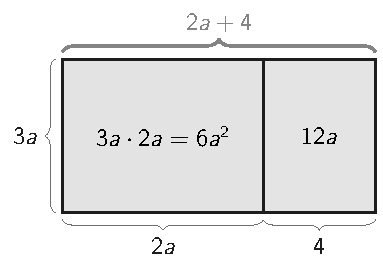
\includegraphics[width=0.95\linewidth]{expr_distributiva}
\end{minipage}
\begin{ojo}[Signos] $(+)(+) = +$, $(-)(-) = +$, $(+)(-) = -$. Así, $-2x(x - 4) = -2x^2 + 8x$. Y al multiplicar se suman exponentes: $x^2\cdot x^3 = x^5$, no $x^6$.\end{ojo}

\subsection{Del lenguaje natural al algebraico}
Lee la frase de afuera hacia adentro: la última operación que se nombra es la que manda. Si la edad de Pedro es $m$, «su edad hace $n$ años disminuida en 3» es $m - n - 3$; «el doble de la suma de un número y 5» es $2(x + 5)$, pero «el doble de un número, más 5» es $2x + 5$.
\begin{center}
\begin{tabular}{@{}ll@{\qquad}ll@{}}
\toprule
En palabras & Expresión & En palabras & Expresión\\ \midrule
el cuadrado de la suma de $a$ y $b$ & $(a + b)^2$ & el triple de la diferencia entre $x$ y 2 & $3(x - 2)$\\
la suma de los cuadrados & $a^2 + b^2$ & dos consecutivos & $n$ y $n + 1$\\
4 menos que $x$ & $x - 4$ & un número par & $2n$\\ \bottomrule
\end{tabular}
\end{center}

\subsection{Perímetros y áreas con expresiones}
Si un rectángulo mide $(2x + 3)$ por $(x - 1)$, su \textbf{perímetro} es $2(2x + 3) + 2(x - 1) = 6x + 4$ y su \textbf{área} es $(2x + 3)(x - 1) = 2x^2 + x - 3$. Con $x = 4$ mide 11 por 3: perímetro 28 y área 33, igual que con las expresiones.
\begin{ojo}[No confundas] El perímetro suma lados (no aparece $x^2$); el área los multiplica. Y para lo que sobra se resta \textbf{todo}, con paréntesis: $(10x + 8) - (6x + 4) = 4x + 4$.\end{ojo}
\gatotip[\gatonaranjo]{¿Dudas entre alternativas? Reemplaza la letra por un número sencillo, como 2, en el enunciado y en cada alternativa: la correcta da lo mismo.}

\begin{elejemplo}{PAES Regular 2026}
Una pista de baile de forma rectangular tiene dimensiones de $(3x + 4)$ metros de largo y $(2x - 9)$ metros de ancho. Se cuenta con $(20x + 20)$ metros de una cinta luminosa para demarcar el borde de la pista de baile.
\begin{center}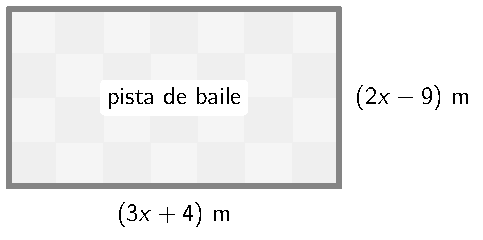
\includegraphics[width=5.2cm]{expr_pista}\end{center}
¿Cuántos metros de cinta luminosa sobran luego de demarcar el borde de la pista?
\alts{$(10x + 30)$ metros}{$(10x + 10)$ metros}{$(15x + 15)$ metros}{$(15x + 25)$ metros}
\solucion{Demarcar el borde es recorrer el perímetro: $2(3x + 4) + 2(2x - 9) = 6x + 8 + 4x - 18 = 10x - 10$. Lo que sobra es la cinta menos todo el perímetro:
\[ (20x + 20) - (10x - 10) = 20x + 20 - 10x + 10 = 10x + 30. \]
Comprobación con $x = 10$: la pista mide 34 m por 11 m, su perímetro es 90 m, la cinta mide 220 m y sobran 130 m $= 10\cdot 10 + 30$. $(10x + 10)$ cambia solo el primer signo del paréntesis; $(15x + 25)$ y $(15x + 15)$ restan medio perímetro.}{A}
\end{elejemplo}

%% =====================================================================
\section{Productos notables}

\subsection{Qué es un producto notable}
Son multiplicaciones tan frecuentes que conviene saber su resultado de memoria. Todas salen de multiplicar término a término, pero reconocer el molde ahorra tiempo y errores de signo.
\begin{clave}[Los cuatro moldes]
\[ (a + b)^2 = a^2 + 2ab + b^2 \qquad (a - b)^2 = a^2 - 2ab + b^2 \]
\[ (a + b)(a - b) = a^2 - b^2 \qquad (x + p)(x + q) = x^2 + (p + q)x + pq \]
Las letras son moldes: en $(2x + 5)^2$, $a = 2x$ y $b = 5$.\end{clave}

\subsection{Cuadrado de binomio}
\begin{minipage}[c]{0.62\linewidth}
En palabras: \textbf{el cuadrado del primero, más (o menos) el doble del primero por el segundo, más el cuadrado del segundo}. El dibujo lo muestra: el cuadrado de lado $a + b$ se parte en $a^2$, $b^2$ y \textbf{dos} rectángulos $ab$.
\[ (x + 5)^2 = x^2 + 10x + 25 \qquad (2x + 3)^2 = 4x^2 + 12x + 9 \]
\[ (x - 4)^2 = x^2 - 8x + 16 \qquad (3x - 2y)^2 = 9x^2 - 12xy + 4y^2 \]
En la resta, el término del medio es negativo y el último \textbf{siempre es positivo}. Además, $(a - b)^2 = (b - a)^2$.
\end{minipage}\hfill
\begin{minipage}[c]{0.34\linewidth}\centering
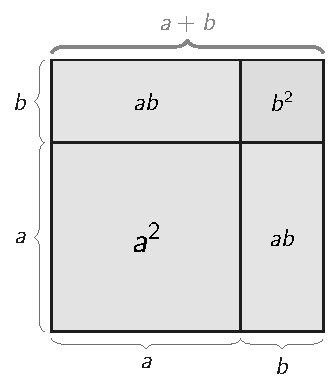
\includegraphics[width=0.85\linewidth]{expr_cuadrado_binomio}
\end{minipage}
\begin{ojo}[El error más común de la PAES] $(a + b)^2 \ne a^2 + b^2$: faltan los dos rectángulos. Con números, $(3 + 4)^2 = 49$, pero $3^2 + 4^2 = 25$. Revisa los tres términos: $(x - 4)^2$ no es $x^2 - 16$, ni $x^2 - 8x - 16$, ni $x^2 - 4x + 16$.\end{ojo}
\gatotip[\gatoatigrado]{Cálculo mental: $21^2 = (20 + 1)^2 = 400 + 40 + 1 = 441$ y $99^2 = (100 - 1)^2 = 10.000 - 200 + 1 = 9801$.}

\subsection{Suma por diferencia}
\begin{minipage}[c]{0.5\linewidth}
Al multiplicar, los términos del medio se cancelan: $(a + b)(a - b) = a^2 - ab + ab - b^2 = a^2 - b^2$. En el dibujo, a un cuadrado de lado $a$ se le quita uno de lado $b$ y lo que queda se reordena en un rectángulo de lados $a + b$ y $a - b$.

$(x + 7)(x - 7) = x^2 - 49$, \quad $(3x + 2y)(3x - 2y) = 9x^2 - 4y^2$ \quad y \quad $103\cdot 97 = 100^2 - 3^2 = 9991$.
\end{minipage}\hfill
\begin{minipage}[c]{0.46\linewidth}\centering
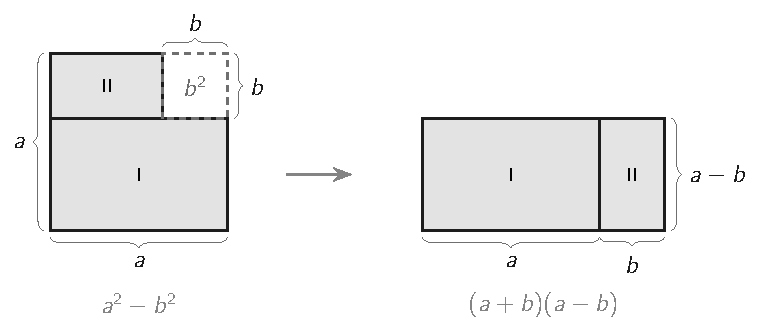
\includegraphics[width=\linewidth]{expr_suma_diferencia}
\end{minipage}
\begin{ojo}[Mismos términos, un signo distinto] $(x + 3)(x - 2)$ no es suma por diferencia.\end{ojo}

\subsection{Binomios con término común}
\begin{minipage}[c]{0.62\linewidth}
En $(x + p)(x + q)$ el resultado es $x^2$, más \textbf{la suma} de los números por $x$, más \textbf{su producto}. En el dibujo, $(x + 4)(x + 3) = x^2 + 7x + 12$.
\[ (x - 5)(x + 2) = x^2 - 3x - 10 \qquad (x - 2)(x - 6) = x^2 - 8x + 12 \]
Si $p = q$ es un cuadrado de binomio; si $q = -p$, una suma por diferencia.
\end{minipage}\hfill
\begin{minipage}[c]{0.34\linewidth}\centering
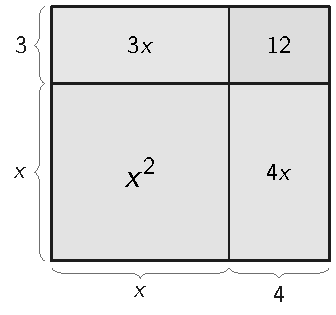
\includegraphics[width=0.8\linewidth]{expr_binomios_comun}
\end{minipage}

\subsection{Combinar productos notables}
Desarrolla cada producto por separado y \textbf{resta con paréntesis}:
\[ (x + 3)^2 - (x + 3)(x - 3) = (x^2 + 6x + 9) - (x^2 - 9) = x^2 + 6x + 9 - x^2 + 9 = 6x + 18. \]
\begin{ejemplo}[Usar datos sin despejar] Si $a + b = 7$ y $ab = 10$: $a^2 + b^2 = (a + b)^2 - 2ab = 49 - 20 = 29$, sin saber cuánto valen $a$ y $b$.\end{ejemplo}
\begin{ojo}[Errores típicos] $(2x)^2 = 4x^2$, no $2x^2$. $(x + 5)^2$ lleva $10x$, no $5x$. $(x + 4)(x - 4) = x^2 - 16$, no $x^2 + 16$. Y al restar $x^2 - 9$, el $-9$ se vuelve $+9$.\end{ojo}
\gatotip[\gatogris]{Comprueba con $x = 1$: la expresión original y tu resultado deben dar el mismo número.}

\begin{elejemplo}{PAES Invierno 2026}
¿Cuál de las siguientes expresiones es igual a $(2x - 3)^2 - (2x - 3)(2x + 3)$?
\alts{$18$}{$0$}{$-6x + 18$}{$-12x + 18$}
\solucion{Cuadrado de binomio con $a = 2x$ y $b = 3$: $(2x - 3)^2 = 4x^2 - 12x + 9$. Suma por diferencia: $(2x - 3)(2x + 3) = 4x^2 - 9$. Restando con paréntesis:
\[ (4x^2 - 12x + 9) - (4x^2 - 9) = 4x^2 - 12x + 9 - 4x^2 + 9 = -12x + 18. \]
Comprobación con $x = 1$: $1 - (-5) = 6$ y $-12 + 18 = 6$. El 18 olvida el término del medio, el 0 cree que los dos productos son iguales y $-6x + 18$ olvida el 2 del doble producto.}{D}
\end{elejemplo}

%% =====================================================================
\section{Factorización}

\subsection{Factorizar es deshacer la multiplicación}
\textbf{Factorizar} es escribir una suma como una multiplicación: el camino inverso de desarrollar. $3a(2a + 4) \to 6a^2 + 12a$ es desarrollar; $6a^2 + 12a \to 6a(a + 2)$ es factorizar. Con números ya lo haces: $12 + 20 = 4(3 + 5)$. Siempre se puede comprobar multiplicando.
\begin{ojo}[Factoriza completo] $3a(2a + 4)$ es igual a $6a^2 + 12a$, pero en el paréntesis queda un 2 común. La factorización completa saca el \textbf{mayor} factor común: $6a(a + 2)$.\end{ojo}

\subsection{Factor común}
\begin{clave}[Cómo encontrarlo] Números: su MCD. Letras: cada letra que está en \textbf{todos} los términos, con su \textbf{menor} exponente. Después divide cada término por el factor común.\end{clave}
\begin{ejemplo} $12x^3 - 18x^2$: MCD 6 y letra $x^2$, así que $12x^3 - 18x^2 = 6x^2(2x - 3)$. Si un término «desaparece» queda 1: $5x + 5 = 5(x + 1)$. El factor común puede ser un paréntesis: $x(a + b) + 3(a + b) = (a + b)(x + 3)$.\end{ejemplo}
\gatotip[\gatonegro]{Cálculo mental: $37\cdot 13 + 37\cdot 87 = 37(13 + 87) = 3700$. El 37 sale una sola vez.}

\subsection{Diferencia de cuadrados}
\begin{clave} \[ a^2 - b^2 = (a + b)(a - b) \] Dos cuadrados separados por un menos. Se usan sus \textbf{raíces}.\end{clave}
\begin{ejemplo} $x^2 - 49 = (x + 7)(x - 7)$; $9x^2 - 16y^2 = (3x + 4y)(3x - 4y)$; $2x^2 - 50 = 2(x^2 - 25) = 2(x + 5)(x - 5)$; $51^2 - 49^2 = 100\cdot 2 = 200$.\end{ejemplo}
\begin{ojo}[La suma de cuadrados no se factoriza así] $x^2 + 9$ no es $(x + 3)(x - 3)$, que da $x^2 - 9$, ni $(x + 3)^2$, que da $x^2 + 6x + 9$.\end{ojo}

\subsection{Trinomio cuadrado perfecto}
\begin{clave} \[ a^2 + 2ab + b^2 = (a + b)^2 \qquad a^2 - 2ab + b^2 = (a - b)^2 \] Los extremos son cuadrados positivos; saca sus raíces; el término del medio debe ser el \textbf{doble} de su producto, y su signo dice si es suma o resta.\end{clave}
\begin{ejemplo} $x^2 + 10x + 25$: raíces $x$ y 5, y $2\cdot x\cdot 5 = 10x$: es $(x + 5)^2$. $4x^2 - 12x + 9 = (2x - 3)^2$. En cambio, $x^2 + 6x + 25$ no es cuadrado perfecto: el medio debería ser $10x$.\end{ejemplo}

\subsection{Trinomio x² + bx + c}
\begin{minipage}[c]{0.64\linewidth}
\[ x^2 + bx + c = (x + p)(x + q) \quad\text{con}\quad p + q = b,\ \ pq = c \]
Busca \textbf{dos números que multiplicados den $c$ y sumados den $b$}. En $x^2 + 7x + 12$ son 3 y 4: $(x + 3)(x + 4)$, el rectángulo del dibujo.
\begin{clave}[Regla de signos] Si $c$ es positivo, los dos números tienen el signo de $b$: $x^2 - 9x + 20 = (x - 4)(x - 5)$. Si $c$ es negativo, tienen signos distintos: $x^2 - 2x - 15 = (x - 5)(x + 3)$.\end{clave}
\end{minipage}\hfill
\begin{minipage}[c]{0.32\linewidth}\centering
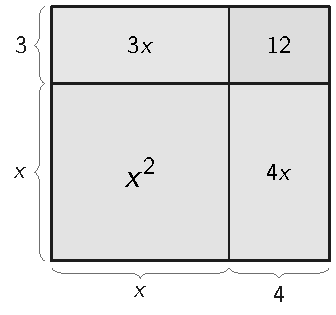
\includegraphics[width=0.85\linewidth]{expr_binomios_comun}
\end{minipage}

\subsection{Simplificar fracciones algebraicas}
Solo se tachan \textbf{factores} (cosas que multiplican), nunca sumandos. Por eso primero se factoriza:
\[ \frac{x^2 - 9}{x + 3} = \frac{(x + 3)(x - 3)}{x + 3} = x - 3 \ \ (x \ne -3), \qquad \frac{x^2 + 5x}{x^2 - 25} = \frac{x(x + 5)}{(x + 5)(x - 5)} = \frac{x}{x - 5}. \]
El valor que anula el denominador original queda excluido también después de simplificar.
\begin{ojo}[Así no] $\dfrac{x + 6}{x + 2} \ne \dfrac{6}{2}$. Con $x = 2$ vale $\dfrac{8}{4} = 2$, no 3.\end{ojo}

\subsection{Qué factorización uso}
\begin{center}
\small\begin{tabular}{@{}lll@{}}
\toprule
Mira esto & Usa & Ejemplo\\ \midrule
algo se repite en todos los términos & factor común (siempre primero) & $4x^2 + 6x = 2x(2x + 3)$\\
dos cuadrados con un menos & diferencia de cuadrados & $x^2 - 36 = (x + 6)(x - 6)$\\
extremos cuadrados y medio $2ab$ & trinomio cuadrado perfecto & $x^2 - 8x + 16 = (x - 4)^2$\\
$x^2 + bx + c$ & producto $c$, suma $b$ & $x^2 + x - 12 = (x + 4)(x - 3)$\\ \bottomrule
\end{tabular}
\end{center}
Después revisa si algún paréntesis se puede factorizar de nuevo: $3x^2 - 12 = 3(x + 2)(x - 2)$ y $2x^3 - 8x^2 + 8x = 2x(x - 2)^2$. Si un producto vale 0, algún factor vale 0: $(p - 3)^2 - 36 = (p + 3)(p - 9) = 0$ da $p = -3$ o $p = 9$.
\gatotip[\gatolila]{Con un área y un lado, factoriza el área: si mide $x^2 + 7x + 12$ y un lado es $x + 3$, el otro es $x + 4$. Y descarta las medidas negativas.}

\begin{elejemplo}{PAES Regular 2026, adaptada}
Una persona realiza el siguiente procedimiento para factorizar $12x^2 + 20x$, cometiendo un error.

Paso 1: escribe cada término como un producto, obteniendo $4\cdot 3\cdot x\cdot x + 4\cdot 5\cdot x$.\\
Paso 2: descompone cada número en factores primos, obteniendo $2\cdot 2\cdot 3\cdot x\cdot x + 2\cdot 2\cdot 5\cdot x$.\\
Paso 3: escribe las potencias correspondientes, obteniendo $2^2\cdot 3\cdot x^2 + 2^2\cdot 5\cdot x$.\\
Paso 4: factoriza la suma, obteniendo $2^4x(3x + 5)$.

¿En cuál de los pasos la persona cometió el error?
\alts{En el Paso 1}{En el Paso 2}{En el Paso 3}{En el Paso 4}
\solucion{Los Pasos 1, 2 y 3 solo reescriben los números: cada expresión sigue siendo igual a $12x^2 + 20x$. En el Paso 4, el factor común es lo que se repite en los dos términos, $2^2$ y $x$, o sea $4x$; la persona sumó los exponentes de los dos $2^2$ y escribió $2^4 = 16$. Lo que se repite se saca \textbf{una vez}. Lo correcto es $12x^2 + 20x = 4x(3x + 5)$; en cambio, $2^4x(3x + 5) = 48x^2 + 80x$, el cuádruple de lo pedido.}{D}
\end{elejemplo}

%% =====================================================================
\section{Proporcionalidad directa}

\subsection{Razón y proporción}
Una \textbf{razón} compara dos cantidades dividiéndolas: 12 niñas y 18 niños están en la razón $12 : 18 = \frac{12}{18} = 2 : 3$, es decir, por cada 2 niñas hay 3 niños. Una \textbf{proporción} es una igualdad de razones, como $\frac{2}{3} = \frac{8}{12}$.
\begin{clave}[Propiedad fundamental] $\dfrac{a}{b} = \dfrac{c}{d}$ es lo mismo que $a\cdot d = b\cdot c$ (producto cruzado). Con ella se despeja el término que falta: $\dfrac{x}{15} = \dfrac{2}{3} \Rightarrow 3x = 30 \Rightarrow x = 10$.\end{clave}
\begin{ojo}[El orden importa] Cuando dice \textbf{respectivamente}, el primer número va con lo primero que se nombra. Y si la razón es $2 : 3$, el grupo tiene $2 + 3 = 5$ partes: las niñas son $\frac{2}{5}$ del curso, no $\frac{2}{3}$.\end{ojo}

\subsection{Qué es la proporcionalidad directa}
Dos cantidades son \textbf{directamente proporcionales} si, cuando una se multiplica por un número, la otra se multiplica por el \textbf{mismo} número: el doble con el doble, la mitad con la mitad. El cociente es constante:
\begin{clave} \[ \frac{y}{x} = k \qquad\Longleftrightarrow\qquad y = k\cdot x \] La constante $k$ es lo que vale $y$ cuando $x = 1$: el precio de \textbf{un} cuaderno, lo que se paga por \textbf{un} minuto. Se llama valor unitario.\end{clave}
\begin{center}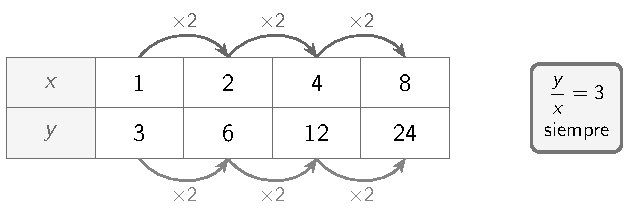
\includegraphics[width=8.2cm]{prop_tabla_directa}\end{center}
\textbf{En una tabla}, divide $y$ por $x$ en cada columna: con $x$: 2, 5, 8 e $y$: 6, 15, 24 siempre da 3, así que es directa. Con $x$: 1, 2, 3 e $y$: 5, 7, 9 da 5; 3,5 y 3: no lo es (es $y = 2x + 3$).
\begin{ojo}[Que las dos crezcan no basta] Al pasar de $x = 1$ a $x = 2$, $y$ debe duplicarse. Además, si $x = 0$, entonces $y = 0$: con un cobro fijo (la bajada de bandera de un taxi) ya no es proporcional.\end{ojo}

\subsection{El gráfico: una recta que pasa por el origen}
\begin{minipage}[c]{0.5\linewidth}
Los puntos $(x, y)$ de $y = kx$ quedan sobre una recta que pasa por $(0, 0)$. Para leer $k$, toma un punto distinto del origen y divide su altura por su $x$: con $(4, 12)$, $k = 3$. Cada vez que avanzas 1, la recta sube $k$: $k$ es la pendiente.

En cambio, $y = 3x + 2$ también es una recta, pero corta el eje $Y$ en 2: no es proporcionalidad directa.
\end{minipage}\hfill
\begin{minipage}[c]{0.46\linewidth}\centering
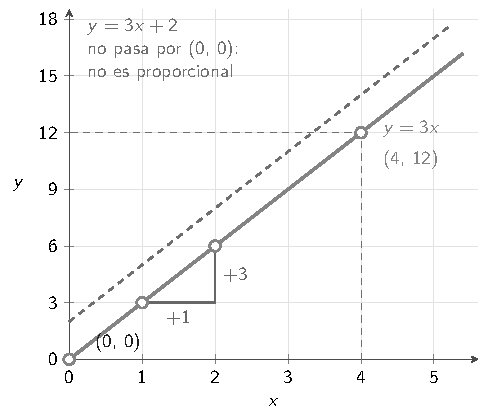
\includegraphics[width=0.92\linewidth]{prop_graf_directa}
\end{minipage}

\subsection{La regla de tres directa}
\begin{ejemplo} 4 kg de paltas cuestan \peso 7200; ¿cuánto cuestan 6 kg? \textbf{Valor unitario:} 1 kg cuesta $\frac{7200}{4} = 1800$, y 6 kg, $6\cdot 1800 = 10.800$. \textbf{Proporción:} $\frac{4}{7200} = \frac{6}{x}$, así que $4x = 43.200$ y $x = 10.800$.\end{ejemplo}
\begin{ojo}[Revisa el sentido] Kilos arriba y pesos abajo en las dos razones. Si te da que 6 kg cuestan menos que 4 kg, armaste mal la proporción. Y si una cantidad aumenta en 100, la otra no aumenta en 100: aumenta en la misma \textbf{proporción}.\end{ojo}
\gatotip[\gatoblanco]{Las escalas de mapas son proporción directa: si 1 cm equivale a 50 m, 7 cm son $7\cdot 50 = 350$ m. Calcula primero lo que vale 1 cm.}

\subsection{Repartos proporcionales}
\begin{clave}[Repartir en la razón $a : b$] Cuenta las partes, $a + b$; divide el total por ese número para obtener una parte, y multiplica por las partes de cada uno.\end{clave}
\begin{ejemplo} \peso 60.000 en la razón $2 : 3$: son 5 partes de 12.000; Ana recibe 24.000 y Beto 36.000. Si se reparte según lo que aportó cada uno (\peso 3000 y \peso 2000), la razón es $3 : 2$.\end{ejemplo}
\begin{ojo}[No dividas por 2] Repartir en la razón $2 : 3$ no es repartir por mitades, ni dividir por 2 y por 3: se divide por el total de partes, 5.\end{ojo}

\begin{elejemplo}{PAES Invierno 2026, adaptada}
Javier y David compraron una bolsa de 24 dulces a un precio total de \peso 2100, tal que Javier aportó \peso 1400 y David aportó el resto del dinero.

Ellos deciden vender cada dulce a \peso 200 y repartirse el dinero obtenido de forma proporcional a lo que aportó cada uno en la compra.

¿Cuánto dinero recibirá Javier luego de vender todos los dulces?
\alts{\peso 1600}{\peso 2400}{\peso 2700}{\peso 3200}
\solucion{La venta da $24\cdot 200 = 4800$ pesos. David aportó $2100 - 1400 = 700$, así que los aportes están en la razón $1400 : 700 = 2 : 1$. Son $2 + 1 = 3$ partes de $\frac{4800}{3} = 1600$, y Javier recibe 2 partes: $3200$ pesos. Comprobación: David recibe 1600 y $3200 + 1600 = 4800$. \peso 1600 es lo de David, \peso 2400 reparte por mitades y \peso 2700 es la ganancia total.}{D}
\end{elejemplo}

%% =====================================================================
\section{Proporcionalidad inversa}

\subsection{Qué es la proporcionalidad inversa}
Dos cantidades son \textbf{inversamente proporcionales} si, cuando una se multiplica por un número, la otra se \textbf{divide} por ese mismo número: si una se duplica, la otra se reduce a la mitad. Al repartir 24 caramelos entre 1, 2, 4 u 8 niños tocan 24, 12, 6 o 3: el producto siempre es 24.
\begin{clave} \[ x\cdot y = k \qquad\Longleftrightarrow\qquad y = \frac{k}{x} \] La constante $k$ es el total: lo que se reparte, la distancia del viaje, el trabajo de la obra.\end{clave}
\begin{center}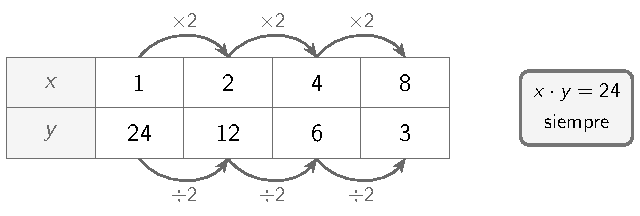
\includegraphics[width=8.2cm]{prop_tabla_inversa}\end{center}

\subsection{Cómo reconocerla}
En una tabla, \textbf{multiplica} $x$ por $y$ en cada columna. A 60 km/h se tarda 4 h, a 80 km/h 3 h y a 120 km/h 2 h: el producto es siempre 240 (la distancia), así que es inversa. Con $x$: 1, 2, 3 e $y$: 10, 8, 6 los productos son 10, 16 y 18: no lo es.
\begin{center}
\begin{tabular}{@{}lll@{}}
\toprule
 & Directa & Inversa\\ \midrule
lo constante & $\dfrac{y}{x} = k$ & $x\cdot y = k$\\[6pt]
fórmula & $y = kx$ & $y = \dfrac{k}{x}$\\[6pt]
si $x$ se duplica & $y$ se duplica & $y$ se divide por 2\\
gráfico & recta por el origen & hipérbola\\ \bottomrule
\end{tabular}
\end{center}
\begin{ojo}[Que una baje cuando la otra sube no basta] En $y = 10 - x$, $y$ baja, pero $1\cdot 9 = 9$ y $2\cdot 8 = 16$. Revisa \textbf{todas} las columnas.\end{ojo}

\subsection{El gráfico: una hipérbola}
\begin{minipage}[c]{0.5\linewidth}
Los puntos de $y = \frac{24}{x}$ forman una curva llamada \textbf{hipérbola}: cuando $x$ crece, $y$ baja, primero rápido y después cada vez más lento. Se acerca a los ejes pero \textbf{nunca los toca}, porque $x$ e $y$ no pueden valer 0.

Desde el origen hasta cada punto se forma un rectángulo de área $x\cdot y = 24$: todos tienen la misma área.
\end{minipage}\hfill
\begin{minipage}[c]{0.46\linewidth}\centering
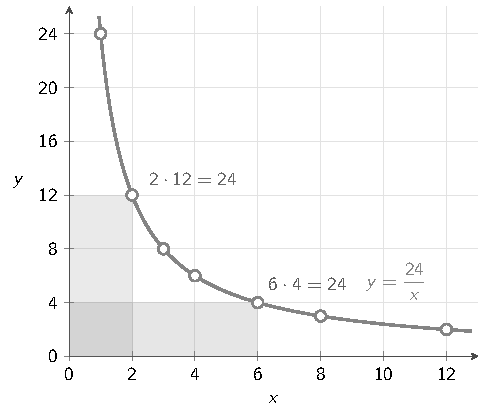
\includegraphics[width=0.92\linewidth]{prop_graf_inversa}
\end{minipage}

\subsection{Trabajadores, rapidez, raciones y llaves}
\begin{clave}[Método] 1. ¿Más de una da menos de la otra? 2. Calcula $k = x\cdot y$, el total. 3. Divide $k$ por la nueva cantidad. 4. Revisa el sentido.\end{clave}
\begin{ejemplo}[Trabajadores] 6 obreros tardan 10 días: la obra son $6\cdot 10 = 60$ «días de un obrero». Con 4 obreros: $\frac{60}{4} = 15$ días. Con proporción, sin dar vuelta nada: $6\cdot 10 = 4\cdot x$.\end{ejemplo}
\begin{ejemplo}[Rapidez, raciones y llaves] A 90 km/h se tarda 4 h: son 360 km, y a 120 km/h se tarda 3 h. Comida para 20 personas por 15 días son 300 raciones: con 25 personas alcanza para 12 días. 3 llaves llenan un estanque en 8 h: son 24 «horas de una llave», y con 4 llaves se tarda 6 h.\end{ejemplo}
\begin{ojo}[El error más común] Hacer regla de tres directa: $\frac{6}{10} = \frac{4}{x}$ da 6,7 días, como si con menos obreros se terminara antes. Todo esto supone el mismo ritmo, que la PAES indica con frases como «en las mismas condiciones».\end{ojo}

\subsection{Dos proporciones a la vez}
Si cambian tres cantidades, ve al \textbf{valor de una unidad}. 4 trabajadores llenan 2000 cajas en 20 días: los 4 llenan $\frac{2000}{20} = 100$ cajas diarias y uno solo, $\frac{100}{4} = 25$. Para 32.000 cajas en 10 días se necesitan 3200 diarias, o sea $\frac{3200}{25} = 128$ trabajadores.
\gatotip[\gatonaranjo]{Lo que hace \emph{uno} se obtiene \emph{dividiendo} lo que hacen todos. Un solo trabajador no puede llenar más cajas que los cuatro juntos.}

\subsection{Directa, inversa o ninguna}
\begin{center}
\begin{tabular}{@{}lll@{}}
\toprule
Situación & Al duplicar $x$ & Tipo\\ \midrule
kilos de pan y precio a pagar & el precio se duplica & directa\\
rapidez y tiempo de un mismo viaje & el tiempo se reduce a la mitad & inversa\\
personas y porción de una torta & la porción se reduce a la mitad & inversa\\
minutos y cobro con cargo fijo & aumenta, pero no al doble & ninguna\\
edad y estatura & no hay regla fija & ninguna\\ \bottomrule
\end{tabular}
\end{center}
\gatotip[\gatogris]{$k$ no es la respuesta: si $x\cdot y = 60$ y $x = 5$, la respuesta es $y = 12$, no 60.}

\begin{elejemplo}{PAES Invierno 2027, adaptada}
En una empresa hay 4 trabajadores para cosechar uvas y estos logran llenar 2000 cajas en 20 días de trabajo, todos trabajando todos los días, al mismo ritmo y la misma cantidad de horas.

En la empresa se realiza el siguiente procedimiento para calcular la cantidad de trabajadores necesarios para llenar 32.000 cajas en 10 días, bajo las mismas condiciones, cometiéndose un error.

Paso 1: se calcula la cantidad de cajas que llenan diariamente los 4 trabajadores en conjunto como $\frac{2000}{20}$, obteniéndose que llenan 100 cajas diarias.\\
Paso 2: se calcula la cantidad de cajas que cada trabajador llena diariamente como $100\cdot 4$, obteniéndose 400 cajas diarias por trabajador.\\
Paso 3: se calcula la cantidad de cajas que se deben llenar diariamente para la nueva producción como $\frac{32.000}{10}$, obteniéndose 3200 cajas diarias.\\
Paso 4: se divide la cantidad de cajas diarias que se deben llenar por la cantidad que cada trabajador llena diariamente como $\frac{3200}{400}$, obteniéndose que se necesitan 8 trabajadores.

¿En cuál de los pasos se cometió el error?
\alts{En el Paso 1}{En el Paso 2}{En el Paso 3}{En el Paso 4}
\solucion{El Paso 1 está bien: $\frac{2000}{20} = 100$ cajas diarias entre los 4. En el Paso 2 está el error: lo que llena \textbf{uno} es $\frac{100}{4} = 25$ cajas diarias; se multiplicó por 4 en vez de dividir. El Paso 3 está bien ($\frac{32.000}{10} = 3200$) y el Paso 4 tiene la idea correcta, pero arrastra el 400. Lo correcto: $\frac{3200}{25} = 128$ trabajadores, que llenan $128\cdot 25 = 3200$ cajas diarias.}{B}
\end{elejemplo}

%% =====================================================================
\section{Sistemas de ecuaciones lineales}

\subsection{Qué es un sistema de ecuaciones}
Un \textbf{sistema} son dos ecuaciones con las mismas dos incógnitas que se deben cumplir \textbf{al mismo tiempo}. Su \textbf{solución} es el par $(x, y)$ que hace verdaderas \textbf{las dos}:
\[ \begin{cases} x + y = 10 \\ x - y = 4 \end{cases} \qquad\text{solución } (7, 3):\quad 7 + 3 = 10,\ \ 7 - 3 = 4. \]
\begin{ojo}[Las dos, no una] $(6, 4)$ cumple la primera, pero no la segunda: no es solución. Y en el par va primero la $x$: $(3, 7)$ es otro par.\end{ojo}

\subsection{Los tres métodos}
\begin{clave}[Sustitución] Despeja una incógnita y \textbf{reemplázala con paréntesis} en la otra ecuación. Conviene cuando una letra tiene coeficiente 1 o $-1$.\end{clave}
\begin{ejemplo} $2x + y = 11$ y $x - 3y = -5$: $y = 11 - 2x$, y $x - 3(11 - 2x) = -5$ da $7x - 33 = -5$, o sea $x = 4$ e $y = 3$.\end{ejemplo}
\begin{clave}[Igualación] Despeja la misma incógnita en las dos e iguala. Conviene cuando las dos vienen como $y = \dots$\end{clave}
\begin{ejemplo} $y = 2x + 1$ e $y = -x + 7$: $2x + 1 = -x + 7$, así que $x = 2$ e $y = 5$.\end{ejemplo}
\begin{clave}[Reducción] Suma las ecuaciones para que una incógnita desaparezca; si hace falta, antes multiplica \textbf{toda} una ecuación. Conviene con coeficientes opuestos.\end{clave}
\begin{ejemplo} $2x + 3y = 12$ y $3x - y = 7$: la segunda por 3 es $9x - 3y = 21$; sumando, $11x = 33$, $x = 3$ e $y = 2$.\end{ejemplo}
\begin{ojo}[Errores típicos] Reemplazar sin paréntesis ($x - 3\cdot 11 - 2x$); multiplicar solo un lado ($9x - 3y = 7$); quedarse con una incógnita o dar vuelta el par. Con fracciones, multiplica antes la ecuación por el mcm.\end{ojo}
\gatotip[\gatoatigrado]{Si te quedas en blanco, reemplaza cada alternativa en las \emph{dos} ecuaciones: la correcta cumple ambas. Y si te dan la solución con letras $a$ y $b$, reemplázala para encontrarlas.}

\subsection{Una, ninguna o infinitas soluciones}
Cada ecuación lineal es una \textbf{recta} y la solución del sistema es el punto donde se cortan (por ejemplo, $x + y = 5$ y $x - y = 1$ se cortan en $(3, 2)$). Dos rectas pueden estar de tres maneras:
\begin{center}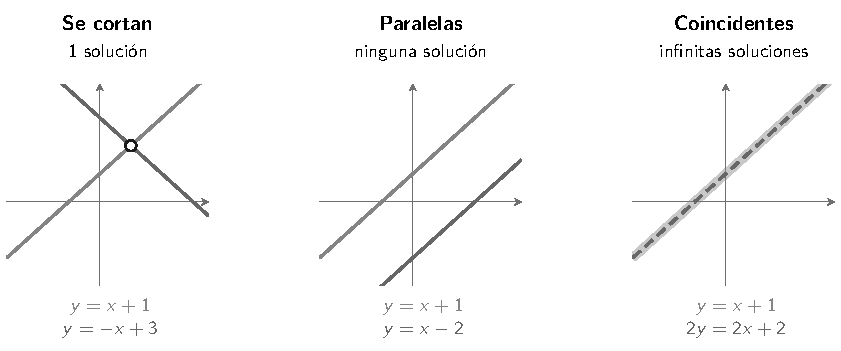
\includegraphics[width=0.85\linewidth]{sis_tres_casos}\end{center}
\begin{center}
\begin{tabular}{@{}llll@{}}
\toprule
Rectas & Despejando $y$ & Soluciones & Al resolver queda\\ \midrule
se cortan & distinta pendiente & una & $x$ e $y$\\
paralelas & misma pendiente, distinto corte & ninguna & algo falso, como $0 = -2$\\
coincidentes & todo igual & infinitas & $0 = 0$\\ \bottomrule
\end{tabular}
\end{center}
\begin{ejemplo} $x + 2y = 3$ y $x + 2y = 5$ son paralelas. $x + 2y = 3$ y $2x + 4y = 6$ son la misma recta: la segunda es la primera multiplicada por 2 en \textbf{todos} sus términos.\end{ejemplo}
\begin{ojo}[Nunca dos] Dos rectas distintas no se cortan en exactamente dos puntos.\end{ojo}

\begin{elejemplo}{Tipo PAES}
¿Cuál es la solución del siguiente sistema de ecuaciones?
\[ \begin{cases} 3x - 2y = 5 \\ x + 4y = 11 \end{cases} \]
\alts{$(2, 3)$}{$(1, -1)$}{$(3, 2)$}{$(7, 1)$}
\solucion{En la segunda la $x$ tiene coeficiente 1: sustitución. $x = 11 - 4y$, y en la primera, $3(11 - 4y) - 2y = 5$, o sea $33 - 14y = 5$, $-14y = -28$ e $y = 2$. Entonces $x = 11 - 8 = 3$. Comprobación: $9 - 4 = 5$ y $3 + 8 = 11$. $(2, 3)$ da vuelta el par, $(1, -1)$ solo cumple la primera y $(7, 1)$ solo la segunda.}{C}
\end{elejemplo}

%% =====================================================================
\section{Problemas con sistemas de ecuaciones}

\subsection{Del enunciado al sistema en 4 pasos}
\begin{clave}[Los 4 pasos] 1. Nombra las dos incógnitas, con su unidad. 2. Escribe una ecuación por cada dato total: casi siempre uno de \textbf{cantidades} y otro de \textbf{valor}. 3. Resuelve. 4. Responde y comprueba en el enunciado.\end{clave}
\begin{ejemplo}[Entradas] Adulto \peso 5000, niño \peso 3000; 80 entradas y \peso 300.000: $x + y = 80$ y $5000x + 3000y = 300.000$. Con $y = 80 - x$ se llega a $2000x = 60.000$: 30 de adulto y 50 de niño.\end{ejemplo}
\begin{ojo}[No mezcles] En la ecuación de cantidades no van precios, y en la de dinero cada cantidad va con \textbf{su} precio. $x + y = 300.000$ no tiene sentido: suma entradas y da pesos.\end{ojo}

\subsection{Monedas, edades y mezclas}
\begin{ejemplo}[Monedas] 30 monedas de \peso 100 y \peso 500 suman \peso 7400: $x + y = 30$ y $100x + 500y = 7400$. Dividiendo la segunda por 100, $x + 5y = 74$; restando la primera, $4y = 44$: 11 de 500 y 19 de 100.\end{ejemplo}
\begin{ejemplo}[Edades] Padre e hijo suman 50; hace 5 años el padre tenía 4 veces la edad del hijo: $p + h = 50$ y $p - 5 = 4(h - 5)$. Resulta $h = 13$ y $p = 37$.\end{ejemplo}
\begin{ojo}[Paréntesis en las edades] «4 veces la edad del hijo hace 5 años» es $4(h - 5)$, no $4h - 5$. Y el tiempo pasa para todos: en 4 años, $a + 4 = 3(h + 4)$.\end{ojo}
\begin{ejemplo}[Mezclas] Café de \peso 8000 y de \peso 12.000 el kilo para 20 kg a \peso 9000: $x + y = 20$ y $8000x + 12.000y = 20\cdot 9000$. Resulta 15 kg del barato y 5 kg del caro: el precio de la mezcla está más cerca del café barato.\end{ejemplo}
\gatotip[\gatolila]{Si el precio es «por kilogramo», la incógnita son \emph{kilogramos}, no frutas ni paquetes. La PAES pregunta justo eso.}

\subsection{Planes: ¿cuándo cuestan lo mismo?}
\begin{minipage}[c]{0.5\linewidth}
Plan A: \peso 8000 más \peso 50 por minuto; plan B: \peso 12.000 más \peso 30. Igualando, $8000 + 50m = 12.000 + 30m$: $m = 200$ minutos, con un costo de \peso 18.000 en ambos.

El punto donde se cortan las rectas es donde las dos cantidades valen lo mismo. Antes de 200 minutos conviene A; después, B.
\end{minipage}\hfill
\begin{minipage}[c]{0.46\linewidth}\centering
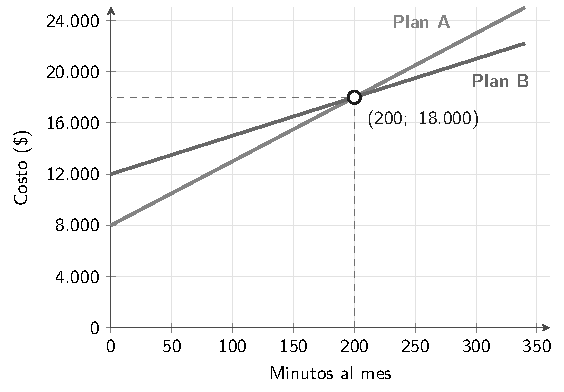
\includegraphics[width=\linewidth]{sis_planes}
\end{minipage}
\begin{ejemplo}[Tarifa fija] Con \peso 2300 por 40 minutos y \peso 3800 por 70: $f + 40v = 2300$ y $f + 70v = 3800$. Restando, $30v = 1500$: $v = 50$ y la tarifa fija es $f = 300$.\end{ejemplo}

\subsection{Qué representa cada parte del sistema}
En una obra de teatro la entrada de niño cuesta \peso 2000 y la de adulto \peso 3500; una familia pagó \peso 40.000 por 14 entradas:
\[ \begin{cases} x + y = 14 \\ 2000x + 3500y = 40.000 \end{cases} \]
\begin{clave}[Cantidad, precio o dinero] $x$ va con 2000: es la \textbf{cantidad} de entradas de niño. 2000 es un \textbf{precio}. $2000x$ es \textbf{dinero}: lo pagado por las entradas de niño. 40.000 es el total pagado y 14 el total de entradas.\end{clave}
\begin{ojo}[Porcentajes] Si aparece $\frac{80}{100}\cdot B$ como lo pagado con un 20~\% de descuento, $B$ es el precio \textbf{original}. Y no sumes lo que el enunciado excluye: «se recaudó solo por las poleras» deja fuera los envíos.\end{ojo}
\gatotip[\gatonegro]{Al final, relee qué representa cada letra: si piden las entradas de niño y respondes $y$, marcaste la otra.}

\begin{elejemplo}{PAES Invierno 2026, adaptada}
Una empresa dedicada a la venta de poleras ofrece a sus clientes dos opciones de diseño: personalizado o de catálogo. El precio por polera con diseño personalizado es \peso 8500 y con diseño de catálogo es \peso 7500. Adicionalmente, se hace un cobro por envío a domicilio de \peso 2500.

En un día de trabajo se vendió un total de 18 poleras en diez envíos y se recaudó \peso 146.000 solo por las poleras. Para calcular la cantidad de poleras con diseño personalizado que se vendieron, una persona realiza el siguiente procedimiento, cometiendo un error.

Paso 1: representa con $x$ la cantidad de poleras con diseño personalizado y con $y$ la cantidad de poleras con diseño de catálogo, y establece el sistema $\begin{cases} x + y = 18 \\ 8500x + 7500y = 146.000 + 25.000 \end{cases}$\\[2pt]
Paso 2: despeja $y$ de la primera ecuación, obteniendo $y = 18 - x$.\\
Paso 3: reemplaza $y$ en la segunda ecuación, obteniendo $8500x - 7500x = 146.000 + 25.000 - 7500\cdot 18$.\\
Paso 4: resuelve la igualdad anterior y determina que la cantidad de poleras con diseño personalizado es 36.

¿En cuál de los pasos la persona cometió el error?
\alts{En el Paso 1}{En el Paso 2}{En el Paso 3}{En el Paso 4}
\solucion{La primera ecuación está bien, pero en la segunda $8500x + 7500y$ es el dinero de las poleras, y el enunciado dice que se recaudaron 146.000 \textbf{solo por las poleras}: los $10\cdot 2500 = 25.000$ de los envíos no van ahí. El error está en el Paso 1. Los Pasos 2, 3 y 4 operan bien con lo que reciben. Lo correcto: $1000x = 146.000 - 135.000 = 11.000$, o sea 11 personalizadas y 7 de catálogo; $8500\cdot 11 + 7500\cdot 7 = 146.000$. Además, 36 poleras personalizadas es imposible si en total se vendieron 18.}{A}
\end{elejemplo}

\chapter{Funciones}
%% Estilo común de los gráficos del capítulo (rectas y parábolas pequeñas).
\pgfplotsset{capfun/.style={width=6.4cm,height=5cm,axis lines=middle,xlabel={$x$},ylabel={$y$},
  every axis x label/.style={at={(ticklabel* cs:1)},anchor=west,font=\small},
  every axis y label/.style={at={(ticklabel* cs:1)},anchor=south,font=\small},
  tick label style={font=\scriptsize},grid=major,grid style={gris!20},samples=120,
  every axis plot/.append style={line width=1.1pt}}}

%% =====================================================================
\section{Concepto de función}
%% =====================================================================

\subsection{Qué es una función}
Una \textbf{función} es una regla que a cada número que entra le asigna \textbf{un solo} número que sale. Al que entra lo llamamos $x$ y al que sale, $f(x)$ («f de x»).
\begin{itemize}
  \item \textbf{Variable independiente}: la $x$, lo que tú eliges.
  \item \textbf{Variable dependiente}: $y = f(x)$, lo que sale; depende de la $x$.
  \item \textbf{Dominio}: los valores que puede tomar la $x$. Si no se dice nada, son todos los números reales.
\end{itemize}
\begin{ejemplo} El kilo de pan cuesta \peso 2.000. Si compro $x$ kilos, pago $f(x) = 2.000\cdot x$. Con 2 kilos: $f(2) = 2.000\cdot 2 = 4.000$ pesos.\end{ejemplo}
\begin{ojo}[Ojo con la escritura] $f(2)$ no es «f por 2»: es lo que sale cuando entra el 2.\end{ojo}

\subsection{Una sola salida para cada entrada}
Un par $(x, y)$ dice «entra $x$, sale $y$». Para que un conjunto de pares sea función, ninguna $x$ puede tener dos salidas distintas.
\begin{clave}[La regla de oro] Dos entradas con la misma salida, como $(1, 5)$ y $(2, 5)$: \textbf{permitido}. Una entrada con dos salidas, como $(1, 5)$ y $(1, 7)$: \textbf{no es función}.\end{clave}
\begin{ejemplo} En $\{(2, 3),\ (5, 3),\ (2, 8)\}$ la entrada $2$ sale una vez $3$ y otra vez $8$: no es función.\end{ejemplo}
En un gráfico se usa una \textbf{recta vertical}: si en algún lugar corta la curva en dos puntos o más, no es función. Una recta horizontal sí puede cortarla varias veces.

\subsection{Evaluar: reemplazar la x}
Evaluar es cambiar \textbf{cada} $x$ de la fórmula por el número, \textbf{entre paréntesis}, y calcular respetando el orden: potencias, multiplicaciones, sumas.
\begin{ejemplo} Si $f(x) = 2x^2 - 7x + 1$:
$f(-3) = 2(-3)^2 - 7(-3) + 1 = 2\cdot 9 + 21 + 1 = 40$.\end{ejemplo}
\begin{ojo}[Tres trampas]
\begin{itemize}
  \item $(-3)^2 = 9$, pero $-3^2 = -(3\cdot 3) = -9$.
  \item $-x^2$ significa $-(x^2)$: si $g(x) = -x^2 + 10$, entonces $g(-3) = -9 + 10 = 1$, no $19$.
  \item $f(2) + f(3)$ no es $f(5)$: con $f(x) = 4x - 1$, $f(2) + f(3) = 7 + 11 = 18$, pero $f(5) = 19$.
\end{itemize}
\end{ojo}
\gatotip[\gatogris]{Reemplaza siempre con paréntesis, aunque el número sea positivo. Con los negativos es lo que te salva: menos por menos da más.}

\subsection{Imagen y preimagen}
Si $f(a) = b$, decimos que $b$ es la \textbf{imagen} de $a$ y que $a$ es una \textbf{preimagen} de $b$.
\begin{clave}[¿Evaluar o despejar?] Si te dan la $x$, \textbf{evalúa}. Si te dan el resultado, \textbf{iguala} la fórmula a ese resultado y despeja la $x$.\end{clave}
\begin{ejemplo} Si $g(x) = 4x + 6$, la preimagen de $26$ sale de $4x + 6 = 26$: $4x = 20$ y $x = 5$. Comprobación: $g(5) = 26$ \checkmark.\end{ejemplo}
Un número puede tener dos preimágenes o ninguna: si $h(x) = x^2$, el $9$ tiene dos ($3$ y $-3$), y el $-4$ no tiene ninguna, porque un cuadrado nunca es negativo. Si en la fórmula falta una constante, un dato como $f(2) = 11$ se convierte en una ecuación para encontrarla.

\subsection{Funciones en tablas y gráficos}
En una tabla, cada fila es un par (entrada, salida). Una fórmula corresponde a la tabla solo si calza en \textbf{todas} las filas. Si la $x$ sube de 1 en 1 y $f(x)$ sube siempre lo mismo, prueba «salto por $x$ más el valor en $x = 0$».

En un gráfico, la entrada se lee en el eje $X$ y la salida es la \textbf{altura}:
\begin{itemize}
  \item $f(a)$: desde $x = a$ sube (o baja) hasta la curva y lee la altura.
  \item $f(x) = b$: traza una horizontal a altura $b$ y, desde cada corte, baja a leer la $x$.
\end{itemize}
\begin{center}
\begin{tikzpicture}
\begin{axis}[capfun,xmin=-3,xmax=3,ymin=-1,ymax=9,xtick={-3,...,3},ytick={0,2,...,8}]
  \addplot[nar,domain=-3:3] {x^2};
  \addplot[azul,dashed,line width=0.8pt,domain=-3:3] {4};
  \draw[menta,dashed,line width=0.8pt] (axis cs:2,0) -- (axis cs:2,4);
  \addplot[only marks,mark=*,mark size=2pt,nard] coordinates {(2,4) (-2,4)};
  \node[font=\scriptsize,anchor=west] at (axis cs:2.05,3.4) {$(2, 4)$};
  \node[font=\scriptsize,anchor=east] at (axis cs:-2.05,3.4) {$(-2, 4)$};
\end{axis}
\end{tikzpicture}
\end{center}
\begin{ejemplo} En el gráfico de $f(x) = x^2$: desde $x = 2$ subo hasta la curva y la altura es $4$, así que $f(2) = 4$. La horizontal a altura $4$ corta la curva en $x = -2$ y $x = 2$: esas son las soluciones de $f(x) = 4$.\end{ejemplo}
\begin{ojo}[Gráficos en contexto] En un gráfico distancia-tiempo, un tramo que sube es avanzar y un tramo \textbf{plano} es estar detenido. Lo que dura la detención se lee restando en el eje del tiempo.\end{ojo}
\gatotip[\gatoatigrado]{Al final, reemplaza tu respuesta en la fórmula. Si sale el dato del enunciado, marcas tranquilo.}

\begin{elejemplo}{PAES Invierno 2026}
Considera la función $g$ definida por $g(x) = 8x - 5$, con dominio el conjunto de los números reales. Si $g(x) = 35$, ¿cuál es el valor de $x$?
\alts{$\dfrac{15}{4}$}{$5$}{$240$}{$275$}
\solucion{Nos dan el resultado, $35$, y buscamos la $x$: igualamos y despejamos. $8x - 5 = 35$; sumamos 5 a los dos lados: $8x = 40$; dividimos por 8: $x = 5$. Comprobación: $g(5) = 40 - 5 = 35$ \checkmark.

¿Por qué no las otras? $\frac{15}{4}$ sale de restar 5 en vez de sumarlo ($8x = 30$). $275$ es $g(35)$: evalúa en vez de despejar. $240$ resta 5 y además multiplica por 8 en vez de dividir.}{B}
\end{elejemplo}

%% =====================================================================
\section{Función lineal y afín}
%% =====================================================================

\subsection{Función afín y función lineal}
Una planta mide 3 cm y crece 2 cm por semana: después de $x$ semanas mide $f(x) = 2x + 3$.
\begin{clave}[Función afín] $f(x) = mx + n$. Su gráfico es una recta. $n = f(0)$ es el \textbf{valor de partida} y $m$ es lo que \textbf{cambia por cada paso} de 1 en $x$.\end{clave}
\begin{clave}[Función lineal] $f(x) = mx$: una afín con $n = 0$. Pasa por el origen y es \textbf{proporcional}: si $x$ se duplica, $y$ se duplica, y $\dfrac{y}{x}$ da siempre $m$.\end{clave}
\begin{ejemplo} Tabla A: $\frac{6}{2} = \frac{12}{4} = \frac{18}{6} = 3$, siempre igual: es lineal, $f(x) = 3x$. Tabla B con los pares $(1, 5)$ y $(2, 7)$: $\frac{5}{1} = 5$ y $\frac{7}{2} = 3{,}5$, distintos: es afín ($2x + 3$).\end{ejemplo}
\begin{ojo}[Afín no es proporcional] En $f(x) = 2x + 3$: $f(1) = 5$ y $f(2) = 7$. La $x$ se duplicó, pero $7$ no es el doble de $5$. Con una afín no sirve la regla de tres. Atajo: si la tabla trae $x = 0$ y su $y$ no es $0$, no es lineal.\end{ojo}
Tampoco son lineales $x^2$ (su gráfico no es recta) ni una constante como $k(x) = 7$ (recta plana a altura 7). Una pendiente negativa o fraccionaria no importa: $g(x) = -\frac{2}{5}x$ sí es lineal.

\subsection{La pendiente}
La \textbf{pendiente} $m$ es cuánto sube (o baja) la recta por cada paso de 1 a la derecha. Con dos puntos es «lo que sube dividido por lo que avanza»:
\begin{clave}[Pendiente con dos puntos] $$m = \frac{y_2 - y_1}{x_2 - x_1}$$\end{clave}
\begin{ejemplo} Por $(1, 4)$ y $(3, 10)$: $m = \dfrac{10 - 4}{3 - 1} = \dfrac{6}{2} = 3$. Por $(-1, 5)$ y $(2, -1)$: $m = \dfrac{-1 - 5}{2 - (-1)} = \dfrac{-6}{3} = -2$.\end{ejemplo}
\begin{ojo}[Las y van arriba] Al revés da $\frac{2}{6}$, que está mal. Y usa el mismo orden arriba y abajo: si los mezclas, el signo sale cambiado.\end{ojo}
\begin{center}
\begin{tikzpicture}
\begin{axis}[capfun,xmin=-3,xmax=3,ymin=-4,ymax=6,xtick={-3,...,3},ytick={-4,-2,...,6}]
  \addplot[nar,domain=-3:3] {2*x} node[pos=0.93,anchor=east,font=\scriptsize] {$m = 2$};
  \addplot[azul,domain=-3:3] {-x+1} node[pos=0.05,anchor=south west,font=\scriptsize] {$m = -1$};
  \addplot[menta,domain=-3:3] {3} node[pos=0.85,anchor=south,font=\scriptsize] {$m = 0$};
\end{axis}
\end{tikzpicture}
\end{center}
\begin{itemize}
  \item $m > 0$: la recta sube, la función es \textbf{creciente}.
  \item $m < 0$: la recta baja, la función es \textbf{decreciente}.
  \item $m = 0$: la recta es horizontal, la función es \textbf{constante}.
\end{itemize}
Mientras más grande es $m$ sin su signo, más inclinada es la recta: $y = 3x$ es más empinada que $y = x$.

\subsection{Cortes con los ejes}
\begin{clave}[Cortes] \textbf{Eje $Y$}: se reemplaza $x = 0$ y queda el punto $(0, n)$. \textbf{Eje $X$}: se iguala a $0$ y se despeja: $mx + n = 0$ da $x = -\dfrac{n}{m}$.\end{clave}
\par\noindent\begin{minipage}{0.55\linewidth}
\begin{ejemplo} Con $f(x) = -3x + 6$: $f(0) = 6$, así que corta al eje $Y$ en $(0, 6)$. Para el eje $X$: $-3x + 6 = 0$, $-3x = -6$, $x = 2$; el punto es $(2, 0)$.\end{ejemplo}
El signo de $n$ dice dónde corta al eje $Y$: $n > 0$ arriba del origen, $n < 0$ abajo, $n = 0$ en el origen (lineal).
\begin{ojo}[No los inviertas] Corte con $Y$: $(0, n)$. Corte con $X$: $(x, 0)$.\end{ojo}
\end{minipage}\hfill
\begin{minipage}{0.4\linewidth}\centering
\begin{tikzpicture}
\begin{axis}[capfun,width=5.6cm,xmin=-1,xmax=4,ymin=-2,ymax=8,xtick={-1,...,4},ytick={-2,0,...,8}]
  \addplot[nar,domain=-1:4] {-3*x+6};
  \addplot[only marks,mark=*,mark size=2pt,nard] coordinates {(0,6) (2,0)};
  \node[font=\scriptsize,anchor=west] at (axis cs:0.1,6.4) {$(0, 6)$};
  \node[font=\scriptsize,anchor=south west] at (axis cs:2.05,0.2) {$(2, 0)$};
\end{axis}
\end{tikzpicture}
\end{minipage}

\subsection{De la tabla o el gráfico a la fórmula}
Primero la pendiente, después $n$ con un punto, y al final se comprueba con otro punto.
\begin{ejemplo}[Desde una tabla] Filas $(1, 5)$, $(3, 11)$ y $(5, 17)$. Avanza 2 y sube 6: $m = 3$. Con $(1, 5)$: $5 = 3 + n$, así que $n = 2$ y $f(x) = 3x + 2$. Comprobación: $f(5) = 17$ \checkmark.\end{ejemplo}
\begin{ejemplo}[Desde un gráfico] La recta corta al eje $Y$ en $(0, -1)$, así que $n = -1$. Pasa justo por la esquina $(2, 3)$: avanza 2 y sube 4, $m = 2$. La fórmula es $f(x) = 2x - 1$.\end{ejemplo}
\begin{ojo}[Un punto no basta] Muchas rectas pasan por un mismo punto. Comprueba siempre con otra fila, y en un gráfico usa puntos exactos de la cuadrícula, no valores «a ojo».\end{ojo}

\subsection{Rectas paralelas y cambios de m y n}
Dos rectas \textbf{paralelas} tienen la \textbf{misma pendiente}.
\begin{ejemplo} La paralela a $y = -x + 2$ que pasa por $(2, 5)$ tiene $m = -1$. Reemplazando el punto: $5 = -2 + n$, así que $n = 7$ y la recta es $y = -x + 7$.\end{ejemplo}
Si cambias $m$ y dejas $n$ fijo, la recta \textbf{gira} en torno a $(0, n)$; si cambias $n$ y dejas $m$, la recta se \textbf{traslada} hacia arriba o hacia abajo, paralela a la anterior.
\gatotip[\gatonegro]{Para leer $m$ y $n$ de un dibujo: ¿sube o baja? Eso es el signo de $m$. ¿Corta al eje $Y$ arriba o abajo del origen? Eso es el signo de $n$.}
\gatotip[\gatolila]{Con una tabla, divide cada $y$ por su $x$. Si siempre da lo mismo, es lineal y basta una regla de tres. Si no, es afín: pendiente, valor de partida y comprobación.}

\begin{elejemplo}{PAES Invierno 2026}
La distancia de reacción es la distancia recorrida por un vehículo desde que el conductor se percata de un obstáculo hasta que comienza a pisar el pedal de freno. La distancia de reacción $f$ y la rapidez del vehículo se relacionan mediante una función de la forma $f(x) = ax$, con $a$ constante. En la siguiente tabla se presentan algunos ejemplos.
\begin{center}
\begin{tabular}{cc}\toprule
Rapidez del vehículo & Distancia de reacción\\\midrule
110 km/h & 33 m\\ 70 km/h & 21 m\\\bottomrule
\end{tabular}
\end{center}
¿Cuál es la distancia de reacción de un vehículo que tiene una rapidez de 30 km/h?
\alts{15 m}{10 m}{9 m}{1 m}
\solucion{Es lineal: la distancia es siempre $a$ veces la rapidez. Con la primera fila, $33 = a\cdot 110$, así que $a = \dfrac{33}{110} = \dfrac{3}{10} = 0{,}3$. Revisamos con la segunda: $0{,}3\cdot 70 = 21$ \checkmark. Entonces $f(30) = 0{,}3\cdot 30 = 9$ m.

¿Por qué no las otras? 15 m usa $a = 0{,}5$; 10 m usa $a = \frac{1}{3}$; 1 m daría $a = \frac{1}{30}$. Ninguna mantiene la razón $0{,}3$ de la tabla.}{C}
\end{elejemplo}

%% =====================================================================
\section{Modelar con funciones afines}
%% =====================================================================

\subsection{Cargo fijo y cargo por unidad}
Muchas cuentas tienen dos partes: un \textbf{cargo fijo}, que se paga una sola vez, y un \textbf{cargo por unidad}, que se paga por cada página, minuto, kilómetro o video.
\begin{ejemplo} Una imprenta cobra \peso 27.000 por preparar el trabajo y \peso 115 por página. Con 0, 1 y 2 páginas: $27.000$; $27.000 + 1\cdot 115$; $27.000 + 2\cdot 115$. Con $x$ páginas: $f(x) = 115x + 27.000$.\end{ejemplo}
\begin{clave}[La forma general] $$f(x) = (\text{precio por unidad})\cdot x + \text{cargo fijo}$$ El precio por unidad es la pendiente; el cargo fijo es el valor con 0 unidades, donde la recta corta al eje $Y$.\end{clave}
\begin{ojo}[Cuidado con la unidad del cobro] Si cobran \peso 400 «por cada media hora», 2 horas son 4 medias horas: $1.500 + 4\cdot 400 = 3.100$. Completa la frase «cobran por cada \underline{\hspace{1cm}}» y cuenta cuántos hay antes de multiplicar.\end{ojo}

\subsection{Usar el modelo: calcular y despejar}
Si te dan la cantidad, reemplaza: $f(100) = 115\cdot 100 + 27.000 = 38.500$. Si te dan el total, iguala, \textbf{resta lo fijo} y divide:
\begin{ejemplo} Pagué \peso 50.000: $115x + 27.000 = 50.000$, $115x = 23.000$, $x = 200$ páginas.\end{ejemplo}
\begin{ojo}[Errores típicos] Escribir $(115 + 27.000)x$ (cobra lo fijo en cada página), escribir $115 + 27.000x$ (cambia lo fijo por lo variable) o dividir $\frac{50.000}{115}$ sin restar antes el cargo fijo.\end{ojo}

\subsection{Cantidades que disminuyen}
Si algo se vacía, se gasta o se consume, a lo inicial se le \textbf{resta} el ritmo por el tiempo:
\begin{ejemplo} Un estanque de 720 L se vacía a 3 L por minuto: $f(x) = -3x + 720$. Quedan 600 L cuando $3x = 120$, o sea a los 40 minutos. Queda vacío cuando $3x = 720$: a los 240 minutos.\end{ejemplo}
La pendiente es negativa porque la cantidad baja; el número solo es lo que había al comienzo.

\subsection{Aumentos iguales y modelos con dos datos}
\begin{ejemplo}[Aumento anual] Un pueblo tenía 4.300 habitantes en 2020 y 4.450 en 2021: aumenta 150 por año. De 2020 a 2028 hay $2028 - 2020 = 8$ aumentos: $4.300 + 8\cdot 150 = 5.500$.\end{ejemplo}
\begin{ejemplo}[Dos datos] Un gasfíter cobra \peso 35.000 por 2 horas y \peso 65.000 por 5 horas. Las 3 horas extra costaron 30.000: cobra $\frac{30.000}{3} = 10.000$ por hora. El fijo es $35.000 - 2\cdot 10.000 = 15.000$. Modelo: $f(x) = 10.000x + 15.000$.\end{ejemplo}
Lo del segundo ejemplo es justo la pendiente: $\dfrac{65.000 - 35.000}{5 - 2}$.
\begin{ojo}[Cuenta bien los años] De 2020 a 2028 hay 8 aumentos, no 9.\end{ojo}

\subsection{Costo, ingreso y ganancia}
\begin{clave}[Tres palabras] \textbf{Costo} $C$: lo que se gasta. \textbf{Ingreso} $I$: lo que entra por ventas. \textbf{Ganancia}: lo que queda, $G = I - C$. Al revés, $C = I - G$.\end{clave}
\begin{ejemplo} Puesto de empanadas: arriendo \peso 20.000, cada empanada cuesta \peso 600 y se vende a \peso 1.500. $C(x) = 600x + 20.000$ e $I(x) = 1.500x$, así que
$G(x) = 1.500x - (600x + 20.000) = 900x - 20.000$. Con 30 empanadas gana $G(30) = 7.000$. Empieza a ganar desde 23 empanadas, porque $900x = 20.000$ da $x \approx 22{,}2$.\end{ejemplo}
\begin{ojo}[El paréntesis] El menos afecta a todo lo que se resta: $-(600x + 20.000) = -600x - 20.000$, y al calcular el costo $-(-20.000) = +20.000$.\end{ojo}

\subsection{Comparar dos planes}
Para saber dónde dos planes cuestan lo mismo, se \textbf{igualan} las dos fórmulas completas.
\par\noindent\begin{minipage}{0.55\linewidth}
\begin{ejemplo} Plan A: \peso 6.000 fijos más \peso 30 por minuto. Plan B: \peso 80 por minuto. $30x + 6.000 = 80x$ da $6.000 = 50x$, o sea $x = 120$. Con menos de 120 minutos conviene B; con más, conviene A.\end{ejemplo}
\begin{ojo}[Si sale con decimales] Si al igualar sale $x \approx 333{,}3$ y piden minutos enteros, el cambio ocurre en el entero siguiente: 334.\end{ojo}
\end{minipage}\hfill
\begin{minipage}{0.4\linewidth}\centering
\begin{tikzpicture}
\begin{axis}[capfun,width=5.8cm,xmin=0,xmax=250,ymin=0,ymax=20,xtick={0,50,...,250},ytick={0,5,...,20},xlabel={min},ylabel={miles de \$}]
  \addplot[nar,domain=0:250] {(6000+30*x)/1000} node[pos=0.9,anchor=north,font=\scriptsize] {A};
  \addplot[azul,domain=0:250] {80*x/1000} node[pos=0.95,anchor=east,font=\scriptsize] {B};
  \addplot[only marks,mark=*,mark size=2pt,nard] coordinates {(120,9.6)};
\end{axis}
\end{tikzpicture}
\end{minipage}

\subsection{Leer gráficos de situaciones}
En un gráfico distancia-tiempo, el eje horizontal es el tiempo y el vertical los kilómetros recorridos desde la partida.
\par\noindent\begin{minipage}{0.55\linewidth}
\begin{itemize}
  \item Tramo que \textbf{sube}: avanza.
  \item Tramo \textbf{plano}: detenido.
  \item Tramo \textbf{más inclinado}: va más rápido.
\end{itemize}
La \textbf{rapidez} de un tramo es lo que avanzó dividido por lo que duró (su pendiente). En el gráfico: de 0 a 1 h, $\frac{60}{1} = 60$ km/h; de 1 a 2,5 h, detenido 1,5 h; de 2,5 a 4 h, $\frac{120}{1{,}5} = 80$ km/h.
\end{minipage}\hfill
\begin{minipage}{0.4\linewidth}\centering
\begin{tikzpicture}
\begin{axis}[capfun,width=5.8cm,xmin=0,xmax=4,ymin=0,ymax=200,xtick={0,1,...,4},ytick={0,40,...,200},xlabel={$t$ (h)},ylabel={km}]
  \addplot[nar,sharp plot] coordinates {(0,0) (1,60) (2.5,60) (4,180)};
  \addplot[only marks,mark=*,mark size=2pt,nard] coordinates {(1,60) (2.5,60) (4,180)};
\end{axis}
\end{tikzpicture}
\end{minipage}
\begin{ojo}[Distancia total] Es la altura del último punto, 180 km. No se suman las alturas, porque cada punto ya muestra todo lo recorrido.\end{ojo}
\gatotip[\gatoblanco]{Antes de marcar, prueba tu fórmula con $x = 0$ y con $x = 1$: con 0 debe dar lo fijo (o lo inicial) y con 1 debe sumar o restar una sola vez el precio por unidad.}

\begin{elejemplo}{PAES Invierno 2027}
Una empresa contrata a una persona para que publique videos mostrando los beneficios de sus productos. La empresa le paga \peso 150.000, más \peso 100.000 por cada video publicado. ¿Cuál de las siguientes funciones modela el dinero que recibirá la persona tras publicar $x$ videos para la empresa?
\alts{$f(x) = 150.000x + 100.000$}{$g(x) = 100.000x + 150.000$}{$h(x) = 100.000\cdot(x + 150.000)$}{$k(x) = x\cdot(100.000 + 150.000)$}
\solucion{Los \peso 150.000 se pagan una sola vez: se suman. Los \peso 100.000 se pagan por cada video: multiplican a $x$. Con 0 videos recibe $150.000$; con 2, $150.000 + 200.000 = 350.000$. El modelo es $g(x) = 100.000x + 150.000$. Comprobación: $g(0) = 150.000$ \checkmark{} y $g(2) = 350.000$ \checkmark.

¿Por qué no las otras? $f$ intercambia lo fijo con lo variable: $f(2) = 400.000$. $h$ multiplica el fijo por 100.000: $h(0)$ es absurdo. $k$ paga el fijo por cada video: $k(0) = 0$.}{B}
\end{elejemplo}

%% =====================================================================
\section{Ecuaciones de segundo grado}
%% =====================================================================

\subsection{La ecuación y sus soluciones}
Una \textbf{ecuación de segundo grado} (o cuadrática) tiene $x^2$ y ninguna potencia mayor. Siempre se puede ordenar como
\begin{clave}[Forma ordenada] $$ax^2 + bx + c = 0,\qquad a \neq 0$$ $a$ acompaña a $x^2$, $b$ acompaña a $x$ y $c$ es el número solo. El signo va pegado al número.\end{clave}
\begin{ejemplo} $x^2 + 6 = 5x$: pasamos el $5x$ restando y ordenamos: $x^2 - 5x + 6 = 0$, con $a = 1$, $b = -5$, $c = 6$.\end{ejemplo}
Una \textbf{solución} es un número que, puesto en lugar de $x$, hace que todo dé $0$. En $x^2 - 5x + 6 = 0$: con $x = 2$, $4 - 10 + 6 = 0$ \checkmark; con $x = 3$, $9 - 15 + 6 = 0$ \checkmark; con $x = 1$ da $2$, así que $1$ no es solución. Normalmente hay dos soluciones; a veces una o ninguna.
\gatotip[\gatonaranjo]{¿En blanco? Reemplaza las alternativas en la ecuación: la correcta es la que hace que todo dé 0.}

\subsection{Los casos fáciles}
Primer paso siempre: \textbf{todo a un lado y un 0 al otro}. Si falta un término, su número es 0.
\begin{clave}[Falta el término con x] Se despeja $x^2$ y se saca raíz, con $+$ y con $-$: $2x^2 = 50$, $x^2 = 25$, $x = \pm 5$.\end{clave}
Casos especiales: $x^2 = 0$ tiene una sola solución, $x = 0$; $x^2 = -9$ no tiene ninguna, porque ningún número al cuadrado da negativo.
\begin{clave}[La regla del cero] Si una multiplicación da 0, al menos un factor es 0: $(x - 4)(x + 1) = 0$ da $x = 4$ o $x = -1$. Solo funciona con un 0 al otro lado.\end{clave}
\begin{clave}[Falta el número solo] Se saca la $x$ factor común: $x^2 = 3x$, $x^2 - 3x = 0$, $x(x - 3) = 0$, así que $x = 0$ o $x = 3$. Una solución es siempre $0$.\end{clave}
\begin{ojo}[Errores clásicos] Quedarse solo con el $5$ positivo. Y dividir $x^2 = 3x$ por $x$: así se pierde la solución $x = 0$.\end{ojo}

\subsection{Factorizar buscando dos números}
Sirve cuando $a = 1$. Como $(x + 2)(x + 3) = x^2 + 5x + 6$, para volver atrás se buscan dos números que \textbf{multiplicados} den $c$ y \textbf{sumados} den $b$.
\begin{ejemplo} $x^2 - 5x + 6 = 0$: $-2$ y $-3$ multiplican $6$ y suman $-5$. Queda $(x - 2)(x - 3) = 0$, así que $x = 2$ o $x = 3$.\end{ejemplo}
\begin{clave}[Los signos en una mirada]
\begin{itemize}
  \item $c$ positivo: los dos números tienen el signo de $b$. En $x^2 + 7x + 10$: $2$ y $5$; en $x^2 - 7x + 10$: $-2$ y $-5$.
  \item $c$ negativo: signos distintos. Busca la pareja que al \textbf{restarse} dé $b$ sin signo; el más grande lleva el signo de $b$. En $x^2 + 3x - 10$: $5$ y $-2$; en $x^2 - 3x - 10$: $-5$ y $2$.
\end{itemize}
\end{clave}
\begin{ojo}[Las soluciones van al revés] $(x + 5)(x - 2) = 0$ da $x = -5$ y $x = 2$: el signo se da vuelta al despejar.\end{ojo}
Con $a = 1$, las dos soluciones multiplicadas dan $c$. Y si conoces una solución, reemplázala en la ecuación para hallar el número que falta.

\subsection{La fórmula general}
Cuando hay un número delante de $x^2$ o no aparecen rápido los dos números, se usa la fórmula, que nunca falla:
\begin{clave}[Fórmula general] $$x = \frac{-b \pm \sqrt{b^2 - 4ac}}{2a}$$\end{clave}
\begin{ejemplo} $2x^2 - 3x - 2 = 0$: $a = 2$, $b = -3$, $c = -2$. Dentro de la raíz: $9 - (-16) = 25$ y $\sqrt{25} = 5$. Luego $x = \dfrac{3 \pm 5}{4}$: sumando da $2$ y restando da $-\frac{1}{2}$.\end{ejemplo}
\begin{ojo}[Tres trampas] $-b$ cambia el signo: si $b = -3$, $-b = 3$. Los negativos van entre paréntesis: $(-3)^2 = 9$. Y $2a$ divide a \textbf{todo} lo de arriba, no solo a la raíz.\end{ojo}

\subsection{El discriminante}
Lo que va dentro de la raíz se llama \textbf{discriminante}, $\Delta = b^2 - 4ac$, y dice cuántas soluciones hay sin resolver.
\par\noindent\begin{minipage}{0.55\linewidth}
\begin{clave}[Cuántas soluciones]
\begin{itemize}
  \item $\Delta > 0$: dos soluciones.
  \item $\Delta = 0$: una sola ($\pm 0$ da lo mismo).
  \item $\Delta < 0$: ninguna solución real.
\end{itemize}
\end{clave}
\begin{ejemplo} $x^2 - 4x + 4$: $\Delta = 16 - 16 = 0$, una solución, $x = \frac{4}{2} = 2$. $x^2 + 2x + 5$: $\Delta = 4 - 20 = -16$, ninguna.\end{ejemplo}
\end{minipage}\hfill
\begin{minipage}{0.4\linewidth}\centering
\begin{tikzpicture}
\begin{axis}[capfun,width=6.2cm,xmin=-1,xmax=7,ymin=-2,ymax=8,xtick={-1,...,5},ytick={-2,0,...,8},
  legend style={font=\scriptsize,at={(0.99,0.03)},anchor=south east,draw=gris!40},legend cell align=left]
  \addplot[nar,domain=-1:5] {x^2-4*x+3}; \addlegendentry{$\Delta>0$}
  \addplot[azul,dashed,domain=-1:5] {x^2-4*x+4}; \addlegendentry{$\Delta=0$}
  \addplot[menta,densely dotted,very thick,domain=-1:5] {x^2-4*x+6}; \addlegendentry{$\Delta<0$}
\end{axis}
\end{tikzpicture}
\end{minipage}

\subsection{Problemas con enunciado}
\begin{enumerate}
  \item Nombra lo que no sabes con una letra.
  \item Escribe lo demás con esa letra: «5 más que $x$» es $x + 5$; «el doble» es $2x$; «el cuadrado» es $x^2$; dos consecutivos son $x$ y $x + 1$.
  \item Plantea la ecuación con el dato, deja un 0 a un lado y resuelve.
  \item Descarta lo que no tiene sentido y responde lo que te piden.
\end{enumerate}
\begin{ejemplo} Terreno con largo 5 m mayor que el ancho y área 104 m$^2$: $x(x + 5) = 104$, $x^2 + 5x - 104 = 0$, $(x + 13)(x - 8) = 0$. El ancho no puede ser $-13$: mide 8 m y el largo 13 m. Perímetro: $8 + 13 + 8 + 13 = 42$ m.\end{ejemplo}
\begin{ojo}[Descarta con criterio] Una medida o un tiempo no pueden ser negativos; si piden «un número», el negativo sí sirve. Y relee la pregunta: si piden el perímetro, 8, 13 o 21 son trampas.\end{ojo}

\begin{elejemplo}{PAES Regular 2026}
Una persona dispone de un terreno de forma rectangular. Se sabe que el terreno tiene un área de 192 m$^2$ y que su ancho mide 4 m menos que su largo. ¿Cuánto mide el largo del terreno?
\alts{12 m}{16 m}{20 m}{24 m}
\solucion{Largo $= L$ y ancho $= L - 4$. El área da $L(L - 4) = 192$, o sea $L^2 - 4L - 192 = 0$. El número solo es negativo: signos distintos, y el más grande lleva el signo de $-4$. Buscamos dos números que multiplicados den 192 y se resten 4: $16$ y $12$. Queda $(L - 16)(L + 12) = 0$, así que $L = 16$ o $L = -12$. Un largo no puede ser negativo: $L = 16$ m. Comprobación: ancho $12$ y $16\cdot 12 = 192$ \checkmark.

¿Por qué no las otras? 12 m es el ancho. Con 20 m el área sería $20\cdot 16 = 320$; con 24 m, $24\cdot 20 = 480$.}{B}
\end{elejemplo}

%% =====================================================================
\section{Gráfico de la función cuadrática}
%% =====================================================================

\subsection{Hacia dónde abre y qué tan abierta es}
Una \textbf{función cuadrática} es $f(x) = ax^2 + bx + c$ con $a \neq 0$. Su gráfico es una curva en forma de U llamada \textbf{parábola}.
\begin{center}
\begin{tikzpicture}
\begin{axis}[capfun,xmin=-3,xmax=3,ymin=-6,ymax=6,xtick={-3,...,3},ytick={-6,-4,...,6}]
  \addplot[nar,domain=-3:3] {x^2} node[pos=0.8,anchor=west,font=\scriptsize] {$x^2$};
  \addplot[azul,domain=-3:3] {-x^2} node[pos=0.8,anchor=west,font=\scriptsize] {$-x^2$};
\end{axis}
\end{tikzpicture}\hspace{6mm}
\begin{tikzpicture}
\begin{axis}[capfun,xmin=-3,xmax=3,ymin=-1,ymax=9,xtick={-3,...,3},ytick={0,2,...,8}]
  \addplot[nar,domain=-3:3] {x^2};
  \addplot[azul,domain=-3:3] {3*x^2};
  \addplot[menta,domain=-3:3] {x^2/2};
  \node[font=\scriptsize,azul,anchor=east] at (axis cs:0.95,6.5) {$3x^2$};
  \node[font=\scriptsize,nard,anchor=west] at (axis cs:2.2,3.5) {$x^2$};
  \node[font=\scriptsize,menta!70!black,anchor=north west] at (axis cs:1.6,1.2) {$\frac{1}{2}x^2$};
\end{axis}
\end{tikzpicture}
\end{center}
\begin{clave}[El número de $x^2$ manda] $a > 0$: abre hacia arriba y el vértice es un \textbf{mínimo}. $a < 0$: abre hacia abajo y el vértice es un \textbf{máximo}. Mientras más grande es $a$ sin su signo, más \textbf{angosta}; si está entre 0 y 1, como $\frac{1}{2}$, es más ancha que $x^2$.\end{clave}
\begin{ojo}[Solo cuenta $a$] En $3 + 5x - 2x^2$ el número de $x^2$ es $-2$: abre hacia abajo. Y el signo no cuenta para el ancho: $-3x^2$ es igual de angosta que $3x^2$.\end{ojo}

\subsection{Corte con el eje Y y tabla de valores}
Al poner $x = 0$, todo lo que tiene $x$ se anula y queda $c$: la parábola corta al eje $Y$ en $(0, c)$. Por ejemplo, $x^2 - 6x + 8$ lo corta en $(0, 8)$, no en $(8, 0)$.

Para dibujarla a mano se hace una tabla. Con $f(x) = x^2 - 2x - 3$:
\begin{center}
\begin{tabular}{c|ccccc}\toprule
$x$ & $-1$ & $0$ & $1$ & $2$ & $3$\\\midrule
$f(x)$ & $1 + 2 - 3 = 0$ & $-3$ & $1 - 2 - 3 = -4$ & $-3$ & $9 - 6 - 3 = 0$\\\bottomrule
\end{tabular}
\end{center}
Las alturas se repiten como en un espejo: $0, -3, -4, -3, 0$. Eso es la simetría de la parábola.

\subsection{Ceros: cortes con el eje X}
Los \textbf{ceros} son las $x$ donde la parábola cruza el eje $X$; ahí la altura es 0, así que se iguala la función a 0.
\begin{ejemplo} $x^2 - 6x + 8 = 0$: $(x - 2)(x - 4) = 0$, así que corta en $(2, 0)$ y $(4, 0)$.\end{ejemplo}
\begin{clave}[¿Cuántas veces corta?] Con $\Delta = b^2 - 4ac$: positivo, dos cortes; cero, la toca en un punto (su vértice); negativo, no la toca.\end{clave}
\begin{ejemplo} Con $a = 1$ y $b = -4$: $x^2 - 4x + 3$ tiene $\Delta = 4$ (dos cortes), $x^2 - 4x + 4$ tiene $\Delta = 0$ (un punto) y $x^2 - 4x + 6$ tiene $\Delta = -8$ (ninguno).\end{ejemplo}

\subsection{El vértice y el eje de simetría}
El \textbf{vértice} es la punta de la parábola. El \textbf{eje de simetría} es la recta vertical que pasa por él y parte la parábola en dos mitades iguales.
\begin{clave}[Vértice] $$x_v = -\frac{b}{2a},\qquad y_v = f(x_v)$$ El eje de simetría es la recta $x = x_v$.\end{clave}
\par\noindent\begin{minipage}{0.55\linewidth}
\begin{ejemplo} $f(x) = x^2 + 2x - 1$: $x_v = -\frac{2}{2} = -1$ e $y_v = 1 - 2 - 1 = -2$. El vértice es $(-1, -2)$; como $a > 0$, el valor mínimo es $-2$ y el eje es $x = -1$.\end{ejemplo}
\begin{clave}[El truco del espejo] Si $f(p) = f(q)$, el eje está en el punto medio: $x = \dfrac{p + q}{2}$. En el dibujo, $f(1) = f(-3) = 2$ y $\frac{1 + (-3)}{2} = -1$.\end{clave}
\end{minipage}\hfill
\begin{minipage}{0.4\linewidth}\centering
\begin{tikzpicture}
\begin{axis}[capfun,width=5.8cm,xmin=-5,xmax=3,ymin=-3,ymax=7,xtick={-5,...,3},ytick={-2,0,...,6}]
  \addplot[nar,domain=-5:3] {x^2+2*x-1};
  \draw[azul,dashed,line width=0.8pt] (axis cs:-1,-3) -- (axis cs:-1,7);
  \addplot[only marks,mark=*,mark size=2pt,nard] coordinates {(-1,-2) (1,2) (-3,2)};
  \node[font=\scriptsize,anchor=west] at (axis cs:-0.8,-2.6) {$(-1, -2)$};
  \node[font=\scriptsize,anchor=west] at (axis cs:1.1,1.7) {$(1, 2)$};
  \node[font=\scriptsize,anchor=east] at (axis cs:-3.1,1.7) {$(-3, 2)$};
\end{axis}
\end{tikzpicture}
\end{minipage}
\begin{ojo}[Ojo con el signo] Si $b$ es negativo, el menos de la fórmula lo vuelve positivo: con $a = 1$ y $b = -6$, $x_v = \frac{6}{2} = 3$. Y se divide por $2a$, no por $a$.\end{ojo}
\gatotip[\gatogris]{El vértice queda justo al medio de los dos ceros. Si ya tienes los ceros, $x_v$ es su promedio: $\frac{-1 + 3}{2} = 1$ en $x^2 - 2x - 3$.}

\subsection{Forma canónica y traslaciones}
\begin{clave}[Forma canónica] $f(x) = a(x - h)^2 + k$ tiene vértice $(h, k)$: el número de \textbf{adentro} con el signo \textbf{cambiado}, el de \textbf{afuera} tal cual.\end{clave}
\begin{ejemplo} $(x - 2)^2 + 1$: el paréntesis vale 0 en $x = 2$ y ahí la función vale 1; vértice $(2, 1)$. En $(x + 3)^2 - 4$ el vértice es $(-3, -4)$.\end{ejemplo}
\par\noindent\begin{minipage}{0.55\linewidth}
Mover la parábola sin cambiar su forma:
\begin{itemize}
  \item Número sumado \textbf{afuera}: $x^2 + 3$ sube 3; $x^2 - 2$ baja 2.
  \item Número \textbf{dentro} del paréntesis: $(x - 2)^2$ se corre 2 a la derecha; $(x + 3)^2$ se corre 3 a la izquierda. Parece al revés, pero lo dicen las cuentas: $(x - 2)^2$ vale 0 en $x = 2$.
\end{itemize}
\end{minipage}\hfill
\begin{minipage}{0.4\linewidth}\centering
\begin{tikzpicture}
\begin{axis}[capfun,width=5.8cm,xmin=-6,xmax=4,ymin=-2.4,ymax=8,xtick={-3,0,2},ytick={2,4,...,8}]
  \addplot[menta,domain=-6:4] {(x+3)^2};
  \addplot[nar,domain=-6:4] {x^2};
  \addplot[azul,domain=-6:4] {(x-2)^2};
  \node[font=\scriptsize,menta!70!black] at (axis cs:-3,-1.7) {$(x+3)^2$};
  \node[font=\scriptsize,azul] at (axis cs:2.4,-1.7) {$(x-2)^2$};
\end{axis}
\end{tikzpicture}
\end{minipage}
\gatotip[\gatoatigrado]{Para reconocer una parábola en un gráfico, descarta en este orden: 1) hacia dónde abre, 2) dónde cruza el eje $Y$, 3) dónde están el vértice o los ceros.}

\begin{elejemplo}{PAES Regular 2026, adaptada}
Considera la función cuadrática $f$, con dominio el conjunto de los números reales. En la figura se representa su gráfica, con su eje de simetría $x = -1$, y el punto $(2, 7)$.
\begin{center}
\begin{tikzpicture}
\begin{axis}[capfun,width=6cm,xmin=-6,xmax=4,ymin=-3,ymax=9,xtick={-6,-4,...,4},ytick={-2,0,...,8}]
  \addplot[nar,domain=-6:4] {x^2+2*x-1} node[pos=0.97,anchor=east,font=\scriptsize] {$f$};
  \draw[azul,dashed,line width=0.8pt] (axis cs:-1,-3) -- (axis cs:-1,9);
  \addplot[only marks,mark=*,mark size=2pt,nard] coordinates {(2,7)};
  \node[font=\scriptsize,anchor=west] at (axis cs:2.1,6.6) {$(2, 7)$};
\end{axis}
\end{tikzpicture}
\end{center}
¿Para cuál de los siguientes valores de $x$ se tiene que $f(x) = 7$?
\alts{$4$}{$-3$}{$-4$}{$-5$}
\solucion{Buscamos el gemelo de $(2, 7)$ al otro lado del eje. Distancia del punto al eje: $2 - (-1) = 3$. El gemelo está 3 unidades a la izquierda: $-1 - 3 = -4$. Entonces $f(-4) = 7$. Comprobación: $\frac{-4 + 2}{2} = -1$ \checkmark.

¿Por qué no las otras? $4$ refleja respecto del eje $Y$ y no de $x = -1$. $-3$ cuenta solo 2 unidades desde el eje; $-5$ cuenta 4.}{C}
\end{elejemplo}

%% =====================================================================
\section{Problemas con función cuadrática}
%% =====================================================================

\subsection{Primero: ¿me piden una x o una y?}
En estos problemas siempre hay una fórmula. La letra de adentro ($x$ o $t$) es lo que eliges: tiempo, unidades vendidas, medida de un lado. El resultado ($y$) es lo que sale: altura, área, ganancia.
\begin{itemize}
  \item «¿Cuándo...?», «¿cuántas unidades...?», «¿qué medida...?»: buscas una $x$.
  \item «¿Qué altura...?», «¿cuánta área o ganancia...?»: buscas una $y$.
\end{itemize}
\begin{ojo}[La trampa favorita] Muchas alternativas incorrectas son la $x$ cuando piden la $y$, o al revés. Decídelo antes de calcular.\end{ojo}

\subsection{Las cuatro preguntas típicas}
\begin{center}
\begin{tabular}{p{6.2cm}p{3.4cm}p{5.6cm}}\toprule
\textbf{Pregunta} & \textbf{En la parábola} & \textbf{Receta}\\\midrule
Valor inicial: ¿desde dónde parte? & corte con el eje $Y$ & $x = 0$: queda el número solo\\
¿Cuándo? ¿Cuántas unidades? & $x$ del vértice & $x_v = -\dfrac{b}{2a}$\\
¿Cuál es el máximo (o mínimo)? & $y$ del vértice & reemplazar $x_v$ en la fórmula\\
Llega al suelo, ni gana ni pierde & ceros & igualar a 0 y despejar\\\bottomrule
\end{tabular}
\end{center}
El orden importa: el máximo necesita primero el «cuándo».

\subsection{Lanzamientos}
\par\noindent\begin{minipage}{0.55\linewidth}
La altura de una pelota es $h(t) = -5t^2 + 20t$ (metros, segundos). Como $a = -5 < 0$, la parábola es un cerro: sube, frena y cae.
\begin{itemize}
  \item Parte de $h(0) = 0$: desde el suelo.
  \item Llega arriba en $t_v = -\dfrac{20}{2\cdot(-5)} = 2$ s.
  \item Altura máxima: $h(2) = -20 + 40 = 20$ m.
  \item Vuelve al suelo: $-5t(t - 4) = 0$, en $t = 4$ s.
\end{itemize}
\end{minipage}\hfill
\begin{minipage}{0.4\linewidth}\centering
\begin{tikzpicture}
\begin{axis}[capfun,width=5.8cm,xmin=0,xmax=4.4,ymin=0,ymax=25,xtick={0,1,...,4},ytick={0,5,...,25},xlabel={$t$},ylabel={$h$}]
  \addplot[nar,domain=0:4] {-5*x^2+20*x};
  \addplot[only marks,mark=*,mark size=2pt,nard] coordinates {(2,20) (0,0) (4,0)};
  \node[font=\scriptsize,anchor=south] at (axis cs:2,20.3) {$(2, 20)$};
\end{axis}
\end{tikzpicture}
\end{minipage}
\begin{ojo}[No confundas] 2 s es \textbf{cuándo} llega arriba; 20 m es \textbf{qué tan alto} llega. Y de los dos ceros, $t = 0$ es el lanzamiento: la respuesta a «¿cuándo vuelve al suelo?» es el otro.\end{ojo}
\begin{ejemplo} En $h(t) = -5t^2 + 10t + 15$, la altura inicial es el número solo: se lanzó desde 15 m. Ojo: eso no es el máximo, porque después sigue subiendo.\end{ejemplo}

\subsection{Áreas máximas}
\begin{ejemplo}[Cerca alrededor] Con 40 m de cerca, un largo más un ancho suman 20. Si un lado es $x$, el otro es $20 - x$ y $A(x) = x(20 - x) = -x^2 + 20x$. Vértice: $x_v = 10$; lados 10 y 10, área 100 m$^2$.\end{ejemplo}
\par\noindent\begin{minipage}{0.6\linewidth}
\begin{ejemplo}[Contra un muro] Con 60 m de malla para tres lados: los dos lados que salen del muro miden $x$ y el de enfrente $60 - 2x$. $A(x) = x(60 - 2x) = -2x^2 + 60x$, $x_v = \frac{60}{4} = 15$, frente $30$ y área $15\cdot 30 = 450$ m$^2$.\end{ejemplo}
\end{minipage}\hfill
\begin{minipage}{0.36\linewidth}\centering
\begin{tikzpicture}[scale=0.75]
  \fill[gris!60] (0,2.4) rectangle (4.4,2.75);
  \node[font=\scriptsize,white] at (2.2,2.58) {muro};
  \draw[nar,line width=1.4pt,fill=hielo] (0.7,2.4) -- (0.7,0.6) -- (3.7,0.6) -- (3.7,2.4);
  \node[font=\small,anchor=east] at (0.65,1.5) {$x$};
  \node[font=\small,anchor=west] at (3.75,1.5) {$x$};
  \node[font=\small,anchor=north] at (2.2,0.55) {$60 - 2x$};
\end{tikzpicture}
\end{minipage}
\begin{ojo}[Con muro no es cuadrado] Si toda la cerca rodea el terreno, el área máxima es siempre un cuadrado. Contra un muro no: el lado de enfrente es el doble de los otros.\end{ojo}
\gatotip[\gatolila]{Si el lado de un cuadrado se multiplica por $k$, el área se multiplica por $k^2$: triplicar el lado multiplica el área por 9.}

\subsection{Ganancias}
\par\noindent\begin{minipage}{0.55\linewidth}
Una empresa gana $G(x) = -x^2 + 40x - 300$ miles de pesos al vender $x$ unidades.
\begin{itemize}
  \item Sin vender: $G(0) = -300$; pierde 300 mil (gastos fijos).
  \item Unidades para la ganancia máxima: $x_v = -\dfrac{40}{-2} = 20$.
  \item Ganancia máxima: $G(20) = -400 + 800 - 300 = 100$ mil pesos.
  \item Ni gana ni pierde: $x^2 - 40x + 300 = 0$ (multiplicando por $-1$), $(x - 10)(x - 30) = 0$: con 10 o 30 unidades.
\end{itemize}
\end{minipage}\hfill
\begin{minipage}{0.4\linewidth}\centering
\begin{tikzpicture}
\begin{axis}[capfun,width=5.8cm,xmin=0,xmax=40,ymin=-300,ymax=150,xtick={0,10,...,40},ytick={-300,-200,...,100},ylabel={$G$}]
  \addplot[nar,domain=0:40] {-x^2+40*x-300};
  \addplot[only marks,mark=*,mark size=2pt,nard] coordinates {(10,0) (30,0) (20,100)};
\end{axis}
\end{tikzpicture}
\end{minipage}
\begin{clave}[¿Dónde se gana?] Si la parábola abre hacia abajo, es positiva \textbf{entre los dos ceros}: aquí, vendiendo entre 10 y 30 unidades.\end{clave}
\begin{ojo}[Ojo con el signo] En $-x^2$ con $x = 20$: primero se eleva y después se pone el menos, $-400$. Y en una fórmula como $d(v) = \frac{v^2}{100}$ también va primero la potencia: $d(80) = \frac{6.400}{100} = 64$.\end{ojo}
\gatotip[\gatonegro]{Revisa que tu respuesta tenga sentido: un tiempo, una medida o una cantidad de personas no pueden ser negativos. Si sale $t^2 = 16$, todavía falta sacar la raíz.}

\begin{elejemplo}{Ejemplo tipo PAES}
La altura $h$, en metros, de una pelota lanzada verticalmente hacia arriba está dada por $h(t) = -5t^2 + 20t$, con $t$ en segundos. ¿Cuál es la altura máxima que alcanza la pelota?
\alts{20 m}{2 m}{40 m}{15 m}
\solucion{Piden una altura, la $y$ del vértice. Con $a = -5$ y $b = 20$: $t_v = -\dfrac{20}{-10} = 2$ s. Reemplazando: $h(2) = -5\cdot 4 + 40 = -20 + 40 = 20$ m. Comprobación: $h(1) = h(3) = 15$, ambas menores que 20 \checkmark.

¿Por qué no las otras? 2 m es el tiempo del vértice (la $x$), no la altura. 40 m olvida la parte $-5t^2$. 15 m es $h(1)$, cuando la pelota todavía sube.}{A}
\end{elejemplo}

\chapter{Geometría}
%% texto a la izquierda y figura a la derecha: \geolado[fracción del ancho para la figura]{figura}{texto}
\newcommand{\geolado}[3][0.38]{\par\smallskip\noindent
  \begin{minipage}[c]{\dimexpr\linewidth-#1\linewidth-14pt\relax}\setlength{\parskip}{4pt}#3\end{minipage}\hspace{14pt}%
  \begin{minipage}[c]{#1\linewidth}\centering\includegraphics[width=\linewidth]{#2}\end{minipage}\par\smallskip}

%% =====================================================================
\section{Teorema de Pitágoras}
\subsection{El triángulo rectángulo y el teorema}
\geolado[0.27]{geo_pit_cuadrados}{Un \textbf{triángulo rectángulo} tiene un ángulo de 90°, que se marca con un cuadradito. Los dos lados que forman ese ángulo son los \textbf{catetos}; el lado que queda al frente es la \textbf{hipotenusa}, y siempre es el más largo.

En la figura, $3^2 + 4^2 = 9 + 16 = 25 = 5^2$: los cuadrados de los catetos juntos tienen la misma área que el cuadrado de la hipotenusa.}
\begin{clave}[Teorema de Pitágoras] Si los catetos miden $a$ y $b$ y la hipotenusa mide $c$, entonces \quad $a^2 + b^2 = c^2$.\end{clave}
\begin{ojo}[Solo para triángulos rectángulos] Si el triángulo no tiene un ángulo de 90°, el teorema no se cumple. Y la hipotenusa va sola en un lado de la igualdad.\end{ojo}

\subsection{Calcular la hipotenusa o un cateto}
\begin{clave}[Regla rápida] Falta la hipotenusa: \textbf{suma} los cuadrados, $c = \sqrt{a^2 + b^2}$. Falta un cateto: \textbf{resta} los cuadrados, al más grande el más chico, $a = \sqrt{c^2 - b^2}$.\end{clave}
\begin{ejemplo} Catetos de 6 cm y 8 cm: $c^2 = 36 + 64 = 100$, así que $c = \sqrt{100} = 10$ cm. Una escalera de 5 m apoyada en un muro, con el pie a 3 m de él, es la hipotenusa: $h^2 = 25 - 9 = 16$ y llega a $h = 4$ m de altura.\end{ejemplo}
\begin{ojo}[La raíz no se reparte] $\sqrt{36 + 64}$ no es $6 + 8 = 14$: primero se suma y después se saca la raíz, $\sqrt{100} = 10$. Además, $c^2 = 100$ todavía no es la respuesta. Si un cateto te sale más largo que la hipotenusa, sumaste cuando había que restar.\end{ojo}
\gatotip[\gatogris]{Antes de hacer cuentas, marca la hipotenusa: es el lado al frente del cuadradito. Escaleras, rampas, tensores y cuerdas inclinadas casi siempre lo son.}

\subsection{Tríos pitagóricos y el recíproco}
Un \textbf{trío pitagórico} son tres enteros que cumplen $a^2 + b^2 = c^2$. Reconocerlos ahorra cuentas, y al multiplicarlos por un mismo número siguen siendo tríos: $6, 8, 10$ es el doble de $3, 4, 5$, y $0{,}7;\ 2{,}4;\ 2{,}5$ es $7, 24, 25$ dividido por 10.
\begin{center}\small
\begin{tabular}{cccccc}\toprule
$3, 4, 5$ & $5, 12, 13$ & $8, 15, 17$ & $7, 24, 25$ & $12, 35, 37$ & $9, 40, 41$\\\bottomrule
\end{tabular}\end{center}
\begin{clave}[Recíproco del teorema] Si el cuadrado del lado mayor es igual a la suma de los cuadrados de los otros dos, el triángulo es rectángulo, y el ángulo recto está al frente del lado mayor.\end{clave}
\begin{ejemplo} Lados 9, 12 y 15: $81 + 144 = 225 = 15^2$ \checkmark, es rectángulo. Lados 4, 5 y 6: $16 + 25 = 41$, pero $6^2 = 36$: no lo es.\end{ejemplo}

\subsection{Diagonales de rectángulos y de cajas}
\geolado[0.42]{geo_pit_diagonales}{La diagonal parte un rectángulo en dos triángulos rectángulos: los lados son los catetos y la diagonal es la hipotenusa. En un cuadrado de lado $\ell$, $d^2 = 2\ell^2$ y $d = \ell\sqrt{2}$.

En una caja de aristas $a$, $b$ y $c$, la diagonal interior cumple \[D^2 = a^2 + b^2 + c^2,\] que sale de aplicar Pitágoras dos veces: primero en el piso y después con la altura.}
\begin{ejemplo} Caja de 2, 3 y 6 cm: $D^2 = 4 + 9 + 36 = 49$, así que $D = 7$ cm. Una pantalla con razón alto\,:\,ancho $= 9 : 16$ tiene alto $9x$ y ancho $16x$, con $x$ el factor de proporcionalidad, y su diagonal cumple $(9x)^2 + (16x)^2 = d^2$.\end{ejemplo}

\subsection{Distancia entre dos puntos del plano}
\geolado[0.33]{geo_pit_distancia}{Para medir la distancia entre $A(4, 2)$ y $B(10, 10)$ se arma un triángulo rectángulo con un cateto horizontal, $10 - 4 = 6$, y uno vertical, $10 - 2 = 8$. Entonces $d = \sqrt{36 + 64} = 10$.}
\begin{clave}[Distancia entre puntos] Entre $(x_1, y_1)$ y $(x_2, y_2)$: \quad $d = \sqrt{(x_2 - x_1)^2 + (y_2 - y_1)^2}$.\end{clave}
\begin{ojo}[Ojo con los negativos] Entre $(-2, 1)$ y $(4, 9)$ el cateto horizontal es $4 - (-2) = 6$, no $2$. Como se eleva al cuadrado, da lo mismo restar en un orden o en el otro.\end{ojo}
\gatotip[\gatoatigrado]{Busca triángulos escondidos: la altura de un triángulo isósceles cae justo al medio de la base, las diagonales de un rombo se cortan por la mitad en ángulo recto y en un trapecio rectángulo el cateto vertical es la diferencia de los lados paralelos.}

\begin{elejemplo}{PAES Invierno 2026, adaptada}
\geolado[0.3]{geo_pit_repisa}{Una persona debe confeccionar una repisa con dos tensores, tal como se representa en la imagen. Cada tensor une el borde superior del panel vertical, de 200 cm de alto, con el borde exterior de la tabla horizontal, de 150 cm de ancho.

Si la persona quiere calcular la medida que debe tener cada uno de los tensores, en centímetros, ¿cuál de las siguientes expresiones debe utilizar?}
\alts{$\sqrt{200^2 - 150^2}$}{$200^2 - 150^2$}{$\sqrt{200^2 + 150^2}$}{$200^2 + 150^2$}
\solucion{El panel vertical (200 cm) y la tabla horizontal (150 cm) forman un ángulo recto, y el tensor une sus extremos: está al frente del ángulo recto, así que es la \textbf{hipotenusa}. Si mide $t$, entonces $t^2 = 200^2 + 150^2$ y, sacando raíz, $t = \sqrt{200^2 + 150^2}$.

\textit{Comprobación}: $\sqrt{40.000 + 22.500} = \sqrt{62.500} = 250$ cm, más largo que 200 y que 150, como debe ser una hipotenusa (es el trío 3, 4, 5 multiplicado por 50) \checkmark.

\textit{¿Por qué no las otras?} $\sqrt{200^2 - 150^2}$ resta, como si faltara un cateto: daría unos 132 cm, menos que el panel. $200^2 - 150^2$ y $200^2 + 150^2$ olvidan la raíz: dan el cuadrado del largo, no el largo.}{C}
\end{elejemplo}
\motivacion{Pitágoras lleva más de dos mil años ayudando a estudiantes, y hoy te ayudó a ti. Tres lados, un teorema, cero miedo.}

%% =====================================================================
\section{Perímetro y área de triángulos, paralelogramos y trapecios}
\subsection{Perímetro y área: no son lo mismo}
El \textbf{perímetro} es el largo del borde: la suma de todos los lados, en unidades de largo (cm, m, km). El \textbf{área} mide la superficie de adentro: cuántos cuadraditos de $1 \times 1$ caben, en unidades cuadradas (cm$^2$, m$^2$).
\begin{ejemplo} Rectángulo de 6 cm por 4 cm: perímetro $2(6 + 4) = 20$ cm y área $6 \cdot 4 = 24$ cm$^2$. Cuadrado de lado 5 cm: perímetro $4 \cdot 5 = 20$ cm y área $5^2 = 25$ cm$^2$.\end{ejemplo}
\begin{ojo}[Cuidado con las unidades] El perímetro va en cm y el área en cm$^2$. Antes de calcular, pasa todo a la misma unidad: no multipliques metros por centímetros.\end{ojo}

\subsection{Área del triángulo: la altura correcta}
\geolado[0.45]{geo_ar_alturas}{Todo triángulo es la mitad de un rectángulo (o de un paralelogramo) con su misma base y su misma altura.

La \textbf{altura} es el segmento \textbf{perpendicular} a la base que llega al vértice opuesto; no es un lado inclinado.}
\begin{clave}[Triángulo] $A = \dfrac{b \cdot h}{2}$ \qquad y, al revés, \qquad $h = \dfrac{2A}{b}$.\end{clave}
En un triángulo rectángulo, los catetos son base y altura. En un obtusángulo, la altura puede caer \textbf{fuera}, sobre la prolongación de la base. Si la base está sobre el eje X, la altura es la coordenada $y$ del vértice opuesto.
\begin{ojo}[No olvides dividir por 2] $b \cdot h$ es el área del rectángulo completo; el triángulo es la mitad. Base 10 cm y altura 7 cm: $A = 35$ cm$^2$.\end{ojo}

\subsection{Paralelogramo y rombo}
\geolado[0.36]{geo_ar_paralelogramo}{Si al \textbf{paralelogramo} le cortas el triángulo de un lado y lo pegas al otro, se forma un rectángulo con la misma base y la misma altura: $A = b \cdot h$.

El \textbf{rombo} es un paralelogramo de cuatro lados iguales cuyas diagonales se cortan en ángulo recto: \[A = \frac{D \cdot d}{2}.\]}
\begin{ejemplo} Paralelogramo de base 8, lado inclinado 5 y altura 4: $A = 8 \cdot 4 = 32$; el lado de 5 no se usa en el área, pero sí en el perímetro, $2(8 + 5) = 26$. Rombo de diagonales 10 y 6: $A = \frac{10 \cdot 6}{2} = 30$.\end{ejemplo}
\begin{ojo}[Altura, no lado] El error más común es multiplicar la base por el lado inclinado: $8 \cdot 5 = 40$ es más que el área real.\end{ojo}

\subsection{Trapecio}
\geolado[0.27]{geo_ar_trapecio}{El trapecio tiene un par de lados paralelos, las bases $B$ y $b$; la altura $h$ es la distancia perpendicular entre ellas. Dos trapecios iguales, uno dado vuelta, forman un paralelogramo de base $B + b$.}
\begin{clave}[Trapecio] $A = \dfrac{(B + b) \cdot h}{2}$\end{clave}
En un \textbf{trapecio rectángulo}, un lado no paralelo es perpendicular a las bases: ese lado es la altura. En un \textbf{trapecio isósceles}, si falta la altura, sale con Pitágoras: cada esquina mide $\frac{B - b}{2}$.
\begin{ejemplo} Bases 12 y 8, altura 5: $A = \frac{(12 + 8) \cdot 5}{2} = 50$.\end{ejemplo}
\begin{ojo}[Primero suma las bases] $(B + b)$ va entre paréntesis: $\frac{(12 + 8) \cdot 5}{2}$, no $12 + \frac{8 \cdot 5}{2}$.\end{ojo}

\subsection{Figuras compuestas: sumar o restar}
\geolado[0.42]{geo_ar_compuesta}{\textbf{Sumar}: la casita es un rectángulo de $6 \cdot 4 = 24$ m$^2$ más un triángulo de $\frac{6 \cdot 3}{2} = 9$ m$^2$; en total, 33 m$^2$.

\textbf{Restar}: el marco es un cuadrado de $7 \cdot 7 = 49$ m$^2$ menos el hueco de $3 \cdot 3 = 9$ m$^2$; quedan 40 m$^2$. Una región sombreada casi siempre es total menos blanco.}
\begin{ojo}[El perímetro va por fuera] Solo se recorre el borde de afuera: las líneas interiores no cuentan. Los lados que no se ven se obtienen restando: si el largo total es 8 y un tramo mide 3, el otro mide 5.\end{ojo}
\begin{center}\small
\begin{tabular}{lll}\toprule
Figura & Perímetro & Área\\\midrule
Rectángulo $a \times b$ & $2(a + b)$ & $a \cdot b$\\
Cuadrado de lado $\ell$ & $4\ell$ & $\ell^2$\\
Triángulo & suma de los 3 lados & $\frac{b \cdot h}{2}$\\
Paralelogramo & $2(b + \text{lado})$ & $b \cdot h$\\
Rombo & $4\ell$ & $\frac{D \cdot d}{2}$\\
Trapecio & suma de los 4 lados & $\frac{(B + b) \cdot h}{2}$\\\bottomrule
\end{tabular}\end{center}
\gatotip[\gatonaranjo]{Si todas las medidas se duplican, el área no se duplica: se multiplica por 4. Con un factor $k$, el área se multiplica por $k^2$. Y mismo perímetro no significa misma área.}

\begin{elejemplo}{PAES Regular 2026, adaptada}
\geolado[0.24]{geo_ar_ej_trapecio}{En la figura adjunta se representa un trapecio rectángulo de área $0{,}76$ m$^2$.

¿Cuál es la medida de su altura?}
\alts{1,444 m}{0,80 m}{0,722 m}{0,40 m}
\solucion{Con la fórmula del trapecio y las bases de 1,3 m y 0,6 m: $0{,}76 = \dfrac{(1{,}3 + 0{,}6) \cdot h}{2} = \dfrac{1{,}9\,h}{2}$. Multiplicando ambos lados por 2, $1{,}52 = 1{,}9\,h$, y dividiendo por 1,9, $h = 0{,}8$ m.

\textit{Comprobación}: $\dfrac{(1{,}3 + 0{,}6) \cdot 0{,}8}{2} = \dfrac{1{,}52}{2} = 0{,}76$ m$^2$ \checkmark.

\textit{¿Por qué no las otras?} 1,444 m multiplica en vez de dividir: $0{,}76 \cdot 1{,}9$. 0,722 m hace lo mismo y además divide por 2. 0,40 m olvida el 2 de la fórmula: $0{,}76 \div 1{,}9$.}{B}
\end{elejemplo}
\motivacion{Áreas y perímetros son puntos seguros si conoces las fórmulas. Ya las tienes: ahora solo queda practicarlas.}

%% =====================================================================
\section{Circunferencia y círculo}
\subsection{Circunferencia, círculo, radio y diámetro}
\geolado[0.45]{geo_ci_partes}{La \textbf{circunferencia} es la línea curva: los puntos que están a la misma distancia del \textbf{centro} $O$. El \textbf{círculo} es la región que encierra.
El \textbf{radio} $r$ va del centro a la circunferencia; el \textbf{diámetro} cruza por el centro y mide $d = 2r$; una \textbf{cuerda} une dos puntos de la circunferencia (la más larga es el diámetro).}
\begin{ojo}[¿Me dieron $r$ o $d$?] Muchos errores de la PAES vienen de usar el diámetro como si fuera el radio. Una moneda de 2,6 cm de diámetro tiene radio 1,3 cm.\end{ojo}

\subsection{Perímetro y área}
En toda circunferencia, el largo del borde dividido por el diámetro da el mismo número, $\pi \approx 3{,}14$. Y si cortas el círculo en muchos sectores y los ordenas alternados, se forma casi un paralelogramo de base $\pi r$ y altura $r$.
\begin{clave}[Fórmulas del círculo] Perímetro: $P = 2\pi r = \pi d$ \qquad Área: $A = \pi r^2$ \qquad Al revés: $r = \dfrac{P}{2\pi}$\end{clave}
\begin{ejemplo} Radio 5 cm: $P = 10\pi \approx 31{,}4$ cm y $A = 25\pi \approx 78{,}5$ cm$^2$. Diámetro 8 cm: $r = 4$ y $A = 16\pi$ cm$^2$. Una rueda de 60 cm de diámetro avanza $60\pi \approx 188{,}4$ cm en cada vuelta.\end{ejemplo}
\begin{ojo}[$r^2$ no es $2r$] Con $r = 5$, $r^2 = 25$ y $2r = 10$. $2\pi r$ es el perímetro (cm); $\pi r^2$ es el área (cm$^2$). El cuadrado afecta solo al radio. Si el radio se duplica, el perímetro se duplica, pero el área se multiplica por 4.\end{ojo}
\gatotip[\gatoblanco]{La PAES suele dejar las respuestas en $\pi$, como $16\pi$ cm$^2$. Reemplaza $\pi \approx 3{,}14$ solo si el enunciado lo pide, y al final.}

\subsection{Semicírculos, cuartos y sectores}
Un \textbf{sector circular} es un trozo de pizza: la región entre dos radios. Si su ángulo es $\alpha$, es la fracción $\frac{\alpha}{360°}$ del círculo:
\[A_{\text{sector}} = \frac{\alpha}{360°}\,\pi r^2 \qquad \text{arco} = \frac{\alpha}{360°}\,2\pi r\]
\begin{center}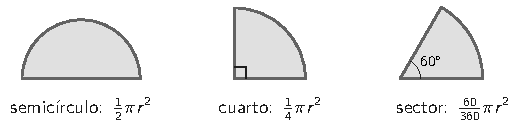
\includegraphics[width=0.5\linewidth]{geo_ci_sectores}\end{center}
\begin{ejemplo} Sector de $60°$ y radio 6: $\frac{60}{360} = \frac{1}{6}$, así que $A = \frac{1}{6} \cdot 36\pi = 6\pi$ y el arco mide $\frac{1}{6} \cdot 12\pi = 2\pi$. Semicírculo: la mitad; cuarto de círculo: la cuarta parte.\end{ejemplo}
\begin{ojo}[No olvides los lados rectos] El borde de un semicírculo es la mitad de la circunferencia \textbf{más el diámetro}: con $r = 5$, $P = 5\pi + 10$. El de un sector incluye los dos radios.\end{ojo}

\subsection{Regiones sombreadas y coronas}
\geolado[0.36]{geo_ci_sombra}{Igual que con los polígonos: área grande menos área en blanco. Un círculo que toca los cuatro lados de un cuadrado de 10 cm tiene radio 5 cm, y lo sombreado mide $100 - 25\pi \approx 21{,}5$ cm$^2$.

La \textbf{corona circular} es el anillo entre dos circunferencias de igual centro y radios $R$ y $r$: \[A = \pi R^2 - \pi r^2 = \pi(R^2 - r^2).\]}
\begin{ojo}[Corona: resta áreas, no radios] Con $R = 5$ y $r = 3$: $\pi(25 - 9) = 16\pi$. En cambio, $\pi(5 - 3)^2 = 4\pi$ está mal.\end{ojo}
\gatotip[\gatonegro]{Cuatro cuartos de círculo iguales forman un círculo completo, y dos semicircunferencias iguales, una circunferencia. ¡Junta los pedazos antes de calcular!}

\begin{elejemplo}{Tipo PAES}
\geolado[0.22]{geo_ci_ej}{En cada esquina de un cuadrado de 8 cm de lado se dibujó un cuarto de círculo con centro en el vértice y radio 4 cm, como se muestra en la figura.

¿Cuál es el área de la región sombreada?}
\alts{$(64 - 4\pi)$ cm$^2$}{$16\pi$ cm$^2$}{$(64 - 16\pi)$ cm$^2$}{$(64 - 8\pi)$ cm$^2$}
\solucion{Lo sombreado es el cuadrado menos los cuatro cuartos de círculo. El cuadrado mide $8 \cdot 8 = 64$ cm$^2$. Los cuatro cuartos, del mismo radio, forman un círculo completo de radio 4: $\pi \cdot 4^2 = 16\pi$ cm$^2$. Queda $(64 - 16\pi)$ cm$^2$.

\textit{Comprobación}: con $\pi \approx 3{,}14$, $16\pi \approx 50{,}24$ y lo sombreado mide unos 13,8 cm$^2$: positivo y menor que lo blanco \checkmark.

\textit{¿Por qué no las otras?} $(64 - 4\pi)$ resta un solo cuarto de círculo. $16\pi$ es la parte en blanco. $(64 - 8\pi)$ usa el perímetro de la circunferencia de radio 4 en vez de su área.}{C}
\end{elejemplo}
\motivacion{Los decimales de $\pi$ no se terminan nunca, y tus ganas tampoco. ¡Una vuelta completa más al temario!}

%% =====================================================================
\section{Área de superficie de cubos, paralelepípedos y cilindros}
\subsection{Los cuerpos y sus partes}
Un \textbf{paralelepípedo} (prisma recto de base rectangular) es una caja: 6 caras rectangulares, iguales de a pares. Un \textbf{cubo} tiene todas sus aristas iguales y sus 6 caras son cuadrados. Ambos tienen \textbf{6 caras, 12 aristas y 8 vértices}. Un \textbf{cilindro} tiene dos bases circulares iguales y una cara lateral curva, como una lata.
\begin{center}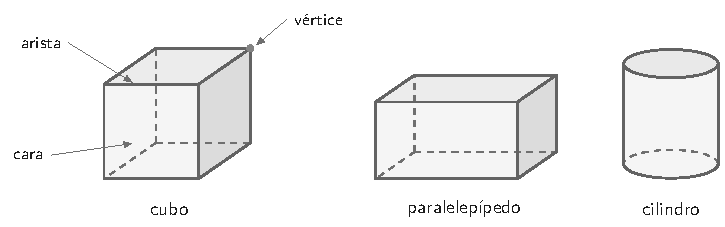
\includegraphics[width=0.62\linewidth]{geo_ac_cuerpos}\end{center}
Las líneas punteadas son aristas ocultas, que quedan detrás.

\subsection{Redes: el cuerpo desarmado}
\geolado[0.38]{geo_ac_redes}{Si desarmas una caja y la estiras sobre la mesa, obtienes su \textbf{red} o desarrollo plano. El \textbf{área de la superficie} del cuerpo es el área de su red: 6 cuadrados iguales en el cubo y 3 pares de rectángulos en el paralelepípedo.

Sirven como red de cubo la cruz y las de forma ``1--4--1''. No sirven un bloque de $2 \times 3$ ni una fila de 4 con dos cuadrados del mismo lado.}
\begin{ojo}[Truco] En una fila de 4 cuadrados, esos 4 son las paredes de alrededor; los otros dos deben ser tapa y fondo, uno a cada lado de la fila.\end{ojo}

\subsection{Área del cubo y del paralelepípedo}
\begin{clave}[Área total] Cubo de arista $a$: $6a^2$. \qquad Paralelepípedo de aristas $a$, $b$, $c$: $2(ab + bc + ac)$.\end{clave}
\begin{ejemplo} Cubo de arista 4 cm: $6 \cdot 16 = 96$ cm$^2$. Al revés, un cubo de 150 cm$^2$ tiene caras de $150 \div 6 = 25$ cm$^2$ y arista $\sqrt{25} = 5$ cm. Caja de 8, 5 y 3 cm: $2(40 + 24 + 15) = 158$ cm$^2$.\end{ejemplo}
Si el cuerpo no tiene tapa, o no se pinta la base, se resta esa cara: el cubo sin tapa tiene $5a^2$.
\begin{ojo}[No confundas con el volumen] El área total del cubo es $6a^2$ (cm$^2$); el volumen es $a^3$ (cm$^3$). Y no olvides el ``por 2'': cada tipo de cara aparece dos veces.\end{ojo}

\subsection{Área del cilindro}
\geolado[0.42]{geo_ac_red_cil}{Al abrir un cilindro, la cara lateral es un \textbf{rectángulo}: su largo es el perímetro de la base, $2\pi r$, y su ancho es la altura $h$. La etiqueta de una lata es justamente el área lateral.}
\begin{clave}[Cilindro] Lateral: $2\pi r h$ \qquad Bases: $2\pi r^2$ \qquad Total: $2\pi r h + 2\pi r^2$\end{clave}
\begin{ejemplo} Lata de radio 3 cm y altura 10 cm: lateral $60\pi$, bases $18\pi$, total $78\pi \approx 244{,}9$ cm$^2$.\end{ejemplo}
\begin{ojo}[Con diámetro] El lateral es $\pi d h$. Si pones el diámetro en lugar del radio en $2\pi r h$, el resultado sale al doble.\end{ojo}
\begin{center}\small
\begin{tabular}{lll}\toprule
Cuerpo & Área lateral & Área total\\\midrule
Cubo de arista $a$ & $4a^2$ & $6a^2$\\
Paralelepípedo $a \times b \times c$ (alto $c$) & $2(a + b)\,c$ & $2(ab + bc + ac)$\\
Cilindro de radio $r$ y altura $h$ & $2\pi r h$ & $2\pi r h + 2\pi r^2$\\\bottomrule
\end{tabular}\end{center}
\gatotip[\gatolila]{Antes de sumar, haz la lista de caras que se cuentan: ``sin tapa'', ``sin la base'', ``solo las paredes''. Y si pegas dos cuerpos, se pierden las \textbf{dos} caras que se tocan.}

\begin{elejemplo}{PAES Invierno 2026, adaptada}
\geolado[0.24]{geo_ac_mueble}{Un carpintero restaurará el siguiente mueble con forma de prisma recto de base rectangular, de 90 cm de ancho, 50 cm de fondo y 200 cm de alto.

Para la restauración, debe pintar el exterior de la estructura, sin incluir la base inferior.

¿Cuál es la medida de la superficie por pintar?}
\alts{32.500 cm$^2$}{56.000 cm$^2$}{60.500 cm$^2$}{65.000 cm$^2$}
\solucion{Calculamos el área total y le restamos la base. Frente y espalda: $2 \cdot (90 \cdot 200) = 36.000$ cm$^2$. Costados: $2 \cdot (50 \cdot 200) = 20.000$ cm$^2$. Tapa y base: $2 \cdot (90 \cdot 50) = 9000$ cm$^2$. Total: $65.000$ cm$^2$. Sin la base inferior: $65.000 - 4500 = 60.500$ cm$^2$.

\textit{Comprobación}, sumando solo lo que se pinta: $36.000 + 20.000 + 4500 = 60.500$ \checkmark.

\textit{¿Por qué no las otras?} 32.500 cm$^2$ cuenta una sola cara de cada par. 56.000 cm$^2$ quita también la tapa, que sí se pinta. 65.000 cm$^2$ incluye la base inferior.}{C}
\end{elejemplo}
\motivacion{Desarmar un cuerpo en sus caras es la clave. Ya ves las figuras por dentro y por fuera.}

%% =====================================================================
\section{Volumen de cubos, paralelepípedos y cilindros}
\subsection{¿Qué es el volumen?}
\geolado[0.28]{geo_vo_cubitos}{El \textbf{volumen} mide cuánto espacio ocupa un cuerpo: cuántos cubitos de $1 \times 1 \times 1$ caben dentro. Se mide en unidades cúbicas: cm$^3$, m$^3$.

En una caja de $4 \times 3 \times 2$ cm caben $4 \cdot 3 = 12$ cubitos en el piso y hay 2 capas: $24$ cm$^3$. Un cubo de arista $a$ tiene $V = a^3$.}
\begin{ojo}[Tres unidades distintas] Largo en cm, área en cm$^2$, volumen en cm$^3$. El volumen siempre es un producto: sumar las aristas no tiene sentido.\end{ojo}

\subsection{Paralelepípedo y cilindro}
\begin{clave}[Volumen = área de la base $\times$ altura] Cubo: $a^3$ \qquad Paralelepípedo: $a \cdot b \cdot c$ \qquad Cilindro: $\pi r^2 h$\end{clave}
\begin{ejemplo} Caja de 20, 5 y 30 cm: $3000$ cm$^3$; si se hace un 10~\% más alta, la altura pasa a 33 cm y el volumen a $3300$ cm$^3$, también un 10~\% más. Lata de radio 3 cm y altura 10 cm: $V = \pi \cdot 9 \cdot 10 = 90\pi \approx 282{,}6$ cm$^3$. Al revés: con $V = 600$, largo 10 y ancho 6, la altura es $600 \div 60 = 10$.\end{ejemplo}
\begin{ojo}[Errores del cilindro] Usar el diámetro como radio (el volumen sale 4 veces más grande), escribir $2\pi r h$ (área lateral) u olvidar elevar el radio al cuadrado. Si el cilindro está acostado, su ``altura'' es el largo.\end{ojo}

\subsection{Capacidad: litros y metros cúbicos}
La \textbf{capacidad} es el volumen que cabe dentro de un recipiente. Un cubo de 10 cm de arista contiene exactamente 1 litro.
\begin{center}\small
\begin{tabular}{ll}\toprule
Volumen & Capacidad\\\midrule
1 cm$^3$ & 1 mL\\
1 dm$^3$ $=$ 1000 cm$^3$ & 1 L\\
1 m$^3$ $=$ 1000 dm$^3$ & 1000 L\\\bottomrule
\end{tabular}\end{center}
\begin{ojo}[Tres medidas, tres veces] De m a cm se multiplica por 100, pero de m$^3$ a cm$^3$ por $100 \cdot 100 \cdot 100 = 1.000.000$. Lo más seguro es pasar las medidas a la unidad que quieras \textbf{antes} de multiplicar.\end{ojo}

\subsection{Llenado, nivel del agua y caudal}
\geolado[0.38]{geo_vo_pecera}{El agua dentro de una caja forma otra caja, con la misma base y de alto el nivel del agua.
\begin{itemize}
\item \textbf{Altura que alcanza}: 6 L $= 6000$ cm$^3$ en una pecera de base $30 \times 20$ cm suben $6000 \div 600 = 10$ cm.
\item \textbf{Objeto sumergido}: si el agua sube 2 cm, su volumen es $30 \cdot 20 \cdot 2 = 1200$ cm$^3$.
\item \textbf{Caudal}: $Q = \frac{V}{t}$. Para llenar 3000 L en 10 minutos se necesitan 300 L/min.
\end{itemize}}
\begin{ojo}[La altura del agua] Si el recipiente no está lleno, usa la altura del agua, no la del recipiente.\end{ojo}

\subsection{Cambios de escala}
\geolado[0.3]{geo_vo_escala}{Si todas las aristas se multiplican por $k$, el volumen se multiplica por $k^3$ (y el área por $k^2$): al duplicar las aristas de un cubo caben $2 \cdot 2 \cdot 2 = 8$ cubos como el original.

Si cambia una sola medida, el volumen cambia en el mismo factor. En $\pi r^2 h$ el radio cuenta doble: duplicarlo multiplica el volumen por 4; duplicar radio y altura, por 8.}
\gatotip[\gatogris]{Si un metal se funde y se rehace en piezas chicas, el volumen se conserva: divide volúmenes. Y para saber cuántas cajas caben en un contenedor, cuenta cuántas entran a lo largo de cada medida y multiplica.}

\begin{elejemplo}{PAES Invierno 2027, adaptada}
\geolado[0.26]{geo_vo_estanque}{Un estanque de agua tiene forma de prisma recto de base rectangular, cuya base mide 4 m de largo y 3 m de ancho. Se debe llenar hasta 2 m de altura con agua proveniente de un ducto.

Para calcular el caudal del agua que sale de un ducto se puede usar la expresión $\frac{V}{t}$, donde $V$ es el volumen de agua que sale del ducto durante $t$ unidades de tiempo.}
¿Cuál de las siguientes expresiones corresponde al caudal de agua, en $\frac{\text{m}^3}{\text{h}}$, que debe salir del ducto para que el estanque se llene hasta 2 m de altura en 10 horas?
\alts{$\dfrac{4 \cdot 3 \cdot 2}{10}$}{$\dfrac{4 + 3 + 2}{10}$}{$\dfrac{2(4 + 3)}{10}$}{$\dfrac{2(4 \cdot 3 + 2 \cdot 4 + 2 \cdot 3)}{10}$}
\solucion{El agua forma una caja de $4 \times 3$ m de base y 2 m de alto: $V = 4 \cdot 3 \cdot 2 = 24$ m$^3$. En $t = 10$ horas, el caudal es $\dfrac{V}{t} = \dfrac{4 \cdot 3 \cdot 2}{10}$, o sea 2,4 m$^3$ por hora.

\textit{Comprobación}: en 10 horas salen $2{,}4 \cdot 10 = 24$ m$^3$ \checkmark.

\textit{¿Por qué no las otras?} $\frac{4 + 3 + 2}{10}$ suma las medidas en vez de multiplicarlas. $\frac{2(4 + 3)}{10}$ usa el perímetro de la base por la altura, que es parte del área lateral. La última usa el área total de la caja: mide superficie, no volumen.}{A}
\end{elejemplo}
\motivacion{Llenaste otro tema hasta el borde. Tu capacidad para aprender es mucho más grande que cualquier cilindro.}

%% =====================================================================
\section{Puntos y vectores en el plano}
\subsection{El plano cartesiano y los cuadrantes}
\geolado[0.34]{tra_plano_cuadrantes}{El \textbf{plano cartesiano} tiene dos rectas numéricas perpendiculares, el \textbf{eje X} (horizontal) y el \textbf{eje Y} (vertical), que se cortan en el \textbf{origen} $O = (0, 0)$. Cada punto es un \textbf{par ordenado} $(x, y)$: primero cuánto avanzas en horizontal, después cuánto subes o bajas. $C(-2, -3)$ está 2 a la izquierda y 3 hacia abajo.

\begin{center}\small
\begin{tabular}{ccc}\toprule
Cuadrante & $x$ & $y$\\\midrule
I (arriba, derecha) & $+$ & $+$\\
II (arriba, izquierda) & $-$ & $+$\\
III (abajo, izquierda) & $-$ & $-$\\
IV (abajo, derecha) & $+$ & $-$\\\bottomrule
\end{tabular}\end{center}}

\subsection{Leer coordenadas sin equivocarse}
\textbf{El orden importa}: $(2, 5)$ y $(5, 2)$ son puntos distintos. Un punto sobre el eje X tiene $y = 0$, como $(4, 0)$; uno sobre el eje Y tiene $x = 0$, como $(0, -3)$. Los puntos de los ejes no son de ningún cuadrante.
\begin{ejemplo} Si $P(a, b)$ está en el cuadrante II, entonces $a < 0$ y $b > 0$. El punto $Q(b, a)$ tiene primera coordenada positiva y segunda negativa: está en el cuadrante IV.\end{ejemplo}
\begin{ojo}[Primero la $x$] En $(x, y)$ siempre va primero lo horizontal, como en el abecedario. Y si la cuadrícula tiene escala, multiplica los cuadros por lo que vale cada uno.\end{ojo}

\subsection{¿Qué es un vector?}
Un \textbf{vector} $\vec{u} = (a, b)$ es una flecha que indica un \textbf{desplazamiento}: $(3, 2)$ es 3 a la derecha y 2 hacia arriba. Tiene \textbf{magnitud} (su largo), \textbf{dirección} (su inclinación) y \textbf{sentido} (hacia cuál lado apunta). Flechas iguales dibujadas en distintos lugares son el mismo vector.
\begin{clave}[Vector opuesto] El opuesto de $(a, b)$ es $(-a, -b)$: misma magnitud y dirección, sentido contrario.\end{clave}

\subsection{El vector entre dos puntos: final menos inicial}
\begin{clave}[Vector de $A$ a $B$] $\overrightarrow{AB} = B - A$ (final menos inicial) \qquad Magnitud de $(a, b)$: $\sqrt{a^2 + b^2}$\end{clave}
\geolado[0.27]{tra_vector_ab}{Con $A(1, 2)$ y $B(5, -1)$: $\overrightarrow{AB} = (5 - 1, -1 - 2) = (4, -3)$: 4 a la derecha y 3 hacia abajo. Su magnitud es $\sqrt{16 + 9} = 5$.


\textit{Comprobación}: $A + (4, -3) = (5, -1) = B$ \checkmark.}
\begin{ojo}[Al revés cambia el signo] $\overrightarrow{BA} = A - B = (-4, 3)$, el opuesto de $\overrightarrow{AB}$. Y la magnitud no es la suma: $|(6, 8)| = \sqrt{100} = 10$, no 14.\end{ojo}

\subsection{Sumar vectores y multiplicarlos por un número}
\geolado[0.27]{tra_suma_vectores}{Se opera coordenada con coordenada: $(a, b) + (c, d) = (a + c, b + d)$ y $k(a, b) = (ka, kb)$.

Con $\vec{u} = (4, 1)$ y $\vec{v} = (1, 3)$: $\vec{u} + \vec{v} = (5, 4)$, $\vec{u} - \vec{v} = (3, -2)$ y $2\vec{u} = (8, 2)$. En el dibujo, la suma es hacer un desplazamiento y después el otro. Multiplicar por un número negativo da vuelta el sentido.}
\begin{ojo}[No se multiplican coordenadas] $(4, 1) + (1, 3)$ no es $(4 \cdot 1, 1 \cdot 3)$.\end{ojo}

\subsection{Trasladar un punto con un vector}
\begin{clave}[Traslación de un punto] $P' = P + \vec{v}$ \qquad y al revés \qquad $P = P' - \vec{v}$\end{clave}
\begin{ejemplo} $P(-3, 4)$ y $\vec{v} = (5, -6)$: $P' = (-3 + 5, 4 - 6) = (2, -2)$. Si $P'(1, 1)$ y $\vec{v} = (4, -2)$, entonces $P = (1 - 4, 1 - (-2)) = (-3, 3)$.\end{ejemplo}
\textbf{Dos traslaciones seguidas} equivalen a una sola con la suma de los vectores: $(2, 1)$ y luego $(3, -4)$ es lo mismo que $(5, -3)$. Con el norte hacia arriba, el este es $x$ positivo, el oeste $x$ negativo, el norte $y$ positivo y el sur $y$ negativo: ``3 km al oeste y 2 km al norte'' es $(-3, 2)$.
\gatotip[\gatonaranjo]{Comprueba siempre: el punto original más el vector debe darte la imagen. Y restar un negativo es sumar: $1 - (-2) = 3$.}
\gatotip[\gatoatigrado]{En un paralelogramo $ABCD$, el vector de $A$ a $D$ es igual al de $B$ a $C$: $D = A + (C - B)$.}

\begin{elejemplo}{PAES Invierno 2026, adaptada}
Un barco que inicia un recorrido realiza los siguientes movimientos, en este orden: 4 kilómetros al oeste, 6 kilómetros al norte, 7 kilómetros al este, 9 kilómetros al sur y 5 kilómetros al oeste.

¿Cuál es la ubicación final del barco con respecto a su ubicación inicial?
\alts{2 kilómetros al este y 3 kilómetros al norte}{16 kilómetros al oeste y 15 kilómetros al sur}{2 kilómetros al oeste y 3 kilómetros al sur}{3 kilómetros al oeste y 2 kilómetros al sur}
\solucion{Cada movimiento es un vector, con este y norte positivos: $(-4, 0)$, $(0, 6)$, $(7, 0)$, $(0, -9)$ y $(-5, 0)$. El desplazamiento total es la suma. Horizontal: $-4 + 7 - 5 = -2$, o sea 2 km al oeste. Vertical: $6 - 9 = -3$, o sea 3 km al sur. El barco termina en $(-2, -3)$: 2 km al oeste y 3 km al sur.
\begin{center}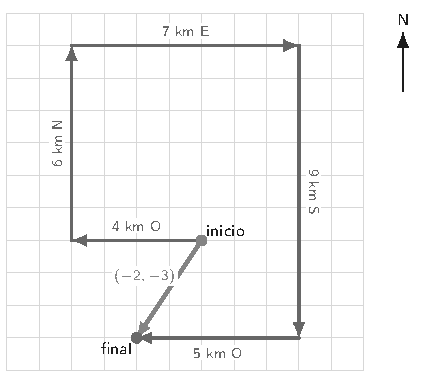
\includegraphics[width=0.3\linewidth]{tra_barco}\end{center}
\textit{Comprobación}: en la cuadrícula, la flecha que une el inicio con el final avanza 2 cuadros a la izquierda y baja 3 \checkmark.

\textit{¿Por qué no las otras?} ``2 al este y 3 al norte'' tiene los sentidos al revés. ``16 al oeste y 15 al sur'' suma todos los kilómetros sin fijarse en el sentido. ``3 al oeste y 2 al sur'' intercambia lo horizontal con lo vertical.}{C}
\end{elejemplo}
\motivacion{Ya te mueves en el plano con coordenadas y vectores. Tu vector apunta directo a la meta.}

%% =====================================================================
\section{Traslación y reflexión}
\subsection{Transformaciones isométricas}
Una \textbf{transformación isométrica} mueve una figura sin deformarla: la imagen tiene la misma forma y el mismo tamaño. Hay tres: \textbf{traslación} (desliza según un vector), \textbf{reflexión} (refleja como un espejo respecto de una recta o de un punto) y \textbf{rotación} (gira en torno a un punto). La imagen del punto $A$ se escribe $A'$.
\begin{center}\small
\begin{tabular}{lccc}\toprule
¿Se conserva? & Traslación & Reflexión & Rotación\\\midrule
Lados, ángulos, perímetro y área & sí & sí & sí\\
Orientación (sentido de recorrido de los vértices) & sí & \textbf{no}, se invierte & sí\\\bottomrule
\end{tabular}\end{center}

\subsection{Traslación de una figura}
\begin{clave}[Traslación según $(a, b)$] $(x, y) \to (x + a, y + b)$\end{clave}
\geolado[0.36]{tra_tras_triangulo}{Se traslada \textbf{cada vértice} con el mismo vector y se unen las imágenes.

Con $A(-5, 1)$, $B(-2, 1)$, $C(-4, 4)$ y $\vec{v} = (6, -3)$: $A'(1, -2)$, $B'(4, -2)$ y $C'(2, 1)$. La figura no gira ni se da vuelta. Si conoces un vértice y su imagen, el vector es imagen menos original.}

\subsection{Reflexión respecto de los ejes}
\geolado[0.3]{tra_refl_ejes}{En una reflexión, cada punto y su imagen quedan a la misma distancia del eje, uno a cada lado, en una línea perpendicular al eje.

\textbf{Respecto del eje X} la $x$ queda igual y la $y$ cambia de signo: $(x, y) \to (x, -y)$; $(3, 5) \to (3, -5)$.

\textbf{Respecto del eje Y} la $y$ queda igual y la $x$ cambia de signo: $(x, y) \to (-x, y)$; $(3, 5) \to (-3, 5)$.

La letra F de la figura queda ``al revés'', como en un espejo.}
\begin{ojo}[Para no confundirte] Cambia la coordenada que \textbf{no} lleva el nombre del eje. Reflejar respecto del eje X manda la figura hacia abajo.\end{ojo}

\subsection{\texorpdfstring{Reflexión respecto de las rectas $x = a$ e $y = b$}{Reflexión respecto de las rectas x = a e y = b}}
\geolado[0.34]{tra_refl_recta}{Cuenta la distancia del punto a la recta y pasa la misma distancia al otro lado. $B(1, 1)$ respecto de $x = 3$: de 1 a 3 hay 2 unidades; $3 + 2 = 5$ y la altura no cambia, $B' = (5, 1)$.}
\begin{clave}[Fórmulas] Respecto de $x = a$: $(x, y) \to (2a - x,\ y)$. \qquad Respecto de $y = b$: $(x, y) \to (x,\ 2b - y)$.\end{clave}
El eje queda justo \textbf{al medio} entre un punto y su imagen: el promedio de 1 y 5 es 3. Así se encuentra el eje si te dan un punto y su imagen.

\subsection{\texorpdfstring{Reflexión respecto de $y = x$ y respecto del origen}{Reflexión respecto de y = x y respecto del origen}}
\geolado[0.32]{tra_refl_yx}{\textbf{Respecto de la recta $y = x$} las coordenadas se intercambian: $(4, 1) \to (1, 4)$ y $(-2, 3) \to (3, -2)$.

\textbf{Respecto del origen} las dos coordenadas cambian de signo: $(4, 1) \to (-4, -1)$. Es lo mismo que reflejar respecto del eje X y luego del eje Y, y que girar $180^\circ$ en torno al origen.}
\begin{center}\small
\begin{tabular}{cccccc}\toprule
eje X & eje Y & recta $x = a$ & recta $y = b$ & recta $y = x$ & origen\\\midrule
$(x, -y)$ & $(-x, y)$ & $(2a - x, y)$ & $(x, 2b - y)$ & $(y, x)$ & $(-x, -y)$\\\bottomrule
\end{tabular}\end{center}
\begin{ojo}[Con $y = x$ no cambian los signos] Solo se intercambian: $(4, -1) \to (-1, 4)$.\end{ojo}

\subsection{Dos transformaciones seguidas}
Se hace la primera y a su resultado se le aplica la segunda. \textbf{El orden importa}.
\begin{ejemplo} $P(2, 3)$: reflexión respecto del eje X, $(2, -3)$, y luego traslación según $(1, 4)$, $(3, 1)$. En el otro orden da $(3, -7)$. Si la regla es $(x + 1, 4 - y)$, eso es reflejar respecto del eje X y trasladar según $(1, 4)$: la imagen de $(5, -2)$ es $(6, 6)$.\end{ejemplo}
\begin{clave}[Dos reflexiones] Respecto del mismo eje dos veces: el punto vuelve. Respecto de dos rectas paralelas: una traslación del doble de la distancia entre ellas. Respecto del eje X y luego del eje Y: la reflexión respecto del origen.\end{clave}
\gatotip[\gatoblanco]{Doblar papel es reflejar: si perforas una hoja doblada, al abrirla la perforación aparece reflejada respecto de la línea del doblez. Para deshacer dos transformaciones, deshazlas en orden inverso.}

\begin{elejemplo}{PAES Invierno 2026, adaptada}
A una figura se le aplica una reflexión y luego una traslación. La imagen del vértice $(x, y)$ es $(x - 3, 4 - y)$. A otra figura se le aplican las mismas transformaciones isométricas y en el mismo orden.

Si $(-2, -5)$ es un vértice de esta figura, ¿cuáles son las coordenadas de la imagen de este vértice?
\alts{$(-5, -1)$}{$(5, 9)$}{$(-5, 9)$}{$(-5, -9)$}
\solucion{Basta reemplazar $x = -2$ e $y = -5$ en la regla: $x - 3 = -2 - 3 = -5$ y $4 - y = 4 - (-5) = 9$. La imagen es $(-5, 9)$.

\textit{Comprobación} por pasos: la regla es una reflexión respecto del eje X seguida de una traslación según $(-3, 4)$; $(-2, -5) \to (-2, 5) \to (-5, 9)$ \checkmark.

\textit{¿Por qué no las otras?} $(-5, -1)$ calcula $4 + y$. $(5, 9)$ cambia el signo de la $x$. $(-5, -9)$ se equivoca con el menos: escribe $4 - (-5)$ como $-(4 + 5)$.}{C}
\end{elejemplo}
\motivacion{Trasladar y reflejar no cambian la figura, solo su lugar. Tú sí estás cambiando: cada tema te hace más fuerte.}

%% =====================================================================
\section{Rotación}
\subsection{¿Qué es una rotación?}
Una \textbf{rotación} gira una figura en torno a un punto fijo, el \textbf{centro de rotación}. Se describe con tres datos: el \textbf{centro} (casi siempre el origen), el \textbf{ángulo} (en la PAES, $90^\circ$, $180^\circ$ o $270^\circ$) y el \textbf{sentido}: \textbf{horario}, como los punteros del reloj, o \textbf{antihorario}, al revés. Cada punto se mantiene a la misma distancia del centro, así que la figura no cambia de tamaño ni se da vuelta.

\subsection{Las reglas de 90°, 180° y 270°}
\geolado[0.34]{tra_rot_tabla}{\begin{center}\small
\begin{tabular}{lcc}\toprule
Rotación en torno al origen & Regla & $P(4, 2)$\\\midrule
$90^\circ$ antihorario & $(-y, x)$ & $(-2, 4)$\\
$180^\circ$ (cualquier sentido) & $(-x, -y)$ & $(-4, -2)$\\
$270^\circ$ antihorario $= 90^\circ$ horario & $(y, -x)$ & $(2, -4)$\\
$360^\circ$ & $(x, y)$ & $(4, 2)$\\\bottomrule
\end{tabular}\end{center}
$270^\circ$ en un sentido es lo mismo que $90^\circ$ en el otro. $180^\circ$ da igual en un sentido o en el otro, y equivale a la reflexión respecto del centro.}
\begin{ejemplo} $90^\circ$ horario a $P(-2, 5)$: $(y, -x) = (5, 2)$. $90^\circ$ antihorario a $(4, -1)$: $(-y, x) = (1, 4)$, porque $-(-1) = 1$.\end{ejemplo}

\subsection{Trucos para no girar al revés}
\begin{clave}[Los cuadrantes] Con $90^\circ$ antihorario, cada punto avanza un cuadrante: I $\to$ II $\to$ III $\to$ IV $\to$ I. Con $90^\circ$ horario retrocede uno. Con $180^\circ$ va al cuadrante opuesto.\end{clave}
También sirve girar la hoja un cuarto de vuelta, o probar con $(1, 0)$: con $90^\circ$ antihorario debe quedar arriba, en $(0, 1)$. Varias rotaciones con el mismo centro se suman: tres de $90^\circ$ antihorario son $270^\circ$, o sea $90^\circ$ horario; cuatro devuelven la figura. Para deshacer una rotación, gira el mismo ángulo en sentido contrario.
\gatotip[\gatolila]{Los punteros del reloj giran en sentido horario, y el minutero avanza $360^\circ \div 60 = 6^\circ$ por minuto: en 20 minutos gira $120^\circ$.}

\subsection{Rotar en torno a otro punto}
\begin{clave}[Centro $C$] Mira el punto desde el centro, gíralo y vuelve: 1. resta el centro, $P - C$; 2. aplica la regla; 3. suma el centro.\end{clave}
\geolado[0.27]{tra_rot_centro}{$P(5, 2)$ en $90^\circ$ antihorario en torno a $C(2, 1)$: $P - C = (3, 1) \to (-1, 3)$, y sumando $C$, $P' = (1, 4)$.}
\begin{ojo}[No olvides volver] Quedarse con $(-1, 3)$ es el error más común: esa es la posición respecto de $C$. Con $180^\circ$, el centro es el punto medio entre el punto y su imagen: $P' = 2C - P$.\end{ojo}

\subsection{¿Qué transformación es?}
\geolado[0.28]{tra_rot_identificar}{Para reconocer qué transformación lleva una figura a otra:

\textbf{1. ¿Está dada vuelta?} Si se ve como en un espejo, es una \textbf{reflexión}.

\textbf{2. Si no, ¿está girada?} Si apunta en otra dirección, es una \textbf{rotación}; si apunta igual y solo cambió de lugar, es una \textbf{traslación}.

Después confirma aplicando la regla a un vértice. La F girada en $180^\circ$ queda cabeza abajo, pero se puede leer girando la hoja; la reflejada no.}
\gatotip[\gatonegro]{Para seguir una flecha, usa ángulos: este $0^\circ$, noreste $45^\circ$, norte $90^\circ$, sur $270^\circ$. Rotar en sentido antihorario suma grados, y una traslación nunca cambia hacia dónde apunta.}

\begin{elejemplo}{PAES Invierno 2027, adaptada}
\geolado[0.32]{tra_rot_proteina}{En el gráfico se representa una simulación bidimensional de una proteína con su grupo metilo, localizado en el punto $P(5, 3)$, con el objetivo de estudiar su desplazamiento. Dicha proteína con su grupo metilo es sometida a una rotación de $90^\circ$ en sentido antihorario con respecto al origen del sistema de coordenadas cartesianas.

¿Cuáles son las coordenadas del grupo metilo después de la rotación?}
\alts{$(3, -5)$}{$(-3, 5)$}{$(-5, -3)$}{$(5, -3)$}
\solucion{La regla de $90^\circ$ antihorario en torno al origen es $(x, y) \to (-y, x)$. Con $x = 5$ e $y = 3$ queda $(-3, 5)$.

\textit{Comprobación}: $P$ estaba en el cuadrante I y la imagen está en el II, como corresponde; además la distancia al origen se mantiene, $\sqrt{25 + 9} = \sqrt{9 + 25} = \sqrt{34}$ \checkmark.

\textit{¿Por qué no las otras?} $(3, -5)$ gira $90^\circ$ en sentido horario. $(-5, -3)$ gira $180^\circ$. $(5, -3)$ refleja respecto del eje X.}{B}
\end{elejemplo}
\motivacion{Girar en 90 o 180 grados ya no es un misterio. Y si algo sale mal, das la vuelta y lo intentas otra vez.}

%% =====================================================================
\section{Semejanza y escalas}
\subsection{Figuras semejantes}
Dos figuras son \textbf{semejantes} ($\sim$) si tienen la misma forma, aunque distinto tamaño: una es ampliación o reducción de la otra. Sus \textbf{ángulos} correspondientes son iguales y sus \textbf{lados} son \textbf{proporcionales}: todos se multiplican por el mismo número $k$, la \textbf{razón de semejanza}.
\begin{center}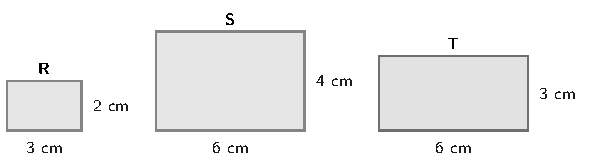
\includegraphics[width=0.52\linewidth]{sem_rectangulos}\end{center}
\begin{ejemplo} $R$ mide $3 \times 2$ y $S$ mide $6 \times 4$: $\frac{6}{3} = \frac{4}{2} = 2$, son semejantes con $k = 2$. $T$ mide $6 \times 3$: $\frac{6}{3} = 2$, pero $\frac{3}{2} = 1{,}5$; no es semejante a $R$.\end{ejemplo}
\begin{ojo}[Proporcional no es sumar lo mismo] Sumarle 3 a cada lado de $3 \times 2$ da $6 \times 5$, que no es semejante. En la semejanza se \textbf{multiplica}.\end{ojo}

\subsection{Lados homólogos y razón de semejanza}
Los \textbf{lados homólogos} son los que se corresponden. Si $\triangle ABC \sim \triangle DEF$, el orden de las letras lo dice: $AB$ con $DE$, $BC$ con $EF$ y $AC$ con $DF$.
\begin{ejemplo} $\triangle ABC \sim \triangle DEF$ con $AB = 3$, $BC = 4$, $AC = 5$, $DE = 6$ y $DF = 10$. La razón es $k = \frac{DE}{AB} = 2$ (y $\frac{DF}{AC} = 2$ lo confirma), así que $EF = 2 \cdot 4 = 8$. Con proporción: $\frac{x}{4} = \frac{6}{3}$, $3x = 24$, $x = 8$.\end{ejemplo}

\subsection{Triángulos semejantes: basta con dos ángulos}
\geolado[0.3]{sem_encajados}{Dos triángulos con \textbf{dos ángulos iguales} son semejantes (criterio AA); el tercero también es igual, porque suman $180^\circ$. También lo son si sus tres lados son proporcionales (LLL) o si dos lados son proporcionales y el ángulo entre ellos es igual (LAL).

Si en $ABC$ se traza $DE$ paralelo a $BC$, el triángulo $ADE$ es semejante a $ABC$. Con $AD = 2$, $DB = 4$ y $DE = 3$: $AB = 6$, $k = \frac{6}{2} = 3$ y $BC = 3 \cdot 3 = 9$.}
\begin{ojo}[El error clásico] El homólogo de $AB$ (lado completo del grande) es $AD$ (lado completo del chico), no el pedazo $DB$.\end{ojo}

\subsection{Sombras, postes y alturas}
\geolado[0.4]{sem_sombras}{A la misma hora, los rayos del sol llegan paralelos: cada objeto vertical, su sombra y el rayo forman triángulos rectángulos semejantes. La razón altura\,:\,sombra es la misma para todos.

Un poste de 4 m da 6 m de sombra. Una persona de 1,6 m da $\frac{1{,}6}{x} = \frac{4}{6}$, o sea $4x = 9{,}6$ y $x = 2{,}4$ m.}
\begin{ojo}[Ordena antes de calcular] Alturas arriba y sombras abajo en las dos fracciones; si mezclas, el resultado sale al revés.\end{ojo}
\gatotip[\gatogris]{Espejos en el suelo, rampas con soportes y ríos que no se pueden cruzar esconden lo mismo: dos triángulos semejantes. Empareja los lados homólogos y escribe la misma razón en ambos.}

\subsection{Planos, mapas y maquetas a escala}
Una \textbf{escala $1 : n$} significa que 1 cm del dibujo representa $n$ cm de la realidad. Del dibujo a la realidad se multiplica por $n$; de la realidad al dibujo se divide.
\begin{ejemplo} Mapa 1\,:\,50.000 con 6 cm entre dos pueblos: $6 \cdot 50.000 = 300.000$ cm $= 3000$ m $= 3$ km. Edificio de 45 m en maqueta 1\,:\,300: $\frac{4500}{300} = 15$ cm. Si 2 cm del mapa son 200 m $= 20.000$ cm, 1 cm son 10.000 cm: escala 1\,:\,10.000.\end{ejemplo}
\begin{ojo}[Mismas unidades] La escala compara centímetros con centímetros: 1 m $= 100$ cm, 1 km $= 100.000$ cm y 1 m$^2$ $= 10.000$ cm$^2$. En una escala gráfica, como ``2 cm $=$ 1 km'', cuenta cuántas veces cabe la barra.\end{ojo}

\subsection{\texorpdfstring{Perímetro por $k$, área por $k^2$}{Perímetro por k, área por k al cuadrado}}
\geolado[0.3]{sem_areas}{Si una figura se amplía con razón $k$, cada \textbf{longitud} (lados, perímetro, alturas) se multiplica por $k$ y el \textbf{área} por $k^2$: al duplicar el lado de un cuadrado caben $2 \cdot 2 = 4$ cuadrados como el original.}
\begin{ejemplo} Triángulo de perímetro 10 cm y área 4 cm$^2$, ampliado con $k = 3$: perímetro 30 cm y área $4 \cdot 9 = 36$ cm$^2$. Al revés: si las áreas de dos cuadrados son 9 y 36, $k^2 = 4$ y $k = 2$. En un plano 1\,:\,100 las áreas se multiplican por $100^2 = 10.000$.\end{ejemplo}
\gatotip[\gatoatigrado]{En un plano a escala, lo más seguro es pasar primero cada lado a la realidad y después calcular el área. Y revisa al final: lo grande debe quedar grande y lo chico, chico.}

\begin{elejemplo}{PAES Invierno 2027, adaptada}
\geolado[0.3]{sem_mapa_ruta}{Martina debe ir de su casa al colegio y para esto revisa un mapa. En la figura se presenta el mapa y la medida, en el mapa, del recorrido que debe hacer. Se sabe que 3 cm en el mapa equivalen a 150 m de distancia en la realidad.

¿Cuál es la distancia real que debe recorrer Martina?}
\alts{450 m}{650 m}{1950 m}{50 m}
\solucion{Si 3 cm son 150 m, entonces 1 cm del mapa es $\frac{150}{3} = 50$ m. El recorrido mide 13 cm en el mapa: $13 \cdot 50 = 650$ m.

\textit{Comprobación} con una proporción: $\frac{3}{150} = \frac{13}{x}$, así que $3x = 1950$ y $x = 650$ \checkmark.

\textit{¿Por qué no las otras?} 450 m multiplica 150 m por 3. 1950 m supone que cada centímetro vale 150 m. 50 m es lo que vale un solo centímetro.}{B}
\end{elejemplo}
\motivacion{Misma forma, distinto tamaño: en el mapa tus metas se ven chicas, pero a escala real son enormes. Cerraste Geometría: ¡bravo!}


\chapter{Probabilidad y Estadística}
%% Diagrama de cajón horizontal: \pyecaja{y}{mín}{Q1}{Me}{Q3}{máx}, dentro de un tikzpicture con la escala en x.
\newcommand{\pyecaja}[6]{%
  \draw[thick,gris] (#2,#1) -- (#3,#1) (#5,#1) -- (#6,#1);
  \draw[thick,gris] (#2,#1-0.18) -- (#2,#1+0.18) (#6,#1-0.18) -- (#6,#1+0.18);
  \draw[thick,nar,fill=narc!35] (#3,#1-0.32) rectangle (#5,#1+0.32);
  \draw[very thick,nard] (#4,#1-0.32) -- (#4,#1+0.32);}

%% =====================================================================
\section{Tablas de frecuencia}

\subsection{Para qué sirve una tabla}
Cuando hay muchos datos, la tabla los resume: en una columna van los valores o categorías $x_i$ y en la otra, cuántas veces aparece cada uno. Esa cantidad es la \textbf{frecuencia absoluta} $f_i$ (la PAES le dice ``cantidad'' o ``frecuencia'').

\begin{clave}[El total] $n = \sum f_i$: el total de datos se obtiene sumando la columna de frecuencias, nunca la de valores.\end{clave}

\begin{ejemplo}
Puntajes de una prueba en un curso:\par\smallskip
\centering\begin{tabular}{@{}l*{7}{c}c@{}}\toprule
Puntaje $x_i$ & 1 & 2 & 3 & 4 & 5 & 6 & 7 & Total\\\midrule
Frecuencia $f_i$ & 2 & 4 & 4 & 5 & 7 & 3 & 5 & $n = 30$\\\bottomrule
\end{tabular}\par\smallskip
\raggedright El curso tiene $2+4+4+5+7+3+5 = 30$ estudiantes; 7 es solo la cantidad de filas.
\end{ejemplo}

\subsection{Frecuencia relativa}
La \textbf{frecuencia relativa} dice qué parte del total representa cada fila. Las $h_i$ siempre suman $1$ (o $100\%$).
\begin{clave}[Relativa] \[ h_i = \frac{f_i}{n} \qquad h_i\% = \frac{f_i}{n}\cdot 100\% \qquad\text{y al revés}\qquad f_i = h_i\cdot n \]\end{clave}

\begin{minipage}[t]{0.42\linewidth}\vspace{0pt}\centering\small
\begin{tabular}{@{}ccc@{}}\toprule
Mascotas & $f_i$ & $h_i$\\\midrule
0 & 12 & $0{,}24$\\ 1 & 10 & $0{,}20$\\ 2 & 15 & $0{,}30$\\ 3 & 6 & $0{,}12$\\ 4 & 5 & $0{,}10$\\ 5 o más & 2 & $0{,}04$\\\midrule
Total & $n = 50$ & $1$\\\bottomrule
\end{tabular}
\end{minipage}\hfill
\begin{minipage}[t]{0.54\linewidth}\vspace{0pt}
\begin{ojo}[La PAES pide la expresión] Casi siempre las alternativas son del tipo $\frac{13}{50}\cdot 100\%$. Reconoce el numerador (los casos que cumplen) y el denominador ($n$): suelen poner uno bien y el otro mal.\end{ojo}
\begin{ojo}[Grupos de distinto tamaño] Para comparar niveles con distinta cantidad de alumnos se comparan porcentajes, cada uno sobre su propio total: $\frac{20}{80} = 25\%$ es mayor que $\frac{25}{125} = 20\%$, aunque 25 sea más que 20.\end{ojo}
\end{minipage}

\subsection{Frecuencias acumuladas}
La \textbf{acumulada} $F_i = f_1 + \dots + f_i$ suma desde la primera fila hasta la fila $i$, y $H_i = F_i/n$ es la relativa acumulada. Como crece fila a fila, $f_i = F_i - F_{i-1}$: si $F_3 = 20$ y $F_2 = 14$, entonces $f_3 = 6$.

\begin{clave}[Traducción]
``A lo más 2'' o ``no supera 2'' $=$ 2 o menos: se acumula hasta la fila del 2.\\
``Al menos 3'' o ``como mínimo 3'' $=$ 3 o más: se suman las filas desde el 3, o bien $n - F_2$.\\
``Más de 3'' $=$ 4 o más (el 3 no entra). ``Menos de 3'' $=$ 0, 1 o 2.
\end{clave}

\begin{ejemplo} Con la tabla de mascotas: familias con 3 o más son $6+5+2 = 13$, es decir $\frac{13}{50}\cdot 100\% = 26\%$. Con a lo más 2 son $12+10+15 = 37 = F_3$ y $H_3 = 0{,}74$.\end{ejemplo}

\subsection{Categorías abiertas e intervalos}
Filas como ``5 o más'' o ``18--24 años'' dicen cuántos datos hay, pero no su valor exacto. Cuando el límite pedido cae \textbf{dentro} de un intervalo, la respuesta depende de si piden la mayor o la menor cantidad posible.

\begin{ojo}[Máximo y mínimo] ¿Cuántos trabajadores, como máximo, tienen a lo más 40 años? La fila 35--44 contiene el 40: para el \textbf{máximo} cuenta entera; para el \textbf{mínimo} aporta 0.\end{ojo}

\gatotip[\gatonaranjo]{Antes de sumar, marca con el lápiz las filas que cumplen la condición. ``Como mínimo 6'' incluye al 6: es el descuido que más puntos regala.}

\begin{elejemplo}{PAES Invierno 2027, adaptada}
En la siguiente tabla se presenta el tiempo que las personas han trabajado en un colegio.
\begin{center}\small
\begin{tabular}{@{}l*{10}{c}@{}}\toprule
Tiempo de trabajo en años & 1 & 2 & 3 & 4 & 5 & 6 & 7 & 8 & 9 & 10\\\midrule
Cantidad de personas & 2 & 4 & 5 & 4 & 2 & 6 & 2 & 5 & 3 & 2\\\bottomrule
\end{tabular}
\end{center}
El colegio entregará un bono a quienes hayan trabajado \textbf{como mínimo 6 años}. ¿Cuántas personas recibirán el bono?
\alts{12}{17}{18}{23}
\solucion{``Como mínimo 6 años'' significa 6 o más: se suman las filas 6, 7, 8, 9 y 10, es decir $6+2+5+3+2 = 18$ personas. Los distractores: 12 es sumar desde 7 (dejar fuera el 6); 17 es sumar de 1 a 5 (los que \textbf{no} reciben bono); 23 es sumar desde 5.}{C}
\end{elejemplo}

%% =====================================================================
\section{Gráficos}

\subsection{Cada gráfico cuenta algo distinto}
El gráfico de \textbf{barras} compara categorías: la altura es $f_i$ o $h_i\%$. El \textbf{circular} muestra partes de un total. El de \textbf{líneas} muestra cómo cambia algo en el tiempo. En un \textbf{pictograma} cada ícono vale una cantidad fija: 16 íconos de 4 personas son 64 personas.

\begin{clave}[Para elegir gráfico] ¿Categorías que se comparan? Barras. ¿Porcentajes que suman $100\%$? Circular. ¿Algo que cambia en el tiempo? Líneas.\end{clave}
\begin{ojo}[Mira el eje] Si el eje está en $\%$, la altura no es la cantidad: el $25\%$ de 80 alumnos son $0{,}25\cdot 80 = 20$.\end{ojo}

\begin{minipage}[c]{0.46\linewidth}\centering
\begin{tikzpicture}
\begin{axis}[ybar,width=6.4cm,height=4.4cm,ymin=0,ymax=8.5,bar width=13pt,xtick={1,...,5},xticklabels={Lun,Mar,Mié,Jue,Vie},
  axis lines*=left,ylabel={celulares},nodes near coords,every node near coord/.append style={font=\scriptsize},tick label style={font=\small},enlarge x limits=0.15,ytick={0,2,...,8}]
\addplot[fill=nar,draw=nard] coordinates {(1,3) (2,6) (3,5) (4,2) (5,7)};
\draw[dashed,azul,thick] (axis cs:0.4,5) -- (axis cs:5.6,5);
\end{axis}
\end{tikzpicture}
\end{minipage}\hfill
\begin{minipage}[c]{0.5\linewidth}
Celulares vendidos por día. Si la meta es vender \textbf{al menos 5}, se cumple el martes, el miércoles y el viernes: el 5 cuenta.
\end{minipage}

\subsection{Gráfico circular}
Cada sector es una frecuencia relativa y el círculo completo es el $100\%$. Un sector de $90^\circ$ es $\frac{90}{360} = \frac14 = 25\%$ del total.
\begin{clave}[Circular] \[ \text{ángulo}_i = h_i\cdot 360^\circ \qquad f_i = h_i\cdot n \qquad n = \frac{f_i}{h_i} \]\end{clave}
\begin{ejemplo} De 240 encuestados, el sector de $90^\circ$ son $0{,}25\cdot 240 = 60$ personas. Y al revés: si 85 artículos son el $25\%$, el total es $\frac{85}{0{,}25} = 340$.\end{ejemplo}

\subsection{Gráfico de líneas}
Interesan la tendencia, los máximos y mínimos, y las subidas y bajadas. ``Aumentó mes a mes'' exige que cada punto esté más arriba que el anterior: basta una bajada para que sea falso.

\begin{minipage}[t]{0.5\linewidth}\vspace{0pt}
\begin{clave}[Mayor aumento] Es la mayor diferencia entre dos puntos \textbf{consecutivos}, no el punto más alto. Aquí: $+2$, $+3$, $-1$, $+6$, $-2$; el mayor aumento es entre abril y mayo.\end{clave}
\begin{ojo}[Ausencia no es cero] Si un mes no aparece en el gráfico, el gráfico no informa nada de ese mes.\end{ojo}
\end{minipage}\hfill
\begin{minipage}[t]{0.46\linewidth}\vspace{0pt}\centering
\begin{tikzpicture}
\begin{axis}[width=6.4cm,height=4.4cm,ymin=8,ymax=22,xtick={1,...,6},xticklabels={Ene,Feb,Mar,Abr,May,Jun},axis lines*=left,
  ylabel={miles de unidades},tick label style={font=\small},label style={font=\small},enlarge x limits=0.08]
\addplot[nar,very thick,mark=*,mark options={fill=white}] coordinates {(1,10) (2,12) (3,15) (4,14) (5,20) (6,18)};
\end{axis}
\end{tikzpicture}
\end{minipage}

\subsection{Gráficos engañosos}
La PAES pregunta por qué un gráfico dificulta una comparación. Las causas típicas son dos gráficos con \textbf{escalas distintas} (una barra de $20\%$ puede verse más alta que una de $30\%$), un eje vertical que \textbf{no parte de 0} (exagera las diferencias) y sectores 3D o barras de ancho distinto (distorsionan el área).

\gatotip[\gatogris]{Antes de comparar dos gráficos a ojo, mira que compartan escala y unidad. Si no, olvida las alturas y compara los números.}
\gatotip[\gatoatigrado]{``Más frecuente'' es la barra más alta, la moda. Si cada hora extra se paga \peso 15.000 y la barra más alta es la de 3 horas, el pago más frecuente es \peso 45.000.}

\begin{elejemplo}{PAES Invierno 2026, adaptada}
Los artículos de una tienda de jardinería están clasificados en cinco categorías. La cantidad de artículos vendidos en cierta semana se presenta en el siguiente gráfico circular.
\begin{center}
\begin{tikzpicture}[font=\small]
\def\r{1.45}
\fill[nar] (0,0) -- (90:\r) arc[start angle=90,end angle=198,radius=\r] -- cycle;
\fill[azul] (0,0) -- (198:\r) arc[start angle=198,end angle=270,radius=\r] -- cycle;
\fill[menta] (0,0) -- (270:\r) arc[start angle=270,end angle=360,radius=\r] -- cycle;
\fill[lila] (0,0) -- (0:\r) arc[start angle=0,end angle=54,radius=\r] -- cycle;
\fill[narc] (0,0) -- (54:\r) arc[start angle=54,end angle=90,radius=\r] -- cycle;
\foreach \a in {90,198,270,0,54} \draw[white,thick] (0,0) -- (\a:\r);
\node at (144:2.35) {Flores $30\%$};
\node at (234:2.35) {Árboles $20\%$};
\node at (315:2.4) {Semillas $25\%$};
\node at (27:2.35) {Tierra $15\%$};
\node at (72:2.0) {Arbustos $10\%$};
\end{tikzpicture}
\end{center}
Si esa semana se vendieron 85 semillas, ¿cuál fue el total de artículos vendidos?
\alts{200}{300}{340}{500}
\solucion{Semillas es el $25\%$ del total y corresponde a 85 artículos: $0{,}25\cdot n = 85$, así que $n = \frac{85}{0{,}25} = 85\cdot 4 = 340$. Comprobación: el $30\%$ de 340 son 102 flores, el $20\%$ son 68 árboles, etc.; todo suma 340.}{C}
\end{elejemplo}

%% =====================================================================
\section{Promedio}

\subsection{El promedio reparte el total en partes iguales}
\begin{clave}[Promedio] \[ \bar{x} = \frac{x_1 + x_2 + \dots + x_n}{n} = \frac{\sum x_i}{n} \qquad\text{y al revés}\qquad \sum x_i = n\cdot\bar{x} \]\end{clave}
\begin{ejemplo} Gasto en almuerzo durante una semana: \peso 3.200, \peso 5.300, \peso 7.200, \peso 2.500, \peso 11.400, \peso 12.000 y \peso 6.000. La suma es \peso 47.600 y $\bar{x} = \frac{47.600}{7} = 6.800$ pesos diarios. Se divide por 7, incluido el fin de semana.\end{ejemplo}
El promedio no tiene por qué ser uno de los datos, y un valor extremo lo arrastra. Si la pregunta selecciona algunos datos (por ejemplo, de junio a septiembre), se promedian solo esos.

\subsection{Promedio desde una tabla de frecuencias}
Cada valor $x_i$ aparece $f_i$ veces, así que se multiplica antes de sumar.

\begin{minipage}[t]{0.55\linewidth}\vspace{0pt}
\begin{clave}[Promedio de una tabla] \[ \bar{x} = \frac{\sum f_i\,x_i}{n} = \sum h_i\,x_i \]
Con valores 0, 1 y 2 y frecuencias $P$, $Q$ y $R$:
\[ \bar{x} = \frac{0\cdot P + 1\cdot Q + 2\cdot R}{P + Q + R} \]\end{clave}
\begin{ojo}[Denominador] Se divide por la suma de \textbf{todas} las frecuencias, no por la cantidad de filas.\end{ojo}
\end{minipage}\hfill
\begin{minipage}[t]{0.4\linewidth}\vspace{0pt}\centering\small
\begin{tabular}{@{}ccc@{}}\toprule
Mascotas $x_i$ & $f_i$ & $f_i\,x_i$\\\midrule
0 & 12 & 0\\ 1 & 10 & 10\\ 2 & 15 & 30\\ 3 & 6 & 18\\ 4 & 5 & 20\\\midrule
Total & 48 & 78\\\bottomrule
\end{tabular}\par\smallskip
$\bar{x} = \dfrac{78}{48} = 1{,}625$ mascotas por familia.
\end{minipage}

\subsection{Cómo cambia el promedio}
Si a \textbf{todos} los datos se les suma $k$, el promedio aumenta en $k$; si se multiplican por $k$, el promedio se multiplica por $k$. Si se \textbf{agrega} un dato mayor que $\bar{x}$, el promedio sube; si es menor, baja; si es igual, no cambia. Si se \textbf{quita} un dato mayor que $\bar{x}$, el promedio baja; si se quita uno menor, sube.

\begin{clave}[Promedio de grupos] \[ \bar{x} = \frac{n_A\,\bar{x}_A + n_B\,\bar{x}_B}{n_A + n_B} \]
Los promedios se pueden promediar directamente solo si los grupos tienen el \textbf{mismo tamaño}.\end{clave}

\subsection{Despejar un dato desconocido}
Para saber qué nota falta: el total necesario es $n\cdot\bar{x}$, se le resta lo que ya se tiene y lo que queda es el dato.
\begin{ejemplo} Notas 5,0; 6,0 y 4,5, y se quiere promedio 5,5 con cuatro notas: $4\cdot 5{,}5 = 22$ y $22 - 15{,}5 = 6{,}5$.\end{ejemplo}
\begin{ojo}[Crecimiento promedio] Un brote midió 2 cm y cinco semanas después 14 cm: creció $14 - 2 = 12$ cm, o sea $\frac{12}{5} = 2{,}4$ cm por semana. Se promedia el \textbf{cambio}, no la altura final.\end{ojo}

\gatotip[\gatoblanco]{Si las alternativas traen $P$, $Q$ y $R$, revisa dos cosas: arriba cada valor multiplicado por su frecuencia, abajo la suma de todas las frecuencias.}

\begin{elejemplo}{PAES Invierno 2027, adaptada}
El promedio de edad de un grupo A de personas es 30 años, mientras que el promedio de edad de un grupo B es 40 años. Si se quiere cambiar solo a una persona de grupo, ¿en cuál de los siguientes casos el promedio \textbf{aumentará en ambos grupos}?
\alts{Que se cambie una persona de 45 años del grupo B al grupo A.}{Que se cambie una persona de 35 años del grupo B al grupo A.}{Que se cambie una persona de 45 años del grupo A al grupo B.}{Que se cambie una persona de 30 años del grupo A al grupo B.}
\solucion{Para que el grupo que \textbf{pierde} a la persona suba su promedio, la persona debe ser menor que ese promedio. Para que el grupo que la \textbf{recibe} suba, debe ser mayor que su promedio. Una persona de 35 años sale de B ($35 < 40$): B sube; entra a A ($35 > 30$): A sube. En cambio, 45 de B a A hace bajar a B; 45 de A a B hace bajar a A; y 30 de A a B deja igual a A y hace bajar a B.}{B}
\end{elejemplo}

%% =====================================================================
\section{Cuartiles y percentiles}

\subsection{Primero, ordenar}
Las medidas de posición dividen los datos \textbf{ordenados de menor a mayor} en partes con la misma cantidad de datos. La \textbf{mediana} $Me = Q_2$ deja la mitad de los datos a cada lado.
\begin{clave}[Mediana] Si $n$ es impar, es el dato del centro. Si $n$ es par, es el promedio de los dos centrales.\end{clave}
\begin{ejemplo} 3, 5, 7, 8, 10, 12 ($n = 6$): $Me = \frac{7+8}{2} = 7{,}5$. Y 4, 0, 0, 2, 3, 3, 1, 0, 3 ordenados quedan 0, 0, 0, 1, \textbf{2}, 3, 3, 3, 4: $Me = 2$.\end{ejemplo}

\subsection{Cuartiles: cuatro partes iguales}
$Q_1$ es la mediana de la \textbf{mitad inferior} (los datos antes de $Me$) y $Q_3$ es la mediana de la \textbf{mitad superior}. Si $n$ es impar, la mediana no se incluye en ninguna mitad. El \textbf{rango intercuartil} $RIC = Q_3 - Q_1$ es el ancho del $50\%$ central.
\begin{ejemplo} En 0, 0, 0, 1, \textbf{2}, 3, 3, 3, 4: la mitad inferior 0, 0, 0, 1 da $Q_1 = 0$; la superior 3, 3, 3, 4 da $Q_3 = 3$; $RIC = 3$.\\
En 2, 4, 4, 6, 9, 10, 12, 15 ($n = 8$): $Q_3 = \frac{10+12}{2} = 11$, que no es ninguno de los datos.\end{ejemplo}
\begin{ojo}[Error frecuente] $Q_1$ no es el punto medio entre el mínimo y la mediana: es la mediana de los \textbf{datos} de la mitad inferior.\end{ojo}

\subsection{Percentiles: cien partes}
El percentil $P_k$ es el valor que deja \textbf{al menos el $k\%$} de los datos en $P_k$ o por debajo. Así, $P_{25} = Q_1$, $P_{50} = Me$ y $P_{75} = Q_3$.
\begin{clave}[Interpretar] ``$P_{80} = 65$ puntos'': al menos el $80\%$ obtuvo 65 puntos o menos (y a lo más el $20\%$ obtuvo más). El valor (65) y el porcentaje (80) no son intercambiables.\end{clave}
\begin{ejemplo} En un grupo de 40, quien supera a 30 está sobre el $\frac{30}{40} = 75\%$: su puntaje está en el percentil 75.\end{ejemplo}

\subsection{Cuartiles desde una tabla de frecuencias}
Se calcula la acumulada $F_i$ y se busca la posición que interesa ($\frac{n}{4}$, $\frac{n}{2}$ o $\frac{3n}{4}$): el valor es el de la primera fila donde $F_i$ la alcanza.

\begin{minipage}[t]{0.36\linewidth}\vspace{0pt}\centering\small
\begin{tabular}{@{}ccc@{}}\toprule
Puntaje & $f_i$ & $F_i$\\\midrule
1 & 2 & 2\\ 2 & 4 & 6\\ 3 & 4 & 10\\ 4 & 5 & 15\\ 5 & 7 & 22\\ 6 & 3 & 25\\ 7 & 5 & 30\\\bottomrule
\end{tabular}
\end{minipage}\hfill
\begin{minipage}[t]{0.6\linewidth}\vspace{0pt}
\begin{ejemplo} Con $n = 30$ la mediana promedia las posiciones 15 y 16. La primera fila con $F_i \ge 15$ es el puntaje 4; la primera con $F_i \ge 16$ es el 5. Entonces $Me = \frac{4+5}{2} = 4{,}5$.\end{ejemplo}
\gatotip[\gatolila]{Al terminar, revisa que $Q_1 \le Me \le Q_3$. Si no se cumple, algo quedó mal ordenado.}
\end{minipage}

\begin{elejemplo}{PAES Invierno 2027, adaptada}
Para una tarea, una estudiante debe representar con un diagrama de cajón las anotaciones positivas de sus amigos: 4, 0, 0, 2, 3, 3, 1, 0, 3. Realiza los siguientes pasos, cometiendo un error:\par\smallskip
\textbf{Paso 1:} ordena los datos de menor a mayor y determina que el dato central es 2.\\
\textbf{Paso 2:} identifica el mínimo y el máximo, obteniendo 0 y 4.\\
\textbf{Paso 3:} determina el primer cuartil como 1, ya que se encuentra entre 0 y 2, y el tercer cuartil como 3, ya que se encuentra entre 2 y 4.\\
\textbf{Paso 4:} construye el diagrama con esos cinco valores.\par\smallskip
¿En cuál de los pasos cometió el error?
\alts{En el Paso 1}{En el Paso 2}{En el Paso 3}{En el Paso 4}
\solucion{Ordenados: 0, 0, 0, 1, \textbf{2}, 3, 3, 3, 4. El Paso 1 es correcto ($Me = 2$) y el Paso 2 también (mínimo 0, máximo 4). En el Paso 3, $Q_1$ es la mediana de la mitad inferior 0, 0, 0, 1, o sea $0$, no ``el número que está entre 0 y 2''. $Q_3$ es la mediana de 3, 3, 3, 4, que es 3: le resultó bien por casualidad. El error está en el Paso 3: los cuartiles no son puntos medios entre el mínimo y la mediana, sino medianas de las mitades de los datos.}{C}
\end{elejemplo}

%% =====================================================================
\section{Diagrama de cajón}

\subsection{Cinco números, un dibujo}
El diagrama de cajón resume los datos con cinco números: \textbf{mínimo, $Q_1$, $Me$, $Q_3$ y máximo}. La caja va de $Q_1$ a $Q_3$ y contiene el $50\%$ central; la línea dentro de la caja es la mediana; los bigotes llegan al mínimo y al máximo. El ancho de la caja es el $RIC$.

\begin{center}
\begin{tikzpicture}[x=0.17cm,font=\small]
\draw[gris] (0,-0.7) -- (40,-0.7);
\foreach \t in {0,10,20,30,40} \draw[gris] (\t,-0.6) -- (\t,-0.8) node[below] {\t};
\pyecaja{0}{4}{12}{18}{26}{36}
\foreach \v/\lab in {4/mín,12/$Q_1$,18/$Me$,26/$Q_3$,36/máx} \node[above,font=\scriptsize] at (\v,0.38) {\lab};
\end{tikzpicture}
\end{center}
\begin{clave}[Cada tramo, al menos un $25\%$] mín a $Q_1$, $Q_1$ a $Me$, $Me$ a $Q_3$ y $Q_3$ a máx reúnen cada uno al menos el $25\%$ de los datos. Hasta $Q_3$ hay al menos un $75\%$; desde $Q_3$ hacia arriba, al menos un $25\%$.\end{clave}

\subsection{Lo que el cajón dice y lo que no}
Sí se puede afirmar que al menos el $25\%$ de los datos es menor o igual que $Q_1$, al menos el $50\%$ es menor o igual que $Me$ y al menos el $75\%$ es menor o igual que $Q_3$, y que ningún dato queda fuera de los bigotes.
\begin{ojo}[No se puede afirmar] El \textbf{promedio} (el cajón no lo muestra), \textbf{cuántos} datos hay, ni que ``la mitad tiene exactamente $Me$''. Un valor del cajón tampoco es un porcentaje ni una posición en el orden.\end{ojo}
\begin{ejemplo} Seguidores: mín 80, $Q_1 = 140$, $Me = 270$, $Q_3 = 400$, máx 600. Es correcto decir que al menos un $25\%$ tiene entre 140 y 270 seguidores; no lo es decir que el promedio es 270.\end{ejemplo}

\subsection{Construir el cajón desde los datos}
Con 18, 19, 20, 21, 21, 27, 30, 30, 31, 34, 35 ($n = 11$): mínimo 18 y máximo 35; $Me = 27$ (posición 6); $Q_1$ es la mediana de 18, 19, 20, 21, 21, o sea 20; $Q_3$ es la mediana de 30, 30, 31, 34, 35, o sea 31.
\begin{center}
\begin{tikzpicture}[x=0.26cm,font=\small]
\draw[gris] (15,-0.7) -- (40,-0.7);
\foreach \t in {15,20,...,40} \draw[gris] (\t,-0.6) -- (\t,-0.8) node[below] {\t};
\pyecaja{0}{18}{20}{27}{31}{35}
\foreach \v in {20,27,31,35} \node[above,font=\scriptsize] at (\v,0.38) {\v};
\node[above left,font=\scriptsize,inner xsep=1pt] at (18,0.38) {18};
\end{tikzpicture}
\end{center}
\gatotip[\gatonegro]{Para elegir entre cuatro cajones, compara primero los extremos, después la mediana y al final los cuartiles. Descartas rápido.}

\subsection{Comparar grupos}
Una mediana más a la derecha indica valores mayores en general. Una caja más ancha (mayor $RIC$) indica que el $50\%$ central está más \textbf{disperso}; la mediana no mide dispersión. Un bigote largo hacia un lado indica datos estirados hacia ese lado.

\begin{minipage}[c]{0.5\linewidth}\centering
\begin{tikzpicture}[x=0.11cm,y=0.9cm,font=\small]
\draw[gris] (0,-0.7) -- (60,-0.7);
\foreach \t in {0,10,...,60} \draw[gris] (\t,-0.6) -- (\t,-0.8) node[below] {\t};
\pyecaja{0.9}{10}{18}{24}{30}{42}
\pyecaja{0}{14}{26}{36}{48}{58}
\node[left] at (8,0.9) {A}; \node[left] at (12,0) {B};
\end{tikzpicture}
\end{minipage}\hfill
\begin{minipage}[c]{0.46\linewidth}
B tiene mayor mediana (36 contra 24) y mayor $RIC$ ($48 - 26 = 22$ contra $30 - 18 = 12$): valores más altos, pero más dispersos. Como el mínimo de B es menor que el máximo de A, no se puede decir que todos los de B superan a todos los de A.
\end{minipage}

\begin{elejemplo}{PAES Invierno 2027, adaptada}
En el siguiente diagrama de cajón se presenta el tiempo, en minutos, que tardó un grupo de personas en completar un circuito deportivo.
\begin{center}
\begin{tikzpicture}[x=0.36cm,font=\small]
\draw[gris] (6,-0.7) -- (24,-0.7);
\foreach \t in {6,9,...,24} \draw[gris] (\t,-0.6) -- (\t,-0.8) node[below] {\t};
\pyecaja{0}{8}{12}{14}{16}{22}
\foreach \v in {8,12,14,16,22} \node[above,font=\scriptsize] at (\v,0.38) {\v};
\end{tikzpicture}
\end{center}
¿Qué representa el 16 en el diagrama de cajón?
\alts{Que al menos un $75\%$ de las personas terminó el circuito en 16 minutos o menos.}{Que un $16\%$ de las personas terminó el circuito en a lo más 16 minutos.}{Que la dieciseisava persona que terminó el circuito demoró 16 minutos.}{Que la cuarta persona que terminó el circuito demoró 16 minutos.}
\solucion{El 16 es el borde derecho de la caja: es $Q_3$, el tercer cuartil, que deja al menos el $75\%$ de los datos en 16 o menos. Eso es exactamente la alternativa A. Las otras confunden el valor 16 con un porcentaje o con una posición en el orden de llegada, cosas que el cajón no informa.}{A}
\end{elejemplo}

%% =====================================================================
\section{Probabilidad de un evento}

\subsection{Experimento, espacio muestral y evento}
Un \textbf{experimento aleatorio} es uno en que se conocen los resultados posibles, pero no cuál saldrá, como lanzar un dado. El \textbf{espacio muestral} $\Omega$ reúne todos los resultados posibles: para un dado común, $\Omega = \{1,2,3,4,5,6\}$ y $\#\Omega = 6$. Un \textbf{evento} es un subconjunto de $\Omega$; ``sale par'' es $A = \{2,4,6\}$.
\begin{clave}[Regla de Laplace] Si todos los resultados son igualmente probables,
\[ \mathbb{P}(A) = \frac{\#\,\text{casos favorables}}{\#\,\text{casos totales}} = \frac{\#A}{\#\Omega}, \qquad 0 \le \mathbb{P}(A) \le 1. \]
Así, $\mathbb{P}(\text{par}) = \frac36 = \frac12$. Una probabilidad 0 es imposible y 1 es seguro.\end{clave}

\subsection{Contar bien los casos}
Con \textbf{dos dados} hay $6\cdot 6 = 36$ pares ordenados. La suma 7 sale con (1,6), (2,5), (3,4), (4,3), (5,2) y (6,1): es la suma más probable, con $\frac{6}{36}$; la suma 6 sale de 5 maneras, la 10 de 3 y la 12 de una sola. Con \textbf{tres monedas} hay $2^3 = 8$ resultados: CCC, CCS, CSC, SCC, CSS, SCS, SSC, SSS.
\begin{ojo}[Lo que ya salió cambia $\Omega$] En un memorice de 20 tarjetas ya volteaste un rayo: quedan 19 tarjetas y solo una es el otro rayo, así que $\mathbb{P} = \frac{1}{19}$, no $\frac{1}{20}$.\end{ojo}
Si el enunciado da frecuencias (en una tabla o en un gráfico), los casos totales son $n$, la suma de todas las barras, y los favorables son la frecuencia de la categoría: si 9 de 28 personas prefieren computador, $\mathbb{P} = \frac{9}{28}$. Si piden una categoría \textbf{o} otra distinta, se suman sus frecuencias sobre el mismo total: $\frac{64 + 51}{441}$.

\subsection{Tablas de doble entrada}
\begin{minipage}[t]{0.38\linewidth}\vspace{0pt}\centering\small
\begin{tabular}{@{}lcc@{}}\toprule
Área & Hombre & Mujer\\\midrule
Científica & 7 & 10\\ Humanista & 4 & 6\\ Matemática & 8 & 9\\ Artística & 3 & 5\\\midrule
Total & 22 & 30\\\bottomrule
\end{tabular}
\end{minipage}\hfill
\begin{minipage}[t]{0.58\linewidth}\vspace{0pt}
Con $n = 52$: ``mujer \textbf{y} artística'' es una sola celda, $\frac{5}{52}$; ``mujer'' es una columna completa, $\frac{30}{52}$; ``artística'' es una fila completa, $\frac{8}{52}$.
\end{minipage}
\begin{clave}[El denominador] Es el total de la tabla, salvo que la pregunta restrinja el grupo: ``si se elige una mujer al azar\dots'' cambia el denominador a 30.\end{clave}

\subsection{Cuando los resultados no son equiprobables}
Un \textbf{dado cargado} viene con su tabla de probabilidades, que suman 1. Ya no se cuentan casos: se \textbf{suman las probabilidades} de los resultados favorables.
\begin{center}\small
\begin{tabular}{@{}l*{6}{c}@{}}\toprule
Cara & 1 & 2 & 3 & 4 & 5 & 6\\\midrule
$\mathbb{P}$ & $0{,}2$ & $0{,}1$ & $0{,}1$ & $0{,}1$ & $0{,}4$ & $0{,}1$\\\bottomrule
\end{tabular}
\end{center}
\begin{ejemplo} $\mathbb{P}(\text{mayor que } 4) = 0{,}4 + 0{,}1 = 0{,}5$ y $\mathbb{P}(\text{par}) = 0{,}1 + 0{,}1 + 0{,}1 = 0{,}3$. Comparado con un dado común, $\mathbb{P}(6) = 0{,}1 < \frac16$.\end{ejemplo}
\begin{clave}[Complemento] $\mathbb{P}(A^c) = 1 - \mathbb{P}(A)$. Si $\mathbb{P}(\text{lluvia}) = 0{,}3$, entonces $\mathbb{P}(\text{no lluvia}) = 0{,}7$; en una ruleta de 9 partes con 2 fantasmas, $\mathbb{P}(\text{no fantasma}) = 1 - \frac29 = \frac79$.\end{clave}

\gatotip[\gatoatigrado]{Escribe primero el denominador: ¿cuántos casos hay \textbf{ahora}? Después cuenta los favorables. La mayoría de los distractores tienen el denominador equivocado.}

\begin{elejemplo}{PAES Invierno 2026, adaptada}
En la tabla se presentan los resultados de una encuesta a un grupo de estudiantes sobre el área de preferencia para sus estudios superiores.
\begin{center}\small
\begin{tabular}{@{}lcc@{}}\toprule
Área de preferencia & Hombre & Mujer\\\midrule
Científica & 7 & 10\\ Humanista & 4 & 6\\ Matemática & 8 & 9\\ Artística & 3 & 5\\\bottomrule
\end{tabular}
\end{center}
Si se selecciona al azar a una persona del grupo, ¿cuál es la probabilidad de que sea mujer y que escoja el área artística?
\alts{$\frac{5}{52}$}{$\frac{1}{5}$}{$\frac{5}{8}$}{$\frac{5}{30}$}
\solucion{Casos totales: toda la tabla, $n = 7+10+4+6+8+9+3+5 = 52$. Casos favorables: la celda ``mujer y artística'', que es 5. Entonces $\mathbb{P} = \frac{5}{52}$. La alternativa $\frac58$ restringe a los del área artística y $\frac{5}{30}$ restringe a las mujeres; ninguna restricción aparece en el enunciado.}{A}
\end{elejemplo}

%% =====================================================================
\section{Regla aditiva y multiplicativa}

\subsection{Regla aditiva: ``A o B''}
Si $A$ y $B$ \textbf{no pueden ocurrir juntos} (son mutuamente excluyentes, $A\cap B = \emptyset$), sus probabilidades se suman. Si pueden ocurrir juntos, lo común quedó contado dos veces y se descuenta.
\begin{clave}[Regla aditiva] \[ \mathbb{P}(A\cup B) = \mathbb{P}(A) + \mathbb{P}(B) - \mathbb{P}(A\cap B) \]
Para eventos excluyentes, $\mathbb{P}(A\cap B) = 0$ y queda $\mathbb{P}(A) + \mathbb{P}(B)$.\end{clave}
\begin{ejemplo} ``Sale 1 o 2'': $\frac16 + \frac16 = \frac13$. ``Par o mayor que 4'': pares $\{2,4,6\}$, mayores que 4 $\{5,6\}$, en común $\{6\}$; $\frac36 + \frac26 - \frac16 = \frac46$. Comprobación: $\{2,4,5,6\}$ son 4 casos.\end{ejemplo}

\subsection{Regla multiplicativa: ``A y luego B''}
Si los experimentos son \textbf{independientes} (uno no cambia al otro), las probabilidades se multiplican: $\mathbb{P}(A\cap B) = \mathbb{P}(A)\cdot\mathbb{P}(B)$. Un dado y una moneda, ``par y cara'': $\frac12\cdot\frac12 = \frac14$. Dos seis seguidos: $\frac16\cdot\frac16 = \frac{1}{36}$.

\begin{minipage}[t]{0.48\linewidth}\vspace{0pt}
\begin{clave}[Con reposición] Se devuelve lo extraído y las probabilidades no cambian. Bolsa con 3 rojas y 2 azules, dos rojas: $\frac35\cdot\frac35 = \frac{9}{25}$.\end{clave}
\end{minipage}\hfill
\begin{minipage}[t]{0.48\linewidth}\vspace{0pt}
\begin{ojo}[Sin reposición] La segunda extracción tiene una bola menos y, si la primera fue roja, una roja menos: $\frac35\cdot\frac24 = \frac{6}{20} = \frac{3}{10}$.\end{ojo}
\end{minipage}

\subsection{Diagrama de árbol}
Cada rama lleva su probabilidad. \textbf{A lo largo} de una rama se multiplica; \textbf{entre ramas} distintas que sirven, se suma. Las ramas que salen de un mismo punto suman 1.

\begin{minipage}[c]{0.46\linewidth}\centering
\begin{tikzpicture}[font=\small,level distance=2.3cm,
  grow=right,level 1/.style={sibling distance=1.9cm},level 2/.style={sibling distance=0.9cm},
  edge from parent/.style={draw,gris,thick},every node/.style={inner sep=2pt}]
\node[circle,fill=nar,inner sep=2pt] {}
  child {node {no llueve}
    child {node {no atraso} edge from parent node[below,font=\scriptsize] {$0{,}9$}}
    child {node[text=nard,font=\small\bfseries] {atraso} edge from parent node[above,font=\scriptsize] {$0{,}1$}}
    edge from parent node[below,font=\scriptsize] {$0{,}7$}}
  child {node {llueve}
    child {node {no atraso} edge from parent node[below,font=\scriptsize] {$0{,}5$}}
    child {node[text=nard,font=\small\bfseries] {atraso} edge from parent node[above,font=\scriptsize] {$0{,}5$}}
    edge from parent node[above,font=\scriptsize] {$0{,}3$}};
\end{tikzpicture}
\end{minipage}\hfill
\begin{minipage}[c]{0.5\linewidth}
\begin{ejemplo} Dos ramas llevan al atraso:
\begin{align*} \mathbb{P}(\text{atraso}) &= 0{,}3\cdot 0{,}5 + 0{,}7\cdot 0{,}1\\ &= 0{,}15 + 0{,}07 = 0{,}22 \end{align*}\end{ejemplo}
\end{minipage}

\medskip
Al leer una expresión, cada factor es una etapa del experimento, en orden. En una ruleta con 4 estrellas, 3 diamantes y 2 fantasmas de 9 partes, el término $\frac49\cdot\frac49\cdot\frac29$ se lee estrella, estrella, fantasma: tres giros, en ese orden.

\subsection{``Al menos uno'' y ``ninguno''}
``Al menos uno'' es lo contrario de ``ninguno'', así que conviene calcular el complemento.
\begin{clave}[Al menos uno] \[ \mathbb{P}(\text{al menos uno}) = 1 - \mathbb{P}(\text{ninguno}) \]
Dos monedas, al menos una cara: $\mathbb{P}(SS) = \frac14$, así que $1 - \frac14 = \frac34$.\end{clave}
\gatotip[\gatonaranjo]{``Y'' multiplica, ``o'' suma (restando lo común si se solapan), ``al menos uno'' es 1 menos ninguno y ``no'' es 1 menos la probabilidad. Con eso sale casi todo.}
\gatotip[\gatogris]{Dibuja el árbol aunque sea chiquitito: anotar la probabilidad en cada rama evita multiplicar donde había que sumar.}

\begin{elejemplo}{PAES Invierno 2027, adaptada}
Una ruleta está dividida en nueve partes de igual área: cuatro con estrella, tres con diamante y dos con fantasma. Un juego consiste en realizar 3 giros, pero si en alguno sale fantasma el juego termina. El premio es la suma de lo obtenido: cada estrella vale \peso 50.000 y cada diamante \peso 100.000. La probabilidad de ganar exactamente \peso 100.000 se calcula con la expresión
\[ \frac49\cdot\frac49\cdot\frac29 + \frac39\cdot\frac29 \]
¿Qué representa el término $\frac49\cdot\frac49\cdot\frac29$ en la expresión anterior?
\alts{La probabilidad de sacar estrella en el primer giro, estrella en el segundo y fantasma en el tercero.}{La probabilidad de sacar diamante en el primer giro y estrella en el segundo.}{La probabilidad de sacar diamante en el primer giro y fantasma en el segundo.}{La probabilidad de sacar dos estrellas en los dos primeros giros y un diamante en el tercero.}
\solucion{Cada factor es un giro: $\frac49$ es estrella, $\frac39$ diamante y $\frac29$ fantasma. El término $\frac49\cdot\frac49\cdot\frac29$ es estrella, estrella, fantasma: \peso 50.000 $+$ \peso 50.000 $=$ \peso 100.000, y el fantasma termina el juego. El otro término, $\frac39\cdot\frac29$, es diamante y luego fantasma, que también suma exactamente \peso 100.000.}{A}
\end{elejemplo}

\fi

\end{document}
"
\ifdefined\solocap \input{\solocap} \else
%% Capítulo 1 · Números (temas de paes_numeros.js, en el mismo orden)
\chapter{Números}

Este eje reúne los números enteros y racionales, el porcentaje y las potencias y raíces. Casi todas las preguntas se resuelven con pocas reglas bien aplicadas: los signos, la prioridad de las operaciones y saber \emph{de qué} total se habla.

%% =====================================================================
\section{Números enteros}

\subsection{Los enteros y la recta numérica}
Los \textbf{números enteros} son $\mathbb{Z} = \{\dots,-3,-2,-1,0,1,2,3,\dots\}$: los naturales, el cero y los negativos. En la recta, un número es \textbf{mayor} mientras más a la derecha está: $-7 < -2 < 0 < 3$. El \textbf{valor absoluto} $|a|$ es la distancia al cero: $|-5| = |5| = 5$.

\begin{center}
\begin{tikzpicture}[x=0.55cm]
  \draw[-{Stealth},gris] (-13.5,0) -- (4.5,0);
  \foreach \x in {-12,-10,...,4} \draw[gris] (\x,0.1) -- (\x,-0.1) node[below,font=\scriptsize] {$\x$};
  \fill[coral] (-12,0) circle (2.5pt) node[above=2pt,font=\small] {$-12$};
  \fill[azul] (-7,0) circle (2.5pt) node[above=2pt,font=\small] {$-7$};
  \fill[menta] (3,0) circle (2.5pt) node[above=2pt,font=\small] {$3$};
  \draw[-{Stealth},nar,thick] (-13,0.9) -- (3.5,0.9) node[right,font=\scriptsize] {crece};
\end{tikzpicture}
\end{center}

\begin{ojo}[Entre negativos] El de mayor valor absoluto es el \textbf{menor}: $-12 < -7$, porque $-12$ está más lejos del cero, a la izquierda. Una temperatura de $-12$ °C es más fría que una de $-7$ °C.\end{ojo}

Los contextos típicos son temperaturas bajo cero, pisos subterráneos, profundidad bajo el nivel del mar, años antes de Cristo, deudas y puntajes que restan.

\subsection{Sumar y restar con signos}
\begin{itemize}
  \item \textbf{Mismo signo}: se suman los valores absolutos y se conserva el signo: $-4 + (-6) = -10$.
  \item \textbf{Distinto signo}: se restan los valores absolutos y queda el signo del de mayor valor absoluto: $-9 + 4 = -5$.
  \item \textbf{Restar es sumar el opuesto}: $3 - (-5) = 3 + 5 = 8$.
\end{itemize}
\begin{ejemplo}[En contexto] A las 7:00 la temperatura era $-3$ °C y al mediodía había subido 8 °C: $-3 + 8 = 5$ °C. Arquímedes nació el 287 a.\,C. y murió el 212 a.\,C.: vivió $-212 - (-287) = 75$ años.\end{ejemplo}
\gatotip[\gatonegro]{El tiempo transcurrido (o la distancia entre dos enteros) siempre es \emph{final menos inicial}, aunque ambos sean negativos.}

\subsection{Multiplicar y dividir: regla de los signos}
\begin{center}
\begin{tabular}{ccc}
\toprule Signos & Resultado & Ejemplo\\ \midrule
$(+)\cdot(+)$ & $+$ & $3\cdot 4 = 12$\\
$(-)\cdot(-)$ & $+$ & $(-3)(-8) = 24$\\
$(+)\cdot(-)$ & $-$ & $5\cdot(-2) = -10$\\
$(-) : (+)$ & $-$ & $-18 : 3 = -6$\\ \bottomrule
\end{tabular}
\end{center}
Con varias multiplicaciones, cuenta los factores negativos: si son una cantidad \textbf{par}, el resultado es positivo; si es \textbf{impar}, negativo. Por eso $(-2)^6 = 64$ y $(-2)^3 = -8$.
\begin{ojo}[Ojo con el paréntesis] $(-2)^4 = 16$, pero $-2^4 = -(2^4) = -16$: sin paréntesis, la potencia afecta solo al 2.\end{ojo}

\subsection{Prioridad de operaciones}
\begin{clave}[Orden] 1) Paréntesis, de adentro hacia afuera. 2) Potencias. 3) Multiplicaciones y divisiones, \textbf{de izquierda a derecha}. 4) Sumas y restas, de izquierda a derecha.\end{clave}
\begin{ejemplo} $1 - (-3)(-2 - 6) = 1 - (-3)(-8) = 1 - 24 = -23$.\end{ejemplo}
\begin{ojo}[Error frecuente] Operar en el orden en que se lee. En $1 - (-3)(-8)$ no se resta primero $1 - (-3)$: la multiplicación va antes. Y en $20 - 8 : 4\cdot 2$ se va de izquierda a derecha: $8 : 4 = 2$, $2\cdot 2 = 4$, y queda $20 - 4 = 16$.\end{ojo}
\gatotip[\gatoatigrado]{En las preguntas de <<¿en cuál paso se cometió el error?>>, rehaz cada paso por separado: casi siempre el error es un signo o el orden de las operaciones.}

\begin{elejemplo}{PAES Invierno 2026, adaptada}
¿Cuál es el valor de $2 - (-3)(-4 - 5)$?
\alts{$-45$}{$-25$}{$-15$}{$29$}
\solucion{Primero el paréntesis: $-4 - 5 = -9$. Luego la multiplicación: $(-3)(-9) = 27$. Al final la resta: $2 - 27 = -25$.

$-45$ sale de restar primero $2 - (-3) = 5$ y multiplicar después por $-9$; $29$ usa $(-3)(-9) = -27$ (error de signo); $-15$ ignora el paréntesis y calcula $2 - (-3)(-4) - 5 = 2 - 12 - 5$.}{B}
\end{elejemplo}

%% =====================================================================
\section{Fracciones y racionales}

\subsection{¿Qué es un número racional?}
Un \textbf{racional} es un cociente de enteros: $\mathbb{Q} = \left\{ \dfrac{a}{b} : a, b \in \mathbb{Z},\ b \neq 0 \right\}$. Todo entero es racional: $-3 = \dfrac{-3}{1}$.

\textbf{Amplificar} es multiplicar numerador y denominador por lo mismo: $\dfrac{3}{4} = \dfrac{6}{8} = \dfrac{9}{12}$. \textbf{Simplificar} es dividir ambos por un divisor común: $\dfrac{18}{24} = \dfrac{3}{4}$ (por 6). Un \textbf{número mixto} es una suma: $2\tfrac{1}{4} = 2 + \dfrac{1}{4} = \dfrac{9}{4}$.
\begin{ojo}[Solo se simplifican factores] $\dfrac{2\cdot 5}{2} = 5$, pero $\dfrac{2 + 5}{2} = \dfrac{7}{2}$, no $6$. Si hay una suma, no se <<tacha>> un sumando.\end{ojo}

\subsection{Sumar y restar fracciones}
Con igual denominador se suman los numeradores: $\dfrac{2}{7} + \dfrac{3}{7} = \dfrac{5}{7}$. Con distinto denominador se amplifica a un \textbf{denominador común} (el mínimo común múltiplo):
\[ \frac{1}{4} + \frac{5}{6} = \frac{3}{12} + \frac{10}{12} = \frac{13}{12} \]
\begin{ejemplo}[Números mixtos] Se pueden operar por separado la parte entera y la fraccionaria: $2\tfrac{1}{4} - 1\tfrac{1}{8} = (2 - 1) + \left(\tfrac{1}{4} - \tfrac{1}{8}\right) = 1\tfrac{1}{8}$.\end{ejemplo}
\begin{ojo}[Nunca] $\dfrac{1}{3} + \dfrac{1}{3} \neq \dfrac{2}{6}$: el denominador no se suma. Un entero menos una fracción también necesita denominador común: $3 - \dfrac{1}{2} = \dfrac{6}{2} - \dfrac{1}{2} = \dfrac{5}{2}$.\end{ojo}

\subsection{Multiplicar y dividir}
\begin{clave}[Reglas] $\dfrac{a}{b}\cdot\dfrac{c}{d} = \dfrac{a\cdot c}{b\cdot d} \qquad \dfrac{a}{b} : \dfrac{c}{d} = \dfrac{a}{b}\cdot\dfrac{d}{c}$\end{clave}
Dividir es multiplicar por el \textbf{inverso}: $\dfrac{3}{4} : \dfrac{9}{8} = \dfrac{3}{4}\cdot\dfrac{8}{9} = \dfrac{2}{3}$. Conviene simplificar en cruz antes de multiplicar para trabajar con números chicos.

\begin{multicols}{2}
\textbf{<<Fracción de>> = multiplicar.} $\dfrac{2}{3}$ de 45 es $\dfrac{2}{3}\cdot 45 = 30$.

\columnbreak
\textbf{<<¿Cuántas caben?>> = dividir.} Botellas de $\dfrac{3}{4}$ L con 12 L: $12 : \dfrac{3}{4} = 16$.
\end{multicols}
\gatotip[\gatogris]{Multiplicar por una fracción entre 0 y 1 achica; dividir por ella agranda. Sirve para descartar alternativas sin calcular.}

\subsection{Problemas: del total o de lo que queda}
La PAES juega con repartos sucesivos. Lee con cuidado \textbf{de qué} es cada fracción.

\begin{center}
\begin{tikzpicture}[x=0.8cm,y=0.55cm]
  \foreach \i in {0,1} \draw[gris,fill=nar] (\i,0) rectangle ++(1,1);
  \foreach \i in {2,...,5} \draw[gris,fill=narc] (\i,0) rectangle ++(1,1);
  \foreach \i in {6,7,8} \draw[gris,fill=lila!45] (\i,0) rectangle ++(1,1);
  \foreach \i in {9,10,11} \draw[gris,fill=white] (\i,0) rectangle ++(1,1);
  \draw[|-|,nard] (0.05,-0.3) -- node[below,font=\scriptsize] {$\tfrac{1}{6}$ del total} (1.95,-0.3);
  \draw[|-|,nard] (2.05,-0.3) -- node[below,font=\scriptsize] {$\tfrac{1}{3}$ del total} (5.95,-0.3);
  \draw[|-|,lila] (6.05,-0.3) -- node[below,font=\scriptsize] {$\tfrac{1}{2}$ de los 6 restantes} (8.95,-0.3);
  \node[right,font=\scriptsize] at (12,0.5) {quedan 3};
\end{tikzpicture}
\end{center}
Una caja de 12 huevos: se aparta $\dfrac{1}{6}$ y $\dfrac{1}{3}$ \textbf{del total} ($2 + 4 = 6$ huevos) y quedan 6. Si luego se usa la mitad \textbf{de los restantes}, $\dfrac{1}{2}\cdot 6 = 3$, quedan 3.
\begin{ojo}[El resto] Si se gastan $\dfrac{3}{5}$ del sueldo $M$, se ahorra $\dfrac{2}{5}M$ (no $\dfrac{1}{5}M$). En un año de sueldo fijo: $12\cdot\dfrac{2}{5}M = \dfrac{24}{5}M$.\end{ojo}
\begin{clave}[Del total a la parte y de vuelta] Si una cantidad es la fracción $f$ del total, el total es $\text{cantidad} : f$. Para comparar fracciones con $b, d > 0$: $\dfrac{a}{b} < \dfrac{c}{d} \iff a\cdot d < b\cdot c$.\end{clave}

\begin{elejemplo}{PAES Invierno 2027, adaptada}
Una botella de agua tiene una capacidad de $2\tfrac{1}{4}$ L y otra de $1\tfrac{1}{8}$ L. ¿Cuál de las siguientes expresiones representa la diferencia de capacidad entre ambas botellas, en litros?
\alts{$(2 - 1) - \left(\dfrac{1}{4} + \dfrac{1}{8}\right)$}{$(2 - 1) + \left(\dfrac{1}{4} - \dfrac{1}{8}\right)$}{$(2 - 1) + \left(\dfrac{1}{8} - \dfrac{1}{4}\right)$}{$(2 + 1) - \left(\dfrac{1}{4} + \dfrac{1}{8}\right)$}
\solucion{$2\tfrac{1}{4} - 1\tfrac{1}{8} = \left(2 + \tfrac{1}{4}\right) - \left(1 + \tfrac{1}{8}\right) = (2 - 1) + \left(\tfrac{1}{4} - \tfrac{1}{8}\right) = 1 + \tfrac{1}{8} = 1\tfrac{1}{8}$ L.

La primera alternativa resta mal el paréntesis: $-\left(1 + \tfrac{1}{8}\right)$ solo le cambia el signo a $\tfrac{1}{8}$, no a $\tfrac{1}{4}$. La tercera invierte la resta de las fracciones y la cuarta suma las partes enteras.}{B}
\end{elejemplo}

%% =====================================================================
\section{Decimales, orden y recta numérica}

\subsection{Decimal y fracción}
\textbf{Decimal finito a fracción}: se escribe sobre 10, 100, 1000\dots{} y se simplifica:
\[ 0{,}25 = \frac{25}{100} = \frac{1}{4} \qquad 1{,}6 = \frac{16}{10} = \frac{8}{5} \qquad 0{,}075 = \frac{75}{1000} = \frac{3}{40} \]
\textbf{Fracción a decimal}: se divide el numerador por el denominador: $\dfrac{3}{8} = 3 : 8 = 0{,}375$.
\begin{clave}[¿Finito o periódico?] Una fracción \textbf{irreducible} da decimal \textbf{finito} si su denominador solo tiene los factores primos 2 y 5 ($\tfrac{3}{40}$, $\tfrac{7}{25}$). Si tiene otro factor (3, 7, 11\dots), el decimal es \textbf{periódico} ($\tfrac{1}{3} = 0{,}\overline{3}$).\end{clave}
\gatotip[\gatoblanco]{Simplifica antes de mirar el denominador: $\tfrac{3}{15}$ parece periódica por el 3, pero es $\tfrac{1}{5} = 0{,}2$.}

\subsection{Periódicos y semiperiódicos a fracción}
\textbf{Periódico puro}: el período sobre tantos 9 como cifras tenga.
\[ 0{,}\overline{3} = \frac{3}{9} = \frac{1}{3} \qquad 0{,}\overline{27} = \frac{27}{99} = \frac{3}{11} \]
\textbf{Semiperiódico}: (todas las cifras decimales menos las que no se repiten) sobre tantos 9 como cifras del período, seguidos de tantos 0 como cifras del anteperíodo.
\[ 0{,}1\overline{6} = \frac{16 - 1}{90} = \frac{15}{90} = \frac{1}{6} \]
\begin{ejemplo}[Con parte entera] $1{,}\overline{2} = 1 + \dfrac{2}{9} = \dfrac{11}{9}$. También se puede usar el número sin coma: $1{,}2\overline{5} = \dfrac{125 - 12}{90} = \dfrac{113}{90}$.\end{ejemplo}
\begin{ojo}[Curiosidad que la PAES pregunta] $0{,}\overline{9} = \dfrac{9}{9} = 1$. No es <<casi 1>>: es exactamente 1.\end{ojo}

\subsection{Operar con decimales}
\begin{itemize}
  \item \textbf{Sumar y restar}: alinear la coma. $2{,}5 + 0{,}75 = 3{,}25$.
  \item \textbf{Multiplicar}: multiplicar sin coma y dejar tantos decimales como sumen los factores. $0{,}3\cdot 0{,}02 = 0{,}006$ ($1 + 2 = 3$ decimales).
  \item \textbf{Dividir}: amplificar para quitar la coma del divisor. $2{,}4 : 0{,}15 = 240 : 15 = 16$.
\end{itemize}
Multiplicar por 10 corre la coma un lugar a la derecha; dividir por 10, a la izquierda. Dividir por $0{,}1$ es multiplicar por 10. Con periódicos, conviene operar siempre como fracción.
\begin{ojo}[<<El número cuya tercera parte es 0,09>>] Si la tercera parte es $0{,}09$, el número es $3\cdot 0{,}09 = 0{,}27$, no $0{,}09 : 3 = 0{,}03$.\end{ojo}

\subsection{Comparar, ordenar y ubicar en la recta}
\textbf{Decimales}: completar con ceros y comparar cifra a cifra: $0{,}5 = 0{,}50 > 0{,}45$. \textbf{Negativos}: el orden se invierte, $-0{,}5 < -0{,}45$. \textbf{Fracciones y decimales mezclados}: pasar todo a decimal (con 3 o 4 cifras basta) o todo a fracción con denominador común.

Entre dos racionales siempre hay otro, por ejemplo su promedio, que es el \textbf{punto medio} en la recta:
\begin{center}
\begin{tikzpicture}[x=3.2cm]
  \draw[-{Stealth},gris] (-0.7,0) -- (1.5,0);
  \foreach \x/\l in {-0.4/{-0{,}4},0/0,0.4/{0{,}4},1.2/{1{,}2}} \draw[gris] (\x,0.08) -- (\x,-0.08) node[below,font=\small] {$\l$};
  \fill[nar] (0.4,0) circle (2.5pt);
  \draw[|-|,azul] (-0.4,0.35) -- node[above,font=\scriptsize] {$0{,}8$} (0.4,0.35);
  \draw[|-|,azul] (0.4,0.35) -- node[above,font=\scriptsize] {$0{,}8$} (1.2,0.35);
\end{tikzpicture}
\end{center}
\[ \text{punto medio entre } a \text{ y } b = \frac{a + b}{2}: \qquad \frac{-0{,}4 + 1{,}2}{2} = 0{,}4 \]
\begin{ojo}[Trampa] $12{,}08$ es menor que $12{,}1$: la cantidad de cifras no dice cuál es mayor. Y $0{,}3 < 0{,}\overline{3} = \tfrac{1}{3}$.\end{ojo}

\begin{elejemplo}{PAES Regular 2026, adaptada}
¿Cuál es el número cuya cuarta parte es $0{,}06$?
\alts{$2{,}4$}{$0{,}24$}{$0{,}15$}{$0{,}015$}
\solucion{Si la cuarta parte del número es $0{,}06$, el número es $4\cdot 0{,}06 = 0{,}24$.

$0{,}015$ divide $0{,}06$ por 4 (calcula la cuarta parte de $0{,}06$, que no es lo pedido); $0{,}15$ es ese mismo error con la coma corrida; $2{,}4$ es el resultado correcto con la coma mal ubicada.}{B}
\end{elejemplo}

%% =====================================================================
\section{Porcentaje}

\subsection{¿Qué es un porcentaje?}
$p\%$ significa $p$ de cada 100: $p\% = \dfrac{p}{100}$. Conviene saber de memoria estas equivalencias:
\begin{center}
\begin{tabular}{lcccccc}
\toprule \% & $50\%$ & $25\%$ & $20\%$ & $10\%$ & $12{,}5\%$ & $75\%$\\ \midrule
Decimal & $0{,}5$ & $0{,}25$ & $0{,}2$ & $0{,}1$ & $0{,}125$ & $0{,}75$\\
Fracción & $\tfrac{1}{2}$ & $\tfrac{1}{4}$ & $\tfrac{1}{5}$ & $\tfrac{1}{10}$ & $\tfrac{1}{8}$ & $\tfrac{3}{4}$\\ \bottomrule
\end{tabular}
\end{center}
\begin{ejemplo}[Justificar un porcentaje] <<5 es el 25\% de 20>> porque 5 es la \textbf{cuarta parte} de 20: $\dfrac{5}{20} = \dfrac{1}{4} = 25\%$.\end{ejemplo}
\begin{ojo}[Más de 100\%] El 200\% de 15 es $2\cdot 15 = 30$. Un porcentaje mayor que 100 da una cantidad mayor que la original. Además, el $a\%$ de $b$ es igual al $b\%$ de $a$: el 50\% de 80 y el 80\% de 50 valen 40.\end{ojo}

\subsection{Los tres cálculos de porcentaje}
\begin{center}
\renewcommand{\arraystretch}{1.5}
\begin{tabular}{lll}
\toprule Pregunta & Fórmula & Ejemplo\\ \midrule
¿Cuánto es el $p\%$ de $C$? & $\dfrac{p}{100}\cdot C$ & $15\%$ de 480: $0{,}15\cdot 480 = 72$\\
¿Qué \% es $A$ de $B$? & $\dfrac{A}{B}\cdot 100\%$ & 120 de 3000: $4\%$\\
$A$ es el $p\%$ de $T$, ¿y $T$? & $T = \dfrac{100\cdot A}{p}$ & 120 páginas son el 40\%: $T = 300$\\ \bottomrule
\end{tabular}
\end{center}
\begin{ojo}[Con letras] Si $p$ es el $25\%$ de $k$, entonces $p = \dfrac{25}{100}k$ y $k = \dfrac{100\cdot p}{25} = 4p$. La PAES pide muy seguido esta expresión despejada, también con porcentajes mayores que 100.\end{ojo}

\subsection{Regla de tres y cálculo mental}
Todos los cálculos salen de una proporción directa: $C$ es a $100$ como $x$ es a $p$, es decir, $\dfrac{x}{C} = \dfrac{p}{100}$.
\begin{clave}[Sin calculadora] El 10\% corre la coma un lugar ($10\%$ de 360 $= 36$); el 5\% es la mitad del 10\% (18); el 1\% corre la coma dos lugares (3,6); y $15\% = 10\% + 5\% = 36 + 18 = 54$.\end{clave}

\subsection{Porcentaje de un porcentaje}
<<El $a\%$ del $b\%$ de $C$>> se calcula \textbf{multiplicando}: $\dfrac{a}{100}\cdot\dfrac{b}{100}\cdot C$. Por ejemplo, el 75\% del 75\% de 100 es $0{,}75\cdot 0{,}75\cdot 100 = 56{,}25$.
\begin{ejemplo}[Votación] El 45\% de los electores no votó, así que votó el 55\%. El ganador obtuvo 6 de cada 10 votos, es decir, el 60\% \textbf{de los que votaron}: $0{,}6\cdot 0{,}55 = 0{,}33 = 33\%$ de los electores.\end{ejemplo}
\begin{ojo}[Error típico] Sumar o restar los porcentajes ($75\% + 75\%$, $60\% - 45\%$). Cuando un porcentaje se aplica sobre una parte, se multiplica.\end{ojo}
\gatotip[\gatolila]{Busca siempre \emph{el total de referencia}: <<con respecto a\dots>>, <<de los que votaron>>, <<de ellos>>. Casi todos los distractores usan un total equivocado o ponen el 100 en el lugar incorrecto.}
\gatotip[\gatonaranjo]{Si a una mezcla se le agrega agua, la cantidad de sustancia no cambia: divídela por el \emph{nuevo} total. Y para comparar grupos de distinto tamaño, compara porcentajes, no cantidades.}

\begin{elejemplo}{PAES Invierno 2026, adaptada}
En una elección, el 40\% de los electores no votó y el candidato ganador obtuvo 7 de cada 10 votos. ¿Qué porcentaje de los electores votó por el candidato ganador?
\alts{4,2\%}{28\%}{42\%}{70\%}
\solucion{Votó el $100\% - 40\% = 60\%$ de los electores. El ganador obtuvo el $70\%$ de esos votos:
\[ 0{,}7\cdot 0{,}6 = 0{,}42 = 42\% \]
28\% aplica el 70\% a los que \textbf{no} votaron ($0{,}7\cdot 0{,}4$); 70\% es el porcentaje respecto de los votantes, no de los electores; 4,2\% es el resultado con la coma corrida.}{C}
\end{elejemplo}

%% =====================================================================
\section{Aumentos, descuentos e interés}

\subsection{El factor de cambio}
En vez de calcular el porcentaje y sumarlo o restarlo, se multiplica por un \textbf{factor}:
\begin{clave}[Factor] Aumentar un $p\%$: multiplicar por $\left(1 + \dfrac{p}{100}\right)$. Descontar un $p\%$: multiplicar por $\left(1 - \dfrac{p}{100}\right)$.\end{clave}
\begin{ejemplo} Un estacionamiento cobra \peso 25 por minuto y la tarifa sube un 12\%: $25\cdot 1{,}12 = 28$ pesos por minuto. Diez minutos cuestan \peso 280.\end{ejemplo}
\begin{ojo}[Descuento de 20\%] Significa pagar el \textbf{80\%}. Las alternativas PAES suelen poner $0{,}2$ donde va $0{,}8$.\end{ojo}

\subsection{Porcentajes sucesivos}
Cuando un cambio se aplica sobre el precio \textbf{ya cambiado}, los factores se multiplican (y su orden no importa). Una rebaja de 20\% y luego otra de 25\% sobre el precio rebajado: $0{,}8\cdot 0{,}75 = 0{,}6$. Se paga el 60\%: el descuento total es \textbf{40\%}, no 45\%.
\begin{ojo}[Subir y bajar lo mismo no deja igual] Subir 10\% y luego bajar 10\%: $1{,}1\cdot 0{,}9 = 0{,}99$. El precio final es 1\% menor que el original.\end{ojo}
\gatotip[\gatogris]{Para \emph{deshacer} un cambio, divide por su factor: tras bajar un 20\% hay que multiplicar por $\tfrac{1}{0{,}8} = 1{,}25$, o sea, subir un 25\%. Y lee las condiciones: <<más de tres servicios>>, <<sobre el precio ya rebajado>>.}

\subsection{Variación porcentual e IVA}
\[ \text{variación} = \frac{\text{final} - \text{inicial}}{\text{inicial}}\cdot 100\% \]
De 3000 a 3120 millones: $\dfrac{120}{3000}\cdot 100\% = 4\%$ de aumento. Siempre se divide por el valor \textbf{inicial}.
\begin{clave}[IVA (19\%)] Precio con IVA $=$ neto $\cdot 1{,}19$. Para volver al neto se \textbf{divide} por $1{,}19$: si el total es \peso 23.800, el neto es $\dfrac{23.800}{1{,}19} = 20.000$.\end{clave}
\begin{ojo}[No se resta el 19\%] $23.800\cdot 0{,}81 = 19.278 \neq 20.000$: el 19\% se calculó sobre el neto, no sobre el total.\end{ojo}

\subsection{Interés simple y compuesto}
\begin{multicols}{2}
\textbf{Interés simple}: cada período se gana el $i\%$ del capital \textbf{inicial}.
\[ C_f = C_i\left(1 + \frac{i\cdot n}{100}\right) \]
\peso 100.000 al 20\% simple mensual durante 5 meses: $100.000\cdot(1 + 1) = 200.000$.

\columnbreak
\textbf{Interés compuesto}: cada período se gana sobre lo acumulado.
\[ C_f = C_i\left(1 + \frac{i}{100}\right)^n \]
\peso 100.000 al 10\% compuesto por 2 años: $100.000\cdot 1{,}1^2 = 121.000$.
\end{multicols}
El mismo modelo sirve para poblaciones que crecen (o valores que bajan) un porcentaje fijo \emph{respecto del período anterior}: $F = P(1 \pm r)^t$.
\begin{center}
\begin{tikzpicture}
\begin{axis}[width=8cm,height=4.6cm,xlabel={períodos},ylabel={capital},xmin=0,xmax=10,ymin=90,ymax=270,
  axis lines=left,tick label style={font=\scriptsize},label style={font=\scriptsize},legend style={font=\scriptsize,draw=none,at={(0.03,0.97)},anchor=north west},legend cell align=left]
  \addplot[azul,thick,mark=*,mark size=1.2pt,domain=0:10,samples=11] {100*(1+0.1*x)}; \addlegendentry{simple al 10\%}
  \addplot[nar,thick,dashed,mark=square*,mark size=1.4pt,mark options={solid},domain=0:10,samples=11] {100*1.1^x}; \addlegendentry{compuesto al 10\%}
\end{axis}
\end{tikzpicture}
\end{center}

\begin{elejemplo}{PAES Regular 2026, adaptada}
Una tienda vendía un producto a \peso 30.000. Como no se vendía lo suficiente, rebajó su precio un 20\%. Tiempo después, rebajó un 15\% el precio ya rebajado. ¿Cuál de las siguientes expresiones representa el precio del producto luego de los dos descuentos, en pesos?
\alts{$0{,}2\cdot 0{,}15\cdot 30.000$}{$(0{,}2 + 0{,}15)\cdot 30.000$}{$0{,}8\cdot 0{,}85\cdot 30.000$}{$(0{,}8 + 0{,}85)\cdot 30.000$}
\solucion{Tras la primera rebaja se paga el 80\%: $0{,}8\cdot 30.000$. La segunda rebaja se aplica sobre ese precio, y se paga el 85\% de él:
\[ 0{,}85\cdot(0{,}8\cdot 30.000) = 0{,}8\cdot 0{,}85\cdot 30.000 = 20.400 \]
$0{,}2\cdot 0{,}15\cdot 30.000$ multiplica los porcentajes de descuento, no lo que se paga; $(0{,}2 + 0{,}15)\cdot 30.000$ es el monto descontado si ambas rebajas fueran sobre el precio original; la última suma factores y da más que el precio inicial.}{C}
\end{elejemplo}

%% =====================================================================
\section{Potencias}

\subsection{¿Qué es una potencia?}
$a^n = \underbrace{a\cdot a\cdots a}_{n \text{ veces}}$, donde $a$ es la \textbf{base} y $n$ el \textbf{exponente}. Con base fracción: $\left(\dfrac{2}{3}\right)^3 = \dfrac{8}{27}$. Base negativa con exponente par da positivo; con exponente impar, negativo: $(-2)^6 = 64$, $(-2)^5 = -32$.
\begin{ojo}[Tres confusiones] $2^3 = 8$, no $2\cdot 3 = 6$. \quad $-3^2 = -9$, pero $(-3)^2 = 9$. \quad $(a + b)^2 \neq a^2 + b^2$: $(1 + 2)^2 = 9$ y $1^2 + 2^2 = 5$.\end{ojo}

\subsection{Propiedades}
\begin{center}
\renewcommand{\arraystretch}{1.4}
\begin{tabular}{ll}
\toprule Propiedad & Ejemplo\\ \midrule
$a^m\cdot a^n = a^{m+n}$ & $2^3\cdot 2^4 = 2^7$\\
$a^m : a^n = a^{m-n}$ & $5^6 : 5^2 = 5^4$\\
$(a^m)^n = a^{m\cdot n}$ & $(3^2)^3 = 3^6$\\
$(a\cdot b)^n = a^n\cdot b^n$ & $(2\cdot 5)^3 = 2^3\cdot 5^3 = 1000$\\
$\left(\dfrac{a}{b}\right)^n = \dfrac{a^n}{b^n}$ & $\left(\dfrac{3}{4}\right)^2 = \dfrac{9}{16}$\\
$a^0 = 1$ \ ($a \neq 0$) & $7^0 = 1$\\ \bottomrule
\end{tabular}
\end{center}
\begin{ojo}[Solo con igual base] $2^3\cdot 3^4$ no se simplifica sumando exponentes. Para trabajar con bases distintas, descompón en primos: $4 = 2^2$, $27 = 3^3$, $125 = 5^3$.\end{ojo}
\gatotip[\gatoatigrado]{Para comparar potencias, iguala las bases o los exponentes: $2^{30} = (2^3)^{10} = 8^{10}$ y $3^{20} = (3^2)^{10} = 9^{10}$, así que $3^{20}$ es mayor.}

\subsection{Exponente negativo y exponente racional}
\begin{multicols}{2}
\textbf{Negativo}: invierte la base.
\[ a^{-n} = \frac{1}{a^n} \qquad \left(\frac{2}{3}\right)^{-2} = \left(\frac{3}{2}\right)^2 = \frac{9}{4} \]
El signo del exponente no cambia el signo del resultado: $2^{-3} = \dfrac{1}{8} > 0$.

\columnbreak
\textbf{Racional}: el denominador del exponente es el índice de una raíz.
\[ a^{\frac{m}{n}} = \sqrt[n]{a^m} = \left(\sqrt[n]{a}\right)^m \]
$8^{\frac{2}{3}} = \left(\sqrt[3]{8}\right)^2 = 4$ \quad $16^{-\frac{1}{2}} = \dfrac{1}{\sqrt{16}} = \dfrac{1}{4}$
\end{multicols}

\subsection{Notación científica}
Un número en notación científica es $a\cdot 10^n$ con $1 \le a < 10$ y $n$ entero: $150.000.000 = 1{,}5\cdot 10^8$ (la coma se corre 8 lugares a la izquierda) y $0{,}00045 = 4{,}5\cdot 10^{-4}$ (4 lugares a la derecha). Un 1 seguido de $k$ ceros es $10^k$; un \textbf{gúgol} es $10^{100}$.
\begin{clave}[Operar] Se multiplican los coeficientes, se suman los exponentes y luego se ajusta: $(4\cdot 10^{-3})(5\cdot 10^6) = 20\cdot 10^3 = 2\cdot 10^4$.\end{clave}
\gatotip[\gatonegro]{Al ajustar: si el coeficiente se divide por 10, el exponente sube en 1 ($20\cdot 10^3 = 2\cdot 10^4$); si se multiplica por 10, baja en 1 ($0{,}5\cdot 10^3 = 5\cdot 10^2$).}

\subsection{Crecimiento por duplicación}
Si una cantidad inicial $P$ se duplica en cada período, después de $t$ períodos hay $P\cdot 2^t$. Por ejemplo, 100 bacterias que se duplican cada hora: en 24 horas hay $100\cdot 2^{24}$.
\begin{ejemplo}[Al revés] Una bacteria se duplica cada 4 minutos. ¿Cuándo hay 64? Como $64 = 2^6$, se necesitan 6 duplicaciones: $6\cdot 4 = 24$ minutos.\end{ejemplo}
\begin{ojo} $100\cdot 2^{24} \neq 200^{24}$: la potencia afecta solo al 2. Y duplicar $n$ veces es multiplicar por $2^n$, no por $2n$.\end{ojo}

\begin{elejemplo}{PAES Invierno 2026, adaptada}
Se representará la expresión $(4\cdot 27)^3$ como producto de potencias de base 2 y 3, para lo cual se realiza el siguiente procedimiento, cometiéndose un error.

Paso 1: se reescriben los factores de la base, obteniéndose $(2^2\cdot 3^3)^3$.\\
Paso 2: se aplica la propiedad de la potencia de un producto, obteniéndose $(2^2)^3\cdot(3^3)^3$.\\
Paso 3: se aplica la propiedad de la potencia de una potencia, obteniéndose $2^{2+3}\cdot 3^{3+3}$.\\
Paso 4: se resuelve la suma de los exponentes, obteniéndose $2^5\cdot 3^6$.

¿En cuál de los pasos se cometió el error?
\alts{En el Paso 1}{En el Paso 2}{En el Paso 3}{En el Paso 4}
\solucion{Paso 1: $4 = 2^2$ y $27 = 3^3$. Correcto. Paso 2: $(a\cdot b)^3 = a^3\cdot b^3$. Correcto.

Paso 3: en una potencia de potencia los exponentes se \textbf{multiplican}: $(2^2)^3 = 2^{2\cdot 3} = 2^6$ y $(3^3)^3 = 3^9$. Ahí se sumaron: es el error.

El Paso 4 suma bien lo que recibió. El resultado correcto es $2^6\cdot 3^9$.}{C}
\end{elejemplo}

%% =====================================================================
\section{Raíces enésimas}

\subsection{¿Qué es una raíz enésima?}
\begin{clave}[Definición] $\sqrt[n]{a} = b \iff b^n = a$. Como potencia: $\sqrt[n]{a^m} = a^{\frac{m}{n}}$, por ejemplo $\sqrt{x} = x^{\frac{1}{2}}$.\end{clave}
$\sqrt{49} = 7$ porque $7^2 = 49$; $\sqrt[3]{-8} = -2$ porque $(-2)^3 = -8$. En los reales, la raíz de \textbf{índice par} de un número negativo no existe: $\sqrt{-4} \notin \mathbb{R}$. Y la raíz cuadrada nunca es negativa: $\sqrt{(-5)^2} = \sqrt{25} = 5$.
\begin{ojo}[La raíz no se reparte en sumas] $\sqrt{9 + 16} = \sqrt{25} = 5$, pero $\sqrt{9} + \sqrt{16} = 7$. En general, $\sqrt{a^2 + b^2} \neq a + b$.\end{ojo}

\subsection{Propiedades}
\begin{center}
\renewcommand{\arraystretch}{1.5}
\begin{tabular}{ll}
\toprule Propiedad & Ejemplo\\ \midrule
$\sqrt[n]{a\cdot b} = \sqrt[n]{a}\cdot\sqrt[n]{b}$ & $\sqrt{2}\cdot\sqrt{8} = \sqrt{16} = 4$\\
$\sqrt[n]{\dfrac{a}{b}} = \dfrac{\sqrt[n]{a}}{\sqrt[n]{b}}$ & $\sqrt{\dfrac{9}{25}} = \dfrac{3}{5}$\\
$\left(\sqrt[n]{a}\right)^n = a$ & $\left(\sqrt{3}\right)^2 = 3$\\
$\sqrt[m]{\sqrt[n]{a}} = \sqrt[m\cdot n]{a}$ & $\sqrt{\sqrt[3]{5}} = \sqrt[6]{5}$\\ \bottomrule
\end{tabular}
\end{center}
\begin{ojo}[Mismo índice] Solo se multiplican directamente raíces de igual índice. $\sqrt{5}\cdot\sqrt{5} = 5$, no $\sqrt{10}$. Si el índice es par, estas reglas valen para $a, b \geq 0$.\end{ojo}
\gatotip[\gatolila]{¿Raíces de distinto índice? Pásalas a potencias y suma exponentes: $\sqrt[3]{x^2}\cdot\sqrt{x} = x^{\frac{2}{3} + \frac{1}{2}} = x^{\frac{7}{6}}$.}

\subsection{Descomponer y simplificar}
Se busca el mayor factor que sea potencia exacta del índice: $\sqrt{72} = \sqrt{36\cdot 2} = 6\sqrt{2}$ (con primos, $72 = 2^3\cdot 3^2$) y $\sqrt[3]{54} = \sqrt[3]{27\cdot 2} = 3\sqrt[3]{2}$.
\begin{clave}[Raíces semejantes] Mismo índice y mismo radicando: se suman los coeficientes. $\sqrt{8} + \sqrt{18} = 2\sqrt{2} + 3\sqrt{2} = 5\sqrt{2}$.\end{clave}
\begin{ojo}[Error típico] $\sqrt{2} + \sqrt{3} \neq \sqrt{5}$: si no son semejantes, la suma queda indicada. Y al sacar un factor sale su \textbf{raíz}: $\sqrt{25\cdot 2} = 5\sqrt{2}$, no $25\sqrt{2}$.\end{ojo}

\subsection{Multiplicar expresiones con raíces}
Se multiplican los números de afuera entre sí y las raíces entre sí:
\[ 2\cdot\left(2\sqrt{3}\right)\cdot\sqrt{3} = 4\cdot 3 = 12 \qquad 3\sqrt{2}\cdot 2\sqrt{5} = 6\sqrt{10} \qquad \left(\sqrt{5} + 1\right)\left(\sqrt{5} - 1\right) = 5 - 1 = 4 \]
\begin{ejemplo}[En contexto] La diagonal de una caja de aristas $a$, $b$, $c$ mide $\sqrt{a^2 + b^2 + c^2}$. El lado de un cuadrado es $\sqrt{\text{área}}$ y la arista de un cubo es $\sqrt[3]{\text{volumen}}$: si $V = 250$ cm³, la arista es $\sqrt[3]{125\cdot 2} = 5\sqrt[3]{2}$ cm.\end{ejemplo}
\gatotip[\gatoblanco]{Para comparar raíces, mete el coeficiente adentro: $2\sqrt{5} = \sqrt{20}$ y $3\sqrt{2} = \sqrt{18}$. Luego compara los radicandos.}

\subsection{Racionalizar}
\textbf{Racionalizar} es eliminar la raíz del denominador amplificando por ella:
\[ \frac{6}{\sqrt{3}} = \frac{6}{\sqrt{3}}\cdot\frac{\sqrt{3}}{\sqrt{3}} = \frac{6\sqrt{3}}{3} = 2\sqrt{3} \qquad \frac{1}{\sqrt{2}} = \frac{\sqrt{2}}{2} \]
Funciona porque multiplicar por $\dfrac{\sqrt{a}}{\sqrt{a}} = 1$ no cambia el valor, y $\sqrt{a}\cdot\sqrt{a} = a$ deja un denominador entero.

\begin{elejemplo}{PAES Invierno 2026, adaptada}
La diagonal de un prisma recto de base rectangular se calcula como $\sqrt{a^2 + b^2 + c^2}$, donde $a$, $b$ y $c$ son las medidas de sus aristas. La diagonal de un prisma de este tipo mide $\sqrt{70}$ cm y dos de sus aristas miden 3 cm y 5 cm. ¿Cuánto mide la arista faltante?
\alts{6 cm}{8 cm}{36 cm}{62 cm}
\solucion{$\sqrt{3^2 + 5^2 + c^2} = \sqrt{70} \Rightarrow 9 + 25 + c^2 = 70 \Rightarrow c^2 = 36 \Rightarrow c = 6$ cm.

36 es $c^2$ (falta sacar la raíz); 62 resta $70 - 3 - 5$ sin elevar al cuadrado; 8 suma las aristas conocidas.}{A}
\end{elejemplo}

\chapter{Álgebra}
%% recta numérica pequeña: \rectanum{xmin}{xmax}{dibujo}; marcas enteras con etiqueta en 0 y en los bordes que se pasen en #3
\newcommand{\rectanum}[3]{\begin{tikzpicture}[x=0.6cm,y=0.6cm,baseline=-3pt]
  \draw[gris] (#1-0.4,0) -- (#2+0.4,0);
  \foreach \k in {#1,...,#2} \draw[gris] (\k,-0.12) -- (\k,0.12);
  #3
\end{tikzpicture}}
\newcommand{\lleno}[1]{\fill[nar] (#1,0) circle (0.16); \node[below=1pt,font=\footnotesize] at (#1,-0.1) {$#1$};}
\newcommand{\vacio}[1]{\filldraw[draw=nar,fill=white,line width=1pt] (#1,0) circle (0.16); \node[below=1pt,font=\footnotesize] at (#1,-0.1) {$#1$};}
\newcommand{\tramo}[2]{\draw[nar,line width=2.4pt] (#1,0) -- (#2,0);}
\newcommand{\flechader}[2]{\draw[nar,line width=2.4pt,-{Stealth[length=7pt]}] (#1,0) -- (#2+0.5,0);}
\newcommand{\flechaizq}[2]{\draw[nar,line width=2.4pt,-{Stealth[length=7pt]}] (#2,0) -- (#1-0.5,0);}

%% =====================================================================
\section{Ecuaciones de primer grado}

\subsection{Qué es una ecuación}
Una \textbf{ecuación} es una igualdad con un número escondido, la \textbf{incógnita} (casi siempre $x$). El número que hace verdadera la igualdad es la \textbf{solución}: en $2x + 3 = 11$, la solución es $x = 4$, porque $2\cdot 4 + 3 = 11$. \textbf{Resolver} es encontrarla sin adivinar.

Es \textbf{de primer grado} (o lineal) porque la $x$ no tiene exponente: $5x - 1 = 9$ y $\dfrac{x}{3} + 2 = 7$ lo son; $x^2 = 9$ no lo es, y $3 + 4 = 7$ ni siquiera es ecuación, porque no tiene incógnita.

\subsection{La balanza: lo mismo a ambos lados}
\begin{minipage}[c]{0.56\linewidth}
Una ecuación es una balanza en equilibrio. En $2x + 3 = 11$ hay dos cajas de $x$ kg y una pesa de 3 kg contra una de 11 kg. Si sacamos 3 kg de cada lado, queda $2x = 8$; si repartimos cada lado en dos, queda $x = 4$.
\end{minipage}\hfill
\begin{minipage}[c]{0.4\linewidth}\centering
\begin{tikzpicture}[scale=0.8]
  \node[font=\bfseries] at (0,2.4) {$2x + 3 = 11$};
  \fill[nar] (0,0) -- (-0.55,-1.5) -- (0.55,-1.5) -- cycle;
  \fill[nard] (-0.9,-1.65) rectangle (0.9,-1.5);
  \draw[tinta,line width=2pt] (-2.9,0) -- (2.9,0);
  \draw[tinta,thick] (-1.75,0) -- (-1.75,0.45); \draw[tinta,thick] (1.75,0) -- (1.75,0.45);
  \draw[nard,line width=2pt] (-3.2,0.45) -- (-0.3,0.45); \draw[nard,line width=2pt] (0.3,0.45) -- (3.2,0.45);
  \foreach \p in {-3.1,-2.2} \draw[nar,thick,fill=hielo] (\p,0.5) rectangle ++(0.8,0.95) node[midway,font=\bfseries\itshape\color{nard}] {x};
  \draw[nard,fill=narc] (-1.3,0.5) rectangle ++(0.95,0.7) node[midway,font=\scriptsize\bfseries] {3 kg};
  \draw[nard,fill=narc] (1.0,0.5) rectangle ++(1.5,1.1) node[midway,font=\bfseries] {11 kg};
\end{tikzpicture}
\end{minipage}

\begin{clave}[La regla de oro] Puedes sumar, restar, multiplicar o dividir por un mismo número \textbf{a los dos lados} (sin dividir por 0). El atajo «pasar al otro lado» es lo mismo: lo que está \textbf{sumando} pasa \textbf{restando}, y lo que está \textbf{multiplicando} pasa \textbf{dividiendo}, y al revés.\end{clave}

\subsection{Despejar paso a paso}
\begin{clave}[Orden recomendado] 1. Quita los paréntesis. 2. Quita las fracciones. 3. Junta las $x$ en un lado y los números en el otro. 4. Divide por el número que acompaña a la $x$. 5. Comprueba en la ecuación del comienzo.\end{clave}
\begin{ejemplo} $7x - 4 = 3x + 12$: restando $3x$, $4x - 4 = 12$; sumando 4, $4x = 16$; dividiendo por 4, $x = 4$. Comprobación: $7\cdot 4 - 4 = 24$ y $3\cdot 4 + 12 = 24$.\end{ejemplo}
\begin{ojo}[El signo del número de la x] En $-3x = 12$ se divide por $-3$, con su signo: $x = \dfrac{12}{-3} = -4$.\end{ojo}

\subsection{Paréntesis y fracciones}
Un número delante de un paréntesis multiplica a \textbf{todo} lo de adentro, y un signo menos cambia el signo de \textbf{todo} lo de adentro:
\[ 4(x - 1) - (2x - 6) = 10 \;\Rightarrow\; 4x - 4 - 2x + 6 = 10 \;\Rightarrow\; 2x + 2 = 10 \;\Rightarrow\; x = 4. \]
Si hay fracciones, multiplica \textbf{todos} los términos, de los dos lados, por el mcm de los denominadores:
\[ \frac{x}{3} + \frac{x}{4} = 7 \;\overset{\cdot 12}{\Longrightarrow}\; 4x + 3x = 84 \;\Rightarrow\; x = 12. \]
\begin{ojo}[Los errores de siempre] $4(x - 1)$ no es $4x - 1$; $-(2x - 6)$ no es $-2x - 6$; y en $\dfrac{x}{2} + 1 = 4$, al multiplicar por 2 también se multiplican el 1 y el 4: $x + 2 = 8$. Si el numerador tiene dos términos, ponle paréntesis: $\dfrac{x + 2}{5}\cdot 10 = 2(x + 2)$.\end{ojo}
\gatotip[\gatogris]{Si una pregunta te muestra un procedimiento «con un error», rehaz cada paso tú mismo: el primero que no coincide es el culpable. Los siguientes solo arrastran el error.}

\subsection{Del enunciado a la ecuación}
Nombra lo que no sabes, escribe todo lo demás con esa letra, plantea y resuelve. «Es», «da» y «será» se traducen como $=$.

\begin{center}
\begin{tabular}{@{}ll@{\qquad}ll@{}}
\toprule
En palabras & Con $x$ & En palabras & Con $x$\\ \midrule
el doble de un número & $2x$ & 5 menos que el número & $x - 5$\\
la tercera parte & $\dfrac{x}{3}$ & el doble del número, más 3 & $2x + 3$\\
5 más que el número & $x + 5$ & el doble de la suma del número y 3 & $2(x + 3)$\\
tres consecutivos & $x,\ x+1,\ x+2$ & dos tipos que suman 20 & $x$ y $20 - x$\\ \bottomrule
\end{tabular}
\end{center}
\begin{ejemplo} La suma de tres consecutivos es 48: $x + (x+1) + (x+2) = 48$, así que $3x = 45$ y $x = 15$. Los números son 15, 16 y 17; si preguntan por el mayor, la respuesta es 17, no 15.\end{ejemplo}
\gatotip[\gatonegro]{Antes de marcar, relee qué te preguntan: muchas veces no es la $x$. Y si te quedas en blanco, reemplaza las alternativas: la correcta hace que los dos lados valgan lo mismo.}

\subsection{Sin solución o con infinitas}
A veces, al resolver, las $x$ se cancelan. Mira lo que queda:
\begin{center}
\begin{tabular}{@{}lll@{}}
\toprule
Al final queda & Significa & Ejemplo\\ \midrule
$x$ igual a un número & una sola solución & $4x = 0 \Rightarrow x = 0$\\
algo falso, como $1 = 6$ & ninguna solución & $2x + 1 = 2(x + 3)$\\
algo verdadero, como $6 = 6$ & infinitas soluciones & $3(x + 2) = 3x + 6$\\ \bottomrule
\end{tabular}
\end{center}
\begin{ojo}[x = 0 sí es una solución] $4x = 0$ tiene una solución, el cero. No la confundas con «no tiene solución».\end{ojo}

\begin{elejemplo}{PAES Invierno 2027, adaptada}
En una empresa que se dedica a la mantención y reparación de calefont trabajan Pedro, Joaquín, Rosario y Teresa como técnicos. En una semana de trabajo atendieron, entre los cuatro, un total de 79 clientes.

En dicha semana Pedro atendió 18 clientes, Joaquín atendió 8 clientes más que Rosario y Teresa atendió 9 clientes más que Joaquín.

¿Cuántos clientes atendió Rosario en esa semana de trabajo?
\alts{12}{18}{22}{36}
\solucion{Llamamos $x$ a los clientes de Rosario. Joaquín atendió $x + 8$; Teresa, 9 más que Joaquín (no que Rosario): $(x + 8) + 9 = x + 17$; Pedro, 18. La suma es el total:
\[ 18 + x + (x + 8) + (x + 17) = 79 \;\Rightarrow\; 3x + 43 = 79 \;\Rightarrow\; 3x = 36 \;\Rightarrow\; x = 12. \]
Comprobación: $18 + 12 + 20 + 29 = 79$. El 18 sale de olvidar sumar a Rosario; el 36 es $3x$, sin dividir por 3; con 22 el total sería 109.}{A}
\end{elejemplo}

%% =====================================================================
\section{Inecuaciones de primer grado}

\subsection{Desigualdades e inecuaciones}
Una \textbf{desigualdad} compara dos cantidades con $<$ (menor que), $>$ (mayor que), $\leq$ (menor o igual que) o $\geq$ (mayor o igual que). Una \textbf{inecuación} es una desigualdad con incógnita, como $x + 3 > 5$; resolverla es encontrar \textbf{todos} los valores que la cumplen. Aquí sirven todos los números mayores que 2, también los decimales: $x > 2$. Casi siempre hay infinitas soluciones.
\gatotip[\gatoatigrado]{La punta del símbolo apunta al más chico: en $2 < 5$ la punta mira al 2. La rayita de $\leq$ y $\geq$ significa «o igual».}

\subsection{Resolver, con una regla extra}
Se despeja igual que una ecuación: sumar o restar a ambos lados, o multiplicar y dividir por un positivo, no cambia el símbolo. Por ejemplo, $3x - 4 \leq 11 \Rightarrow 3x \leq 15 \Rightarrow x \leq 5$.
\begin{clave}[La regla clave] Si multiplicas o divides ambos lados por un número \textbf{negativo}, el símbolo se da vuelta: $<$ pasa a $>$ y $\leq$ pasa a $\geq$, y al revés.\end{clave}
\begin{ejemplo} De $2 < 5$, multiplicando por $-1$: $-2 > -5$. Y en $-2x + 1 > 7$: $-2x > 6$, y al dividir por $-2$ queda $x < -3$. Si no quieres dividir por un negativo, pasa la $x$ al otro lado: $1 - 7 > 2x$, o sea $-3 > x$, que es lo mismo.\end{ejemplo}
Por la misma regla, si $a < b$, entonces $a - 3 < b - 3$ y $\dfrac{a}{5} < \dfrac{b}{5}$, pero $-2a > -2b$.

\subsection{El conjunto solución: intervalos y recta numérica}
La solución se escribe como desigualdad, como intervalo o en la recta. \textbf{Punto lleno} y corchete que abraza al número ($[1$, $3]$): el número está incluido ($\leq$, $\geq$). \textbf{Punto vacío} y corchete hacia afuera ($]1$, $3[$): no está incluido ($<$, $>$).
\begin{center}
\renewcommand{\arraystretch}{1.6}
\begin{tabular}{@{}lll@{}}
\toprule
Desigualdad & Intervalo & Recta numérica\\ \midrule
$x \geq -1$ & $[-1, +\infty[$ & \rectanum{-2}{3}{\flechader{-1}{3}\lleno{-1}}\\
$x < 2$ & $\mathopen{]}-\infty, 2\mathclose{[}$ & \rectanum{-2}{3}{\flechaizq{-2}{2}\vacio{2}}\\
$1 \leq x < 3$ & $[1, 3[$ & \rectanum{-1}{4}{\tramo{1}{3}\lleno{1}\vacio{3}}\\ \bottomrule
\end{tabular}
\end{center}
\begin{ojo}[El infinito no se alcanza] Al lado de $+\infty$ o $-\infty$ el corchete va siempre abierto: $[2, +\infty[$, nunca $[2, +\infty]$.\end{ojo}

\subsection{Traducir el enunciado}
\begin{center}
\begin{tabular}{@{}p{0.47\linewidth}cl@{}}
\toprule
Frase & Símbolo & Ejemplo\\ \midrule
a lo menos, como mínimo, al menos, no menos de & $\geq$ & nota a lo menos 4,0: $x \geq 4$\\
como máximo, a lo más, no supera, no puede ser mayor que & $\leq$ & dosis no mayor que 2.000 mg\\
más de, supera, mayor que & $>$ & más de 18 años: $e > 18$\\
menos de, menor que & $<$ & menos de 5 °C: $t < 5$\\ \bottomrule
\end{tabular}
\end{center}
«A lo menos 5» incluye el 5; «más de 5» no. Esa diferencia decide el punto lleno o vacío, y muchas veces la respuesta.

\subsection{Respuestas enteras, notas y planes}
\begin{ejemplo}[Como máximo] Una camioneta carga a lo más 1.000 kg; el conductor pesa 70 kg y los sacos, 40 kg: $70 + 40x \leq 1.000$, o sea $x \leq 23{,}25$. Los sacos son enteros: como máximo 23.\end{ejemplo}
\begin{ojo}[Redondea según la pregunta] Con «como máximo» se redondea hacia abajo (23,9 da 23); con «como mínimo», hacia arriba ($x \geq 7{,}2$ cajas da 8).\end{ojo}
\begin{ejemplo}[Inecuación doble] En $-3 < 2x + 1 \leq 7$ se opera en las tres partes: $-4 < 2x \leq 6$, así que $-2 < x \leq 3$. El $-2$ queda fuera y el 3 entra: los enteros son $-1, 0, 1, 2, 3$.\par\smallskip
\centering\rectanum{-3}{4}{\tramo{-2}{3}\vacio{-2}\lleno{3}}\end{ejemplo}
\begin{ejemplo}[Nota mínima] Con 4,0; 5,2 y 6,0, para un promedio de a lo menos 5,5: $\dfrac{15{,}2 + x}{4} \geq 5{,}5 \Rightarrow 15{,}2 + x \geq 22 \Rightarrow x \geq 6{,}8$. La mínima es justo el borde.\end{ejemplo}
\begin{ejemplo}[Comparar planes] Plan A: \peso 10.000 más \peso 40 por minuto; plan B: \peso 16.000 más \peso 25. B es más barato si $16.000 + 25x < 10.000 + 40x$, o sea $x > 400$. En 400 minutos cuestan lo mismo (el empate no cuenta): conviene desde 401.\end{ejemplo}
\gatotip[\gatolila]{Comprueba siempre con dos números: el borde, que solo cumple si hay «o igual», y uno de afuera, que no debe cumplir.}

\begin{elejemplo}{PAES Invierno 2026, adaptada}
La dosis de un medicamento solo es efectiva si se suministran como mínimo 25 mg por kilogramo de peso del paciente, una vez al día, pero la dosis diaria no puede ser mayor que 2.000 mg.

¿Cuántos kilogramos, como máximo, debe tener un paciente para que este medicamento sea efectivo y no supere la dosis diaria?
\alts{25 kg}{55 kg}{80 kg}{105 kg}
\solucion{Si el paciente pesa $x$ kg, la dosis más chica que le sirve es $25x$ mg. «No puede ser mayor que 2.000» es $\leq$: $25x \leq 2.000$. Dividiendo por 25, que es positivo, $x \leq 80$. El máximo es el borde, 80 kg, porque $\leq$ lo incluye. Comprobación: con 80 kg la dosis es justo 2.000 mg; con 81 kg ya son 2.025 mg. El 25 confunde la dosis con el peso, 55 sirve pero no es el máximo y con 105 kg se pasa del tope.}{C}
\end{elejemplo}

%% =====================================================================
\section{Operatoria con expresiones algebraicas}

\subsection{Las piezas de una expresión}
Una \textbf{expresión algebraica} mezcla números y letras con operaciones. En $5x^2y - 3x + 7$ hay tres \textbf{términos}; en cada uno, el \textbf{coeficiente} es el número con su signo ($5$, $-3$) y el \textbf{factor literal} son las letras con sus exponentes ($x^2y$). Si no se ve el coeficiente, es 1: $x = 1\cdot x$ y $-x = -1\cdot x$. Con un término es un monomio; con dos, binomio; con tres, trinomio; en general, polinomio.
\begin{clave}[Términos semejantes] Tienen exactamente el mismo factor literal: $4x$ y $-9x$ sí; $3ab$ y $7ba$ sí; $2x^2$ y $2x$ no; $5xy$ y $5x$ no. Solo esos se pueden juntar.\end{clave}

\subsection{Reducir}
Se suman o restan los coeficientes y el factor literal se copia igual: $7x + 3y - 2x + 5y - y = 5x + 7y$. Con paréntesis, un menos delante cambia el signo de \textbf{todo} lo de adentro y un más lo deja igual:
\[ 3a - (2a - 5b) + (a + b) = 3a - 2a + 5b + a + b = 2a + 6b. \]
\begin{ojo}[Los exponentes no se suman al reducir] $x^2 + x^2 = 2x^2$, no $x^4$; y $3x + 2y$ se queda así, no es $5xy$.\end{ojo}
\gatotip[\gatoblanco]{3 manzanas más 2 manzanas son 5 manzanas, pero 3 manzanas más 2 peras no son 5 «manzaperas». Lo mismo pasa con $3x + 2y$.}

\subsection{Valorizar}
Valorizar es reemplazar cada letra por su número y calcular, en este orden: paréntesis, potencias, multiplicaciones y divisiones, sumas y restas.
\begin{ejemplo} Con $a = -2$ y $b = 3$: $3a^2 - 2ab + b = 3(-2)^2 - 2(-2)(3) + 3 = 12 + 12 + 3 = 27$.\end{ejemplo}
\begin{ojo}[El paréntesis salva el signo] $(-2)^2 = 4$, pero $-2^2 = -4$. Reemplaza los negativos siempre entre paréntesis. Con fracciones, eleva primero: si $x = \frac{1}{2}$, $4x^2 = 4\cdot\frac{1}{4} = 1$; y dividir por $\frac{1}{2}$ es multiplicar por 2.\end{ojo}

\subsection{Multiplicar monomios y polinomios}
\begin{minipage}[c]{0.6\linewidth}
\textbf{Monomio por monomio:} se multiplican los coeficientes y, en cada letra, se \textbf{suman} los exponentes: $(2x^3y)(-5xy^2) = -10x^4y^3$.

\textbf{Monomio por polinomio:} el monomio multiplica a \textbf{cada} término: $3a(2a + 4) = 6a^2 + 12a$. En la figura, el rectángulo se parte en dos y sus áreas suman el total.

\textbf{Polinomio por polinomio:} cada término del primero por cada término del segundo, y se reduce: $(x + 3)(2x - 5) = 2x^2 - 5x + 6x - 15 = 2x^2 + x - 15$.
\end{minipage}\hfill
\begin{minipage}[c]{0.36\linewidth}\centering
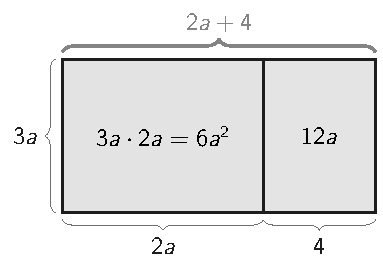
\includegraphics[width=0.95\linewidth]{expr_distributiva}
\end{minipage}
\begin{ojo}[Signos] $(+)(+) = +$, $(-)(-) = +$, $(+)(-) = -$. Así, $-2x(x - 4) = -2x^2 + 8x$. Y al multiplicar se suman exponentes: $x^2\cdot x^3 = x^5$, no $x^6$.\end{ojo}

\subsection{Del lenguaje natural al algebraico}
Lee la frase de afuera hacia adentro: la última operación que se nombra es la que manda. Si la edad de Pedro es $m$, «su edad hace $n$ años disminuida en 3» es $m - n - 3$; «el doble de la suma de un número y 5» es $2(x + 5)$, pero «el doble de un número, más 5» es $2x + 5$.
\begin{center}
\begin{tabular}{@{}ll@{\qquad}ll@{}}
\toprule
En palabras & Expresión & En palabras & Expresión\\ \midrule
el cuadrado de la suma de $a$ y $b$ & $(a + b)^2$ & el triple de la diferencia entre $x$ y 2 & $3(x - 2)$\\
la suma de los cuadrados & $a^2 + b^2$ & dos consecutivos & $n$ y $n + 1$\\
4 menos que $x$ & $x - 4$ & un número par & $2n$\\ \bottomrule
\end{tabular}
\end{center}

\subsection{Perímetros y áreas con expresiones}
Si un rectángulo mide $(2x + 3)$ por $(x - 1)$, su \textbf{perímetro} es $2(2x + 3) + 2(x - 1) = 6x + 4$ y su \textbf{área} es $(2x + 3)(x - 1) = 2x^2 + x - 3$. Con $x = 4$ mide 11 por 3: perímetro 28 y área 33, igual que con las expresiones.
\begin{ojo}[No confundas] El perímetro suma lados (no aparece $x^2$); el área los multiplica. Y para lo que sobra se resta \textbf{todo}, con paréntesis: $(10x + 8) - (6x + 4) = 4x + 4$.\end{ojo}
\gatotip[\gatonaranjo]{¿Dudas entre alternativas? Reemplaza la letra por un número sencillo, como 2, en el enunciado y en cada alternativa: la correcta da lo mismo.}

\begin{elejemplo}{PAES Regular 2026}
Una pista de baile de forma rectangular tiene dimensiones de $(3x + 4)$ metros de largo y $(2x - 9)$ metros de ancho. Se cuenta con $(20x + 20)$ metros de una cinta luminosa para demarcar el borde de la pista de baile.
\begin{center}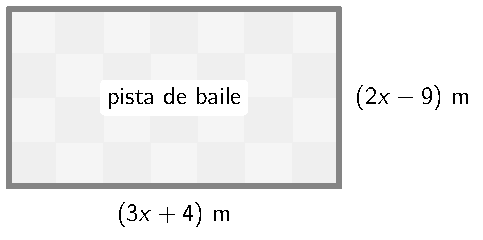
\includegraphics[width=5.2cm]{expr_pista}\end{center}
¿Cuántos metros de cinta luminosa sobran luego de demarcar el borde de la pista?
\alts{$(10x + 30)$ metros}{$(10x + 10)$ metros}{$(15x + 15)$ metros}{$(15x + 25)$ metros}
\solucion{Demarcar el borde es recorrer el perímetro: $2(3x + 4) + 2(2x - 9) = 6x + 8 + 4x - 18 = 10x - 10$. Lo que sobra es la cinta menos todo el perímetro:
\[ (20x + 20) - (10x - 10) = 20x + 20 - 10x + 10 = 10x + 30. \]
Comprobación con $x = 10$: la pista mide 34 m por 11 m, su perímetro es 90 m, la cinta mide 220 m y sobran 130 m $= 10\cdot 10 + 30$. $(10x + 10)$ cambia solo el primer signo del paréntesis; $(15x + 25)$ y $(15x + 15)$ restan medio perímetro.}{A}
\end{elejemplo}

%% =====================================================================
\section{Productos notables}

\subsection{Qué es un producto notable}
Son multiplicaciones tan frecuentes que conviene saber su resultado de memoria. Todas salen de multiplicar término a término, pero reconocer el molde ahorra tiempo y errores de signo.
\begin{clave}[Los cuatro moldes]
\[ (a + b)^2 = a^2 + 2ab + b^2 \qquad (a - b)^2 = a^2 - 2ab + b^2 \]
\[ (a + b)(a - b) = a^2 - b^2 \qquad (x + p)(x + q) = x^2 + (p + q)x + pq \]
Las letras son moldes: en $(2x + 5)^2$, $a = 2x$ y $b = 5$.\end{clave}

\subsection{Cuadrado de binomio}
\begin{minipage}[c]{0.62\linewidth}
En palabras: \textbf{el cuadrado del primero, más (o menos) el doble del primero por el segundo, más el cuadrado del segundo}. El dibujo lo muestra: el cuadrado de lado $a + b$ se parte en $a^2$, $b^2$ y \textbf{dos} rectángulos $ab$.
\[ (x + 5)^2 = x^2 + 10x + 25 \qquad (2x + 3)^2 = 4x^2 + 12x + 9 \]
\[ (x - 4)^2 = x^2 - 8x + 16 \qquad (3x - 2y)^2 = 9x^2 - 12xy + 4y^2 \]
En la resta, el término del medio es negativo y el último \textbf{siempre es positivo}. Además, $(a - b)^2 = (b - a)^2$.
\end{minipage}\hfill
\begin{minipage}[c]{0.34\linewidth}\centering
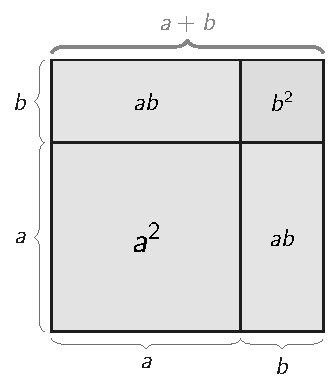
\includegraphics[width=0.85\linewidth]{expr_cuadrado_binomio}
\end{minipage}
\begin{ojo}[El error más común de la PAES] $(a + b)^2 \ne a^2 + b^2$: faltan los dos rectángulos. Con números, $(3 + 4)^2 = 49$, pero $3^2 + 4^2 = 25$. Revisa los tres términos: $(x - 4)^2$ no es $x^2 - 16$, ni $x^2 - 8x - 16$, ni $x^2 - 4x + 16$.\end{ojo}
\gatotip[\gatoatigrado]{Cálculo mental: $21^2 = (20 + 1)^2 = 400 + 40 + 1 = 441$ y $99^2 = (100 - 1)^2 = 10.000 - 200 + 1 = 9801$.}

\subsection{Suma por diferencia}
\begin{minipage}[c]{0.5\linewidth}
Al multiplicar, los términos del medio se cancelan: $(a + b)(a - b) = a^2 - ab + ab - b^2 = a^2 - b^2$. En el dibujo, a un cuadrado de lado $a$ se le quita uno de lado $b$ y lo que queda se reordena en un rectángulo de lados $a + b$ y $a - b$.

$(x + 7)(x - 7) = x^2 - 49$, \quad $(3x + 2y)(3x - 2y) = 9x^2 - 4y^2$ \quad y \quad $103\cdot 97 = 100^2 - 3^2 = 9991$.
\end{minipage}\hfill
\begin{minipage}[c]{0.46\linewidth}\centering
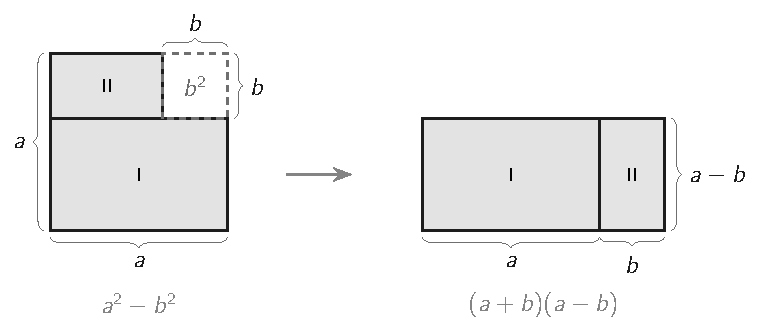
\includegraphics[width=\linewidth]{expr_suma_diferencia}
\end{minipage}
\begin{ojo}[Mismos términos, un signo distinto] $(x + 3)(x - 2)$ no es suma por diferencia.\end{ojo}

\subsection{Binomios con término común}
\begin{minipage}[c]{0.62\linewidth}
En $(x + p)(x + q)$ el resultado es $x^2$, más \textbf{la suma} de los números por $x$, más \textbf{su producto}. En el dibujo, $(x + 4)(x + 3) = x^2 + 7x + 12$.
\[ (x - 5)(x + 2) = x^2 - 3x - 10 \qquad (x - 2)(x - 6) = x^2 - 8x + 12 \]
Si $p = q$ es un cuadrado de binomio; si $q = -p$, una suma por diferencia.
\end{minipage}\hfill
\begin{minipage}[c]{0.34\linewidth}\centering
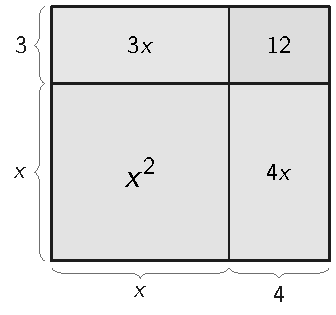
\includegraphics[width=0.8\linewidth]{expr_binomios_comun}
\end{minipage}

\subsection{Combinar productos notables}
Desarrolla cada producto por separado y \textbf{resta con paréntesis}:
\[ (x + 3)^2 - (x + 3)(x - 3) = (x^2 + 6x + 9) - (x^2 - 9) = x^2 + 6x + 9 - x^2 + 9 = 6x + 18. \]
\begin{ejemplo}[Usar datos sin despejar] Si $a + b = 7$ y $ab = 10$: $a^2 + b^2 = (a + b)^2 - 2ab = 49 - 20 = 29$, sin saber cuánto valen $a$ y $b$.\end{ejemplo}
\begin{ojo}[Errores típicos] $(2x)^2 = 4x^2$, no $2x^2$. $(x + 5)^2$ lleva $10x$, no $5x$. $(x + 4)(x - 4) = x^2 - 16$, no $x^2 + 16$. Y al restar $x^2 - 9$, el $-9$ se vuelve $+9$.\end{ojo}
\gatotip[\gatogris]{Comprueba con $x = 1$: la expresión original y tu resultado deben dar el mismo número.}

\begin{elejemplo}{PAES Invierno 2026}
¿Cuál de las siguientes expresiones es igual a $(2x - 3)^2 - (2x - 3)(2x + 3)$?
\alts{$18$}{$0$}{$-6x + 18$}{$-12x + 18$}
\solucion{Cuadrado de binomio con $a = 2x$ y $b = 3$: $(2x - 3)^2 = 4x^2 - 12x + 9$. Suma por diferencia: $(2x - 3)(2x + 3) = 4x^2 - 9$. Restando con paréntesis:
\[ (4x^2 - 12x + 9) - (4x^2 - 9) = 4x^2 - 12x + 9 - 4x^2 + 9 = -12x + 18. \]
Comprobación con $x = 1$: $1 - (-5) = 6$ y $-12 + 18 = 6$. El 18 olvida el término del medio, el 0 cree que los dos productos son iguales y $-6x + 18$ olvida el 2 del doble producto.}{D}
\end{elejemplo}

%% =====================================================================
\section{Factorización}

\subsection{Factorizar es deshacer la multiplicación}
\textbf{Factorizar} es escribir una suma como una multiplicación: el camino inverso de desarrollar. $3a(2a + 4) \to 6a^2 + 12a$ es desarrollar; $6a^2 + 12a \to 6a(a + 2)$ es factorizar. Con números ya lo haces: $12 + 20 = 4(3 + 5)$. Siempre se puede comprobar multiplicando.
\begin{ojo}[Factoriza completo] $3a(2a + 4)$ es igual a $6a^2 + 12a$, pero en el paréntesis queda un 2 común. La factorización completa saca el \textbf{mayor} factor común: $6a(a + 2)$.\end{ojo}

\subsection{Factor común}
\begin{clave}[Cómo encontrarlo] Números: su MCD. Letras: cada letra que está en \textbf{todos} los términos, con su \textbf{menor} exponente. Después divide cada término por el factor común.\end{clave}
\begin{ejemplo} $12x^3 - 18x^2$: MCD 6 y letra $x^2$, así que $12x^3 - 18x^2 = 6x^2(2x - 3)$. Si un término «desaparece» queda 1: $5x + 5 = 5(x + 1)$. El factor común puede ser un paréntesis: $x(a + b) + 3(a + b) = (a + b)(x + 3)$.\end{ejemplo}
\gatotip[\gatonegro]{Cálculo mental: $37\cdot 13 + 37\cdot 87 = 37(13 + 87) = 3700$. El 37 sale una sola vez.}

\subsection{Diferencia de cuadrados}
\begin{clave} \[ a^2 - b^2 = (a + b)(a - b) \] Dos cuadrados separados por un menos. Se usan sus \textbf{raíces}.\end{clave}
\begin{ejemplo} $x^2 - 49 = (x + 7)(x - 7)$; $9x^2 - 16y^2 = (3x + 4y)(3x - 4y)$; $2x^2 - 50 = 2(x^2 - 25) = 2(x + 5)(x - 5)$; $51^2 - 49^2 = 100\cdot 2 = 200$.\end{ejemplo}
\begin{ojo}[La suma de cuadrados no se factoriza así] $x^2 + 9$ no es $(x + 3)(x - 3)$, que da $x^2 - 9$, ni $(x + 3)^2$, que da $x^2 + 6x + 9$.\end{ojo}

\subsection{Trinomio cuadrado perfecto}
\begin{clave} \[ a^2 + 2ab + b^2 = (a + b)^2 \qquad a^2 - 2ab + b^2 = (a - b)^2 \] Los extremos son cuadrados positivos; saca sus raíces; el término del medio debe ser el \textbf{doble} de su producto, y su signo dice si es suma o resta.\end{clave}
\begin{ejemplo} $x^2 + 10x + 25$: raíces $x$ y 5, y $2\cdot x\cdot 5 = 10x$: es $(x + 5)^2$. $4x^2 - 12x + 9 = (2x - 3)^2$. En cambio, $x^2 + 6x + 25$ no es cuadrado perfecto: el medio debería ser $10x$.\end{ejemplo}

\subsection{Trinomio x² + bx + c}
\begin{minipage}[c]{0.64\linewidth}
\[ x^2 + bx + c = (x + p)(x + q) \quad\text{con}\quad p + q = b,\ \ pq = c \]
Busca \textbf{dos números que multiplicados den $c$ y sumados den $b$}. En $x^2 + 7x + 12$ son 3 y 4: $(x + 3)(x + 4)$, el rectángulo del dibujo.
\begin{clave}[Regla de signos] Si $c$ es positivo, los dos números tienen el signo de $b$: $x^2 - 9x + 20 = (x - 4)(x - 5)$. Si $c$ es negativo, tienen signos distintos: $x^2 - 2x - 15 = (x - 5)(x + 3)$.\end{clave}
\end{minipage}\hfill
\begin{minipage}[c]{0.32\linewidth}\centering
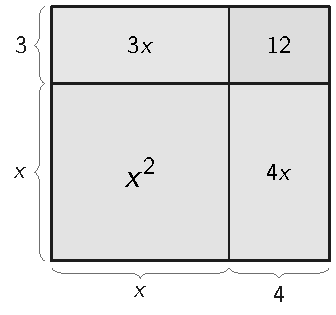
\includegraphics[width=0.85\linewidth]{expr_binomios_comun}
\end{minipage}

\subsection{Simplificar fracciones algebraicas}
Solo se tachan \textbf{factores} (cosas que multiplican), nunca sumandos. Por eso primero se factoriza:
\[ \frac{x^2 - 9}{x + 3} = \frac{(x + 3)(x - 3)}{x + 3} = x - 3 \ \ (x \ne -3), \qquad \frac{x^2 + 5x}{x^2 - 25} = \frac{x(x + 5)}{(x + 5)(x - 5)} = \frac{x}{x - 5}. \]
El valor que anula el denominador original queda excluido también después de simplificar.
\begin{ojo}[Así no] $\dfrac{x + 6}{x + 2} \ne \dfrac{6}{2}$. Con $x = 2$ vale $\dfrac{8}{4} = 2$, no 3.\end{ojo}

\subsection{Qué factorización uso}
\begin{center}
\small\begin{tabular}{@{}lll@{}}
\toprule
Mira esto & Usa & Ejemplo\\ \midrule
algo se repite en todos los términos & factor común (siempre primero) & $4x^2 + 6x = 2x(2x + 3)$\\
dos cuadrados con un menos & diferencia de cuadrados & $x^2 - 36 = (x + 6)(x - 6)$\\
extremos cuadrados y medio $2ab$ & trinomio cuadrado perfecto & $x^2 - 8x + 16 = (x - 4)^2$\\
$x^2 + bx + c$ & producto $c$, suma $b$ & $x^2 + x - 12 = (x + 4)(x - 3)$\\ \bottomrule
\end{tabular}
\end{center}
Después revisa si algún paréntesis se puede factorizar de nuevo: $3x^2 - 12 = 3(x + 2)(x - 2)$ y $2x^3 - 8x^2 + 8x = 2x(x - 2)^2$. Si un producto vale 0, algún factor vale 0: $(p - 3)^2 - 36 = (p + 3)(p - 9) = 0$ da $p = -3$ o $p = 9$.
\gatotip[\gatolila]{Con un área y un lado, factoriza el área: si mide $x^2 + 7x + 12$ y un lado es $x + 3$, el otro es $x + 4$. Y descarta las medidas negativas.}

\begin{elejemplo}{PAES Regular 2026, adaptada}
Una persona realiza el siguiente procedimiento para factorizar $12x^2 + 20x$, cometiendo un error.

Paso 1: escribe cada término como un producto, obteniendo $4\cdot 3\cdot x\cdot x + 4\cdot 5\cdot x$.\\
Paso 2: descompone cada número en factores primos, obteniendo $2\cdot 2\cdot 3\cdot x\cdot x + 2\cdot 2\cdot 5\cdot x$.\\
Paso 3: escribe las potencias correspondientes, obteniendo $2^2\cdot 3\cdot x^2 + 2^2\cdot 5\cdot x$.\\
Paso 4: factoriza la suma, obteniendo $2^4x(3x + 5)$.

¿En cuál de los pasos la persona cometió el error?
\alts{En el Paso 1}{En el Paso 2}{En el Paso 3}{En el Paso 4}
\solucion{Los Pasos 1, 2 y 3 solo reescriben los números: cada expresión sigue siendo igual a $12x^2 + 20x$. En el Paso 4, el factor común es lo que se repite en los dos términos, $2^2$ y $x$, o sea $4x$; la persona sumó los exponentes de los dos $2^2$ y escribió $2^4 = 16$. Lo que se repite se saca \textbf{una vez}. Lo correcto es $12x^2 + 20x = 4x(3x + 5)$; en cambio, $2^4x(3x + 5) = 48x^2 + 80x$, el cuádruple de lo pedido.}{D}
\end{elejemplo}

%% =====================================================================
\section{Proporcionalidad directa}

\subsection{Razón y proporción}
Una \textbf{razón} compara dos cantidades dividiéndolas: 12 niñas y 18 niños están en la razón $12 : 18 = \frac{12}{18} = 2 : 3$, es decir, por cada 2 niñas hay 3 niños. Una \textbf{proporción} es una igualdad de razones, como $\frac{2}{3} = \frac{8}{12}$.
\begin{clave}[Propiedad fundamental] $\dfrac{a}{b} = \dfrac{c}{d}$ es lo mismo que $a\cdot d = b\cdot c$ (producto cruzado). Con ella se despeja el término que falta: $\dfrac{x}{15} = \dfrac{2}{3} \Rightarrow 3x = 30 \Rightarrow x = 10$.\end{clave}
\begin{ojo}[El orden importa] Cuando dice \textbf{respectivamente}, el primer número va con lo primero que se nombra. Y si la razón es $2 : 3$, el grupo tiene $2 + 3 = 5$ partes: las niñas son $\frac{2}{5}$ del curso, no $\frac{2}{3}$.\end{ojo}

\subsection{Qué es la proporcionalidad directa}
Dos cantidades son \textbf{directamente proporcionales} si, cuando una se multiplica por un número, la otra se multiplica por el \textbf{mismo} número: el doble con el doble, la mitad con la mitad. El cociente es constante:
\begin{clave} \[ \frac{y}{x} = k \qquad\Longleftrightarrow\qquad y = k\cdot x \] La constante $k$ es lo que vale $y$ cuando $x = 1$: el precio de \textbf{un} cuaderno, lo que se paga por \textbf{un} minuto. Se llama valor unitario.\end{clave}
\begin{center}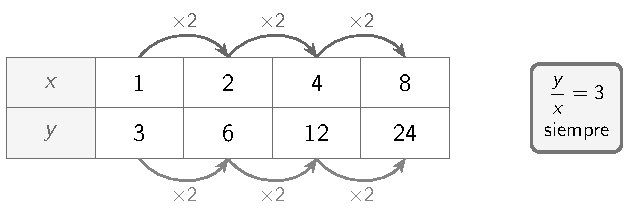
\includegraphics[width=8.2cm]{prop_tabla_directa}\end{center}
\textbf{En una tabla}, divide $y$ por $x$ en cada columna: con $x$: 2, 5, 8 e $y$: 6, 15, 24 siempre da 3, así que es directa. Con $x$: 1, 2, 3 e $y$: 5, 7, 9 da 5; 3,5 y 3: no lo es (es $y = 2x + 3$).
\begin{ojo}[Que las dos crezcan no basta] Al pasar de $x = 1$ a $x = 2$, $y$ debe duplicarse. Además, si $x = 0$, entonces $y = 0$: con un cobro fijo (la bajada de bandera de un taxi) ya no es proporcional.\end{ojo}

\subsection{El gráfico: una recta que pasa por el origen}
\begin{minipage}[c]{0.5\linewidth}
Los puntos $(x, y)$ de $y = kx$ quedan sobre una recta que pasa por $(0, 0)$. Para leer $k$, toma un punto distinto del origen y divide su altura por su $x$: con $(4, 12)$, $k = 3$. Cada vez que avanzas 1, la recta sube $k$: $k$ es la pendiente.

En cambio, $y = 3x + 2$ también es una recta, pero corta el eje $Y$ en 2: no es proporcionalidad directa.
\end{minipage}\hfill
\begin{minipage}[c]{0.46\linewidth}\centering
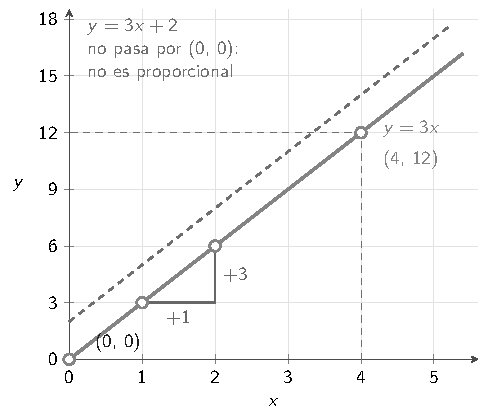
\includegraphics[width=0.92\linewidth]{prop_graf_directa}
\end{minipage}

\subsection{La regla de tres directa}
\begin{ejemplo} 4 kg de paltas cuestan \peso 7200; ¿cuánto cuestan 6 kg? \textbf{Valor unitario:} 1 kg cuesta $\frac{7200}{4} = 1800$, y 6 kg, $6\cdot 1800 = 10.800$. \textbf{Proporción:} $\frac{4}{7200} = \frac{6}{x}$, así que $4x = 43.200$ y $x = 10.800$.\end{ejemplo}
\begin{ojo}[Revisa el sentido] Kilos arriba y pesos abajo en las dos razones. Si te da que 6 kg cuestan menos que 4 kg, armaste mal la proporción. Y si una cantidad aumenta en 100, la otra no aumenta en 100: aumenta en la misma \textbf{proporción}.\end{ojo}
\gatotip[\gatoblanco]{Las escalas de mapas son proporción directa: si 1 cm equivale a 50 m, 7 cm son $7\cdot 50 = 350$ m. Calcula primero lo que vale 1 cm.}

\subsection{Repartos proporcionales}
\begin{clave}[Repartir en la razón $a : b$] Cuenta las partes, $a + b$; divide el total por ese número para obtener una parte, y multiplica por las partes de cada uno.\end{clave}
\begin{ejemplo} \peso 60.000 en la razón $2 : 3$: son 5 partes de 12.000; Ana recibe 24.000 y Beto 36.000. Si se reparte según lo que aportó cada uno (\peso 3000 y \peso 2000), la razón es $3 : 2$.\end{ejemplo}
\begin{ojo}[No dividas por 2] Repartir en la razón $2 : 3$ no es repartir por mitades, ni dividir por 2 y por 3: se divide por el total de partes, 5.\end{ojo}

\begin{elejemplo}{PAES Invierno 2026, adaptada}
Javier y David compraron una bolsa de 24 dulces a un precio total de \peso 2100, tal que Javier aportó \peso 1400 y David aportó el resto del dinero.

Ellos deciden vender cada dulce a \peso 200 y repartirse el dinero obtenido de forma proporcional a lo que aportó cada uno en la compra.

¿Cuánto dinero recibirá Javier luego de vender todos los dulces?
\alts{\peso 1600}{\peso 2400}{\peso 2700}{\peso 3200}
\solucion{La venta da $24\cdot 200 = 4800$ pesos. David aportó $2100 - 1400 = 700$, así que los aportes están en la razón $1400 : 700 = 2 : 1$. Son $2 + 1 = 3$ partes de $\frac{4800}{3} = 1600$, y Javier recibe 2 partes: $3200$ pesos. Comprobación: David recibe 1600 y $3200 + 1600 = 4800$. \peso 1600 es lo de David, \peso 2400 reparte por mitades y \peso 2700 es la ganancia total.}{D}
\end{elejemplo}

%% =====================================================================
\section{Proporcionalidad inversa}

\subsection{Qué es la proporcionalidad inversa}
Dos cantidades son \textbf{inversamente proporcionales} si, cuando una se multiplica por un número, la otra se \textbf{divide} por ese mismo número: si una se duplica, la otra se reduce a la mitad. Al repartir 24 caramelos entre 1, 2, 4 u 8 niños tocan 24, 12, 6 o 3: el producto siempre es 24.
\begin{clave} \[ x\cdot y = k \qquad\Longleftrightarrow\qquad y = \frac{k}{x} \] La constante $k$ es el total: lo que se reparte, la distancia del viaje, el trabajo de la obra.\end{clave}
\begin{center}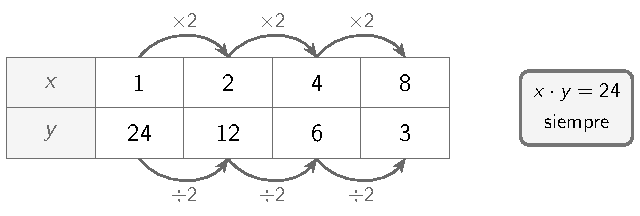
\includegraphics[width=8.2cm]{prop_tabla_inversa}\end{center}

\subsection{Cómo reconocerla}
En una tabla, \textbf{multiplica} $x$ por $y$ en cada columna. A 60 km/h se tarda 4 h, a 80 km/h 3 h y a 120 km/h 2 h: el producto es siempre 240 (la distancia), así que es inversa. Con $x$: 1, 2, 3 e $y$: 10, 8, 6 los productos son 10, 16 y 18: no lo es.
\begin{center}
\begin{tabular}{@{}lll@{}}
\toprule
 & Directa & Inversa\\ \midrule
lo constante & $\dfrac{y}{x} = k$ & $x\cdot y = k$\\[6pt]
fórmula & $y = kx$ & $y = \dfrac{k}{x}$\\[6pt]
si $x$ se duplica & $y$ se duplica & $y$ se divide por 2\\
gráfico & recta por el origen & hipérbola\\ \bottomrule
\end{tabular}
\end{center}
\begin{ojo}[Que una baje cuando la otra sube no basta] En $y = 10 - x$, $y$ baja, pero $1\cdot 9 = 9$ y $2\cdot 8 = 16$. Revisa \textbf{todas} las columnas.\end{ojo}

\subsection{El gráfico: una hipérbola}
\begin{minipage}[c]{0.5\linewidth}
Los puntos de $y = \frac{24}{x}$ forman una curva llamada \textbf{hipérbola}: cuando $x$ crece, $y$ baja, primero rápido y después cada vez más lento. Se acerca a los ejes pero \textbf{nunca los toca}, porque $x$ e $y$ no pueden valer 0.

Desde el origen hasta cada punto se forma un rectángulo de área $x\cdot y = 24$: todos tienen la misma área.
\end{minipage}\hfill
\begin{minipage}[c]{0.46\linewidth}\centering
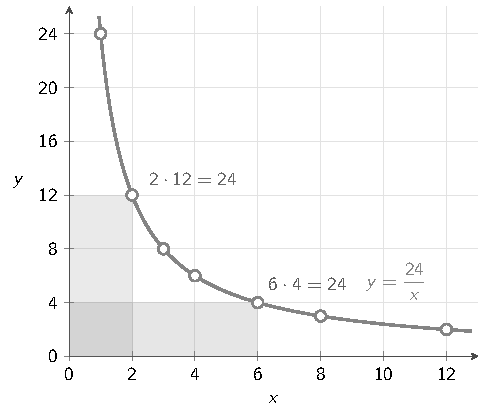
\includegraphics[width=0.92\linewidth]{prop_graf_inversa}
\end{minipage}

\subsection{Trabajadores, rapidez, raciones y llaves}
\begin{clave}[Método] 1. ¿Más de una da menos de la otra? 2. Calcula $k = x\cdot y$, el total. 3. Divide $k$ por la nueva cantidad. 4. Revisa el sentido.\end{clave}
\begin{ejemplo}[Trabajadores] 6 obreros tardan 10 días: la obra son $6\cdot 10 = 60$ «días de un obrero». Con 4 obreros: $\frac{60}{4} = 15$ días. Con proporción, sin dar vuelta nada: $6\cdot 10 = 4\cdot x$.\end{ejemplo}
\begin{ejemplo}[Rapidez, raciones y llaves] A 90 km/h se tarda 4 h: son 360 km, y a 120 km/h se tarda 3 h. Comida para 20 personas por 15 días son 300 raciones: con 25 personas alcanza para 12 días. 3 llaves llenan un estanque en 8 h: son 24 «horas de una llave», y con 4 llaves se tarda 6 h.\end{ejemplo}
\begin{ojo}[El error más común] Hacer regla de tres directa: $\frac{6}{10} = \frac{4}{x}$ da 6,7 días, como si con menos obreros se terminara antes. Todo esto supone el mismo ritmo, que la PAES indica con frases como «en las mismas condiciones».\end{ojo}

\subsection{Dos proporciones a la vez}
Si cambian tres cantidades, ve al \textbf{valor de una unidad}. 4 trabajadores llenan 2000 cajas en 20 días: los 4 llenan $\frac{2000}{20} = 100$ cajas diarias y uno solo, $\frac{100}{4} = 25$. Para 32.000 cajas en 10 días se necesitan 3200 diarias, o sea $\frac{3200}{25} = 128$ trabajadores.
\gatotip[\gatonaranjo]{Lo que hace \emph{uno} se obtiene \emph{dividiendo} lo que hacen todos. Un solo trabajador no puede llenar más cajas que los cuatro juntos.}

\subsection{Directa, inversa o ninguna}
\begin{center}
\begin{tabular}{@{}lll@{}}
\toprule
Situación & Al duplicar $x$ & Tipo\\ \midrule
kilos de pan y precio a pagar & el precio se duplica & directa\\
rapidez y tiempo de un mismo viaje & el tiempo se reduce a la mitad & inversa\\
personas y porción de una torta & la porción se reduce a la mitad & inversa\\
minutos y cobro con cargo fijo & aumenta, pero no al doble & ninguna\\
edad y estatura & no hay regla fija & ninguna\\ \bottomrule
\end{tabular}
\end{center}
\gatotip[\gatogris]{$k$ no es la respuesta: si $x\cdot y = 60$ y $x = 5$, la respuesta es $y = 12$, no 60.}

\begin{elejemplo}{PAES Invierno 2027, adaptada}
En una empresa hay 4 trabajadores para cosechar uvas y estos logran llenar 2000 cajas en 20 días de trabajo, todos trabajando todos los días, al mismo ritmo y la misma cantidad de horas.

En la empresa se realiza el siguiente procedimiento para calcular la cantidad de trabajadores necesarios para llenar 32.000 cajas en 10 días, bajo las mismas condiciones, cometiéndose un error.

Paso 1: se calcula la cantidad de cajas que llenan diariamente los 4 trabajadores en conjunto como $\frac{2000}{20}$, obteniéndose que llenan 100 cajas diarias.\\
Paso 2: se calcula la cantidad de cajas que cada trabajador llena diariamente como $100\cdot 4$, obteniéndose 400 cajas diarias por trabajador.\\
Paso 3: se calcula la cantidad de cajas que se deben llenar diariamente para la nueva producción como $\frac{32.000}{10}$, obteniéndose 3200 cajas diarias.\\
Paso 4: se divide la cantidad de cajas diarias que se deben llenar por la cantidad que cada trabajador llena diariamente como $\frac{3200}{400}$, obteniéndose que se necesitan 8 trabajadores.

¿En cuál de los pasos se cometió el error?
\alts{En el Paso 1}{En el Paso 2}{En el Paso 3}{En el Paso 4}
\solucion{El Paso 1 está bien: $\frac{2000}{20} = 100$ cajas diarias entre los 4. En el Paso 2 está el error: lo que llena \textbf{uno} es $\frac{100}{4} = 25$ cajas diarias; se multiplicó por 4 en vez de dividir. El Paso 3 está bien ($\frac{32.000}{10} = 3200$) y el Paso 4 tiene la idea correcta, pero arrastra el 400. Lo correcto: $\frac{3200}{25} = 128$ trabajadores, que llenan $128\cdot 25 = 3200$ cajas diarias.}{B}
\end{elejemplo}

%% =====================================================================
\section{Sistemas de ecuaciones lineales}

\subsection{Qué es un sistema de ecuaciones}
Un \textbf{sistema} son dos ecuaciones con las mismas dos incógnitas que se deben cumplir \textbf{al mismo tiempo}. Su \textbf{solución} es el par $(x, y)$ que hace verdaderas \textbf{las dos}:
\[ \begin{cases} x + y = 10 \\ x - y = 4 \end{cases} \qquad\text{solución } (7, 3):\quad 7 + 3 = 10,\ \ 7 - 3 = 4. \]
\begin{ojo}[Las dos, no una] $(6, 4)$ cumple la primera, pero no la segunda: no es solución. Y en el par va primero la $x$: $(3, 7)$ es otro par.\end{ojo}

\subsection{Los tres métodos}
\begin{clave}[Sustitución] Despeja una incógnita y \textbf{reemplázala con paréntesis} en la otra ecuación. Conviene cuando una letra tiene coeficiente 1 o $-1$.\end{clave}
\begin{ejemplo} $2x + y = 11$ y $x - 3y = -5$: $y = 11 - 2x$, y $x - 3(11 - 2x) = -5$ da $7x - 33 = -5$, o sea $x = 4$ e $y = 3$.\end{ejemplo}
\begin{clave}[Igualación] Despeja la misma incógnita en las dos e iguala. Conviene cuando las dos vienen como $y = \dots$\end{clave}
\begin{ejemplo} $y = 2x + 1$ e $y = -x + 7$: $2x + 1 = -x + 7$, así que $x = 2$ e $y = 5$.\end{ejemplo}
\begin{clave}[Reducción] Suma las ecuaciones para que una incógnita desaparezca; si hace falta, antes multiplica \textbf{toda} una ecuación. Conviene con coeficientes opuestos.\end{clave}
\begin{ejemplo} $2x + 3y = 12$ y $3x - y = 7$: la segunda por 3 es $9x - 3y = 21$; sumando, $11x = 33$, $x = 3$ e $y = 2$.\end{ejemplo}
\begin{ojo}[Errores típicos] Reemplazar sin paréntesis ($x - 3\cdot 11 - 2x$); multiplicar solo un lado ($9x - 3y = 7$); quedarse con una incógnita o dar vuelta el par. Con fracciones, multiplica antes la ecuación por el mcm.\end{ojo}
\gatotip[\gatoatigrado]{Si te quedas en blanco, reemplaza cada alternativa en las \emph{dos} ecuaciones: la correcta cumple ambas. Y si te dan la solución con letras $a$ y $b$, reemplázala para encontrarlas.}

\subsection{Una, ninguna o infinitas soluciones}
Cada ecuación lineal es una \textbf{recta} y la solución del sistema es el punto donde se cortan (por ejemplo, $x + y = 5$ y $x - y = 1$ se cortan en $(3, 2)$). Dos rectas pueden estar de tres maneras:
\begin{center}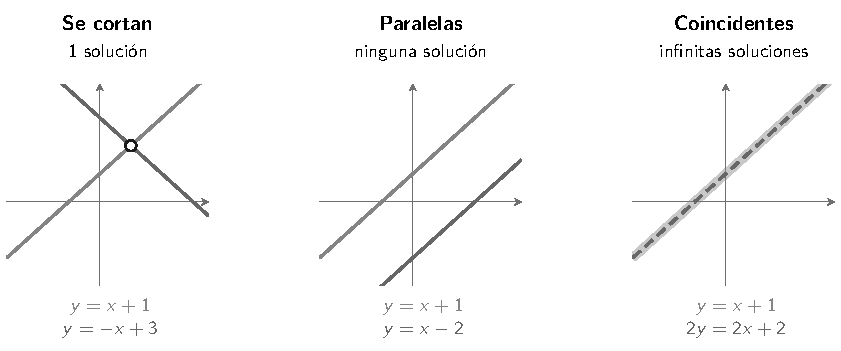
\includegraphics[width=0.85\linewidth]{sis_tres_casos}\end{center}
\begin{center}
\begin{tabular}{@{}llll@{}}
\toprule
Rectas & Despejando $y$ & Soluciones & Al resolver queda\\ \midrule
se cortan & distinta pendiente & una & $x$ e $y$\\
paralelas & misma pendiente, distinto corte & ninguna & algo falso, como $0 = -2$\\
coincidentes & todo igual & infinitas & $0 = 0$\\ \bottomrule
\end{tabular}
\end{center}
\begin{ejemplo} $x + 2y = 3$ y $x + 2y = 5$ son paralelas. $x + 2y = 3$ y $2x + 4y = 6$ son la misma recta: la segunda es la primera multiplicada por 2 en \textbf{todos} sus términos.\end{ejemplo}
\begin{ojo}[Nunca dos] Dos rectas distintas no se cortan en exactamente dos puntos.\end{ojo}

\begin{elejemplo}{Tipo PAES}
¿Cuál es la solución del siguiente sistema de ecuaciones?
\[ \begin{cases} 3x - 2y = 5 \\ x + 4y = 11 \end{cases} \]
\alts{$(2, 3)$}{$(1, -1)$}{$(3, 2)$}{$(7, 1)$}
\solucion{En la segunda la $x$ tiene coeficiente 1: sustitución. $x = 11 - 4y$, y en la primera, $3(11 - 4y) - 2y = 5$, o sea $33 - 14y = 5$, $-14y = -28$ e $y = 2$. Entonces $x = 11 - 8 = 3$. Comprobación: $9 - 4 = 5$ y $3 + 8 = 11$. $(2, 3)$ da vuelta el par, $(1, -1)$ solo cumple la primera y $(7, 1)$ solo la segunda.}{C}
\end{elejemplo}

%% =====================================================================
\section{Problemas con sistemas de ecuaciones}

\subsection{Del enunciado al sistema en 4 pasos}
\begin{clave}[Los 4 pasos] 1. Nombra las dos incógnitas, con su unidad. 2. Escribe una ecuación por cada dato total: casi siempre uno de \textbf{cantidades} y otro de \textbf{valor}. 3. Resuelve. 4. Responde y comprueba en el enunciado.\end{clave}
\begin{ejemplo}[Entradas] Adulto \peso 5000, niño \peso 3000; 80 entradas y \peso 300.000: $x + y = 80$ y $5000x + 3000y = 300.000$. Con $y = 80 - x$ se llega a $2000x = 60.000$: 30 de adulto y 50 de niño.\end{ejemplo}
\begin{ojo}[No mezcles] En la ecuación de cantidades no van precios, y en la de dinero cada cantidad va con \textbf{su} precio. $x + y = 300.000$ no tiene sentido: suma entradas y da pesos.\end{ojo}

\subsection{Monedas, edades y mezclas}
\begin{ejemplo}[Monedas] 30 monedas de \peso 100 y \peso 500 suman \peso 7400: $x + y = 30$ y $100x + 500y = 7400$. Dividiendo la segunda por 100, $x + 5y = 74$; restando la primera, $4y = 44$: 11 de 500 y 19 de 100.\end{ejemplo}
\begin{ejemplo}[Edades] Padre e hijo suman 50; hace 5 años el padre tenía 4 veces la edad del hijo: $p + h = 50$ y $p - 5 = 4(h - 5)$. Resulta $h = 13$ y $p = 37$.\end{ejemplo}
\begin{ojo}[Paréntesis en las edades] «4 veces la edad del hijo hace 5 años» es $4(h - 5)$, no $4h - 5$. Y el tiempo pasa para todos: en 4 años, $a + 4 = 3(h + 4)$.\end{ojo}
\begin{ejemplo}[Mezclas] Café de \peso 8000 y de \peso 12.000 el kilo para 20 kg a \peso 9000: $x + y = 20$ y $8000x + 12.000y = 20\cdot 9000$. Resulta 15 kg del barato y 5 kg del caro: el precio de la mezcla está más cerca del café barato.\end{ejemplo}
\gatotip[\gatolila]{Si el precio es «por kilogramo», la incógnita son \emph{kilogramos}, no frutas ni paquetes. La PAES pregunta justo eso.}

\subsection{Planes: ¿cuándo cuestan lo mismo?}
\begin{minipage}[c]{0.5\linewidth}
Plan A: \peso 8000 más \peso 50 por minuto; plan B: \peso 12.000 más \peso 30. Igualando, $8000 + 50m = 12.000 + 30m$: $m = 200$ minutos, con un costo de \peso 18.000 en ambos.

El punto donde se cortan las rectas es donde las dos cantidades valen lo mismo. Antes de 200 minutos conviene A; después, B.
\end{minipage}\hfill
\begin{minipage}[c]{0.46\linewidth}\centering
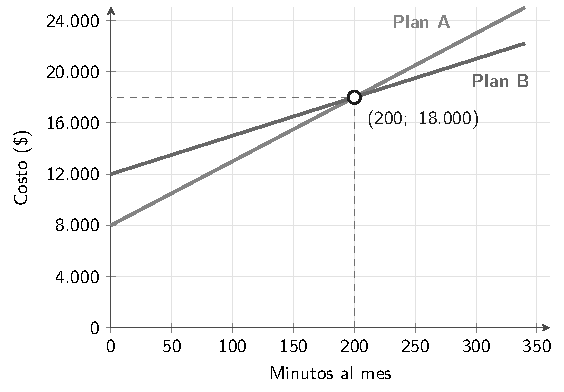
\includegraphics[width=\linewidth]{sis_planes}
\end{minipage}
\begin{ejemplo}[Tarifa fija] Con \peso 2300 por 40 minutos y \peso 3800 por 70: $f + 40v = 2300$ y $f + 70v = 3800$. Restando, $30v = 1500$: $v = 50$ y la tarifa fija es $f = 300$.\end{ejemplo}

\subsection{Qué representa cada parte del sistema}
En una obra de teatro la entrada de niño cuesta \peso 2000 y la de adulto \peso 3500; una familia pagó \peso 40.000 por 14 entradas:
\[ \begin{cases} x + y = 14 \\ 2000x + 3500y = 40.000 \end{cases} \]
\begin{clave}[Cantidad, precio o dinero] $x$ va con 2000: es la \textbf{cantidad} de entradas de niño. 2000 es un \textbf{precio}. $2000x$ es \textbf{dinero}: lo pagado por las entradas de niño. 40.000 es el total pagado y 14 el total de entradas.\end{clave}
\begin{ojo}[Porcentajes] Si aparece $\frac{80}{100}\cdot B$ como lo pagado con un 20~\% de descuento, $B$ es el precio \textbf{original}. Y no sumes lo que el enunciado excluye: «se recaudó solo por las poleras» deja fuera los envíos.\end{ojo}
\gatotip[\gatonegro]{Al final, relee qué representa cada letra: si piden las entradas de niño y respondes $y$, marcaste la otra.}

\begin{elejemplo}{PAES Invierno 2026, adaptada}
Una empresa dedicada a la venta de poleras ofrece a sus clientes dos opciones de diseño: personalizado o de catálogo. El precio por polera con diseño personalizado es \peso 8500 y con diseño de catálogo es \peso 7500. Adicionalmente, se hace un cobro por envío a domicilio de \peso 2500.

En un día de trabajo se vendió un total de 18 poleras en diez envíos y se recaudó \peso 146.000 solo por las poleras. Para calcular la cantidad de poleras con diseño personalizado que se vendieron, una persona realiza el siguiente procedimiento, cometiendo un error.

Paso 1: representa con $x$ la cantidad de poleras con diseño personalizado y con $y$ la cantidad de poleras con diseño de catálogo, y establece el sistema $\begin{cases} x + y = 18 \\ 8500x + 7500y = 146.000 + 25.000 \end{cases}$\\[2pt]
Paso 2: despeja $y$ de la primera ecuación, obteniendo $y = 18 - x$.\\
Paso 3: reemplaza $y$ en la segunda ecuación, obteniendo $8500x - 7500x = 146.000 + 25.000 - 7500\cdot 18$.\\
Paso 4: resuelve la igualdad anterior y determina que la cantidad de poleras con diseño personalizado es 36.

¿En cuál de los pasos la persona cometió el error?
\alts{En el Paso 1}{En el Paso 2}{En el Paso 3}{En el Paso 4}
\solucion{La primera ecuación está bien, pero en la segunda $8500x + 7500y$ es el dinero de las poleras, y el enunciado dice que se recaudaron 146.000 \textbf{solo por las poleras}: los $10\cdot 2500 = 25.000$ de los envíos no van ahí. El error está en el Paso 1. Los Pasos 2, 3 y 4 operan bien con lo que reciben. Lo correcto: $1000x = 146.000 - 135.000 = 11.000$, o sea 11 personalizadas y 7 de catálogo; $8500\cdot 11 + 7500\cdot 7 = 146.000$. Además, 36 poleras personalizadas es imposible si en total se vendieron 18.}{A}
\end{elejemplo}

\chapter{Funciones}
%% Estilo común de los gráficos del capítulo (rectas y parábolas pequeñas).
\pgfplotsset{capfun/.style={width=6.4cm,height=5cm,axis lines=middle,xlabel={$x$},ylabel={$y$},
  every axis x label/.style={at={(ticklabel* cs:1)},anchor=west,font=\small},
  every axis y label/.style={at={(ticklabel* cs:1)},anchor=south,font=\small},
  tick label style={font=\scriptsize},grid=major,grid style={gris!20},samples=120,
  every axis plot/.append style={line width=1.1pt}}}

%% =====================================================================
\section{Concepto de función}
%% =====================================================================

\subsection{Qué es una función}
Una \textbf{función} es una regla que a cada número que entra le asigna \textbf{un solo} número que sale. Al que entra lo llamamos $x$ y al que sale, $f(x)$ («f de x»).
\begin{itemize}
  \item \textbf{Variable independiente}: la $x$, lo que tú eliges.
  \item \textbf{Variable dependiente}: $y = f(x)$, lo que sale; depende de la $x$.
  \item \textbf{Dominio}: los valores que puede tomar la $x$. Si no se dice nada, son todos los números reales.
\end{itemize}
\begin{ejemplo} El kilo de pan cuesta \peso 2.000. Si compro $x$ kilos, pago $f(x) = 2.000\cdot x$. Con 2 kilos: $f(2) = 2.000\cdot 2 = 4.000$ pesos.\end{ejemplo}
\begin{ojo}[Ojo con la escritura] $f(2)$ no es «f por 2»: es lo que sale cuando entra el 2.\end{ojo}

\subsection{Una sola salida para cada entrada}
Un par $(x, y)$ dice «entra $x$, sale $y$». Para que un conjunto de pares sea función, ninguna $x$ puede tener dos salidas distintas.
\begin{clave}[La regla de oro] Dos entradas con la misma salida, como $(1, 5)$ y $(2, 5)$: \textbf{permitido}. Una entrada con dos salidas, como $(1, 5)$ y $(1, 7)$: \textbf{no es función}.\end{clave}
\begin{ejemplo} En $\{(2, 3),\ (5, 3),\ (2, 8)\}$ la entrada $2$ sale una vez $3$ y otra vez $8$: no es función.\end{ejemplo}
En un gráfico se usa una \textbf{recta vertical}: si en algún lugar corta la curva en dos puntos o más, no es función. Una recta horizontal sí puede cortarla varias veces.

\subsection{Evaluar: reemplazar la x}
Evaluar es cambiar \textbf{cada} $x$ de la fórmula por el número, \textbf{entre paréntesis}, y calcular respetando el orden: potencias, multiplicaciones, sumas.
\begin{ejemplo} Si $f(x) = 2x^2 - 7x + 1$:
$f(-3) = 2(-3)^2 - 7(-3) + 1 = 2\cdot 9 + 21 + 1 = 40$.\end{ejemplo}
\begin{ojo}[Tres trampas]
\begin{itemize}
  \item $(-3)^2 = 9$, pero $-3^2 = -(3\cdot 3) = -9$.
  \item $-x^2$ significa $-(x^2)$: si $g(x) = -x^2 + 10$, entonces $g(-3) = -9 + 10 = 1$, no $19$.
  \item $f(2) + f(3)$ no es $f(5)$: con $f(x) = 4x - 1$, $f(2) + f(3) = 7 + 11 = 18$, pero $f(5) = 19$.
\end{itemize}
\end{ojo}
\gatotip[\gatogris]{Reemplaza siempre con paréntesis, aunque el número sea positivo. Con los negativos es lo que te salva: menos por menos da más.}

\subsection{Imagen y preimagen}
Si $f(a) = b$, decimos que $b$ es la \textbf{imagen} de $a$ y que $a$ es una \textbf{preimagen} de $b$.
\begin{clave}[¿Evaluar o despejar?] Si te dan la $x$, \textbf{evalúa}. Si te dan el resultado, \textbf{iguala} la fórmula a ese resultado y despeja la $x$.\end{clave}
\begin{ejemplo} Si $g(x) = 4x + 6$, la preimagen de $26$ sale de $4x + 6 = 26$: $4x = 20$ y $x = 5$. Comprobación: $g(5) = 26$ \checkmark.\end{ejemplo}
Un número puede tener dos preimágenes o ninguna: si $h(x) = x^2$, el $9$ tiene dos ($3$ y $-3$), y el $-4$ no tiene ninguna, porque un cuadrado nunca es negativo. Si en la fórmula falta una constante, un dato como $f(2) = 11$ se convierte en una ecuación para encontrarla.

\subsection{Funciones en tablas y gráficos}
En una tabla, cada fila es un par (entrada, salida). Una fórmula corresponde a la tabla solo si calza en \textbf{todas} las filas. Si la $x$ sube de 1 en 1 y $f(x)$ sube siempre lo mismo, prueba «salto por $x$ más el valor en $x = 0$».

En un gráfico, la entrada se lee en el eje $X$ y la salida es la \textbf{altura}:
\begin{itemize}
  \item $f(a)$: desde $x = a$ sube (o baja) hasta la curva y lee la altura.
  \item $f(x) = b$: traza una horizontal a altura $b$ y, desde cada corte, baja a leer la $x$.
\end{itemize}
\begin{center}
\begin{tikzpicture}
\begin{axis}[capfun,xmin=-3,xmax=3,ymin=-1,ymax=9,xtick={-3,...,3},ytick={0,2,...,8}]
  \addplot[nar,domain=-3:3] {x^2};
  \addplot[azul,dashed,line width=0.8pt,domain=-3:3] {4};
  \draw[menta,dashed,line width=0.8pt] (axis cs:2,0) -- (axis cs:2,4);
  \addplot[only marks,mark=*,mark size=2pt,nard] coordinates {(2,4) (-2,4)};
  \node[font=\scriptsize,anchor=west] at (axis cs:2.05,3.4) {$(2, 4)$};
  \node[font=\scriptsize,anchor=east] at (axis cs:-2.05,3.4) {$(-2, 4)$};
\end{axis}
\end{tikzpicture}
\end{center}
\begin{ejemplo} En el gráfico de $f(x) = x^2$: desde $x = 2$ subo hasta la curva y la altura es $4$, así que $f(2) = 4$. La horizontal a altura $4$ corta la curva en $x = -2$ y $x = 2$: esas son las soluciones de $f(x) = 4$.\end{ejemplo}
\begin{ojo}[Gráficos en contexto] En un gráfico distancia-tiempo, un tramo que sube es avanzar y un tramo \textbf{plano} es estar detenido. Lo que dura la detención se lee restando en el eje del tiempo.\end{ojo}
\gatotip[\gatoatigrado]{Al final, reemplaza tu respuesta en la fórmula. Si sale el dato del enunciado, marcas tranquilo.}

\begin{elejemplo}{PAES Invierno 2026}
Considera la función $g$ definida por $g(x) = 8x - 5$, con dominio el conjunto de los números reales. Si $g(x) = 35$, ¿cuál es el valor de $x$?
\alts{$\dfrac{15}{4}$}{$5$}{$240$}{$275$}
\solucion{Nos dan el resultado, $35$, y buscamos la $x$: igualamos y despejamos. $8x - 5 = 35$; sumamos 5 a los dos lados: $8x = 40$; dividimos por 8: $x = 5$. Comprobación: $g(5) = 40 - 5 = 35$ \checkmark.

¿Por qué no las otras? $\frac{15}{4}$ sale de restar 5 en vez de sumarlo ($8x = 30$). $275$ es $g(35)$: evalúa en vez de despejar. $240$ resta 5 y además multiplica por 8 en vez de dividir.}{B}
\end{elejemplo}

%% =====================================================================
\section{Función lineal y afín}
%% =====================================================================

\subsection{Función afín y función lineal}
Una planta mide 3 cm y crece 2 cm por semana: después de $x$ semanas mide $f(x) = 2x + 3$.
\begin{clave}[Función afín] $f(x) = mx + n$. Su gráfico es una recta. $n = f(0)$ es el \textbf{valor de partida} y $m$ es lo que \textbf{cambia por cada paso} de 1 en $x$.\end{clave}
\begin{clave}[Función lineal] $f(x) = mx$: una afín con $n = 0$. Pasa por el origen y es \textbf{proporcional}: si $x$ se duplica, $y$ se duplica, y $\dfrac{y}{x}$ da siempre $m$.\end{clave}
\begin{ejemplo} Tabla A: $\frac{6}{2} = \frac{12}{4} = \frac{18}{6} = 3$, siempre igual: es lineal, $f(x) = 3x$. Tabla B con los pares $(1, 5)$ y $(2, 7)$: $\frac{5}{1} = 5$ y $\frac{7}{2} = 3{,}5$, distintos: es afín ($2x + 3$).\end{ejemplo}
\begin{ojo}[Afín no es proporcional] En $f(x) = 2x + 3$: $f(1) = 5$ y $f(2) = 7$. La $x$ se duplicó, pero $7$ no es el doble de $5$. Con una afín no sirve la regla de tres. Atajo: si la tabla trae $x = 0$ y su $y$ no es $0$, no es lineal.\end{ojo}
Tampoco son lineales $x^2$ (su gráfico no es recta) ni una constante como $k(x) = 7$ (recta plana a altura 7). Una pendiente negativa o fraccionaria no importa: $g(x) = -\frac{2}{5}x$ sí es lineal.

\subsection{La pendiente}
La \textbf{pendiente} $m$ es cuánto sube (o baja) la recta por cada paso de 1 a la derecha. Con dos puntos es «lo que sube dividido por lo que avanza»:
\begin{clave}[Pendiente con dos puntos] $$m = \frac{y_2 - y_1}{x_2 - x_1}$$\end{clave}
\begin{ejemplo} Por $(1, 4)$ y $(3, 10)$: $m = \dfrac{10 - 4}{3 - 1} = \dfrac{6}{2} = 3$. Por $(-1, 5)$ y $(2, -1)$: $m = \dfrac{-1 - 5}{2 - (-1)} = \dfrac{-6}{3} = -2$.\end{ejemplo}
\begin{ojo}[Las y van arriba] Al revés da $\frac{2}{6}$, que está mal. Y usa el mismo orden arriba y abajo: si los mezclas, el signo sale cambiado.\end{ojo}
\begin{center}
\begin{tikzpicture}
\begin{axis}[capfun,xmin=-3,xmax=3,ymin=-4,ymax=6,xtick={-3,...,3},ytick={-4,-2,...,6}]
  \addplot[nar,domain=-3:3] {2*x} node[pos=0.93,anchor=east,font=\scriptsize] {$m = 2$};
  \addplot[azul,domain=-3:3] {-x+1} node[pos=0.05,anchor=south west,font=\scriptsize] {$m = -1$};
  \addplot[menta,domain=-3:3] {3} node[pos=0.85,anchor=south,font=\scriptsize] {$m = 0$};
\end{axis}
\end{tikzpicture}
\end{center}
\begin{itemize}
  \item $m > 0$: la recta sube, la función es \textbf{creciente}.
  \item $m < 0$: la recta baja, la función es \textbf{decreciente}.
  \item $m = 0$: la recta es horizontal, la función es \textbf{constante}.
\end{itemize}
Mientras más grande es $m$ sin su signo, más inclinada es la recta: $y = 3x$ es más empinada que $y = x$.

\subsection{Cortes con los ejes}
\begin{clave}[Cortes] \textbf{Eje $Y$}: se reemplaza $x = 0$ y queda el punto $(0, n)$. \textbf{Eje $X$}: se iguala a $0$ y se despeja: $mx + n = 0$ da $x = -\dfrac{n}{m}$.\end{clave}
\par\noindent\begin{minipage}{0.55\linewidth}
\begin{ejemplo} Con $f(x) = -3x + 6$: $f(0) = 6$, así que corta al eje $Y$ en $(0, 6)$. Para el eje $X$: $-3x + 6 = 0$, $-3x = -6$, $x = 2$; el punto es $(2, 0)$.\end{ejemplo}
El signo de $n$ dice dónde corta al eje $Y$: $n > 0$ arriba del origen, $n < 0$ abajo, $n = 0$ en el origen (lineal).
\begin{ojo}[No los inviertas] Corte con $Y$: $(0, n)$. Corte con $X$: $(x, 0)$.\end{ojo}
\end{minipage}\hfill
\begin{minipage}{0.4\linewidth}\centering
\begin{tikzpicture}
\begin{axis}[capfun,width=5.6cm,xmin=-1,xmax=4,ymin=-2,ymax=8,xtick={-1,...,4},ytick={-2,0,...,8}]
  \addplot[nar,domain=-1:4] {-3*x+6};
  \addplot[only marks,mark=*,mark size=2pt,nard] coordinates {(0,6) (2,0)};
  \node[font=\scriptsize,anchor=west] at (axis cs:0.1,6.4) {$(0, 6)$};
  \node[font=\scriptsize,anchor=south west] at (axis cs:2.05,0.2) {$(2, 0)$};
\end{axis}
\end{tikzpicture}
\end{minipage}

\subsection{De la tabla o el gráfico a la fórmula}
Primero la pendiente, después $n$ con un punto, y al final se comprueba con otro punto.
\begin{ejemplo}[Desde una tabla] Filas $(1, 5)$, $(3, 11)$ y $(5, 17)$. Avanza 2 y sube 6: $m = 3$. Con $(1, 5)$: $5 = 3 + n$, así que $n = 2$ y $f(x) = 3x + 2$. Comprobación: $f(5) = 17$ \checkmark.\end{ejemplo}
\begin{ejemplo}[Desde un gráfico] La recta corta al eje $Y$ en $(0, -1)$, así que $n = -1$. Pasa justo por la esquina $(2, 3)$: avanza 2 y sube 4, $m = 2$. La fórmula es $f(x) = 2x - 1$.\end{ejemplo}
\begin{ojo}[Un punto no basta] Muchas rectas pasan por un mismo punto. Comprueba siempre con otra fila, y en un gráfico usa puntos exactos de la cuadrícula, no valores «a ojo».\end{ojo}

\subsection{Rectas paralelas y cambios de m y n}
Dos rectas \textbf{paralelas} tienen la \textbf{misma pendiente}.
\begin{ejemplo} La paralela a $y = -x + 2$ que pasa por $(2, 5)$ tiene $m = -1$. Reemplazando el punto: $5 = -2 + n$, así que $n = 7$ y la recta es $y = -x + 7$.\end{ejemplo}
Si cambias $m$ y dejas $n$ fijo, la recta \textbf{gira} en torno a $(0, n)$; si cambias $n$ y dejas $m$, la recta se \textbf{traslada} hacia arriba o hacia abajo, paralela a la anterior.
\gatotip[\gatonegro]{Para leer $m$ y $n$ de un dibujo: ¿sube o baja? Eso es el signo de $m$. ¿Corta al eje $Y$ arriba o abajo del origen? Eso es el signo de $n$.}
\gatotip[\gatolila]{Con una tabla, divide cada $y$ por su $x$. Si siempre da lo mismo, es lineal y basta una regla de tres. Si no, es afín: pendiente, valor de partida y comprobación.}

\begin{elejemplo}{PAES Invierno 2026}
La distancia de reacción es la distancia recorrida por un vehículo desde que el conductor se percata de un obstáculo hasta que comienza a pisar el pedal de freno. La distancia de reacción $f$ y la rapidez del vehículo se relacionan mediante una función de la forma $f(x) = ax$, con $a$ constante. En la siguiente tabla se presentan algunos ejemplos.
\begin{center}
\begin{tabular}{cc}\toprule
Rapidez del vehículo & Distancia de reacción\\\midrule
110 km/h & 33 m\\ 70 km/h & 21 m\\\bottomrule
\end{tabular}
\end{center}
¿Cuál es la distancia de reacción de un vehículo que tiene una rapidez de 30 km/h?
\alts{15 m}{10 m}{9 m}{1 m}
\solucion{Es lineal: la distancia es siempre $a$ veces la rapidez. Con la primera fila, $33 = a\cdot 110$, así que $a = \dfrac{33}{110} = \dfrac{3}{10} = 0{,}3$. Revisamos con la segunda: $0{,}3\cdot 70 = 21$ \checkmark. Entonces $f(30) = 0{,}3\cdot 30 = 9$ m.

¿Por qué no las otras? 15 m usa $a = 0{,}5$; 10 m usa $a = \frac{1}{3}$; 1 m daría $a = \frac{1}{30}$. Ninguna mantiene la razón $0{,}3$ de la tabla.}{C}
\end{elejemplo}

%% =====================================================================
\section{Modelar con funciones afines}
%% =====================================================================

\subsection{Cargo fijo y cargo por unidad}
Muchas cuentas tienen dos partes: un \textbf{cargo fijo}, que se paga una sola vez, y un \textbf{cargo por unidad}, que se paga por cada página, minuto, kilómetro o video.
\begin{ejemplo} Una imprenta cobra \peso 27.000 por preparar el trabajo y \peso 115 por página. Con 0, 1 y 2 páginas: $27.000$; $27.000 + 1\cdot 115$; $27.000 + 2\cdot 115$. Con $x$ páginas: $f(x) = 115x + 27.000$.\end{ejemplo}
\begin{clave}[La forma general] $$f(x) = (\text{precio por unidad})\cdot x + \text{cargo fijo}$$ El precio por unidad es la pendiente; el cargo fijo es el valor con 0 unidades, donde la recta corta al eje $Y$.\end{clave}
\begin{ojo}[Cuidado con la unidad del cobro] Si cobran \peso 400 «por cada media hora», 2 horas son 4 medias horas: $1.500 + 4\cdot 400 = 3.100$. Completa la frase «cobran por cada \underline{\hspace{1cm}}» y cuenta cuántos hay antes de multiplicar.\end{ojo}

\subsection{Usar el modelo: calcular y despejar}
Si te dan la cantidad, reemplaza: $f(100) = 115\cdot 100 + 27.000 = 38.500$. Si te dan el total, iguala, \textbf{resta lo fijo} y divide:
\begin{ejemplo} Pagué \peso 50.000: $115x + 27.000 = 50.000$, $115x = 23.000$, $x = 200$ páginas.\end{ejemplo}
\begin{ojo}[Errores típicos] Escribir $(115 + 27.000)x$ (cobra lo fijo en cada página), escribir $115 + 27.000x$ (cambia lo fijo por lo variable) o dividir $\frac{50.000}{115}$ sin restar antes el cargo fijo.\end{ojo}

\subsection{Cantidades que disminuyen}
Si algo se vacía, se gasta o se consume, a lo inicial se le \textbf{resta} el ritmo por el tiempo:
\begin{ejemplo} Un estanque de 720 L se vacía a 3 L por minuto: $f(x) = -3x + 720$. Quedan 600 L cuando $3x = 120$, o sea a los 40 minutos. Queda vacío cuando $3x = 720$: a los 240 minutos.\end{ejemplo}
La pendiente es negativa porque la cantidad baja; el número solo es lo que había al comienzo.

\subsection{Aumentos iguales y modelos con dos datos}
\begin{ejemplo}[Aumento anual] Un pueblo tenía 4.300 habitantes en 2020 y 4.450 en 2021: aumenta 150 por año. De 2020 a 2028 hay $2028 - 2020 = 8$ aumentos: $4.300 + 8\cdot 150 = 5.500$.\end{ejemplo}
\begin{ejemplo}[Dos datos] Un gasfíter cobra \peso 35.000 por 2 horas y \peso 65.000 por 5 horas. Las 3 horas extra costaron 30.000: cobra $\frac{30.000}{3} = 10.000$ por hora. El fijo es $35.000 - 2\cdot 10.000 = 15.000$. Modelo: $f(x) = 10.000x + 15.000$.\end{ejemplo}
Lo del segundo ejemplo es justo la pendiente: $\dfrac{65.000 - 35.000}{5 - 2}$.
\begin{ojo}[Cuenta bien los años] De 2020 a 2028 hay 8 aumentos, no 9.\end{ojo}

\subsection{Costo, ingreso y ganancia}
\begin{clave}[Tres palabras] \textbf{Costo} $C$: lo que se gasta. \textbf{Ingreso} $I$: lo que entra por ventas. \textbf{Ganancia}: lo que queda, $G = I - C$. Al revés, $C = I - G$.\end{clave}
\begin{ejemplo} Puesto de empanadas: arriendo \peso 20.000, cada empanada cuesta \peso 600 y se vende a \peso 1.500. $C(x) = 600x + 20.000$ e $I(x) = 1.500x$, así que
$G(x) = 1.500x - (600x + 20.000) = 900x - 20.000$. Con 30 empanadas gana $G(30) = 7.000$. Empieza a ganar desde 23 empanadas, porque $900x = 20.000$ da $x \approx 22{,}2$.\end{ejemplo}
\begin{ojo}[El paréntesis] El menos afecta a todo lo que se resta: $-(600x + 20.000) = -600x - 20.000$, y al calcular el costo $-(-20.000) = +20.000$.\end{ojo}

\subsection{Comparar dos planes}
Para saber dónde dos planes cuestan lo mismo, se \textbf{igualan} las dos fórmulas completas.
\par\noindent\begin{minipage}{0.55\linewidth}
\begin{ejemplo} Plan A: \peso 6.000 fijos más \peso 30 por minuto. Plan B: \peso 80 por minuto. $30x + 6.000 = 80x$ da $6.000 = 50x$, o sea $x = 120$. Con menos de 120 minutos conviene B; con más, conviene A.\end{ejemplo}
\begin{ojo}[Si sale con decimales] Si al igualar sale $x \approx 333{,}3$ y piden minutos enteros, el cambio ocurre en el entero siguiente: 334.\end{ojo}
\end{minipage}\hfill
\begin{minipage}{0.4\linewidth}\centering
\begin{tikzpicture}
\begin{axis}[capfun,width=5.8cm,xmin=0,xmax=250,ymin=0,ymax=20,xtick={0,50,...,250},ytick={0,5,...,20},xlabel={min},ylabel={miles de \$}]
  \addplot[nar,domain=0:250] {(6000+30*x)/1000} node[pos=0.9,anchor=north,font=\scriptsize] {A};
  \addplot[azul,domain=0:250] {80*x/1000} node[pos=0.95,anchor=east,font=\scriptsize] {B};
  \addplot[only marks,mark=*,mark size=2pt,nard] coordinates {(120,9.6)};
\end{axis}
\end{tikzpicture}
\end{minipage}

\subsection{Leer gráficos de situaciones}
En un gráfico distancia-tiempo, el eje horizontal es el tiempo y el vertical los kilómetros recorridos desde la partida.
\par\noindent\begin{minipage}{0.55\linewidth}
\begin{itemize}
  \item Tramo que \textbf{sube}: avanza.
  \item Tramo \textbf{plano}: detenido.
  \item Tramo \textbf{más inclinado}: va más rápido.
\end{itemize}
La \textbf{rapidez} de un tramo es lo que avanzó dividido por lo que duró (su pendiente). En el gráfico: de 0 a 1 h, $\frac{60}{1} = 60$ km/h; de 1 a 2,5 h, detenido 1,5 h; de 2,5 a 4 h, $\frac{120}{1{,}5} = 80$ km/h.
\end{minipage}\hfill
\begin{minipage}{0.4\linewidth}\centering
\begin{tikzpicture}
\begin{axis}[capfun,width=5.8cm,xmin=0,xmax=4,ymin=0,ymax=200,xtick={0,1,...,4},ytick={0,40,...,200},xlabel={$t$ (h)},ylabel={km}]
  \addplot[nar,sharp plot] coordinates {(0,0) (1,60) (2.5,60) (4,180)};
  \addplot[only marks,mark=*,mark size=2pt,nard] coordinates {(1,60) (2.5,60) (4,180)};
\end{axis}
\end{tikzpicture}
\end{minipage}
\begin{ojo}[Distancia total] Es la altura del último punto, 180 km. No se suman las alturas, porque cada punto ya muestra todo lo recorrido.\end{ojo}
\gatotip[\gatoblanco]{Antes de marcar, prueba tu fórmula con $x = 0$ y con $x = 1$: con 0 debe dar lo fijo (o lo inicial) y con 1 debe sumar o restar una sola vez el precio por unidad.}

\begin{elejemplo}{PAES Invierno 2027}
Una empresa contrata a una persona para que publique videos mostrando los beneficios de sus productos. La empresa le paga \peso 150.000, más \peso 100.000 por cada video publicado. ¿Cuál de las siguientes funciones modela el dinero que recibirá la persona tras publicar $x$ videos para la empresa?
\alts{$f(x) = 150.000x + 100.000$}{$g(x) = 100.000x + 150.000$}{$h(x) = 100.000\cdot(x + 150.000)$}{$k(x) = x\cdot(100.000 + 150.000)$}
\solucion{Los \peso 150.000 se pagan una sola vez: se suman. Los \peso 100.000 se pagan por cada video: multiplican a $x$. Con 0 videos recibe $150.000$; con 2, $150.000 + 200.000 = 350.000$. El modelo es $g(x) = 100.000x + 150.000$. Comprobación: $g(0) = 150.000$ \checkmark{} y $g(2) = 350.000$ \checkmark.

¿Por qué no las otras? $f$ intercambia lo fijo con lo variable: $f(2) = 400.000$. $h$ multiplica el fijo por 100.000: $h(0)$ es absurdo. $k$ paga el fijo por cada video: $k(0) = 0$.}{B}
\end{elejemplo}

%% =====================================================================
\section{Ecuaciones de segundo grado}
%% =====================================================================

\subsection{La ecuación y sus soluciones}
Una \textbf{ecuación de segundo grado} (o cuadrática) tiene $x^2$ y ninguna potencia mayor. Siempre se puede ordenar como
\begin{clave}[Forma ordenada] $$ax^2 + bx + c = 0,\qquad a \neq 0$$ $a$ acompaña a $x^2$, $b$ acompaña a $x$ y $c$ es el número solo. El signo va pegado al número.\end{clave}
\begin{ejemplo} $x^2 + 6 = 5x$: pasamos el $5x$ restando y ordenamos: $x^2 - 5x + 6 = 0$, con $a = 1$, $b = -5$, $c = 6$.\end{ejemplo}
Una \textbf{solución} es un número que, puesto en lugar de $x$, hace que todo dé $0$. En $x^2 - 5x + 6 = 0$: con $x = 2$, $4 - 10 + 6 = 0$ \checkmark; con $x = 3$, $9 - 15 + 6 = 0$ \checkmark; con $x = 1$ da $2$, así que $1$ no es solución. Normalmente hay dos soluciones; a veces una o ninguna.
\gatotip[\gatonaranjo]{¿En blanco? Reemplaza las alternativas en la ecuación: la correcta es la que hace que todo dé 0.}

\subsection{Los casos fáciles}
Primer paso siempre: \textbf{todo a un lado y un 0 al otro}. Si falta un término, su número es 0.
\begin{clave}[Falta el término con x] Se despeja $x^2$ y se saca raíz, con $+$ y con $-$: $2x^2 = 50$, $x^2 = 25$, $x = \pm 5$.\end{clave}
Casos especiales: $x^2 = 0$ tiene una sola solución, $x = 0$; $x^2 = -9$ no tiene ninguna, porque ningún número al cuadrado da negativo.
\begin{clave}[La regla del cero] Si una multiplicación da 0, al menos un factor es 0: $(x - 4)(x + 1) = 0$ da $x = 4$ o $x = -1$. Solo funciona con un 0 al otro lado.\end{clave}
\begin{clave}[Falta el número solo] Se saca la $x$ factor común: $x^2 = 3x$, $x^2 - 3x = 0$, $x(x - 3) = 0$, así que $x = 0$ o $x = 3$. Una solución es siempre $0$.\end{clave}
\begin{ojo}[Errores clásicos] Quedarse solo con el $5$ positivo. Y dividir $x^2 = 3x$ por $x$: así se pierde la solución $x = 0$.\end{ojo}

\subsection{Factorizar buscando dos números}
Sirve cuando $a = 1$. Como $(x + 2)(x + 3) = x^2 + 5x + 6$, para volver atrás se buscan dos números que \textbf{multiplicados} den $c$ y \textbf{sumados} den $b$.
\begin{ejemplo} $x^2 - 5x + 6 = 0$: $-2$ y $-3$ multiplican $6$ y suman $-5$. Queda $(x - 2)(x - 3) = 0$, así que $x = 2$ o $x = 3$.\end{ejemplo}
\begin{clave}[Los signos en una mirada]
\begin{itemize}
  \item $c$ positivo: los dos números tienen el signo de $b$. En $x^2 + 7x + 10$: $2$ y $5$; en $x^2 - 7x + 10$: $-2$ y $-5$.
  \item $c$ negativo: signos distintos. Busca la pareja que al \textbf{restarse} dé $b$ sin signo; el más grande lleva el signo de $b$. En $x^2 + 3x - 10$: $5$ y $-2$; en $x^2 - 3x - 10$: $-5$ y $2$.
\end{itemize}
\end{clave}
\begin{ojo}[Las soluciones van al revés] $(x + 5)(x - 2) = 0$ da $x = -5$ y $x = 2$: el signo se da vuelta al despejar.\end{ojo}
Con $a = 1$, las dos soluciones multiplicadas dan $c$. Y si conoces una solución, reemplázala en la ecuación para hallar el número que falta.

\subsection{La fórmula general}
Cuando hay un número delante de $x^2$ o no aparecen rápido los dos números, se usa la fórmula, que nunca falla:
\begin{clave}[Fórmula general] $$x = \frac{-b \pm \sqrt{b^2 - 4ac}}{2a}$$\end{clave}
\begin{ejemplo} $2x^2 - 3x - 2 = 0$: $a = 2$, $b = -3$, $c = -2$. Dentro de la raíz: $9 - (-16) = 25$ y $\sqrt{25} = 5$. Luego $x = \dfrac{3 \pm 5}{4}$: sumando da $2$ y restando da $-\frac{1}{2}$.\end{ejemplo}
\begin{ojo}[Tres trampas] $-b$ cambia el signo: si $b = -3$, $-b = 3$. Los negativos van entre paréntesis: $(-3)^2 = 9$. Y $2a$ divide a \textbf{todo} lo de arriba, no solo a la raíz.\end{ojo}

\subsection{El discriminante}
Lo que va dentro de la raíz se llama \textbf{discriminante}, $\Delta = b^2 - 4ac$, y dice cuántas soluciones hay sin resolver.
\par\noindent\begin{minipage}{0.55\linewidth}
\begin{clave}[Cuántas soluciones]
\begin{itemize}
  \item $\Delta > 0$: dos soluciones.
  \item $\Delta = 0$: una sola ($\pm 0$ da lo mismo).
  \item $\Delta < 0$: ninguna solución real.
\end{itemize}
\end{clave}
\begin{ejemplo} $x^2 - 4x + 4$: $\Delta = 16 - 16 = 0$, una solución, $x = \frac{4}{2} = 2$. $x^2 + 2x + 5$: $\Delta = 4 - 20 = -16$, ninguna.\end{ejemplo}
\end{minipage}\hfill
\begin{minipage}{0.4\linewidth}\centering
\begin{tikzpicture}
\begin{axis}[capfun,width=6.2cm,xmin=-1,xmax=7,ymin=-2,ymax=8,xtick={-1,...,5},ytick={-2,0,...,8},
  legend style={font=\scriptsize,at={(0.99,0.03)},anchor=south east,draw=gris!40},legend cell align=left]
  \addplot[nar,domain=-1:5] {x^2-4*x+3}; \addlegendentry{$\Delta>0$}
  \addplot[azul,dashed,domain=-1:5] {x^2-4*x+4}; \addlegendentry{$\Delta=0$}
  \addplot[menta,densely dotted,very thick,domain=-1:5] {x^2-4*x+6}; \addlegendentry{$\Delta<0$}
\end{axis}
\end{tikzpicture}
\end{minipage}

\subsection{Problemas con enunciado}
\begin{enumerate}
  \item Nombra lo que no sabes con una letra.
  \item Escribe lo demás con esa letra: «5 más que $x$» es $x + 5$; «el doble» es $2x$; «el cuadrado» es $x^2$; dos consecutivos son $x$ y $x + 1$.
  \item Plantea la ecuación con el dato, deja un 0 a un lado y resuelve.
  \item Descarta lo que no tiene sentido y responde lo que te piden.
\end{enumerate}
\begin{ejemplo} Terreno con largo 5 m mayor que el ancho y área 104 m$^2$: $x(x + 5) = 104$, $x^2 + 5x - 104 = 0$, $(x + 13)(x - 8) = 0$. El ancho no puede ser $-13$: mide 8 m y el largo 13 m. Perímetro: $8 + 13 + 8 + 13 = 42$ m.\end{ejemplo}
\begin{ojo}[Descarta con criterio] Una medida o un tiempo no pueden ser negativos; si piden «un número», el negativo sí sirve. Y relee la pregunta: si piden el perímetro, 8, 13 o 21 son trampas.\end{ojo}

\begin{elejemplo}{PAES Regular 2026}
Una persona dispone de un terreno de forma rectangular. Se sabe que el terreno tiene un área de 192 m$^2$ y que su ancho mide 4 m menos que su largo. ¿Cuánto mide el largo del terreno?
\alts{12 m}{16 m}{20 m}{24 m}
\solucion{Largo $= L$ y ancho $= L - 4$. El área da $L(L - 4) = 192$, o sea $L^2 - 4L - 192 = 0$. El número solo es negativo: signos distintos, y el más grande lleva el signo de $-4$. Buscamos dos números que multiplicados den 192 y se resten 4: $16$ y $12$. Queda $(L - 16)(L + 12) = 0$, así que $L = 16$ o $L = -12$. Un largo no puede ser negativo: $L = 16$ m. Comprobación: ancho $12$ y $16\cdot 12 = 192$ \checkmark.

¿Por qué no las otras? 12 m es el ancho. Con 20 m el área sería $20\cdot 16 = 320$; con 24 m, $24\cdot 20 = 480$.}{B}
\end{elejemplo}

%% =====================================================================
\section{Gráfico de la función cuadrática}
%% =====================================================================

\subsection{Hacia dónde abre y qué tan abierta es}
Una \textbf{función cuadrática} es $f(x) = ax^2 + bx + c$ con $a \neq 0$. Su gráfico es una curva en forma de U llamada \textbf{parábola}.
\begin{center}
\begin{tikzpicture}
\begin{axis}[capfun,xmin=-3,xmax=3,ymin=-6,ymax=6,xtick={-3,...,3},ytick={-6,-4,...,6}]
  \addplot[nar,domain=-3:3] {x^2} node[pos=0.8,anchor=west,font=\scriptsize] {$x^2$};
  \addplot[azul,domain=-3:3] {-x^2} node[pos=0.8,anchor=west,font=\scriptsize] {$-x^2$};
\end{axis}
\end{tikzpicture}\hspace{6mm}
\begin{tikzpicture}
\begin{axis}[capfun,xmin=-3,xmax=3,ymin=-1,ymax=9,xtick={-3,...,3},ytick={0,2,...,8}]
  \addplot[nar,domain=-3:3] {x^2};
  \addplot[azul,domain=-3:3] {3*x^2};
  \addplot[menta,domain=-3:3] {x^2/2};
  \node[font=\scriptsize,azul,anchor=east] at (axis cs:0.95,6.5) {$3x^2$};
  \node[font=\scriptsize,nard,anchor=west] at (axis cs:2.2,3.5) {$x^2$};
  \node[font=\scriptsize,menta!70!black,anchor=north west] at (axis cs:1.6,1.2) {$\frac{1}{2}x^2$};
\end{axis}
\end{tikzpicture}
\end{center}
\begin{clave}[El número de $x^2$ manda] $a > 0$: abre hacia arriba y el vértice es un \textbf{mínimo}. $a < 0$: abre hacia abajo y el vértice es un \textbf{máximo}. Mientras más grande es $a$ sin su signo, más \textbf{angosta}; si está entre 0 y 1, como $\frac{1}{2}$, es más ancha que $x^2$.\end{clave}
\begin{ojo}[Solo cuenta $a$] En $3 + 5x - 2x^2$ el número de $x^2$ es $-2$: abre hacia abajo. Y el signo no cuenta para el ancho: $-3x^2$ es igual de angosta que $3x^2$.\end{ojo}

\subsection{Corte con el eje Y y tabla de valores}
Al poner $x = 0$, todo lo que tiene $x$ se anula y queda $c$: la parábola corta al eje $Y$ en $(0, c)$. Por ejemplo, $x^2 - 6x + 8$ lo corta en $(0, 8)$, no en $(8, 0)$.

Para dibujarla a mano se hace una tabla. Con $f(x) = x^2 - 2x - 3$:
\begin{center}
\begin{tabular}{c|ccccc}\toprule
$x$ & $-1$ & $0$ & $1$ & $2$ & $3$\\\midrule
$f(x)$ & $1 + 2 - 3 = 0$ & $-3$ & $1 - 2 - 3 = -4$ & $-3$ & $9 - 6 - 3 = 0$\\\bottomrule
\end{tabular}
\end{center}
Las alturas se repiten como en un espejo: $0, -3, -4, -3, 0$. Eso es la simetría de la parábola.

\subsection{Ceros: cortes con el eje X}
Los \textbf{ceros} son las $x$ donde la parábola cruza el eje $X$; ahí la altura es 0, así que se iguala la función a 0.
\begin{ejemplo} $x^2 - 6x + 8 = 0$: $(x - 2)(x - 4) = 0$, así que corta en $(2, 0)$ y $(4, 0)$.\end{ejemplo}
\begin{clave}[¿Cuántas veces corta?] Con $\Delta = b^2 - 4ac$: positivo, dos cortes; cero, la toca en un punto (su vértice); negativo, no la toca.\end{clave}
\begin{ejemplo} Con $a = 1$ y $b = -4$: $x^2 - 4x + 3$ tiene $\Delta = 4$ (dos cortes), $x^2 - 4x + 4$ tiene $\Delta = 0$ (un punto) y $x^2 - 4x + 6$ tiene $\Delta = -8$ (ninguno).\end{ejemplo}

\subsection{El vértice y el eje de simetría}
El \textbf{vértice} es la punta de la parábola. El \textbf{eje de simetría} es la recta vertical que pasa por él y parte la parábola en dos mitades iguales.
\begin{clave}[Vértice] $$x_v = -\frac{b}{2a},\qquad y_v = f(x_v)$$ El eje de simetría es la recta $x = x_v$.\end{clave}
\par\noindent\begin{minipage}{0.55\linewidth}
\begin{ejemplo} $f(x) = x^2 + 2x - 1$: $x_v = -\frac{2}{2} = -1$ e $y_v = 1 - 2 - 1 = -2$. El vértice es $(-1, -2)$; como $a > 0$, el valor mínimo es $-2$ y el eje es $x = -1$.\end{ejemplo}
\begin{clave}[El truco del espejo] Si $f(p) = f(q)$, el eje está en el punto medio: $x = \dfrac{p + q}{2}$. En el dibujo, $f(1) = f(-3) = 2$ y $\frac{1 + (-3)}{2} = -1$.\end{clave}
\end{minipage}\hfill
\begin{minipage}{0.4\linewidth}\centering
\begin{tikzpicture}
\begin{axis}[capfun,width=5.8cm,xmin=-5,xmax=3,ymin=-3,ymax=7,xtick={-5,...,3},ytick={-2,0,...,6}]
  \addplot[nar,domain=-5:3] {x^2+2*x-1};
  \draw[azul,dashed,line width=0.8pt] (axis cs:-1,-3) -- (axis cs:-1,7);
  \addplot[only marks,mark=*,mark size=2pt,nard] coordinates {(-1,-2) (1,2) (-3,2)};
  \node[font=\scriptsize,anchor=west] at (axis cs:-0.8,-2.6) {$(-1, -2)$};
  \node[font=\scriptsize,anchor=west] at (axis cs:1.1,1.7) {$(1, 2)$};
  \node[font=\scriptsize,anchor=east] at (axis cs:-3.1,1.7) {$(-3, 2)$};
\end{axis}
\end{tikzpicture}
\end{minipage}
\begin{ojo}[Ojo con el signo] Si $b$ es negativo, el menos de la fórmula lo vuelve positivo: con $a = 1$ y $b = -6$, $x_v = \frac{6}{2} = 3$. Y se divide por $2a$, no por $a$.\end{ojo}
\gatotip[\gatogris]{El vértice queda justo al medio de los dos ceros. Si ya tienes los ceros, $x_v$ es su promedio: $\frac{-1 + 3}{2} = 1$ en $x^2 - 2x - 3$.}

\subsection{Forma canónica y traslaciones}
\begin{clave}[Forma canónica] $f(x) = a(x - h)^2 + k$ tiene vértice $(h, k)$: el número de \textbf{adentro} con el signo \textbf{cambiado}, el de \textbf{afuera} tal cual.\end{clave}
\begin{ejemplo} $(x - 2)^2 + 1$: el paréntesis vale 0 en $x = 2$ y ahí la función vale 1; vértice $(2, 1)$. En $(x + 3)^2 - 4$ el vértice es $(-3, -4)$.\end{ejemplo}
\par\noindent\begin{minipage}{0.55\linewidth}
Mover la parábola sin cambiar su forma:
\begin{itemize}
  \item Número sumado \textbf{afuera}: $x^2 + 3$ sube 3; $x^2 - 2$ baja 2.
  \item Número \textbf{dentro} del paréntesis: $(x - 2)^2$ se corre 2 a la derecha; $(x + 3)^2$ se corre 3 a la izquierda. Parece al revés, pero lo dicen las cuentas: $(x - 2)^2$ vale 0 en $x = 2$.
\end{itemize}
\end{minipage}\hfill
\begin{minipage}{0.4\linewidth}\centering
\begin{tikzpicture}
\begin{axis}[capfun,width=5.8cm,xmin=-6,xmax=4,ymin=-2.4,ymax=8,xtick={-3,0,2},ytick={2,4,...,8}]
  \addplot[menta,domain=-6:4] {(x+3)^2};
  \addplot[nar,domain=-6:4] {x^2};
  \addplot[azul,domain=-6:4] {(x-2)^2};
  \node[font=\scriptsize,menta!70!black] at (axis cs:-3,-1.7) {$(x+3)^2$};
  \node[font=\scriptsize,azul] at (axis cs:2.4,-1.7) {$(x-2)^2$};
\end{axis}
\end{tikzpicture}
\end{minipage}
\gatotip[\gatoatigrado]{Para reconocer una parábola en un gráfico, descarta en este orden: 1) hacia dónde abre, 2) dónde cruza el eje $Y$, 3) dónde están el vértice o los ceros.}

\begin{elejemplo}{PAES Regular 2026, adaptada}
Considera la función cuadrática $f$, con dominio el conjunto de los números reales. En la figura se representa su gráfica, con su eje de simetría $x = -1$, y el punto $(2, 7)$.
\begin{center}
\begin{tikzpicture}
\begin{axis}[capfun,width=6cm,xmin=-6,xmax=4,ymin=-3,ymax=9,xtick={-6,-4,...,4},ytick={-2,0,...,8}]
  \addplot[nar,domain=-6:4] {x^2+2*x-1} node[pos=0.97,anchor=east,font=\scriptsize] {$f$};
  \draw[azul,dashed,line width=0.8pt] (axis cs:-1,-3) -- (axis cs:-1,9);
  \addplot[only marks,mark=*,mark size=2pt,nard] coordinates {(2,7)};
  \node[font=\scriptsize,anchor=west] at (axis cs:2.1,6.6) {$(2, 7)$};
\end{axis}
\end{tikzpicture}
\end{center}
¿Para cuál de los siguientes valores de $x$ se tiene que $f(x) = 7$?
\alts{$4$}{$-3$}{$-4$}{$-5$}
\solucion{Buscamos el gemelo de $(2, 7)$ al otro lado del eje. Distancia del punto al eje: $2 - (-1) = 3$. El gemelo está 3 unidades a la izquierda: $-1 - 3 = -4$. Entonces $f(-4) = 7$. Comprobación: $\frac{-4 + 2}{2} = -1$ \checkmark.

¿Por qué no las otras? $4$ refleja respecto del eje $Y$ y no de $x = -1$. $-3$ cuenta solo 2 unidades desde el eje; $-5$ cuenta 4.}{C}
\end{elejemplo}

%% =====================================================================
\section{Problemas con función cuadrática}
%% =====================================================================

\subsection{Primero: ¿me piden una x o una y?}
En estos problemas siempre hay una fórmula. La letra de adentro ($x$ o $t$) es lo que eliges: tiempo, unidades vendidas, medida de un lado. El resultado ($y$) es lo que sale: altura, área, ganancia.
\begin{itemize}
  \item «¿Cuándo...?», «¿cuántas unidades...?», «¿qué medida...?»: buscas una $x$.
  \item «¿Qué altura...?», «¿cuánta área o ganancia...?»: buscas una $y$.
\end{itemize}
\begin{ojo}[La trampa favorita] Muchas alternativas incorrectas son la $x$ cuando piden la $y$, o al revés. Decídelo antes de calcular.\end{ojo}

\subsection{Las cuatro preguntas típicas}
\begin{center}
\begin{tabular}{p{6.2cm}p{3.4cm}p{5.6cm}}\toprule
\textbf{Pregunta} & \textbf{En la parábola} & \textbf{Receta}\\\midrule
Valor inicial: ¿desde dónde parte? & corte con el eje $Y$ & $x = 0$: queda el número solo\\
¿Cuándo? ¿Cuántas unidades? & $x$ del vértice & $x_v = -\dfrac{b}{2a}$\\
¿Cuál es el máximo (o mínimo)? & $y$ del vértice & reemplazar $x_v$ en la fórmula\\
Llega al suelo, ni gana ni pierde & ceros & igualar a 0 y despejar\\\bottomrule
\end{tabular}
\end{center}
El orden importa: el máximo necesita primero el «cuándo».

\subsection{Lanzamientos}
\par\noindent\begin{minipage}{0.55\linewidth}
La altura de una pelota es $h(t) = -5t^2 + 20t$ (metros, segundos). Como $a = -5 < 0$, la parábola es un cerro: sube, frena y cae.
\begin{itemize}
  \item Parte de $h(0) = 0$: desde el suelo.
  \item Llega arriba en $t_v = -\dfrac{20}{2\cdot(-5)} = 2$ s.
  \item Altura máxima: $h(2) = -20 + 40 = 20$ m.
  \item Vuelve al suelo: $-5t(t - 4) = 0$, en $t = 4$ s.
\end{itemize}
\end{minipage}\hfill
\begin{minipage}{0.4\linewidth}\centering
\begin{tikzpicture}
\begin{axis}[capfun,width=5.8cm,xmin=0,xmax=4.4,ymin=0,ymax=25,xtick={0,1,...,4},ytick={0,5,...,25},xlabel={$t$},ylabel={$h$}]
  \addplot[nar,domain=0:4] {-5*x^2+20*x};
  \addplot[only marks,mark=*,mark size=2pt,nard] coordinates {(2,20) (0,0) (4,0)};
  \node[font=\scriptsize,anchor=south] at (axis cs:2,20.3) {$(2, 20)$};
\end{axis}
\end{tikzpicture}
\end{minipage}
\begin{ojo}[No confundas] 2 s es \textbf{cuándo} llega arriba; 20 m es \textbf{qué tan alto} llega. Y de los dos ceros, $t = 0$ es el lanzamiento: la respuesta a «¿cuándo vuelve al suelo?» es el otro.\end{ojo}
\begin{ejemplo} En $h(t) = -5t^2 + 10t + 15$, la altura inicial es el número solo: se lanzó desde 15 m. Ojo: eso no es el máximo, porque después sigue subiendo.\end{ejemplo}

\subsection{Áreas máximas}
\begin{ejemplo}[Cerca alrededor] Con 40 m de cerca, un largo más un ancho suman 20. Si un lado es $x$, el otro es $20 - x$ y $A(x) = x(20 - x) = -x^2 + 20x$. Vértice: $x_v = 10$; lados 10 y 10, área 100 m$^2$.\end{ejemplo}
\par\noindent\begin{minipage}{0.6\linewidth}
\begin{ejemplo}[Contra un muro] Con 60 m de malla para tres lados: los dos lados que salen del muro miden $x$ y el de enfrente $60 - 2x$. $A(x) = x(60 - 2x) = -2x^2 + 60x$, $x_v = \frac{60}{4} = 15$, frente $30$ y área $15\cdot 30 = 450$ m$^2$.\end{ejemplo}
\end{minipage}\hfill
\begin{minipage}{0.36\linewidth}\centering
\begin{tikzpicture}[scale=0.75]
  \fill[gris!60] (0,2.4) rectangle (4.4,2.75);
  \node[font=\scriptsize,white] at (2.2,2.58) {muro};
  \draw[nar,line width=1.4pt,fill=hielo] (0.7,2.4) -- (0.7,0.6) -- (3.7,0.6) -- (3.7,2.4);
  \node[font=\small,anchor=east] at (0.65,1.5) {$x$};
  \node[font=\small,anchor=west] at (3.75,1.5) {$x$};
  \node[font=\small,anchor=north] at (2.2,0.55) {$60 - 2x$};
\end{tikzpicture}
\end{minipage}
\begin{ojo}[Con muro no es cuadrado] Si toda la cerca rodea el terreno, el área máxima es siempre un cuadrado. Contra un muro no: el lado de enfrente es el doble de los otros.\end{ojo}
\gatotip[\gatolila]{Si el lado de un cuadrado se multiplica por $k$, el área se multiplica por $k^2$: triplicar el lado multiplica el área por 9.}

\subsection{Ganancias}
\par\noindent\begin{minipage}{0.55\linewidth}
Una empresa gana $G(x) = -x^2 + 40x - 300$ miles de pesos al vender $x$ unidades.
\begin{itemize}
  \item Sin vender: $G(0) = -300$; pierde 300 mil (gastos fijos).
  \item Unidades para la ganancia máxima: $x_v = -\dfrac{40}{-2} = 20$.
  \item Ganancia máxima: $G(20) = -400 + 800 - 300 = 100$ mil pesos.
  \item Ni gana ni pierde: $x^2 - 40x + 300 = 0$ (multiplicando por $-1$), $(x - 10)(x - 30) = 0$: con 10 o 30 unidades.
\end{itemize}
\end{minipage}\hfill
\begin{minipage}{0.4\linewidth}\centering
\begin{tikzpicture}
\begin{axis}[capfun,width=5.8cm,xmin=0,xmax=40,ymin=-300,ymax=150,xtick={0,10,...,40},ytick={-300,-200,...,100},ylabel={$G$}]
  \addplot[nar,domain=0:40] {-x^2+40*x-300};
  \addplot[only marks,mark=*,mark size=2pt,nard] coordinates {(10,0) (30,0) (20,100)};
\end{axis}
\end{tikzpicture}
\end{minipage}
\begin{clave}[¿Dónde se gana?] Si la parábola abre hacia abajo, es positiva \textbf{entre los dos ceros}: aquí, vendiendo entre 10 y 30 unidades.\end{clave}
\begin{ojo}[Ojo con el signo] En $-x^2$ con $x = 20$: primero se eleva y después se pone el menos, $-400$. Y en una fórmula como $d(v) = \frac{v^2}{100}$ también va primero la potencia: $d(80) = \frac{6.400}{100} = 64$.\end{ojo}
\gatotip[\gatonegro]{Revisa que tu respuesta tenga sentido: un tiempo, una medida o una cantidad de personas no pueden ser negativos. Si sale $t^2 = 16$, todavía falta sacar la raíz.}

\begin{elejemplo}{Ejemplo tipo PAES}
La altura $h$, en metros, de una pelota lanzada verticalmente hacia arriba está dada por $h(t) = -5t^2 + 20t$, con $t$ en segundos. ¿Cuál es la altura máxima que alcanza la pelota?
\alts{20 m}{2 m}{40 m}{15 m}
\solucion{Piden una altura, la $y$ del vértice. Con $a = -5$ y $b = 20$: $t_v = -\dfrac{20}{-10} = 2$ s. Reemplazando: $h(2) = -5\cdot 4 + 40 = -20 + 40 = 20$ m. Comprobación: $h(1) = h(3) = 15$, ambas menores que 20 \checkmark.

¿Por qué no las otras? 2 m es el tiempo del vértice (la $x$), no la altura. 40 m olvida la parte $-5t^2$. 15 m es $h(1)$, cuando la pelota todavía sube.}{A}
\end{elejemplo}

\chapter{Geometría}
%% texto a la izquierda y figura a la derecha: \geolado[fracción del ancho para la figura]{figura}{texto}
\newcommand{\geolado}[3][0.38]{\par\smallskip\noindent
  \begin{minipage}[c]{\dimexpr\linewidth-#1\linewidth-14pt\relax}\setlength{\parskip}{4pt}#3\end{minipage}\hspace{14pt}%
  \begin{minipage}[c]{#1\linewidth}\centering\includegraphics[width=\linewidth]{#2}\end{minipage}\par\smallskip}

%% =====================================================================
\section{Teorema de Pitágoras}
\subsection{El triángulo rectángulo y el teorema}
\geolado[0.27]{geo_pit_cuadrados}{Un \textbf{triángulo rectángulo} tiene un ángulo de 90°, que se marca con un cuadradito. Los dos lados que forman ese ángulo son los \textbf{catetos}; el lado que queda al frente es la \textbf{hipotenusa}, y siempre es el más largo.

En la figura, $3^2 + 4^2 = 9 + 16 = 25 = 5^2$: los cuadrados de los catetos juntos tienen la misma área que el cuadrado de la hipotenusa.}
\begin{clave}[Teorema de Pitágoras] Si los catetos miden $a$ y $b$ y la hipotenusa mide $c$, entonces \quad $a^2 + b^2 = c^2$.\end{clave}
\begin{ojo}[Solo para triángulos rectángulos] Si el triángulo no tiene un ángulo de 90°, el teorema no se cumple. Y la hipotenusa va sola en un lado de la igualdad.\end{ojo}

\subsection{Calcular la hipotenusa o un cateto}
\begin{clave}[Regla rápida] Falta la hipotenusa: \textbf{suma} los cuadrados, $c = \sqrt{a^2 + b^2}$. Falta un cateto: \textbf{resta} los cuadrados, al más grande el más chico, $a = \sqrt{c^2 - b^2}$.\end{clave}
\begin{ejemplo} Catetos de 6 cm y 8 cm: $c^2 = 36 + 64 = 100$, así que $c = \sqrt{100} = 10$ cm. Una escalera de 5 m apoyada en un muro, con el pie a 3 m de él, es la hipotenusa: $h^2 = 25 - 9 = 16$ y llega a $h = 4$ m de altura.\end{ejemplo}
\begin{ojo}[La raíz no se reparte] $\sqrt{36 + 64}$ no es $6 + 8 = 14$: primero se suma y después se saca la raíz, $\sqrt{100} = 10$. Además, $c^2 = 100$ todavía no es la respuesta. Si un cateto te sale más largo que la hipotenusa, sumaste cuando había que restar.\end{ojo}
\gatotip[\gatogris]{Antes de hacer cuentas, marca la hipotenusa: es el lado al frente del cuadradito. Escaleras, rampas, tensores y cuerdas inclinadas casi siempre lo son.}

\subsection{Tríos pitagóricos y el recíproco}
Un \textbf{trío pitagórico} son tres enteros que cumplen $a^2 + b^2 = c^2$. Reconocerlos ahorra cuentas, y al multiplicarlos por un mismo número siguen siendo tríos: $6, 8, 10$ es el doble de $3, 4, 5$, y $0{,}7;\ 2{,}4;\ 2{,}5$ es $7, 24, 25$ dividido por 10.
\begin{center}\small
\begin{tabular}{cccccc}\toprule
$3, 4, 5$ & $5, 12, 13$ & $8, 15, 17$ & $7, 24, 25$ & $12, 35, 37$ & $9, 40, 41$\\\bottomrule
\end{tabular}\end{center}
\begin{clave}[Recíproco del teorema] Si el cuadrado del lado mayor es igual a la suma de los cuadrados de los otros dos, el triángulo es rectángulo, y el ángulo recto está al frente del lado mayor.\end{clave}
\begin{ejemplo} Lados 9, 12 y 15: $81 + 144 = 225 = 15^2$ \checkmark, es rectángulo. Lados 4, 5 y 6: $16 + 25 = 41$, pero $6^2 = 36$: no lo es.\end{ejemplo}

\subsection{Diagonales de rectángulos y de cajas}
\geolado[0.42]{geo_pit_diagonales}{La diagonal parte un rectángulo en dos triángulos rectángulos: los lados son los catetos y la diagonal es la hipotenusa. En un cuadrado de lado $\ell$, $d^2 = 2\ell^2$ y $d = \ell\sqrt{2}$.

En una caja de aristas $a$, $b$ y $c$, la diagonal interior cumple \[D^2 = a^2 + b^2 + c^2,\] que sale de aplicar Pitágoras dos veces: primero en el piso y después con la altura.}
\begin{ejemplo} Caja de 2, 3 y 6 cm: $D^2 = 4 + 9 + 36 = 49$, así que $D = 7$ cm. Una pantalla con razón alto\,:\,ancho $= 9 : 16$ tiene alto $9x$ y ancho $16x$, con $x$ el factor de proporcionalidad, y su diagonal cumple $(9x)^2 + (16x)^2 = d^2$.\end{ejemplo}

\subsection{Distancia entre dos puntos del plano}
\geolado[0.33]{geo_pit_distancia}{Para medir la distancia entre $A(4, 2)$ y $B(10, 10)$ se arma un triángulo rectángulo con un cateto horizontal, $10 - 4 = 6$, y uno vertical, $10 - 2 = 8$. Entonces $d = \sqrt{36 + 64} = 10$.}
\begin{clave}[Distancia entre puntos] Entre $(x_1, y_1)$ y $(x_2, y_2)$: \quad $d = \sqrt{(x_2 - x_1)^2 + (y_2 - y_1)^2}$.\end{clave}
\begin{ojo}[Ojo con los negativos] Entre $(-2, 1)$ y $(4, 9)$ el cateto horizontal es $4 - (-2) = 6$, no $2$. Como se eleva al cuadrado, da lo mismo restar en un orden o en el otro.\end{ojo}
\gatotip[\gatoatigrado]{Busca triángulos escondidos: la altura de un triángulo isósceles cae justo al medio de la base, las diagonales de un rombo se cortan por la mitad en ángulo recto y en un trapecio rectángulo el cateto vertical es la diferencia de los lados paralelos.}

\begin{elejemplo}{PAES Invierno 2026, adaptada}
\geolado[0.3]{geo_pit_repisa}{Una persona debe confeccionar una repisa con dos tensores, tal como se representa en la imagen. Cada tensor une el borde superior del panel vertical, de 200 cm de alto, con el borde exterior de la tabla horizontal, de 150 cm de ancho.

Si la persona quiere calcular la medida que debe tener cada uno de los tensores, en centímetros, ¿cuál de las siguientes expresiones debe utilizar?}
\alts{$\sqrt{200^2 - 150^2}$}{$200^2 - 150^2$}{$\sqrt{200^2 + 150^2}$}{$200^2 + 150^2$}
\solucion{El panel vertical (200 cm) y la tabla horizontal (150 cm) forman un ángulo recto, y el tensor une sus extremos: está al frente del ángulo recto, así que es la \textbf{hipotenusa}. Si mide $t$, entonces $t^2 = 200^2 + 150^2$ y, sacando raíz, $t = \sqrt{200^2 + 150^2}$.

\textit{Comprobación}: $\sqrt{40.000 + 22.500} = \sqrt{62.500} = 250$ cm, más largo que 200 y que 150, como debe ser una hipotenusa (es el trío 3, 4, 5 multiplicado por 50) \checkmark.

\textit{¿Por qué no las otras?} $\sqrt{200^2 - 150^2}$ resta, como si faltara un cateto: daría unos 132 cm, menos que el panel. $200^2 - 150^2$ y $200^2 + 150^2$ olvidan la raíz: dan el cuadrado del largo, no el largo.}{C}
\end{elejemplo}
\motivacion{Pitágoras lleva más de dos mil años ayudando a estudiantes, y hoy te ayudó a ti. Tres lados, un teorema, cero miedo.}

%% =====================================================================
\section{Perímetro y área de triángulos, paralelogramos y trapecios}
\subsection{Perímetro y área: no son lo mismo}
El \textbf{perímetro} es el largo del borde: la suma de todos los lados, en unidades de largo (cm, m, km). El \textbf{área} mide la superficie de adentro: cuántos cuadraditos de $1 \times 1$ caben, en unidades cuadradas (cm$^2$, m$^2$).
\begin{ejemplo} Rectángulo de 6 cm por 4 cm: perímetro $2(6 + 4) = 20$ cm y área $6 \cdot 4 = 24$ cm$^2$. Cuadrado de lado 5 cm: perímetro $4 \cdot 5 = 20$ cm y área $5^2 = 25$ cm$^2$.\end{ejemplo}
\begin{ojo}[Cuidado con las unidades] El perímetro va en cm y el área en cm$^2$. Antes de calcular, pasa todo a la misma unidad: no multipliques metros por centímetros.\end{ojo}

\subsection{Área del triángulo: la altura correcta}
\geolado[0.45]{geo_ar_alturas}{Todo triángulo es la mitad de un rectángulo (o de un paralelogramo) con su misma base y su misma altura.

La \textbf{altura} es el segmento \textbf{perpendicular} a la base que llega al vértice opuesto; no es un lado inclinado.}
\begin{clave}[Triángulo] $A = \dfrac{b \cdot h}{2}$ \qquad y, al revés, \qquad $h = \dfrac{2A}{b}$.\end{clave}
En un triángulo rectángulo, los catetos son base y altura. En un obtusángulo, la altura puede caer \textbf{fuera}, sobre la prolongación de la base. Si la base está sobre el eje X, la altura es la coordenada $y$ del vértice opuesto.
\begin{ojo}[No olvides dividir por 2] $b \cdot h$ es el área del rectángulo completo; el triángulo es la mitad. Base 10 cm y altura 7 cm: $A = 35$ cm$^2$.\end{ojo}

\subsection{Paralelogramo y rombo}
\geolado[0.36]{geo_ar_paralelogramo}{Si al \textbf{paralelogramo} le cortas el triángulo de un lado y lo pegas al otro, se forma un rectángulo con la misma base y la misma altura: $A = b \cdot h$.

El \textbf{rombo} es un paralelogramo de cuatro lados iguales cuyas diagonales se cortan en ángulo recto: \[A = \frac{D \cdot d}{2}.\]}
\begin{ejemplo} Paralelogramo de base 8, lado inclinado 5 y altura 4: $A = 8 \cdot 4 = 32$; el lado de 5 no se usa en el área, pero sí en el perímetro, $2(8 + 5) = 26$. Rombo de diagonales 10 y 6: $A = \frac{10 \cdot 6}{2} = 30$.\end{ejemplo}
\begin{ojo}[Altura, no lado] El error más común es multiplicar la base por el lado inclinado: $8 \cdot 5 = 40$ es más que el área real.\end{ojo}

\subsection{Trapecio}
\geolado[0.27]{geo_ar_trapecio}{El trapecio tiene un par de lados paralelos, las bases $B$ y $b$; la altura $h$ es la distancia perpendicular entre ellas. Dos trapecios iguales, uno dado vuelta, forman un paralelogramo de base $B + b$.}
\begin{clave}[Trapecio] $A = \dfrac{(B + b) \cdot h}{2}$\end{clave}
En un \textbf{trapecio rectángulo}, un lado no paralelo es perpendicular a las bases: ese lado es la altura. En un \textbf{trapecio isósceles}, si falta la altura, sale con Pitágoras: cada esquina mide $\frac{B - b}{2}$.
\begin{ejemplo} Bases 12 y 8, altura 5: $A = \frac{(12 + 8) \cdot 5}{2} = 50$.\end{ejemplo}
\begin{ojo}[Primero suma las bases] $(B + b)$ va entre paréntesis: $\frac{(12 + 8) \cdot 5}{2}$, no $12 + \frac{8 \cdot 5}{2}$.\end{ojo}

\subsection{Figuras compuestas: sumar o restar}
\geolado[0.42]{geo_ar_compuesta}{\textbf{Sumar}: la casita es un rectángulo de $6 \cdot 4 = 24$ m$^2$ más un triángulo de $\frac{6 \cdot 3}{2} = 9$ m$^2$; en total, 33 m$^2$.

\textbf{Restar}: el marco es un cuadrado de $7 \cdot 7 = 49$ m$^2$ menos el hueco de $3 \cdot 3 = 9$ m$^2$; quedan 40 m$^2$. Una región sombreada casi siempre es total menos blanco.}
\begin{ojo}[El perímetro va por fuera] Solo se recorre el borde de afuera: las líneas interiores no cuentan. Los lados que no se ven se obtienen restando: si el largo total es 8 y un tramo mide 3, el otro mide 5.\end{ojo}
\begin{center}\small
\begin{tabular}{lll}\toprule
Figura & Perímetro & Área\\\midrule
Rectángulo $a \times b$ & $2(a + b)$ & $a \cdot b$\\
Cuadrado de lado $\ell$ & $4\ell$ & $\ell^2$\\
Triángulo & suma de los 3 lados & $\frac{b \cdot h}{2}$\\
Paralelogramo & $2(b + \text{lado})$ & $b \cdot h$\\
Rombo & $4\ell$ & $\frac{D \cdot d}{2}$\\
Trapecio & suma de los 4 lados & $\frac{(B + b) \cdot h}{2}$\\\bottomrule
\end{tabular}\end{center}
\gatotip[\gatonaranjo]{Si todas las medidas se duplican, el área no se duplica: se multiplica por 4. Con un factor $k$, el área se multiplica por $k^2$. Y mismo perímetro no significa misma área.}

\begin{elejemplo}{PAES Regular 2026, adaptada}
\geolado[0.24]{geo_ar_ej_trapecio}{En la figura adjunta se representa un trapecio rectángulo de área $0{,}76$ m$^2$.

¿Cuál es la medida de su altura?}
\alts{1,444 m}{0,80 m}{0,722 m}{0,40 m}
\solucion{Con la fórmula del trapecio y las bases de 1,3 m y 0,6 m: $0{,}76 = \dfrac{(1{,}3 + 0{,}6) \cdot h}{2} = \dfrac{1{,}9\,h}{2}$. Multiplicando ambos lados por 2, $1{,}52 = 1{,}9\,h$, y dividiendo por 1,9, $h = 0{,}8$ m.

\textit{Comprobación}: $\dfrac{(1{,}3 + 0{,}6) \cdot 0{,}8}{2} = \dfrac{1{,}52}{2} = 0{,}76$ m$^2$ \checkmark.

\textit{¿Por qué no las otras?} 1,444 m multiplica en vez de dividir: $0{,}76 \cdot 1{,}9$. 0,722 m hace lo mismo y además divide por 2. 0,40 m olvida el 2 de la fórmula: $0{,}76 \div 1{,}9$.}{B}
\end{elejemplo}
\motivacion{Áreas y perímetros son puntos seguros si conoces las fórmulas. Ya las tienes: ahora solo queda practicarlas.}

%% =====================================================================
\section{Circunferencia y círculo}
\subsection{Circunferencia, círculo, radio y diámetro}
\geolado[0.45]{geo_ci_partes}{La \textbf{circunferencia} es la línea curva: los puntos que están a la misma distancia del \textbf{centro} $O$. El \textbf{círculo} es la región que encierra.
El \textbf{radio} $r$ va del centro a la circunferencia; el \textbf{diámetro} cruza por el centro y mide $d = 2r$; una \textbf{cuerda} une dos puntos de la circunferencia (la más larga es el diámetro).}
\begin{ojo}[¿Me dieron $r$ o $d$?] Muchos errores de la PAES vienen de usar el diámetro como si fuera el radio. Una moneda de 2,6 cm de diámetro tiene radio 1,3 cm.\end{ojo}

\subsection{Perímetro y área}
En toda circunferencia, el largo del borde dividido por el diámetro da el mismo número, $\pi \approx 3{,}14$. Y si cortas el círculo en muchos sectores y los ordenas alternados, se forma casi un paralelogramo de base $\pi r$ y altura $r$.
\begin{clave}[Fórmulas del círculo] Perímetro: $P = 2\pi r = \pi d$ \qquad Área: $A = \pi r^2$ \qquad Al revés: $r = \dfrac{P}{2\pi}$\end{clave}
\begin{ejemplo} Radio 5 cm: $P = 10\pi \approx 31{,}4$ cm y $A = 25\pi \approx 78{,}5$ cm$^2$. Diámetro 8 cm: $r = 4$ y $A = 16\pi$ cm$^2$. Una rueda de 60 cm de diámetro avanza $60\pi \approx 188{,}4$ cm en cada vuelta.\end{ejemplo}
\begin{ojo}[$r^2$ no es $2r$] Con $r = 5$, $r^2 = 25$ y $2r = 10$. $2\pi r$ es el perímetro (cm); $\pi r^2$ es el área (cm$^2$). El cuadrado afecta solo al radio. Si el radio se duplica, el perímetro se duplica, pero el área se multiplica por 4.\end{ojo}
\gatotip[\gatoblanco]{La PAES suele dejar las respuestas en $\pi$, como $16\pi$ cm$^2$. Reemplaza $\pi \approx 3{,}14$ solo si el enunciado lo pide, y al final.}

\subsection{Semicírculos, cuartos y sectores}
Un \textbf{sector circular} es un trozo de pizza: la región entre dos radios. Si su ángulo es $\alpha$, es la fracción $\frac{\alpha}{360°}$ del círculo:
\[A_{\text{sector}} = \frac{\alpha}{360°}\,\pi r^2 \qquad \text{arco} = \frac{\alpha}{360°}\,2\pi r\]
\begin{center}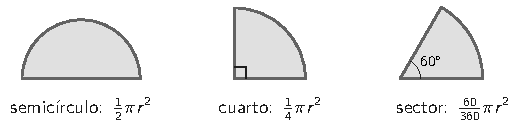
\includegraphics[width=0.5\linewidth]{geo_ci_sectores}\end{center}
\begin{ejemplo} Sector de $60°$ y radio 6: $\frac{60}{360} = \frac{1}{6}$, así que $A = \frac{1}{6} \cdot 36\pi = 6\pi$ y el arco mide $\frac{1}{6} \cdot 12\pi = 2\pi$. Semicírculo: la mitad; cuarto de círculo: la cuarta parte.\end{ejemplo}
\begin{ojo}[No olvides los lados rectos] El borde de un semicírculo es la mitad de la circunferencia \textbf{más el diámetro}: con $r = 5$, $P = 5\pi + 10$. El de un sector incluye los dos radios.\end{ojo}

\subsection{Regiones sombreadas y coronas}
\geolado[0.36]{geo_ci_sombra}{Igual que con los polígonos: área grande menos área en blanco. Un círculo que toca los cuatro lados de un cuadrado de 10 cm tiene radio 5 cm, y lo sombreado mide $100 - 25\pi \approx 21{,}5$ cm$^2$.

La \textbf{corona circular} es el anillo entre dos circunferencias de igual centro y radios $R$ y $r$: \[A = \pi R^2 - \pi r^2 = \pi(R^2 - r^2).\]}
\begin{ojo}[Corona: resta áreas, no radios] Con $R = 5$ y $r = 3$: $\pi(25 - 9) = 16\pi$. En cambio, $\pi(5 - 3)^2 = 4\pi$ está mal.\end{ojo}
\gatotip[\gatonegro]{Cuatro cuartos de círculo iguales forman un círculo completo, y dos semicircunferencias iguales, una circunferencia. ¡Junta los pedazos antes de calcular!}

\begin{elejemplo}{Tipo PAES}
\geolado[0.22]{geo_ci_ej}{En cada esquina de un cuadrado de 8 cm de lado se dibujó un cuarto de círculo con centro en el vértice y radio 4 cm, como se muestra en la figura.

¿Cuál es el área de la región sombreada?}
\alts{$(64 - 4\pi)$ cm$^2$}{$16\pi$ cm$^2$}{$(64 - 16\pi)$ cm$^2$}{$(64 - 8\pi)$ cm$^2$}
\solucion{Lo sombreado es el cuadrado menos los cuatro cuartos de círculo. El cuadrado mide $8 \cdot 8 = 64$ cm$^2$. Los cuatro cuartos, del mismo radio, forman un círculo completo de radio 4: $\pi \cdot 4^2 = 16\pi$ cm$^2$. Queda $(64 - 16\pi)$ cm$^2$.

\textit{Comprobación}: con $\pi \approx 3{,}14$, $16\pi \approx 50{,}24$ y lo sombreado mide unos 13,8 cm$^2$: positivo y menor que lo blanco \checkmark.

\textit{¿Por qué no las otras?} $(64 - 4\pi)$ resta un solo cuarto de círculo. $16\pi$ es la parte en blanco. $(64 - 8\pi)$ usa el perímetro de la circunferencia de radio 4 en vez de su área.}{C}
\end{elejemplo}
\motivacion{Los decimales de $\pi$ no se terminan nunca, y tus ganas tampoco. ¡Una vuelta completa más al temario!}

%% =====================================================================
\section{Área de superficie de cubos, paralelepípedos y cilindros}
\subsection{Los cuerpos y sus partes}
Un \textbf{paralelepípedo} (prisma recto de base rectangular) es una caja: 6 caras rectangulares, iguales de a pares. Un \textbf{cubo} tiene todas sus aristas iguales y sus 6 caras son cuadrados. Ambos tienen \textbf{6 caras, 12 aristas y 8 vértices}. Un \textbf{cilindro} tiene dos bases circulares iguales y una cara lateral curva, como una lata.
\begin{center}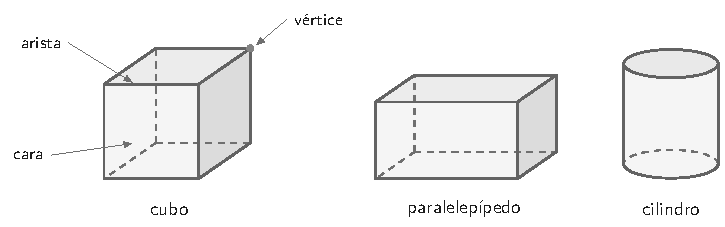
\includegraphics[width=0.62\linewidth]{geo_ac_cuerpos}\end{center}
Las líneas punteadas son aristas ocultas, que quedan detrás.

\subsection{Redes: el cuerpo desarmado}
\geolado[0.38]{geo_ac_redes}{Si desarmas una caja y la estiras sobre la mesa, obtienes su \textbf{red} o desarrollo plano. El \textbf{área de la superficie} del cuerpo es el área de su red: 6 cuadrados iguales en el cubo y 3 pares de rectángulos en el paralelepípedo.

Sirven como red de cubo la cruz y las de forma ``1--4--1''. No sirven un bloque de $2 \times 3$ ni una fila de 4 con dos cuadrados del mismo lado.}
\begin{ojo}[Truco] En una fila de 4 cuadrados, esos 4 son las paredes de alrededor; los otros dos deben ser tapa y fondo, uno a cada lado de la fila.\end{ojo}

\subsection{Área del cubo y del paralelepípedo}
\begin{clave}[Área total] Cubo de arista $a$: $6a^2$. \qquad Paralelepípedo de aristas $a$, $b$, $c$: $2(ab + bc + ac)$.\end{clave}
\begin{ejemplo} Cubo de arista 4 cm: $6 \cdot 16 = 96$ cm$^2$. Al revés, un cubo de 150 cm$^2$ tiene caras de $150 \div 6 = 25$ cm$^2$ y arista $\sqrt{25} = 5$ cm. Caja de 8, 5 y 3 cm: $2(40 + 24 + 15) = 158$ cm$^2$.\end{ejemplo}
Si el cuerpo no tiene tapa, o no se pinta la base, se resta esa cara: el cubo sin tapa tiene $5a^2$.
\begin{ojo}[No confundas con el volumen] El área total del cubo es $6a^2$ (cm$^2$); el volumen es $a^3$ (cm$^3$). Y no olvides el ``por 2'': cada tipo de cara aparece dos veces.\end{ojo}

\subsection{Área del cilindro}
\geolado[0.42]{geo_ac_red_cil}{Al abrir un cilindro, la cara lateral es un \textbf{rectángulo}: su largo es el perímetro de la base, $2\pi r$, y su ancho es la altura $h$. La etiqueta de una lata es justamente el área lateral.}
\begin{clave}[Cilindro] Lateral: $2\pi r h$ \qquad Bases: $2\pi r^2$ \qquad Total: $2\pi r h + 2\pi r^2$\end{clave}
\begin{ejemplo} Lata de radio 3 cm y altura 10 cm: lateral $60\pi$, bases $18\pi$, total $78\pi \approx 244{,}9$ cm$^2$.\end{ejemplo}
\begin{ojo}[Con diámetro] El lateral es $\pi d h$. Si pones el diámetro en lugar del radio en $2\pi r h$, el resultado sale al doble.\end{ojo}
\begin{center}\small
\begin{tabular}{lll}\toprule
Cuerpo & Área lateral & Área total\\\midrule
Cubo de arista $a$ & $4a^2$ & $6a^2$\\
Paralelepípedo $a \times b \times c$ (alto $c$) & $2(a + b)\,c$ & $2(ab + bc + ac)$\\
Cilindro de radio $r$ y altura $h$ & $2\pi r h$ & $2\pi r h + 2\pi r^2$\\\bottomrule
\end{tabular}\end{center}
\gatotip[\gatolila]{Antes de sumar, haz la lista de caras que se cuentan: ``sin tapa'', ``sin la base'', ``solo las paredes''. Y si pegas dos cuerpos, se pierden las \textbf{dos} caras que se tocan.}

\begin{elejemplo}{PAES Invierno 2026, adaptada}
\geolado[0.24]{geo_ac_mueble}{Un carpintero restaurará el siguiente mueble con forma de prisma recto de base rectangular, de 90 cm de ancho, 50 cm de fondo y 200 cm de alto.

Para la restauración, debe pintar el exterior de la estructura, sin incluir la base inferior.

¿Cuál es la medida de la superficie por pintar?}
\alts{32.500 cm$^2$}{56.000 cm$^2$}{60.500 cm$^2$}{65.000 cm$^2$}
\solucion{Calculamos el área total y le restamos la base. Frente y espalda: $2 \cdot (90 \cdot 200) = 36.000$ cm$^2$. Costados: $2 \cdot (50 \cdot 200) = 20.000$ cm$^2$. Tapa y base: $2 \cdot (90 \cdot 50) = 9000$ cm$^2$. Total: $65.000$ cm$^2$. Sin la base inferior: $65.000 - 4500 = 60.500$ cm$^2$.

\textit{Comprobación}, sumando solo lo que se pinta: $36.000 + 20.000 + 4500 = 60.500$ \checkmark.

\textit{¿Por qué no las otras?} 32.500 cm$^2$ cuenta una sola cara de cada par. 56.000 cm$^2$ quita también la tapa, que sí se pinta. 65.000 cm$^2$ incluye la base inferior.}{C}
\end{elejemplo}
\motivacion{Desarmar un cuerpo en sus caras es la clave. Ya ves las figuras por dentro y por fuera.}

%% =====================================================================
\section{Volumen de cubos, paralelepípedos y cilindros}
\subsection{¿Qué es el volumen?}
\geolado[0.28]{geo_vo_cubitos}{El \textbf{volumen} mide cuánto espacio ocupa un cuerpo: cuántos cubitos de $1 \times 1 \times 1$ caben dentro. Se mide en unidades cúbicas: cm$^3$, m$^3$.

En una caja de $4 \times 3 \times 2$ cm caben $4 \cdot 3 = 12$ cubitos en el piso y hay 2 capas: $24$ cm$^3$. Un cubo de arista $a$ tiene $V = a^3$.}
\begin{ojo}[Tres unidades distintas] Largo en cm, área en cm$^2$, volumen en cm$^3$. El volumen siempre es un producto: sumar las aristas no tiene sentido.\end{ojo}

\subsection{Paralelepípedo y cilindro}
\begin{clave}[Volumen = área de la base $\times$ altura] Cubo: $a^3$ \qquad Paralelepípedo: $a \cdot b \cdot c$ \qquad Cilindro: $\pi r^2 h$\end{clave}
\begin{ejemplo} Caja de 20, 5 y 30 cm: $3000$ cm$^3$; si se hace un 10~\% más alta, la altura pasa a 33 cm y el volumen a $3300$ cm$^3$, también un 10~\% más. Lata de radio 3 cm y altura 10 cm: $V = \pi \cdot 9 \cdot 10 = 90\pi \approx 282{,}6$ cm$^3$. Al revés: con $V = 600$, largo 10 y ancho 6, la altura es $600 \div 60 = 10$.\end{ejemplo}
\begin{ojo}[Errores del cilindro] Usar el diámetro como radio (el volumen sale 4 veces más grande), escribir $2\pi r h$ (área lateral) u olvidar elevar el radio al cuadrado. Si el cilindro está acostado, su ``altura'' es el largo.\end{ojo}

\subsection{Capacidad: litros y metros cúbicos}
La \textbf{capacidad} es el volumen que cabe dentro de un recipiente. Un cubo de 10 cm de arista contiene exactamente 1 litro.
\begin{center}\small
\begin{tabular}{ll}\toprule
Volumen & Capacidad\\\midrule
1 cm$^3$ & 1 mL\\
1 dm$^3$ $=$ 1000 cm$^3$ & 1 L\\
1 m$^3$ $=$ 1000 dm$^3$ & 1000 L\\\bottomrule
\end{tabular}\end{center}
\begin{ojo}[Tres medidas, tres veces] De m a cm se multiplica por 100, pero de m$^3$ a cm$^3$ por $100 \cdot 100 \cdot 100 = 1.000.000$. Lo más seguro es pasar las medidas a la unidad que quieras \textbf{antes} de multiplicar.\end{ojo}

\subsection{Llenado, nivel del agua y caudal}
\geolado[0.38]{geo_vo_pecera}{El agua dentro de una caja forma otra caja, con la misma base y de alto el nivel del agua.
\begin{itemize}
\item \textbf{Altura que alcanza}: 6 L $= 6000$ cm$^3$ en una pecera de base $30 \times 20$ cm suben $6000 \div 600 = 10$ cm.
\item \textbf{Objeto sumergido}: si el agua sube 2 cm, su volumen es $30 \cdot 20 \cdot 2 = 1200$ cm$^3$.
\item \textbf{Caudal}: $Q = \frac{V}{t}$. Para llenar 3000 L en 10 minutos se necesitan 300 L/min.
\end{itemize}}
\begin{ojo}[La altura del agua] Si el recipiente no está lleno, usa la altura del agua, no la del recipiente.\end{ojo}

\subsection{Cambios de escala}
\geolado[0.3]{geo_vo_escala}{Si todas las aristas se multiplican por $k$, el volumen se multiplica por $k^3$ (y el área por $k^2$): al duplicar las aristas de un cubo caben $2 \cdot 2 \cdot 2 = 8$ cubos como el original.

Si cambia una sola medida, el volumen cambia en el mismo factor. En $\pi r^2 h$ el radio cuenta doble: duplicarlo multiplica el volumen por 4; duplicar radio y altura, por 8.}
\gatotip[\gatogris]{Si un metal se funde y se rehace en piezas chicas, el volumen se conserva: divide volúmenes. Y para saber cuántas cajas caben en un contenedor, cuenta cuántas entran a lo largo de cada medida y multiplica.}

\begin{elejemplo}{PAES Invierno 2027, adaptada}
\geolado[0.26]{geo_vo_estanque}{Un estanque de agua tiene forma de prisma recto de base rectangular, cuya base mide 4 m de largo y 3 m de ancho. Se debe llenar hasta 2 m de altura con agua proveniente de un ducto.

Para calcular el caudal del agua que sale de un ducto se puede usar la expresión $\frac{V}{t}$, donde $V$ es el volumen de agua que sale del ducto durante $t$ unidades de tiempo.}
¿Cuál de las siguientes expresiones corresponde al caudal de agua, en $\frac{\text{m}^3}{\text{h}}$, que debe salir del ducto para que el estanque se llene hasta 2 m de altura en 10 horas?
\alts{$\dfrac{4 \cdot 3 \cdot 2}{10}$}{$\dfrac{4 + 3 + 2}{10}$}{$\dfrac{2(4 + 3)}{10}$}{$\dfrac{2(4 \cdot 3 + 2 \cdot 4 + 2 \cdot 3)}{10}$}
\solucion{El agua forma una caja de $4 \times 3$ m de base y 2 m de alto: $V = 4 \cdot 3 \cdot 2 = 24$ m$^3$. En $t = 10$ horas, el caudal es $\dfrac{V}{t} = \dfrac{4 \cdot 3 \cdot 2}{10}$, o sea 2,4 m$^3$ por hora.

\textit{Comprobación}: en 10 horas salen $2{,}4 \cdot 10 = 24$ m$^3$ \checkmark.

\textit{¿Por qué no las otras?} $\frac{4 + 3 + 2}{10}$ suma las medidas en vez de multiplicarlas. $\frac{2(4 + 3)}{10}$ usa el perímetro de la base por la altura, que es parte del área lateral. La última usa el área total de la caja: mide superficie, no volumen.}{A}
\end{elejemplo}
\motivacion{Llenaste otro tema hasta el borde. Tu capacidad para aprender es mucho más grande que cualquier cilindro.}

%% =====================================================================
\section{Puntos y vectores en el plano}
\subsection{El plano cartesiano y los cuadrantes}
\geolado[0.34]{tra_plano_cuadrantes}{El \textbf{plano cartesiano} tiene dos rectas numéricas perpendiculares, el \textbf{eje X} (horizontal) y el \textbf{eje Y} (vertical), que se cortan en el \textbf{origen} $O = (0, 0)$. Cada punto es un \textbf{par ordenado} $(x, y)$: primero cuánto avanzas en horizontal, después cuánto subes o bajas. $C(-2, -3)$ está 2 a la izquierda y 3 hacia abajo.

\begin{center}\small
\begin{tabular}{ccc}\toprule
Cuadrante & $x$ & $y$\\\midrule
I (arriba, derecha) & $+$ & $+$\\
II (arriba, izquierda) & $-$ & $+$\\
III (abajo, izquierda) & $-$ & $-$\\
IV (abajo, derecha) & $+$ & $-$\\\bottomrule
\end{tabular}\end{center}}

\subsection{Leer coordenadas sin equivocarse}
\textbf{El orden importa}: $(2, 5)$ y $(5, 2)$ son puntos distintos. Un punto sobre el eje X tiene $y = 0$, como $(4, 0)$; uno sobre el eje Y tiene $x = 0$, como $(0, -3)$. Los puntos de los ejes no son de ningún cuadrante.
\begin{ejemplo} Si $P(a, b)$ está en el cuadrante II, entonces $a < 0$ y $b > 0$. El punto $Q(b, a)$ tiene primera coordenada positiva y segunda negativa: está en el cuadrante IV.\end{ejemplo}
\begin{ojo}[Primero la $x$] En $(x, y)$ siempre va primero lo horizontal, como en el abecedario. Y si la cuadrícula tiene escala, multiplica los cuadros por lo que vale cada uno.\end{ojo}

\subsection{¿Qué es un vector?}
Un \textbf{vector} $\vec{u} = (a, b)$ es una flecha que indica un \textbf{desplazamiento}: $(3, 2)$ es 3 a la derecha y 2 hacia arriba. Tiene \textbf{magnitud} (su largo), \textbf{dirección} (su inclinación) y \textbf{sentido} (hacia cuál lado apunta). Flechas iguales dibujadas en distintos lugares son el mismo vector.
\begin{clave}[Vector opuesto] El opuesto de $(a, b)$ es $(-a, -b)$: misma magnitud y dirección, sentido contrario.\end{clave}

\subsection{El vector entre dos puntos: final menos inicial}
\begin{clave}[Vector de $A$ a $B$] $\overrightarrow{AB} = B - A$ (final menos inicial) \qquad Magnitud de $(a, b)$: $\sqrt{a^2 + b^2}$\end{clave}
\geolado[0.27]{tra_vector_ab}{Con $A(1, 2)$ y $B(5, -1)$: $\overrightarrow{AB} = (5 - 1, -1 - 2) = (4, -3)$: 4 a la derecha y 3 hacia abajo. Su magnitud es $\sqrt{16 + 9} = 5$.


\textit{Comprobación}: $A + (4, -3) = (5, -1) = B$ \checkmark.}
\begin{ojo}[Al revés cambia el signo] $\overrightarrow{BA} = A - B = (-4, 3)$, el opuesto de $\overrightarrow{AB}$. Y la magnitud no es la suma: $|(6, 8)| = \sqrt{100} = 10$, no 14.\end{ojo}

\subsection{Sumar vectores y multiplicarlos por un número}
\geolado[0.27]{tra_suma_vectores}{Se opera coordenada con coordenada: $(a, b) + (c, d) = (a + c, b + d)$ y $k(a, b) = (ka, kb)$.

Con $\vec{u} = (4, 1)$ y $\vec{v} = (1, 3)$: $\vec{u} + \vec{v} = (5, 4)$, $\vec{u} - \vec{v} = (3, -2)$ y $2\vec{u} = (8, 2)$. En el dibujo, la suma es hacer un desplazamiento y después el otro. Multiplicar por un número negativo da vuelta el sentido.}
\begin{ojo}[No se multiplican coordenadas] $(4, 1) + (1, 3)$ no es $(4 \cdot 1, 1 \cdot 3)$.\end{ojo}

\subsection{Trasladar un punto con un vector}
\begin{clave}[Traslación de un punto] $P' = P + \vec{v}$ \qquad y al revés \qquad $P = P' - \vec{v}$\end{clave}
\begin{ejemplo} $P(-3, 4)$ y $\vec{v} = (5, -6)$: $P' = (-3 + 5, 4 - 6) = (2, -2)$. Si $P'(1, 1)$ y $\vec{v} = (4, -2)$, entonces $P = (1 - 4, 1 - (-2)) = (-3, 3)$.\end{ejemplo}
\textbf{Dos traslaciones seguidas} equivalen a una sola con la suma de los vectores: $(2, 1)$ y luego $(3, -4)$ es lo mismo que $(5, -3)$. Con el norte hacia arriba, el este es $x$ positivo, el oeste $x$ negativo, el norte $y$ positivo y el sur $y$ negativo: ``3 km al oeste y 2 km al norte'' es $(-3, 2)$.
\gatotip[\gatonaranjo]{Comprueba siempre: el punto original más el vector debe darte la imagen. Y restar un negativo es sumar: $1 - (-2) = 3$.}
\gatotip[\gatoatigrado]{En un paralelogramo $ABCD$, el vector de $A$ a $D$ es igual al de $B$ a $C$: $D = A + (C - B)$.}

\begin{elejemplo}{PAES Invierno 2026, adaptada}
Un barco que inicia un recorrido realiza los siguientes movimientos, en este orden: 4 kilómetros al oeste, 6 kilómetros al norte, 7 kilómetros al este, 9 kilómetros al sur y 5 kilómetros al oeste.

¿Cuál es la ubicación final del barco con respecto a su ubicación inicial?
\alts{2 kilómetros al este y 3 kilómetros al norte}{16 kilómetros al oeste y 15 kilómetros al sur}{2 kilómetros al oeste y 3 kilómetros al sur}{3 kilómetros al oeste y 2 kilómetros al sur}
\solucion{Cada movimiento es un vector, con este y norte positivos: $(-4, 0)$, $(0, 6)$, $(7, 0)$, $(0, -9)$ y $(-5, 0)$. El desplazamiento total es la suma. Horizontal: $-4 + 7 - 5 = -2$, o sea 2 km al oeste. Vertical: $6 - 9 = -3$, o sea 3 km al sur. El barco termina en $(-2, -3)$: 2 km al oeste y 3 km al sur.
\begin{center}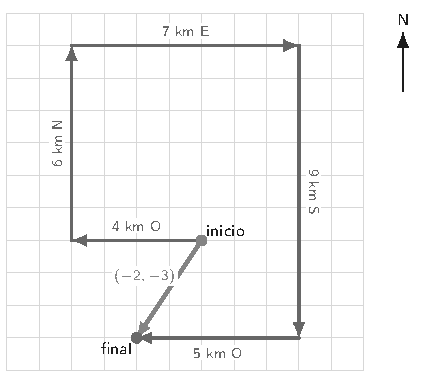
\includegraphics[width=0.3\linewidth]{tra_barco}\end{center}
\textit{Comprobación}: en la cuadrícula, la flecha que une el inicio con el final avanza 2 cuadros a la izquierda y baja 3 \checkmark.

\textit{¿Por qué no las otras?} ``2 al este y 3 al norte'' tiene los sentidos al revés. ``16 al oeste y 15 al sur'' suma todos los kilómetros sin fijarse en el sentido. ``3 al oeste y 2 al sur'' intercambia lo horizontal con lo vertical.}{C}
\end{elejemplo}
\motivacion{Ya te mueves en el plano con coordenadas y vectores. Tu vector apunta directo a la meta.}

%% =====================================================================
\section{Traslación y reflexión}
\subsection{Transformaciones isométricas}
Una \textbf{transformación isométrica} mueve una figura sin deformarla: la imagen tiene la misma forma y el mismo tamaño. Hay tres: \textbf{traslación} (desliza según un vector), \textbf{reflexión} (refleja como un espejo respecto de una recta o de un punto) y \textbf{rotación} (gira en torno a un punto). La imagen del punto $A$ se escribe $A'$.
\begin{center}\small
\begin{tabular}{lccc}\toprule
¿Se conserva? & Traslación & Reflexión & Rotación\\\midrule
Lados, ángulos, perímetro y área & sí & sí & sí\\
Orientación (sentido de recorrido de los vértices) & sí & \textbf{no}, se invierte & sí\\\bottomrule
\end{tabular}\end{center}

\subsection{Traslación de una figura}
\begin{clave}[Traslación según $(a, b)$] $(x, y) \to (x + a, y + b)$\end{clave}
\geolado[0.36]{tra_tras_triangulo}{Se traslada \textbf{cada vértice} con el mismo vector y se unen las imágenes.

Con $A(-5, 1)$, $B(-2, 1)$, $C(-4, 4)$ y $\vec{v} = (6, -3)$: $A'(1, -2)$, $B'(4, -2)$ y $C'(2, 1)$. La figura no gira ni se da vuelta. Si conoces un vértice y su imagen, el vector es imagen menos original.}

\subsection{Reflexión respecto de los ejes}
\geolado[0.3]{tra_refl_ejes}{En una reflexión, cada punto y su imagen quedan a la misma distancia del eje, uno a cada lado, en una línea perpendicular al eje.

\textbf{Respecto del eje X} la $x$ queda igual y la $y$ cambia de signo: $(x, y) \to (x, -y)$; $(3, 5) \to (3, -5)$.

\textbf{Respecto del eje Y} la $y$ queda igual y la $x$ cambia de signo: $(x, y) \to (-x, y)$; $(3, 5) \to (-3, 5)$.

La letra F de la figura queda ``al revés'', como en un espejo.}
\begin{ojo}[Para no confundirte] Cambia la coordenada que \textbf{no} lleva el nombre del eje. Reflejar respecto del eje X manda la figura hacia abajo.\end{ojo}

\subsection{\texorpdfstring{Reflexión respecto de las rectas $x = a$ e $y = b$}{Reflexión respecto de las rectas x = a e y = b}}
\geolado[0.34]{tra_refl_recta}{Cuenta la distancia del punto a la recta y pasa la misma distancia al otro lado. $B(1, 1)$ respecto de $x = 3$: de 1 a 3 hay 2 unidades; $3 + 2 = 5$ y la altura no cambia, $B' = (5, 1)$.}
\begin{clave}[Fórmulas] Respecto de $x = a$: $(x, y) \to (2a - x,\ y)$. \qquad Respecto de $y = b$: $(x, y) \to (x,\ 2b - y)$.\end{clave}
El eje queda justo \textbf{al medio} entre un punto y su imagen: el promedio de 1 y 5 es 3. Así se encuentra el eje si te dan un punto y su imagen.

\subsection{\texorpdfstring{Reflexión respecto de $y = x$ y respecto del origen}{Reflexión respecto de y = x y respecto del origen}}
\geolado[0.32]{tra_refl_yx}{\textbf{Respecto de la recta $y = x$} las coordenadas se intercambian: $(4, 1) \to (1, 4)$ y $(-2, 3) \to (3, -2)$.

\textbf{Respecto del origen} las dos coordenadas cambian de signo: $(4, 1) \to (-4, -1)$. Es lo mismo que reflejar respecto del eje X y luego del eje Y, y que girar $180^\circ$ en torno al origen.}
\begin{center}\small
\begin{tabular}{cccccc}\toprule
eje X & eje Y & recta $x = a$ & recta $y = b$ & recta $y = x$ & origen\\\midrule
$(x, -y)$ & $(-x, y)$ & $(2a - x, y)$ & $(x, 2b - y)$ & $(y, x)$ & $(-x, -y)$\\\bottomrule
\end{tabular}\end{center}
\begin{ojo}[Con $y = x$ no cambian los signos] Solo se intercambian: $(4, -1) \to (-1, 4)$.\end{ojo}

\subsection{Dos transformaciones seguidas}
Se hace la primera y a su resultado se le aplica la segunda. \textbf{El orden importa}.
\begin{ejemplo} $P(2, 3)$: reflexión respecto del eje X, $(2, -3)$, y luego traslación según $(1, 4)$, $(3, 1)$. En el otro orden da $(3, -7)$. Si la regla es $(x + 1, 4 - y)$, eso es reflejar respecto del eje X y trasladar según $(1, 4)$: la imagen de $(5, -2)$ es $(6, 6)$.\end{ejemplo}
\begin{clave}[Dos reflexiones] Respecto del mismo eje dos veces: el punto vuelve. Respecto de dos rectas paralelas: una traslación del doble de la distancia entre ellas. Respecto del eje X y luego del eje Y: la reflexión respecto del origen.\end{clave}
\gatotip[\gatoblanco]{Doblar papel es reflejar: si perforas una hoja doblada, al abrirla la perforación aparece reflejada respecto de la línea del doblez. Para deshacer dos transformaciones, deshazlas en orden inverso.}

\begin{elejemplo}{PAES Invierno 2026, adaptada}
A una figura se le aplica una reflexión y luego una traslación. La imagen del vértice $(x, y)$ es $(x - 3, 4 - y)$. A otra figura se le aplican las mismas transformaciones isométricas y en el mismo orden.

Si $(-2, -5)$ es un vértice de esta figura, ¿cuáles son las coordenadas de la imagen de este vértice?
\alts{$(-5, -1)$}{$(5, 9)$}{$(-5, 9)$}{$(-5, -9)$}
\solucion{Basta reemplazar $x = -2$ e $y = -5$ en la regla: $x - 3 = -2 - 3 = -5$ y $4 - y = 4 - (-5) = 9$. La imagen es $(-5, 9)$.

\textit{Comprobación} por pasos: la regla es una reflexión respecto del eje X seguida de una traslación según $(-3, 4)$; $(-2, -5) \to (-2, 5) \to (-5, 9)$ \checkmark.

\textit{¿Por qué no las otras?} $(-5, -1)$ calcula $4 + y$. $(5, 9)$ cambia el signo de la $x$. $(-5, -9)$ se equivoca con el menos: escribe $4 - (-5)$ como $-(4 + 5)$.}{C}
\end{elejemplo}
\motivacion{Trasladar y reflejar no cambian la figura, solo su lugar. Tú sí estás cambiando: cada tema te hace más fuerte.}

%% =====================================================================
\section{Rotación}
\subsection{¿Qué es una rotación?}
Una \textbf{rotación} gira una figura en torno a un punto fijo, el \textbf{centro de rotación}. Se describe con tres datos: el \textbf{centro} (casi siempre el origen), el \textbf{ángulo} (en la PAES, $90^\circ$, $180^\circ$ o $270^\circ$) y el \textbf{sentido}: \textbf{horario}, como los punteros del reloj, o \textbf{antihorario}, al revés. Cada punto se mantiene a la misma distancia del centro, así que la figura no cambia de tamaño ni se da vuelta.

\subsection{Las reglas de 90°, 180° y 270°}
\geolado[0.34]{tra_rot_tabla}{\begin{center}\small
\begin{tabular}{lcc}\toprule
Rotación en torno al origen & Regla & $P(4, 2)$\\\midrule
$90^\circ$ antihorario & $(-y, x)$ & $(-2, 4)$\\
$180^\circ$ (cualquier sentido) & $(-x, -y)$ & $(-4, -2)$\\
$270^\circ$ antihorario $= 90^\circ$ horario & $(y, -x)$ & $(2, -4)$\\
$360^\circ$ & $(x, y)$ & $(4, 2)$\\\bottomrule
\end{tabular}\end{center}
$270^\circ$ en un sentido es lo mismo que $90^\circ$ en el otro. $180^\circ$ da igual en un sentido o en el otro, y equivale a la reflexión respecto del centro.}
\begin{ejemplo} $90^\circ$ horario a $P(-2, 5)$: $(y, -x) = (5, 2)$. $90^\circ$ antihorario a $(4, -1)$: $(-y, x) = (1, 4)$, porque $-(-1) = 1$.\end{ejemplo}

\subsection{Trucos para no girar al revés}
\begin{clave}[Los cuadrantes] Con $90^\circ$ antihorario, cada punto avanza un cuadrante: I $\to$ II $\to$ III $\to$ IV $\to$ I. Con $90^\circ$ horario retrocede uno. Con $180^\circ$ va al cuadrante opuesto.\end{clave}
También sirve girar la hoja un cuarto de vuelta, o probar con $(1, 0)$: con $90^\circ$ antihorario debe quedar arriba, en $(0, 1)$. Varias rotaciones con el mismo centro se suman: tres de $90^\circ$ antihorario son $270^\circ$, o sea $90^\circ$ horario; cuatro devuelven la figura. Para deshacer una rotación, gira el mismo ángulo en sentido contrario.
\gatotip[\gatolila]{Los punteros del reloj giran en sentido horario, y el minutero avanza $360^\circ \div 60 = 6^\circ$ por minuto: en 20 minutos gira $120^\circ$.}

\subsection{Rotar en torno a otro punto}
\begin{clave}[Centro $C$] Mira el punto desde el centro, gíralo y vuelve: 1. resta el centro, $P - C$; 2. aplica la regla; 3. suma el centro.\end{clave}
\geolado[0.27]{tra_rot_centro}{$P(5, 2)$ en $90^\circ$ antihorario en torno a $C(2, 1)$: $P - C = (3, 1) \to (-1, 3)$, y sumando $C$, $P' = (1, 4)$.}
\begin{ojo}[No olvides volver] Quedarse con $(-1, 3)$ es el error más común: esa es la posición respecto de $C$. Con $180^\circ$, el centro es el punto medio entre el punto y su imagen: $P' = 2C - P$.\end{ojo}

\subsection{¿Qué transformación es?}
\geolado[0.28]{tra_rot_identificar}{Para reconocer qué transformación lleva una figura a otra:

\textbf{1. ¿Está dada vuelta?} Si se ve como en un espejo, es una \textbf{reflexión}.

\textbf{2. Si no, ¿está girada?} Si apunta en otra dirección, es una \textbf{rotación}; si apunta igual y solo cambió de lugar, es una \textbf{traslación}.

Después confirma aplicando la regla a un vértice. La F girada en $180^\circ$ queda cabeza abajo, pero se puede leer girando la hoja; la reflejada no.}
\gatotip[\gatonegro]{Para seguir una flecha, usa ángulos: este $0^\circ$, noreste $45^\circ$, norte $90^\circ$, sur $270^\circ$. Rotar en sentido antihorario suma grados, y una traslación nunca cambia hacia dónde apunta.}

\begin{elejemplo}{PAES Invierno 2027, adaptada}
\geolado[0.32]{tra_rot_proteina}{En el gráfico se representa una simulación bidimensional de una proteína con su grupo metilo, localizado en el punto $P(5, 3)$, con el objetivo de estudiar su desplazamiento. Dicha proteína con su grupo metilo es sometida a una rotación de $90^\circ$ en sentido antihorario con respecto al origen del sistema de coordenadas cartesianas.

¿Cuáles son las coordenadas del grupo metilo después de la rotación?}
\alts{$(3, -5)$}{$(-3, 5)$}{$(-5, -3)$}{$(5, -3)$}
\solucion{La regla de $90^\circ$ antihorario en torno al origen es $(x, y) \to (-y, x)$. Con $x = 5$ e $y = 3$ queda $(-3, 5)$.

\textit{Comprobación}: $P$ estaba en el cuadrante I y la imagen está en el II, como corresponde; además la distancia al origen se mantiene, $\sqrt{25 + 9} = \sqrt{9 + 25} = \sqrt{34}$ \checkmark.

\textit{¿Por qué no las otras?} $(3, -5)$ gira $90^\circ$ en sentido horario. $(-5, -3)$ gira $180^\circ$. $(5, -3)$ refleja respecto del eje X.}{B}
\end{elejemplo}
\motivacion{Girar en 90 o 180 grados ya no es un misterio. Y si algo sale mal, das la vuelta y lo intentas otra vez.}

%% =====================================================================
\section{Semejanza y escalas}
\subsection{Figuras semejantes}
Dos figuras son \textbf{semejantes} ($\sim$) si tienen la misma forma, aunque distinto tamaño: una es ampliación o reducción de la otra. Sus \textbf{ángulos} correspondientes son iguales y sus \textbf{lados} son \textbf{proporcionales}: todos se multiplican por el mismo número $k$, la \textbf{razón de semejanza}.
\begin{center}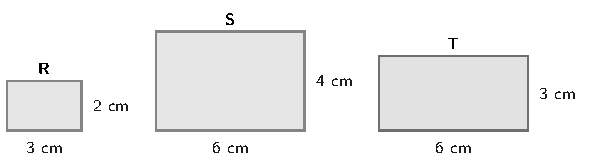
\includegraphics[width=0.52\linewidth]{sem_rectangulos}\end{center}
\begin{ejemplo} $R$ mide $3 \times 2$ y $S$ mide $6 \times 4$: $\frac{6}{3} = \frac{4}{2} = 2$, son semejantes con $k = 2$. $T$ mide $6 \times 3$: $\frac{6}{3} = 2$, pero $\frac{3}{2} = 1{,}5$; no es semejante a $R$.\end{ejemplo}
\begin{ojo}[Proporcional no es sumar lo mismo] Sumarle 3 a cada lado de $3 \times 2$ da $6 \times 5$, que no es semejante. En la semejanza se \textbf{multiplica}.\end{ojo}

\subsection{Lados homólogos y razón de semejanza}
Los \textbf{lados homólogos} son los que se corresponden. Si $\triangle ABC \sim \triangle DEF$, el orden de las letras lo dice: $AB$ con $DE$, $BC$ con $EF$ y $AC$ con $DF$.
\begin{ejemplo} $\triangle ABC \sim \triangle DEF$ con $AB = 3$, $BC = 4$, $AC = 5$, $DE = 6$ y $DF = 10$. La razón es $k = \frac{DE}{AB} = 2$ (y $\frac{DF}{AC} = 2$ lo confirma), así que $EF = 2 \cdot 4 = 8$. Con proporción: $\frac{x}{4} = \frac{6}{3}$, $3x = 24$, $x = 8$.\end{ejemplo}

\subsection{Triángulos semejantes: basta con dos ángulos}
\geolado[0.3]{sem_encajados}{Dos triángulos con \textbf{dos ángulos iguales} son semejantes (criterio AA); el tercero también es igual, porque suman $180^\circ$. También lo son si sus tres lados son proporcionales (LLL) o si dos lados son proporcionales y el ángulo entre ellos es igual (LAL).

Si en $ABC$ se traza $DE$ paralelo a $BC$, el triángulo $ADE$ es semejante a $ABC$. Con $AD = 2$, $DB = 4$ y $DE = 3$: $AB = 6$, $k = \frac{6}{2} = 3$ y $BC = 3 \cdot 3 = 9$.}
\begin{ojo}[El error clásico] El homólogo de $AB$ (lado completo del grande) es $AD$ (lado completo del chico), no el pedazo $DB$.\end{ojo}

\subsection{Sombras, postes y alturas}
\geolado[0.4]{sem_sombras}{A la misma hora, los rayos del sol llegan paralelos: cada objeto vertical, su sombra y el rayo forman triángulos rectángulos semejantes. La razón altura\,:\,sombra es la misma para todos.

Un poste de 4 m da 6 m de sombra. Una persona de 1,6 m da $\frac{1{,}6}{x} = \frac{4}{6}$, o sea $4x = 9{,}6$ y $x = 2{,}4$ m.}
\begin{ojo}[Ordena antes de calcular] Alturas arriba y sombras abajo en las dos fracciones; si mezclas, el resultado sale al revés.\end{ojo}
\gatotip[\gatogris]{Espejos en el suelo, rampas con soportes y ríos que no se pueden cruzar esconden lo mismo: dos triángulos semejantes. Empareja los lados homólogos y escribe la misma razón en ambos.}

\subsection{Planos, mapas y maquetas a escala}
Una \textbf{escala $1 : n$} significa que 1 cm del dibujo representa $n$ cm de la realidad. Del dibujo a la realidad se multiplica por $n$; de la realidad al dibujo se divide.
\begin{ejemplo} Mapa 1\,:\,50.000 con 6 cm entre dos pueblos: $6 \cdot 50.000 = 300.000$ cm $= 3000$ m $= 3$ km. Edificio de 45 m en maqueta 1\,:\,300: $\frac{4500}{300} = 15$ cm. Si 2 cm del mapa son 200 m $= 20.000$ cm, 1 cm son 10.000 cm: escala 1\,:\,10.000.\end{ejemplo}
\begin{ojo}[Mismas unidades] La escala compara centímetros con centímetros: 1 m $= 100$ cm, 1 km $= 100.000$ cm y 1 m$^2$ $= 10.000$ cm$^2$. En una escala gráfica, como ``2 cm $=$ 1 km'', cuenta cuántas veces cabe la barra.\end{ojo}

\subsection{\texorpdfstring{Perímetro por $k$, área por $k^2$}{Perímetro por k, área por k al cuadrado}}
\geolado[0.3]{sem_areas}{Si una figura se amplía con razón $k$, cada \textbf{longitud} (lados, perímetro, alturas) se multiplica por $k$ y el \textbf{área} por $k^2$: al duplicar el lado de un cuadrado caben $2 \cdot 2 = 4$ cuadrados como el original.}
\begin{ejemplo} Triángulo de perímetro 10 cm y área 4 cm$^2$, ampliado con $k = 3$: perímetro 30 cm y área $4 \cdot 9 = 36$ cm$^2$. Al revés: si las áreas de dos cuadrados son 9 y 36, $k^2 = 4$ y $k = 2$. En un plano 1\,:\,100 las áreas se multiplican por $100^2 = 10.000$.\end{ejemplo}
\gatotip[\gatoatigrado]{En un plano a escala, lo más seguro es pasar primero cada lado a la realidad y después calcular el área. Y revisa al final: lo grande debe quedar grande y lo chico, chico.}

\begin{elejemplo}{PAES Invierno 2027, adaptada}
\geolado[0.3]{sem_mapa_ruta}{Martina debe ir de su casa al colegio y para esto revisa un mapa. En la figura se presenta el mapa y la medida, en el mapa, del recorrido que debe hacer. Se sabe que 3 cm en el mapa equivalen a 150 m de distancia en la realidad.

¿Cuál es la distancia real que debe recorrer Martina?}
\alts{450 m}{650 m}{1950 m}{50 m}
\solucion{Si 3 cm son 150 m, entonces 1 cm del mapa es $\frac{150}{3} = 50$ m. El recorrido mide 13 cm en el mapa: $13 \cdot 50 = 650$ m.

\textit{Comprobación} con una proporción: $\frac{3}{150} = \frac{13}{x}$, así que $3x = 1950$ y $x = 650$ \checkmark.

\textit{¿Por qué no las otras?} 450 m multiplica 150 m por 3. 1950 m supone que cada centímetro vale 150 m. 50 m es lo que vale un solo centímetro.}{B}
\end{elejemplo}
\motivacion{Misma forma, distinto tamaño: en el mapa tus metas se ven chicas, pero a escala real son enormes. Cerraste Geometría: ¡bravo!}


\chapter{Probabilidad y Estadística}
%% Diagrama de cajón horizontal: \pyecaja{y}{mín}{Q1}{Me}{Q3}{máx}, dentro de un tikzpicture con la escala en x.
\newcommand{\pyecaja}[6]{%
  \draw[thick,gris] (#2,#1) -- (#3,#1) (#5,#1) -- (#6,#1);
  \draw[thick,gris] (#2,#1-0.18) -- (#2,#1+0.18) (#6,#1-0.18) -- (#6,#1+0.18);
  \draw[thick,nar,fill=narc!35] (#3,#1-0.32) rectangle (#5,#1+0.32);
  \draw[very thick,nard] (#4,#1-0.32) -- (#4,#1+0.32);}

%% =====================================================================
\section{Tablas de frecuencia}

\subsection{Para qué sirve una tabla}
Cuando hay muchos datos, la tabla los resume: en una columna van los valores o categorías $x_i$ y en la otra, cuántas veces aparece cada uno. Esa cantidad es la \textbf{frecuencia absoluta} $f_i$ (la PAES le dice ``cantidad'' o ``frecuencia'').

\begin{clave}[El total] $n = \sum f_i$: el total de datos se obtiene sumando la columna de frecuencias, nunca la de valores.\end{clave}

\begin{ejemplo}
Puntajes de una prueba en un curso:\par\smallskip
\centering\begin{tabular}{@{}l*{7}{c}c@{}}\toprule
Puntaje $x_i$ & 1 & 2 & 3 & 4 & 5 & 6 & 7 & Total\\\midrule
Frecuencia $f_i$ & 2 & 4 & 4 & 5 & 7 & 3 & 5 & $n = 30$\\\bottomrule
\end{tabular}\par\smallskip
\raggedright El curso tiene $2+4+4+5+7+3+5 = 30$ estudiantes; 7 es solo la cantidad de filas.
\end{ejemplo}

\subsection{Frecuencia relativa}
La \textbf{frecuencia relativa} dice qué parte del total representa cada fila. Las $h_i$ siempre suman $1$ (o $100\%$).
\begin{clave}[Relativa] \[ h_i = \frac{f_i}{n} \qquad h_i\% = \frac{f_i}{n}\cdot 100\% \qquad\text{y al revés}\qquad f_i = h_i\cdot n \]\end{clave}

\begin{minipage}[t]{0.42\linewidth}\vspace{0pt}\centering\small
\begin{tabular}{@{}ccc@{}}\toprule
Mascotas & $f_i$ & $h_i$\\\midrule
0 & 12 & $0{,}24$\\ 1 & 10 & $0{,}20$\\ 2 & 15 & $0{,}30$\\ 3 & 6 & $0{,}12$\\ 4 & 5 & $0{,}10$\\ 5 o más & 2 & $0{,}04$\\\midrule
Total & $n = 50$ & $1$\\\bottomrule
\end{tabular}
\end{minipage}\hfill
\begin{minipage}[t]{0.54\linewidth}\vspace{0pt}
\begin{ojo}[La PAES pide la expresión] Casi siempre las alternativas son del tipo $\frac{13}{50}\cdot 100\%$. Reconoce el numerador (los casos que cumplen) y el denominador ($n$): suelen poner uno bien y el otro mal.\end{ojo}
\begin{ojo}[Grupos de distinto tamaño] Para comparar niveles con distinta cantidad de alumnos se comparan porcentajes, cada uno sobre su propio total: $\frac{20}{80} = 25\%$ es mayor que $\frac{25}{125} = 20\%$, aunque 25 sea más que 20.\end{ojo}
\end{minipage}

\subsection{Frecuencias acumuladas}
La \textbf{acumulada} $F_i = f_1 + \dots + f_i$ suma desde la primera fila hasta la fila $i$, y $H_i = F_i/n$ es la relativa acumulada. Como crece fila a fila, $f_i = F_i - F_{i-1}$: si $F_3 = 20$ y $F_2 = 14$, entonces $f_3 = 6$.

\begin{clave}[Traducción]
``A lo más 2'' o ``no supera 2'' $=$ 2 o menos: se acumula hasta la fila del 2.\\
``Al menos 3'' o ``como mínimo 3'' $=$ 3 o más: se suman las filas desde el 3, o bien $n - F_2$.\\
``Más de 3'' $=$ 4 o más (el 3 no entra). ``Menos de 3'' $=$ 0, 1 o 2.
\end{clave}

\begin{ejemplo} Con la tabla de mascotas: familias con 3 o más son $6+5+2 = 13$, es decir $\frac{13}{50}\cdot 100\% = 26\%$. Con a lo más 2 son $12+10+15 = 37 = F_3$ y $H_3 = 0{,}74$.\end{ejemplo}

\subsection{Categorías abiertas e intervalos}
Filas como ``5 o más'' o ``18--24 años'' dicen cuántos datos hay, pero no su valor exacto. Cuando el límite pedido cae \textbf{dentro} de un intervalo, la respuesta depende de si piden la mayor o la menor cantidad posible.

\begin{ojo}[Máximo y mínimo] ¿Cuántos trabajadores, como máximo, tienen a lo más 40 años? La fila 35--44 contiene el 40: para el \textbf{máximo} cuenta entera; para el \textbf{mínimo} aporta 0.\end{ojo}

\gatotip[\gatonaranjo]{Antes de sumar, marca con el lápiz las filas que cumplen la condición. ``Como mínimo 6'' incluye al 6: es el descuido que más puntos regala.}

\begin{elejemplo}{PAES Invierno 2027, adaptada}
En la siguiente tabla se presenta el tiempo que las personas han trabajado en un colegio.
\begin{center}\small
\begin{tabular}{@{}l*{10}{c}@{}}\toprule
Tiempo de trabajo en años & 1 & 2 & 3 & 4 & 5 & 6 & 7 & 8 & 9 & 10\\\midrule
Cantidad de personas & 2 & 4 & 5 & 4 & 2 & 6 & 2 & 5 & 3 & 2\\\bottomrule
\end{tabular}
\end{center}
El colegio entregará un bono a quienes hayan trabajado \textbf{como mínimo 6 años}. ¿Cuántas personas recibirán el bono?
\alts{12}{17}{18}{23}
\solucion{``Como mínimo 6 años'' significa 6 o más: se suman las filas 6, 7, 8, 9 y 10, es decir $6+2+5+3+2 = 18$ personas. Los distractores: 12 es sumar desde 7 (dejar fuera el 6); 17 es sumar de 1 a 5 (los que \textbf{no} reciben bono); 23 es sumar desde 5.}{C}
\end{elejemplo}

%% =====================================================================
\section{Gráficos}

\subsection{Cada gráfico cuenta algo distinto}
El gráfico de \textbf{barras} compara categorías: la altura es $f_i$ o $h_i\%$. El \textbf{circular} muestra partes de un total. El de \textbf{líneas} muestra cómo cambia algo en el tiempo. En un \textbf{pictograma} cada ícono vale una cantidad fija: 16 íconos de 4 personas son 64 personas.

\begin{clave}[Para elegir gráfico] ¿Categorías que se comparan? Barras. ¿Porcentajes que suman $100\%$? Circular. ¿Algo que cambia en el tiempo? Líneas.\end{clave}
\begin{ojo}[Mira el eje] Si el eje está en $\%$, la altura no es la cantidad: el $25\%$ de 80 alumnos son $0{,}25\cdot 80 = 20$.\end{ojo}

\begin{minipage}[c]{0.46\linewidth}\centering
\begin{tikzpicture}
\begin{axis}[ybar,width=6.4cm,height=4.4cm,ymin=0,ymax=8.5,bar width=13pt,xtick={1,...,5},xticklabels={Lun,Mar,Mié,Jue,Vie},
  axis lines*=left,ylabel={celulares},nodes near coords,every node near coord/.append style={font=\scriptsize},tick label style={font=\small},enlarge x limits=0.15,ytick={0,2,...,8}]
\addplot[fill=nar,draw=nard] coordinates {(1,3) (2,6) (3,5) (4,2) (5,7)};
\draw[dashed,azul,thick] (axis cs:0.4,5) -- (axis cs:5.6,5);
\end{axis}
\end{tikzpicture}
\end{minipage}\hfill
\begin{minipage}[c]{0.5\linewidth}
Celulares vendidos por día. Si la meta es vender \textbf{al menos 5}, se cumple el martes, el miércoles y el viernes: el 5 cuenta.
\end{minipage}

\subsection{Gráfico circular}
Cada sector es una frecuencia relativa y el círculo completo es el $100\%$. Un sector de $90^\circ$ es $\frac{90}{360} = \frac14 = 25\%$ del total.
\begin{clave}[Circular] \[ \text{ángulo}_i = h_i\cdot 360^\circ \qquad f_i = h_i\cdot n \qquad n = \frac{f_i}{h_i} \]\end{clave}
\begin{ejemplo} De 240 encuestados, el sector de $90^\circ$ son $0{,}25\cdot 240 = 60$ personas. Y al revés: si 85 artículos son el $25\%$, el total es $\frac{85}{0{,}25} = 340$.\end{ejemplo}

\subsection{Gráfico de líneas}
Interesan la tendencia, los máximos y mínimos, y las subidas y bajadas. ``Aumentó mes a mes'' exige que cada punto esté más arriba que el anterior: basta una bajada para que sea falso.

\begin{minipage}[t]{0.5\linewidth}\vspace{0pt}
\begin{clave}[Mayor aumento] Es la mayor diferencia entre dos puntos \textbf{consecutivos}, no el punto más alto. Aquí: $+2$, $+3$, $-1$, $+6$, $-2$; el mayor aumento es entre abril y mayo.\end{clave}
\begin{ojo}[Ausencia no es cero] Si un mes no aparece en el gráfico, el gráfico no informa nada de ese mes.\end{ojo}
\end{minipage}\hfill
\begin{minipage}[t]{0.46\linewidth}\vspace{0pt}\centering
\begin{tikzpicture}
\begin{axis}[width=6.4cm,height=4.4cm,ymin=8,ymax=22,xtick={1,...,6},xticklabels={Ene,Feb,Mar,Abr,May,Jun},axis lines*=left,
  ylabel={miles de unidades},tick label style={font=\small},label style={font=\small},enlarge x limits=0.08]
\addplot[nar,very thick,mark=*,mark options={fill=white}] coordinates {(1,10) (2,12) (3,15) (4,14) (5,20) (6,18)};
\end{axis}
\end{tikzpicture}
\end{minipage}

\subsection{Gráficos engañosos}
La PAES pregunta por qué un gráfico dificulta una comparación. Las causas típicas son dos gráficos con \textbf{escalas distintas} (una barra de $20\%$ puede verse más alta que una de $30\%$), un eje vertical que \textbf{no parte de 0} (exagera las diferencias) y sectores 3D o barras de ancho distinto (distorsionan el área).

\gatotip[\gatogris]{Antes de comparar dos gráficos a ojo, mira que compartan escala y unidad. Si no, olvida las alturas y compara los números.}
\gatotip[\gatoatigrado]{``Más frecuente'' es la barra más alta, la moda. Si cada hora extra se paga \peso 15.000 y la barra más alta es la de 3 horas, el pago más frecuente es \peso 45.000.}

\begin{elejemplo}{PAES Invierno 2026, adaptada}
Los artículos de una tienda de jardinería están clasificados en cinco categorías. La cantidad de artículos vendidos en cierta semana se presenta en el siguiente gráfico circular.
\begin{center}
\begin{tikzpicture}[font=\small]
\def\r{1.45}
\fill[nar] (0,0) -- (90:\r) arc[start angle=90,end angle=198,radius=\r] -- cycle;
\fill[azul] (0,0) -- (198:\r) arc[start angle=198,end angle=270,radius=\r] -- cycle;
\fill[menta] (0,0) -- (270:\r) arc[start angle=270,end angle=360,radius=\r] -- cycle;
\fill[lila] (0,0) -- (0:\r) arc[start angle=0,end angle=54,radius=\r] -- cycle;
\fill[narc] (0,0) -- (54:\r) arc[start angle=54,end angle=90,radius=\r] -- cycle;
\foreach \a in {90,198,270,0,54} \draw[white,thick] (0,0) -- (\a:\r);
\node at (144:2.35) {Flores $30\%$};
\node at (234:2.35) {Árboles $20\%$};
\node at (315:2.4) {Semillas $25\%$};
\node at (27:2.35) {Tierra $15\%$};
\node at (72:2.0) {Arbustos $10\%$};
\end{tikzpicture}
\end{center}
Si esa semana se vendieron 85 semillas, ¿cuál fue el total de artículos vendidos?
\alts{200}{300}{340}{500}
\solucion{Semillas es el $25\%$ del total y corresponde a 85 artículos: $0{,}25\cdot n = 85$, así que $n = \frac{85}{0{,}25} = 85\cdot 4 = 340$. Comprobación: el $30\%$ de 340 son 102 flores, el $20\%$ son 68 árboles, etc.; todo suma 340.}{C}
\end{elejemplo}

%% =====================================================================
\section{Promedio}

\subsection{El promedio reparte el total en partes iguales}
\begin{clave}[Promedio] \[ \bar{x} = \frac{x_1 + x_2 + \dots + x_n}{n} = \frac{\sum x_i}{n} \qquad\text{y al revés}\qquad \sum x_i = n\cdot\bar{x} \]\end{clave}
\begin{ejemplo} Gasto en almuerzo durante una semana: \peso 3.200, \peso 5.300, \peso 7.200, \peso 2.500, \peso 11.400, \peso 12.000 y \peso 6.000. La suma es \peso 47.600 y $\bar{x} = \frac{47.600}{7} = 6.800$ pesos diarios. Se divide por 7, incluido el fin de semana.\end{ejemplo}
El promedio no tiene por qué ser uno de los datos, y un valor extremo lo arrastra. Si la pregunta selecciona algunos datos (por ejemplo, de junio a septiembre), se promedian solo esos.

\subsection{Promedio desde una tabla de frecuencias}
Cada valor $x_i$ aparece $f_i$ veces, así que se multiplica antes de sumar.

\begin{minipage}[t]{0.55\linewidth}\vspace{0pt}
\begin{clave}[Promedio de una tabla] \[ \bar{x} = \frac{\sum f_i\,x_i}{n} = \sum h_i\,x_i \]
Con valores 0, 1 y 2 y frecuencias $P$, $Q$ y $R$:
\[ \bar{x} = \frac{0\cdot P + 1\cdot Q + 2\cdot R}{P + Q + R} \]\end{clave}
\begin{ojo}[Denominador] Se divide por la suma de \textbf{todas} las frecuencias, no por la cantidad de filas.\end{ojo}
\end{minipage}\hfill
\begin{minipage}[t]{0.4\linewidth}\vspace{0pt}\centering\small
\begin{tabular}{@{}ccc@{}}\toprule
Mascotas $x_i$ & $f_i$ & $f_i\,x_i$\\\midrule
0 & 12 & 0\\ 1 & 10 & 10\\ 2 & 15 & 30\\ 3 & 6 & 18\\ 4 & 5 & 20\\\midrule
Total & 48 & 78\\\bottomrule
\end{tabular}\par\smallskip
$\bar{x} = \dfrac{78}{48} = 1{,}625$ mascotas por familia.
\end{minipage}

\subsection{Cómo cambia el promedio}
Si a \textbf{todos} los datos se les suma $k$, el promedio aumenta en $k$; si se multiplican por $k$, el promedio se multiplica por $k$. Si se \textbf{agrega} un dato mayor que $\bar{x}$, el promedio sube; si es menor, baja; si es igual, no cambia. Si se \textbf{quita} un dato mayor que $\bar{x}$, el promedio baja; si se quita uno menor, sube.

\begin{clave}[Promedio de grupos] \[ \bar{x} = \frac{n_A\,\bar{x}_A + n_B\,\bar{x}_B}{n_A + n_B} \]
Los promedios se pueden promediar directamente solo si los grupos tienen el \textbf{mismo tamaño}.\end{clave}

\subsection{Despejar un dato desconocido}
Para saber qué nota falta: el total necesario es $n\cdot\bar{x}$, se le resta lo que ya se tiene y lo que queda es el dato.
\begin{ejemplo} Notas 5,0; 6,0 y 4,5, y se quiere promedio 5,5 con cuatro notas: $4\cdot 5{,}5 = 22$ y $22 - 15{,}5 = 6{,}5$.\end{ejemplo}
\begin{ojo}[Crecimiento promedio] Un brote midió 2 cm y cinco semanas después 14 cm: creció $14 - 2 = 12$ cm, o sea $\frac{12}{5} = 2{,}4$ cm por semana. Se promedia el \textbf{cambio}, no la altura final.\end{ojo}

\gatotip[\gatoblanco]{Si las alternativas traen $P$, $Q$ y $R$, revisa dos cosas: arriba cada valor multiplicado por su frecuencia, abajo la suma de todas las frecuencias.}

\begin{elejemplo}{PAES Invierno 2027, adaptada}
El promedio de edad de un grupo A de personas es 30 años, mientras que el promedio de edad de un grupo B es 40 años. Si se quiere cambiar solo a una persona de grupo, ¿en cuál de los siguientes casos el promedio \textbf{aumentará en ambos grupos}?
\alts{Que se cambie una persona de 45 años del grupo B al grupo A.}{Que se cambie una persona de 35 años del grupo B al grupo A.}{Que se cambie una persona de 45 años del grupo A al grupo B.}{Que se cambie una persona de 30 años del grupo A al grupo B.}
\solucion{Para que el grupo que \textbf{pierde} a la persona suba su promedio, la persona debe ser menor que ese promedio. Para que el grupo que la \textbf{recibe} suba, debe ser mayor que su promedio. Una persona de 35 años sale de B ($35 < 40$): B sube; entra a A ($35 > 30$): A sube. En cambio, 45 de B a A hace bajar a B; 45 de A a B hace bajar a A; y 30 de A a B deja igual a A y hace bajar a B.}{B}
\end{elejemplo}

%% =====================================================================
\section{Cuartiles y percentiles}

\subsection{Primero, ordenar}
Las medidas de posición dividen los datos \textbf{ordenados de menor a mayor} en partes con la misma cantidad de datos. La \textbf{mediana} $Me = Q_2$ deja la mitad de los datos a cada lado.
\begin{clave}[Mediana] Si $n$ es impar, es el dato del centro. Si $n$ es par, es el promedio de los dos centrales.\end{clave}
\begin{ejemplo} 3, 5, 7, 8, 10, 12 ($n = 6$): $Me = \frac{7+8}{2} = 7{,}5$. Y 4, 0, 0, 2, 3, 3, 1, 0, 3 ordenados quedan 0, 0, 0, 1, \textbf{2}, 3, 3, 3, 4: $Me = 2$.\end{ejemplo}

\subsection{Cuartiles: cuatro partes iguales}
$Q_1$ es la mediana de la \textbf{mitad inferior} (los datos antes de $Me$) y $Q_3$ es la mediana de la \textbf{mitad superior}. Si $n$ es impar, la mediana no se incluye en ninguna mitad. El \textbf{rango intercuartil} $RIC = Q_3 - Q_1$ es el ancho del $50\%$ central.
\begin{ejemplo} En 0, 0, 0, 1, \textbf{2}, 3, 3, 3, 4: la mitad inferior 0, 0, 0, 1 da $Q_1 = 0$; la superior 3, 3, 3, 4 da $Q_3 = 3$; $RIC = 3$.\\
En 2, 4, 4, 6, 9, 10, 12, 15 ($n = 8$): $Q_3 = \frac{10+12}{2} = 11$, que no es ninguno de los datos.\end{ejemplo}
\begin{ojo}[Error frecuente] $Q_1$ no es el punto medio entre el mínimo y la mediana: es la mediana de los \textbf{datos} de la mitad inferior.\end{ojo}

\subsection{Percentiles: cien partes}
El percentil $P_k$ es el valor que deja \textbf{al menos el $k\%$} de los datos en $P_k$ o por debajo. Así, $P_{25} = Q_1$, $P_{50} = Me$ y $P_{75} = Q_3$.
\begin{clave}[Interpretar] ``$P_{80} = 65$ puntos'': al menos el $80\%$ obtuvo 65 puntos o menos (y a lo más el $20\%$ obtuvo más). El valor (65) y el porcentaje (80) no son intercambiables.\end{clave}
\begin{ejemplo} En un grupo de 40, quien supera a 30 está sobre el $\frac{30}{40} = 75\%$: su puntaje está en el percentil 75.\end{ejemplo}

\subsection{Cuartiles desde una tabla de frecuencias}
Se calcula la acumulada $F_i$ y se busca la posición que interesa ($\frac{n}{4}$, $\frac{n}{2}$ o $\frac{3n}{4}$): el valor es el de la primera fila donde $F_i$ la alcanza.

\begin{minipage}[t]{0.36\linewidth}\vspace{0pt}\centering\small
\begin{tabular}{@{}ccc@{}}\toprule
Puntaje & $f_i$ & $F_i$\\\midrule
1 & 2 & 2\\ 2 & 4 & 6\\ 3 & 4 & 10\\ 4 & 5 & 15\\ 5 & 7 & 22\\ 6 & 3 & 25\\ 7 & 5 & 30\\\bottomrule
\end{tabular}
\end{minipage}\hfill
\begin{minipage}[t]{0.6\linewidth}\vspace{0pt}
\begin{ejemplo} Con $n = 30$ la mediana promedia las posiciones 15 y 16. La primera fila con $F_i \ge 15$ es el puntaje 4; la primera con $F_i \ge 16$ es el 5. Entonces $Me = \frac{4+5}{2} = 4{,}5$.\end{ejemplo}
\gatotip[\gatolila]{Al terminar, revisa que $Q_1 \le Me \le Q_3$. Si no se cumple, algo quedó mal ordenado.}
\end{minipage}

\begin{elejemplo}{PAES Invierno 2027, adaptada}
Para una tarea, una estudiante debe representar con un diagrama de cajón las anotaciones positivas de sus amigos: 4, 0, 0, 2, 3, 3, 1, 0, 3. Realiza los siguientes pasos, cometiendo un error:\par\smallskip
\textbf{Paso 1:} ordena los datos de menor a mayor y determina que el dato central es 2.\\
\textbf{Paso 2:} identifica el mínimo y el máximo, obteniendo 0 y 4.\\
\textbf{Paso 3:} determina el primer cuartil como 1, ya que se encuentra entre 0 y 2, y el tercer cuartil como 3, ya que se encuentra entre 2 y 4.\\
\textbf{Paso 4:} construye el diagrama con esos cinco valores.\par\smallskip
¿En cuál de los pasos cometió el error?
\alts{En el Paso 1}{En el Paso 2}{En el Paso 3}{En el Paso 4}
\solucion{Ordenados: 0, 0, 0, 1, \textbf{2}, 3, 3, 3, 4. El Paso 1 es correcto ($Me = 2$) y el Paso 2 también (mínimo 0, máximo 4). En el Paso 3, $Q_1$ es la mediana de la mitad inferior 0, 0, 0, 1, o sea $0$, no ``el número que está entre 0 y 2''. $Q_3$ es la mediana de 3, 3, 3, 4, que es 3: le resultó bien por casualidad. El error está en el Paso 3: los cuartiles no son puntos medios entre el mínimo y la mediana, sino medianas de las mitades de los datos.}{C}
\end{elejemplo}

%% =====================================================================
\section{Diagrama de cajón}

\subsection{Cinco números, un dibujo}
El diagrama de cajón resume los datos con cinco números: \textbf{mínimo, $Q_1$, $Me$, $Q_3$ y máximo}. La caja va de $Q_1$ a $Q_3$ y contiene el $50\%$ central; la línea dentro de la caja es la mediana; los bigotes llegan al mínimo y al máximo. El ancho de la caja es el $RIC$.

\begin{center}
\begin{tikzpicture}[x=0.17cm,font=\small]
\draw[gris] (0,-0.7) -- (40,-0.7);
\foreach \t in {0,10,20,30,40} \draw[gris] (\t,-0.6) -- (\t,-0.8) node[below] {\t};
\pyecaja{0}{4}{12}{18}{26}{36}
\foreach \v/\lab in {4/mín,12/$Q_1$,18/$Me$,26/$Q_3$,36/máx} \node[above,font=\scriptsize] at (\v,0.38) {\lab};
\end{tikzpicture}
\end{center}
\begin{clave}[Cada tramo, al menos un $25\%$] mín a $Q_1$, $Q_1$ a $Me$, $Me$ a $Q_3$ y $Q_3$ a máx reúnen cada uno al menos el $25\%$ de los datos. Hasta $Q_3$ hay al menos un $75\%$; desde $Q_3$ hacia arriba, al menos un $25\%$.\end{clave}

\subsection{Lo que el cajón dice y lo que no}
Sí se puede afirmar que al menos el $25\%$ de los datos es menor o igual que $Q_1$, al menos el $50\%$ es menor o igual que $Me$ y al menos el $75\%$ es menor o igual que $Q_3$, y que ningún dato queda fuera de los bigotes.
\begin{ojo}[No se puede afirmar] El \textbf{promedio} (el cajón no lo muestra), \textbf{cuántos} datos hay, ni que ``la mitad tiene exactamente $Me$''. Un valor del cajón tampoco es un porcentaje ni una posición en el orden.\end{ojo}
\begin{ejemplo} Seguidores: mín 80, $Q_1 = 140$, $Me = 270$, $Q_3 = 400$, máx 600. Es correcto decir que al menos un $25\%$ tiene entre 140 y 270 seguidores; no lo es decir que el promedio es 270.\end{ejemplo}

\subsection{Construir el cajón desde los datos}
Con 18, 19, 20, 21, 21, 27, 30, 30, 31, 34, 35 ($n = 11$): mínimo 18 y máximo 35; $Me = 27$ (posición 6); $Q_1$ es la mediana de 18, 19, 20, 21, 21, o sea 20; $Q_3$ es la mediana de 30, 30, 31, 34, 35, o sea 31.
\begin{center}
\begin{tikzpicture}[x=0.26cm,font=\small]
\draw[gris] (15,-0.7) -- (40,-0.7);
\foreach \t in {15,20,...,40} \draw[gris] (\t,-0.6) -- (\t,-0.8) node[below] {\t};
\pyecaja{0}{18}{20}{27}{31}{35}
\foreach \v in {20,27,31,35} \node[above,font=\scriptsize] at (\v,0.38) {\v};
\node[above left,font=\scriptsize,inner xsep=1pt] at (18,0.38) {18};
\end{tikzpicture}
\end{center}
\gatotip[\gatonegro]{Para elegir entre cuatro cajones, compara primero los extremos, después la mediana y al final los cuartiles. Descartas rápido.}

\subsection{Comparar grupos}
Una mediana más a la derecha indica valores mayores en general. Una caja más ancha (mayor $RIC$) indica que el $50\%$ central está más \textbf{disperso}; la mediana no mide dispersión. Un bigote largo hacia un lado indica datos estirados hacia ese lado.

\begin{minipage}[c]{0.5\linewidth}\centering
\begin{tikzpicture}[x=0.11cm,y=0.9cm,font=\small]
\draw[gris] (0,-0.7) -- (60,-0.7);
\foreach \t in {0,10,...,60} \draw[gris] (\t,-0.6) -- (\t,-0.8) node[below] {\t};
\pyecaja{0.9}{10}{18}{24}{30}{42}
\pyecaja{0}{14}{26}{36}{48}{58}
\node[left] at (8,0.9) {A}; \node[left] at (12,0) {B};
\end{tikzpicture}
\end{minipage}\hfill
\begin{minipage}[c]{0.46\linewidth}
B tiene mayor mediana (36 contra 24) y mayor $RIC$ ($48 - 26 = 22$ contra $30 - 18 = 12$): valores más altos, pero más dispersos. Como el mínimo de B es menor que el máximo de A, no se puede decir que todos los de B superan a todos los de A.
\end{minipage}

\begin{elejemplo}{PAES Invierno 2027, adaptada}
En el siguiente diagrama de cajón se presenta el tiempo, en minutos, que tardó un grupo de personas en completar un circuito deportivo.
\begin{center}
\begin{tikzpicture}[x=0.36cm,font=\small]
\draw[gris] (6,-0.7) -- (24,-0.7);
\foreach \t in {6,9,...,24} \draw[gris] (\t,-0.6) -- (\t,-0.8) node[below] {\t};
\pyecaja{0}{8}{12}{14}{16}{22}
\foreach \v in {8,12,14,16,22} \node[above,font=\scriptsize] at (\v,0.38) {\v};
\end{tikzpicture}
\end{center}
¿Qué representa el 16 en el diagrama de cajón?
\alts{Que al menos un $75\%$ de las personas terminó el circuito en 16 minutos o menos.}{Que un $16\%$ de las personas terminó el circuito en a lo más 16 minutos.}{Que la dieciseisava persona que terminó el circuito demoró 16 minutos.}{Que la cuarta persona que terminó el circuito demoró 16 minutos.}
\solucion{El 16 es el borde derecho de la caja: es $Q_3$, el tercer cuartil, que deja al menos el $75\%$ de los datos en 16 o menos. Eso es exactamente la alternativa A. Las otras confunden el valor 16 con un porcentaje o con una posición en el orden de llegada, cosas que el cajón no informa.}{A}
\end{elejemplo}

%% =====================================================================
\section{Probabilidad de un evento}

\subsection{Experimento, espacio muestral y evento}
Un \textbf{experimento aleatorio} es uno en que se conocen los resultados posibles, pero no cuál saldrá, como lanzar un dado. El \textbf{espacio muestral} $\Omega$ reúne todos los resultados posibles: para un dado común, $\Omega = \{1,2,3,4,5,6\}$ y $\#\Omega = 6$. Un \textbf{evento} es un subconjunto de $\Omega$; ``sale par'' es $A = \{2,4,6\}$.
\begin{clave}[Regla de Laplace] Si todos los resultados son igualmente probables,
\[ \mathbb{P}(A) = \frac{\#\,\text{casos favorables}}{\#\,\text{casos totales}} = \frac{\#A}{\#\Omega}, \qquad 0 \le \mathbb{P}(A) \le 1. \]
Así, $\mathbb{P}(\text{par}) = \frac36 = \frac12$. Una probabilidad 0 es imposible y 1 es seguro.\end{clave}

\subsection{Contar bien los casos}
Con \textbf{dos dados} hay $6\cdot 6 = 36$ pares ordenados. La suma 7 sale con (1,6), (2,5), (3,4), (4,3), (5,2) y (6,1): es la suma más probable, con $\frac{6}{36}$; la suma 6 sale de 5 maneras, la 10 de 3 y la 12 de una sola. Con \textbf{tres monedas} hay $2^3 = 8$ resultados: CCC, CCS, CSC, SCC, CSS, SCS, SSC, SSS.
\begin{ojo}[Lo que ya salió cambia $\Omega$] En un memorice de 20 tarjetas ya volteaste un rayo: quedan 19 tarjetas y solo una es el otro rayo, así que $\mathbb{P} = \frac{1}{19}$, no $\frac{1}{20}$.\end{ojo}
Si el enunciado da frecuencias (en una tabla o en un gráfico), los casos totales son $n$, la suma de todas las barras, y los favorables son la frecuencia de la categoría: si 9 de 28 personas prefieren computador, $\mathbb{P} = \frac{9}{28}$. Si piden una categoría \textbf{o} otra distinta, se suman sus frecuencias sobre el mismo total: $\frac{64 + 51}{441}$.

\subsection{Tablas de doble entrada}
\begin{minipage}[t]{0.38\linewidth}\vspace{0pt}\centering\small
\begin{tabular}{@{}lcc@{}}\toprule
Área & Hombre & Mujer\\\midrule
Científica & 7 & 10\\ Humanista & 4 & 6\\ Matemática & 8 & 9\\ Artística & 3 & 5\\\midrule
Total & 22 & 30\\\bottomrule
\end{tabular}
\end{minipage}\hfill
\begin{minipage}[t]{0.58\linewidth}\vspace{0pt}
Con $n = 52$: ``mujer \textbf{y} artística'' es una sola celda, $\frac{5}{52}$; ``mujer'' es una columna completa, $\frac{30}{52}$; ``artística'' es una fila completa, $\frac{8}{52}$.
\end{minipage}
\begin{clave}[El denominador] Es el total de la tabla, salvo que la pregunta restrinja el grupo: ``si se elige una mujer al azar\dots'' cambia el denominador a 30.\end{clave}

\subsection{Cuando los resultados no son equiprobables}
Un \textbf{dado cargado} viene con su tabla de probabilidades, que suman 1. Ya no se cuentan casos: se \textbf{suman las probabilidades} de los resultados favorables.
\begin{center}\small
\begin{tabular}{@{}l*{6}{c}@{}}\toprule
Cara & 1 & 2 & 3 & 4 & 5 & 6\\\midrule
$\mathbb{P}$ & $0{,}2$ & $0{,}1$ & $0{,}1$ & $0{,}1$ & $0{,}4$ & $0{,}1$\\\bottomrule
\end{tabular}
\end{center}
\begin{ejemplo} $\mathbb{P}(\text{mayor que } 4) = 0{,}4 + 0{,}1 = 0{,}5$ y $\mathbb{P}(\text{par}) = 0{,}1 + 0{,}1 + 0{,}1 = 0{,}3$. Comparado con un dado común, $\mathbb{P}(6) = 0{,}1 < \frac16$.\end{ejemplo}
\begin{clave}[Complemento] $\mathbb{P}(A^c) = 1 - \mathbb{P}(A)$. Si $\mathbb{P}(\text{lluvia}) = 0{,}3$, entonces $\mathbb{P}(\text{no lluvia}) = 0{,}7$; en una ruleta de 9 partes con 2 fantasmas, $\mathbb{P}(\text{no fantasma}) = 1 - \frac29 = \frac79$.\end{clave}

\gatotip[\gatoatigrado]{Escribe primero el denominador: ¿cuántos casos hay \textbf{ahora}? Después cuenta los favorables. La mayoría de los distractores tienen el denominador equivocado.}

\begin{elejemplo}{PAES Invierno 2026, adaptada}
En la tabla se presentan los resultados de una encuesta a un grupo de estudiantes sobre el área de preferencia para sus estudios superiores.
\begin{center}\small
\begin{tabular}{@{}lcc@{}}\toprule
Área de preferencia & Hombre & Mujer\\\midrule
Científica & 7 & 10\\ Humanista & 4 & 6\\ Matemática & 8 & 9\\ Artística & 3 & 5\\\bottomrule
\end{tabular}
\end{center}
Si se selecciona al azar a una persona del grupo, ¿cuál es la probabilidad de que sea mujer y que escoja el área artística?
\alts{$\frac{5}{52}$}{$\frac{1}{5}$}{$\frac{5}{8}$}{$\frac{5}{30}$}
\solucion{Casos totales: toda la tabla, $n = 7+10+4+6+8+9+3+5 = 52$. Casos favorables: la celda ``mujer y artística'', que es 5. Entonces $\mathbb{P} = \frac{5}{52}$. La alternativa $\frac58$ restringe a los del área artística y $\frac{5}{30}$ restringe a las mujeres; ninguna restricción aparece en el enunciado.}{A}
\end{elejemplo}

%% =====================================================================
\section{Regla aditiva y multiplicativa}

\subsection{Regla aditiva: ``A o B''}
Si $A$ y $B$ \textbf{no pueden ocurrir juntos} (son mutuamente excluyentes, $A\cap B = \emptyset$), sus probabilidades se suman. Si pueden ocurrir juntos, lo común quedó contado dos veces y se descuenta.
\begin{clave}[Regla aditiva] \[ \mathbb{P}(A\cup B) = \mathbb{P}(A) + \mathbb{P}(B) - \mathbb{P}(A\cap B) \]
Para eventos excluyentes, $\mathbb{P}(A\cap B) = 0$ y queda $\mathbb{P}(A) + \mathbb{P}(B)$.\end{clave}
\begin{ejemplo} ``Sale 1 o 2'': $\frac16 + \frac16 = \frac13$. ``Par o mayor que 4'': pares $\{2,4,6\}$, mayores que 4 $\{5,6\}$, en común $\{6\}$; $\frac36 + \frac26 - \frac16 = \frac46$. Comprobación: $\{2,4,5,6\}$ son 4 casos.\end{ejemplo}

\subsection{Regla multiplicativa: ``A y luego B''}
Si los experimentos son \textbf{independientes} (uno no cambia al otro), las probabilidades se multiplican: $\mathbb{P}(A\cap B) = \mathbb{P}(A)\cdot\mathbb{P}(B)$. Un dado y una moneda, ``par y cara'': $\frac12\cdot\frac12 = \frac14$. Dos seis seguidos: $\frac16\cdot\frac16 = \frac{1}{36}$.

\begin{minipage}[t]{0.48\linewidth}\vspace{0pt}
\begin{clave}[Con reposición] Se devuelve lo extraído y las probabilidades no cambian. Bolsa con 3 rojas y 2 azules, dos rojas: $\frac35\cdot\frac35 = \frac{9}{25}$.\end{clave}
\end{minipage}\hfill
\begin{minipage}[t]{0.48\linewidth}\vspace{0pt}
\begin{ojo}[Sin reposición] La segunda extracción tiene una bola menos y, si la primera fue roja, una roja menos: $\frac35\cdot\frac24 = \frac{6}{20} = \frac{3}{10}$.\end{ojo}
\end{minipage}

\subsection{Diagrama de árbol}
Cada rama lleva su probabilidad. \textbf{A lo largo} de una rama se multiplica; \textbf{entre ramas} distintas que sirven, se suma. Las ramas que salen de un mismo punto suman 1.

\begin{minipage}[c]{0.46\linewidth}\centering
\begin{tikzpicture}[font=\small,level distance=2.3cm,
  grow=right,level 1/.style={sibling distance=1.9cm},level 2/.style={sibling distance=0.9cm},
  edge from parent/.style={draw,gris,thick},every node/.style={inner sep=2pt}]
\node[circle,fill=nar,inner sep=2pt] {}
  child {node {no llueve}
    child {node {no atraso} edge from parent node[below,font=\scriptsize] {$0{,}9$}}
    child {node[text=nard,font=\small\bfseries] {atraso} edge from parent node[above,font=\scriptsize] {$0{,}1$}}
    edge from parent node[below,font=\scriptsize] {$0{,}7$}}
  child {node {llueve}
    child {node {no atraso} edge from parent node[below,font=\scriptsize] {$0{,}5$}}
    child {node[text=nard,font=\small\bfseries] {atraso} edge from parent node[above,font=\scriptsize] {$0{,}5$}}
    edge from parent node[above,font=\scriptsize] {$0{,}3$}};
\end{tikzpicture}
\end{minipage}\hfill
\begin{minipage}[c]{0.5\linewidth}
\begin{ejemplo} Dos ramas llevan al atraso:
\begin{align*} \mathbb{P}(\text{atraso}) &= 0{,}3\cdot 0{,}5 + 0{,}7\cdot 0{,}1\\ &= 0{,}15 + 0{,}07 = 0{,}22 \end{align*}\end{ejemplo}
\end{minipage}

\medskip
Al leer una expresión, cada factor es una etapa del experimento, en orden. En una ruleta con 4 estrellas, 3 diamantes y 2 fantasmas de 9 partes, el término $\frac49\cdot\frac49\cdot\frac29$ se lee estrella, estrella, fantasma: tres giros, en ese orden.

\subsection{``Al menos uno'' y ``ninguno''}
``Al menos uno'' es lo contrario de ``ninguno'', así que conviene calcular el complemento.
\begin{clave}[Al menos uno] \[ \mathbb{P}(\text{al menos uno}) = 1 - \mathbb{P}(\text{ninguno}) \]
Dos monedas, al menos una cara: $\mathbb{P}(SS) = \frac14$, así que $1 - \frac14 = \frac34$.\end{clave}
\gatotip[\gatonaranjo]{``Y'' multiplica, ``o'' suma (restando lo común si se solapan), ``al menos uno'' es 1 menos ninguno y ``no'' es 1 menos la probabilidad. Con eso sale casi todo.}
\gatotip[\gatogris]{Dibuja el árbol aunque sea chiquitito: anotar la probabilidad en cada rama evita multiplicar donde había que sumar.}

\begin{elejemplo}{PAES Invierno 2027, adaptada}
Una ruleta está dividida en nueve partes de igual área: cuatro con estrella, tres con diamante y dos con fantasma. Un juego consiste en realizar 3 giros, pero si en alguno sale fantasma el juego termina. El premio es la suma de lo obtenido: cada estrella vale \peso 50.000 y cada diamante \peso 100.000. La probabilidad de ganar exactamente \peso 100.000 se calcula con la expresión
\[ \frac49\cdot\frac49\cdot\frac29 + \frac39\cdot\frac29 \]
¿Qué representa el término $\frac49\cdot\frac49\cdot\frac29$ en la expresión anterior?
\alts{La probabilidad de sacar estrella en el primer giro, estrella en el segundo y fantasma en el tercero.}{La probabilidad de sacar diamante en el primer giro y estrella en el segundo.}{La probabilidad de sacar diamante en el primer giro y fantasma en el segundo.}{La probabilidad de sacar dos estrellas en los dos primeros giros y un diamante en el tercero.}
\solucion{Cada factor es un giro: $\frac49$ es estrella, $\frac39$ diamante y $\frac29$ fantasma. El término $\frac49\cdot\frac49\cdot\frac29$ es estrella, estrella, fantasma: \peso 50.000 $+$ \peso 50.000 $=$ \peso 100.000, y el fantasma termina el juego. El otro término, $\frac39\cdot\frac29$, es diamante y luego fantasma, que también suma exactamente \peso 100.000.}{A}
\end{elejemplo}

\fi

\end{document}
"
\ifdefined\solocap \input{\solocap} \else
%% Capítulo 1 · Números (temas de paes_numeros.js, en el mismo orden)
\chapter{Números}

Este eje reúne los números enteros y racionales, el porcentaje y las potencias y raíces. Casi todas las preguntas se resuelven con pocas reglas bien aplicadas: los signos, la prioridad de las operaciones y saber \emph{de qué} total se habla.

%% =====================================================================
\section{Números enteros}

\subsection{Los enteros y la recta numérica}
Los \textbf{números enteros} son $\mathbb{Z} = \{\dots,-3,-2,-1,0,1,2,3,\dots\}$: los naturales, el cero y los negativos. En la recta, un número es \textbf{mayor} mientras más a la derecha está: $-7 < -2 < 0 < 3$. El \textbf{valor absoluto} $|a|$ es la distancia al cero: $|-5| = |5| = 5$.

\begin{center}
\begin{tikzpicture}[x=0.55cm]
  \draw[-{Stealth},gris] (-13.5,0) -- (4.5,0);
  \foreach \x in {-12,-10,...,4} \draw[gris] (\x,0.1) -- (\x,-0.1) node[below,font=\scriptsize] {$\x$};
  \fill[coral] (-12,0) circle (2.5pt) node[above=2pt,font=\small] {$-12$};
  \fill[azul] (-7,0) circle (2.5pt) node[above=2pt,font=\small] {$-7$};
  \fill[menta] (3,0) circle (2.5pt) node[above=2pt,font=\small] {$3$};
  \draw[-{Stealth},nar,thick] (-13,0.9) -- (3.5,0.9) node[right,font=\scriptsize] {crece};
\end{tikzpicture}
\end{center}

\begin{ojo}[Entre negativos] El de mayor valor absoluto es el \textbf{menor}: $-12 < -7$, porque $-12$ está más lejos del cero, a la izquierda. Una temperatura de $-12$ °C es más fría que una de $-7$ °C.\end{ojo}

Los contextos típicos son temperaturas bajo cero, pisos subterráneos, profundidad bajo el nivel del mar, años antes de Cristo, deudas y puntajes que restan.

\subsection{Sumar y restar con signos}
\begin{itemize}
  \item \textbf{Mismo signo}: se suman los valores absolutos y se conserva el signo: $-4 + (-6) = -10$.
  \item \textbf{Distinto signo}: se restan los valores absolutos y queda el signo del de mayor valor absoluto: $-9 + 4 = -5$.
  \item \textbf{Restar es sumar el opuesto}: $3 - (-5) = 3 + 5 = 8$.
\end{itemize}
\begin{ejemplo}[En contexto] A las 7:00 la temperatura era $-3$ °C y al mediodía había subido 8 °C: $-3 + 8 = 5$ °C. Arquímedes nació el 287 a.\,C. y murió el 212 a.\,C.: vivió $-212 - (-287) = 75$ años.\end{ejemplo}
\gatotip[\gatonegro]{El tiempo transcurrido (o la distancia entre dos enteros) siempre es \emph{final menos inicial}, aunque ambos sean negativos.}

\subsection{Multiplicar y dividir: regla de los signos}
\begin{center}
\begin{tabular}{ccc}
\toprule Signos & Resultado & Ejemplo\\ \midrule
$(+)\cdot(+)$ & $+$ & $3\cdot 4 = 12$\\
$(-)\cdot(-)$ & $+$ & $(-3)(-8) = 24$\\
$(+)\cdot(-)$ & $-$ & $5\cdot(-2) = -10$\\
$(-) : (+)$ & $-$ & $-18 : 3 = -6$\\ \bottomrule
\end{tabular}
\end{center}
Con varias multiplicaciones, cuenta los factores negativos: si son una cantidad \textbf{par}, el resultado es positivo; si es \textbf{impar}, negativo. Por eso $(-2)^6 = 64$ y $(-2)^3 = -8$.
\begin{ojo}[Ojo con el paréntesis] $(-2)^4 = 16$, pero $-2^4 = -(2^4) = -16$: sin paréntesis, la potencia afecta solo al 2.\end{ojo}

\subsection{Prioridad de operaciones}
\begin{clave}[Orden] 1) Paréntesis, de adentro hacia afuera. 2) Potencias. 3) Multiplicaciones y divisiones, \textbf{de izquierda a derecha}. 4) Sumas y restas, de izquierda a derecha.\end{clave}
\begin{ejemplo} $1 - (-3)(-2 - 6) = 1 - (-3)(-8) = 1 - 24 = -23$.\end{ejemplo}
\begin{ojo}[Error frecuente] Operar en el orden en que se lee. En $1 - (-3)(-8)$ no se resta primero $1 - (-3)$: la multiplicación va antes. Y en $20 - 8 : 4\cdot 2$ se va de izquierda a derecha: $8 : 4 = 2$, $2\cdot 2 = 4$, y queda $20 - 4 = 16$.\end{ojo}
\gatotip[\gatoatigrado]{En las preguntas de <<¿en cuál paso se cometió el error?>>, rehaz cada paso por separado: casi siempre el error es un signo o el orden de las operaciones.}

\begin{elejemplo}{PAES Invierno 2026, adaptada}
¿Cuál es el valor de $2 - (-3)(-4 - 5)$?
\alts{$-45$}{$-25$}{$-15$}{$29$}
\solucion{Primero el paréntesis: $-4 - 5 = -9$. Luego la multiplicación: $(-3)(-9) = 27$. Al final la resta: $2 - 27 = -25$.

$-45$ sale de restar primero $2 - (-3) = 5$ y multiplicar después por $-9$; $29$ usa $(-3)(-9) = -27$ (error de signo); $-15$ ignora el paréntesis y calcula $2 - (-3)(-4) - 5 = 2 - 12 - 5$.}{B}
\end{elejemplo}

%% =====================================================================
\section{Fracciones y racionales}

\subsection{¿Qué es un número racional?}
Un \textbf{racional} es un cociente de enteros: $\mathbb{Q} = \left\{ \dfrac{a}{b} : a, b \in \mathbb{Z},\ b \neq 0 \right\}$. Todo entero es racional: $-3 = \dfrac{-3}{1}$.

\textbf{Amplificar} es multiplicar numerador y denominador por lo mismo: $\dfrac{3}{4} = \dfrac{6}{8} = \dfrac{9}{12}$. \textbf{Simplificar} es dividir ambos por un divisor común: $\dfrac{18}{24} = \dfrac{3}{4}$ (por 6). Un \textbf{número mixto} es una suma: $2\tfrac{1}{4} = 2 + \dfrac{1}{4} = \dfrac{9}{4}$.
\begin{ojo}[Solo se simplifican factores] $\dfrac{2\cdot 5}{2} = 5$, pero $\dfrac{2 + 5}{2} = \dfrac{7}{2}$, no $6$. Si hay una suma, no se <<tacha>> un sumando.\end{ojo}

\subsection{Sumar y restar fracciones}
Con igual denominador se suman los numeradores: $\dfrac{2}{7} + \dfrac{3}{7} = \dfrac{5}{7}$. Con distinto denominador se amplifica a un \textbf{denominador común} (el mínimo común múltiplo):
\[ \frac{1}{4} + \frac{5}{6} = \frac{3}{12} + \frac{10}{12} = \frac{13}{12} \]
\begin{ejemplo}[Números mixtos] Se pueden operar por separado la parte entera y la fraccionaria: $2\tfrac{1}{4} - 1\tfrac{1}{8} = (2 - 1) + \left(\tfrac{1}{4} - \tfrac{1}{8}\right) = 1\tfrac{1}{8}$.\end{ejemplo}
\begin{ojo}[Nunca] $\dfrac{1}{3} + \dfrac{1}{3} \neq \dfrac{2}{6}$: el denominador no se suma. Un entero menos una fracción también necesita denominador común: $3 - \dfrac{1}{2} = \dfrac{6}{2} - \dfrac{1}{2} = \dfrac{5}{2}$.\end{ojo}

\subsection{Multiplicar y dividir}
\begin{clave}[Reglas] $\dfrac{a}{b}\cdot\dfrac{c}{d} = \dfrac{a\cdot c}{b\cdot d} \qquad \dfrac{a}{b} : \dfrac{c}{d} = \dfrac{a}{b}\cdot\dfrac{d}{c}$\end{clave}
Dividir es multiplicar por el \textbf{inverso}: $\dfrac{3}{4} : \dfrac{9}{8} = \dfrac{3}{4}\cdot\dfrac{8}{9} = \dfrac{2}{3}$. Conviene simplificar en cruz antes de multiplicar para trabajar con números chicos.

\begin{multicols}{2}
\textbf{<<Fracción de>> = multiplicar.} $\dfrac{2}{3}$ de 45 es $\dfrac{2}{3}\cdot 45 = 30$.

\columnbreak
\textbf{<<¿Cuántas caben?>> = dividir.} Botellas de $\dfrac{3}{4}$ L con 12 L: $12 : \dfrac{3}{4} = 16$.
\end{multicols}
\gatotip[\gatogris]{Multiplicar por una fracción entre 0 y 1 achica; dividir por ella agranda. Sirve para descartar alternativas sin calcular.}

\subsection{Problemas: del total o de lo que queda}
La PAES juega con repartos sucesivos. Lee con cuidado \textbf{de qué} es cada fracción.

\begin{center}
\begin{tikzpicture}[x=0.8cm,y=0.55cm]
  \foreach \i in {0,1} \draw[gris,fill=nar] (\i,0) rectangle ++(1,1);
  \foreach \i in {2,...,5} \draw[gris,fill=narc] (\i,0) rectangle ++(1,1);
  \foreach \i in {6,7,8} \draw[gris,fill=lila!45] (\i,0) rectangle ++(1,1);
  \foreach \i in {9,10,11} \draw[gris,fill=white] (\i,0) rectangle ++(1,1);
  \draw[|-|,nard] (0.05,-0.3) -- node[below,font=\scriptsize] {$\tfrac{1}{6}$ del total} (1.95,-0.3);
  \draw[|-|,nard] (2.05,-0.3) -- node[below,font=\scriptsize] {$\tfrac{1}{3}$ del total} (5.95,-0.3);
  \draw[|-|,lila] (6.05,-0.3) -- node[below,font=\scriptsize] {$\tfrac{1}{2}$ de los 6 restantes} (8.95,-0.3);
  \node[right,font=\scriptsize] at (12,0.5) {quedan 3};
\end{tikzpicture}
\end{center}
Una caja de 12 huevos: se aparta $\dfrac{1}{6}$ y $\dfrac{1}{3}$ \textbf{del total} ($2 + 4 = 6$ huevos) y quedan 6. Si luego se usa la mitad \textbf{de los restantes}, $\dfrac{1}{2}\cdot 6 = 3$, quedan 3.
\begin{ojo}[El resto] Si se gastan $\dfrac{3}{5}$ del sueldo $M$, se ahorra $\dfrac{2}{5}M$ (no $\dfrac{1}{5}M$). En un año de sueldo fijo: $12\cdot\dfrac{2}{5}M = \dfrac{24}{5}M$.\end{ojo}
\begin{clave}[Del total a la parte y de vuelta] Si una cantidad es la fracción $f$ del total, el total es $\text{cantidad} : f$. Para comparar fracciones con $b, d > 0$: $\dfrac{a}{b} < \dfrac{c}{d} \iff a\cdot d < b\cdot c$.\end{clave}

\begin{elejemplo}{PAES Invierno 2027, adaptada}
Una botella de agua tiene una capacidad de $2\tfrac{1}{4}$ L y otra de $1\tfrac{1}{8}$ L. ¿Cuál de las siguientes expresiones representa la diferencia de capacidad entre ambas botellas, en litros?
\alts{$(2 - 1) - \left(\dfrac{1}{4} + \dfrac{1}{8}\right)$}{$(2 - 1) + \left(\dfrac{1}{4} - \dfrac{1}{8}\right)$}{$(2 - 1) + \left(\dfrac{1}{8} - \dfrac{1}{4}\right)$}{$(2 + 1) - \left(\dfrac{1}{4} + \dfrac{1}{8}\right)$}
\solucion{$2\tfrac{1}{4} - 1\tfrac{1}{8} = \left(2 + \tfrac{1}{4}\right) - \left(1 + \tfrac{1}{8}\right) = (2 - 1) + \left(\tfrac{1}{4} - \tfrac{1}{8}\right) = 1 + \tfrac{1}{8} = 1\tfrac{1}{8}$ L.

La primera alternativa resta mal el paréntesis: $-\left(1 + \tfrac{1}{8}\right)$ solo le cambia el signo a $\tfrac{1}{8}$, no a $\tfrac{1}{4}$. La tercera invierte la resta de las fracciones y la cuarta suma las partes enteras.}{B}
\end{elejemplo}

%% =====================================================================
\section{Decimales, orden y recta numérica}

\subsection{Decimal y fracción}
\textbf{Decimal finito a fracción}: se escribe sobre 10, 100, 1000\dots{} y se simplifica:
\[ 0{,}25 = \frac{25}{100} = \frac{1}{4} \qquad 1{,}6 = \frac{16}{10} = \frac{8}{5} \qquad 0{,}075 = \frac{75}{1000} = \frac{3}{40} \]
\textbf{Fracción a decimal}: se divide el numerador por el denominador: $\dfrac{3}{8} = 3 : 8 = 0{,}375$.
\begin{clave}[¿Finito o periódico?] Una fracción \textbf{irreducible} da decimal \textbf{finito} si su denominador solo tiene los factores primos 2 y 5 ($\tfrac{3}{40}$, $\tfrac{7}{25}$). Si tiene otro factor (3, 7, 11\dots), el decimal es \textbf{periódico} ($\tfrac{1}{3} = 0{,}\overline{3}$).\end{clave}
\gatotip[\gatoblanco]{Simplifica antes de mirar el denominador: $\tfrac{3}{15}$ parece periódica por el 3, pero es $\tfrac{1}{5} = 0{,}2$.}

\subsection{Periódicos y semiperiódicos a fracción}
\textbf{Periódico puro}: el período sobre tantos 9 como cifras tenga.
\[ 0{,}\overline{3} = \frac{3}{9} = \frac{1}{3} \qquad 0{,}\overline{27} = \frac{27}{99} = \frac{3}{11} \]
\textbf{Semiperiódico}: (todas las cifras decimales menos las que no se repiten) sobre tantos 9 como cifras del período, seguidos de tantos 0 como cifras del anteperíodo.
\[ 0{,}1\overline{6} = \frac{16 - 1}{90} = \frac{15}{90} = \frac{1}{6} \]
\begin{ejemplo}[Con parte entera] $1{,}\overline{2} = 1 + \dfrac{2}{9} = \dfrac{11}{9}$. También se puede usar el número sin coma: $1{,}2\overline{5} = \dfrac{125 - 12}{90} = \dfrac{113}{90}$.\end{ejemplo}
\begin{ojo}[Curiosidad que la PAES pregunta] $0{,}\overline{9} = \dfrac{9}{9} = 1$. No es <<casi 1>>: es exactamente 1.\end{ojo}

\subsection{Operar con decimales}
\begin{itemize}
  \item \textbf{Sumar y restar}: alinear la coma. $2{,}5 + 0{,}75 = 3{,}25$.
  \item \textbf{Multiplicar}: multiplicar sin coma y dejar tantos decimales como sumen los factores. $0{,}3\cdot 0{,}02 = 0{,}006$ ($1 + 2 = 3$ decimales).
  \item \textbf{Dividir}: amplificar para quitar la coma del divisor. $2{,}4 : 0{,}15 = 240 : 15 = 16$.
\end{itemize}
Multiplicar por 10 corre la coma un lugar a la derecha; dividir por 10, a la izquierda. Dividir por $0{,}1$ es multiplicar por 10. Con periódicos, conviene operar siempre como fracción.
\begin{ojo}[<<El número cuya tercera parte es 0,09>>] Si la tercera parte es $0{,}09$, el número es $3\cdot 0{,}09 = 0{,}27$, no $0{,}09 : 3 = 0{,}03$.\end{ojo}

\subsection{Comparar, ordenar y ubicar en la recta}
\textbf{Decimales}: completar con ceros y comparar cifra a cifra: $0{,}5 = 0{,}50 > 0{,}45$. \textbf{Negativos}: el orden se invierte, $-0{,}5 < -0{,}45$. \textbf{Fracciones y decimales mezclados}: pasar todo a decimal (con 3 o 4 cifras basta) o todo a fracción con denominador común.

Entre dos racionales siempre hay otro, por ejemplo su promedio, que es el \textbf{punto medio} en la recta:
\begin{center}
\begin{tikzpicture}[x=3.2cm]
  \draw[-{Stealth},gris] (-0.7,0) -- (1.5,0);
  \foreach \x/\l in {-0.4/{-0{,}4},0/0,0.4/{0{,}4},1.2/{1{,}2}} \draw[gris] (\x,0.08) -- (\x,-0.08) node[below,font=\small] {$\l$};
  \fill[nar] (0.4,0) circle (2.5pt);
  \draw[|-|,azul] (-0.4,0.35) -- node[above,font=\scriptsize] {$0{,}8$} (0.4,0.35);
  \draw[|-|,azul] (0.4,0.35) -- node[above,font=\scriptsize] {$0{,}8$} (1.2,0.35);
\end{tikzpicture}
\end{center}
\[ \text{punto medio entre } a \text{ y } b = \frac{a + b}{2}: \qquad \frac{-0{,}4 + 1{,}2}{2} = 0{,}4 \]
\begin{ojo}[Trampa] $12{,}08$ es menor que $12{,}1$: la cantidad de cifras no dice cuál es mayor. Y $0{,}3 < 0{,}\overline{3} = \tfrac{1}{3}$.\end{ojo}

\begin{elejemplo}{PAES Regular 2026, adaptada}
¿Cuál es el número cuya cuarta parte es $0{,}06$?
\alts{$2{,}4$}{$0{,}24$}{$0{,}15$}{$0{,}015$}
\solucion{Si la cuarta parte del número es $0{,}06$, el número es $4\cdot 0{,}06 = 0{,}24$.

$0{,}015$ divide $0{,}06$ por 4 (calcula la cuarta parte de $0{,}06$, que no es lo pedido); $0{,}15$ es ese mismo error con la coma corrida; $2{,}4$ es el resultado correcto con la coma mal ubicada.}{B}
\end{elejemplo}

%% =====================================================================
\section{Porcentaje}

\subsection{¿Qué es un porcentaje?}
$p\%$ significa $p$ de cada 100: $p\% = \dfrac{p}{100}$. Conviene saber de memoria estas equivalencias:
\begin{center}
\begin{tabular}{lcccccc}
\toprule \% & $50\%$ & $25\%$ & $20\%$ & $10\%$ & $12{,}5\%$ & $75\%$\\ \midrule
Decimal & $0{,}5$ & $0{,}25$ & $0{,}2$ & $0{,}1$ & $0{,}125$ & $0{,}75$\\
Fracción & $\tfrac{1}{2}$ & $\tfrac{1}{4}$ & $\tfrac{1}{5}$ & $\tfrac{1}{10}$ & $\tfrac{1}{8}$ & $\tfrac{3}{4}$\\ \bottomrule
\end{tabular}
\end{center}
\begin{ejemplo}[Justificar un porcentaje] <<5 es el 25\% de 20>> porque 5 es la \textbf{cuarta parte} de 20: $\dfrac{5}{20} = \dfrac{1}{4} = 25\%$.\end{ejemplo}
\begin{ojo}[Más de 100\%] El 200\% de 15 es $2\cdot 15 = 30$. Un porcentaje mayor que 100 da una cantidad mayor que la original. Además, el $a\%$ de $b$ es igual al $b\%$ de $a$: el 50\% de 80 y el 80\% de 50 valen 40.\end{ojo}

\subsection{Los tres cálculos de porcentaje}
\begin{center}
\renewcommand{\arraystretch}{1.5}
\begin{tabular}{lll}
\toprule Pregunta & Fórmula & Ejemplo\\ \midrule
¿Cuánto es el $p\%$ de $C$? & $\dfrac{p}{100}\cdot C$ & $15\%$ de 480: $0{,}15\cdot 480 = 72$\\
¿Qué \% es $A$ de $B$? & $\dfrac{A}{B}\cdot 100\%$ & 120 de 3000: $4\%$\\
$A$ es el $p\%$ de $T$, ¿y $T$? & $T = \dfrac{100\cdot A}{p}$ & 120 páginas son el 40\%: $T = 300$\\ \bottomrule
\end{tabular}
\end{center}
\begin{ojo}[Con letras] Si $p$ es el $25\%$ de $k$, entonces $p = \dfrac{25}{100}k$ y $k = \dfrac{100\cdot p}{25} = 4p$. La PAES pide muy seguido esta expresión despejada, también con porcentajes mayores que 100.\end{ojo}

\subsection{Regla de tres y cálculo mental}
Todos los cálculos salen de una proporción directa: $C$ es a $100$ como $x$ es a $p$, es decir, $\dfrac{x}{C} = \dfrac{p}{100}$.
\begin{clave}[Sin calculadora] El 10\% corre la coma un lugar ($10\%$ de 360 $= 36$); el 5\% es la mitad del 10\% (18); el 1\% corre la coma dos lugares (3,6); y $15\% = 10\% + 5\% = 36 + 18 = 54$.\end{clave}

\subsection{Porcentaje de un porcentaje}
<<El $a\%$ del $b\%$ de $C$>> se calcula \textbf{multiplicando}: $\dfrac{a}{100}\cdot\dfrac{b}{100}\cdot C$. Por ejemplo, el 75\% del 75\% de 100 es $0{,}75\cdot 0{,}75\cdot 100 = 56{,}25$.
\begin{ejemplo}[Votación] El 45\% de los electores no votó, así que votó el 55\%. El ganador obtuvo 6 de cada 10 votos, es decir, el 60\% \textbf{de los que votaron}: $0{,}6\cdot 0{,}55 = 0{,}33 = 33\%$ de los electores.\end{ejemplo}
\begin{ojo}[Error típico] Sumar o restar los porcentajes ($75\% + 75\%$, $60\% - 45\%$). Cuando un porcentaje se aplica sobre una parte, se multiplica.\end{ojo}
\gatotip[\gatolila]{Busca siempre \emph{el total de referencia}: <<con respecto a\dots>>, <<de los que votaron>>, <<de ellos>>. Casi todos los distractores usan un total equivocado o ponen el 100 en el lugar incorrecto.}
\gatotip[\gatonaranjo]{Si a una mezcla se le agrega agua, la cantidad de sustancia no cambia: divídela por el \emph{nuevo} total. Y para comparar grupos de distinto tamaño, compara porcentajes, no cantidades.}

\begin{elejemplo}{PAES Invierno 2026, adaptada}
En una elección, el 40\% de los electores no votó y el candidato ganador obtuvo 7 de cada 10 votos. ¿Qué porcentaje de los electores votó por el candidato ganador?
\alts{4,2\%}{28\%}{42\%}{70\%}
\solucion{Votó el $100\% - 40\% = 60\%$ de los electores. El ganador obtuvo el $70\%$ de esos votos:
\[ 0{,}7\cdot 0{,}6 = 0{,}42 = 42\% \]
28\% aplica el 70\% a los que \textbf{no} votaron ($0{,}7\cdot 0{,}4$); 70\% es el porcentaje respecto de los votantes, no de los electores; 4,2\% es el resultado con la coma corrida.}{C}
\end{elejemplo}

%% =====================================================================
\section{Aumentos, descuentos e interés}

\subsection{El factor de cambio}
En vez de calcular el porcentaje y sumarlo o restarlo, se multiplica por un \textbf{factor}:
\begin{clave}[Factor] Aumentar un $p\%$: multiplicar por $\left(1 + \dfrac{p}{100}\right)$. Descontar un $p\%$: multiplicar por $\left(1 - \dfrac{p}{100}\right)$.\end{clave}
\begin{ejemplo} Un estacionamiento cobra \peso 25 por minuto y la tarifa sube un 12\%: $25\cdot 1{,}12 = 28$ pesos por minuto. Diez minutos cuestan \peso 280.\end{ejemplo}
\begin{ojo}[Descuento de 20\%] Significa pagar el \textbf{80\%}. Las alternativas PAES suelen poner $0{,}2$ donde va $0{,}8$.\end{ojo}

\subsection{Porcentajes sucesivos}
Cuando un cambio se aplica sobre el precio \textbf{ya cambiado}, los factores se multiplican (y su orden no importa). Una rebaja de 20\% y luego otra de 25\% sobre el precio rebajado: $0{,}8\cdot 0{,}75 = 0{,}6$. Se paga el 60\%: el descuento total es \textbf{40\%}, no 45\%.
\begin{ojo}[Subir y bajar lo mismo no deja igual] Subir 10\% y luego bajar 10\%: $1{,}1\cdot 0{,}9 = 0{,}99$. El precio final es 1\% menor que el original.\end{ojo}
\gatotip[\gatogris]{Para \emph{deshacer} un cambio, divide por su factor: tras bajar un 20\% hay que multiplicar por $\tfrac{1}{0{,}8} = 1{,}25$, o sea, subir un 25\%. Y lee las condiciones: <<más de tres servicios>>, <<sobre el precio ya rebajado>>.}

\subsection{Variación porcentual e IVA}
\[ \text{variación} = \frac{\text{final} - \text{inicial}}{\text{inicial}}\cdot 100\% \]
De 3000 a 3120 millones: $\dfrac{120}{3000}\cdot 100\% = 4\%$ de aumento. Siempre se divide por el valor \textbf{inicial}.
\begin{clave}[IVA (19\%)] Precio con IVA $=$ neto $\cdot 1{,}19$. Para volver al neto se \textbf{divide} por $1{,}19$: si el total es \peso 23.800, el neto es $\dfrac{23.800}{1{,}19} = 20.000$.\end{clave}
\begin{ojo}[No se resta el 19\%] $23.800\cdot 0{,}81 = 19.278 \neq 20.000$: el 19\% se calculó sobre el neto, no sobre el total.\end{ojo}

\subsection{Interés simple y compuesto}
\begin{multicols}{2}
\textbf{Interés simple}: cada período se gana el $i\%$ del capital \textbf{inicial}.
\[ C_f = C_i\left(1 + \frac{i\cdot n}{100}\right) \]
\peso 100.000 al 20\% simple mensual durante 5 meses: $100.000\cdot(1 + 1) = 200.000$.

\columnbreak
\textbf{Interés compuesto}: cada período se gana sobre lo acumulado.
\[ C_f = C_i\left(1 + \frac{i}{100}\right)^n \]
\peso 100.000 al 10\% compuesto por 2 años: $100.000\cdot 1{,}1^2 = 121.000$.
\end{multicols}
El mismo modelo sirve para poblaciones que crecen (o valores que bajan) un porcentaje fijo \emph{respecto del período anterior}: $F = P(1 \pm r)^t$.
\begin{center}
\begin{tikzpicture}
\begin{axis}[width=8cm,height=4.6cm,xlabel={períodos},ylabel={capital},xmin=0,xmax=10,ymin=90,ymax=270,
  axis lines=left,tick label style={font=\scriptsize},label style={font=\scriptsize},legend style={font=\scriptsize,draw=none,at={(0.03,0.97)},anchor=north west},legend cell align=left]
  \addplot[azul,thick,mark=*,mark size=1.2pt,domain=0:10,samples=11] {100*(1+0.1*x)}; \addlegendentry{simple al 10\%}
  \addplot[nar,thick,dashed,mark=square*,mark size=1.4pt,mark options={solid},domain=0:10,samples=11] {100*1.1^x}; \addlegendentry{compuesto al 10\%}
\end{axis}
\end{tikzpicture}
\end{center}

\begin{elejemplo}{PAES Regular 2026, adaptada}
Una tienda vendía un producto a \peso 30.000. Como no se vendía lo suficiente, rebajó su precio un 20\%. Tiempo después, rebajó un 15\% el precio ya rebajado. ¿Cuál de las siguientes expresiones representa el precio del producto luego de los dos descuentos, en pesos?
\alts{$0{,}2\cdot 0{,}15\cdot 30.000$}{$(0{,}2 + 0{,}15)\cdot 30.000$}{$0{,}8\cdot 0{,}85\cdot 30.000$}{$(0{,}8 + 0{,}85)\cdot 30.000$}
\solucion{Tras la primera rebaja se paga el 80\%: $0{,}8\cdot 30.000$. La segunda rebaja se aplica sobre ese precio, y se paga el 85\% de él:
\[ 0{,}85\cdot(0{,}8\cdot 30.000) = 0{,}8\cdot 0{,}85\cdot 30.000 = 20.400 \]
$0{,}2\cdot 0{,}15\cdot 30.000$ multiplica los porcentajes de descuento, no lo que se paga; $(0{,}2 + 0{,}15)\cdot 30.000$ es el monto descontado si ambas rebajas fueran sobre el precio original; la última suma factores y da más que el precio inicial.}{C}
\end{elejemplo}

%% =====================================================================
\section{Potencias}

\subsection{¿Qué es una potencia?}
$a^n = \underbrace{a\cdot a\cdots a}_{n \text{ veces}}$, donde $a$ es la \textbf{base} y $n$ el \textbf{exponente}. Con base fracción: $\left(\dfrac{2}{3}\right)^3 = \dfrac{8}{27}$. Base negativa con exponente par da positivo; con exponente impar, negativo: $(-2)^6 = 64$, $(-2)^5 = -32$.
\begin{ojo}[Tres confusiones] $2^3 = 8$, no $2\cdot 3 = 6$. \quad $-3^2 = -9$, pero $(-3)^2 = 9$. \quad $(a + b)^2 \neq a^2 + b^2$: $(1 + 2)^2 = 9$ y $1^2 + 2^2 = 5$.\end{ojo}

\subsection{Propiedades}
\begin{center}
\renewcommand{\arraystretch}{1.4}
\begin{tabular}{ll}
\toprule Propiedad & Ejemplo\\ \midrule
$a^m\cdot a^n = a^{m+n}$ & $2^3\cdot 2^4 = 2^7$\\
$a^m : a^n = a^{m-n}$ & $5^6 : 5^2 = 5^4$\\
$(a^m)^n = a^{m\cdot n}$ & $(3^2)^3 = 3^6$\\
$(a\cdot b)^n = a^n\cdot b^n$ & $(2\cdot 5)^3 = 2^3\cdot 5^3 = 1000$\\
$\left(\dfrac{a}{b}\right)^n = \dfrac{a^n}{b^n}$ & $\left(\dfrac{3}{4}\right)^2 = \dfrac{9}{16}$\\
$a^0 = 1$ \ ($a \neq 0$) & $7^0 = 1$\\ \bottomrule
\end{tabular}
\end{center}
\begin{ojo}[Solo con igual base] $2^3\cdot 3^4$ no se simplifica sumando exponentes. Para trabajar con bases distintas, descompón en primos: $4 = 2^2$, $27 = 3^3$, $125 = 5^3$.\end{ojo}
\gatotip[\gatoatigrado]{Para comparar potencias, iguala las bases o los exponentes: $2^{30} = (2^3)^{10} = 8^{10}$ y $3^{20} = (3^2)^{10} = 9^{10}$, así que $3^{20}$ es mayor.}

\subsection{Exponente negativo y exponente racional}
\begin{multicols}{2}
\textbf{Negativo}: invierte la base.
\[ a^{-n} = \frac{1}{a^n} \qquad \left(\frac{2}{3}\right)^{-2} = \left(\frac{3}{2}\right)^2 = \frac{9}{4} \]
El signo del exponente no cambia el signo del resultado: $2^{-3} = \dfrac{1}{8} > 0$.

\columnbreak
\textbf{Racional}: el denominador del exponente es el índice de una raíz.
\[ a^{\frac{m}{n}} = \sqrt[n]{a^m} = \left(\sqrt[n]{a}\right)^m \]
$8^{\frac{2}{3}} = \left(\sqrt[3]{8}\right)^2 = 4$ \quad $16^{-\frac{1}{2}} = \dfrac{1}{\sqrt{16}} = \dfrac{1}{4}$
\end{multicols}

\subsection{Notación científica}
Un número en notación científica es $a\cdot 10^n$ con $1 \le a < 10$ y $n$ entero: $150.000.000 = 1{,}5\cdot 10^8$ (la coma se corre 8 lugares a la izquierda) y $0{,}00045 = 4{,}5\cdot 10^{-4}$ (4 lugares a la derecha). Un 1 seguido de $k$ ceros es $10^k$; un \textbf{gúgol} es $10^{100}$.
\begin{clave}[Operar] Se multiplican los coeficientes, se suman los exponentes y luego se ajusta: $(4\cdot 10^{-3})(5\cdot 10^6) = 20\cdot 10^3 = 2\cdot 10^4$.\end{clave}
\gatotip[\gatonegro]{Al ajustar: si el coeficiente se divide por 10, el exponente sube en 1 ($20\cdot 10^3 = 2\cdot 10^4$); si se multiplica por 10, baja en 1 ($0{,}5\cdot 10^3 = 5\cdot 10^2$).}

\subsection{Crecimiento por duplicación}
Si una cantidad inicial $P$ se duplica en cada período, después de $t$ períodos hay $P\cdot 2^t$. Por ejemplo, 100 bacterias que se duplican cada hora: en 24 horas hay $100\cdot 2^{24}$.
\begin{ejemplo}[Al revés] Una bacteria se duplica cada 4 minutos. ¿Cuándo hay 64? Como $64 = 2^6$, se necesitan 6 duplicaciones: $6\cdot 4 = 24$ minutos.\end{ejemplo}
\begin{ojo} $100\cdot 2^{24} \neq 200^{24}$: la potencia afecta solo al 2. Y duplicar $n$ veces es multiplicar por $2^n$, no por $2n$.\end{ojo}

\begin{elejemplo}{PAES Invierno 2026, adaptada}
Se representará la expresión $(4\cdot 27)^3$ como producto de potencias de base 2 y 3, para lo cual se realiza el siguiente procedimiento, cometiéndose un error.

Paso 1: se reescriben los factores de la base, obteniéndose $(2^2\cdot 3^3)^3$.\\
Paso 2: se aplica la propiedad de la potencia de un producto, obteniéndose $(2^2)^3\cdot(3^3)^3$.\\
Paso 3: se aplica la propiedad de la potencia de una potencia, obteniéndose $2^{2+3}\cdot 3^{3+3}$.\\
Paso 4: se resuelve la suma de los exponentes, obteniéndose $2^5\cdot 3^6$.

¿En cuál de los pasos se cometió el error?
\alts{En el Paso 1}{En el Paso 2}{En el Paso 3}{En el Paso 4}
\solucion{Paso 1: $4 = 2^2$ y $27 = 3^3$. Correcto. Paso 2: $(a\cdot b)^3 = a^3\cdot b^3$. Correcto.

Paso 3: en una potencia de potencia los exponentes se \textbf{multiplican}: $(2^2)^3 = 2^{2\cdot 3} = 2^6$ y $(3^3)^3 = 3^9$. Ahí se sumaron: es el error.

El Paso 4 suma bien lo que recibió. El resultado correcto es $2^6\cdot 3^9$.}{C}
\end{elejemplo}

%% =====================================================================
\section{Raíces enésimas}

\subsection{¿Qué es una raíz enésima?}
\begin{clave}[Definición] $\sqrt[n]{a} = b \iff b^n = a$. Como potencia: $\sqrt[n]{a^m} = a^{\frac{m}{n}}$, por ejemplo $\sqrt{x} = x^{\frac{1}{2}}$.\end{clave}
$\sqrt{49} = 7$ porque $7^2 = 49$; $\sqrt[3]{-8} = -2$ porque $(-2)^3 = -8$. En los reales, la raíz de \textbf{índice par} de un número negativo no existe: $\sqrt{-4} \notin \mathbb{R}$. Y la raíz cuadrada nunca es negativa: $\sqrt{(-5)^2} = \sqrt{25} = 5$.
\begin{ojo}[La raíz no se reparte en sumas] $\sqrt{9 + 16} = \sqrt{25} = 5$, pero $\sqrt{9} + \sqrt{16} = 7$. En general, $\sqrt{a^2 + b^2} \neq a + b$.\end{ojo}

\subsection{Propiedades}
\begin{center}
\renewcommand{\arraystretch}{1.5}
\begin{tabular}{ll}
\toprule Propiedad & Ejemplo\\ \midrule
$\sqrt[n]{a\cdot b} = \sqrt[n]{a}\cdot\sqrt[n]{b}$ & $\sqrt{2}\cdot\sqrt{8} = \sqrt{16} = 4$\\
$\sqrt[n]{\dfrac{a}{b}} = \dfrac{\sqrt[n]{a}}{\sqrt[n]{b}}$ & $\sqrt{\dfrac{9}{25}} = \dfrac{3}{5}$\\
$\left(\sqrt[n]{a}\right)^n = a$ & $\left(\sqrt{3}\right)^2 = 3$\\
$\sqrt[m]{\sqrt[n]{a}} = \sqrt[m\cdot n]{a}$ & $\sqrt{\sqrt[3]{5}} = \sqrt[6]{5}$\\ \bottomrule
\end{tabular}
\end{center}
\begin{ojo}[Mismo índice] Solo se multiplican directamente raíces de igual índice. $\sqrt{5}\cdot\sqrt{5} = 5$, no $\sqrt{10}$. Si el índice es par, estas reglas valen para $a, b \geq 0$.\end{ojo}
\gatotip[\gatolila]{¿Raíces de distinto índice? Pásalas a potencias y suma exponentes: $\sqrt[3]{x^2}\cdot\sqrt{x} = x^{\frac{2}{3} + \frac{1}{2}} = x^{\frac{7}{6}}$.}

\subsection{Descomponer y simplificar}
Se busca el mayor factor que sea potencia exacta del índice: $\sqrt{72} = \sqrt{36\cdot 2} = 6\sqrt{2}$ (con primos, $72 = 2^3\cdot 3^2$) y $\sqrt[3]{54} = \sqrt[3]{27\cdot 2} = 3\sqrt[3]{2}$.
\begin{clave}[Raíces semejantes] Mismo índice y mismo radicando: se suman los coeficientes. $\sqrt{8} + \sqrt{18} = 2\sqrt{2} + 3\sqrt{2} = 5\sqrt{2}$.\end{clave}
\begin{ojo}[Error típico] $\sqrt{2} + \sqrt{3} \neq \sqrt{5}$: si no son semejantes, la suma queda indicada. Y al sacar un factor sale su \textbf{raíz}: $\sqrt{25\cdot 2} = 5\sqrt{2}$, no $25\sqrt{2}$.\end{ojo}

\subsection{Multiplicar expresiones con raíces}
Se multiplican los números de afuera entre sí y las raíces entre sí:
\[ 2\cdot\left(2\sqrt{3}\right)\cdot\sqrt{3} = 4\cdot 3 = 12 \qquad 3\sqrt{2}\cdot 2\sqrt{5} = 6\sqrt{10} \qquad \left(\sqrt{5} + 1\right)\left(\sqrt{5} - 1\right) = 5 - 1 = 4 \]
\begin{ejemplo}[En contexto] La diagonal de una caja de aristas $a$, $b$, $c$ mide $\sqrt{a^2 + b^2 + c^2}$. El lado de un cuadrado es $\sqrt{\text{área}}$ y la arista de un cubo es $\sqrt[3]{\text{volumen}}$: si $V = 250$ cm³, la arista es $\sqrt[3]{125\cdot 2} = 5\sqrt[3]{2}$ cm.\end{ejemplo}
\gatotip[\gatoblanco]{Para comparar raíces, mete el coeficiente adentro: $2\sqrt{5} = \sqrt{20}$ y $3\sqrt{2} = \sqrt{18}$. Luego compara los radicandos.}

\subsection{Racionalizar}
\textbf{Racionalizar} es eliminar la raíz del denominador amplificando por ella:
\[ \frac{6}{\sqrt{3}} = \frac{6}{\sqrt{3}}\cdot\frac{\sqrt{3}}{\sqrt{3}} = \frac{6\sqrt{3}}{3} = 2\sqrt{3} \qquad \frac{1}{\sqrt{2}} = \frac{\sqrt{2}}{2} \]
Funciona porque multiplicar por $\dfrac{\sqrt{a}}{\sqrt{a}} = 1$ no cambia el valor, y $\sqrt{a}\cdot\sqrt{a} = a$ deja un denominador entero.

\begin{elejemplo}{PAES Invierno 2026, adaptada}
La diagonal de un prisma recto de base rectangular se calcula como $\sqrt{a^2 + b^2 + c^2}$, donde $a$, $b$ y $c$ son las medidas de sus aristas. La diagonal de un prisma de este tipo mide $\sqrt{70}$ cm y dos de sus aristas miden 3 cm y 5 cm. ¿Cuánto mide la arista faltante?
\alts{6 cm}{8 cm}{36 cm}{62 cm}
\solucion{$\sqrt{3^2 + 5^2 + c^2} = \sqrt{70} \Rightarrow 9 + 25 + c^2 = 70 \Rightarrow c^2 = 36 \Rightarrow c = 6$ cm.

36 es $c^2$ (falta sacar la raíz); 62 resta $70 - 3 - 5$ sin elevar al cuadrado; 8 suma las aristas conocidas.}{A}
\end{elejemplo}

\chapter{Álgebra}
%% recta numérica pequeña: \rectanum{xmin}{xmax}{dibujo}; marcas enteras con etiqueta en 0 y en los bordes que se pasen en #3
\newcommand{\rectanum}[3]{\begin{tikzpicture}[x=0.6cm,y=0.6cm,baseline=-3pt]
  \draw[gris] (#1-0.4,0) -- (#2+0.4,0);
  \foreach \k in {#1,...,#2} \draw[gris] (\k,-0.12) -- (\k,0.12);
  #3
\end{tikzpicture}}
\newcommand{\lleno}[1]{\fill[nar] (#1,0) circle (0.16); \node[below=1pt,font=\footnotesize] at (#1,-0.1) {$#1$};}
\newcommand{\vacio}[1]{\filldraw[draw=nar,fill=white,line width=1pt] (#1,0) circle (0.16); \node[below=1pt,font=\footnotesize] at (#1,-0.1) {$#1$};}
\newcommand{\tramo}[2]{\draw[nar,line width=2.4pt] (#1,0) -- (#2,0);}
\newcommand{\flechader}[2]{\draw[nar,line width=2.4pt,-{Stealth[length=7pt]}] (#1,0) -- (#2+0.5,0);}
\newcommand{\flechaizq}[2]{\draw[nar,line width=2.4pt,-{Stealth[length=7pt]}] (#2,0) -- (#1-0.5,0);}

%% =====================================================================
\section{Ecuaciones de primer grado}

\subsection{Qué es una ecuación}
Una \textbf{ecuación} es una igualdad con un número escondido, la \textbf{incógnita} (casi siempre $x$). El número que hace verdadera la igualdad es la \textbf{solución}: en $2x + 3 = 11$, la solución es $x = 4$, porque $2\cdot 4 + 3 = 11$. \textbf{Resolver} es encontrarla sin adivinar.

Es \textbf{de primer grado} (o lineal) porque la $x$ no tiene exponente: $5x - 1 = 9$ y $\dfrac{x}{3} + 2 = 7$ lo son; $x^2 = 9$ no lo es, y $3 + 4 = 7$ ni siquiera es ecuación, porque no tiene incógnita.

\subsection{La balanza: lo mismo a ambos lados}
\begin{minipage}[c]{0.56\linewidth}
Una ecuación es una balanza en equilibrio. En $2x + 3 = 11$ hay dos cajas de $x$ kg y una pesa de 3 kg contra una de 11 kg. Si sacamos 3 kg de cada lado, queda $2x = 8$; si repartimos cada lado en dos, queda $x = 4$.
\end{minipage}\hfill
\begin{minipage}[c]{0.4\linewidth}\centering
\begin{tikzpicture}[scale=0.8]
  \node[font=\bfseries] at (0,2.4) {$2x + 3 = 11$};
  \fill[nar] (0,0) -- (-0.55,-1.5) -- (0.55,-1.5) -- cycle;
  \fill[nard] (-0.9,-1.65) rectangle (0.9,-1.5);
  \draw[tinta,line width=2pt] (-2.9,0) -- (2.9,0);
  \draw[tinta,thick] (-1.75,0) -- (-1.75,0.45); \draw[tinta,thick] (1.75,0) -- (1.75,0.45);
  \draw[nard,line width=2pt] (-3.2,0.45) -- (-0.3,0.45); \draw[nard,line width=2pt] (0.3,0.45) -- (3.2,0.45);
  \foreach \p in {-3.1,-2.2} \draw[nar,thick,fill=hielo] (\p,0.5) rectangle ++(0.8,0.95) node[midway,font=\bfseries\itshape\color{nard}] {x};
  \draw[nard,fill=narc] (-1.3,0.5) rectangle ++(0.95,0.7) node[midway,font=\scriptsize\bfseries] {3 kg};
  \draw[nard,fill=narc] (1.0,0.5) rectangle ++(1.5,1.1) node[midway,font=\bfseries] {11 kg};
\end{tikzpicture}
\end{minipage}

\begin{clave}[La regla de oro] Puedes sumar, restar, multiplicar o dividir por un mismo número \textbf{a los dos lados} (sin dividir por 0). El atajo «pasar al otro lado» es lo mismo: lo que está \textbf{sumando} pasa \textbf{restando}, y lo que está \textbf{multiplicando} pasa \textbf{dividiendo}, y al revés.\end{clave}

\subsection{Despejar paso a paso}
\begin{clave}[Orden recomendado] 1. Quita los paréntesis. 2. Quita las fracciones. 3. Junta las $x$ en un lado y los números en el otro. 4. Divide por el número que acompaña a la $x$. 5. Comprueba en la ecuación del comienzo.\end{clave}
\begin{ejemplo} $7x - 4 = 3x + 12$: restando $3x$, $4x - 4 = 12$; sumando 4, $4x = 16$; dividiendo por 4, $x = 4$. Comprobación: $7\cdot 4 - 4 = 24$ y $3\cdot 4 + 12 = 24$.\end{ejemplo}
\begin{ojo}[El signo del número de la x] En $-3x = 12$ se divide por $-3$, con su signo: $x = \dfrac{12}{-3} = -4$.\end{ojo}

\subsection{Paréntesis y fracciones}
Un número delante de un paréntesis multiplica a \textbf{todo} lo de adentro, y un signo menos cambia el signo de \textbf{todo} lo de adentro:
\[ 4(x - 1) - (2x - 6) = 10 \;\Rightarrow\; 4x - 4 - 2x + 6 = 10 \;\Rightarrow\; 2x + 2 = 10 \;\Rightarrow\; x = 4. \]
Si hay fracciones, multiplica \textbf{todos} los términos, de los dos lados, por el mcm de los denominadores:
\[ \frac{x}{3} + \frac{x}{4} = 7 \;\overset{\cdot 12}{\Longrightarrow}\; 4x + 3x = 84 \;\Rightarrow\; x = 12. \]
\begin{ojo}[Los errores de siempre] $4(x - 1)$ no es $4x - 1$; $-(2x - 6)$ no es $-2x - 6$; y en $\dfrac{x}{2} + 1 = 4$, al multiplicar por 2 también se multiplican el 1 y el 4: $x + 2 = 8$. Si el numerador tiene dos términos, ponle paréntesis: $\dfrac{x + 2}{5}\cdot 10 = 2(x + 2)$.\end{ojo}
\gatotip[\gatogris]{Si una pregunta te muestra un procedimiento «con un error», rehaz cada paso tú mismo: el primero que no coincide es el culpable. Los siguientes solo arrastran el error.}

\subsection{Del enunciado a la ecuación}
Nombra lo que no sabes, escribe todo lo demás con esa letra, plantea y resuelve. «Es», «da» y «será» se traducen como $=$.

\begin{center}
\begin{tabular}{@{}ll@{\qquad}ll@{}}
\toprule
En palabras & Con $x$ & En palabras & Con $x$\\ \midrule
el doble de un número & $2x$ & 5 menos que el número & $x - 5$\\
la tercera parte & $\dfrac{x}{3}$ & el doble del número, más 3 & $2x + 3$\\
5 más que el número & $x + 5$ & el doble de la suma del número y 3 & $2(x + 3)$\\
tres consecutivos & $x,\ x+1,\ x+2$ & dos tipos que suman 20 & $x$ y $20 - x$\\ \bottomrule
\end{tabular}
\end{center}
\begin{ejemplo} La suma de tres consecutivos es 48: $x + (x+1) + (x+2) = 48$, así que $3x = 45$ y $x = 15$. Los números son 15, 16 y 17; si preguntan por el mayor, la respuesta es 17, no 15.\end{ejemplo}
\gatotip[\gatonegro]{Antes de marcar, relee qué te preguntan: muchas veces no es la $x$. Y si te quedas en blanco, reemplaza las alternativas: la correcta hace que los dos lados valgan lo mismo.}

\subsection{Sin solución o con infinitas}
A veces, al resolver, las $x$ se cancelan. Mira lo que queda:
\begin{center}
\begin{tabular}{@{}lll@{}}
\toprule
Al final queda & Significa & Ejemplo\\ \midrule
$x$ igual a un número & una sola solución & $4x = 0 \Rightarrow x = 0$\\
algo falso, como $1 = 6$ & ninguna solución & $2x + 1 = 2(x + 3)$\\
algo verdadero, como $6 = 6$ & infinitas soluciones & $3(x + 2) = 3x + 6$\\ \bottomrule
\end{tabular}
\end{center}
\begin{ojo}[x = 0 sí es una solución] $4x = 0$ tiene una solución, el cero. No la confundas con «no tiene solución».\end{ojo}

\begin{elejemplo}{PAES Invierno 2027, adaptada}
En una empresa que se dedica a la mantención y reparación de calefont trabajan Pedro, Joaquín, Rosario y Teresa como técnicos. En una semana de trabajo atendieron, entre los cuatro, un total de 79 clientes.

En dicha semana Pedro atendió 18 clientes, Joaquín atendió 8 clientes más que Rosario y Teresa atendió 9 clientes más que Joaquín.

¿Cuántos clientes atendió Rosario en esa semana de trabajo?
\alts{12}{18}{22}{36}
\solucion{Llamamos $x$ a los clientes de Rosario. Joaquín atendió $x + 8$; Teresa, 9 más que Joaquín (no que Rosario): $(x + 8) + 9 = x + 17$; Pedro, 18. La suma es el total:
\[ 18 + x + (x + 8) + (x + 17) = 79 \;\Rightarrow\; 3x + 43 = 79 \;\Rightarrow\; 3x = 36 \;\Rightarrow\; x = 12. \]
Comprobación: $18 + 12 + 20 + 29 = 79$. El 18 sale de olvidar sumar a Rosario; el 36 es $3x$, sin dividir por 3; con 22 el total sería 109.}{A}
\end{elejemplo}

%% =====================================================================
\section{Inecuaciones de primer grado}

\subsection{Desigualdades e inecuaciones}
Una \textbf{desigualdad} compara dos cantidades con $<$ (menor que), $>$ (mayor que), $\leq$ (menor o igual que) o $\geq$ (mayor o igual que). Una \textbf{inecuación} es una desigualdad con incógnita, como $x + 3 > 5$; resolverla es encontrar \textbf{todos} los valores que la cumplen. Aquí sirven todos los números mayores que 2, también los decimales: $x > 2$. Casi siempre hay infinitas soluciones.
\gatotip[\gatoatigrado]{La punta del símbolo apunta al más chico: en $2 < 5$ la punta mira al 2. La rayita de $\leq$ y $\geq$ significa «o igual».}

\subsection{Resolver, con una regla extra}
Se despeja igual que una ecuación: sumar o restar a ambos lados, o multiplicar y dividir por un positivo, no cambia el símbolo. Por ejemplo, $3x - 4 \leq 11 \Rightarrow 3x \leq 15 \Rightarrow x \leq 5$.
\begin{clave}[La regla clave] Si multiplicas o divides ambos lados por un número \textbf{negativo}, el símbolo se da vuelta: $<$ pasa a $>$ y $\leq$ pasa a $\geq$, y al revés.\end{clave}
\begin{ejemplo} De $2 < 5$, multiplicando por $-1$: $-2 > -5$. Y en $-2x + 1 > 7$: $-2x > 6$, y al dividir por $-2$ queda $x < -3$. Si no quieres dividir por un negativo, pasa la $x$ al otro lado: $1 - 7 > 2x$, o sea $-3 > x$, que es lo mismo.\end{ejemplo}
Por la misma regla, si $a < b$, entonces $a - 3 < b - 3$ y $\dfrac{a}{5} < \dfrac{b}{5}$, pero $-2a > -2b$.

\subsection{El conjunto solución: intervalos y recta numérica}
La solución se escribe como desigualdad, como intervalo o en la recta. \textbf{Punto lleno} y corchete que abraza al número ($[1$, $3]$): el número está incluido ($\leq$, $\geq$). \textbf{Punto vacío} y corchete hacia afuera ($]1$, $3[$): no está incluido ($<$, $>$).
\begin{center}
\renewcommand{\arraystretch}{1.6}
\begin{tabular}{@{}lll@{}}
\toprule
Desigualdad & Intervalo & Recta numérica\\ \midrule
$x \geq -1$ & $[-1, +\infty[$ & \rectanum{-2}{3}{\flechader{-1}{3}\lleno{-1}}\\
$x < 2$ & $\mathopen{]}-\infty, 2\mathclose{[}$ & \rectanum{-2}{3}{\flechaizq{-2}{2}\vacio{2}}\\
$1 \leq x < 3$ & $[1, 3[$ & \rectanum{-1}{4}{\tramo{1}{3}\lleno{1}\vacio{3}}\\ \bottomrule
\end{tabular}
\end{center}
\begin{ojo}[El infinito no se alcanza] Al lado de $+\infty$ o $-\infty$ el corchete va siempre abierto: $[2, +\infty[$, nunca $[2, +\infty]$.\end{ojo}

\subsection{Traducir el enunciado}
\begin{center}
\begin{tabular}{@{}p{0.47\linewidth}cl@{}}
\toprule
Frase & Símbolo & Ejemplo\\ \midrule
a lo menos, como mínimo, al menos, no menos de & $\geq$ & nota a lo menos 4,0: $x \geq 4$\\
como máximo, a lo más, no supera, no puede ser mayor que & $\leq$ & dosis no mayor que 2.000 mg\\
más de, supera, mayor que & $>$ & más de 18 años: $e > 18$\\
menos de, menor que & $<$ & menos de 5 °C: $t < 5$\\ \bottomrule
\end{tabular}
\end{center}
«A lo menos 5» incluye el 5; «más de 5» no. Esa diferencia decide el punto lleno o vacío, y muchas veces la respuesta.

\subsection{Respuestas enteras, notas y planes}
\begin{ejemplo}[Como máximo] Una camioneta carga a lo más 1.000 kg; el conductor pesa 70 kg y los sacos, 40 kg: $70 + 40x \leq 1.000$, o sea $x \leq 23{,}25$. Los sacos son enteros: como máximo 23.\end{ejemplo}
\begin{ojo}[Redondea según la pregunta] Con «como máximo» se redondea hacia abajo (23,9 da 23); con «como mínimo», hacia arriba ($x \geq 7{,}2$ cajas da 8).\end{ojo}
\begin{ejemplo}[Inecuación doble] En $-3 < 2x + 1 \leq 7$ se opera en las tres partes: $-4 < 2x \leq 6$, así que $-2 < x \leq 3$. El $-2$ queda fuera y el 3 entra: los enteros son $-1, 0, 1, 2, 3$.\par\smallskip
\centering\rectanum{-3}{4}{\tramo{-2}{3}\vacio{-2}\lleno{3}}\end{ejemplo}
\begin{ejemplo}[Nota mínima] Con 4,0; 5,2 y 6,0, para un promedio de a lo menos 5,5: $\dfrac{15{,}2 + x}{4} \geq 5{,}5 \Rightarrow 15{,}2 + x \geq 22 \Rightarrow x \geq 6{,}8$. La mínima es justo el borde.\end{ejemplo}
\begin{ejemplo}[Comparar planes] Plan A: \peso 10.000 más \peso 40 por minuto; plan B: \peso 16.000 más \peso 25. B es más barato si $16.000 + 25x < 10.000 + 40x$, o sea $x > 400$. En 400 minutos cuestan lo mismo (el empate no cuenta): conviene desde 401.\end{ejemplo}
\gatotip[\gatolila]{Comprueba siempre con dos números: el borde, que solo cumple si hay «o igual», y uno de afuera, que no debe cumplir.}

\begin{elejemplo}{PAES Invierno 2026, adaptada}
La dosis de un medicamento solo es efectiva si se suministran como mínimo 25 mg por kilogramo de peso del paciente, una vez al día, pero la dosis diaria no puede ser mayor que 2.000 mg.

¿Cuántos kilogramos, como máximo, debe tener un paciente para que este medicamento sea efectivo y no supere la dosis diaria?
\alts{25 kg}{55 kg}{80 kg}{105 kg}
\solucion{Si el paciente pesa $x$ kg, la dosis más chica que le sirve es $25x$ mg. «No puede ser mayor que 2.000» es $\leq$: $25x \leq 2.000$. Dividiendo por 25, que es positivo, $x \leq 80$. El máximo es el borde, 80 kg, porque $\leq$ lo incluye. Comprobación: con 80 kg la dosis es justo 2.000 mg; con 81 kg ya son 2.025 mg. El 25 confunde la dosis con el peso, 55 sirve pero no es el máximo y con 105 kg se pasa del tope.}{C}
\end{elejemplo}

%% =====================================================================
\section{Operatoria con expresiones algebraicas}

\subsection{Las piezas de una expresión}
Una \textbf{expresión algebraica} mezcla números y letras con operaciones. En $5x^2y - 3x + 7$ hay tres \textbf{términos}; en cada uno, el \textbf{coeficiente} es el número con su signo ($5$, $-3$) y el \textbf{factor literal} son las letras con sus exponentes ($x^2y$). Si no se ve el coeficiente, es 1: $x = 1\cdot x$ y $-x = -1\cdot x$. Con un término es un monomio; con dos, binomio; con tres, trinomio; en general, polinomio.
\begin{clave}[Términos semejantes] Tienen exactamente el mismo factor literal: $4x$ y $-9x$ sí; $3ab$ y $7ba$ sí; $2x^2$ y $2x$ no; $5xy$ y $5x$ no. Solo esos se pueden juntar.\end{clave}

\subsection{Reducir}
Se suman o restan los coeficientes y el factor literal se copia igual: $7x + 3y - 2x + 5y - y = 5x + 7y$. Con paréntesis, un menos delante cambia el signo de \textbf{todo} lo de adentro y un más lo deja igual:
\[ 3a - (2a - 5b) + (a + b) = 3a - 2a + 5b + a + b = 2a + 6b. \]
\begin{ojo}[Los exponentes no se suman al reducir] $x^2 + x^2 = 2x^2$, no $x^4$; y $3x + 2y$ se queda así, no es $5xy$.\end{ojo}
\gatotip[\gatoblanco]{3 manzanas más 2 manzanas son 5 manzanas, pero 3 manzanas más 2 peras no son 5 «manzaperas». Lo mismo pasa con $3x + 2y$.}

\subsection{Valorizar}
Valorizar es reemplazar cada letra por su número y calcular, en este orden: paréntesis, potencias, multiplicaciones y divisiones, sumas y restas.
\begin{ejemplo} Con $a = -2$ y $b = 3$: $3a^2 - 2ab + b = 3(-2)^2 - 2(-2)(3) + 3 = 12 + 12 + 3 = 27$.\end{ejemplo}
\begin{ojo}[El paréntesis salva el signo] $(-2)^2 = 4$, pero $-2^2 = -4$. Reemplaza los negativos siempre entre paréntesis. Con fracciones, eleva primero: si $x = \frac{1}{2}$, $4x^2 = 4\cdot\frac{1}{4} = 1$; y dividir por $\frac{1}{2}$ es multiplicar por 2.\end{ojo}

\subsection{Multiplicar monomios y polinomios}
\begin{minipage}[c]{0.6\linewidth}
\textbf{Monomio por monomio:} se multiplican los coeficientes y, en cada letra, se \textbf{suman} los exponentes: $(2x^3y)(-5xy^2) = -10x^4y^3$.

\textbf{Monomio por polinomio:} el monomio multiplica a \textbf{cada} término: $3a(2a + 4) = 6a^2 + 12a$. En la figura, el rectángulo se parte en dos y sus áreas suman el total.

\textbf{Polinomio por polinomio:} cada término del primero por cada término del segundo, y se reduce: $(x + 3)(2x - 5) = 2x^2 - 5x + 6x - 15 = 2x^2 + x - 15$.
\end{minipage}\hfill
\begin{minipage}[c]{0.36\linewidth}\centering
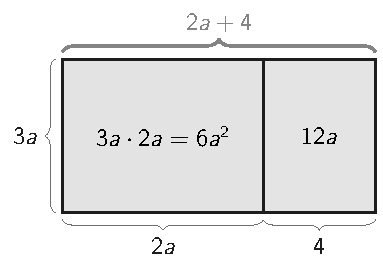
\includegraphics[width=0.95\linewidth]{expr_distributiva}
\end{minipage}
\begin{ojo}[Signos] $(+)(+) = +$, $(-)(-) = +$, $(+)(-) = -$. Así, $-2x(x - 4) = -2x^2 + 8x$. Y al multiplicar se suman exponentes: $x^2\cdot x^3 = x^5$, no $x^6$.\end{ojo}

\subsection{Del lenguaje natural al algebraico}
Lee la frase de afuera hacia adentro: la última operación que se nombra es la que manda. Si la edad de Pedro es $m$, «su edad hace $n$ años disminuida en 3» es $m - n - 3$; «el doble de la suma de un número y 5» es $2(x + 5)$, pero «el doble de un número, más 5» es $2x + 5$.
\begin{center}
\begin{tabular}{@{}ll@{\qquad}ll@{}}
\toprule
En palabras & Expresión & En palabras & Expresión\\ \midrule
el cuadrado de la suma de $a$ y $b$ & $(a + b)^2$ & el triple de la diferencia entre $x$ y 2 & $3(x - 2)$\\
la suma de los cuadrados & $a^2 + b^2$ & dos consecutivos & $n$ y $n + 1$\\
4 menos que $x$ & $x - 4$ & un número par & $2n$\\ \bottomrule
\end{tabular}
\end{center}

\subsection{Perímetros y áreas con expresiones}
Si un rectángulo mide $(2x + 3)$ por $(x - 1)$, su \textbf{perímetro} es $2(2x + 3) + 2(x - 1) = 6x + 4$ y su \textbf{área} es $(2x + 3)(x - 1) = 2x^2 + x - 3$. Con $x = 4$ mide 11 por 3: perímetro 28 y área 33, igual que con las expresiones.
\begin{ojo}[No confundas] El perímetro suma lados (no aparece $x^2$); el área los multiplica. Y para lo que sobra se resta \textbf{todo}, con paréntesis: $(10x + 8) - (6x + 4) = 4x + 4$.\end{ojo}
\gatotip[\gatonaranjo]{¿Dudas entre alternativas? Reemplaza la letra por un número sencillo, como 2, en el enunciado y en cada alternativa: la correcta da lo mismo.}

\begin{elejemplo}{PAES Regular 2026}
Una pista de baile de forma rectangular tiene dimensiones de $(3x + 4)$ metros de largo y $(2x - 9)$ metros de ancho. Se cuenta con $(20x + 20)$ metros de una cinta luminosa para demarcar el borde de la pista de baile.
\begin{center}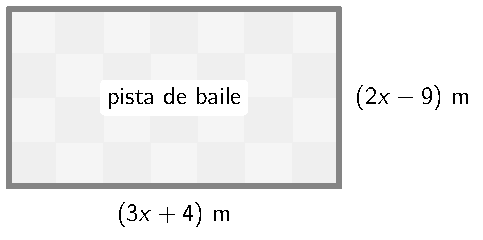
\includegraphics[width=5.2cm]{expr_pista}\end{center}
¿Cuántos metros de cinta luminosa sobran luego de demarcar el borde de la pista?
\alts{$(10x + 30)$ metros}{$(10x + 10)$ metros}{$(15x + 15)$ metros}{$(15x + 25)$ metros}
\solucion{Demarcar el borde es recorrer el perímetro: $2(3x + 4) + 2(2x - 9) = 6x + 8 + 4x - 18 = 10x - 10$. Lo que sobra es la cinta menos todo el perímetro:
\[ (20x + 20) - (10x - 10) = 20x + 20 - 10x + 10 = 10x + 30. \]
Comprobación con $x = 10$: la pista mide 34 m por 11 m, su perímetro es 90 m, la cinta mide 220 m y sobran 130 m $= 10\cdot 10 + 30$. $(10x + 10)$ cambia solo el primer signo del paréntesis; $(15x + 25)$ y $(15x + 15)$ restan medio perímetro.}{A}
\end{elejemplo}

%% =====================================================================
\section{Productos notables}

\subsection{Qué es un producto notable}
Son multiplicaciones tan frecuentes que conviene saber su resultado de memoria. Todas salen de multiplicar término a término, pero reconocer el molde ahorra tiempo y errores de signo.
\begin{clave}[Los cuatro moldes]
\[ (a + b)^2 = a^2 + 2ab + b^2 \qquad (a - b)^2 = a^2 - 2ab + b^2 \]
\[ (a + b)(a - b) = a^2 - b^2 \qquad (x + p)(x + q) = x^2 + (p + q)x + pq \]
Las letras son moldes: en $(2x + 5)^2$, $a = 2x$ y $b = 5$.\end{clave}

\subsection{Cuadrado de binomio}
\begin{minipage}[c]{0.62\linewidth}
En palabras: \textbf{el cuadrado del primero, más (o menos) el doble del primero por el segundo, más el cuadrado del segundo}. El dibujo lo muestra: el cuadrado de lado $a + b$ se parte en $a^2$, $b^2$ y \textbf{dos} rectángulos $ab$.
\[ (x + 5)^2 = x^2 + 10x + 25 \qquad (2x + 3)^2 = 4x^2 + 12x + 9 \]
\[ (x - 4)^2 = x^2 - 8x + 16 \qquad (3x - 2y)^2 = 9x^2 - 12xy + 4y^2 \]
En la resta, el término del medio es negativo y el último \textbf{siempre es positivo}. Además, $(a - b)^2 = (b - a)^2$.
\end{minipage}\hfill
\begin{minipage}[c]{0.34\linewidth}\centering
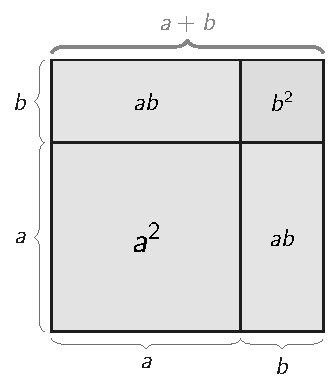
\includegraphics[width=0.85\linewidth]{expr_cuadrado_binomio}
\end{minipage}
\begin{ojo}[El error más común de la PAES] $(a + b)^2 \ne a^2 + b^2$: faltan los dos rectángulos. Con números, $(3 + 4)^2 = 49$, pero $3^2 + 4^2 = 25$. Revisa los tres términos: $(x - 4)^2$ no es $x^2 - 16$, ni $x^2 - 8x - 16$, ni $x^2 - 4x + 16$.\end{ojo}
\gatotip[\gatoatigrado]{Cálculo mental: $21^2 = (20 + 1)^2 = 400 + 40 + 1 = 441$ y $99^2 = (100 - 1)^2 = 10.000 - 200 + 1 = 9801$.}

\subsection{Suma por diferencia}
\begin{minipage}[c]{0.5\linewidth}
Al multiplicar, los términos del medio se cancelan: $(a + b)(a - b) = a^2 - ab + ab - b^2 = a^2 - b^2$. En el dibujo, a un cuadrado de lado $a$ se le quita uno de lado $b$ y lo que queda se reordena en un rectángulo de lados $a + b$ y $a - b$.

$(x + 7)(x - 7) = x^2 - 49$, \quad $(3x + 2y)(3x - 2y) = 9x^2 - 4y^2$ \quad y \quad $103\cdot 97 = 100^2 - 3^2 = 9991$.
\end{minipage}\hfill
\begin{minipage}[c]{0.46\linewidth}\centering
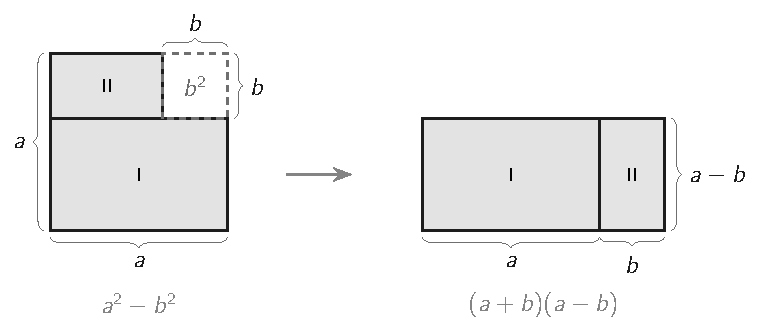
\includegraphics[width=\linewidth]{expr_suma_diferencia}
\end{minipage}
\begin{ojo}[Mismos términos, un signo distinto] $(x + 3)(x - 2)$ no es suma por diferencia.\end{ojo}

\subsection{Binomios con término común}
\begin{minipage}[c]{0.62\linewidth}
En $(x + p)(x + q)$ el resultado es $x^2$, más \textbf{la suma} de los números por $x$, más \textbf{su producto}. En el dibujo, $(x + 4)(x + 3) = x^2 + 7x + 12$.
\[ (x - 5)(x + 2) = x^2 - 3x - 10 \qquad (x - 2)(x - 6) = x^2 - 8x + 12 \]
Si $p = q$ es un cuadrado de binomio; si $q = -p$, una suma por diferencia.
\end{minipage}\hfill
\begin{minipage}[c]{0.34\linewidth}\centering
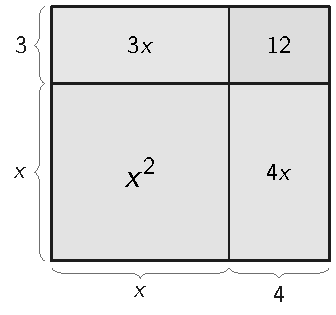
\includegraphics[width=0.8\linewidth]{expr_binomios_comun}
\end{minipage}

\subsection{Combinar productos notables}
Desarrolla cada producto por separado y \textbf{resta con paréntesis}:
\[ (x + 3)^2 - (x + 3)(x - 3) = (x^2 + 6x + 9) - (x^2 - 9) = x^2 + 6x + 9 - x^2 + 9 = 6x + 18. \]
\begin{ejemplo}[Usar datos sin despejar] Si $a + b = 7$ y $ab = 10$: $a^2 + b^2 = (a + b)^2 - 2ab = 49 - 20 = 29$, sin saber cuánto valen $a$ y $b$.\end{ejemplo}
\begin{ojo}[Errores típicos] $(2x)^2 = 4x^2$, no $2x^2$. $(x + 5)^2$ lleva $10x$, no $5x$. $(x + 4)(x - 4) = x^2 - 16$, no $x^2 + 16$. Y al restar $x^2 - 9$, el $-9$ se vuelve $+9$.\end{ojo}
\gatotip[\gatogris]{Comprueba con $x = 1$: la expresión original y tu resultado deben dar el mismo número.}

\begin{elejemplo}{PAES Invierno 2026}
¿Cuál de las siguientes expresiones es igual a $(2x - 3)^2 - (2x - 3)(2x + 3)$?
\alts{$18$}{$0$}{$-6x + 18$}{$-12x + 18$}
\solucion{Cuadrado de binomio con $a = 2x$ y $b = 3$: $(2x - 3)^2 = 4x^2 - 12x + 9$. Suma por diferencia: $(2x - 3)(2x + 3) = 4x^2 - 9$. Restando con paréntesis:
\[ (4x^2 - 12x + 9) - (4x^2 - 9) = 4x^2 - 12x + 9 - 4x^2 + 9 = -12x + 18. \]
Comprobación con $x = 1$: $1 - (-5) = 6$ y $-12 + 18 = 6$. El 18 olvida el término del medio, el 0 cree que los dos productos son iguales y $-6x + 18$ olvida el 2 del doble producto.}{D}
\end{elejemplo}

%% =====================================================================
\section{Factorización}

\subsection{Factorizar es deshacer la multiplicación}
\textbf{Factorizar} es escribir una suma como una multiplicación: el camino inverso de desarrollar. $3a(2a + 4) \to 6a^2 + 12a$ es desarrollar; $6a^2 + 12a \to 6a(a + 2)$ es factorizar. Con números ya lo haces: $12 + 20 = 4(3 + 5)$. Siempre se puede comprobar multiplicando.
\begin{ojo}[Factoriza completo] $3a(2a + 4)$ es igual a $6a^2 + 12a$, pero en el paréntesis queda un 2 común. La factorización completa saca el \textbf{mayor} factor común: $6a(a + 2)$.\end{ojo}

\subsection{Factor común}
\begin{clave}[Cómo encontrarlo] Números: su MCD. Letras: cada letra que está en \textbf{todos} los términos, con su \textbf{menor} exponente. Después divide cada término por el factor común.\end{clave}
\begin{ejemplo} $12x^3 - 18x^2$: MCD 6 y letra $x^2$, así que $12x^3 - 18x^2 = 6x^2(2x - 3)$. Si un término «desaparece» queda 1: $5x + 5 = 5(x + 1)$. El factor común puede ser un paréntesis: $x(a + b) + 3(a + b) = (a + b)(x + 3)$.\end{ejemplo}
\gatotip[\gatonegro]{Cálculo mental: $37\cdot 13 + 37\cdot 87 = 37(13 + 87) = 3700$. El 37 sale una sola vez.}

\subsection{Diferencia de cuadrados}
\begin{clave} \[ a^2 - b^2 = (a + b)(a - b) \] Dos cuadrados separados por un menos. Se usan sus \textbf{raíces}.\end{clave}
\begin{ejemplo} $x^2 - 49 = (x + 7)(x - 7)$; $9x^2 - 16y^2 = (3x + 4y)(3x - 4y)$; $2x^2 - 50 = 2(x^2 - 25) = 2(x + 5)(x - 5)$; $51^2 - 49^2 = 100\cdot 2 = 200$.\end{ejemplo}
\begin{ojo}[La suma de cuadrados no se factoriza así] $x^2 + 9$ no es $(x + 3)(x - 3)$, que da $x^2 - 9$, ni $(x + 3)^2$, que da $x^2 + 6x + 9$.\end{ojo}

\subsection{Trinomio cuadrado perfecto}
\begin{clave} \[ a^2 + 2ab + b^2 = (a + b)^2 \qquad a^2 - 2ab + b^2 = (a - b)^2 \] Los extremos son cuadrados positivos; saca sus raíces; el término del medio debe ser el \textbf{doble} de su producto, y su signo dice si es suma o resta.\end{clave}
\begin{ejemplo} $x^2 + 10x + 25$: raíces $x$ y 5, y $2\cdot x\cdot 5 = 10x$: es $(x + 5)^2$. $4x^2 - 12x + 9 = (2x - 3)^2$. En cambio, $x^2 + 6x + 25$ no es cuadrado perfecto: el medio debería ser $10x$.\end{ejemplo}

\subsection{Trinomio x² + bx + c}
\begin{minipage}[c]{0.64\linewidth}
\[ x^2 + bx + c = (x + p)(x + q) \quad\text{con}\quad p + q = b,\ \ pq = c \]
Busca \textbf{dos números que multiplicados den $c$ y sumados den $b$}. En $x^2 + 7x + 12$ son 3 y 4: $(x + 3)(x + 4)$, el rectángulo del dibujo.
\begin{clave}[Regla de signos] Si $c$ es positivo, los dos números tienen el signo de $b$: $x^2 - 9x + 20 = (x - 4)(x - 5)$. Si $c$ es negativo, tienen signos distintos: $x^2 - 2x - 15 = (x - 5)(x + 3)$.\end{clave}
\end{minipage}\hfill
\begin{minipage}[c]{0.32\linewidth}\centering
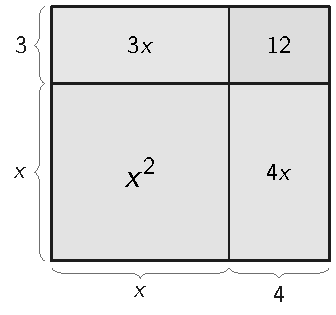
\includegraphics[width=0.85\linewidth]{expr_binomios_comun}
\end{minipage}

\subsection{Simplificar fracciones algebraicas}
Solo se tachan \textbf{factores} (cosas que multiplican), nunca sumandos. Por eso primero se factoriza:
\[ \frac{x^2 - 9}{x + 3} = \frac{(x + 3)(x - 3)}{x + 3} = x - 3 \ \ (x \ne -3), \qquad \frac{x^2 + 5x}{x^2 - 25} = \frac{x(x + 5)}{(x + 5)(x - 5)} = \frac{x}{x - 5}. \]
El valor que anula el denominador original queda excluido también después de simplificar.
\begin{ojo}[Así no] $\dfrac{x + 6}{x + 2} \ne \dfrac{6}{2}$. Con $x = 2$ vale $\dfrac{8}{4} = 2$, no 3.\end{ojo}

\subsection{Qué factorización uso}
\begin{center}
\small\begin{tabular}{@{}lll@{}}
\toprule
Mira esto & Usa & Ejemplo\\ \midrule
algo se repite en todos los términos & factor común (siempre primero) & $4x^2 + 6x = 2x(2x + 3)$\\
dos cuadrados con un menos & diferencia de cuadrados & $x^2 - 36 = (x + 6)(x - 6)$\\
extremos cuadrados y medio $2ab$ & trinomio cuadrado perfecto & $x^2 - 8x + 16 = (x - 4)^2$\\
$x^2 + bx + c$ & producto $c$, suma $b$ & $x^2 + x - 12 = (x + 4)(x - 3)$\\ \bottomrule
\end{tabular}
\end{center}
Después revisa si algún paréntesis se puede factorizar de nuevo: $3x^2 - 12 = 3(x + 2)(x - 2)$ y $2x^3 - 8x^2 + 8x = 2x(x - 2)^2$. Si un producto vale 0, algún factor vale 0: $(p - 3)^2 - 36 = (p + 3)(p - 9) = 0$ da $p = -3$ o $p = 9$.
\gatotip[\gatolila]{Con un área y un lado, factoriza el área: si mide $x^2 + 7x + 12$ y un lado es $x + 3$, el otro es $x + 4$. Y descarta las medidas negativas.}

\begin{elejemplo}{PAES Regular 2026, adaptada}
Una persona realiza el siguiente procedimiento para factorizar $12x^2 + 20x$, cometiendo un error.

Paso 1: escribe cada término como un producto, obteniendo $4\cdot 3\cdot x\cdot x + 4\cdot 5\cdot x$.\\
Paso 2: descompone cada número en factores primos, obteniendo $2\cdot 2\cdot 3\cdot x\cdot x + 2\cdot 2\cdot 5\cdot x$.\\
Paso 3: escribe las potencias correspondientes, obteniendo $2^2\cdot 3\cdot x^2 + 2^2\cdot 5\cdot x$.\\
Paso 4: factoriza la suma, obteniendo $2^4x(3x + 5)$.

¿En cuál de los pasos la persona cometió el error?
\alts{En el Paso 1}{En el Paso 2}{En el Paso 3}{En el Paso 4}
\solucion{Los Pasos 1, 2 y 3 solo reescriben los números: cada expresión sigue siendo igual a $12x^2 + 20x$. En el Paso 4, el factor común es lo que se repite en los dos términos, $2^2$ y $x$, o sea $4x$; la persona sumó los exponentes de los dos $2^2$ y escribió $2^4 = 16$. Lo que se repite se saca \textbf{una vez}. Lo correcto es $12x^2 + 20x = 4x(3x + 5)$; en cambio, $2^4x(3x + 5) = 48x^2 + 80x$, el cuádruple de lo pedido.}{D}
\end{elejemplo}

%% =====================================================================
\section{Proporcionalidad directa}

\subsection{Razón y proporción}
Una \textbf{razón} compara dos cantidades dividiéndolas: 12 niñas y 18 niños están en la razón $12 : 18 = \frac{12}{18} = 2 : 3$, es decir, por cada 2 niñas hay 3 niños. Una \textbf{proporción} es una igualdad de razones, como $\frac{2}{3} = \frac{8}{12}$.
\begin{clave}[Propiedad fundamental] $\dfrac{a}{b} = \dfrac{c}{d}$ es lo mismo que $a\cdot d = b\cdot c$ (producto cruzado). Con ella se despeja el término que falta: $\dfrac{x}{15} = \dfrac{2}{3} \Rightarrow 3x = 30 \Rightarrow x = 10$.\end{clave}
\begin{ojo}[El orden importa] Cuando dice \textbf{respectivamente}, el primer número va con lo primero que se nombra. Y si la razón es $2 : 3$, el grupo tiene $2 + 3 = 5$ partes: las niñas son $\frac{2}{5}$ del curso, no $\frac{2}{3}$.\end{ojo}

\subsection{Qué es la proporcionalidad directa}
Dos cantidades son \textbf{directamente proporcionales} si, cuando una se multiplica por un número, la otra se multiplica por el \textbf{mismo} número: el doble con el doble, la mitad con la mitad. El cociente es constante:
\begin{clave} \[ \frac{y}{x} = k \qquad\Longleftrightarrow\qquad y = k\cdot x \] La constante $k$ es lo que vale $y$ cuando $x = 1$: el precio de \textbf{un} cuaderno, lo que se paga por \textbf{un} minuto. Se llama valor unitario.\end{clave}
\begin{center}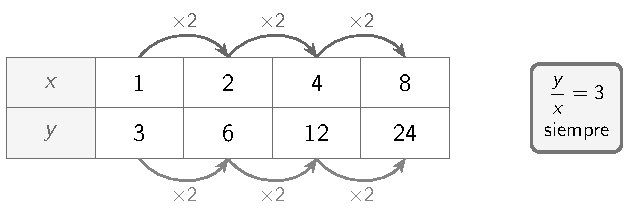
\includegraphics[width=8.2cm]{prop_tabla_directa}\end{center}
\textbf{En una tabla}, divide $y$ por $x$ en cada columna: con $x$: 2, 5, 8 e $y$: 6, 15, 24 siempre da 3, así que es directa. Con $x$: 1, 2, 3 e $y$: 5, 7, 9 da 5; 3,5 y 3: no lo es (es $y = 2x + 3$).
\begin{ojo}[Que las dos crezcan no basta] Al pasar de $x = 1$ a $x = 2$, $y$ debe duplicarse. Además, si $x = 0$, entonces $y = 0$: con un cobro fijo (la bajada de bandera de un taxi) ya no es proporcional.\end{ojo}

\subsection{El gráfico: una recta que pasa por el origen}
\begin{minipage}[c]{0.5\linewidth}
Los puntos $(x, y)$ de $y = kx$ quedan sobre una recta que pasa por $(0, 0)$. Para leer $k$, toma un punto distinto del origen y divide su altura por su $x$: con $(4, 12)$, $k = 3$. Cada vez que avanzas 1, la recta sube $k$: $k$ es la pendiente.

En cambio, $y = 3x + 2$ también es una recta, pero corta el eje $Y$ en 2: no es proporcionalidad directa.
\end{minipage}\hfill
\begin{minipage}[c]{0.46\linewidth}\centering
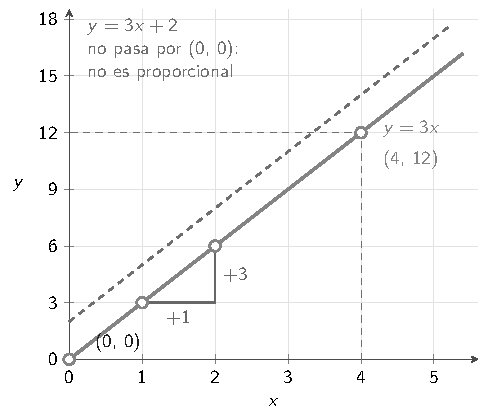
\includegraphics[width=0.92\linewidth]{prop_graf_directa}
\end{minipage}

\subsection{La regla de tres directa}
\begin{ejemplo} 4 kg de paltas cuestan \peso 7200; ¿cuánto cuestan 6 kg? \textbf{Valor unitario:} 1 kg cuesta $\frac{7200}{4} = 1800$, y 6 kg, $6\cdot 1800 = 10.800$. \textbf{Proporción:} $\frac{4}{7200} = \frac{6}{x}$, así que $4x = 43.200$ y $x = 10.800$.\end{ejemplo}
\begin{ojo}[Revisa el sentido] Kilos arriba y pesos abajo en las dos razones. Si te da que 6 kg cuestan menos que 4 kg, armaste mal la proporción. Y si una cantidad aumenta en 100, la otra no aumenta en 100: aumenta en la misma \textbf{proporción}.\end{ojo}
\gatotip[\gatoblanco]{Las escalas de mapas son proporción directa: si 1 cm equivale a 50 m, 7 cm son $7\cdot 50 = 350$ m. Calcula primero lo que vale 1 cm.}

\subsection{Repartos proporcionales}
\begin{clave}[Repartir en la razón $a : b$] Cuenta las partes, $a + b$; divide el total por ese número para obtener una parte, y multiplica por las partes de cada uno.\end{clave}
\begin{ejemplo} \peso 60.000 en la razón $2 : 3$: son 5 partes de 12.000; Ana recibe 24.000 y Beto 36.000. Si se reparte según lo que aportó cada uno (\peso 3000 y \peso 2000), la razón es $3 : 2$.\end{ejemplo}
\begin{ojo}[No dividas por 2] Repartir en la razón $2 : 3$ no es repartir por mitades, ni dividir por 2 y por 3: se divide por el total de partes, 5.\end{ojo}

\begin{elejemplo}{PAES Invierno 2026, adaptada}
Javier y David compraron una bolsa de 24 dulces a un precio total de \peso 2100, tal que Javier aportó \peso 1400 y David aportó el resto del dinero.

Ellos deciden vender cada dulce a \peso 200 y repartirse el dinero obtenido de forma proporcional a lo que aportó cada uno en la compra.

¿Cuánto dinero recibirá Javier luego de vender todos los dulces?
\alts{\peso 1600}{\peso 2400}{\peso 2700}{\peso 3200}
\solucion{La venta da $24\cdot 200 = 4800$ pesos. David aportó $2100 - 1400 = 700$, así que los aportes están en la razón $1400 : 700 = 2 : 1$. Son $2 + 1 = 3$ partes de $\frac{4800}{3} = 1600$, y Javier recibe 2 partes: $3200$ pesos. Comprobación: David recibe 1600 y $3200 + 1600 = 4800$. \peso 1600 es lo de David, \peso 2400 reparte por mitades y \peso 2700 es la ganancia total.}{D}
\end{elejemplo}

%% =====================================================================
\section{Proporcionalidad inversa}

\subsection{Qué es la proporcionalidad inversa}
Dos cantidades son \textbf{inversamente proporcionales} si, cuando una se multiplica por un número, la otra se \textbf{divide} por ese mismo número: si una se duplica, la otra se reduce a la mitad. Al repartir 24 caramelos entre 1, 2, 4 u 8 niños tocan 24, 12, 6 o 3: el producto siempre es 24.
\begin{clave} \[ x\cdot y = k \qquad\Longleftrightarrow\qquad y = \frac{k}{x} \] La constante $k$ es el total: lo que se reparte, la distancia del viaje, el trabajo de la obra.\end{clave}
\begin{center}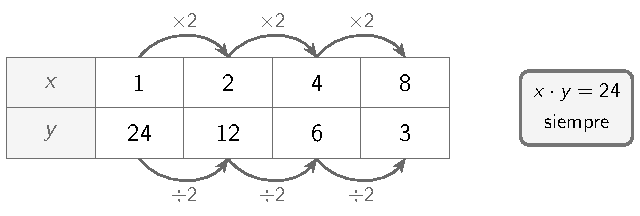
\includegraphics[width=8.2cm]{prop_tabla_inversa}\end{center}

\subsection{Cómo reconocerla}
En una tabla, \textbf{multiplica} $x$ por $y$ en cada columna. A 60 km/h se tarda 4 h, a 80 km/h 3 h y a 120 km/h 2 h: el producto es siempre 240 (la distancia), así que es inversa. Con $x$: 1, 2, 3 e $y$: 10, 8, 6 los productos son 10, 16 y 18: no lo es.
\begin{center}
\begin{tabular}{@{}lll@{}}
\toprule
 & Directa & Inversa\\ \midrule
lo constante & $\dfrac{y}{x} = k$ & $x\cdot y = k$\\[6pt]
fórmula & $y = kx$ & $y = \dfrac{k}{x}$\\[6pt]
si $x$ se duplica & $y$ se duplica & $y$ se divide por 2\\
gráfico & recta por el origen & hipérbola\\ \bottomrule
\end{tabular}
\end{center}
\begin{ojo}[Que una baje cuando la otra sube no basta] En $y = 10 - x$, $y$ baja, pero $1\cdot 9 = 9$ y $2\cdot 8 = 16$. Revisa \textbf{todas} las columnas.\end{ojo}

\subsection{El gráfico: una hipérbola}
\begin{minipage}[c]{0.5\linewidth}
Los puntos de $y = \frac{24}{x}$ forman una curva llamada \textbf{hipérbola}: cuando $x$ crece, $y$ baja, primero rápido y después cada vez más lento. Se acerca a los ejes pero \textbf{nunca los toca}, porque $x$ e $y$ no pueden valer 0.

Desde el origen hasta cada punto se forma un rectángulo de área $x\cdot y = 24$: todos tienen la misma área.
\end{minipage}\hfill
\begin{minipage}[c]{0.46\linewidth}\centering
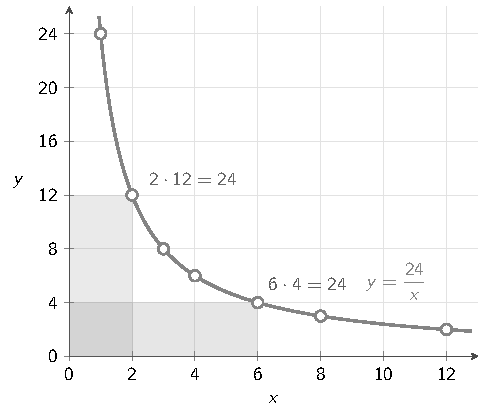
\includegraphics[width=0.92\linewidth]{prop_graf_inversa}
\end{minipage}

\subsection{Trabajadores, rapidez, raciones y llaves}
\begin{clave}[Método] 1. ¿Más de una da menos de la otra? 2. Calcula $k = x\cdot y$, el total. 3. Divide $k$ por la nueva cantidad. 4. Revisa el sentido.\end{clave}
\begin{ejemplo}[Trabajadores] 6 obreros tardan 10 días: la obra son $6\cdot 10 = 60$ «días de un obrero». Con 4 obreros: $\frac{60}{4} = 15$ días. Con proporción, sin dar vuelta nada: $6\cdot 10 = 4\cdot x$.\end{ejemplo}
\begin{ejemplo}[Rapidez, raciones y llaves] A 90 km/h se tarda 4 h: son 360 km, y a 120 km/h se tarda 3 h. Comida para 20 personas por 15 días son 300 raciones: con 25 personas alcanza para 12 días. 3 llaves llenan un estanque en 8 h: son 24 «horas de una llave», y con 4 llaves se tarda 6 h.\end{ejemplo}
\begin{ojo}[El error más común] Hacer regla de tres directa: $\frac{6}{10} = \frac{4}{x}$ da 6,7 días, como si con menos obreros se terminara antes. Todo esto supone el mismo ritmo, que la PAES indica con frases como «en las mismas condiciones».\end{ojo}

\subsection{Dos proporciones a la vez}
Si cambian tres cantidades, ve al \textbf{valor de una unidad}. 4 trabajadores llenan 2000 cajas en 20 días: los 4 llenan $\frac{2000}{20} = 100$ cajas diarias y uno solo, $\frac{100}{4} = 25$. Para 32.000 cajas en 10 días se necesitan 3200 diarias, o sea $\frac{3200}{25} = 128$ trabajadores.
\gatotip[\gatonaranjo]{Lo que hace \emph{uno} se obtiene \emph{dividiendo} lo que hacen todos. Un solo trabajador no puede llenar más cajas que los cuatro juntos.}

\subsection{Directa, inversa o ninguna}
\begin{center}
\begin{tabular}{@{}lll@{}}
\toprule
Situación & Al duplicar $x$ & Tipo\\ \midrule
kilos de pan y precio a pagar & el precio se duplica & directa\\
rapidez y tiempo de un mismo viaje & el tiempo se reduce a la mitad & inversa\\
personas y porción de una torta & la porción se reduce a la mitad & inversa\\
minutos y cobro con cargo fijo & aumenta, pero no al doble & ninguna\\
edad y estatura & no hay regla fija & ninguna\\ \bottomrule
\end{tabular}
\end{center}
\gatotip[\gatogris]{$k$ no es la respuesta: si $x\cdot y = 60$ y $x = 5$, la respuesta es $y = 12$, no 60.}

\begin{elejemplo}{PAES Invierno 2027, adaptada}
En una empresa hay 4 trabajadores para cosechar uvas y estos logran llenar 2000 cajas en 20 días de trabajo, todos trabajando todos los días, al mismo ritmo y la misma cantidad de horas.

En la empresa se realiza el siguiente procedimiento para calcular la cantidad de trabajadores necesarios para llenar 32.000 cajas en 10 días, bajo las mismas condiciones, cometiéndose un error.

Paso 1: se calcula la cantidad de cajas que llenan diariamente los 4 trabajadores en conjunto como $\frac{2000}{20}$, obteniéndose que llenan 100 cajas diarias.\\
Paso 2: se calcula la cantidad de cajas que cada trabajador llena diariamente como $100\cdot 4$, obteniéndose 400 cajas diarias por trabajador.\\
Paso 3: se calcula la cantidad de cajas que se deben llenar diariamente para la nueva producción como $\frac{32.000}{10}$, obteniéndose 3200 cajas diarias.\\
Paso 4: se divide la cantidad de cajas diarias que se deben llenar por la cantidad que cada trabajador llena diariamente como $\frac{3200}{400}$, obteniéndose que se necesitan 8 trabajadores.

¿En cuál de los pasos se cometió el error?
\alts{En el Paso 1}{En el Paso 2}{En el Paso 3}{En el Paso 4}
\solucion{El Paso 1 está bien: $\frac{2000}{20} = 100$ cajas diarias entre los 4. En el Paso 2 está el error: lo que llena \textbf{uno} es $\frac{100}{4} = 25$ cajas diarias; se multiplicó por 4 en vez de dividir. El Paso 3 está bien ($\frac{32.000}{10} = 3200$) y el Paso 4 tiene la idea correcta, pero arrastra el 400. Lo correcto: $\frac{3200}{25} = 128$ trabajadores, que llenan $128\cdot 25 = 3200$ cajas diarias.}{B}
\end{elejemplo}

%% =====================================================================
\section{Sistemas de ecuaciones lineales}

\subsection{Qué es un sistema de ecuaciones}
Un \textbf{sistema} son dos ecuaciones con las mismas dos incógnitas que se deben cumplir \textbf{al mismo tiempo}. Su \textbf{solución} es el par $(x, y)$ que hace verdaderas \textbf{las dos}:
\[ \begin{cases} x + y = 10 \\ x - y = 4 \end{cases} \qquad\text{solución } (7, 3):\quad 7 + 3 = 10,\ \ 7 - 3 = 4. \]
\begin{ojo}[Las dos, no una] $(6, 4)$ cumple la primera, pero no la segunda: no es solución. Y en el par va primero la $x$: $(3, 7)$ es otro par.\end{ojo}

\subsection{Los tres métodos}
\begin{clave}[Sustitución] Despeja una incógnita y \textbf{reemplázala con paréntesis} en la otra ecuación. Conviene cuando una letra tiene coeficiente 1 o $-1$.\end{clave}
\begin{ejemplo} $2x + y = 11$ y $x - 3y = -5$: $y = 11 - 2x$, y $x - 3(11 - 2x) = -5$ da $7x - 33 = -5$, o sea $x = 4$ e $y = 3$.\end{ejemplo}
\begin{clave}[Igualación] Despeja la misma incógnita en las dos e iguala. Conviene cuando las dos vienen como $y = \dots$\end{clave}
\begin{ejemplo} $y = 2x + 1$ e $y = -x + 7$: $2x + 1 = -x + 7$, así que $x = 2$ e $y = 5$.\end{ejemplo}
\begin{clave}[Reducción] Suma las ecuaciones para que una incógnita desaparezca; si hace falta, antes multiplica \textbf{toda} una ecuación. Conviene con coeficientes opuestos.\end{clave}
\begin{ejemplo} $2x + 3y = 12$ y $3x - y = 7$: la segunda por 3 es $9x - 3y = 21$; sumando, $11x = 33$, $x = 3$ e $y = 2$.\end{ejemplo}
\begin{ojo}[Errores típicos] Reemplazar sin paréntesis ($x - 3\cdot 11 - 2x$); multiplicar solo un lado ($9x - 3y = 7$); quedarse con una incógnita o dar vuelta el par. Con fracciones, multiplica antes la ecuación por el mcm.\end{ojo}
\gatotip[\gatoatigrado]{Si te quedas en blanco, reemplaza cada alternativa en las \emph{dos} ecuaciones: la correcta cumple ambas. Y si te dan la solución con letras $a$ y $b$, reemplázala para encontrarlas.}

\subsection{Una, ninguna o infinitas soluciones}
Cada ecuación lineal es una \textbf{recta} y la solución del sistema es el punto donde se cortan (por ejemplo, $x + y = 5$ y $x - y = 1$ se cortan en $(3, 2)$). Dos rectas pueden estar de tres maneras:
\begin{center}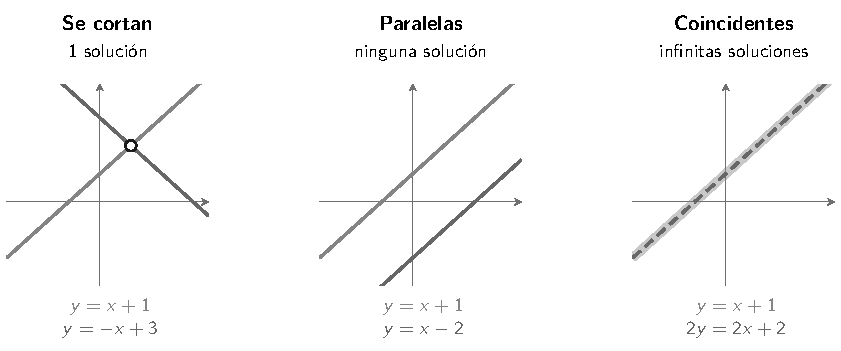
\includegraphics[width=0.85\linewidth]{sis_tres_casos}\end{center}
\begin{center}
\begin{tabular}{@{}llll@{}}
\toprule
Rectas & Despejando $y$ & Soluciones & Al resolver queda\\ \midrule
se cortan & distinta pendiente & una & $x$ e $y$\\
paralelas & misma pendiente, distinto corte & ninguna & algo falso, como $0 = -2$\\
coincidentes & todo igual & infinitas & $0 = 0$\\ \bottomrule
\end{tabular}
\end{center}
\begin{ejemplo} $x + 2y = 3$ y $x + 2y = 5$ son paralelas. $x + 2y = 3$ y $2x + 4y = 6$ son la misma recta: la segunda es la primera multiplicada por 2 en \textbf{todos} sus términos.\end{ejemplo}
\begin{ojo}[Nunca dos] Dos rectas distintas no se cortan en exactamente dos puntos.\end{ojo}

\begin{elejemplo}{Tipo PAES}
¿Cuál es la solución del siguiente sistema de ecuaciones?
\[ \begin{cases} 3x - 2y = 5 \\ x + 4y = 11 \end{cases} \]
\alts{$(2, 3)$}{$(1, -1)$}{$(3, 2)$}{$(7, 1)$}
\solucion{En la segunda la $x$ tiene coeficiente 1: sustitución. $x = 11 - 4y$, y en la primera, $3(11 - 4y) - 2y = 5$, o sea $33 - 14y = 5$, $-14y = -28$ e $y = 2$. Entonces $x = 11 - 8 = 3$. Comprobación: $9 - 4 = 5$ y $3 + 8 = 11$. $(2, 3)$ da vuelta el par, $(1, -1)$ solo cumple la primera y $(7, 1)$ solo la segunda.}{C}
\end{elejemplo}

%% =====================================================================
\section{Problemas con sistemas de ecuaciones}

\subsection{Del enunciado al sistema en 4 pasos}
\begin{clave}[Los 4 pasos] 1. Nombra las dos incógnitas, con su unidad. 2. Escribe una ecuación por cada dato total: casi siempre uno de \textbf{cantidades} y otro de \textbf{valor}. 3. Resuelve. 4. Responde y comprueba en el enunciado.\end{clave}
\begin{ejemplo}[Entradas] Adulto \peso 5000, niño \peso 3000; 80 entradas y \peso 300.000: $x + y = 80$ y $5000x + 3000y = 300.000$. Con $y = 80 - x$ se llega a $2000x = 60.000$: 30 de adulto y 50 de niño.\end{ejemplo}
\begin{ojo}[No mezcles] En la ecuación de cantidades no van precios, y en la de dinero cada cantidad va con \textbf{su} precio. $x + y = 300.000$ no tiene sentido: suma entradas y da pesos.\end{ojo}

\subsection{Monedas, edades y mezclas}
\begin{ejemplo}[Monedas] 30 monedas de \peso 100 y \peso 500 suman \peso 7400: $x + y = 30$ y $100x + 500y = 7400$. Dividiendo la segunda por 100, $x + 5y = 74$; restando la primera, $4y = 44$: 11 de 500 y 19 de 100.\end{ejemplo}
\begin{ejemplo}[Edades] Padre e hijo suman 50; hace 5 años el padre tenía 4 veces la edad del hijo: $p + h = 50$ y $p - 5 = 4(h - 5)$. Resulta $h = 13$ y $p = 37$.\end{ejemplo}
\begin{ojo}[Paréntesis en las edades] «4 veces la edad del hijo hace 5 años» es $4(h - 5)$, no $4h - 5$. Y el tiempo pasa para todos: en 4 años, $a + 4 = 3(h + 4)$.\end{ojo}
\begin{ejemplo}[Mezclas] Café de \peso 8000 y de \peso 12.000 el kilo para 20 kg a \peso 9000: $x + y = 20$ y $8000x + 12.000y = 20\cdot 9000$. Resulta 15 kg del barato y 5 kg del caro: el precio de la mezcla está más cerca del café barato.\end{ejemplo}
\gatotip[\gatolila]{Si el precio es «por kilogramo», la incógnita son \emph{kilogramos}, no frutas ni paquetes. La PAES pregunta justo eso.}

\subsection{Planes: ¿cuándo cuestan lo mismo?}
\begin{minipage}[c]{0.5\linewidth}
Plan A: \peso 8000 más \peso 50 por minuto; plan B: \peso 12.000 más \peso 30. Igualando, $8000 + 50m = 12.000 + 30m$: $m = 200$ minutos, con un costo de \peso 18.000 en ambos.

El punto donde se cortan las rectas es donde las dos cantidades valen lo mismo. Antes de 200 minutos conviene A; después, B.
\end{minipage}\hfill
\begin{minipage}[c]{0.46\linewidth}\centering
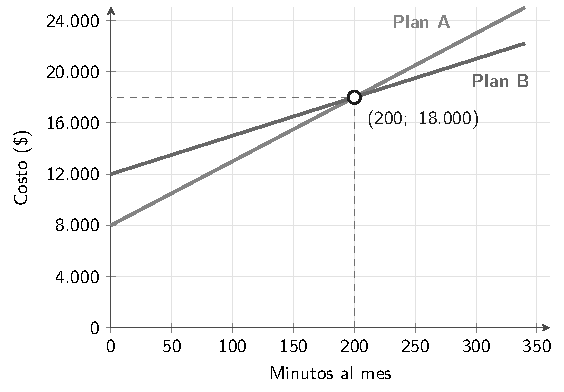
\includegraphics[width=\linewidth]{sis_planes}
\end{minipage}
\begin{ejemplo}[Tarifa fija] Con \peso 2300 por 40 minutos y \peso 3800 por 70: $f + 40v = 2300$ y $f + 70v = 3800$. Restando, $30v = 1500$: $v = 50$ y la tarifa fija es $f = 300$.\end{ejemplo}

\subsection{Qué representa cada parte del sistema}
En una obra de teatro la entrada de niño cuesta \peso 2000 y la de adulto \peso 3500; una familia pagó \peso 40.000 por 14 entradas:
\[ \begin{cases} x + y = 14 \\ 2000x + 3500y = 40.000 \end{cases} \]
\begin{clave}[Cantidad, precio o dinero] $x$ va con 2000: es la \textbf{cantidad} de entradas de niño. 2000 es un \textbf{precio}. $2000x$ es \textbf{dinero}: lo pagado por las entradas de niño. 40.000 es el total pagado y 14 el total de entradas.\end{clave}
\begin{ojo}[Porcentajes] Si aparece $\frac{80}{100}\cdot B$ como lo pagado con un 20~\% de descuento, $B$ es el precio \textbf{original}. Y no sumes lo que el enunciado excluye: «se recaudó solo por las poleras» deja fuera los envíos.\end{ojo}
\gatotip[\gatonegro]{Al final, relee qué representa cada letra: si piden las entradas de niño y respondes $y$, marcaste la otra.}

\begin{elejemplo}{PAES Invierno 2026, adaptada}
Una empresa dedicada a la venta de poleras ofrece a sus clientes dos opciones de diseño: personalizado o de catálogo. El precio por polera con diseño personalizado es \peso 8500 y con diseño de catálogo es \peso 7500. Adicionalmente, se hace un cobro por envío a domicilio de \peso 2500.

En un día de trabajo se vendió un total de 18 poleras en diez envíos y se recaudó \peso 146.000 solo por las poleras. Para calcular la cantidad de poleras con diseño personalizado que se vendieron, una persona realiza el siguiente procedimiento, cometiendo un error.

Paso 1: representa con $x$ la cantidad de poleras con diseño personalizado y con $y$ la cantidad de poleras con diseño de catálogo, y establece el sistema $\begin{cases} x + y = 18 \\ 8500x + 7500y = 146.000 + 25.000 \end{cases}$\\[2pt]
Paso 2: despeja $y$ de la primera ecuación, obteniendo $y = 18 - x$.\\
Paso 3: reemplaza $y$ en la segunda ecuación, obteniendo $8500x - 7500x = 146.000 + 25.000 - 7500\cdot 18$.\\
Paso 4: resuelve la igualdad anterior y determina que la cantidad de poleras con diseño personalizado es 36.

¿En cuál de los pasos la persona cometió el error?
\alts{En el Paso 1}{En el Paso 2}{En el Paso 3}{En el Paso 4}
\solucion{La primera ecuación está bien, pero en la segunda $8500x + 7500y$ es el dinero de las poleras, y el enunciado dice que se recaudaron 146.000 \textbf{solo por las poleras}: los $10\cdot 2500 = 25.000$ de los envíos no van ahí. El error está en el Paso 1. Los Pasos 2, 3 y 4 operan bien con lo que reciben. Lo correcto: $1000x = 146.000 - 135.000 = 11.000$, o sea 11 personalizadas y 7 de catálogo; $8500\cdot 11 + 7500\cdot 7 = 146.000$. Además, 36 poleras personalizadas es imposible si en total se vendieron 18.}{A}
\end{elejemplo}

\chapter{Funciones}
%% Estilo común de los gráficos del capítulo (rectas y parábolas pequeñas).
\pgfplotsset{capfun/.style={width=6.4cm,height=5cm,axis lines=middle,xlabel={$x$},ylabel={$y$},
  every axis x label/.style={at={(ticklabel* cs:1)},anchor=west,font=\small},
  every axis y label/.style={at={(ticklabel* cs:1)},anchor=south,font=\small},
  tick label style={font=\scriptsize},grid=major,grid style={gris!20},samples=120,
  every axis plot/.append style={line width=1.1pt}}}

%% =====================================================================
\section{Concepto de función}
%% =====================================================================

\subsection{Qué es una función}
Una \textbf{función} es una regla que a cada número que entra le asigna \textbf{un solo} número que sale. Al que entra lo llamamos $x$ y al que sale, $f(x)$ («f de x»).
\begin{itemize}
  \item \textbf{Variable independiente}: la $x$, lo que tú eliges.
  \item \textbf{Variable dependiente}: $y = f(x)$, lo que sale; depende de la $x$.
  \item \textbf{Dominio}: los valores que puede tomar la $x$. Si no se dice nada, son todos los números reales.
\end{itemize}
\begin{ejemplo} El kilo de pan cuesta \peso 2.000. Si compro $x$ kilos, pago $f(x) = 2.000\cdot x$. Con 2 kilos: $f(2) = 2.000\cdot 2 = 4.000$ pesos.\end{ejemplo}
\begin{ojo}[Ojo con la escritura] $f(2)$ no es «f por 2»: es lo que sale cuando entra el 2.\end{ojo}

\subsection{Una sola salida para cada entrada}
Un par $(x, y)$ dice «entra $x$, sale $y$». Para que un conjunto de pares sea función, ninguna $x$ puede tener dos salidas distintas.
\begin{clave}[La regla de oro] Dos entradas con la misma salida, como $(1, 5)$ y $(2, 5)$: \textbf{permitido}. Una entrada con dos salidas, como $(1, 5)$ y $(1, 7)$: \textbf{no es función}.\end{clave}
\begin{ejemplo} En $\{(2, 3),\ (5, 3),\ (2, 8)\}$ la entrada $2$ sale una vez $3$ y otra vez $8$: no es función.\end{ejemplo}
En un gráfico se usa una \textbf{recta vertical}: si en algún lugar corta la curva en dos puntos o más, no es función. Una recta horizontal sí puede cortarla varias veces.

\subsection{Evaluar: reemplazar la x}
Evaluar es cambiar \textbf{cada} $x$ de la fórmula por el número, \textbf{entre paréntesis}, y calcular respetando el orden: potencias, multiplicaciones, sumas.
\begin{ejemplo} Si $f(x) = 2x^2 - 7x + 1$:
$f(-3) = 2(-3)^2 - 7(-3) + 1 = 2\cdot 9 + 21 + 1 = 40$.\end{ejemplo}
\begin{ojo}[Tres trampas]
\begin{itemize}
  \item $(-3)^2 = 9$, pero $-3^2 = -(3\cdot 3) = -9$.
  \item $-x^2$ significa $-(x^2)$: si $g(x) = -x^2 + 10$, entonces $g(-3) = -9 + 10 = 1$, no $19$.
  \item $f(2) + f(3)$ no es $f(5)$: con $f(x) = 4x - 1$, $f(2) + f(3) = 7 + 11 = 18$, pero $f(5) = 19$.
\end{itemize}
\end{ojo}
\gatotip[\gatogris]{Reemplaza siempre con paréntesis, aunque el número sea positivo. Con los negativos es lo que te salva: menos por menos da más.}

\subsection{Imagen y preimagen}
Si $f(a) = b$, decimos que $b$ es la \textbf{imagen} de $a$ y que $a$ es una \textbf{preimagen} de $b$.
\begin{clave}[¿Evaluar o despejar?] Si te dan la $x$, \textbf{evalúa}. Si te dan el resultado, \textbf{iguala} la fórmula a ese resultado y despeja la $x$.\end{clave}
\begin{ejemplo} Si $g(x) = 4x + 6$, la preimagen de $26$ sale de $4x + 6 = 26$: $4x = 20$ y $x = 5$. Comprobación: $g(5) = 26$ \checkmark.\end{ejemplo}
Un número puede tener dos preimágenes o ninguna: si $h(x) = x^2$, el $9$ tiene dos ($3$ y $-3$), y el $-4$ no tiene ninguna, porque un cuadrado nunca es negativo. Si en la fórmula falta una constante, un dato como $f(2) = 11$ se convierte en una ecuación para encontrarla.

\subsection{Funciones en tablas y gráficos}
En una tabla, cada fila es un par (entrada, salida). Una fórmula corresponde a la tabla solo si calza en \textbf{todas} las filas. Si la $x$ sube de 1 en 1 y $f(x)$ sube siempre lo mismo, prueba «salto por $x$ más el valor en $x = 0$».

En un gráfico, la entrada se lee en el eje $X$ y la salida es la \textbf{altura}:
\begin{itemize}
  \item $f(a)$: desde $x = a$ sube (o baja) hasta la curva y lee la altura.
  \item $f(x) = b$: traza una horizontal a altura $b$ y, desde cada corte, baja a leer la $x$.
\end{itemize}
\begin{center}
\begin{tikzpicture}
\begin{axis}[capfun,xmin=-3,xmax=3,ymin=-1,ymax=9,xtick={-3,...,3},ytick={0,2,...,8}]
  \addplot[nar,domain=-3:3] {x^2};
  \addplot[azul,dashed,line width=0.8pt,domain=-3:3] {4};
  \draw[menta,dashed,line width=0.8pt] (axis cs:2,0) -- (axis cs:2,4);
  \addplot[only marks,mark=*,mark size=2pt,nard] coordinates {(2,4) (-2,4)};
  \node[font=\scriptsize,anchor=west] at (axis cs:2.05,3.4) {$(2, 4)$};
  \node[font=\scriptsize,anchor=east] at (axis cs:-2.05,3.4) {$(-2, 4)$};
\end{axis}
\end{tikzpicture}
\end{center}
\begin{ejemplo} En el gráfico de $f(x) = x^2$: desde $x = 2$ subo hasta la curva y la altura es $4$, así que $f(2) = 4$. La horizontal a altura $4$ corta la curva en $x = -2$ y $x = 2$: esas son las soluciones de $f(x) = 4$.\end{ejemplo}
\begin{ojo}[Gráficos en contexto] En un gráfico distancia-tiempo, un tramo que sube es avanzar y un tramo \textbf{plano} es estar detenido. Lo que dura la detención se lee restando en el eje del tiempo.\end{ojo}
\gatotip[\gatoatigrado]{Al final, reemplaza tu respuesta en la fórmula. Si sale el dato del enunciado, marcas tranquilo.}

\begin{elejemplo}{PAES Invierno 2026}
Considera la función $g$ definida por $g(x) = 8x - 5$, con dominio el conjunto de los números reales. Si $g(x) = 35$, ¿cuál es el valor de $x$?
\alts{$\dfrac{15}{4}$}{$5$}{$240$}{$275$}
\solucion{Nos dan el resultado, $35$, y buscamos la $x$: igualamos y despejamos. $8x - 5 = 35$; sumamos 5 a los dos lados: $8x = 40$; dividimos por 8: $x = 5$. Comprobación: $g(5) = 40 - 5 = 35$ \checkmark.

¿Por qué no las otras? $\frac{15}{4}$ sale de restar 5 en vez de sumarlo ($8x = 30$). $275$ es $g(35)$: evalúa en vez de despejar. $240$ resta 5 y además multiplica por 8 en vez de dividir.}{B}
\end{elejemplo}

%% =====================================================================
\section{Función lineal y afín}
%% =====================================================================

\subsection{Función afín y función lineal}
Una planta mide 3 cm y crece 2 cm por semana: después de $x$ semanas mide $f(x) = 2x + 3$.
\begin{clave}[Función afín] $f(x) = mx + n$. Su gráfico es una recta. $n = f(0)$ es el \textbf{valor de partida} y $m$ es lo que \textbf{cambia por cada paso} de 1 en $x$.\end{clave}
\begin{clave}[Función lineal] $f(x) = mx$: una afín con $n = 0$. Pasa por el origen y es \textbf{proporcional}: si $x$ se duplica, $y$ se duplica, y $\dfrac{y}{x}$ da siempre $m$.\end{clave}
\begin{ejemplo} Tabla A: $\frac{6}{2} = \frac{12}{4} = \frac{18}{6} = 3$, siempre igual: es lineal, $f(x) = 3x$. Tabla B con los pares $(1, 5)$ y $(2, 7)$: $\frac{5}{1} = 5$ y $\frac{7}{2} = 3{,}5$, distintos: es afín ($2x + 3$).\end{ejemplo}
\begin{ojo}[Afín no es proporcional] En $f(x) = 2x + 3$: $f(1) = 5$ y $f(2) = 7$. La $x$ se duplicó, pero $7$ no es el doble de $5$. Con una afín no sirve la regla de tres. Atajo: si la tabla trae $x = 0$ y su $y$ no es $0$, no es lineal.\end{ojo}
Tampoco son lineales $x^2$ (su gráfico no es recta) ni una constante como $k(x) = 7$ (recta plana a altura 7). Una pendiente negativa o fraccionaria no importa: $g(x) = -\frac{2}{5}x$ sí es lineal.

\subsection{La pendiente}
La \textbf{pendiente} $m$ es cuánto sube (o baja) la recta por cada paso de 1 a la derecha. Con dos puntos es «lo que sube dividido por lo que avanza»:
\begin{clave}[Pendiente con dos puntos] $$m = \frac{y_2 - y_1}{x_2 - x_1}$$\end{clave}
\begin{ejemplo} Por $(1, 4)$ y $(3, 10)$: $m = \dfrac{10 - 4}{3 - 1} = \dfrac{6}{2} = 3$. Por $(-1, 5)$ y $(2, -1)$: $m = \dfrac{-1 - 5}{2 - (-1)} = \dfrac{-6}{3} = -2$.\end{ejemplo}
\begin{ojo}[Las y van arriba] Al revés da $\frac{2}{6}$, que está mal. Y usa el mismo orden arriba y abajo: si los mezclas, el signo sale cambiado.\end{ojo}
\begin{center}
\begin{tikzpicture}
\begin{axis}[capfun,xmin=-3,xmax=3,ymin=-4,ymax=6,xtick={-3,...,3},ytick={-4,-2,...,6}]
  \addplot[nar,domain=-3:3] {2*x} node[pos=0.93,anchor=east,font=\scriptsize] {$m = 2$};
  \addplot[azul,domain=-3:3] {-x+1} node[pos=0.05,anchor=south west,font=\scriptsize] {$m = -1$};
  \addplot[menta,domain=-3:3] {3} node[pos=0.85,anchor=south,font=\scriptsize] {$m = 0$};
\end{axis}
\end{tikzpicture}
\end{center}
\begin{itemize}
  \item $m > 0$: la recta sube, la función es \textbf{creciente}.
  \item $m < 0$: la recta baja, la función es \textbf{decreciente}.
  \item $m = 0$: la recta es horizontal, la función es \textbf{constante}.
\end{itemize}
Mientras más grande es $m$ sin su signo, más inclinada es la recta: $y = 3x$ es más empinada que $y = x$.

\subsection{Cortes con los ejes}
\begin{clave}[Cortes] \textbf{Eje $Y$}: se reemplaza $x = 0$ y queda el punto $(0, n)$. \textbf{Eje $X$}: se iguala a $0$ y se despeja: $mx + n = 0$ da $x = -\dfrac{n}{m}$.\end{clave}
\par\noindent\begin{minipage}{0.55\linewidth}
\begin{ejemplo} Con $f(x) = -3x + 6$: $f(0) = 6$, así que corta al eje $Y$ en $(0, 6)$. Para el eje $X$: $-3x + 6 = 0$, $-3x = -6$, $x = 2$; el punto es $(2, 0)$.\end{ejemplo}
El signo de $n$ dice dónde corta al eje $Y$: $n > 0$ arriba del origen, $n < 0$ abajo, $n = 0$ en el origen (lineal).
\begin{ojo}[No los inviertas] Corte con $Y$: $(0, n)$. Corte con $X$: $(x, 0)$.\end{ojo}
\end{minipage}\hfill
\begin{minipage}{0.4\linewidth}\centering
\begin{tikzpicture}
\begin{axis}[capfun,width=5.6cm,xmin=-1,xmax=4,ymin=-2,ymax=8,xtick={-1,...,4},ytick={-2,0,...,8}]
  \addplot[nar,domain=-1:4] {-3*x+6};
  \addplot[only marks,mark=*,mark size=2pt,nard] coordinates {(0,6) (2,0)};
  \node[font=\scriptsize,anchor=west] at (axis cs:0.1,6.4) {$(0, 6)$};
  \node[font=\scriptsize,anchor=south west] at (axis cs:2.05,0.2) {$(2, 0)$};
\end{axis}
\end{tikzpicture}
\end{minipage}

\subsection{De la tabla o el gráfico a la fórmula}
Primero la pendiente, después $n$ con un punto, y al final se comprueba con otro punto.
\begin{ejemplo}[Desde una tabla] Filas $(1, 5)$, $(3, 11)$ y $(5, 17)$. Avanza 2 y sube 6: $m = 3$. Con $(1, 5)$: $5 = 3 + n$, así que $n = 2$ y $f(x) = 3x + 2$. Comprobación: $f(5) = 17$ \checkmark.\end{ejemplo}
\begin{ejemplo}[Desde un gráfico] La recta corta al eje $Y$ en $(0, -1)$, así que $n = -1$. Pasa justo por la esquina $(2, 3)$: avanza 2 y sube 4, $m = 2$. La fórmula es $f(x) = 2x - 1$.\end{ejemplo}
\begin{ojo}[Un punto no basta] Muchas rectas pasan por un mismo punto. Comprueba siempre con otra fila, y en un gráfico usa puntos exactos de la cuadrícula, no valores «a ojo».\end{ojo}

\subsection{Rectas paralelas y cambios de m y n}
Dos rectas \textbf{paralelas} tienen la \textbf{misma pendiente}.
\begin{ejemplo} La paralela a $y = -x + 2$ que pasa por $(2, 5)$ tiene $m = -1$. Reemplazando el punto: $5 = -2 + n$, así que $n = 7$ y la recta es $y = -x + 7$.\end{ejemplo}
Si cambias $m$ y dejas $n$ fijo, la recta \textbf{gira} en torno a $(0, n)$; si cambias $n$ y dejas $m$, la recta se \textbf{traslada} hacia arriba o hacia abajo, paralela a la anterior.
\gatotip[\gatonegro]{Para leer $m$ y $n$ de un dibujo: ¿sube o baja? Eso es el signo de $m$. ¿Corta al eje $Y$ arriba o abajo del origen? Eso es el signo de $n$.}
\gatotip[\gatolila]{Con una tabla, divide cada $y$ por su $x$. Si siempre da lo mismo, es lineal y basta una regla de tres. Si no, es afín: pendiente, valor de partida y comprobación.}

\begin{elejemplo}{PAES Invierno 2026}
La distancia de reacción es la distancia recorrida por un vehículo desde que el conductor se percata de un obstáculo hasta que comienza a pisar el pedal de freno. La distancia de reacción $f$ y la rapidez del vehículo se relacionan mediante una función de la forma $f(x) = ax$, con $a$ constante. En la siguiente tabla se presentan algunos ejemplos.
\begin{center}
\begin{tabular}{cc}\toprule
Rapidez del vehículo & Distancia de reacción\\\midrule
110 km/h & 33 m\\ 70 km/h & 21 m\\\bottomrule
\end{tabular}
\end{center}
¿Cuál es la distancia de reacción de un vehículo que tiene una rapidez de 30 km/h?
\alts{15 m}{10 m}{9 m}{1 m}
\solucion{Es lineal: la distancia es siempre $a$ veces la rapidez. Con la primera fila, $33 = a\cdot 110$, así que $a = \dfrac{33}{110} = \dfrac{3}{10} = 0{,}3$. Revisamos con la segunda: $0{,}3\cdot 70 = 21$ \checkmark. Entonces $f(30) = 0{,}3\cdot 30 = 9$ m.

¿Por qué no las otras? 15 m usa $a = 0{,}5$; 10 m usa $a = \frac{1}{3}$; 1 m daría $a = \frac{1}{30}$. Ninguna mantiene la razón $0{,}3$ de la tabla.}{C}
\end{elejemplo}

%% =====================================================================
\section{Modelar con funciones afines}
%% =====================================================================

\subsection{Cargo fijo y cargo por unidad}
Muchas cuentas tienen dos partes: un \textbf{cargo fijo}, que se paga una sola vez, y un \textbf{cargo por unidad}, que se paga por cada página, minuto, kilómetro o video.
\begin{ejemplo} Una imprenta cobra \peso 27.000 por preparar el trabajo y \peso 115 por página. Con 0, 1 y 2 páginas: $27.000$; $27.000 + 1\cdot 115$; $27.000 + 2\cdot 115$. Con $x$ páginas: $f(x) = 115x + 27.000$.\end{ejemplo}
\begin{clave}[La forma general] $$f(x) = (\text{precio por unidad})\cdot x + \text{cargo fijo}$$ El precio por unidad es la pendiente; el cargo fijo es el valor con 0 unidades, donde la recta corta al eje $Y$.\end{clave}
\begin{ojo}[Cuidado con la unidad del cobro] Si cobran \peso 400 «por cada media hora», 2 horas son 4 medias horas: $1.500 + 4\cdot 400 = 3.100$. Completa la frase «cobran por cada \underline{\hspace{1cm}}» y cuenta cuántos hay antes de multiplicar.\end{ojo}

\subsection{Usar el modelo: calcular y despejar}
Si te dan la cantidad, reemplaza: $f(100) = 115\cdot 100 + 27.000 = 38.500$. Si te dan el total, iguala, \textbf{resta lo fijo} y divide:
\begin{ejemplo} Pagué \peso 50.000: $115x + 27.000 = 50.000$, $115x = 23.000$, $x = 200$ páginas.\end{ejemplo}
\begin{ojo}[Errores típicos] Escribir $(115 + 27.000)x$ (cobra lo fijo en cada página), escribir $115 + 27.000x$ (cambia lo fijo por lo variable) o dividir $\frac{50.000}{115}$ sin restar antes el cargo fijo.\end{ojo}

\subsection{Cantidades que disminuyen}
Si algo se vacía, se gasta o se consume, a lo inicial se le \textbf{resta} el ritmo por el tiempo:
\begin{ejemplo} Un estanque de 720 L se vacía a 3 L por minuto: $f(x) = -3x + 720$. Quedan 600 L cuando $3x = 120$, o sea a los 40 minutos. Queda vacío cuando $3x = 720$: a los 240 minutos.\end{ejemplo}
La pendiente es negativa porque la cantidad baja; el número solo es lo que había al comienzo.

\subsection{Aumentos iguales y modelos con dos datos}
\begin{ejemplo}[Aumento anual] Un pueblo tenía 4.300 habitantes en 2020 y 4.450 en 2021: aumenta 150 por año. De 2020 a 2028 hay $2028 - 2020 = 8$ aumentos: $4.300 + 8\cdot 150 = 5.500$.\end{ejemplo}
\begin{ejemplo}[Dos datos] Un gasfíter cobra \peso 35.000 por 2 horas y \peso 65.000 por 5 horas. Las 3 horas extra costaron 30.000: cobra $\frac{30.000}{3} = 10.000$ por hora. El fijo es $35.000 - 2\cdot 10.000 = 15.000$. Modelo: $f(x) = 10.000x + 15.000$.\end{ejemplo}
Lo del segundo ejemplo es justo la pendiente: $\dfrac{65.000 - 35.000}{5 - 2}$.
\begin{ojo}[Cuenta bien los años] De 2020 a 2028 hay 8 aumentos, no 9.\end{ojo}

\subsection{Costo, ingreso y ganancia}
\begin{clave}[Tres palabras] \textbf{Costo} $C$: lo que se gasta. \textbf{Ingreso} $I$: lo que entra por ventas. \textbf{Ganancia}: lo que queda, $G = I - C$. Al revés, $C = I - G$.\end{clave}
\begin{ejemplo} Puesto de empanadas: arriendo \peso 20.000, cada empanada cuesta \peso 600 y se vende a \peso 1.500. $C(x) = 600x + 20.000$ e $I(x) = 1.500x$, así que
$G(x) = 1.500x - (600x + 20.000) = 900x - 20.000$. Con 30 empanadas gana $G(30) = 7.000$. Empieza a ganar desde 23 empanadas, porque $900x = 20.000$ da $x \approx 22{,}2$.\end{ejemplo}
\begin{ojo}[El paréntesis] El menos afecta a todo lo que se resta: $-(600x + 20.000) = -600x - 20.000$, y al calcular el costo $-(-20.000) = +20.000$.\end{ojo}

\subsection{Comparar dos planes}
Para saber dónde dos planes cuestan lo mismo, se \textbf{igualan} las dos fórmulas completas.
\par\noindent\begin{minipage}{0.55\linewidth}
\begin{ejemplo} Plan A: \peso 6.000 fijos más \peso 30 por minuto. Plan B: \peso 80 por minuto. $30x + 6.000 = 80x$ da $6.000 = 50x$, o sea $x = 120$. Con menos de 120 minutos conviene B; con más, conviene A.\end{ejemplo}
\begin{ojo}[Si sale con decimales] Si al igualar sale $x \approx 333{,}3$ y piden minutos enteros, el cambio ocurre en el entero siguiente: 334.\end{ojo}
\end{minipage}\hfill
\begin{minipage}{0.4\linewidth}\centering
\begin{tikzpicture}
\begin{axis}[capfun,width=5.8cm,xmin=0,xmax=250,ymin=0,ymax=20,xtick={0,50,...,250},ytick={0,5,...,20},xlabel={min},ylabel={miles de \$}]
  \addplot[nar,domain=0:250] {(6000+30*x)/1000} node[pos=0.9,anchor=north,font=\scriptsize] {A};
  \addplot[azul,domain=0:250] {80*x/1000} node[pos=0.95,anchor=east,font=\scriptsize] {B};
  \addplot[only marks,mark=*,mark size=2pt,nard] coordinates {(120,9.6)};
\end{axis}
\end{tikzpicture}
\end{minipage}

\subsection{Leer gráficos de situaciones}
En un gráfico distancia-tiempo, el eje horizontal es el tiempo y el vertical los kilómetros recorridos desde la partida.
\par\noindent\begin{minipage}{0.55\linewidth}
\begin{itemize}
  \item Tramo que \textbf{sube}: avanza.
  \item Tramo \textbf{plano}: detenido.
  \item Tramo \textbf{más inclinado}: va más rápido.
\end{itemize}
La \textbf{rapidez} de un tramo es lo que avanzó dividido por lo que duró (su pendiente). En el gráfico: de 0 a 1 h, $\frac{60}{1} = 60$ km/h; de 1 a 2,5 h, detenido 1,5 h; de 2,5 a 4 h, $\frac{120}{1{,}5} = 80$ km/h.
\end{minipage}\hfill
\begin{minipage}{0.4\linewidth}\centering
\begin{tikzpicture}
\begin{axis}[capfun,width=5.8cm,xmin=0,xmax=4,ymin=0,ymax=200,xtick={0,1,...,4},ytick={0,40,...,200},xlabel={$t$ (h)},ylabel={km}]
  \addplot[nar,sharp plot] coordinates {(0,0) (1,60) (2.5,60) (4,180)};
  \addplot[only marks,mark=*,mark size=2pt,nard] coordinates {(1,60) (2.5,60) (4,180)};
\end{axis}
\end{tikzpicture}
\end{minipage}
\begin{ojo}[Distancia total] Es la altura del último punto, 180 km. No se suman las alturas, porque cada punto ya muestra todo lo recorrido.\end{ojo}
\gatotip[\gatoblanco]{Antes de marcar, prueba tu fórmula con $x = 0$ y con $x = 1$: con 0 debe dar lo fijo (o lo inicial) y con 1 debe sumar o restar una sola vez el precio por unidad.}

\begin{elejemplo}{PAES Invierno 2027}
Una empresa contrata a una persona para que publique videos mostrando los beneficios de sus productos. La empresa le paga \peso 150.000, más \peso 100.000 por cada video publicado. ¿Cuál de las siguientes funciones modela el dinero que recibirá la persona tras publicar $x$ videos para la empresa?
\alts{$f(x) = 150.000x + 100.000$}{$g(x) = 100.000x + 150.000$}{$h(x) = 100.000\cdot(x + 150.000)$}{$k(x) = x\cdot(100.000 + 150.000)$}
\solucion{Los \peso 150.000 se pagan una sola vez: se suman. Los \peso 100.000 se pagan por cada video: multiplican a $x$. Con 0 videos recibe $150.000$; con 2, $150.000 + 200.000 = 350.000$. El modelo es $g(x) = 100.000x + 150.000$. Comprobación: $g(0) = 150.000$ \checkmark{} y $g(2) = 350.000$ \checkmark.

¿Por qué no las otras? $f$ intercambia lo fijo con lo variable: $f(2) = 400.000$. $h$ multiplica el fijo por 100.000: $h(0)$ es absurdo. $k$ paga el fijo por cada video: $k(0) = 0$.}{B}
\end{elejemplo}

%% =====================================================================
\section{Ecuaciones de segundo grado}
%% =====================================================================

\subsection{La ecuación y sus soluciones}
Una \textbf{ecuación de segundo grado} (o cuadrática) tiene $x^2$ y ninguna potencia mayor. Siempre se puede ordenar como
\begin{clave}[Forma ordenada] $$ax^2 + bx + c = 0,\qquad a \neq 0$$ $a$ acompaña a $x^2$, $b$ acompaña a $x$ y $c$ es el número solo. El signo va pegado al número.\end{clave}
\begin{ejemplo} $x^2 + 6 = 5x$: pasamos el $5x$ restando y ordenamos: $x^2 - 5x + 6 = 0$, con $a = 1$, $b = -5$, $c = 6$.\end{ejemplo}
Una \textbf{solución} es un número que, puesto en lugar de $x$, hace que todo dé $0$. En $x^2 - 5x + 6 = 0$: con $x = 2$, $4 - 10 + 6 = 0$ \checkmark; con $x = 3$, $9 - 15 + 6 = 0$ \checkmark; con $x = 1$ da $2$, así que $1$ no es solución. Normalmente hay dos soluciones; a veces una o ninguna.
\gatotip[\gatonaranjo]{¿En blanco? Reemplaza las alternativas en la ecuación: la correcta es la que hace que todo dé 0.}

\subsection{Los casos fáciles}
Primer paso siempre: \textbf{todo a un lado y un 0 al otro}. Si falta un término, su número es 0.
\begin{clave}[Falta el término con x] Se despeja $x^2$ y se saca raíz, con $+$ y con $-$: $2x^2 = 50$, $x^2 = 25$, $x = \pm 5$.\end{clave}
Casos especiales: $x^2 = 0$ tiene una sola solución, $x = 0$; $x^2 = -9$ no tiene ninguna, porque ningún número al cuadrado da negativo.
\begin{clave}[La regla del cero] Si una multiplicación da 0, al menos un factor es 0: $(x - 4)(x + 1) = 0$ da $x = 4$ o $x = -1$. Solo funciona con un 0 al otro lado.\end{clave}
\begin{clave}[Falta el número solo] Se saca la $x$ factor común: $x^2 = 3x$, $x^2 - 3x = 0$, $x(x - 3) = 0$, así que $x = 0$ o $x = 3$. Una solución es siempre $0$.\end{clave}
\begin{ojo}[Errores clásicos] Quedarse solo con el $5$ positivo. Y dividir $x^2 = 3x$ por $x$: así se pierde la solución $x = 0$.\end{ojo}

\subsection{Factorizar buscando dos números}
Sirve cuando $a = 1$. Como $(x + 2)(x + 3) = x^2 + 5x + 6$, para volver atrás se buscan dos números que \textbf{multiplicados} den $c$ y \textbf{sumados} den $b$.
\begin{ejemplo} $x^2 - 5x + 6 = 0$: $-2$ y $-3$ multiplican $6$ y suman $-5$. Queda $(x - 2)(x - 3) = 0$, así que $x = 2$ o $x = 3$.\end{ejemplo}
\begin{clave}[Los signos en una mirada]
\begin{itemize}
  \item $c$ positivo: los dos números tienen el signo de $b$. En $x^2 + 7x + 10$: $2$ y $5$; en $x^2 - 7x + 10$: $-2$ y $-5$.
  \item $c$ negativo: signos distintos. Busca la pareja que al \textbf{restarse} dé $b$ sin signo; el más grande lleva el signo de $b$. En $x^2 + 3x - 10$: $5$ y $-2$; en $x^2 - 3x - 10$: $-5$ y $2$.
\end{itemize}
\end{clave}
\begin{ojo}[Las soluciones van al revés] $(x + 5)(x - 2) = 0$ da $x = -5$ y $x = 2$: el signo se da vuelta al despejar.\end{ojo}
Con $a = 1$, las dos soluciones multiplicadas dan $c$. Y si conoces una solución, reemplázala en la ecuación para hallar el número que falta.

\subsection{La fórmula general}
Cuando hay un número delante de $x^2$ o no aparecen rápido los dos números, se usa la fórmula, que nunca falla:
\begin{clave}[Fórmula general] $$x = \frac{-b \pm \sqrt{b^2 - 4ac}}{2a}$$\end{clave}
\begin{ejemplo} $2x^2 - 3x - 2 = 0$: $a = 2$, $b = -3$, $c = -2$. Dentro de la raíz: $9 - (-16) = 25$ y $\sqrt{25} = 5$. Luego $x = \dfrac{3 \pm 5}{4}$: sumando da $2$ y restando da $-\frac{1}{2}$.\end{ejemplo}
\begin{ojo}[Tres trampas] $-b$ cambia el signo: si $b = -3$, $-b = 3$. Los negativos van entre paréntesis: $(-3)^2 = 9$. Y $2a$ divide a \textbf{todo} lo de arriba, no solo a la raíz.\end{ojo}

\subsection{El discriminante}
Lo que va dentro de la raíz se llama \textbf{discriminante}, $\Delta = b^2 - 4ac$, y dice cuántas soluciones hay sin resolver.
\par\noindent\begin{minipage}{0.55\linewidth}
\begin{clave}[Cuántas soluciones]
\begin{itemize}
  \item $\Delta > 0$: dos soluciones.
  \item $\Delta = 0$: una sola ($\pm 0$ da lo mismo).
  \item $\Delta < 0$: ninguna solución real.
\end{itemize}
\end{clave}
\begin{ejemplo} $x^2 - 4x + 4$: $\Delta = 16 - 16 = 0$, una solución, $x = \frac{4}{2} = 2$. $x^2 + 2x + 5$: $\Delta = 4 - 20 = -16$, ninguna.\end{ejemplo}
\end{minipage}\hfill
\begin{minipage}{0.4\linewidth}\centering
\begin{tikzpicture}
\begin{axis}[capfun,width=6.2cm,xmin=-1,xmax=7,ymin=-2,ymax=8,xtick={-1,...,5},ytick={-2,0,...,8},
  legend style={font=\scriptsize,at={(0.99,0.03)},anchor=south east,draw=gris!40},legend cell align=left]
  \addplot[nar,domain=-1:5] {x^2-4*x+3}; \addlegendentry{$\Delta>0$}
  \addplot[azul,dashed,domain=-1:5] {x^2-4*x+4}; \addlegendentry{$\Delta=0$}
  \addplot[menta,densely dotted,very thick,domain=-1:5] {x^2-4*x+6}; \addlegendentry{$\Delta<0$}
\end{axis}
\end{tikzpicture}
\end{minipage}

\subsection{Problemas con enunciado}
\begin{enumerate}
  \item Nombra lo que no sabes con una letra.
  \item Escribe lo demás con esa letra: «5 más que $x$» es $x + 5$; «el doble» es $2x$; «el cuadrado» es $x^2$; dos consecutivos son $x$ y $x + 1$.
  \item Plantea la ecuación con el dato, deja un 0 a un lado y resuelve.
  \item Descarta lo que no tiene sentido y responde lo que te piden.
\end{enumerate}
\begin{ejemplo} Terreno con largo 5 m mayor que el ancho y área 104 m$^2$: $x(x + 5) = 104$, $x^2 + 5x - 104 = 0$, $(x + 13)(x - 8) = 0$. El ancho no puede ser $-13$: mide 8 m y el largo 13 m. Perímetro: $8 + 13 + 8 + 13 = 42$ m.\end{ejemplo}
\begin{ojo}[Descarta con criterio] Una medida o un tiempo no pueden ser negativos; si piden «un número», el negativo sí sirve. Y relee la pregunta: si piden el perímetro, 8, 13 o 21 son trampas.\end{ojo}

\begin{elejemplo}{PAES Regular 2026}
Una persona dispone de un terreno de forma rectangular. Se sabe que el terreno tiene un área de 192 m$^2$ y que su ancho mide 4 m menos que su largo. ¿Cuánto mide el largo del terreno?
\alts{12 m}{16 m}{20 m}{24 m}
\solucion{Largo $= L$ y ancho $= L - 4$. El área da $L(L - 4) = 192$, o sea $L^2 - 4L - 192 = 0$. El número solo es negativo: signos distintos, y el más grande lleva el signo de $-4$. Buscamos dos números que multiplicados den 192 y se resten 4: $16$ y $12$. Queda $(L - 16)(L + 12) = 0$, así que $L = 16$ o $L = -12$. Un largo no puede ser negativo: $L = 16$ m. Comprobación: ancho $12$ y $16\cdot 12 = 192$ \checkmark.

¿Por qué no las otras? 12 m es el ancho. Con 20 m el área sería $20\cdot 16 = 320$; con 24 m, $24\cdot 20 = 480$.}{B}
\end{elejemplo}

%% =====================================================================
\section{Gráfico de la función cuadrática}
%% =====================================================================

\subsection{Hacia dónde abre y qué tan abierta es}
Una \textbf{función cuadrática} es $f(x) = ax^2 + bx + c$ con $a \neq 0$. Su gráfico es una curva en forma de U llamada \textbf{parábola}.
\begin{center}
\begin{tikzpicture}
\begin{axis}[capfun,xmin=-3,xmax=3,ymin=-6,ymax=6,xtick={-3,...,3},ytick={-6,-4,...,6}]
  \addplot[nar,domain=-3:3] {x^2} node[pos=0.8,anchor=west,font=\scriptsize] {$x^2$};
  \addplot[azul,domain=-3:3] {-x^2} node[pos=0.8,anchor=west,font=\scriptsize] {$-x^2$};
\end{axis}
\end{tikzpicture}\hspace{6mm}
\begin{tikzpicture}
\begin{axis}[capfun,xmin=-3,xmax=3,ymin=-1,ymax=9,xtick={-3,...,3},ytick={0,2,...,8}]
  \addplot[nar,domain=-3:3] {x^2};
  \addplot[azul,domain=-3:3] {3*x^2};
  \addplot[menta,domain=-3:3] {x^2/2};
  \node[font=\scriptsize,azul,anchor=east] at (axis cs:0.95,6.5) {$3x^2$};
  \node[font=\scriptsize,nard,anchor=west] at (axis cs:2.2,3.5) {$x^2$};
  \node[font=\scriptsize,menta!70!black,anchor=north west] at (axis cs:1.6,1.2) {$\frac{1}{2}x^2$};
\end{axis}
\end{tikzpicture}
\end{center}
\begin{clave}[El número de $x^2$ manda] $a > 0$: abre hacia arriba y el vértice es un \textbf{mínimo}. $a < 0$: abre hacia abajo y el vértice es un \textbf{máximo}. Mientras más grande es $a$ sin su signo, más \textbf{angosta}; si está entre 0 y 1, como $\frac{1}{2}$, es más ancha que $x^2$.\end{clave}
\begin{ojo}[Solo cuenta $a$] En $3 + 5x - 2x^2$ el número de $x^2$ es $-2$: abre hacia abajo. Y el signo no cuenta para el ancho: $-3x^2$ es igual de angosta que $3x^2$.\end{ojo}

\subsection{Corte con el eje Y y tabla de valores}
Al poner $x = 0$, todo lo que tiene $x$ se anula y queda $c$: la parábola corta al eje $Y$ en $(0, c)$. Por ejemplo, $x^2 - 6x + 8$ lo corta en $(0, 8)$, no en $(8, 0)$.

Para dibujarla a mano se hace una tabla. Con $f(x) = x^2 - 2x - 3$:
\begin{center}
\begin{tabular}{c|ccccc}\toprule
$x$ & $-1$ & $0$ & $1$ & $2$ & $3$\\\midrule
$f(x)$ & $1 + 2 - 3 = 0$ & $-3$ & $1 - 2 - 3 = -4$ & $-3$ & $9 - 6 - 3 = 0$\\\bottomrule
\end{tabular}
\end{center}
Las alturas se repiten como en un espejo: $0, -3, -4, -3, 0$. Eso es la simetría de la parábola.

\subsection{Ceros: cortes con el eje X}
Los \textbf{ceros} son las $x$ donde la parábola cruza el eje $X$; ahí la altura es 0, así que se iguala la función a 0.
\begin{ejemplo} $x^2 - 6x + 8 = 0$: $(x - 2)(x - 4) = 0$, así que corta en $(2, 0)$ y $(4, 0)$.\end{ejemplo}
\begin{clave}[¿Cuántas veces corta?] Con $\Delta = b^2 - 4ac$: positivo, dos cortes; cero, la toca en un punto (su vértice); negativo, no la toca.\end{clave}
\begin{ejemplo} Con $a = 1$ y $b = -4$: $x^2 - 4x + 3$ tiene $\Delta = 4$ (dos cortes), $x^2 - 4x + 4$ tiene $\Delta = 0$ (un punto) y $x^2 - 4x + 6$ tiene $\Delta = -8$ (ninguno).\end{ejemplo}

\subsection{El vértice y el eje de simetría}
El \textbf{vértice} es la punta de la parábola. El \textbf{eje de simetría} es la recta vertical que pasa por él y parte la parábola en dos mitades iguales.
\begin{clave}[Vértice] $$x_v = -\frac{b}{2a},\qquad y_v = f(x_v)$$ El eje de simetría es la recta $x = x_v$.\end{clave}
\par\noindent\begin{minipage}{0.55\linewidth}
\begin{ejemplo} $f(x) = x^2 + 2x - 1$: $x_v = -\frac{2}{2} = -1$ e $y_v = 1 - 2 - 1 = -2$. El vértice es $(-1, -2)$; como $a > 0$, el valor mínimo es $-2$ y el eje es $x = -1$.\end{ejemplo}
\begin{clave}[El truco del espejo] Si $f(p) = f(q)$, el eje está en el punto medio: $x = \dfrac{p + q}{2}$. En el dibujo, $f(1) = f(-3) = 2$ y $\frac{1 + (-3)}{2} = -1$.\end{clave}
\end{minipage}\hfill
\begin{minipage}{0.4\linewidth}\centering
\begin{tikzpicture}
\begin{axis}[capfun,width=5.8cm,xmin=-5,xmax=3,ymin=-3,ymax=7,xtick={-5,...,3},ytick={-2,0,...,6}]
  \addplot[nar,domain=-5:3] {x^2+2*x-1};
  \draw[azul,dashed,line width=0.8pt] (axis cs:-1,-3) -- (axis cs:-1,7);
  \addplot[only marks,mark=*,mark size=2pt,nard] coordinates {(-1,-2) (1,2) (-3,2)};
  \node[font=\scriptsize,anchor=west] at (axis cs:-0.8,-2.6) {$(-1, -2)$};
  \node[font=\scriptsize,anchor=west] at (axis cs:1.1,1.7) {$(1, 2)$};
  \node[font=\scriptsize,anchor=east] at (axis cs:-3.1,1.7) {$(-3, 2)$};
\end{axis}
\end{tikzpicture}
\end{minipage}
\begin{ojo}[Ojo con el signo] Si $b$ es negativo, el menos de la fórmula lo vuelve positivo: con $a = 1$ y $b = -6$, $x_v = \frac{6}{2} = 3$. Y se divide por $2a$, no por $a$.\end{ojo}
\gatotip[\gatogris]{El vértice queda justo al medio de los dos ceros. Si ya tienes los ceros, $x_v$ es su promedio: $\frac{-1 + 3}{2} = 1$ en $x^2 - 2x - 3$.}

\subsection{Forma canónica y traslaciones}
\begin{clave}[Forma canónica] $f(x) = a(x - h)^2 + k$ tiene vértice $(h, k)$: el número de \textbf{adentro} con el signo \textbf{cambiado}, el de \textbf{afuera} tal cual.\end{clave}
\begin{ejemplo} $(x - 2)^2 + 1$: el paréntesis vale 0 en $x = 2$ y ahí la función vale 1; vértice $(2, 1)$. En $(x + 3)^2 - 4$ el vértice es $(-3, -4)$.\end{ejemplo}
\par\noindent\begin{minipage}{0.55\linewidth}
Mover la parábola sin cambiar su forma:
\begin{itemize}
  \item Número sumado \textbf{afuera}: $x^2 + 3$ sube 3; $x^2 - 2$ baja 2.
  \item Número \textbf{dentro} del paréntesis: $(x - 2)^2$ se corre 2 a la derecha; $(x + 3)^2$ se corre 3 a la izquierda. Parece al revés, pero lo dicen las cuentas: $(x - 2)^2$ vale 0 en $x = 2$.
\end{itemize}
\end{minipage}\hfill
\begin{minipage}{0.4\linewidth}\centering
\begin{tikzpicture}
\begin{axis}[capfun,width=5.8cm,xmin=-6,xmax=4,ymin=-2.4,ymax=8,xtick={-3,0,2},ytick={2,4,...,8}]
  \addplot[menta,domain=-6:4] {(x+3)^2};
  \addplot[nar,domain=-6:4] {x^2};
  \addplot[azul,domain=-6:4] {(x-2)^2};
  \node[font=\scriptsize,menta!70!black] at (axis cs:-3,-1.7) {$(x+3)^2$};
  \node[font=\scriptsize,azul] at (axis cs:2.4,-1.7) {$(x-2)^2$};
\end{axis}
\end{tikzpicture}
\end{minipage}
\gatotip[\gatoatigrado]{Para reconocer una parábola en un gráfico, descarta en este orden: 1) hacia dónde abre, 2) dónde cruza el eje $Y$, 3) dónde están el vértice o los ceros.}

\begin{elejemplo}{PAES Regular 2026, adaptada}
Considera la función cuadrática $f$, con dominio el conjunto de los números reales. En la figura se representa su gráfica, con su eje de simetría $x = -1$, y el punto $(2, 7)$.
\begin{center}
\begin{tikzpicture}
\begin{axis}[capfun,width=6cm,xmin=-6,xmax=4,ymin=-3,ymax=9,xtick={-6,-4,...,4},ytick={-2,0,...,8}]
  \addplot[nar,domain=-6:4] {x^2+2*x-1} node[pos=0.97,anchor=east,font=\scriptsize] {$f$};
  \draw[azul,dashed,line width=0.8pt] (axis cs:-1,-3) -- (axis cs:-1,9);
  \addplot[only marks,mark=*,mark size=2pt,nard] coordinates {(2,7)};
  \node[font=\scriptsize,anchor=west] at (axis cs:2.1,6.6) {$(2, 7)$};
\end{axis}
\end{tikzpicture}
\end{center}
¿Para cuál de los siguientes valores de $x$ se tiene que $f(x) = 7$?
\alts{$4$}{$-3$}{$-4$}{$-5$}
\solucion{Buscamos el gemelo de $(2, 7)$ al otro lado del eje. Distancia del punto al eje: $2 - (-1) = 3$. El gemelo está 3 unidades a la izquierda: $-1 - 3 = -4$. Entonces $f(-4) = 7$. Comprobación: $\frac{-4 + 2}{2} = -1$ \checkmark.

¿Por qué no las otras? $4$ refleja respecto del eje $Y$ y no de $x = -1$. $-3$ cuenta solo 2 unidades desde el eje; $-5$ cuenta 4.}{C}
\end{elejemplo}

%% =====================================================================
\section{Problemas con función cuadrática}
%% =====================================================================

\subsection{Primero: ¿me piden una x o una y?}
En estos problemas siempre hay una fórmula. La letra de adentro ($x$ o $t$) es lo que eliges: tiempo, unidades vendidas, medida de un lado. El resultado ($y$) es lo que sale: altura, área, ganancia.
\begin{itemize}
  \item «¿Cuándo...?», «¿cuántas unidades...?», «¿qué medida...?»: buscas una $x$.
  \item «¿Qué altura...?», «¿cuánta área o ganancia...?»: buscas una $y$.
\end{itemize}
\begin{ojo}[La trampa favorita] Muchas alternativas incorrectas son la $x$ cuando piden la $y$, o al revés. Decídelo antes de calcular.\end{ojo}

\subsection{Las cuatro preguntas típicas}
\begin{center}
\begin{tabular}{p{6.2cm}p{3.4cm}p{5.6cm}}\toprule
\textbf{Pregunta} & \textbf{En la parábola} & \textbf{Receta}\\\midrule
Valor inicial: ¿desde dónde parte? & corte con el eje $Y$ & $x = 0$: queda el número solo\\
¿Cuándo? ¿Cuántas unidades? & $x$ del vértice & $x_v = -\dfrac{b}{2a}$\\
¿Cuál es el máximo (o mínimo)? & $y$ del vértice & reemplazar $x_v$ en la fórmula\\
Llega al suelo, ni gana ni pierde & ceros & igualar a 0 y despejar\\\bottomrule
\end{tabular}
\end{center}
El orden importa: el máximo necesita primero el «cuándo».

\subsection{Lanzamientos}
\par\noindent\begin{minipage}{0.55\linewidth}
La altura de una pelota es $h(t) = -5t^2 + 20t$ (metros, segundos). Como $a = -5 < 0$, la parábola es un cerro: sube, frena y cae.
\begin{itemize}
  \item Parte de $h(0) = 0$: desde el suelo.
  \item Llega arriba en $t_v = -\dfrac{20}{2\cdot(-5)} = 2$ s.
  \item Altura máxima: $h(2) = -20 + 40 = 20$ m.
  \item Vuelve al suelo: $-5t(t - 4) = 0$, en $t = 4$ s.
\end{itemize}
\end{minipage}\hfill
\begin{minipage}{0.4\linewidth}\centering
\begin{tikzpicture}
\begin{axis}[capfun,width=5.8cm,xmin=0,xmax=4.4,ymin=0,ymax=25,xtick={0,1,...,4},ytick={0,5,...,25},xlabel={$t$},ylabel={$h$}]
  \addplot[nar,domain=0:4] {-5*x^2+20*x};
  \addplot[only marks,mark=*,mark size=2pt,nard] coordinates {(2,20) (0,0) (4,0)};
  \node[font=\scriptsize,anchor=south] at (axis cs:2,20.3) {$(2, 20)$};
\end{axis}
\end{tikzpicture}
\end{minipage}
\begin{ojo}[No confundas] 2 s es \textbf{cuándo} llega arriba; 20 m es \textbf{qué tan alto} llega. Y de los dos ceros, $t = 0$ es el lanzamiento: la respuesta a «¿cuándo vuelve al suelo?» es el otro.\end{ojo}
\begin{ejemplo} En $h(t) = -5t^2 + 10t + 15$, la altura inicial es el número solo: se lanzó desde 15 m. Ojo: eso no es el máximo, porque después sigue subiendo.\end{ejemplo}

\subsection{Áreas máximas}
\begin{ejemplo}[Cerca alrededor] Con 40 m de cerca, un largo más un ancho suman 20. Si un lado es $x$, el otro es $20 - x$ y $A(x) = x(20 - x) = -x^2 + 20x$. Vértice: $x_v = 10$; lados 10 y 10, área 100 m$^2$.\end{ejemplo}
\par\noindent\begin{minipage}{0.6\linewidth}
\begin{ejemplo}[Contra un muro] Con 60 m de malla para tres lados: los dos lados que salen del muro miden $x$ y el de enfrente $60 - 2x$. $A(x) = x(60 - 2x) = -2x^2 + 60x$, $x_v = \frac{60}{4} = 15$, frente $30$ y área $15\cdot 30 = 450$ m$^2$.\end{ejemplo}
\end{minipage}\hfill
\begin{minipage}{0.36\linewidth}\centering
\begin{tikzpicture}[scale=0.75]
  \fill[gris!60] (0,2.4) rectangle (4.4,2.75);
  \node[font=\scriptsize,white] at (2.2,2.58) {muro};
  \draw[nar,line width=1.4pt,fill=hielo] (0.7,2.4) -- (0.7,0.6) -- (3.7,0.6) -- (3.7,2.4);
  \node[font=\small,anchor=east] at (0.65,1.5) {$x$};
  \node[font=\small,anchor=west] at (3.75,1.5) {$x$};
  \node[font=\small,anchor=north] at (2.2,0.55) {$60 - 2x$};
\end{tikzpicture}
\end{minipage}
\begin{ojo}[Con muro no es cuadrado] Si toda la cerca rodea el terreno, el área máxima es siempre un cuadrado. Contra un muro no: el lado de enfrente es el doble de los otros.\end{ojo}
\gatotip[\gatolila]{Si el lado de un cuadrado se multiplica por $k$, el área se multiplica por $k^2$: triplicar el lado multiplica el área por 9.}

\subsection{Ganancias}
\par\noindent\begin{minipage}{0.55\linewidth}
Una empresa gana $G(x) = -x^2 + 40x - 300$ miles de pesos al vender $x$ unidades.
\begin{itemize}
  \item Sin vender: $G(0) = -300$; pierde 300 mil (gastos fijos).
  \item Unidades para la ganancia máxima: $x_v = -\dfrac{40}{-2} = 20$.
  \item Ganancia máxima: $G(20) = -400 + 800 - 300 = 100$ mil pesos.
  \item Ni gana ni pierde: $x^2 - 40x + 300 = 0$ (multiplicando por $-1$), $(x - 10)(x - 30) = 0$: con 10 o 30 unidades.
\end{itemize}
\end{minipage}\hfill
\begin{minipage}{0.4\linewidth}\centering
\begin{tikzpicture}
\begin{axis}[capfun,width=5.8cm,xmin=0,xmax=40,ymin=-300,ymax=150,xtick={0,10,...,40},ytick={-300,-200,...,100},ylabel={$G$}]
  \addplot[nar,domain=0:40] {-x^2+40*x-300};
  \addplot[only marks,mark=*,mark size=2pt,nard] coordinates {(10,0) (30,0) (20,100)};
\end{axis}
\end{tikzpicture}
\end{minipage}
\begin{clave}[¿Dónde se gana?] Si la parábola abre hacia abajo, es positiva \textbf{entre los dos ceros}: aquí, vendiendo entre 10 y 30 unidades.\end{clave}
\begin{ojo}[Ojo con el signo] En $-x^2$ con $x = 20$: primero se eleva y después se pone el menos, $-400$. Y en una fórmula como $d(v) = \frac{v^2}{100}$ también va primero la potencia: $d(80) = \frac{6.400}{100} = 64$.\end{ojo}
\gatotip[\gatonegro]{Revisa que tu respuesta tenga sentido: un tiempo, una medida o una cantidad de personas no pueden ser negativos. Si sale $t^2 = 16$, todavía falta sacar la raíz.}

\begin{elejemplo}{Ejemplo tipo PAES}
La altura $h$, en metros, de una pelota lanzada verticalmente hacia arriba está dada por $h(t) = -5t^2 + 20t$, con $t$ en segundos. ¿Cuál es la altura máxima que alcanza la pelota?
\alts{20 m}{2 m}{40 m}{15 m}
\solucion{Piden una altura, la $y$ del vértice. Con $a = -5$ y $b = 20$: $t_v = -\dfrac{20}{-10} = 2$ s. Reemplazando: $h(2) = -5\cdot 4 + 40 = -20 + 40 = 20$ m. Comprobación: $h(1) = h(3) = 15$, ambas menores que 20 \checkmark.

¿Por qué no las otras? 2 m es el tiempo del vértice (la $x$), no la altura. 40 m olvida la parte $-5t^2$. 15 m es $h(1)$, cuando la pelota todavía sube.}{A}
\end{elejemplo}

\chapter{Geometría}
%% texto a la izquierda y figura a la derecha: \geolado[fracción del ancho para la figura]{figura}{texto}
\newcommand{\geolado}[3][0.38]{\par\smallskip\noindent
  \begin{minipage}[c]{\dimexpr\linewidth-#1\linewidth-14pt\relax}\setlength{\parskip}{4pt}#3\end{minipage}\hspace{14pt}%
  \begin{minipage}[c]{#1\linewidth}\centering\includegraphics[width=\linewidth]{#2}\end{minipage}\par\smallskip}

%% =====================================================================
\section{Teorema de Pitágoras}
\subsection{El triángulo rectángulo y el teorema}
\geolado[0.27]{geo_pit_cuadrados}{Un \textbf{triángulo rectángulo} tiene un ángulo de 90°, que se marca con un cuadradito. Los dos lados que forman ese ángulo son los \textbf{catetos}; el lado que queda al frente es la \textbf{hipotenusa}, y siempre es el más largo.

En la figura, $3^2 + 4^2 = 9 + 16 = 25 = 5^2$: los cuadrados de los catetos juntos tienen la misma área que el cuadrado de la hipotenusa.}
\begin{clave}[Teorema de Pitágoras] Si los catetos miden $a$ y $b$ y la hipotenusa mide $c$, entonces \quad $a^2 + b^2 = c^2$.\end{clave}
\begin{ojo}[Solo para triángulos rectángulos] Si el triángulo no tiene un ángulo de 90°, el teorema no se cumple. Y la hipotenusa va sola en un lado de la igualdad.\end{ojo}

\subsection{Calcular la hipotenusa o un cateto}
\begin{clave}[Regla rápida] Falta la hipotenusa: \textbf{suma} los cuadrados, $c = \sqrt{a^2 + b^2}$. Falta un cateto: \textbf{resta} los cuadrados, al más grande el más chico, $a = \sqrt{c^2 - b^2}$.\end{clave}
\begin{ejemplo} Catetos de 6 cm y 8 cm: $c^2 = 36 + 64 = 100$, así que $c = \sqrt{100} = 10$ cm. Una escalera de 5 m apoyada en un muro, con el pie a 3 m de él, es la hipotenusa: $h^2 = 25 - 9 = 16$ y llega a $h = 4$ m de altura.\end{ejemplo}
\begin{ojo}[La raíz no se reparte] $\sqrt{36 + 64}$ no es $6 + 8 = 14$: primero se suma y después se saca la raíz, $\sqrt{100} = 10$. Además, $c^2 = 100$ todavía no es la respuesta. Si un cateto te sale más largo que la hipotenusa, sumaste cuando había que restar.\end{ojo}
\gatotip[\gatogris]{Antes de hacer cuentas, marca la hipotenusa: es el lado al frente del cuadradito. Escaleras, rampas, tensores y cuerdas inclinadas casi siempre lo son.}

\subsection{Tríos pitagóricos y el recíproco}
Un \textbf{trío pitagórico} son tres enteros que cumplen $a^2 + b^2 = c^2$. Reconocerlos ahorra cuentas, y al multiplicarlos por un mismo número siguen siendo tríos: $6, 8, 10$ es el doble de $3, 4, 5$, y $0{,}7;\ 2{,}4;\ 2{,}5$ es $7, 24, 25$ dividido por 10.
\begin{center}\small
\begin{tabular}{cccccc}\toprule
$3, 4, 5$ & $5, 12, 13$ & $8, 15, 17$ & $7, 24, 25$ & $12, 35, 37$ & $9, 40, 41$\\\bottomrule
\end{tabular}\end{center}
\begin{clave}[Recíproco del teorema] Si el cuadrado del lado mayor es igual a la suma de los cuadrados de los otros dos, el triángulo es rectángulo, y el ángulo recto está al frente del lado mayor.\end{clave}
\begin{ejemplo} Lados 9, 12 y 15: $81 + 144 = 225 = 15^2$ \checkmark, es rectángulo. Lados 4, 5 y 6: $16 + 25 = 41$, pero $6^2 = 36$: no lo es.\end{ejemplo}

\subsection{Diagonales de rectángulos y de cajas}
\geolado[0.42]{geo_pit_diagonales}{La diagonal parte un rectángulo en dos triángulos rectángulos: los lados son los catetos y la diagonal es la hipotenusa. En un cuadrado de lado $\ell$, $d^2 = 2\ell^2$ y $d = \ell\sqrt{2}$.

En una caja de aristas $a$, $b$ y $c$, la diagonal interior cumple \[D^2 = a^2 + b^2 + c^2,\] que sale de aplicar Pitágoras dos veces: primero en el piso y después con la altura.}
\begin{ejemplo} Caja de 2, 3 y 6 cm: $D^2 = 4 + 9 + 36 = 49$, así que $D = 7$ cm. Una pantalla con razón alto\,:\,ancho $= 9 : 16$ tiene alto $9x$ y ancho $16x$, con $x$ el factor de proporcionalidad, y su diagonal cumple $(9x)^2 + (16x)^2 = d^2$.\end{ejemplo}

\subsection{Distancia entre dos puntos del plano}
\geolado[0.33]{geo_pit_distancia}{Para medir la distancia entre $A(4, 2)$ y $B(10, 10)$ se arma un triángulo rectángulo con un cateto horizontal, $10 - 4 = 6$, y uno vertical, $10 - 2 = 8$. Entonces $d = \sqrt{36 + 64} = 10$.}
\begin{clave}[Distancia entre puntos] Entre $(x_1, y_1)$ y $(x_2, y_2)$: \quad $d = \sqrt{(x_2 - x_1)^2 + (y_2 - y_1)^2}$.\end{clave}
\begin{ojo}[Ojo con los negativos] Entre $(-2, 1)$ y $(4, 9)$ el cateto horizontal es $4 - (-2) = 6$, no $2$. Como se eleva al cuadrado, da lo mismo restar en un orden o en el otro.\end{ojo}
\gatotip[\gatoatigrado]{Busca triángulos escondidos: la altura de un triángulo isósceles cae justo al medio de la base, las diagonales de un rombo se cortan por la mitad en ángulo recto y en un trapecio rectángulo el cateto vertical es la diferencia de los lados paralelos.}

\begin{elejemplo}{PAES Invierno 2026, adaptada}
\geolado[0.3]{geo_pit_repisa}{Una persona debe confeccionar una repisa con dos tensores, tal como se representa en la imagen. Cada tensor une el borde superior del panel vertical, de 200 cm de alto, con el borde exterior de la tabla horizontal, de 150 cm de ancho.

Si la persona quiere calcular la medida que debe tener cada uno de los tensores, en centímetros, ¿cuál de las siguientes expresiones debe utilizar?}
\alts{$\sqrt{200^2 - 150^2}$}{$200^2 - 150^2$}{$\sqrt{200^2 + 150^2}$}{$200^2 + 150^2$}
\solucion{El panel vertical (200 cm) y la tabla horizontal (150 cm) forman un ángulo recto, y el tensor une sus extremos: está al frente del ángulo recto, así que es la \textbf{hipotenusa}. Si mide $t$, entonces $t^2 = 200^2 + 150^2$ y, sacando raíz, $t = \sqrt{200^2 + 150^2}$.

\textit{Comprobación}: $\sqrt{40.000 + 22.500} = \sqrt{62.500} = 250$ cm, más largo que 200 y que 150, como debe ser una hipotenusa (es el trío 3, 4, 5 multiplicado por 50) \checkmark.

\textit{¿Por qué no las otras?} $\sqrt{200^2 - 150^2}$ resta, como si faltara un cateto: daría unos 132 cm, menos que el panel. $200^2 - 150^2$ y $200^2 + 150^2$ olvidan la raíz: dan el cuadrado del largo, no el largo.}{C}
\end{elejemplo}
\motivacion{Pitágoras lleva más de dos mil años ayudando a estudiantes, y hoy te ayudó a ti. Tres lados, un teorema, cero miedo.}

%% =====================================================================
\section{Perímetro y área de triángulos, paralelogramos y trapecios}
\subsection{Perímetro y área: no son lo mismo}
El \textbf{perímetro} es el largo del borde: la suma de todos los lados, en unidades de largo (cm, m, km). El \textbf{área} mide la superficie de adentro: cuántos cuadraditos de $1 \times 1$ caben, en unidades cuadradas (cm$^2$, m$^2$).
\begin{ejemplo} Rectángulo de 6 cm por 4 cm: perímetro $2(6 + 4) = 20$ cm y área $6 \cdot 4 = 24$ cm$^2$. Cuadrado de lado 5 cm: perímetro $4 \cdot 5 = 20$ cm y área $5^2 = 25$ cm$^2$.\end{ejemplo}
\begin{ojo}[Cuidado con las unidades] El perímetro va en cm y el área en cm$^2$. Antes de calcular, pasa todo a la misma unidad: no multipliques metros por centímetros.\end{ojo}

\subsection{Área del triángulo: la altura correcta}
\geolado[0.45]{geo_ar_alturas}{Todo triángulo es la mitad de un rectángulo (o de un paralelogramo) con su misma base y su misma altura.

La \textbf{altura} es el segmento \textbf{perpendicular} a la base que llega al vértice opuesto; no es un lado inclinado.}
\begin{clave}[Triángulo] $A = \dfrac{b \cdot h}{2}$ \qquad y, al revés, \qquad $h = \dfrac{2A}{b}$.\end{clave}
En un triángulo rectángulo, los catetos son base y altura. En un obtusángulo, la altura puede caer \textbf{fuera}, sobre la prolongación de la base. Si la base está sobre el eje X, la altura es la coordenada $y$ del vértice opuesto.
\begin{ojo}[No olvides dividir por 2] $b \cdot h$ es el área del rectángulo completo; el triángulo es la mitad. Base 10 cm y altura 7 cm: $A = 35$ cm$^2$.\end{ojo}

\subsection{Paralelogramo y rombo}
\geolado[0.36]{geo_ar_paralelogramo}{Si al \textbf{paralelogramo} le cortas el triángulo de un lado y lo pegas al otro, se forma un rectángulo con la misma base y la misma altura: $A = b \cdot h$.

El \textbf{rombo} es un paralelogramo de cuatro lados iguales cuyas diagonales se cortan en ángulo recto: \[A = \frac{D \cdot d}{2}.\]}
\begin{ejemplo} Paralelogramo de base 8, lado inclinado 5 y altura 4: $A = 8 \cdot 4 = 32$; el lado de 5 no se usa en el área, pero sí en el perímetro, $2(8 + 5) = 26$. Rombo de diagonales 10 y 6: $A = \frac{10 \cdot 6}{2} = 30$.\end{ejemplo}
\begin{ojo}[Altura, no lado] El error más común es multiplicar la base por el lado inclinado: $8 \cdot 5 = 40$ es más que el área real.\end{ojo}

\subsection{Trapecio}
\geolado[0.27]{geo_ar_trapecio}{El trapecio tiene un par de lados paralelos, las bases $B$ y $b$; la altura $h$ es la distancia perpendicular entre ellas. Dos trapecios iguales, uno dado vuelta, forman un paralelogramo de base $B + b$.}
\begin{clave}[Trapecio] $A = \dfrac{(B + b) \cdot h}{2}$\end{clave}
En un \textbf{trapecio rectángulo}, un lado no paralelo es perpendicular a las bases: ese lado es la altura. En un \textbf{trapecio isósceles}, si falta la altura, sale con Pitágoras: cada esquina mide $\frac{B - b}{2}$.
\begin{ejemplo} Bases 12 y 8, altura 5: $A = \frac{(12 + 8) \cdot 5}{2} = 50$.\end{ejemplo}
\begin{ojo}[Primero suma las bases] $(B + b)$ va entre paréntesis: $\frac{(12 + 8) \cdot 5}{2}$, no $12 + \frac{8 \cdot 5}{2}$.\end{ojo}

\subsection{Figuras compuestas: sumar o restar}
\geolado[0.42]{geo_ar_compuesta}{\textbf{Sumar}: la casita es un rectángulo de $6 \cdot 4 = 24$ m$^2$ más un triángulo de $\frac{6 \cdot 3}{2} = 9$ m$^2$; en total, 33 m$^2$.

\textbf{Restar}: el marco es un cuadrado de $7 \cdot 7 = 49$ m$^2$ menos el hueco de $3 \cdot 3 = 9$ m$^2$; quedan 40 m$^2$. Una región sombreada casi siempre es total menos blanco.}
\begin{ojo}[El perímetro va por fuera] Solo se recorre el borde de afuera: las líneas interiores no cuentan. Los lados que no se ven se obtienen restando: si el largo total es 8 y un tramo mide 3, el otro mide 5.\end{ojo}
\begin{center}\small
\begin{tabular}{lll}\toprule
Figura & Perímetro & Área\\\midrule
Rectángulo $a \times b$ & $2(a + b)$ & $a \cdot b$\\
Cuadrado de lado $\ell$ & $4\ell$ & $\ell^2$\\
Triángulo & suma de los 3 lados & $\frac{b \cdot h}{2}$\\
Paralelogramo & $2(b + \text{lado})$ & $b \cdot h$\\
Rombo & $4\ell$ & $\frac{D \cdot d}{2}$\\
Trapecio & suma de los 4 lados & $\frac{(B + b) \cdot h}{2}$\\\bottomrule
\end{tabular}\end{center}
\gatotip[\gatonaranjo]{Si todas las medidas se duplican, el área no se duplica: se multiplica por 4. Con un factor $k$, el área se multiplica por $k^2$. Y mismo perímetro no significa misma área.}

\begin{elejemplo}{PAES Regular 2026, adaptada}
\geolado[0.24]{geo_ar_ej_trapecio}{En la figura adjunta se representa un trapecio rectángulo de área $0{,}76$ m$^2$.

¿Cuál es la medida de su altura?}
\alts{1,444 m}{0,80 m}{0,722 m}{0,40 m}
\solucion{Con la fórmula del trapecio y las bases de 1,3 m y 0,6 m: $0{,}76 = \dfrac{(1{,}3 + 0{,}6) \cdot h}{2} = \dfrac{1{,}9\,h}{2}$. Multiplicando ambos lados por 2, $1{,}52 = 1{,}9\,h$, y dividiendo por 1,9, $h = 0{,}8$ m.

\textit{Comprobación}: $\dfrac{(1{,}3 + 0{,}6) \cdot 0{,}8}{2} = \dfrac{1{,}52}{2} = 0{,}76$ m$^2$ \checkmark.

\textit{¿Por qué no las otras?} 1,444 m multiplica en vez de dividir: $0{,}76 \cdot 1{,}9$. 0,722 m hace lo mismo y además divide por 2. 0,40 m olvida el 2 de la fórmula: $0{,}76 \div 1{,}9$.}{B}
\end{elejemplo}
\motivacion{Áreas y perímetros son puntos seguros si conoces las fórmulas. Ya las tienes: ahora solo queda practicarlas.}

%% =====================================================================
\section{Circunferencia y círculo}
\subsection{Circunferencia, círculo, radio y diámetro}
\geolado[0.45]{geo_ci_partes}{La \textbf{circunferencia} es la línea curva: los puntos que están a la misma distancia del \textbf{centro} $O$. El \textbf{círculo} es la región que encierra.
El \textbf{radio} $r$ va del centro a la circunferencia; el \textbf{diámetro} cruza por el centro y mide $d = 2r$; una \textbf{cuerda} une dos puntos de la circunferencia (la más larga es el diámetro).}
\begin{ojo}[¿Me dieron $r$ o $d$?] Muchos errores de la PAES vienen de usar el diámetro como si fuera el radio. Una moneda de 2,6 cm de diámetro tiene radio 1,3 cm.\end{ojo}

\subsection{Perímetro y área}
En toda circunferencia, el largo del borde dividido por el diámetro da el mismo número, $\pi \approx 3{,}14$. Y si cortas el círculo en muchos sectores y los ordenas alternados, se forma casi un paralelogramo de base $\pi r$ y altura $r$.
\begin{clave}[Fórmulas del círculo] Perímetro: $P = 2\pi r = \pi d$ \qquad Área: $A = \pi r^2$ \qquad Al revés: $r = \dfrac{P}{2\pi}$\end{clave}
\begin{ejemplo} Radio 5 cm: $P = 10\pi \approx 31{,}4$ cm y $A = 25\pi \approx 78{,}5$ cm$^2$. Diámetro 8 cm: $r = 4$ y $A = 16\pi$ cm$^2$. Una rueda de 60 cm de diámetro avanza $60\pi \approx 188{,}4$ cm en cada vuelta.\end{ejemplo}
\begin{ojo}[$r^2$ no es $2r$] Con $r = 5$, $r^2 = 25$ y $2r = 10$. $2\pi r$ es el perímetro (cm); $\pi r^2$ es el área (cm$^2$). El cuadrado afecta solo al radio. Si el radio se duplica, el perímetro se duplica, pero el área se multiplica por 4.\end{ojo}
\gatotip[\gatoblanco]{La PAES suele dejar las respuestas en $\pi$, como $16\pi$ cm$^2$. Reemplaza $\pi \approx 3{,}14$ solo si el enunciado lo pide, y al final.}

\subsection{Semicírculos, cuartos y sectores}
Un \textbf{sector circular} es un trozo de pizza: la región entre dos radios. Si su ángulo es $\alpha$, es la fracción $\frac{\alpha}{360°}$ del círculo:
\[A_{\text{sector}} = \frac{\alpha}{360°}\,\pi r^2 \qquad \text{arco} = \frac{\alpha}{360°}\,2\pi r\]
\begin{center}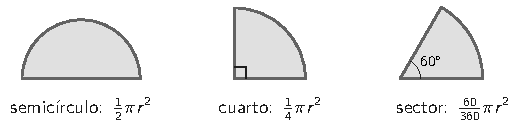
\includegraphics[width=0.5\linewidth]{geo_ci_sectores}\end{center}
\begin{ejemplo} Sector de $60°$ y radio 6: $\frac{60}{360} = \frac{1}{6}$, así que $A = \frac{1}{6} \cdot 36\pi = 6\pi$ y el arco mide $\frac{1}{6} \cdot 12\pi = 2\pi$. Semicírculo: la mitad; cuarto de círculo: la cuarta parte.\end{ejemplo}
\begin{ojo}[No olvides los lados rectos] El borde de un semicírculo es la mitad de la circunferencia \textbf{más el diámetro}: con $r = 5$, $P = 5\pi + 10$. El de un sector incluye los dos radios.\end{ojo}

\subsection{Regiones sombreadas y coronas}
\geolado[0.36]{geo_ci_sombra}{Igual que con los polígonos: área grande menos área en blanco. Un círculo que toca los cuatro lados de un cuadrado de 10 cm tiene radio 5 cm, y lo sombreado mide $100 - 25\pi \approx 21{,}5$ cm$^2$.

La \textbf{corona circular} es el anillo entre dos circunferencias de igual centro y radios $R$ y $r$: \[A = \pi R^2 - \pi r^2 = \pi(R^2 - r^2).\]}
\begin{ojo}[Corona: resta áreas, no radios] Con $R = 5$ y $r = 3$: $\pi(25 - 9) = 16\pi$. En cambio, $\pi(5 - 3)^2 = 4\pi$ está mal.\end{ojo}
\gatotip[\gatonegro]{Cuatro cuartos de círculo iguales forman un círculo completo, y dos semicircunferencias iguales, una circunferencia. ¡Junta los pedazos antes de calcular!}

\begin{elejemplo}{Tipo PAES}
\geolado[0.22]{geo_ci_ej}{En cada esquina de un cuadrado de 8 cm de lado se dibujó un cuarto de círculo con centro en el vértice y radio 4 cm, como se muestra en la figura.

¿Cuál es el área de la región sombreada?}
\alts{$(64 - 4\pi)$ cm$^2$}{$16\pi$ cm$^2$}{$(64 - 16\pi)$ cm$^2$}{$(64 - 8\pi)$ cm$^2$}
\solucion{Lo sombreado es el cuadrado menos los cuatro cuartos de círculo. El cuadrado mide $8 \cdot 8 = 64$ cm$^2$. Los cuatro cuartos, del mismo radio, forman un círculo completo de radio 4: $\pi \cdot 4^2 = 16\pi$ cm$^2$. Queda $(64 - 16\pi)$ cm$^2$.

\textit{Comprobación}: con $\pi \approx 3{,}14$, $16\pi \approx 50{,}24$ y lo sombreado mide unos 13,8 cm$^2$: positivo y menor que lo blanco \checkmark.

\textit{¿Por qué no las otras?} $(64 - 4\pi)$ resta un solo cuarto de círculo. $16\pi$ es la parte en blanco. $(64 - 8\pi)$ usa el perímetro de la circunferencia de radio 4 en vez de su área.}{C}
\end{elejemplo}
\motivacion{Los decimales de $\pi$ no se terminan nunca, y tus ganas tampoco. ¡Una vuelta completa más al temario!}

%% =====================================================================
\section{Área de superficie de cubos, paralelepípedos y cilindros}
\subsection{Los cuerpos y sus partes}
Un \textbf{paralelepípedo} (prisma recto de base rectangular) es una caja: 6 caras rectangulares, iguales de a pares. Un \textbf{cubo} tiene todas sus aristas iguales y sus 6 caras son cuadrados. Ambos tienen \textbf{6 caras, 12 aristas y 8 vértices}. Un \textbf{cilindro} tiene dos bases circulares iguales y una cara lateral curva, como una lata.
\begin{center}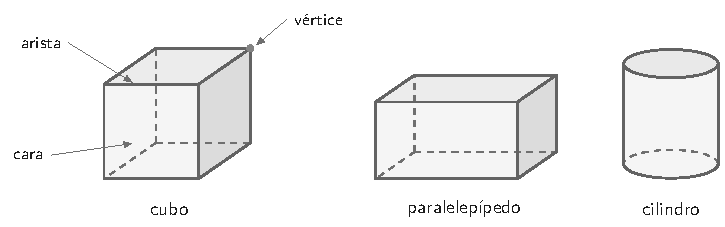
\includegraphics[width=0.62\linewidth]{geo_ac_cuerpos}\end{center}
Las líneas punteadas son aristas ocultas, que quedan detrás.

\subsection{Redes: el cuerpo desarmado}
\geolado[0.38]{geo_ac_redes}{Si desarmas una caja y la estiras sobre la mesa, obtienes su \textbf{red} o desarrollo plano. El \textbf{área de la superficie} del cuerpo es el área de su red: 6 cuadrados iguales en el cubo y 3 pares de rectángulos en el paralelepípedo.

Sirven como red de cubo la cruz y las de forma ``1--4--1''. No sirven un bloque de $2 \times 3$ ni una fila de 4 con dos cuadrados del mismo lado.}
\begin{ojo}[Truco] En una fila de 4 cuadrados, esos 4 son las paredes de alrededor; los otros dos deben ser tapa y fondo, uno a cada lado de la fila.\end{ojo}

\subsection{Área del cubo y del paralelepípedo}
\begin{clave}[Área total] Cubo de arista $a$: $6a^2$. \qquad Paralelepípedo de aristas $a$, $b$, $c$: $2(ab + bc + ac)$.\end{clave}
\begin{ejemplo} Cubo de arista 4 cm: $6 \cdot 16 = 96$ cm$^2$. Al revés, un cubo de 150 cm$^2$ tiene caras de $150 \div 6 = 25$ cm$^2$ y arista $\sqrt{25} = 5$ cm. Caja de 8, 5 y 3 cm: $2(40 + 24 + 15) = 158$ cm$^2$.\end{ejemplo}
Si el cuerpo no tiene tapa, o no se pinta la base, se resta esa cara: el cubo sin tapa tiene $5a^2$.
\begin{ojo}[No confundas con el volumen] El área total del cubo es $6a^2$ (cm$^2$); el volumen es $a^3$ (cm$^3$). Y no olvides el ``por 2'': cada tipo de cara aparece dos veces.\end{ojo}

\subsection{Área del cilindro}
\geolado[0.42]{geo_ac_red_cil}{Al abrir un cilindro, la cara lateral es un \textbf{rectángulo}: su largo es el perímetro de la base, $2\pi r$, y su ancho es la altura $h$. La etiqueta de una lata es justamente el área lateral.}
\begin{clave}[Cilindro] Lateral: $2\pi r h$ \qquad Bases: $2\pi r^2$ \qquad Total: $2\pi r h + 2\pi r^2$\end{clave}
\begin{ejemplo} Lata de radio 3 cm y altura 10 cm: lateral $60\pi$, bases $18\pi$, total $78\pi \approx 244{,}9$ cm$^2$.\end{ejemplo}
\begin{ojo}[Con diámetro] El lateral es $\pi d h$. Si pones el diámetro en lugar del radio en $2\pi r h$, el resultado sale al doble.\end{ojo}
\begin{center}\small
\begin{tabular}{lll}\toprule
Cuerpo & Área lateral & Área total\\\midrule
Cubo de arista $a$ & $4a^2$ & $6a^2$\\
Paralelepípedo $a \times b \times c$ (alto $c$) & $2(a + b)\,c$ & $2(ab + bc + ac)$\\
Cilindro de radio $r$ y altura $h$ & $2\pi r h$ & $2\pi r h + 2\pi r^2$\\\bottomrule
\end{tabular}\end{center}
\gatotip[\gatolila]{Antes de sumar, haz la lista de caras que se cuentan: ``sin tapa'', ``sin la base'', ``solo las paredes''. Y si pegas dos cuerpos, se pierden las \textbf{dos} caras que se tocan.}

\begin{elejemplo}{PAES Invierno 2026, adaptada}
\geolado[0.24]{geo_ac_mueble}{Un carpintero restaurará el siguiente mueble con forma de prisma recto de base rectangular, de 90 cm de ancho, 50 cm de fondo y 200 cm de alto.

Para la restauración, debe pintar el exterior de la estructura, sin incluir la base inferior.

¿Cuál es la medida de la superficie por pintar?}
\alts{32.500 cm$^2$}{56.000 cm$^2$}{60.500 cm$^2$}{65.000 cm$^2$}
\solucion{Calculamos el área total y le restamos la base. Frente y espalda: $2 \cdot (90 \cdot 200) = 36.000$ cm$^2$. Costados: $2 \cdot (50 \cdot 200) = 20.000$ cm$^2$. Tapa y base: $2 \cdot (90 \cdot 50) = 9000$ cm$^2$. Total: $65.000$ cm$^2$. Sin la base inferior: $65.000 - 4500 = 60.500$ cm$^2$.

\textit{Comprobación}, sumando solo lo que se pinta: $36.000 + 20.000 + 4500 = 60.500$ \checkmark.

\textit{¿Por qué no las otras?} 32.500 cm$^2$ cuenta una sola cara de cada par. 56.000 cm$^2$ quita también la tapa, que sí se pinta. 65.000 cm$^2$ incluye la base inferior.}{C}
\end{elejemplo}
\motivacion{Desarmar un cuerpo en sus caras es la clave. Ya ves las figuras por dentro y por fuera.}

%% =====================================================================
\section{Volumen de cubos, paralelepípedos y cilindros}
\subsection{¿Qué es el volumen?}
\geolado[0.28]{geo_vo_cubitos}{El \textbf{volumen} mide cuánto espacio ocupa un cuerpo: cuántos cubitos de $1 \times 1 \times 1$ caben dentro. Se mide en unidades cúbicas: cm$^3$, m$^3$.

En una caja de $4 \times 3 \times 2$ cm caben $4 \cdot 3 = 12$ cubitos en el piso y hay 2 capas: $24$ cm$^3$. Un cubo de arista $a$ tiene $V = a^3$.}
\begin{ojo}[Tres unidades distintas] Largo en cm, área en cm$^2$, volumen en cm$^3$. El volumen siempre es un producto: sumar las aristas no tiene sentido.\end{ojo}

\subsection{Paralelepípedo y cilindro}
\begin{clave}[Volumen = área de la base $\times$ altura] Cubo: $a^3$ \qquad Paralelepípedo: $a \cdot b \cdot c$ \qquad Cilindro: $\pi r^2 h$\end{clave}
\begin{ejemplo} Caja de 20, 5 y 30 cm: $3000$ cm$^3$; si se hace un 10~\% más alta, la altura pasa a 33 cm y el volumen a $3300$ cm$^3$, también un 10~\% más. Lata de radio 3 cm y altura 10 cm: $V = \pi \cdot 9 \cdot 10 = 90\pi \approx 282{,}6$ cm$^3$. Al revés: con $V = 600$, largo 10 y ancho 6, la altura es $600 \div 60 = 10$.\end{ejemplo}
\begin{ojo}[Errores del cilindro] Usar el diámetro como radio (el volumen sale 4 veces más grande), escribir $2\pi r h$ (área lateral) u olvidar elevar el radio al cuadrado. Si el cilindro está acostado, su ``altura'' es el largo.\end{ojo}

\subsection{Capacidad: litros y metros cúbicos}
La \textbf{capacidad} es el volumen que cabe dentro de un recipiente. Un cubo de 10 cm de arista contiene exactamente 1 litro.
\begin{center}\small
\begin{tabular}{ll}\toprule
Volumen & Capacidad\\\midrule
1 cm$^3$ & 1 mL\\
1 dm$^3$ $=$ 1000 cm$^3$ & 1 L\\
1 m$^3$ $=$ 1000 dm$^3$ & 1000 L\\\bottomrule
\end{tabular}\end{center}
\begin{ojo}[Tres medidas, tres veces] De m a cm se multiplica por 100, pero de m$^3$ a cm$^3$ por $100 \cdot 100 \cdot 100 = 1.000.000$. Lo más seguro es pasar las medidas a la unidad que quieras \textbf{antes} de multiplicar.\end{ojo}

\subsection{Llenado, nivel del agua y caudal}
\geolado[0.38]{geo_vo_pecera}{El agua dentro de una caja forma otra caja, con la misma base y de alto el nivel del agua.
\begin{itemize}
\item \textbf{Altura que alcanza}: 6 L $= 6000$ cm$^3$ en una pecera de base $30 \times 20$ cm suben $6000 \div 600 = 10$ cm.
\item \textbf{Objeto sumergido}: si el agua sube 2 cm, su volumen es $30 \cdot 20 \cdot 2 = 1200$ cm$^3$.
\item \textbf{Caudal}: $Q = \frac{V}{t}$. Para llenar 3000 L en 10 minutos se necesitan 300 L/min.
\end{itemize}}
\begin{ojo}[La altura del agua] Si el recipiente no está lleno, usa la altura del agua, no la del recipiente.\end{ojo}

\subsection{Cambios de escala}
\geolado[0.3]{geo_vo_escala}{Si todas las aristas se multiplican por $k$, el volumen se multiplica por $k^3$ (y el área por $k^2$): al duplicar las aristas de un cubo caben $2 \cdot 2 \cdot 2 = 8$ cubos como el original.

Si cambia una sola medida, el volumen cambia en el mismo factor. En $\pi r^2 h$ el radio cuenta doble: duplicarlo multiplica el volumen por 4; duplicar radio y altura, por 8.}
\gatotip[\gatogris]{Si un metal se funde y se rehace en piezas chicas, el volumen se conserva: divide volúmenes. Y para saber cuántas cajas caben en un contenedor, cuenta cuántas entran a lo largo de cada medida y multiplica.}

\begin{elejemplo}{PAES Invierno 2027, adaptada}
\geolado[0.26]{geo_vo_estanque}{Un estanque de agua tiene forma de prisma recto de base rectangular, cuya base mide 4 m de largo y 3 m de ancho. Se debe llenar hasta 2 m de altura con agua proveniente de un ducto.

Para calcular el caudal del agua que sale de un ducto se puede usar la expresión $\frac{V}{t}$, donde $V$ es el volumen de agua que sale del ducto durante $t$ unidades de tiempo.}
¿Cuál de las siguientes expresiones corresponde al caudal de agua, en $\frac{\text{m}^3}{\text{h}}$, que debe salir del ducto para que el estanque se llene hasta 2 m de altura en 10 horas?
\alts{$\dfrac{4 \cdot 3 \cdot 2}{10}$}{$\dfrac{4 + 3 + 2}{10}$}{$\dfrac{2(4 + 3)}{10}$}{$\dfrac{2(4 \cdot 3 + 2 \cdot 4 + 2 \cdot 3)}{10}$}
\solucion{El agua forma una caja de $4 \times 3$ m de base y 2 m de alto: $V = 4 \cdot 3 \cdot 2 = 24$ m$^3$. En $t = 10$ horas, el caudal es $\dfrac{V}{t} = \dfrac{4 \cdot 3 \cdot 2}{10}$, o sea 2,4 m$^3$ por hora.

\textit{Comprobación}: en 10 horas salen $2{,}4 \cdot 10 = 24$ m$^3$ \checkmark.

\textit{¿Por qué no las otras?} $\frac{4 + 3 + 2}{10}$ suma las medidas en vez de multiplicarlas. $\frac{2(4 + 3)}{10}$ usa el perímetro de la base por la altura, que es parte del área lateral. La última usa el área total de la caja: mide superficie, no volumen.}{A}
\end{elejemplo}
\motivacion{Llenaste otro tema hasta el borde. Tu capacidad para aprender es mucho más grande que cualquier cilindro.}

%% =====================================================================
\section{Puntos y vectores en el plano}
\subsection{El plano cartesiano y los cuadrantes}
\geolado[0.34]{tra_plano_cuadrantes}{El \textbf{plano cartesiano} tiene dos rectas numéricas perpendiculares, el \textbf{eje X} (horizontal) y el \textbf{eje Y} (vertical), que se cortan en el \textbf{origen} $O = (0, 0)$. Cada punto es un \textbf{par ordenado} $(x, y)$: primero cuánto avanzas en horizontal, después cuánto subes o bajas. $C(-2, -3)$ está 2 a la izquierda y 3 hacia abajo.

\begin{center}\small
\begin{tabular}{ccc}\toprule
Cuadrante & $x$ & $y$\\\midrule
I (arriba, derecha) & $+$ & $+$\\
II (arriba, izquierda) & $-$ & $+$\\
III (abajo, izquierda) & $-$ & $-$\\
IV (abajo, derecha) & $+$ & $-$\\\bottomrule
\end{tabular}\end{center}}

\subsection{Leer coordenadas sin equivocarse}
\textbf{El orden importa}: $(2, 5)$ y $(5, 2)$ son puntos distintos. Un punto sobre el eje X tiene $y = 0$, como $(4, 0)$; uno sobre el eje Y tiene $x = 0$, como $(0, -3)$. Los puntos de los ejes no son de ningún cuadrante.
\begin{ejemplo} Si $P(a, b)$ está en el cuadrante II, entonces $a < 0$ y $b > 0$. El punto $Q(b, a)$ tiene primera coordenada positiva y segunda negativa: está en el cuadrante IV.\end{ejemplo}
\begin{ojo}[Primero la $x$] En $(x, y)$ siempre va primero lo horizontal, como en el abecedario. Y si la cuadrícula tiene escala, multiplica los cuadros por lo que vale cada uno.\end{ojo}

\subsection{¿Qué es un vector?}
Un \textbf{vector} $\vec{u} = (a, b)$ es una flecha que indica un \textbf{desplazamiento}: $(3, 2)$ es 3 a la derecha y 2 hacia arriba. Tiene \textbf{magnitud} (su largo), \textbf{dirección} (su inclinación) y \textbf{sentido} (hacia cuál lado apunta). Flechas iguales dibujadas en distintos lugares son el mismo vector.
\begin{clave}[Vector opuesto] El opuesto de $(a, b)$ es $(-a, -b)$: misma magnitud y dirección, sentido contrario.\end{clave}

\subsection{El vector entre dos puntos: final menos inicial}
\begin{clave}[Vector de $A$ a $B$] $\overrightarrow{AB} = B - A$ (final menos inicial) \qquad Magnitud de $(a, b)$: $\sqrt{a^2 + b^2}$\end{clave}
\geolado[0.27]{tra_vector_ab}{Con $A(1, 2)$ y $B(5, -1)$: $\overrightarrow{AB} = (5 - 1, -1 - 2) = (4, -3)$: 4 a la derecha y 3 hacia abajo. Su magnitud es $\sqrt{16 + 9} = 5$.


\textit{Comprobación}: $A + (4, -3) = (5, -1) = B$ \checkmark.}
\begin{ojo}[Al revés cambia el signo] $\overrightarrow{BA} = A - B = (-4, 3)$, el opuesto de $\overrightarrow{AB}$. Y la magnitud no es la suma: $|(6, 8)| = \sqrt{100} = 10$, no 14.\end{ojo}

\subsection{Sumar vectores y multiplicarlos por un número}
\geolado[0.27]{tra_suma_vectores}{Se opera coordenada con coordenada: $(a, b) + (c, d) = (a + c, b + d)$ y $k(a, b) = (ka, kb)$.

Con $\vec{u} = (4, 1)$ y $\vec{v} = (1, 3)$: $\vec{u} + \vec{v} = (5, 4)$, $\vec{u} - \vec{v} = (3, -2)$ y $2\vec{u} = (8, 2)$. En el dibujo, la suma es hacer un desplazamiento y después el otro. Multiplicar por un número negativo da vuelta el sentido.}
\begin{ojo}[No se multiplican coordenadas] $(4, 1) + (1, 3)$ no es $(4 \cdot 1, 1 \cdot 3)$.\end{ojo}

\subsection{Trasladar un punto con un vector}
\begin{clave}[Traslación de un punto] $P' = P + \vec{v}$ \qquad y al revés \qquad $P = P' - \vec{v}$\end{clave}
\begin{ejemplo} $P(-3, 4)$ y $\vec{v} = (5, -6)$: $P' = (-3 + 5, 4 - 6) = (2, -2)$. Si $P'(1, 1)$ y $\vec{v} = (4, -2)$, entonces $P = (1 - 4, 1 - (-2)) = (-3, 3)$.\end{ejemplo}
\textbf{Dos traslaciones seguidas} equivalen a una sola con la suma de los vectores: $(2, 1)$ y luego $(3, -4)$ es lo mismo que $(5, -3)$. Con el norte hacia arriba, el este es $x$ positivo, el oeste $x$ negativo, el norte $y$ positivo y el sur $y$ negativo: ``3 km al oeste y 2 km al norte'' es $(-3, 2)$.
\gatotip[\gatonaranjo]{Comprueba siempre: el punto original más el vector debe darte la imagen. Y restar un negativo es sumar: $1 - (-2) = 3$.}
\gatotip[\gatoatigrado]{En un paralelogramo $ABCD$, el vector de $A$ a $D$ es igual al de $B$ a $C$: $D = A + (C - B)$.}

\begin{elejemplo}{PAES Invierno 2026, adaptada}
Un barco que inicia un recorrido realiza los siguientes movimientos, en este orden: 4 kilómetros al oeste, 6 kilómetros al norte, 7 kilómetros al este, 9 kilómetros al sur y 5 kilómetros al oeste.

¿Cuál es la ubicación final del barco con respecto a su ubicación inicial?
\alts{2 kilómetros al este y 3 kilómetros al norte}{16 kilómetros al oeste y 15 kilómetros al sur}{2 kilómetros al oeste y 3 kilómetros al sur}{3 kilómetros al oeste y 2 kilómetros al sur}
\solucion{Cada movimiento es un vector, con este y norte positivos: $(-4, 0)$, $(0, 6)$, $(7, 0)$, $(0, -9)$ y $(-5, 0)$. El desplazamiento total es la suma. Horizontal: $-4 + 7 - 5 = -2$, o sea 2 km al oeste. Vertical: $6 - 9 = -3$, o sea 3 km al sur. El barco termina en $(-2, -3)$: 2 km al oeste y 3 km al sur.
\begin{center}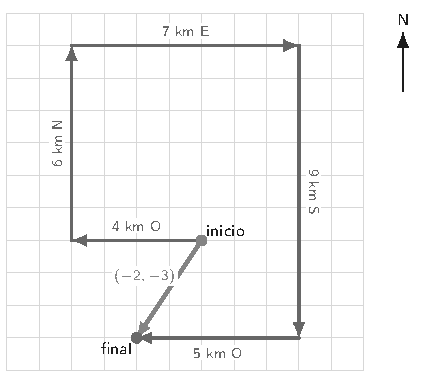
\includegraphics[width=0.3\linewidth]{tra_barco}\end{center}
\textit{Comprobación}: en la cuadrícula, la flecha que une el inicio con el final avanza 2 cuadros a la izquierda y baja 3 \checkmark.

\textit{¿Por qué no las otras?} ``2 al este y 3 al norte'' tiene los sentidos al revés. ``16 al oeste y 15 al sur'' suma todos los kilómetros sin fijarse en el sentido. ``3 al oeste y 2 al sur'' intercambia lo horizontal con lo vertical.}{C}
\end{elejemplo}
\motivacion{Ya te mueves en el plano con coordenadas y vectores. Tu vector apunta directo a la meta.}

%% =====================================================================
\section{Traslación y reflexión}
\subsection{Transformaciones isométricas}
Una \textbf{transformación isométrica} mueve una figura sin deformarla: la imagen tiene la misma forma y el mismo tamaño. Hay tres: \textbf{traslación} (desliza según un vector), \textbf{reflexión} (refleja como un espejo respecto de una recta o de un punto) y \textbf{rotación} (gira en torno a un punto). La imagen del punto $A$ se escribe $A'$.
\begin{center}\small
\begin{tabular}{lccc}\toprule
¿Se conserva? & Traslación & Reflexión & Rotación\\\midrule
Lados, ángulos, perímetro y área & sí & sí & sí\\
Orientación (sentido de recorrido de los vértices) & sí & \textbf{no}, se invierte & sí\\\bottomrule
\end{tabular}\end{center}

\subsection{Traslación de una figura}
\begin{clave}[Traslación según $(a, b)$] $(x, y) \to (x + a, y + b)$\end{clave}
\geolado[0.36]{tra_tras_triangulo}{Se traslada \textbf{cada vértice} con el mismo vector y se unen las imágenes.

Con $A(-5, 1)$, $B(-2, 1)$, $C(-4, 4)$ y $\vec{v} = (6, -3)$: $A'(1, -2)$, $B'(4, -2)$ y $C'(2, 1)$. La figura no gira ni se da vuelta. Si conoces un vértice y su imagen, el vector es imagen menos original.}

\subsection{Reflexión respecto de los ejes}
\geolado[0.3]{tra_refl_ejes}{En una reflexión, cada punto y su imagen quedan a la misma distancia del eje, uno a cada lado, en una línea perpendicular al eje.

\textbf{Respecto del eje X} la $x$ queda igual y la $y$ cambia de signo: $(x, y) \to (x, -y)$; $(3, 5) \to (3, -5)$.

\textbf{Respecto del eje Y} la $y$ queda igual y la $x$ cambia de signo: $(x, y) \to (-x, y)$; $(3, 5) \to (-3, 5)$.

La letra F de la figura queda ``al revés'', como en un espejo.}
\begin{ojo}[Para no confundirte] Cambia la coordenada que \textbf{no} lleva el nombre del eje. Reflejar respecto del eje X manda la figura hacia abajo.\end{ojo}

\subsection{\texorpdfstring{Reflexión respecto de las rectas $x = a$ e $y = b$}{Reflexión respecto de las rectas x = a e y = b}}
\geolado[0.34]{tra_refl_recta}{Cuenta la distancia del punto a la recta y pasa la misma distancia al otro lado. $B(1, 1)$ respecto de $x = 3$: de 1 a 3 hay 2 unidades; $3 + 2 = 5$ y la altura no cambia, $B' = (5, 1)$.}
\begin{clave}[Fórmulas] Respecto de $x = a$: $(x, y) \to (2a - x,\ y)$. \qquad Respecto de $y = b$: $(x, y) \to (x,\ 2b - y)$.\end{clave}
El eje queda justo \textbf{al medio} entre un punto y su imagen: el promedio de 1 y 5 es 3. Así se encuentra el eje si te dan un punto y su imagen.

\subsection{\texorpdfstring{Reflexión respecto de $y = x$ y respecto del origen}{Reflexión respecto de y = x y respecto del origen}}
\geolado[0.32]{tra_refl_yx}{\textbf{Respecto de la recta $y = x$} las coordenadas se intercambian: $(4, 1) \to (1, 4)$ y $(-2, 3) \to (3, -2)$.

\textbf{Respecto del origen} las dos coordenadas cambian de signo: $(4, 1) \to (-4, -1)$. Es lo mismo que reflejar respecto del eje X y luego del eje Y, y que girar $180^\circ$ en torno al origen.}
\begin{center}\small
\begin{tabular}{cccccc}\toprule
eje X & eje Y & recta $x = a$ & recta $y = b$ & recta $y = x$ & origen\\\midrule
$(x, -y)$ & $(-x, y)$ & $(2a - x, y)$ & $(x, 2b - y)$ & $(y, x)$ & $(-x, -y)$\\\bottomrule
\end{tabular}\end{center}
\begin{ojo}[Con $y = x$ no cambian los signos] Solo se intercambian: $(4, -1) \to (-1, 4)$.\end{ojo}

\subsection{Dos transformaciones seguidas}
Se hace la primera y a su resultado se le aplica la segunda. \textbf{El orden importa}.
\begin{ejemplo} $P(2, 3)$: reflexión respecto del eje X, $(2, -3)$, y luego traslación según $(1, 4)$, $(3, 1)$. En el otro orden da $(3, -7)$. Si la regla es $(x + 1, 4 - y)$, eso es reflejar respecto del eje X y trasladar según $(1, 4)$: la imagen de $(5, -2)$ es $(6, 6)$.\end{ejemplo}
\begin{clave}[Dos reflexiones] Respecto del mismo eje dos veces: el punto vuelve. Respecto de dos rectas paralelas: una traslación del doble de la distancia entre ellas. Respecto del eje X y luego del eje Y: la reflexión respecto del origen.\end{clave}
\gatotip[\gatoblanco]{Doblar papel es reflejar: si perforas una hoja doblada, al abrirla la perforación aparece reflejada respecto de la línea del doblez. Para deshacer dos transformaciones, deshazlas en orden inverso.}

\begin{elejemplo}{PAES Invierno 2026, adaptada}
A una figura se le aplica una reflexión y luego una traslación. La imagen del vértice $(x, y)$ es $(x - 3, 4 - y)$. A otra figura se le aplican las mismas transformaciones isométricas y en el mismo orden.

Si $(-2, -5)$ es un vértice de esta figura, ¿cuáles son las coordenadas de la imagen de este vértice?
\alts{$(-5, -1)$}{$(5, 9)$}{$(-5, 9)$}{$(-5, -9)$}
\solucion{Basta reemplazar $x = -2$ e $y = -5$ en la regla: $x - 3 = -2 - 3 = -5$ y $4 - y = 4 - (-5) = 9$. La imagen es $(-5, 9)$.

\textit{Comprobación} por pasos: la regla es una reflexión respecto del eje X seguida de una traslación según $(-3, 4)$; $(-2, -5) \to (-2, 5) \to (-5, 9)$ \checkmark.

\textit{¿Por qué no las otras?} $(-5, -1)$ calcula $4 + y$. $(5, 9)$ cambia el signo de la $x$. $(-5, -9)$ se equivoca con el menos: escribe $4 - (-5)$ como $-(4 + 5)$.}{C}
\end{elejemplo}
\motivacion{Trasladar y reflejar no cambian la figura, solo su lugar. Tú sí estás cambiando: cada tema te hace más fuerte.}

%% =====================================================================
\section{Rotación}
\subsection{¿Qué es una rotación?}
Una \textbf{rotación} gira una figura en torno a un punto fijo, el \textbf{centro de rotación}. Se describe con tres datos: el \textbf{centro} (casi siempre el origen), el \textbf{ángulo} (en la PAES, $90^\circ$, $180^\circ$ o $270^\circ$) y el \textbf{sentido}: \textbf{horario}, como los punteros del reloj, o \textbf{antihorario}, al revés. Cada punto se mantiene a la misma distancia del centro, así que la figura no cambia de tamaño ni se da vuelta.

\subsection{Las reglas de 90°, 180° y 270°}
\geolado[0.34]{tra_rot_tabla}{\begin{center}\small
\begin{tabular}{lcc}\toprule
Rotación en torno al origen & Regla & $P(4, 2)$\\\midrule
$90^\circ$ antihorario & $(-y, x)$ & $(-2, 4)$\\
$180^\circ$ (cualquier sentido) & $(-x, -y)$ & $(-4, -2)$\\
$270^\circ$ antihorario $= 90^\circ$ horario & $(y, -x)$ & $(2, -4)$\\
$360^\circ$ & $(x, y)$ & $(4, 2)$\\\bottomrule
\end{tabular}\end{center}
$270^\circ$ en un sentido es lo mismo que $90^\circ$ en el otro. $180^\circ$ da igual en un sentido o en el otro, y equivale a la reflexión respecto del centro.}
\begin{ejemplo} $90^\circ$ horario a $P(-2, 5)$: $(y, -x) = (5, 2)$. $90^\circ$ antihorario a $(4, -1)$: $(-y, x) = (1, 4)$, porque $-(-1) = 1$.\end{ejemplo}

\subsection{Trucos para no girar al revés}
\begin{clave}[Los cuadrantes] Con $90^\circ$ antihorario, cada punto avanza un cuadrante: I $\to$ II $\to$ III $\to$ IV $\to$ I. Con $90^\circ$ horario retrocede uno. Con $180^\circ$ va al cuadrante opuesto.\end{clave}
También sirve girar la hoja un cuarto de vuelta, o probar con $(1, 0)$: con $90^\circ$ antihorario debe quedar arriba, en $(0, 1)$. Varias rotaciones con el mismo centro se suman: tres de $90^\circ$ antihorario son $270^\circ$, o sea $90^\circ$ horario; cuatro devuelven la figura. Para deshacer una rotación, gira el mismo ángulo en sentido contrario.
\gatotip[\gatolila]{Los punteros del reloj giran en sentido horario, y el minutero avanza $360^\circ \div 60 = 6^\circ$ por minuto: en 20 minutos gira $120^\circ$.}

\subsection{Rotar en torno a otro punto}
\begin{clave}[Centro $C$] Mira el punto desde el centro, gíralo y vuelve: 1. resta el centro, $P - C$; 2. aplica la regla; 3. suma el centro.\end{clave}
\geolado[0.27]{tra_rot_centro}{$P(5, 2)$ en $90^\circ$ antihorario en torno a $C(2, 1)$: $P - C = (3, 1) \to (-1, 3)$, y sumando $C$, $P' = (1, 4)$.}
\begin{ojo}[No olvides volver] Quedarse con $(-1, 3)$ es el error más común: esa es la posición respecto de $C$. Con $180^\circ$, el centro es el punto medio entre el punto y su imagen: $P' = 2C - P$.\end{ojo}

\subsection{¿Qué transformación es?}
\geolado[0.28]{tra_rot_identificar}{Para reconocer qué transformación lleva una figura a otra:

\textbf{1. ¿Está dada vuelta?} Si se ve como en un espejo, es una \textbf{reflexión}.

\textbf{2. Si no, ¿está girada?} Si apunta en otra dirección, es una \textbf{rotación}; si apunta igual y solo cambió de lugar, es una \textbf{traslación}.

Después confirma aplicando la regla a un vértice. La F girada en $180^\circ$ queda cabeza abajo, pero se puede leer girando la hoja; la reflejada no.}
\gatotip[\gatonegro]{Para seguir una flecha, usa ángulos: este $0^\circ$, noreste $45^\circ$, norte $90^\circ$, sur $270^\circ$. Rotar en sentido antihorario suma grados, y una traslación nunca cambia hacia dónde apunta.}

\begin{elejemplo}{PAES Invierno 2027, adaptada}
\geolado[0.32]{tra_rot_proteina}{En el gráfico se representa una simulación bidimensional de una proteína con su grupo metilo, localizado en el punto $P(5, 3)$, con el objetivo de estudiar su desplazamiento. Dicha proteína con su grupo metilo es sometida a una rotación de $90^\circ$ en sentido antihorario con respecto al origen del sistema de coordenadas cartesianas.

¿Cuáles son las coordenadas del grupo metilo después de la rotación?}
\alts{$(3, -5)$}{$(-3, 5)$}{$(-5, -3)$}{$(5, -3)$}
\solucion{La regla de $90^\circ$ antihorario en torno al origen es $(x, y) \to (-y, x)$. Con $x = 5$ e $y = 3$ queda $(-3, 5)$.

\textit{Comprobación}: $P$ estaba en el cuadrante I y la imagen está en el II, como corresponde; además la distancia al origen se mantiene, $\sqrt{25 + 9} = \sqrt{9 + 25} = \sqrt{34}$ \checkmark.

\textit{¿Por qué no las otras?} $(3, -5)$ gira $90^\circ$ en sentido horario. $(-5, -3)$ gira $180^\circ$. $(5, -3)$ refleja respecto del eje X.}{B}
\end{elejemplo}
\motivacion{Girar en 90 o 180 grados ya no es un misterio. Y si algo sale mal, das la vuelta y lo intentas otra vez.}

%% =====================================================================
\section{Semejanza y escalas}
\subsection{Figuras semejantes}
Dos figuras son \textbf{semejantes} ($\sim$) si tienen la misma forma, aunque distinto tamaño: una es ampliación o reducción de la otra. Sus \textbf{ángulos} correspondientes son iguales y sus \textbf{lados} son \textbf{proporcionales}: todos se multiplican por el mismo número $k$, la \textbf{razón de semejanza}.
\begin{center}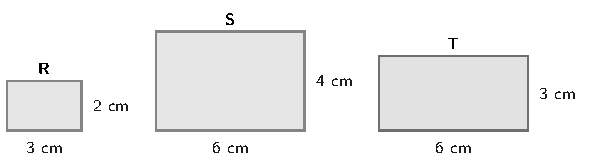
\includegraphics[width=0.52\linewidth]{sem_rectangulos}\end{center}
\begin{ejemplo} $R$ mide $3 \times 2$ y $S$ mide $6 \times 4$: $\frac{6}{3} = \frac{4}{2} = 2$, son semejantes con $k = 2$. $T$ mide $6 \times 3$: $\frac{6}{3} = 2$, pero $\frac{3}{2} = 1{,}5$; no es semejante a $R$.\end{ejemplo}
\begin{ojo}[Proporcional no es sumar lo mismo] Sumarle 3 a cada lado de $3 \times 2$ da $6 \times 5$, que no es semejante. En la semejanza se \textbf{multiplica}.\end{ojo}

\subsection{Lados homólogos y razón de semejanza}
Los \textbf{lados homólogos} son los que se corresponden. Si $\triangle ABC \sim \triangle DEF$, el orden de las letras lo dice: $AB$ con $DE$, $BC$ con $EF$ y $AC$ con $DF$.
\begin{ejemplo} $\triangle ABC \sim \triangle DEF$ con $AB = 3$, $BC = 4$, $AC = 5$, $DE = 6$ y $DF = 10$. La razón es $k = \frac{DE}{AB} = 2$ (y $\frac{DF}{AC} = 2$ lo confirma), así que $EF = 2 \cdot 4 = 8$. Con proporción: $\frac{x}{4} = \frac{6}{3}$, $3x = 24$, $x = 8$.\end{ejemplo}

\subsection{Triángulos semejantes: basta con dos ángulos}
\geolado[0.3]{sem_encajados}{Dos triángulos con \textbf{dos ángulos iguales} son semejantes (criterio AA); el tercero también es igual, porque suman $180^\circ$. También lo son si sus tres lados son proporcionales (LLL) o si dos lados son proporcionales y el ángulo entre ellos es igual (LAL).

Si en $ABC$ se traza $DE$ paralelo a $BC$, el triángulo $ADE$ es semejante a $ABC$. Con $AD = 2$, $DB = 4$ y $DE = 3$: $AB = 6$, $k = \frac{6}{2} = 3$ y $BC = 3 \cdot 3 = 9$.}
\begin{ojo}[El error clásico] El homólogo de $AB$ (lado completo del grande) es $AD$ (lado completo del chico), no el pedazo $DB$.\end{ojo}

\subsection{Sombras, postes y alturas}
\geolado[0.4]{sem_sombras}{A la misma hora, los rayos del sol llegan paralelos: cada objeto vertical, su sombra y el rayo forman triángulos rectángulos semejantes. La razón altura\,:\,sombra es la misma para todos.

Un poste de 4 m da 6 m de sombra. Una persona de 1,6 m da $\frac{1{,}6}{x} = \frac{4}{6}$, o sea $4x = 9{,}6$ y $x = 2{,}4$ m.}
\begin{ojo}[Ordena antes de calcular] Alturas arriba y sombras abajo en las dos fracciones; si mezclas, el resultado sale al revés.\end{ojo}
\gatotip[\gatogris]{Espejos en el suelo, rampas con soportes y ríos que no se pueden cruzar esconden lo mismo: dos triángulos semejantes. Empareja los lados homólogos y escribe la misma razón en ambos.}

\subsection{Planos, mapas y maquetas a escala}
Una \textbf{escala $1 : n$} significa que 1 cm del dibujo representa $n$ cm de la realidad. Del dibujo a la realidad se multiplica por $n$; de la realidad al dibujo se divide.
\begin{ejemplo} Mapa 1\,:\,50.000 con 6 cm entre dos pueblos: $6 \cdot 50.000 = 300.000$ cm $= 3000$ m $= 3$ km. Edificio de 45 m en maqueta 1\,:\,300: $\frac{4500}{300} = 15$ cm. Si 2 cm del mapa son 200 m $= 20.000$ cm, 1 cm son 10.000 cm: escala 1\,:\,10.000.\end{ejemplo}
\begin{ojo}[Mismas unidades] La escala compara centímetros con centímetros: 1 m $= 100$ cm, 1 km $= 100.000$ cm y 1 m$^2$ $= 10.000$ cm$^2$. En una escala gráfica, como ``2 cm $=$ 1 km'', cuenta cuántas veces cabe la barra.\end{ojo}

\subsection{\texorpdfstring{Perímetro por $k$, área por $k^2$}{Perímetro por k, área por k al cuadrado}}
\geolado[0.3]{sem_areas}{Si una figura se amplía con razón $k$, cada \textbf{longitud} (lados, perímetro, alturas) se multiplica por $k$ y el \textbf{área} por $k^2$: al duplicar el lado de un cuadrado caben $2 \cdot 2 = 4$ cuadrados como el original.}
\begin{ejemplo} Triángulo de perímetro 10 cm y área 4 cm$^2$, ampliado con $k = 3$: perímetro 30 cm y área $4 \cdot 9 = 36$ cm$^2$. Al revés: si las áreas de dos cuadrados son 9 y 36, $k^2 = 4$ y $k = 2$. En un plano 1\,:\,100 las áreas se multiplican por $100^2 = 10.000$.\end{ejemplo}
\gatotip[\gatoatigrado]{En un plano a escala, lo más seguro es pasar primero cada lado a la realidad y después calcular el área. Y revisa al final: lo grande debe quedar grande y lo chico, chico.}

\begin{elejemplo}{PAES Invierno 2027, adaptada}
\geolado[0.3]{sem_mapa_ruta}{Martina debe ir de su casa al colegio y para esto revisa un mapa. En la figura se presenta el mapa y la medida, en el mapa, del recorrido que debe hacer. Se sabe que 3 cm en el mapa equivalen a 150 m de distancia en la realidad.

¿Cuál es la distancia real que debe recorrer Martina?}
\alts{450 m}{650 m}{1950 m}{50 m}
\solucion{Si 3 cm son 150 m, entonces 1 cm del mapa es $\frac{150}{3} = 50$ m. El recorrido mide 13 cm en el mapa: $13 \cdot 50 = 650$ m.

\textit{Comprobación} con una proporción: $\frac{3}{150} = \frac{13}{x}$, así que $3x = 1950$ y $x = 650$ \checkmark.

\textit{¿Por qué no las otras?} 450 m multiplica 150 m por 3. 1950 m supone que cada centímetro vale 150 m. 50 m es lo que vale un solo centímetro.}{B}
\end{elejemplo}
\motivacion{Misma forma, distinto tamaño: en el mapa tus metas se ven chicas, pero a escala real son enormes. Cerraste Geometría: ¡bravo!}


\chapter{Probabilidad y Estadística}
%% Diagrama de cajón horizontal: \pyecaja{y}{mín}{Q1}{Me}{Q3}{máx}, dentro de un tikzpicture con la escala en x.
\newcommand{\pyecaja}[6]{%
  \draw[thick,gris] (#2,#1) -- (#3,#1) (#5,#1) -- (#6,#1);
  \draw[thick,gris] (#2,#1-0.18) -- (#2,#1+0.18) (#6,#1-0.18) -- (#6,#1+0.18);
  \draw[thick,nar,fill=narc!35] (#3,#1-0.32) rectangle (#5,#1+0.32);
  \draw[very thick,nard] (#4,#1-0.32) -- (#4,#1+0.32);}

%% =====================================================================
\section{Tablas de frecuencia}

\subsection{Para qué sirve una tabla}
Cuando hay muchos datos, la tabla los resume: en una columna van los valores o categorías $x_i$ y en la otra, cuántas veces aparece cada uno. Esa cantidad es la \textbf{frecuencia absoluta} $f_i$ (la PAES le dice ``cantidad'' o ``frecuencia'').

\begin{clave}[El total] $n = \sum f_i$: el total de datos se obtiene sumando la columna de frecuencias, nunca la de valores.\end{clave}

\begin{ejemplo}
Puntajes de una prueba en un curso:\par\smallskip
\centering\begin{tabular}{@{}l*{7}{c}c@{}}\toprule
Puntaje $x_i$ & 1 & 2 & 3 & 4 & 5 & 6 & 7 & Total\\\midrule
Frecuencia $f_i$ & 2 & 4 & 4 & 5 & 7 & 3 & 5 & $n = 30$\\\bottomrule
\end{tabular}\par\smallskip
\raggedright El curso tiene $2+4+4+5+7+3+5 = 30$ estudiantes; 7 es solo la cantidad de filas.
\end{ejemplo}

\subsection{Frecuencia relativa}
La \textbf{frecuencia relativa} dice qué parte del total representa cada fila. Las $h_i$ siempre suman $1$ (o $100\%$).
\begin{clave}[Relativa] \[ h_i = \frac{f_i}{n} \qquad h_i\% = \frac{f_i}{n}\cdot 100\% \qquad\text{y al revés}\qquad f_i = h_i\cdot n \]\end{clave}

\begin{minipage}[t]{0.42\linewidth}\vspace{0pt}\centering\small
\begin{tabular}{@{}ccc@{}}\toprule
Mascotas & $f_i$ & $h_i$\\\midrule
0 & 12 & $0{,}24$\\ 1 & 10 & $0{,}20$\\ 2 & 15 & $0{,}30$\\ 3 & 6 & $0{,}12$\\ 4 & 5 & $0{,}10$\\ 5 o más & 2 & $0{,}04$\\\midrule
Total & $n = 50$ & $1$\\\bottomrule
\end{tabular}
\end{minipage}\hfill
\begin{minipage}[t]{0.54\linewidth}\vspace{0pt}
\begin{ojo}[La PAES pide la expresión] Casi siempre las alternativas son del tipo $\frac{13}{50}\cdot 100\%$. Reconoce el numerador (los casos que cumplen) y el denominador ($n$): suelen poner uno bien y el otro mal.\end{ojo}
\begin{ojo}[Grupos de distinto tamaño] Para comparar niveles con distinta cantidad de alumnos se comparan porcentajes, cada uno sobre su propio total: $\frac{20}{80} = 25\%$ es mayor que $\frac{25}{125} = 20\%$, aunque 25 sea más que 20.\end{ojo}
\end{minipage}

\subsection{Frecuencias acumuladas}
La \textbf{acumulada} $F_i = f_1 + \dots + f_i$ suma desde la primera fila hasta la fila $i$, y $H_i = F_i/n$ es la relativa acumulada. Como crece fila a fila, $f_i = F_i - F_{i-1}$: si $F_3 = 20$ y $F_2 = 14$, entonces $f_3 = 6$.

\begin{clave}[Traducción]
``A lo más 2'' o ``no supera 2'' $=$ 2 o menos: se acumula hasta la fila del 2.\\
``Al menos 3'' o ``como mínimo 3'' $=$ 3 o más: se suman las filas desde el 3, o bien $n - F_2$.\\
``Más de 3'' $=$ 4 o más (el 3 no entra). ``Menos de 3'' $=$ 0, 1 o 2.
\end{clave}

\begin{ejemplo} Con la tabla de mascotas: familias con 3 o más son $6+5+2 = 13$, es decir $\frac{13}{50}\cdot 100\% = 26\%$. Con a lo más 2 son $12+10+15 = 37 = F_3$ y $H_3 = 0{,}74$.\end{ejemplo}

\subsection{Categorías abiertas e intervalos}
Filas como ``5 o más'' o ``18--24 años'' dicen cuántos datos hay, pero no su valor exacto. Cuando el límite pedido cae \textbf{dentro} de un intervalo, la respuesta depende de si piden la mayor o la menor cantidad posible.

\begin{ojo}[Máximo y mínimo] ¿Cuántos trabajadores, como máximo, tienen a lo más 40 años? La fila 35--44 contiene el 40: para el \textbf{máximo} cuenta entera; para el \textbf{mínimo} aporta 0.\end{ojo}

\gatotip[\gatonaranjo]{Antes de sumar, marca con el lápiz las filas que cumplen la condición. ``Como mínimo 6'' incluye al 6: es el descuido que más puntos regala.}

\begin{elejemplo}{PAES Invierno 2027, adaptada}
En la siguiente tabla se presenta el tiempo que las personas han trabajado en un colegio.
\begin{center}\small
\begin{tabular}{@{}l*{10}{c}@{}}\toprule
Tiempo de trabajo en años & 1 & 2 & 3 & 4 & 5 & 6 & 7 & 8 & 9 & 10\\\midrule
Cantidad de personas & 2 & 4 & 5 & 4 & 2 & 6 & 2 & 5 & 3 & 2\\\bottomrule
\end{tabular}
\end{center}
El colegio entregará un bono a quienes hayan trabajado \textbf{como mínimo 6 años}. ¿Cuántas personas recibirán el bono?
\alts{12}{17}{18}{23}
\solucion{``Como mínimo 6 años'' significa 6 o más: se suman las filas 6, 7, 8, 9 y 10, es decir $6+2+5+3+2 = 18$ personas. Los distractores: 12 es sumar desde 7 (dejar fuera el 6); 17 es sumar de 1 a 5 (los que \textbf{no} reciben bono); 23 es sumar desde 5.}{C}
\end{elejemplo}

%% =====================================================================
\section{Gráficos}

\subsection{Cada gráfico cuenta algo distinto}
El gráfico de \textbf{barras} compara categorías: la altura es $f_i$ o $h_i\%$. El \textbf{circular} muestra partes de un total. El de \textbf{líneas} muestra cómo cambia algo en el tiempo. En un \textbf{pictograma} cada ícono vale una cantidad fija: 16 íconos de 4 personas son 64 personas.

\begin{clave}[Para elegir gráfico] ¿Categorías que se comparan? Barras. ¿Porcentajes que suman $100\%$? Circular. ¿Algo que cambia en el tiempo? Líneas.\end{clave}
\begin{ojo}[Mira el eje] Si el eje está en $\%$, la altura no es la cantidad: el $25\%$ de 80 alumnos son $0{,}25\cdot 80 = 20$.\end{ojo}

\begin{minipage}[c]{0.46\linewidth}\centering
\begin{tikzpicture}
\begin{axis}[ybar,width=6.4cm,height=4.4cm,ymin=0,ymax=8.5,bar width=13pt,xtick={1,...,5},xticklabels={Lun,Mar,Mié,Jue,Vie},
  axis lines*=left,ylabel={celulares},nodes near coords,every node near coord/.append style={font=\scriptsize},tick label style={font=\small},enlarge x limits=0.15,ytick={0,2,...,8}]
\addplot[fill=nar,draw=nard] coordinates {(1,3) (2,6) (3,5) (4,2) (5,7)};
\draw[dashed,azul,thick] (axis cs:0.4,5) -- (axis cs:5.6,5);
\end{axis}
\end{tikzpicture}
\end{minipage}\hfill
\begin{minipage}[c]{0.5\linewidth}
Celulares vendidos por día. Si la meta es vender \textbf{al menos 5}, se cumple el martes, el miércoles y el viernes: el 5 cuenta.
\end{minipage}

\subsection{Gráfico circular}
Cada sector es una frecuencia relativa y el círculo completo es el $100\%$. Un sector de $90^\circ$ es $\frac{90}{360} = \frac14 = 25\%$ del total.
\begin{clave}[Circular] \[ \text{ángulo}_i = h_i\cdot 360^\circ \qquad f_i = h_i\cdot n \qquad n = \frac{f_i}{h_i} \]\end{clave}
\begin{ejemplo} De 240 encuestados, el sector de $90^\circ$ son $0{,}25\cdot 240 = 60$ personas. Y al revés: si 85 artículos son el $25\%$, el total es $\frac{85}{0{,}25} = 340$.\end{ejemplo}

\subsection{Gráfico de líneas}
Interesan la tendencia, los máximos y mínimos, y las subidas y bajadas. ``Aumentó mes a mes'' exige que cada punto esté más arriba que el anterior: basta una bajada para que sea falso.

\begin{minipage}[t]{0.5\linewidth}\vspace{0pt}
\begin{clave}[Mayor aumento] Es la mayor diferencia entre dos puntos \textbf{consecutivos}, no el punto más alto. Aquí: $+2$, $+3$, $-1$, $+6$, $-2$; el mayor aumento es entre abril y mayo.\end{clave}
\begin{ojo}[Ausencia no es cero] Si un mes no aparece en el gráfico, el gráfico no informa nada de ese mes.\end{ojo}
\end{minipage}\hfill
\begin{minipage}[t]{0.46\linewidth}\vspace{0pt}\centering
\begin{tikzpicture}
\begin{axis}[width=6.4cm,height=4.4cm,ymin=8,ymax=22,xtick={1,...,6},xticklabels={Ene,Feb,Mar,Abr,May,Jun},axis lines*=left,
  ylabel={miles de unidades},tick label style={font=\small},label style={font=\small},enlarge x limits=0.08]
\addplot[nar,very thick,mark=*,mark options={fill=white}] coordinates {(1,10) (2,12) (3,15) (4,14) (5,20) (6,18)};
\end{axis}
\end{tikzpicture}
\end{minipage}

\subsection{Gráficos engañosos}
La PAES pregunta por qué un gráfico dificulta una comparación. Las causas típicas son dos gráficos con \textbf{escalas distintas} (una barra de $20\%$ puede verse más alta que una de $30\%$), un eje vertical que \textbf{no parte de 0} (exagera las diferencias) y sectores 3D o barras de ancho distinto (distorsionan el área).

\gatotip[\gatogris]{Antes de comparar dos gráficos a ojo, mira que compartan escala y unidad. Si no, olvida las alturas y compara los números.}
\gatotip[\gatoatigrado]{``Más frecuente'' es la barra más alta, la moda. Si cada hora extra se paga \peso 15.000 y la barra más alta es la de 3 horas, el pago más frecuente es \peso 45.000.}

\begin{elejemplo}{PAES Invierno 2026, adaptada}
Los artículos de una tienda de jardinería están clasificados en cinco categorías. La cantidad de artículos vendidos en cierta semana se presenta en el siguiente gráfico circular.
\begin{center}
\begin{tikzpicture}[font=\small]
\def\r{1.45}
\fill[nar] (0,0) -- (90:\r) arc[start angle=90,end angle=198,radius=\r] -- cycle;
\fill[azul] (0,0) -- (198:\r) arc[start angle=198,end angle=270,radius=\r] -- cycle;
\fill[menta] (0,0) -- (270:\r) arc[start angle=270,end angle=360,radius=\r] -- cycle;
\fill[lila] (0,0) -- (0:\r) arc[start angle=0,end angle=54,radius=\r] -- cycle;
\fill[narc] (0,0) -- (54:\r) arc[start angle=54,end angle=90,radius=\r] -- cycle;
\foreach \a in {90,198,270,0,54} \draw[white,thick] (0,0) -- (\a:\r);
\node at (144:2.35) {Flores $30\%$};
\node at (234:2.35) {Árboles $20\%$};
\node at (315:2.4) {Semillas $25\%$};
\node at (27:2.35) {Tierra $15\%$};
\node at (72:2.0) {Arbustos $10\%$};
\end{tikzpicture}
\end{center}
Si esa semana se vendieron 85 semillas, ¿cuál fue el total de artículos vendidos?
\alts{200}{300}{340}{500}
\solucion{Semillas es el $25\%$ del total y corresponde a 85 artículos: $0{,}25\cdot n = 85$, así que $n = \frac{85}{0{,}25} = 85\cdot 4 = 340$. Comprobación: el $30\%$ de 340 son 102 flores, el $20\%$ son 68 árboles, etc.; todo suma 340.}{C}
\end{elejemplo}

%% =====================================================================
\section{Promedio}

\subsection{El promedio reparte el total en partes iguales}
\begin{clave}[Promedio] \[ \bar{x} = \frac{x_1 + x_2 + \dots + x_n}{n} = \frac{\sum x_i}{n} \qquad\text{y al revés}\qquad \sum x_i = n\cdot\bar{x} \]\end{clave}
\begin{ejemplo} Gasto en almuerzo durante una semana: \peso 3.200, \peso 5.300, \peso 7.200, \peso 2.500, \peso 11.400, \peso 12.000 y \peso 6.000. La suma es \peso 47.600 y $\bar{x} = \frac{47.600}{7} = 6.800$ pesos diarios. Se divide por 7, incluido el fin de semana.\end{ejemplo}
El promedio no tiene por qué ser uno de los datos, y un valor extremo lo arrastra. Si la pregunta selecciona algunos datos (por ejemplo, de junio a septiembre), se promedian solo esos.

\subsection{Promedio desde una tabla de frecuencias}
Cada valor $x_i$ aparece $f_i$ veces, así que se multiplica antes de sumar.

\begin{minipage}[t]{0.55\linewidth}\vspace{0pt}
\begin{clave}[Promedio de una tabla] \[ \bar{x} = \frac{\sum f_i\,x_i}{n} = \sum h_i\,x_i \]
Con valores 0, 1 y 2 y frecuencias $P$, $Q$ y $R$:
\[ \bar{x} = \frac{0\cdot P + 1\cdot Q + 2\cdot R}{P + Q + R} \]\end{clave}
\begin{ojo}[Denominador] Se divide por la suma de \textbf{todas} las frecuencias, no por la cantidad de filas.\end{ojo}
\end{minipage}\hfill
\begin{minipage}[t]{0.4\linewidth}\vspace{0pt}\centering\small
\begin{tabular}{@{}ccc@{}}\toprule
Mascotas $x_i$ & $f_i$ & $f_i\,x_i$\\\midrule
0 & 12 & 0\\ 1 & 10 & 10\\ 2 & 15 & 30\\ 3 & 6 & 18\\ 4 & 5 & 20\\\midrule
Total & 48 & 78\\\bottomrule
\end{tabular}\par\smallskip
$\bar{x} = \dfrac{78}{48} = 1{,}625$ mascotas por familia.
\end{minipage}

\subsection{Cómo cambia el promedio}
Si a \textbf{todos} los datos se les suma $k$, el promedio aumenta en $k$; si se multiplican por $k$, el promedio se multiplica por $k$. Si se \textbf{agrega} un dato mayor que $\bar{x}$, el promedio sube; si es menor, baja; si es igual, no cambia. Si se \textbf{quita} un dato mayor que $\bar{x}$, el promedio baja; si se quita uno menor, sube.

\begin{clave}[Promedio de grupos] \[ \bar{x} = \frac{n_A\,\bar{x}_A + n_B\,\bar{x}_B}{n_A + n_B} \]
Los promedios se pueden promediar directamente solo si los grupos tienen el \textbf{mismo tamaño}.\end{clave}

\subsection{Despejar un dato desconocido}
Para saber qué nota falta: el total necesario es $n\cdot\bar{x}$, se le resta lo que ya se tiene y lo que queda es el dato.
\begin{ejemplo} Notas 5,0; 6,0 y 4,5, y se quiere promedio 5,5 con cuatro notas: $4\cdot 5{,}5 = 22$ y $22 - 15{,}5 = 6{,}5$.\end{ejemplo}
\begin{ojo}[Crecimiento promedio] Un brote midió 2 cm y cinco semanas después 14 cm: creció $14 - 2 = 12$ cm, o sea $\frac{12}{5} = 2{,}4$ cm por semana. Se promedia el \textbf{cambio}, no la altura final.\end{ojo}

\gatotip[\gatoblanco]{Si las alternativas traen $P$, $Q$ y $R$, revisa dos cosas: arriba cada valor multiplicado por su frecuencia, abajo la suma de todas las frecuencias.}

\begin{elejemplo}{PAES Invierno 2027, adaptada}
El promedio de edad de un grupo A de personas es 30 años, mientras que el promedio de edad de un grupo B es 40 años. Si se quiere cambiar solo a una persona de grupo, ¿en cuál de los siguientes casos el promedio \textbf{aumentará en ambos grupos}?
\alts{Que se cambie una persona de 45 años del grupo B al grupo A.}{Que se cambie una persona de 35 años del grupo B al grupo A.}{Que se cambie una persona de 45 años del grupo A al grupo B.}{Que se cambie una persona de 30 años del grupo A al grupo B.}
\solucion{Para que el grupo que \textbf{pierde} a la persona suba su promedio, la persona debe ser menor que ese promedio. Para que el grupo que la \textbf{recibe} suba, debe ser mayor que su promedio. Una persona de 35 años sale de B ($35 < 40$): B sube; entra a A ($35 > 30$): A sube. En cambio, 45 de B a A hace bajar a B; 45 de A a B hace bajar a A; y 30 de A a B deja igual a A y hace bajar a B.}{B}
\end{elejemplo}

%% =====================================================================
\section{Cuartiles y percentiles}

\subsection{Primero, ordenar}
Las medidas de posición dividen los datos \textbf{ordenados de menor a mayor} en partes con la misma cantidad de datos. La \textbf{mediana} $Me = Q_2$ deja la mitad de los datos a cada lado.
\begin{clave}[Mediana] Si $n$ es impar, es el dato del centro. Si $n$ es par, es el promedio de los dos centrales.\end{clave}
\begin{ejemplo} 3, 5, 7, 8, 10, 12 ($n = 6$): $Me = \frac{7+8}{2} = 7{,}5$. Y 4, 0, 0, 2, 3, 3, 1, 0, 3 ordenados quedan 0, 0, 0, 1, \textbf{2}, 3, 3, 3, 4: $Me = 2$.\end{ejemplo}

\subsection{Cuartiles: cuatro partes iguales}
$Q_1$ es la mediana de la \textbf{mitad inferior} (los datos antes de $Me$) y $Q_3$ es la mediana de la \textbf{mitad superior}. Si $n$ es impar, la mediana no se incluye en ninguna mitad. El \textbf{rango intercuartil} $RIC = Q_3 - Q_1$ es el ancho del $50\%$ central.
\begin{ejemplo} En 0, 0, 0, 1, \textbf{2}, 3, 3, 3, 4: la mitad inferior 0, 0, 0, 1 da $Q_1 = 0$; la superior 3, 3, 3, 4 da $Q_3 = 3$; $RIC = 3$.\\
En 2, 4, 4, 6, 9, 10, 12, 15 ($n = 8$): $Q_3 = \frac{10+12}{2} = 11$, que no es ninguno de los datos.\end{ejemplo}
\begin{ojo}[Error frecuente] $Q_1$ no es el punto medio entre el mínimo y la mediana: es la mediana de los \textbf{datos} de la mitad inferior.\end{ojo}

\subsection{Percentiles: cien partes}
El percentil $P_k$ es el valor que deja \textbf{al menos el $k\%$} de los datos en $P_k$ o por debajo. Así, $P_{25} = Q_1$, $P_{50} = Me$ y $P_{75} = Q_3$.
\begin{clave}[Interpretar] ``$P_{80} = 65$ puntos'': al menos el $80\%$ obtuvo 65 puntos o menos (y a lo más el $20\%$ obtuvo más). El valor (65) y el porcentaje (80) no son intercambiables.\end{clave}
\begin{ejemplo} En un grupo de 40, quien supera a 30 está sobre el $\frac{30}{40} = 75\%$: su puntaje está en el percentil 75.\end{ejemplo}

\subsection{Cuartiles desde una tabla de frecuencias}
Se calcula la acumulada $F_i$ y se busca la posición que interesa ($\frac{n}{4}$, $\frac{n}{2}$ o $\frac{3n}{4}$): el valor es el de la primera fila donde $F_i$ la alcanza.

\begin{minipage}[t]{0.36\linewidth}\vspace{0pt}\centering\small
\begin{tabular}{@{}ccc@{}}\toprule
Puntaje & $f_i$ & $F_i$\\\midrule
1 & 2 & 2\\ 2 & 4 & 6\\ 3 & 4 & 10\\ 4 & 5 & 15\\ 5 & 7 & 22\\ 6 & 3 & 25\\ 7 & 5 & 30\\\bottomrule
\end{tabular}
\end{minipage}\hfill
\begin{minipage}[t]{0.6\linewidth}\vspace{0pt}
\begin{ejemplo} Con $n = 30$ la mediana promedia las posiciones 15 y 16. La primera fila con $F_i \ge 15$ es el puntaje 4; la primera con $F_i \ge 16$ es el 5. Entonces $Me = \frac{4+5}{2} = 4{,}5$.\end{ejemplo}
\gatotip[\gatolila]{Al terminar, revisa que $Q_1 \le Me \le Q_3$. Si no se cumple, algo quedó mal ordenado.}
\end{minipage}

\begin{elejemplo}{PAES Invierno 2027, adaptada}
Para una tarea, una estudiante debe representar con un diagrama de cajón las anotaciones positivas de sus amigos: 4, 0, 0, 2, 3, 3, 1, 0, 3. Realiza los siguientes pasos, cometiendo un error:\par\smallskip
\textbf{Paso 1:} ordena los datos de menor a mayor y determina que el dato central es 2.\\
\textbf{Paso 2:} identifica el mínimo y el máximo, obteniendo 0 y 4.\\
\textbf{Paso 3:} determina el primer cuartil como 1, ya que se encuentra entre 0 y 2, y el tercer cuartil como 3, ya que se encuentra entre 2 y 4.\\
\textbf{Paso 4:} construye el diagrama con esos cinco valores.\par\smallskip
¿En cuál de los pasos cometió el error?
\alts{En el Paso 1}{En el Paso 2}{En el Paso 3}{En el Paso 4}
\solucion{Ordenados: 0, 0, 0, 1, \textbf{2}, 3, 3, 3, 4. El Paso 1 es correcto ($Me = 2$) y el Paso 2 también (mínimo 0, máximo 4). En el Paso 3, $Q_1$ es la mediana de la mitad inferior 0, 0, 0, 1, o sea $0$, no ``el número que está entre 0 y 2''. $Q_3$ es la mediana de 3, 3, 3, 4, que es 3: le resultó bien por casualidad. El error está en el Paso 3: los cuartiles no son puntos medios entre el mínimo y la mediana, sino medianas de las mitades de los datos.}{C}
\end{elejemplo}

%% =====================================================================
\section{Diagrama de cajón}

\subsection{Cinco números, un dibujo}
El diagrama de cajón resume los datos con cinco números: \textbf{mínimo, $Q_1$, $Me$, $Q_3$ y máximo}. La caja va de $Q_1$ a $Q_3$ y contiene el $50\%$ central; la línea dentro de la caja es la mediana; los bigotes llegan al mínimo y al máximo. El ancho de la caja es el $RIC$.

\begin{center}
\begin{tikzpicture}[x=0.17cm,font=\small]
\draw[gris] (0,-0.7) -- (40,-0.7);
\foreach \t in {0,10,20,30,40} \draw[gris] (\t,-0.6) -- (\t,-0.8) node[below] {\t};
\pyecaja{0}{4}{12}{18}{26}{36}
\foreach \v/\lab in {4/mín,12/$Q_1$,18/$Me$,26/$Q_3$,36/máx} \node[above,font=\scriptsize] at (\v,0.38) {\lab};
\end{tikzpicture}
\end{center}
\begin{clave}[Cada tramo, al menos un $25\%$] mín a $Q_1$, $Q_1$ a $Me$, $Me$ a $Q_3$ y $Q_3$ a máx reúnen cada uno al menos el $25\%$ de los datos. Hasta $Q_3$ hay al menos un $75\%$; desde $Q_3$ hacia arriba, al menos un $25\%$.\end{clave}

\subsection{Lo que el cajón dice y lo que no}
Sí se puede afirmar que al menos el $25\%$ de los datos es menor o igual que $Q_1$, al menos el $50\%$ es menor o igual que $Me$ y al menos el $75\%$ es menor o igual que $Q_3$, y que ningún dato queda fuera de los bigotes.
\begin{ojo}[No se puede afirmar] El \textbf{promedio} (el cajón no lo muestra), \textbf{cuántos} datos hay, ni que ``la mitad tiene exactamente $Me$''. Un valor del cajón tampoco es un porcentaje ni una posición en el orden.\end{ojo}
\begin{ejemplo} Seguidores: mín 80, $Q_1 = 140$, $Me = 270$, $Q_3 = 400$, máx 600. Es correcto decir que al menos un $25\%$ tiene entre 140 y 270 seguidores; no lo es decir que el promedio es 270.\end{ejemplo}

\subsection{Construir el cajón desde los datos}
Con 18, 19, 20, 21, 21, 27, 30, 30, 31, 34, 35 ($n = 11$): mínimo 18 y máximo 35; $Me = 27$ (posición 6); $Q_1$ es la mediana de 18, 19, 20, 21, 21, o sea 20; $Q_3$ es la mediana de 30, 30, 31, 34, 35, o sea 31.
\begin{center}
\begin{tikzpicture}[x=0.26cm,font=\small]
\draw[gris] (15,-0.7) -- (40,-0.7);
\foreach \t in {15,20,...,40} \draw[gris] (\t,-0.6) -- (\t,-0.8) node[below] {\t};
\pyecaja{0}{18}{20}{27}{31}{35}
\foreach \v in {20,27,31,35} \node[above,font=\scriptsize] at (\v,0.38) {\v};
\node[above left,font=\scriptsize,inner xsep=1pt] at (18,0.38) {18};
\end{tikzpicture}
\end{center}
\gatotip[\gatonegro]{Para elegir entre cuatro cajones, compara primero los extremos, después la mediana y al final los cuartiles. Descartas rápido.}

\subsection{Comparar grupos}
Una mediana más a la derecha indica valores mayores en general. Una caja más ancha (mayor $RIC$) indica que el $50\%$ central está más \textbf{disperso}; la mediana no mide dispersión. Un bigote largo hacia un lado indica datos estirados hacia ese lado.

\begin{minipage}[c]{0.5\linewidth}\centering
\begin{tikzpicture}[x=0.11cm,y=0.9cm,font=\small]
\draw[gris] (0,-0.7) -- (60,-0.7);
\foreach \t in {0,10,...,60} \draw[gris] (\t,-0.6) -- (\t,-0.8) node[below] {\t};
\pyecaja{0.9}{10}{18}{24}{30}{42}
\pyecaja{0}{14}{26}{36}{48}{58}
\node[left] at (8,0.9) {A}; \node[left] at (12,0) {B};
\end{tikzpicture}
\end{minipage}\hfill
\begin{minipage}[c]{0.46\linewidth}
B tiene mayor mediana (36 contra 24) y mayor $RIC$ ($48 - 26 = 22$ contra $30 - 18 = 12$): valores más altos, pero más dispersos. Como el mínimo de B es menor que el máximo de A, no se puede decir que todos los de B superan a todos los de A.
\end{minipage}

\begin{elejemplo}{PAES Invierno 2027, adaptada}
En el siguiente diagrama de cajón se presenta el tiempo, en minutos, que tardó un grupo de personas en completar un circuito deportivo.
\begin{center}
\begin{tikzpicture}[x=0.36cm,font=\small]
\draw[gris] (6,-0.7) -- (24,-0.7);
\foreach \t in {6,9,...,24} \draw[gris] (\t,-0.6) -- (\t,-0.8) node[below] {\t};
\pyecaja{0}{8}{12}{14}{16}{22}
\foreach \v in {8,12,14,16,22} \node[above,font=\scriptsize] at (\v,0.38) {\v};
\end{tikzpicture}
\end{center}
¿Qué representa el 16 en el diagrama de cajón?
\alts{Que al menos un $75\%$ de las personas terminó el circuito en 16 minutos o menos.}{Que un $16\%$ de las personas terminó el circuito en a lo más 16 minutos.}{Que la dieciseisava persona que terminó el circuito demoró 16 minutos.}{Que la cuarta persona que terminó el circuito demoró 16 minutos.}
\solucion{El 16 es el borde derecho de la caja: es $Q_3$, el tercer cuartil, que deja al menos el $75\%$ de los datos en 16 o menos. Eso es exactamente la alternativa A. Las otras confunden el valor 16 con un porcentaje o con una posición en el orden de llegada, cosas que el cajón no informa.}{A}
\end{elejemplo}

%% =====================================================================
\section{Probabilidad de un evento}

\subsection{Experimento, espacio muestral y evento}
Un \textbf{experimento aleatorio} es uno en que se conocen los resultados posibles, pero no cuál saldrá, como lanzar un dado. El \textbf{espacio muestral} $\Omega$ reúne todos los resultados posibles: para un dado común, $\Omega = \{1,2,3,4,5,6\}$ y $\#\Omega = 6$. Un \textbf{evento} es un subconjunto de $\Omega$; ``sale par'' es $A = \{2,4,6\}$.
\begin{clave}[Regla de Laplace] Si todos los resultados son igualmente probables,
\[ \mathbb{P}(A) = \frac{\#\,\text{casos favorables}}{\#\,\text{casos totales}} = \frac{\#A}{\#\Omega}, \qquad 0 \le \mathbb{P}(A) \le 1. \]
Así, $\mathbb{P}(\text{par}) = \frac36 = \frac12$. Una probabilidad 0 es imposible y 1 es seguro.\end{clave}

\subsection{Contar bien los casos}
Con \textbf{dos dados} hay $6\cdot 6 = 36$ pares ordenados. La suma 7 sale con (1,6), (2,5), (3,4), (4,3), (5,2) y (6,1): es la suma más probable, con $\frac{6}{36}$; la suma 6 sale de 5 maneras, la 10 de 3 y la 12 de una sola. Con \textbf{tres monedas} hay $2^3 = 8$ resultados: CCC, CCS, CSC, SCC, CSS, SCS, SSC, SSS.
\begin{ojo}[Lo que ya salió cambia $\Omega$] En un memorice de 20 tarjetas ya volteaste un rayo: quedan 19 tarjetas y solo una es el otro rayo, así que $\mathbb{P} = \frac{1}{19}$, no $\frac{1}{20}$.\end{ojo}
Si el enunciado da frecuencias (en una tabla o en un gráfico), los casos totales son $n$, la suma de todas las barras, y los favorables son la frecuencia de la categoría: si 9 de 28 personas prefieren computador, $\mathbb{P} = \frac{9}{28}$. Si piden una categoría \textbf{o} otra distinta, se suman sus frecuencias sobre el mismo total: $\frac{64 + 51}{441}$.

\subsection{Tablas de doble entrada}
\begin{minipage}[t]{0.38\linewidth}\vspace{0pt}\centering\small
\begin{tabular}{@{}lcc@{}}\toprule
Área & Hombre & Mujer\\\midrule
Científica & 7 & 10\\ Humanista & 4 & 6\\ Matemática & 8 & 9\\ Artística & 3 & 5\\\midrule
Total & 22 & 30\\\bottomrule
\end{tabular}
\end{minipage}\hfill
\begin{minipage}[t]{0.58\linewidth}\vspace{0pt}
Con $n = 52$: ``mujer \textbf{y} artística'' es una sola celda, $\frac{5}{52}$; ``mujer'' es una columna completa, $\frac{30}{52}$; ``artística'' es una fila completa, $\frac{8}{52}$.
\end{minipage}
\begin{clave}[El denominador] Es el total de la tabla, salvo que la pregunta restrinja el grupo: ``si se elige una mujer al azar\dots'' cambia el denominador a 30.\end{clave}

\subsection{Cuando los resultados no son equiprobables}
Un \textbf{dado cargado} viene con su tabla de probabilidades, que suman 1. Ya no se cuentan casos: se \textbf{suman las probabilidades} de los resultados favorables.
\begin{center}\small
\begin{tabular}{@{}l*{6}{c}@{}}\toprule
Cara & 1 & 2 & 3 & 4 & 5 & 6\\\midrule
$\mathbb{P}$ & $0{,}2$ & $0{,}1$ & $0{,}1$ & $0{,}1$ & $0{,}4$ & $0{,}1$\\\bottomrule
\end{tabular}
\end{center}
\begin{ejemplo} $\mathbb{P}(\text{mayor que } 4) = 0{,}4 + 0{,}1 = 0{,}5$ y $\mathbb{P}(\text{par}) = 0{,}1 + 0{,}1 + 0{,}1 = 0{,}3$. Comparado con un dado común, $\mathbb{P}(6) = 0{,}1 < \frac16$.\end{ejemplo}
\begin{clave}[Complemento] $\mathbb{P}(A^c) = 1 - \mathbb{P}(A)$. Si $\mathbb{P}(\text{lluvia}) = 0{,}3$, entonces $\mathbb{P}(\text{no lluvia}) = 0{,}7$; en una ruleta de 9 partes con 2 fantasmas, $\mathbb{P}(\text{no fantasma}) = 1 - \frac29 = \frac79$.\end{clave}

\gatotip[\gatoatigrado]{Escribe primero el denominador: ¿cuántos casos hay \textbf{ahora}? Después cuenta los favorables. La mayoría de los distractores tienen el denominador equivocado.}

\begin{elejemplo}{PAES Invierno 2026, adaptada}
En la tabla se presentan los resultados de una encuesta a un grupo de estudiantes sobre el área de preferencia para sus estudios superiores.
\begin{center}\small
\begin{tabular}{@{}lcc@{}}\toprule
Área de preferencia & Hombre & Mujer\\\midrule
Científica & 7 & 10\\ Humanista & 4 & 6\\ Matemática & 8 & 9\\ Artística & 3 & 5\\\bottomrule
\end{tabular}
\end{center}
Si se selecciona al azar a una persona del grupo, ¿cuál es la probabilidad de que sea mujer y que escoja el área artística?
\alts{$\frac{5}{52}$}{$\frac{1}{5}$}{$\frac{5}{8}$}{$\frac{5}{30}$}
\solucion{Casos totales: toda la tabla, $n = 7+10+4+6+8+9+3+5 = 52$. Casos favorables: la celda ``mujer y artística'', que es 5. Entonces $\mathbb{P} = \frac{5}{52}$. La alternativa $\frac58$ restringe a los del área artística y $\frac{5}{30}$ restringe a las mujeres; ninguna restricción aparece en el enunciado.}{A}
\end{elejemplo}

%% =====================================================================
\section{Regla aditiva y multiplicativa}

\subsection{Regla aditiva: ``A o B''}
Si $A$ y $B$ \textbf{no pueden ocurrir juntos} (son mutuamente excluyentes, $A\cap B = \emptyset$), sus probabilidades se suman. Si pueden ocurrir juntos, lo común quedó contado dos veces y se descuenta.
\begin{clave}[Regla aditiva] \[ \mathbb{P}(A\cup B) = \mathbb{P}(A) + \mathbb{P}(B) - \mathbb{P}(A\cap B) \]
Para eventos excluyentes, $\mathbb{P}(A\cap B) = 0$ y queda $\mathbb{P}(A) + \mathbb{P}(B)$.\end{clave}
\begin{ejemplo} ``Sale 1 o 2'': $\frac16 + \frac16 = \frac13$. ``Par o mayor que 4'': pares $\{2,4,6\}$, mayores que 4 $\{5,6\}$, en común $\{6\}$; $\frac36 + \frac26 - \frac16 = \frac46$. Comprobación: $\{2,4,5,6\}$ son 4 casos.\end{ejemplo}

\subsection{Regla multiplicativa: ``A y luego B''}
Si los experimentos son \textbf{independientes} (uno no cambia al otro), las probabilidades se multiplican: $\mathbb{P}(A\cap B) = \mathbb{P}(A)\cdot\mathbb{P}(B)$. Un dado y una moneda, ``par y cara'': $\frac12\cdot\frac12 = \frac14$. Dos seis seguidos: $\frac16\cdot\frac16 = \frac{1}{36}$.

\begin{minipage}[t]{0.48\linewidth}\vspace{0pt}
\begin{clave}[Con reposición] Se devuelve lo extraído y las probabilidades no cambian. Bolsa con 3 rojas y 2 azules, dos rojas: $\frac35\cdot\frac35 = \frac{9}{25}$.\end{clave}
\end{minipage}\hfill
\begin{minipage}[t]{0.48\linewidth}\vspace{0pt}
\begin{ojo}[Sin reposición] La segunda extracción tiene una bola menos y, si la primera fue roja, una roja menos: $\frac35\cdot\frac24 = \frac{6}{20} = \frac{3}{10}$.\end{ojo}
\end{minipage}

\subsection{Diagrama de árbol}
Cada rama lleva su probabilidad. \textbf{A lo largo} de una rama se multiplica; \textbf{entre ramas} distintas que sirven, se suma. Las ramas que salen de un mismo punto suman 1.

\begin{minipage}[c]{0.46\linewidth}\centering
\begin{tikzpicture}[font=\small,level distance=2.3cm,
  grow=right,level 1/.style={sibling distance=1.9cm},level 2/.style={sibling distance=0.9cm},
  edge from parent/.style={draw,gris,thick},every node/.style={inner sep=2pt}]
\node[circle,fill=nar,inner sep=2pt] {}
  child {node {no llueve}
    child {node {no atraso} edge from parent node[below,font=\scriptsize] {$0{,}9$}}
    child {node[text=nard,font=\small\bfseries] {atraso} edge from parent node[above,font=\scriptsize] {$0{,}1$}}
    edge from parent node[below,font=\scriptsize] {$0{,}7$}}
  child {node {llueve}
    child {node {no atraso} edge from parent node[below,font=\scriptsize] {$0{,}5$}}
    child {node[text=nard,font=\small\bfseries] {atraso} edge from parent node[above,font=\scriptsize] {$0{,}5$}}
    edge from parent node[above,font=\scriptsize] {$0{,}3$}};
\end{tikzpicture}
\end{minipage}\hfill
\begin{minipage}[c]{0.5\linewidth}
\begin{ejemplo} Dos ramas llevan al atraso:
\begin{align*} \mathbb{P}(\text{atraso}) &= 0{,}3\cdot 0{,}5 + 0{,}7\cdot 0{,}1\\ &= 0{,}15 + 0{,}07 = 0{,}22 \end{align*}\end{ejemplo}
\end{minipage}

\medskip
Al leer una expresión, cada factor es una etapa del experimento, en orden. En una ruleta con 4 estrellas, 3 diamantes y 2 fantasmas de 9 partes, el término $\frac49\cdot\frac49\cdot\frac29$ se lee estrella, estrella, fantasma: tres giros, en ese orden.

\subsection{``Al menos uno'' y ``ninguno''}
``Al menos uno'' es lo contrario de ``ninguno'', así que conviene calcular el complemento.
\begin{clave}[Al menos uno] \[ \mathbb{P}(\text{al menos uno}) = 1 - \mathbb{P}(\text{ninguno}) \]
Dos monedas, al menos una cara: $\mathbb{P}(SS) = \frac14$, así que $1 - \frac14 = \frac34$.\end{clave}
\gatotip[\gatonaranjo]{``Y'' multiplica, ``o'' suma (restando lo común si se solapan), ``al menos uno'' es 1 menos ninguno y ``no'' es 1 menos la probabilidad. Con eso sale casi todo.}
\gatotip[\gatogris]{Dibuja el árbol aunque sea chiquitito: anotar la probabilidad en cada rama evita multiplicar donde había que sumar.}

\begin{elejemplo}{PAES Invierno 2027, adaptada}
Una ruleta está dividida en nueve partes de igual área: cuatro con estrella, tres con diamante y dos con fantasma. Un juego consiste en realizar 3 giros, pero si en alguno sale fantasma el juego termina. El premio es la suma de lo obtenido: cada estrella vale \peso 50.000 y cada diamante \peso 100.000. La probabilidad de ganar exactamente \peso 100.000 se calcula con la expresión
\[ \frac49\cdot\frac49\cdot\frac29 + \frac39\cdot\frac29 \]
¿Qué representa el término $\frac49\cdot\frac49\cdot\frac29$ en la expresión anterior?
\alts{La probabilidad de sacar estrella en el primer giro, estrella en el segundo y fantasma en el tercero.}{La probabilidad de sacar diamante en el primer giro y estrella en el segundo.}{La probabilidad de sacar diamante en el primer giro y fantasma en el segundo.}{La probabilidad de sacar dos estrellas en los dos primeros giros y un diamante en el tercero.}
\solucion{Cada factor es un giro: $\frac49$ es estrella, $\frac39$ diamante y $\frac29$ fantasma. El término $\frac49\cdot\frac49\cdot\frac29$ es estrella, estrella, fantasma: \peso 50.000 $+$ \peso 50.000 $=$ \peso 100.000, y el fantasma termina el juego. El otro término, $\frac39\cdot\frac29$, es diamante y luego fantasma, que también suma exactamente \peso 100.000.}{A}
\end{elejemplo}

\fi

\end{document}
